\documentclass[a4paper,11pt]{book}
\textheight 23 cm
%\usepackage{graphicx}
\usepackage{amsmath}
\usepackage{amsfonts}
\usepackage{amssymb}
\usepackage{stmaryrd}
\usepackage{makeidx}
\usepackage{times}
%\usepackage{mathptmx}
%Uncomment next line for pdflatex and use includegraphics with eps file
% for latex2html don't use the option [width=\textwidth]
% check that xfig files are exported magnif 100%

\usepackage{ifpdf}
\ifpdf
 \usepackage[pdftex,colorlinks]{hyperref}
\else
 %\usepackage[ps2pdf,breaklinks=true,colorlinks=true,linkcolor=red,citecolor=green]{hyperref}
 \usepackage{pst-plot}
\fi
\usepackage{graphicx}
%\def\@evenhead{\thepage\hfill{\footnotesize\textit{\leftmark}}}
%\def\@oddhead{\footnotesize{\textit{\rightmark}}\hfill\thepage}
%\usepackage{hp}
%HEVEA\@def@charset{US-ASCII}
\usepackage[utf8]{inputenc}
\usepackage[T1]{fontenc}
\usepackage[francais]{babel}
\usepackage{latexsym}

\newcommand{\R}{{\mathbb{R}}}
\newcommand{\C}{{\mathbb{C}}}
\newcommand{\Q}{{\mathbb{Q}}}
\newcommand{\Z}{{\mathbb{Z}}}
\newcommand{\N}{{\mathbb{N}}}
\newcommand{\atan}{\mbox{atan}}
\newcommand{\acos}{\mbox{acos}}
\newcommand{\cir}{\symbol{94}}
\newcommand{\note}{\symbol{32}}
\title{Curiosit\'es et traduction pour\\ {\tt Xcas}}
\makeindex
\author{Ren\'ee De Graeve}

\begin{document}
\maketitle
\chapter{Pour s'amuser en arithm\'etique}
\section{Calcul de $55555556^2-44444445^2$}
Calculer 
$55555556^2-44444445^2$ et plus g\'en\'eralement calculer
$(5...56)^2-(4...45)^2$ pour des nombres ayant  $p$ chiffres.\\

On calcule avec {\tt Xcas} :\\
$6^2-5^2=11$ (l'\'ecriture d\'ecimale comporte 2 fois le chiffre un), \\
$56^2-45^2=1111$ (l'\'ecriture d\'ecimale comporte 4 fois le chiffre un),\\
....\\
$55555556^2-44444445^2=1111111111111111$ (l'\'ecriture d\'ecimale comporte 16  
fois le chiffre un).\\
Il semble donc que l'on a \`a d\'emontrer que :\\
$(5...56)^2-(4...45)^2$ pour des nombres ayant $p$ chiffres vaut un nombre dont
l'\'ecriture d\'ecimale comporte $2p$ fois le chiffre un.\\
Pour le d\'emontrer, on va simplement d'utiliser l'identit\'e remarquable :\\
$a^2-b^2=(a-b)(a+b)$\\
On a ($p=8$) :\\
$55555556^2-44444445^2=(55555556+44444445)(55555556-44444445)=100000001*11111111=1111111111111111$.\\
Plus g\'en\'eralement, si on pose $x_p$ le nombre qui s'\'ecrit avec $p$ fois 
le chiffre 1,
on doit calculer :\\
$(5*x_p+1)^2-(4*x_p+1)^2=(9*x_p+2)(x_p)$.\\
On a $\displaystyle x_p=11...1=10^{p-1}+...10+1=\frac{10^p-1}{9}$ donc :\\
$9x_p+2=10^p+1$ et \\
$\displaystyle (9x_p+2)(x_p)=10^px_p+x_p=\frac{10^{2p}-10^p}{9}+\frac{10^p-1}{9}=\frac{10^{2p}-1}{9}=x_{2p}$\\
Ou plus simplement :\\
 $10^px_p$ s'\'ecrit avec  $p$ fois le chiffre 1 suivi de p fois le 
chiffre 0, donc  $10^px_p+x_p$ s'\'ecrit avec  $2p$ fois le chiffre 1.
\subsection{Trouver un exemple du m\^eme type}
On remarque que pour obtenir le m\^eme r\'esultat il suffit que :\\
$a=k*x_p+1$ et $b=h*x_p+1$ avec $0 \leq h<k \leq 9$.\\
On a $a-b=(k-h)x_p$, il faut donc faire en sorte que
$a+b=10^p+1$\\
On a $a+b=(h+k)x_p+2$ c'est \`a dire prendre $h+k=9$ avec $k>h$.\\
Si $k=8$ et $h=1$ on a $88888889^2-11111112^2=7777777777777777$\\
Si $k=7$ et $h=2$ on a $77777778^2-22222223^2=5555555555555555$\\
Si $k=6$ et $h=3$ on a $66666667^2-33333334^2=3333333333333333$\\
Si $k=5$ et $h=4$ on a l'exemple trait\'e.
\section{Si $b=11115555$ alors $b+1$ est un carr\'e}
\subsection{V\'erification avec {\tt Xcas}}
\noindent On tape :\\
{\tt sqrt(11115556)}\\
On trouve :\\
{\tt 3334}\\
On v\'erifie :\\
${\tt 3334^2=11115556}$
\subsection{G\'en\'eralisation}
On remarque que :\\
${\tt 15+1=4^2}$\\
${\tt 1155+1=34^2}$\\
Soit $b=11...155...5$ dont l'\'ecriture contient $p$ fois le chiffre 1 et $p$  
fois le chiffre 5. 
On a donc :\\
si $x$ s'\'ecrit avec $p$ fois le chiffre 1, on a $x=11...1=10^{p-1}+...10+1=\frac{10^p-1}{9}$,\\
$b=x*10^p+5x=x(10^p+5)=\frac{(10^p-1)(10^p+5)}{9}=\frac{(10^{2p}+4*10^p-5)}{9}$\\
Remarque : Pour ne pas alourdir les notations on ne met pas d'indice \`a $x$ ni \`a $b$.\\
On en d\'eduit que :\\
$\displaystyle b+1=\frac{(10^{2p}+4*10^p+4)}{9}={(\frac{10^p+2}{3})}^2$\\
On a :\\
$\displaystyle\frac{10^p+2}{3}=3(\frac{10^p-1}{9})+1=3x+1$\\
Ou encore :\\
puisque $10^p=9x+1$, on a $b+1= x*10^p+5x+1=9x^2+x+5x+1=(3x+1)^2$
Conclusion :\\
$b+1=11...155...5+1$ est le carr\'e de $33...3+1$ dont l'\'ecriture contient 
$p$ fois le chiffre 3.
\subsection{Trouver un exemple du m\^eme type}
On peut faire des essais avec $b$ ayant deux chiffres puis, avec $b$ 
ayant quatre chiffres : quand $b+1$ est-il un carr\'e ? \\
Ou bien :\\
On suppose que $b=m*x*10^p+n*x$ ($0<m<10$ et $0 \leq n<10$) et on cherche $m$ et $n$ pour que $b+1$
soit un carr\'e. \\
On a $10^p=9x+1$ donc $b+1=9m*x^2+m*x+n*x+1=(3*k*x+1)^2$
On choisit pour $m$ un carr\'e ($m=k^2$) : $m=1$ ou $m=4$ ou $m=9$.\\
Si $m=1$ on doit avoir ($m+n=2*3*k$) $m+n=6$ et on retrouve l'exemple trait\'e.
Si $m=4$ on doit avoir ($m+n=2*3*k$) $m+n=12$ et on trouve $n=8$, l'exemple 
cherch\'e est donc :
$44...488...8+1$ est le carr\'e de $66..6+1$\\
Si $m=9$ on doit avoir $m+n=2*3*3=18$ et on trouve $n=9$ l'exemple cherch\'e 
est donc :
$99...9$ dont l'\'ecriture contient $2p$ fois le chiffre 9 est un carr\'e. Cela
on le savait!!! puisque $99...9+1=10^{2p}=(10^p)^2$

\section{495 et 6174}
\'Etant donn\'e un nombre $n$ de $s$ chiffres au plus non tous \'egaux, on 
d\'efinit le nombre $nA$ obtenu en 
rangeant les chiffres de $n$ dans l'ordre croissant et le nombre $nD$ obtenu en
rangeant les $s$ chiffres de $n$ dans l'ordre d\'ecroissant en rajoutant des 
z\'eros pour que $nD$ ait $s$ chiffres (si $n=21$, $nA=12$ et $nD=2100$).\\  
Soit $f$ la fonction qui a $n$ fait correspondre $nD-nA$.
On veut \'etudier les points fixes de $f$ pour $s=3$ et pour $s=4$.
On va montrer que pour $s=3$, $f$ a un point fixe qui est \'egal \`a 495 et 
que pour tout $n$, $f@6(n)=495$ ($f@@6(n)$ d\'esigne $f(f(f(f(f(f(n))))))$).\\
On va montrer que pour $s=4$, $f$ a un point fixe qui est \'egal \`a 6174 et 
que pour tout $n$, $f@7(n)=6174$ ($f@@7(n)$ d\'esigne $f(f(f(f(f(f(f(n)))))))$).\\
On va montrer cela \`a l'aide d'un programme qui va tester tous les nombres 
$n$ de 3 (resp 4) chiffres au plus, non tous \'egaux :
ce programme suppose que le r\'esultat est vrai car sinon le programme ne 
s'arr\^ete pas!!!!\\
On remarque que :\\
{\tt f(495)=954-459=495}
{\tt f(6174)=7641-1467=6174}
\subsection{Les chiffres d'un nombre}
La proc\'edure {\tt chiffres0} renvoie un couple compos\'e de la liste des 
chiffres du nombre et du nombre de chiffres.
\begin{verbatim}
chiffres0(n):={
local s,ch;
ch:=string(n);
s:=size(ch);
return (asc(ch)-[seq(48,s)],s);
}
\end{verbatim}
On tape :
{\tt chiffres0(6174)}
On obtient :
{\tt [6,1,7,4],4}
On fait la proc\'edure {\tt nombre} qui reconstitue le nombre \`a partir de la
liste de ces chiffres. Il ne faut pas que la chaine commence par z\'ero car 
sinon {\tt expr} consid\`ere que la chaine est une \'ecriture en base 8 (par 
exemple {\tt expr("016")=14} car en base 8, 14 s'\'ecrit "16").
\begin{verbatim}
nombre(ch):={
local s,j,chaine;
s:=size(ch);
chaine:=char(ch+[seq(48,s)]);
tantque (chaine[j]==0)faire j:=j+1; ftantque;
chaine:=mid(chaine,j);
return expr(chaine);
}
\end{verbatim}
On peut aussi utiliser la commande {\tt horner} de {\tt Xcas} qui donne la 
valeur en un point d'un polyn\^ome d\'efinit par la liste de ses coefficients
par puissances d\'ecroissantes.\\
Ainsi  {\tt horner([6,1,7,4],10)=6174}
\subsection{La fonction {\tt f}}
On \'ecrit la fonction {\tt etape0} qui a 2 arguments le nombre {\tt n} et le 
nombre de chiffres autoris\'es {\tt s} : ainsi {\tt f(n)=etape0(n,4)} 
\begin{verbatim}
etape0(n,s):={
local ch,chA,chD,t,nA,nD;
si (n==0) return n;fsi;
ch,t:=chiffres0(n);
chA:=SortA(ch);
chD:=SortD(ch);
nA:=nombre(chA);
nD:=nombre(chD)*10^(s-t);
return nD-nA;
};
\end{verbatim}

En utilisant la fonction {\tt horner} de {\tt Xcas} au lieu de  {\tt nombre}, 
on \'ecrit la fonction {\tt etape} ({\tt f(n)=etape(n,4)}) puis, on \'ecrit la 
fonction {\tt test} pour tester un nombre quelconque en it\'erant la fonction 
{\tt f} :
\begin{verbatim}
chiffres(n):={
local ch,t;
ch:=string(n);
t:=size(ch);
return (asc(ch)-[seq(48,t)],t);
};
etape(n,s):={
local ch,chA,chD,t,nA,nD;
(ch,t):=chiffres(n);
chA:=SortA(ch);
chD:=SortD(ch);
nA:=horner(chA,10);
nD:=horner(chD,10)*10^(s-t);
return nD-nA;
};
test(n,s):={
si (n==0) "0 non permis";fsi;
si (n>10^s) alors return s+" chiffres au plus";fsi;
si (irem(n,horner([seq(1,s)],10))==0) alors 
return s+" chiffres non identiques" 
fsi;
si (s==3) alors
tantque (n!=495) faire print(n);n:=etape(n,s);ftantque;
fsi;
si (s==4) alors
tantque (n!=6174) faire print(n);n:=etape(n,s);ftantque;
fsi;
return n;
};
\end{verbatim}
On \'ecrit une premi\`ere "d\'emonstration" en testant tous les nombres en 
ordonnant leur chiffres pour ne pas faire $10^3$ (resp $10^4$) tests : c'est le
fait que le programme s'arr\^ete qui prouvera que 495 (resp 6174) est un point 
fixe de $f$. 
On compte le nombre $m$ d'it\'erations que l'on doit faire avant d'obtenir 
495 (resp 6174).\\
Pour 495 :
\begin{verbatim}
demo495():={
local j,k,l,u,n,p,m,n0;
p:=0
for (j:=0;j<10;j++){
for (k:=j;k<10;k++){
for (l:=k;l<10;l++){
if (l!=j){
n:=horner([j,k,l],10);
p:=p+1;m:=0;n0:=n;
tantque (n!=495) faire  m:=m+1;n:=etape(n,3);ftantque;
print(n0,m);
}
}
}
}
return p;
}
\end{verbatim}
Pour  6174
\begin{verbatim}
demo6174():={
local j,k,l,u,n,p,m,n0;
p:=0
for (j:=0;j<10;j++){
for (k:=j;k<10;k++){
for (l:=k;l<10;l++){
for (u:=l;u<10;u++){
if (u!=j){
n:=horner([j,k,l,u],10);
p:=p+1;m:=0;n0:=n;
tantque (n!=6174) faire  m:=m+1;n:=etape(n,4);ftantque;
print(n0,m);
}
}
}
}
}
return p;
}
\end{verbatim}
On trouve que pour $s=3$, on a tester {\tt p=210} nombres et pour tous ces 
nombres le nombre d'it\'erations est inf\'erieur ou \'egal \`a 6.\\
On trouve que pour $s=4$, on a tester {\tt p=705} nombres et pour tous ces 
nombres le nombre d'it\'erations est inf\'erieur ou \'egal \`a 7.\\
On peut par exemple retrouver le nombre {\tt p=705} en comptant :\\
Les nombres qui ont 4 chiffres diff\'erents :\\
il y en a {\tt comb(10,4)=210} (choix de 4 \'el\'ements parmi 10),\\
Les nombres qui ont 2 chiffres \'egaux et 2 chiffres diff\'erents :\\
il y en a {\tt comb(3,1)*comb(10,3)=360} (choix de 3 \'el\'ements parmi 10 et 
choix de 1 parmi 3 pour savoir le chiffre qui sera r\'ep\'et\'e),\\
Les nombres qui ont 2 fois 2 chiffres \'egaux :\\
il y en a {\tt comb(10,2)=45} (choix de 2 \'el\'ements parmi 10),\\
Les nombres qui ont 3 chiffres \'egaux :\\
il y en a {\tt comb(2,1)3*comb(10,2)=90} (choix de 2 \'el\'ements parmi 10 et 
choix de 1 parmi 2 pour savoir le chiffre qui sera r\'ep\'et\'e),\\
Donc en tout : {\tt 210+360+45+90=705}
On remarque que :
\begin{itemize}
\item si $s=3$, $nD=a*10^2+b*10+c$ avec $a\geq b\geq c$ et 
$a>c$ on a $nA=c*10^2+b*10+a$ et
$nD-nA=(a-c)*(10^2-1)$ ou encore
$nD-nA=9*(a-c)*11$ avec $10>a-c>0$\\
On peut donc faire une d\'emonstration plus rapide puisqu'il suffit de 
regarder 9 nombres au lieu de 210. Les nombres de la forme $k*(10^2-1)$ 
s'\'ecrivent si $k+k1=10$, $[k00]-[k]=[(k-1)9k1]$, il suffit donc de tester
les 5 nombres :\\
{\tt 099,198,297,396,495}.

\item si $s=4$, $nD=a*10^3+b*10^2+c*10+d$ avec $a\geq b\geq c\geq d$ et 
$a>d$ on a $nA=d*10^3+c*10^2+b*10+a$ et
$nD-nA=(a-d)*(10^3-1)+(b-c)*10^2-10$ ou encore
$nD-nA=9*((a-d)*111+(b-c)*10)$ avec $10>a-d>0$ et $10>b-c \geq 0$.\\
On peut donc faire une d\'emonstration plus rapide puisqu'il suffit de 
regarder 90 nombres au lieu de 705.\\
On \'ecrit :\\
\begin{verbatim}
demorapide():={
local j,k,n,p,m,n0;
for (j:=1;j<10;j++){
for (k:=0;k<10;k++){
n:=9*(j*111+k*10)
m:=0;n0:=n;
tantque (n!=6174) faire  m:=m+1;n:=etape(n,4);ftantque;
print(n0,m);
}
}
return "fin";
}

\end{verbatim}
On cherche la liste des nombres \`a tester :
\begin{verbatim}
atester():={
local j,k,n,ch,nA,chA,l;
l:=[];
for (j:=1;j<10;j++){
for (k:=0;k<10;k++){
n:=9*(j*111+k*10);
ch:=chiffres(n)[0];
chA:=SortA(ch);
nA:=horner(chA,10);
if (member(nA,l)==0) {l:=append(l,nA);}
}
}
return sort(l);
}
\end{verbatim}
On obtient une liste de 30 \'el\'ements  :
\begin{verbatim}
[189,288,378,468,558,999,1179,1269,1278,1359,1377,1449,
1467,1557,1899,2268,2358,2367,2448,2466,2556,2799,3357,
3447,3456,3555,3699,4446,4455,4599]
\end{verbatim}
On teste les nombres de cette liste dans {\tt demorapide2} :
\begin{verbatim}
demorapide2():={
local l,s,n,n0,m,j;
l:=atester();
s:=size(l);
for (j:=0;j<s;j++){
n:=l[j];
n0:=n;
m:=0;
tantque (n!=6174) faire  m:=m+1;n:=etape(n,4);ftantque;
print(n0,m);
}
return "fin";
}
\end{verbatim}
On trouve par exemple que pour 9351=9*(9*111+4*10) il faut 6 it\'erations. 
Mais comme f(9730)=9730-379=9351, pour 9730 il faut 7 it\'erations. 
\end{itemize}
\subsection{Un peu de math\'ematiques}
Comment s\'ecrivent, en base 10, les nombres de la forme {\tt 9*(a*111+b*10)} 
o\`u {\tt a} et {\tt b} sont des entiers entre 0 et 9 avec {\tt 0<a}.
On a (si on \'ecrit le  nombre $100*a+b*10+c$ de chiffres $a,b,c$ 
sous la forme $[abc]$) :\\
{\tt 9*(a*111+b*10)=(10-1)*(a*111+b*10)=}
{\tt [aaa0-(aa0+a)+b00-b0]=[ab00-ba]=}
si {\tt b>0} {\tt [a(b-1)b1a1]} avec {\tt a+a1=10} et {\tt b+b1=9} (cela fait 
25 nombres \`a traiter).\\  
si {\tt b=0} {\tt [(a-1)99a1]} avec {\tt a+a1=10} (cela fait 5 nombres \`a 
traiter).\\ 
Les couples  {\tt aa1} et {\tt (b-1)b1} sont donc :\\
{\tt 55 46 37 28 19} et {\tt 44 35 26 17 08}
Les nombres \`a traiter sont donc :\\
{\tt 5544 5535 5526 5517 5508 4644 4635 4626 4617 4608 3744 3735 3726}\\
{\tt 3717 3708 2844 2835 2826 2817 2808 1944 1935 1926 1917 1908} \\
et\\
{\tt 999 1899 2799 3699 4599}\\
On retrouve la liste obtenue pr\'ec\'edemment :
{\tt [189,288,378,468,558,999,1179,1269,1278,1359,1377,1449,}\\
{\tt 1467,1557,1899,2268,2358,2367,2448,2466,2556,2799,3357,}\\
{\tt 3447,3456,3555,3699,4446,4455,4599]}
\subsection{Prolongements}
On peut regarder ce qui se passe pour $s=2$, $s=5$ etc ...
Par exemple pour $s=2$ les it\'er\'es de {\tt 12} sont :\\
{\tt 9,81,63,27,45,9....} il n'y a donc pas de point fixe.\\
On trouve par exemple que les it\'er\'es de {\tt 02345} sont :\\
{\tt 51975},{\tt 81972},{\tt 85932},{\tt 74943} et {\tt 74943} est un point 
fixe et \\   
que les it\'er\'es de {\tt 12345} sont {\tt 41976...} et {\tt 41976} est aussi un 
point fixe.\\
que les it\'er\'es {\tt 31777}  sont {\tt 63954...} et  on trouve un autre 
point fixe {\tt 63954}
Il y a donc plusieurs points fixes. Il faut trouver ces points fixes et aussi
savoir si les it\'er\'es aboutissent toujours a un point fixe ou si il existe des cycles.\\
Les points fixes trouv\'es s'\'ecrivent $[ab9(8-b)(10-a)]$, testons alors des 
nombres de cette formes :\\
{\tt 31977} : on trouve  un autre point fixe {\tt 83952}\\
{\tt 32967} : on trouve  un autre point fixe {\tt 73953}\\
{\tt 12969} : on trouve  un autre point fixe {\tt 86922}\\
A vous de jouer !!!!

\section{La suite 1, 2, 2, 3, 3, 3, 4, 4, 4, 4, 5,....}
On consid\`ere la suite $u$ d\'efinie par :\\
$u_0$=1 (un 1), $u_1=u_2$=2 (deux 2), $u_3=u_4=u_5$=3 (trois 3) etc...\\
Quel est la valeur de $u_{2010}$ ?
\subsection{La correction avec un programme {\tt Xcas}}
{\bf Attention !!!} en {\tt Xcas} les indices commencent \`a 0.\\
On peut \'ecrire un programme qui renvoie la liste des $p+1$ premiers termes de 
cette suite et qui donne la valeur du dernier terme qui est d'indice $p$.\\
On tape :
\begin{verbatim}
valeurL(p):={
local j,n,L;
j:=0;
n:=1;
L:=[1];
tantque j<p faire
  n:=n+1;
  j:=j+n;
  L:=append(L,n$n);
ftantque;
L:=mid(L,0,p+1);
retourne L,n;
}
:;
\end{verbatim} 
On tape :\\
{\tt valeurL(2010)[1]}\\
On obtient :\\
{\tt 63}
\subsection{La correction math\'ematique avec {\tt Xcas}}
On a : 
\begin{itemize}
\item 1 a pour indice 0=1-1
\item 2 a pour indice 1 et 2=1+1
\item 3 a pour indice 3=1+2, 4 et 5=1+2+(3-1)
\item 4 a pour indice 6=1+2+3, 7, 8 et 9=1+2+3+(4-1)
\item ....
\item $p$ a pour indice  $1+2+...+p-1=p(p-1)/2$,... $p(p-1)/2+p-1=p(p+1)/2-1$ ou
encore si $1+2+...+p-1=p(p-1)/2 \leq k<p(p-1)/2+p-1=p(p+1)/2$ alors $u_k=p$
\end{itemize}
On cherche $p=u_{2010}$ c'est \`a dire on cherche $p$ v\'erifiant :\\
$p(p-1)/2\leq 2010< p(p+1)/2$ ou encore \\
$p(p-1)\leq 4020< p(p+1)$ ou encore \\
$p^2-p-4020 \leq 0$ et $p^2+p-4020 > 0$ et $p>0$\\
Donc $p$ est entre les racines de $x^2-x-4020$ est est sup\'erieur \`a la plus 
grande racine de  $x^2+x-4020$ c'est \`a dire :\\
$-1/2+\sqrt{1+4*4020}/2<p \leq 1/2+\sqrt{1+4*4020}/2<p+1$  c'est \`a dire\\
$p$ est la partie enti\`ere de $1/2+\sqrt{1+4*4020}/2=1/2+\sqrt{1/4+4020}$.\\
On peut donc utiliser la fonction {\tt round}, on a {\tt round(a)=floor(a+0.5)}
 et donc {\tt k=round(sqrt(2*p+0.25))}.\\
On peut remarquer que :\\
$k(k-1)=(k-1/2)^2-1/4$\\
$k(k+1)=(k+1/2)^2-1/4$\\
On cherche $k$ tel que : $k(k-1)=(k-1/2)^2-1/4 \leq 2p<(k+1/2)^2-1/4=k(k+1)$
c'est \`a dire $(k-1/2)^2\leq 2p+1/4<(k+1/2)^2$
donc {\tt k=round(sqrt(2*p+0.25))}
On tape : 
\begin{verbatim}
valeur(p):={
local k;
k:=round(sqrt(2*p+0.25));
retourne k;
}
:;
\end{verbatim} 
On tape :\\
{\tt valeur(2010)}\\
On obtient :\\
{\tt 63}\\
On tape :
{\tt valeur(63*31)}\\
On obtient :
{\tt 63}\\
On tape :
{\tt valeur(63*32-1)}\\
On obtient :
{\tt 63}\\
On tape :
{\tt valeur(63*32)}\\
On obtient :
{\tt 64}\\
car $63*62/2=63*31=1953<2010<63*32-1=2015=63*62/2+63-1$.
Les 63 termes d'indices 1953,1954,....2015 valent donc 63.


\section{7 a un multiple qui ne s'\'ecrit qu'avec des 1}
\subsection{Essais avec {\tt Xcas}}
On tape :\\
{\tt irem(1,7)}  r\'eponse {\tt 1}\\
{\tt irem(11,7)}  r\'eponse {\tt 4}\\
{\tt irem(111,7)}  r\'eponse {\tt 6}\\
{\tt irem(1111,7)}  r\'eponse {\tt 5}\\
{\tt irem(11111,7)}  r\'eponse {\tt 2}\\
{\tt irem(111111,7)}  r\'eponse {\tt 0}
\subsection{Observations}
1/ On n'a pas obtenu {\tt 3} comme reste car :\\
{\tt irem(31,7)=3}  et donc \\
{\tt irem(311...1,7)=3}\\
2/ Pourquoi obtient-on {\tt 0} comme reste ?\\
notons $\displaystyle x_p=11...1=\frac{10^p-1}{9}$ le nombre s'\'ecrivant avec $p$ fois le 
chiffre 1. On veut montrer qu'il existe $p$ tel que $x_p$ est divisible par 7.
La suite des restes est p\'eriodique car les restes sont en nombres finis 
 et supposons que :\\
${\tt irem(x_p,7)=irem(x_q,7)}$ avec $p>q$
on a alors :\\
${\tt irem(x_p-x_q,7)=0}$\\
On a $x_p-x_q$ est divisible par 7 et \\
$x_p-x_q=\frac{10^p-10^q}{9}=10^q\frac{10^{p-q}-1}{9}=10^qx_{p-q}$\\
Donc $10^qx_{p-q}$ est divisible par 7, comme 10 et 7 sont premiers entre eux 
on en d\'eduit que $x_{p-q}$ est divisible par 7. 
\subsection{$x_{2003}$ et $x_{2004}$ sont-ils des multiples de 7 ?}
On a $x_6=111111=7*15873$ (iquo(111111,7)=15873 et irem(111111,7)=0)
donc $x_{12}$ est divisible par 7 ainsi que $x_{6k}$.\\
Comme 2004 est divisible par 6, $x_{2004}$ est divisible par 7, par contre 
2003=6k+5 donc le reste de la division de $x_{2003}$ par 7 est le m\^eme que celui de la division de $x_5$ par 7 c'est \`a dire ce reste est \'egal \`a 2.
\section{Tout nombre a un multiple qui ne s'\'ecrit qu'avec des 1 et des 0}
\subsection{Tout nombre premier avec 10 a un multiple qui ne s'\'ecrit qu'avec des 1}
Un nombre qui ne s'\'ecrit qu'avec des 1, sera dit nombre en 1, si il s'\'ecrit
avec $p$ uns, on le notera $x_p$.
On va tout d'abord montrer que tout nombre $n$ premier avec 10 a un multiple 
$m$ qui ne s'\'ecrit qu'avec des 1 (il existe $k$ telque $m=x_p=1..1=k*n$).\\
Si $n$ n'est pas premier avec 10, on \'ecrit $n=2^a*5^b*q$ 
(avec pgcd($q$,10)=1), on multiplie ce nombre $n$ par 
 $2^{b-a}$ si $b>a$ ou par  $5^{a-b}$ si $b<a$  pour obtenir le nombre 
 $q*10^{|a-b|}$ et on applique le r\'esultat pr\'ec\'edent \`a $q$ et obtenir 
ainsi un multiple de $n$ qui s'\'ecrit avec des 1 suivi par $|a-b|$ z\'eros.
Exemple :\\
si $n=37$ on a $37*3=111$\\
si $n=74=2*37$ on a $74*3*5=74*15=1110$\\
si $n=185=5*37$ on a $185*3*2=185*6=1110$\\
\subsection{Des remarques}
Un nombre qui ne s'\'ecrit qu'avec des 1 sera dit nombre en 1, si il 
s'\'ecrit avec $p$ uns, on le notera $x_p$ et on a donc :\\
$x_p=(10^p-1)/9=iquo(10^p-1),9)$.\\
Si un nombre premier avec 10 est le diviseur d'un nombre en 1, il divise une 
infinit\'e de nombre en 1. En effet
$x_{2p}$.... $x_{kp}$ sont des multiple de $x_p$ car on a $x_{2p}=x_p*(10^p+1)$
et $x_{kp}=x_p*(10^{(k-1)p}+...+10^p+1)$.\\
On a $x_2=11$, $x_3=111=3*37$, $x_4=11*101$, $x_5=11111=41*271$....
Existe-t-il des nombres en 1 qui soit premiers ?
Oui! il y $x_{19}$ et $x_{23}$.\\
 On tape :\\
{\tt isprime(iquo(10\verb|^|19-1,9))} et on obtient {\tt true}\\
on tape :\\
{\tt isprime(iquo(10\verb|^|23-1,9))} et on obtient {\tt true}\\
Existe-t-il une infinit\'e de nombres en 1 qui soit premiers ?
On ne sait pas !
\'Etant donn\'e un nombre premier $a$, on va essayer, dans la suite, de trouver
le  plus petit $p$ pour que $a$ soit un diviseur de $x_p$.\\ 
Si $a=3$, on a $p=3$\\
Si $a=37$, on a $p=3$ et 3 est un diviseur de 37-1\\
Si $a=7$, on a $p=6$ et 6 est un diviseur de 7-1\\
\subsection{La suite des restes de 111...1 par $n$}
Pour avoir la suite des restes, on \'ecrit, avec {\tt Xcas}, le programme 
suivant :
\begin{verbatim}
resteun(n):={
local r,q,a,b;
a:=0;
b:=0;
while (irem(n,2)==0) {
n:=iquo(n,2);
a:=a+1;
}
while (irem(n,5)==0) {
n:=iquo(n,5);
b:=b+1;
}
r:=1;print(r);
q:=0;
while (r!=0){
r:=10*r+1;
q:=10*q+iquo(r,n);
r:=irem(r,n);
print(r);
}
if (a>b) q:=q*5^(a-b); else q:=q*2^(b-a);
return(q);
};
\end{verbatim} 
Ce programme suppose que le r\'esultat est vrai car sinon le programme ne 
s'arr\^ete pas!!!!\\
Le fait de faire afficher les restes de la division de 
1, 11, 111,... par $n$ montre d\'ej\`a que la suite des restes est 
p\'eriodique puisque ces restes sont en nombre fini car ils 
sont positifs ou nuls et inf\'erieurs \`a $n$. Mais pourquoi la suite des
restes contient-elle toujours 0 ? \\
Supposons que $(10^k-1)/9$ et $(10^l-1)/9$ aient le m\^eme reste dans la 
division par $n$ (avec $pgcd(n,10)=1$ et $k>l$). 
Cela veut dire que $(10^k-10^l)/9=10^l*(10^{k-l}-1)/9$ est divisible par $n$
donc que $(10^{k-l}-1)/9$ est divisible par $n$ ($n$ divise 
$10^l*(10^{k-l}-1)/9$ $n$ est premier avec $10^l$ donc $n$ divise 
$(10^{k-l}-1)/9$, ce qui prouve bien que la suite des restes contient 0 (le nombre form\'e par $k-l$ 1 est divisible par $n$).
\subsection{Relation entre $n$ et $p$ le nombre de 1 de $x_p$=111...1 o\`u 
$x_p$ est un multiple de $n$}
On cherche la fonction $R$ de $n$ qui d\'etermine $p$, o\`u $p$ est le plus 
petit entier tel que $x_p=11...1=\frac{10^p-1}{9}$ soit un multiple de $n$.
Ce qui veut dire que $\frac{10^p-1}{9}=0\ \bmod\ n$
\subsubsection{Quelques essais}
Tout d'abord quelques essais :\\
$x_2=11$ est divisible par 11 ($R(11)=2$)\\
$x_{22}$ est divisible par $11^2$ ($R(11^2)=22=2*11$)\\
$x_3=111$ est divisible par 3 et par 37 ($R(3)=3$ et $R(37)=3$))\\
$x_9=111111111$ est divisible par 9\\
$x_{27}$  est divisible par $27=3^3$ ($R(3^3)=3^3$ car $x_{27}=111111111(10^18+10^9+1)$ et $10^18+10^9+1$ est divisible par 3)\\
$x_6$ est divisible par 7 ($R(7)=6$)\\
$x_{42}$ est divisible par $49=7^2$ ($R(7^2)=42=6*7$)\\
$x_6$ est divisibble par 13 ($R(13)=3$ car $x_6=3*7*11*13*37$)\\
$x_6$ est divisible par $21=3*7$ ($R(3*7)=6$)\\
On va montrer que :\\
0/ si $p=R(n)$ ($x_p$ est un multiple de $n$ avec $p$ le plus petit possible)
 alors quelque soit $k$,
$x_{k*p}$ est encore un multiple de $n$, et r\'eciproquement si
$x_c$ est un multiple de $n$, il existe $k$ tel que $c=k*p$\\
1/ si $n$ est un multiple de 3 alors $x_n$ est divisible par $n$ ($p=n$)\\
2/ si $n$ est premier avec 30 alors $p$ est un diviseur de $n-1$\\
3/ si $n$ est premier avec 10, si $n=n_1*n_2$ avec $n_1$ et $n_2$ premiers ($n_1 \neq n_2$), et si $x_{p_1}$ est divisible par 
$n_1$ et $x_{p_2}$ est divisible par $n_2$ alors si $p= ppcm(p_1,p_2)$, 
$x_p$ est divisible par $n$.\\
4/ si $n=n_1^k$ alors si $x_{p_1}$ est divisible par  $n_1$ et si 
$p=p_1*n_1^{k-1}$ alors $x_p$ est divisible par $n$.
\subsubsection{$n$ est une puissance de 3}
On suppose que $n=3^k$, et on  montre par r\'ecurrence sur $k$ que 
$R(3^k)=3^k$ et que $R(3^k)$ n'est pas un multiple de $3^{k+1}$.\\
Pour $k=1$, on a $x_1=1$ et $x_2=11$ ne sont pas divisibles par 3 et $x_3=111$
 est divisible par 3 et $x_3$ n'est pas divisible par 9.\\
supposons la propri\'et\'e vraie pour k-1, $R(3^{k-1})=3^{k-1}$
Posons $b=R(3{k-1})=3^{k-1}$ et $c=R(3^k)$.
Par hypoth\`ese de r\'ecurrence $x_b$ est divisible par $b$ et
$x_c$ est divisible par $3*b$ donc par $b$. Ainsi,
d'apr\`es la r\'eciproque de la propri\'et\'e 0,  $c$ est un multiple de 
$R(b)=b$ : $c=q*b$\\
En mettant $x_b$ en facteur dans $x_c$, on a :\\ 
$x_c=x_b(10^{(q-1)b}+...+10^b+1)$\\
$x_b$ est divisible par $3^{k-1}$ mais pas par $3^k$\\
$x_c$ est divisible par $3^k$ donc $10^{(q-1)b}+...++10^b+1$ est divisible par 
3, donc comme $10^m=1 \ \bmod \ 3$, on en d\'eduit que $q=0 \ \bmod \ 3$,
et comme $c$ est le plus petit possible $q=3$ et $c=q*b=3*b$.\\
Donc $x_c=x_b(10^{2*b}+10^b+1)$ est divisible par $3^k$ mais pas par $3^{k+1}$
car $10^{2*b}+10^b+1$ n'est pas divisible par 3 ($10^m=1 \ \bmod \ 9$ donc
$10^{2*b}+10^b+1=3 \ \bmod \ 9$)\\ 
\subsubsection{$n$ est premier sup\'erieur \`a 6}
On cherche donc $p$ tel que $10^p=1\ \bmod\ n$.
La suite des restes possibles est $n$ mais comme $n$ et 9 sont premiers entre 
eux, il existe $u$ et $v$ avec $0<v<n$ uniques (identit\'e de B\'ezout)
tels que :\\
$u*n-v*9=1$ ou encore $10*v+1=u*n+v$ ce qui veut dire que le reste \'egal \`a 
$v$ n'est pas obtenu.\\
Parmi les $n-1$ restes possibles  de la division d'un $x_k$ par $n$,
 consid\'erons la relation d\'equivalence sur les $n$ entiers 0,1,...,$n$-1:\\
$r_1 \simeq r_2$ si il existe $k$ tel que $r_1*10^k +x_k=r_2+q*n$.\\
On a alors puisque $9*x_k+1=10^k$, $r_1-r_2+(9*r_1+1)*x_k=q*n$.\\
On a donc $p$ \'el\'ements \'equivalents \`a 1,
Cherchons la periodicit\'e de la suite des restes de $r_1*10^k +x_k$ par $n$, 
c'est \`a dire le nombre $l$ d'\'el\'ements de la classe $r_1$.
On a $r_1-r_1+(9*r_1+1)*x_l=(9*r_1+1)*x_l=q*n$, donc $n$ divise 
$(9*r_1+1)*x_l$, $n$ est premier avec $(9*r_1+1)$ donc $n$ divise $x_l$
donc $l=p*l_1$.\\
Mais $r_1*10^p+x_p=r_1\  \bmod\  n$ donc $l=p$.\\
Donc si il y a $c$ classes, il y une classe ayant un seul \'el\'ement et les 
autres classes ont $p$ \'el\'ements donc $n=1+p*(c-1)$ c'est \`a dire $p$ 
divise $n-1$.
\subsection{Les nombres premiers qui ne s'\'ecrivent qu'avec des 1}
Comment sont-ils r\'epartis ?\\
Un premier test pour trouver le premier nombre premier apr\`es 11 qui ne 
s'\'ecrit qu'avec des 1.\\ 
On tape :
\begin{verbatim}
testun():={
local j;
j:=111;
tantque !isprime(j) faire
j:=10*j+1;
ftantque;
retourne j;
};
\end{verbatim}
On tape :\\
{\tt testun()}\\
On obtient le nombre qui s'\'ecrit avec  avec 19 fois le chiffre 1:\\
{\tt 1111111111111111111}\\
Un deuxi\`eme test pour trouver le deuxi\`eme nombre premier apr\`es 11 qui ne 
s'\'ecrit qu'avec des 1.\\ 
On tape :
\begin{verbatim}
testdeux():={
local j;
j:=testun();
j:=10*j+1;
tantque !isprime(j) faire
j:=10*j+1;
ftantque;
retourne j;
}:;
\end{verbatim}
On tape :\\
{\tt testdeux()}\\
On obtient le nombre qui s'\'ecrit avec  avec 23 fois le chiffre 1:\\
{\tt 11111111111111111111111}\\
Pour avoir les $n$ premiers, on tape :
\begin{verbatim}
testn(n):={
local j,k,L;
j:=111;
k:=1;
L:=11;
tantque k<n faire
si isprime(j) alors 
L:=L,j;
k:=k+1;
fsi;
j:=10*j+1;
ftantque;
retourne L;
}:;
\end{verbatim}
On tape :\\
{\tt testn(4)}\\
On obtient une liste de 4  nombres et le dernier s'\'ecrit avec  avec 317 fois 
le chiffre 1:\\
{\tt 11111111111111111111111111111111111111111111111111111111111111111111111
     11111111111111111111111111111111111111111111111111111111111111111111111
     11111111111111111111111111111111111111111111111111111111111111111111111
     11111111111111111111111111111111111111111111111111111111111111111111111
     111111111111111111111111111111111}\\
puis {\tt testn(5)} depasse les capacit\'es de {\tt Xcas}
\section{Le r\'eseau des entiers}
{\bf Exercice}
Soient 5 points distincts appartenant au  r\'eseau des entiers et les segments 
d\'efinis par ces 5 points.\\
Combien y-a-t-il de segments ?\\
Montrer que le milieu d'au moins un segment appartient aussi au r\'eseau.\\

Il y a {\tt comb(5,2)=10} segments.\\
Les points ont des abscisses paires ou impaires et des ordonn\'ees paires ou 
impaires  : cela fait 4 sortes de points. Comme on a 5 points, il y a toujours 
deux points par exemple $A$ et $B$ qui sont de la m\^eme sorte.\\
Si les deux points ont comme coordonn\`ees :
\begin{itemize}
\item $A=(2n,2p)$ et $B=(2m,2q)$ le milieu $M$ de $AB$ a comme coordonn\`ees :\\
$n+m,p+q$
\item $A=(2n,2p+1)$ et $B=(2m,2q+1)$ le milieu $M$ de $AB$ a comme 
coordonn\`ees :\\
$n+m,p+q+1$
\item $A=(2n+1,2p)$ et $B=(2m+1,2q)$ le milieu $M$ de $AB$ a comme 
coordonn\`ees :\\
$n+m+1,p+q$
\item $A=(2n+1,2p+1)$ et $B=(2m+1,2q+1)$ le milieu $M$ de $AB$ a comme 
coordonn\`ees :\\
$n+m+1,p+q+1$
\end{itemize}
Donc dans tous les cas $M$ appartient au r\'eseau.
\section{Le quadrillage}
\subsection{L'\'enonc\'e}
On consid\`ere un rectangle de dimension $p,q$ avec $p$ et $q$ entiers.\\
On munit ce rectangle d'un quadrillage \`a coordonn\'ees enti\`eres.\\
\begin{enumerate}
\item \'Ecrire une fonction qui trace un rectangle de dimension $p,q$, son
quadrillage et une de ses diagonales.
\item On trace une diagonale de ce rectangle.\\
Combien de  de carreaux cette diagonale traverse-t-elle ?\\
On traitera les exemples :
$p=3,q=5$, $p=3,q=6$,$p=6,q=9$,$p=6,q=10$,,$p=6,q=11$....\\
puis on traitera le cas g\'en\'eral.\\
\item \'Ecrire une fonction {\tt nbcarreaux} qui \'etant donn\'e $p,q$ renvoie 
le nombre de carreaux travers\'es par  cette diagonale.\\
Tracer le nuage des points {\tt (x,y=nbcarreaux(240,x))} pour 
$0\geq x \geq 300$. Tracer sur un autre graphique 
la ligne polygonale reliant ces points.
\end{enumerate}
\subsection{La solution}
\begin{enumerate}
\item 
\begin{verbatim}
quadrillage(p,q):={
 local k,j,L:=segment(0,p+i*q);
pour j de 0 jusque p faire
L:=L,segment(j,j+i*q);
fpour; 
pour k de 0 jusque q faire 
L:=L,segment(i*k,p+i*k);
fpour
L;
}:;
\end{verbatim}
On tape :\\
{\tt quadrillage(3,5)}\\
On obtient :\\
\framebox{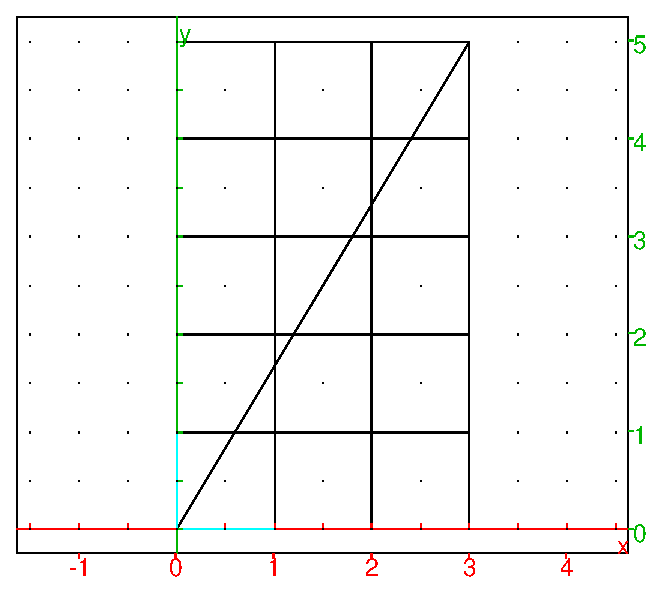
\includegraphics[width=\textwidth]{quadrillage}}
\item 
On remarque que la diagonale entre dans le premier carreau, puis elle entre 
dans un nouveau carreau lorsqu'elle coupe 
une ligne verticale ou une ligne horizontale ou \`a la fois une ligne verticale
et une ligne vhorizontale.\\
Puisqu'il y a $p-1$ verticales et $q-1$ horizontales \`a traverser, 
si la diagonale ne coupe jamais \`a la fois une verticale et une horizontale 
(c'est \`a dire si elle ne contient pas de points \`a coordonn\'ees enti\`eres
\`a part le point de d\'epart et le point d'arriv\`ee) le 
nommbre de carreaux travers\'es est $1+p-1+q-1=p+q-1$.\\ 
Si la diagonale coupe $r$ fois, une verticale et une horizontale en m\^eme 
temps, c'est \`a dire si elle contient $r+2$ points \`a coordonn\'ees 
enti\`eres (+2 en comptant le point de d\'epart et le point d'arriv\`ee) le 
nommbre de carreaux travers\'es est $p+q-1-r$.\\ 
Que vaut $r$ ?\\
La diagonale a comme \'equation $y=q*x/p =q1*x/p1$ o\`u $p=p1*d$ et $q=q1*d$ 
avec $d=$pgcd($p,q$) et elle aura des points \`a coordonn\'ees enti\`eres 
chaque fois que $x$ est entier et que $p1$ divise $q1*x$. Puisque $p1$ et $q1$ 
sont premiers entre eux, $p1$ divise $q1*x$ si $x$ est un entier multiple de $p1$. Cela se produit lorsque $0\geq x\geq p$,
pour $x=0,x=p1,x=2*p1...x=d*p1=p$, soit $d+1$ fois.\\
On a donc $r+2=d+1$ et le 
nommbre de carreaux travers\'es est $p+q-$pgcd$(p,q)$.\\ 
 \item On tape la fonction {\tt nbcarreaux} :
\begin{verbatim}
nbcarreaux(p,q):={
local d;
d:=gcd(p,q);
return p+q-d;
}
\end{verbatim}
On tape :\\
{\tt nuage\_points([x,nbcarreaux(240,x)]\$(x=0..300))}\\
On obtient :\\
\framebox{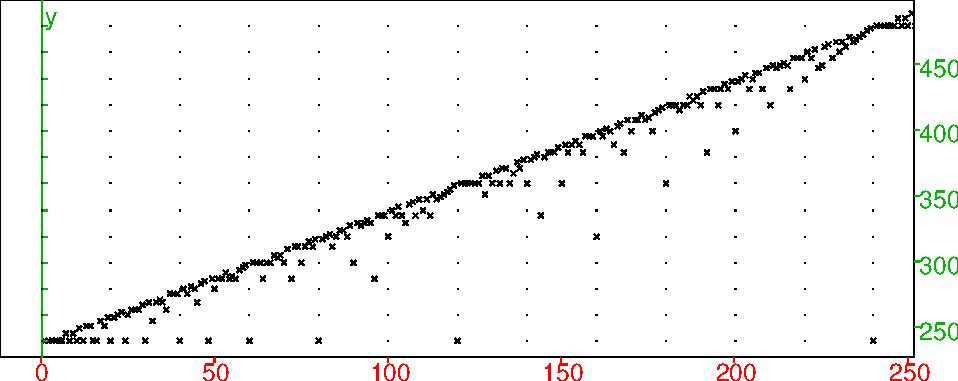
\includegraphics[width=\textwidth]{quadrillage1}}
On tape :\\
{\tt plotlist([x,nbcarreaux(240,x)]\$(x=0..300))}\\
On obtient :\\
\framebox{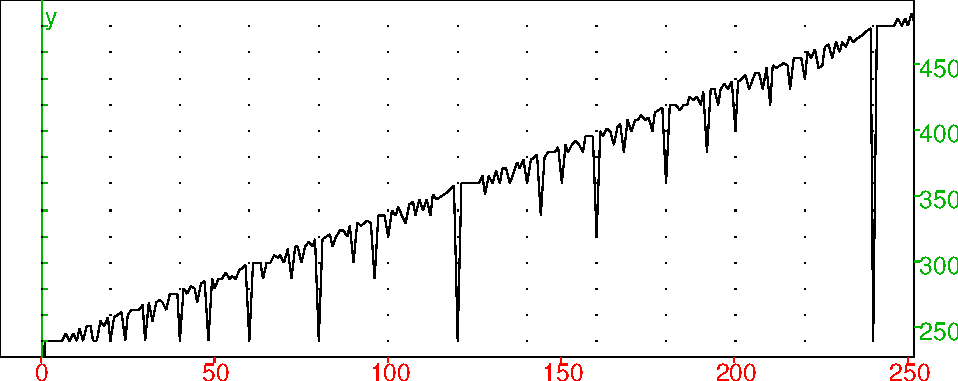
\includegraphics[width=\textwidth]{quadrillage2}}
\end{enumerate}

\section{R\'esolution dans $\N^*$ de $x^2=y^2+z^2$}
On veut r\'esoudre dans $\N^*$ : $x^2=y^2+z^2$.\\
Par exemple on veut avoir toutes les solutions de $x^2=y^2+z^2$
pour  $x \leq 200$ et $(x,y,z)\in \N^3$.\\ 
On peut \'ecrire un programme qui fait un balayage, mais cela n'est pas 
efficace car beaucoup trop long !\\
On tape :
\begin{verbatim}
triplet0(n):={
  local j,k,s,L;
  L:=NULL;
  pour j de 2 jusque n faire
    pour k de 1 jusque j-1 faire
      s:=sqrt(j^2-k^2);
      si (type(s)==DOM_INT)alors
        L:=L,[j,k,s],[j,s,k];
      fsi; 
    fpour;
  fpour;
  return L;
}
:;
\end{verbatim}
Puis :\\
{\tt A:=triplet0(200):;size(A)}\\
On obtient (Evaluation time: 2.46) :\\
{\tt Done, 254}\\
Il faut donc am\'eliorer le programme.\\
 Cette am\'elioration donne lieu \`a l'exercice suivant :

{\bf Exercice : am\'elioration}
\begin{itemize}
\item Montrer que si $(x,y,z)$ est une solution tous les multiples de $(x,y,z)$
sont aussi des solutions.\\
 En effet :\\
 $(kx)^2=k^2x^2=k^2y^2+k^2z^2=(ky)^2+(kz)^2$ pour tout $k \in \N^*$.\\
On va donc d'abord chercher les solutions pour lesquelles $(x,y,z)$ sont 
premiers entre eux. 
\item Montrer que si $(x,y,z)$ sont  premiers entre eux dans leur ensemble et 
v\'erifient $x^2=y^2+z^2$ alors  $(x,y)$ (resp $(x,z)$ ou $(y,z)$) sont 
premiers entre eux.\\
En effet :\\
soit un diviseur premier $d$ de 
$x$ et de $y$ (resp de $x$ et de $z$ ou de $y$ et de $z$) alors $d^2$ divise 
$x^2-y^2=z^2$ (resp $x^2-z^2=y^2$ ou $y^2+z^2=x^2$) donc $d$ divise $z$ (resp
$d$ divise $y$ ou $d$ divise $x$).
\item Montrer que $x$ est impair et que $y$ ou $z$ est divisible par 4.\\
En effet :\\
si $x$ est pair $x^2$ est un multiple de 4 donc $x^2=0 \bmod 4$ et\\
si $x$ est impair $x^2$ est un multiple de 4 plus 1 donc $x^2=1 \bmod 4$.\\
Supposons que $y$ et $z$ soient impairs :\\
on a  $y^2=1 \bmod 4$ et $z^2=1 \bmod 4$ donc $y^2+z^2=2 \bmod 4$
donc $y^2+z^2$ ne peut pas \^etre un carr\'e.\\
Donc $y$ ou $z$ est pair.
\item Montrer que  si $z$ est pair alors $z$ est un multiple de 4.\\
En effet si $y$ est impair et $z=2 \bmod 4$ alors $y^2+z^2=3 \bmod 4$ donc 
$y^2+z^2$ ne peut pas \^etre un carr\'e.
\item On pose  pour $a$ et $b$ quelconques dans $\N^*$ ($a>b$) :\\
$x=a^2+b^2$,\\
$y=a^2-b^2$\\
$z=2ab$\\
Montrer qu'alors on a $x^2=y^2+z^2$.\\
En effet :\\
$x^2=a^4+2a^2b^2+b^4=a^4-2a^2b^2+b^4+4a^2b^2=y^2+z^2$\\
donc $(x,y,z)$ est une solution dans $\N^*$ de $x^2-y^2=z^2$ .
\item Montrer que toutes les solutions de $x^2=y^2+z^2$ avec des nombres 
entiers premiers  entre eux dans leur ensemble sont de cette forme.\\
Soit $x,y,z$ une solution  de $x^2=y^2+z^2$ o\`u $x,y,z$ sont des 
nombres entiers premiers entre eux dans leur ensemble. On a montrer que $y$ ou 
$z$ \'etait un multiple de 4. Supposons que ce soit $z$.\\
On a :\\
$\displaystyle {(\frac{z}{2})}^2=(\frac{x+y}{2})(\frac{x-y}{2})$ et\\ 
puisque $x,y,z$ sont des nombres entiers premiers entre eux dans leur ensemble 
$x$ et $y$ sont impairs et premiers entre eux.\\
Donc $\displaystyle \frac{x+y}{2}$ et $\displaystyle \frac{x-y}{2}$ sont des 
nombres entiers qui sont premiers entre eux et comme leur produit est un 
carr\'e, ils sont eux aussi des carr\'es.\\
On pose $\displaystyle a^2=\frac{x+y}{2}$ et $\displaystyle b^2=\frac{x-y}{2}$ 
et on a :\\
$x=a^2+b^2$\\
$y=a^2-b^2$\\
$z=2*a*b$ 
\end{itemize}
On tape :
\begin{verbatim}
triplet(n):={
local a,b,a2,b2,m,q,p,k,L;
L:=NULL;
for (a:=2;a<sqrt(n);a++) {
  a2:=a^2;
  for (b:=1;b<=sqrt(n-a2) and b<a ;b++) {
    b2:=b^2;
    m:=a2+b2;p:=a2-b2;q:=2*a*b;
    if (gcd(m,p,q)==1){
      for (k:=1;k<=n/m;k++) {
        L:=L,[k*m,k*p,q*k],[k*m,k*q,p*k];
      }
    }
  } 
}
return L;
}:;
\end{verbatim}
Puis :\\
{\tt A:=triplet(200):;size(A)}\\
On obtient instantan\'ement :\\
{\tt Done, 254}\\
Dans {\tt A} on a a des triplets comme {\tt [143,55,132]} et {\tt [143,132,55]}
qui sont en fait {\tt 11*[13,5,12]}, on peut donc refaire un pogramme qui 
renverra les triplets {\tt [x,y,z]} qui v\'erifient $x^2=y^2+z^2$ avec $y>z$ et
{\tt gcd(y,z)=1}. 
On tape pour avoir les triplets $x,y,z$ v\'erifiant $x^2=y^2+z^2$ avec  
$x=a^2+b^2<n$ :
\begin{verbatim}
triplets(n):={
local a,b,a2,b2,m,q,p,k,L;
L:=NULL;
for (a:=2;a<sqrt(n);a++) {
  a2:=a^2;
  for (b:=1;b<=sqrt(n-a2) and b<a ;b++) {
    b2:=b^2;
    m:=a2+b2;p:=a2-b2;q:=2*a*b;
    if (gcd(m,p,q)==1){
      L:=L,[m,max(p,q),min(p,q)];
      }
  } 
}
return L;
}:;
\end{verbatim} 
On suppose que {\tt n} est le nombre de triplets d\'esir\'es.\label{sec:tripless}
\begin{verbatim}
tripletss(n):={
local a,b,a2,b2,m,q,p,k,L;
L:=NULL;
k:=0;
a:=2;
while (k<n) {
  a2:=a^2;
  for (b:=1;b<a and k<n;b++) {
    b2:=b^2;
    m:=a2+b2;p:=a2-b2;q:=2*a*b;
    if (gcd(m,p,q)==1){
      L:=L,[m,max(p,q),min(p,q)];
      k:=k+1;
    }
  } 
a:=a+1;
}
return L;
}:;
\end{verbatim} 
\subsection{Exercice}
Trouver les solutions en nombres entiers de $x^2=y^2+z^2$ avec $x=y+1$.
\section{Les paires carr\'ees}
\subsection{L'\'enonc\'e}
{\bf D\'efinition} \\
On dit que les entiers $p$ et $q$ est une paire carr\'ee si il existe deux 
entiers $a$ er $b$ tels que $q+p=a^2$ et $q-p=b^2$.\\
Par exemple (6,10) est une paire carr\'ee car $10-6=2^2$ et $10+6=4^2$.

{\bf Remarque} si $p$ et $q$ est une paire carr\'ee alors $2q=a^2+b^2$ et
$2p=a^2-b^2$ donc $a-b$ est pair et
$(2q)^2=(2p)^2+(2ab)^2=a^4+b^4-2a^2b^2+4a^2b^2$.\\
Donc $q^2=p^2+(ab)^2$
\begin{enumerate}
\item \'Ecrire un programme qui en balayant tous les nombres de 0 \`a $n$ 
donne les paires carr\'ees $(p,q)$ avec $0 \leq p \leq q \leq n$,
\item Montrer que si $(p,q)$ est une paire carr\'ee alors on a :
$$2q=a^2+b^2 \mbox{ et } 2p=a^2-b^2$$
\item Montrer que quelque soit $n \in \N$ on soit $n^2=1 \bmod 4$, 
soit $n^2=0 \bmod 4$. En d\'eduire alors que $p$ est pair si $(p,q)$ est une 
paire carr\'ee.\\
Modifier votre programme pour tenir compte de cette information.
\item Montrer que $a^2-b^2$ est un multiple de 4. En d\'eduire que
$a$ et $b$ ont m\^eme parit\'e et que $a-b$ est pair. \\
\'Ecrire un programme qui \`a partir de $b$ et de $a=b+2n$ calcule les valeurs
de $p$ et $q$ v\'erifiant  $q=(a^2+b^2)/2$ et $p=(a^2-b^2)/2$  et 
$0 \leq p \leq q \leq 1000$.
\item Afficher les points de coordonn\'ees $(p,q)$ 
($0 \leq p \leq q \leq 1000$) o\`u $(p,q)$ est une paire carr\'ee.
\item Trouver les \'equations des droites et des courbes en forme de filets
reliants certains de ces points.
\end{enumerate}
\subsection{La solution}
\begin{enumerate}
\item 
\begin{verbatim}
paire_carre0(n):={
local a,b,q,p,L;
L:=NULL;
pour p de 0 jusque n faire
pour q de p jusque n faire
a:=sqrt(q+p);
b:=sqrt(q-p);
si (a==floor(a) et b==floor(b)) alors
L:=L,[p,q];
fsi
fpour
fpour
return L
}:;
\end{verbatim}
ou on utilise {\tt type} pour tester si {\tt a} et {\tt b} sont des carr\'es :
\begin{verbatim}
paire_carre1(n):={
local a,b,q,p,L;
L:=NULL;
pour p de 0 jusque n faire
pour q de p jusque n faire
a:=sqrt(q+p);
b:=sqrt(q-p);
si (type(a)==DOM_INT et type(b)==DOM_INT) alors
L:=L,[p,q];
fsi
fpour
fpour
return L
}:;
\end{verbatim}
On tape :\\
{\tt L1:=paire\_carre1(100)}\\
On obtient (Evaluation time: 2.26) :
\begin{verbatim}
[0,0],[0,1],[0,4],[0,9],[0,16],[0,25],[0,36],[0,49],
[0,64],[0,81],[0,100],[2,2],[4,5],[6,10],[8,8],[8,17],
[10,26],[12,13],[12,37],[14,50],[16,20],[16,65],
[18,18],[18,82],[20,29],[24,25],[24,40],[28,53],
[30,34],[32,32],[32,68],[36,45],[36,85],[40,41],[42,58],
[48,52],[48,73],[50,50],[54,90],[56,65],[60,61],[64,80],
[70,74],[72,72],[72,97],[80,89],[84,85],[96,100],[98,98]
\end{verbatim}
On tape : {\tt dim(L1)}\\
On obtient; {\tt 49}
\item Si $(p,q)$ est une paire carr\'ee, on a :\\
$q+p=a^2$ et $q-p=b^2$\\
donc $p=(a^2-b^2)/2$, donc $a^2-b^2$ est pair c'est \`a dire 
$a^2-b^2=0 \bmod 4$, soit $a^2-b^2=2 \bmod 4$. 
\item Soit $n \in \N$ ;\\ 
si $n$ est pair alors $n^2=0 \bmod 4$, en effet, si $n=2k$ on a 
$n^2=4k^2$ et\\ 
si $n$ est impair alors $n^2=1 \bmod 4$ en effet :\\
si $n=2k+1$ on a $n^2=4k^2+4k+1$.
\item Donc on a :\\
soit $a^2-b^2=0 \bmod 4$,\\
 soit $a^2-b^2=1 \bmod 4$ \\
soit $a^2-b^2=3 \bmod 4$.\\ 
et puisque $a^2-b^2=0 $ est pair, on en d\'eduit qu $a^2-b^2=0 \bmod 4$ 
on en d\'eduit que $p$ est pair.\\
On tape :
\begin{verbatim}
paire_carre2(n):={
local a,b,q,p,L;
L:=NULL;
pour p de 0 jusque n pas 2 faire
pour q de p jusque n faire
a:=sqrt(q+p);
b:=sqrt(q-p);
si (a==floor(a) et b==floor(b)) alors
L:=L,[p,q];
fsi
fpour
fpour
return L
}:;
\end{verbatim}
On tape :\\
{\tt L2:=paire\_carre2()}\\
On obtient comme pr\'ec\'edement (Evaluation time: 1.36) :
\begin{verbatim}
[0,0],[0,1],[0,4],[0,9],[0,16],[0,25],[0,36],[0,49],
[0,64],[0,81],[0,100],[2,2],[4,5],[6,10],[8,8],[8,17],
[10,26],[12,13],[12,37],[14,50],[16,20],[16,65],
[18,18],[18,82],[20,29],[24,25],[24,40],[28,53],
[30,34],[32,32],[32,68],[36,45],[36,85],[40,41],[42,58],
[48,52],[48,73],[50,50],[54,90],[56,65],[60,61],[64,80],
[70,74],[72,72],[72,97],[80,89],[84,85],[96,100],[98,98]
\end{verbatim}
On tape : {\tt dim(L2)}\\
On obtient; {\tt 49}
\item On a si $(p,q)$ est une paire carr\'ee :
$2p=a^2-b^2$ donc $a^2-b^2$ est un multiple de 2 donc\\
$a^2$ et $b^2$ ont m\^eme parit\'e donc\\
$a$ et $b$ ont m\^eme parit\'e et donc $a-b$ est un multiple de 2 c'est \`a 
dire $a-b$ est pair.\\
On pose :\\
$a=b+2r$
donc $a^2=b^2+4rb+4r^2$ et on a :\\
$p=(a^2-b^2)/2=2rb+2r^2$ et \\
$q=(a^2+b^2)/2=b^2+2rb+2r^2=b^2+p$.\\
On veut obtenir toutes les paires carr\'ees $(p,q)$ v\'erifiant 
$0 \geq p \geq q \geq n$, donc on doit avoir :\\
$0\geq b^2 \geq n$ i.e $0\geq b \geq \sqrt n$ et\\
$0\geq 2rb+2r^2\geq n$ et $0\geq b^2+2rb+2r^2\geq n$.\\
On tape : \\
{\tt supposons(b>=0 and b<=31);}\\
{\tt simplify(solve(b\verb|^|2+2*r*b+2*r\verb|^|2<1000,r))}\\
On obtient;:\\
{\tt [((r>((-b-sqrt(-b\verb|^|2+2000))/2)) \&\& (((-b+sqrt(-b\verb|^|2+2000))/2)>r))]}\\
On tape : 
\begin{verbatim}
paire_carre(n):={
local b,q,p,L,r,nmax;
L:=NULL;
pour b de 0 jusque sqrt(n) faire
nmax:=(sqrt(-b^2+2*n))/2-b/2;
pour r de 0 jusque nmax faire
p:=2*r*b+2*r^2;
q:=b^2+p;
L:=L,[p,q];
fpour
fpour
return L
}:;
\end{verbatim}
Puis, on tape :\\
{\tt L:=paire\_carre(100):;}\\
Le calcul est tres rapide !!!!!\\
On tape : {\tt dim(L)}\\
On obtient instantan\'ement : {\tt 48}\\
On tape :\\
{\tt L3:=paire\_carre(1000):;}\\
Le calcul est tres rapide !!!!!\\
On tape : {\tt dim(L3)}\\
On obtient : {\tt 421}
\item 
On tape : {\tt nuage\_points(L3)}\\
On obtient :\\
\framebox{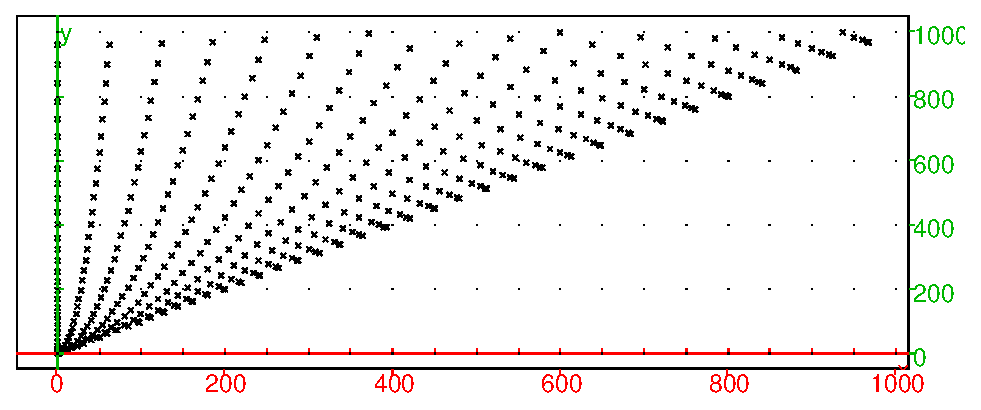
\includegraphics[width=\textwidth]{nuageL3}}
\item
On a $q=p+b^2$ donc les points sont sur les droites d'\'equations $y=x+b^2$ pour
$b$ fix\'e.\\
0n a $p=2nb+2n^2$ donc $b=(p/(2n)-n)$ donc  $q=p^2/(4n^2)+n^2$
donc les points sont sur les courbes 
d'\'equations $y=x^2/(4n^2)+n^2$ pour $n$ fix\'e.\\
On tape et on obtient :\\
\framebox{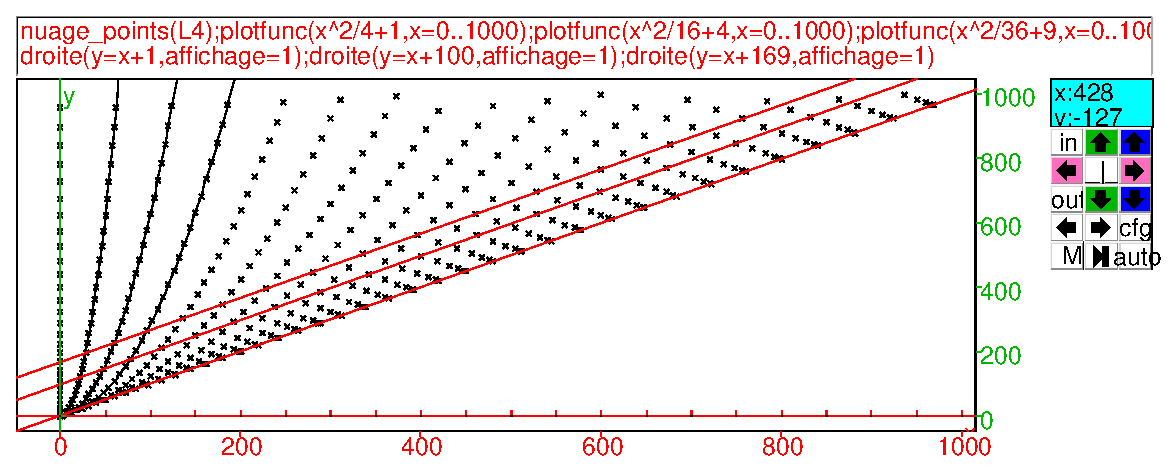
\includegraphics[width=\textwidth]{nuee}}
\end{enumerate}

\section{Les triangles rectangles presque isoc\`eles}
{\bf D\'efinition}\\
Un triangle rectangle  dont les 
c\^ot\'es sont :
\begin{enumerate}
\item les entiers $a$,$c-1$,$c$ lorsque $c$ est la longueur de 
l'hypot\'enuse est un triangle rectangle presque isoc\`ele de type 1.\\
\item les entiers $a$,$a+1$,$c$ lorsque $c$ est la longueur de 
l'hypot\'enuse est un triangle rectangle presque isoc\`ele de type 2.\\
\end{enumerate}
Pour trouver les triangles rectangles presque isoc\`eles il faut et il suffit 
de r\'esoudre en nombre entiers les \'equations 
\begin{enumerate}
\item $a^2+(c-1)^2=c^2$, c'est \`a dire :\\
trouver les couples $(a,c)\in \N$ v\'erifiant $a^2+c^2-2c+1=c^2$.\\
\item $a^2+(a+1)^2=c^2$, 
c'est \`a dire :\\
trouver les couples $(a,c)\in \N$ v\'erifiant $2a^2+2a+1=c^2$.\\
\end{enumerate}
\subsection{L'\'enonc\'e 1}
On veut trouver les triangles rectangles presque isoc\`ele de type 1.
On cherche donc les couples $(a,c)\in \N$ v\'erifiant $a^2+c^2-2c+1=c^2$ c'est 
\`a dire :\\
$a^2=2c-1$.\\
\subsection{La solution de l'\'enonc\'e 1}
$a$ est donc impair i.e. $a=2k+1$ avec $k\in \N$.\\
On a donc $4k^2+4k=2(c-1)$ et donc $c=2k^2+2k+1=k^2+(k+1)^2$\\
Les c\^ot\'es du triangle rectangle presque isoc\`ele de type 1 sont donc :\\
$[2k+1,k^2+(k+1)^2-1,k^2+(k+1)^2]$ ou encore $[2k+1,2k(k+1),k^2+(k+1)^2]$ 
lorsque $k \in \N$.\\
On tape :\\
{\tt [2k+1,2k*(k+1),k\verb|^|2+(k+1)\verb|^|2]\$(k=0..10)}
On obtient :\\
{\tt [1,0,1],[3,4,5],[5,12,13],[7,24,25],[9,40,41],[11,60,61],}\\
{\tt [13,84,85],[15,112,113],[17,144,145],[19,180,181],[21,220,221]}\\
On peut trouver une relation de r\'ecurrence entre 2 tripletssuccessifs.
On cherche $x,y,z$ tels que pour tout $k\in \N$ on ait :\\
$a_k=xa_{k-1}+yb_{k-1}+zc_{k-1}$.\\
$2k+1=x*(2k-1)+y*2k*(k-1)+z*(k^2+(k-1)^2=2k^2(z+y)+2k(x-y-z)+z-x$
Donc $y=-z$ $x-y-z=x=1$ et $z-x=1$ \\
On trouve donc $x=1,y=-2,z=2$\\
On cherche $x,y,z$ tels que :\\
$b_k=xa_{k-1}+yb_{k-1}+zc_{k-1}$.\\
On trouve $x=2,y=-1, z=2$\\
On cherche $x,y,z$ tels que :\\
$c_k=xa_{k-1}+yb_{k-1}+zc_{k-1}$.\\
On trouve $x=2,y=-2, z=3$\\
On a donc :\\
{\tt A:=[[1,-2,2],[2,-1,2],[2,-2,3]]}\\
Le $k-$i\`eme triplet est \'egal \`a $A^k*[1,0,1]$\\
On tape :\\
{\tt (A\verb|^|k*[1,0,1])\$(k=1..6) }\\
On obtient :\\
{\tt  [3,4,5],[5,12,13],[7,24,25],[9,40,41],[11,60,61],[13,84,85],}\\
{\tt [15,112,113],[17,144,145],[19,180,181],[21,220,221]}\\
{\tt P,B:=jordan(A)}\\
On obtient :\\
{\tt [[0,2,0],[4,2,0],[4,2,1]],[[1,1,0],[0,1,1],[0,0,1]]}
On a $A^k=PB^kP^{-1}$
On sait que $B^n=[[1,n,sum(k,k=1..n-1)],[0,1,n],[0,0,1]]$ donc on tape :\\
{\tt Bn:=unapply([[1,n,sum(k,k=1..n-1)],[0,1,n],[0,0,1]],n)}\\
{\tt P*Bn(5)*inv(P)*[1,0,1]}
On obtient :\\
{\tt [11,60,61]}\\
On tape :\\
{\tt subst([2k+1,2k*(k+1),k\verb|^|2+(k+1)\verb|^|2],k,5)}\\
On obtient :\\
{\tt [11,60,61]}


\subsection{L'\'enonc\'e 2}
On veut trouver les triangles rectangles presque isoc\`ele de type 2.
On cherche donc les couples $(a,c)\in \N$ v\'erifiant $2a^2+2a+1=c^2$.\\
 \begin{enumerate}
\item \'Ecrire un programme qui donne, en balayant tous les entiers $a$ de 0 
\`a $n$, les triplets $(a,a+1,c)\in \N^3$ v\'erifiant $a^2+(a+1)^2=c^2$.
Donner les solutions pour $n=1000$
\item \'Ecrire un programme qui donne les $n$ premiers tripl\'es en modifiant le programme {\tt tripless} (cf \ref{sec:tripless})
\item Montrer que si le triplet $(a,a+1,c)\in \N^3$ v\'erifie $a^2+(a+1)^2=c^2$
alors $c$ est impair et v\'erifie $2c^2-1=(2a+1)^2$.
\'Ecrire un programme qui donne les triplets $(a,a+1,c)\in \N^3$ v\'erifiant $a^2+(a+1)^2=c^2$ et qui utilise cette prori\'et\'e de $c$.
\item On consid\`ere la suite r\'ecurrente :\\
$a_0=0,\ a_1=3,\ a_{n+2}=6a_{n+1}-a_n+2\ \  (n\geq 0)$\\
Montrer par r\'ecurrence que pour tout $n\in \N$ on a :\\
$a_{n+1}^2-6a_na_{n+1}+a_n^2-2a_{n+1}-2a_n=3$
\item On consid\`ere la suite r\'ecurrente :\\
$c_0=1,\ c_1=5,\ c_{n+2}=6c_{n+1}-c_n\ \  (n\geq 0)$\\
Montrer par r\'ecurrence que pour tout $n\in \N$ on a :\\
$c_n^2=2a_n^2+2a_n+1$
 En d\'eduire que pour tout $n\in \N$, les triplets $(a_n,a_n+1,c_n)$ 
donnent des solutions.\\
On montrera dans la question 9 que l'on obtient ainsi toutes les solutions.
\item \'Ecrire un programme qui donne des triplets $(a,a+1,c)\in \N^3$ 
v\'erifiant $a^2+(a+1)^2=c^2$ et qui utilise pour $c$ la relation de 
r\'ecurrence :\\
$c_0=1,\ c_1=5,\ c_{n+2}=6c_{n+1}-c_n\ \  (n\geq 0)$.
\item On veut trouver $c_n$  en fonction de $n$.\\
D\'eterminer les progressions g\'eom\'etriques $v_n=v_0*r^n$ qui v\'erifie la 
relation de $v_{n+2}=6v_{n+1}-v_n$.\\
Puis en d\'eduire la valeur de $c_n$ en fonction de $n$.
\item On veut trouver $a_n$  en fonction de $n$.\\
D\'eterminer $p$ pour que la suite $u_n=a_n+p$ v\'erifient la 
relation de r\'ecurrence $u_{n+2}=6u_{n+1}-u_n$.\\
Puis en d\'eduire la valeur de $a_n$ en fonction de $n$
\item Montrer que l'on a :
$c_0=1,a_0=0$ et\\
$c_{n+1}=4a_n+3c_n+2$\\
$a_{n+1}=3a_n+2c_n+1$\\
et r\'eciproquement si $c_n$ et $a_n$ v\'erifient :\\
$c_0=1,\ a_0=0,$ et\\
$c_{n+1}=4a_n+3c_n+2$\\
$a_{n+1}=3a_n+2c_n+1$\\
alors \\
$c_0=1,\ c_1=5,\ c_{n+2}=6c_{n+1}-c_n\ \  (n\geq 0)$ et\\
$a_0=0,\ a_1=3,\ a_{n+2}=6a_{n+1}-a_n+2\ \  (n\geq 0)$\\
\item Montrer que l'on obtient toutes les solutions cherch\`ees
\item \'Ecrire la relation $c_{n+2}=6c_{n+1}-c_n$ sous la forme :
$$
\left(
\begin{array}{c}
c_{n+2}\\
c_{n+1}
\end{array}
\right)
=M
\left(
\begin{array}{c}
c_{n+1}\\
c_n
\end{array}
\right)$$
et d\'eterminer la matrice $M$
\item Calculer par r\'ecurrence $M^n$, pour $n\in \N$.
\item On consid\`ere les suites $w$ d\'efinies par
$w_0\in \N,\ w_{n+1}=$floor$((3+2\sqrt 2)w_n)$ (floor d\'esigne la 
partie enti\`ere)\\
Montrer qu'alors pour tout $n\in \N^*$ on a :\\
$w_{n+1}=6w_n-w_{n-1}$\\
En d\'eduire que si on choisit $w_0=1$ la suite $w_n$ est la suite  
$c_n$ qui donne la longueur des hypot\'enuse des triangles rectangles presque 
isoc\`eles.\\
En d\'eduire que si $w_0=1$ alors $2*w_n^2-1$ est le carr\'e de 
$2a_n+1$.\\
\'Ecrire un programme qui donne les triplets $(a,a+1,c)\in \N^3$ v\'erifiant 
$a^2+(a+1)^2=c^2$ et qui utilise cette d\'efinition de $c$.
\item \'Ecrire les relations de r\'ecurrence :\\
$c_n=4a_{n-1}+3c_{n-1}+2$ et $a_n=3a_{n-1}+2c_{n-1}+1$\\ 
avec une matrice 3x3.
\item On consid\`ere les suites $v$ d\'efinies par
$v_0\in \N,\ v_{n+1}=$3+floor$((3+2\sqrt 2)v_n)$ (floor d\'esigne la 
partie enti\`ere)\\
Montrer qu'alors pour tout $n\in \N^*$ on a :\\
$v_{n+1}=6v_n-v_{n-1}+2$\\
En d\'eduire que si on choisit $v_0=0$ la suite $v_n$ est la suite  
$a_n$ qui donne la longueur du plus petit cot\'e des triangles rectangles 
presque isoc\`eles.\\
En d\'eduire que si $v_0=0$ et $w_0=1$ alors $2*w_n^2-1=(2v_n+1)^2$.\\
\'Ecrire un programme qui donne les triplets $(a,a+1,c)\in \N^3$ v\'erifiant 
$a^2+(a+1)^2=c^2$ et qui utilise cette d\'efinition de $a$ et $c$.
\end{enumerate}
\subsection{La solution de l'\'enonc\'e 2}
\begin{enumerate}
\item 
On tape :
\begin{verbatim}
rectpiso1(n):={
local a,c,d,L;
L:=NULL;
pour a de 0 jusque n faire 
d:=2a^2+2a+1;
c:=round(sqrt(d));
si c^2==d alors L:=L,[a,a+1,c];fsi;
fpour;
retourne L;
}:;
\end{verbatim}
On tape :\\
{\tt rectpiso1(10000)}\\
On obtient (Evaluation time: 12.73):\\
{\tt [0,1,1],[3,4,5],[20,21,29],[119,120,169],[696,697,985], [4059,4060,5741]}
\item On change le test {\tt if (gcd(m,p,q)==1)} en :\\
{\tt if (gcd(m,p,q)==1 and abs(p-q)==1)} et on tape
\begin{verbatim}
triplets2(n):={
local a,b,a2,b2,m,q,p,k,L;
L:=NULL;
k:=0;
a:=2;
while (k<n) {
  a2:=a^2;
  for (b:=1;b<a and k<n;b++) {
    b2:=b^2;
    m:=a2+b2;p:=a2-b2;q:=2*a*b;
    if (gcd(m,p,q)==1 and abs(p-q)==1){
      L:=L,[m,max(p,q),min(p,q)];
      k:=k+1;
    }
  } 
a:=a+1;
}
return L;
}:;
\end{verbatim} 
On tape :\\
{\tt triplets2(5)}\\
On obtient :\\
{\tt [5,4,3],[29,21,20],[169,120,119],[985,697,696],[5741,4060,4059]}
\item 
Puisque $c^2=a^2+(a+1)^2=2a^2+2a+1$ on en d\'eduit que $c^2$ est un entier 
impair donc $c$  est un entier impair.\\
On a aussi :
  $2c^2-1=4a^2+4a+1=(2a+1)^2$\\
On tape :
\begin{verbatim}
rectpiso2(n):={
local a,c,d,L;
L:=NULL;
pour c de 1 jusque n pas 2 faire 
d:=2c^2-1;
a:=round(sqrt(d));
si a^2==d alors a:=(a-1)/2; L:=L,[a,a+1,c];fsi;
fpour;
retourne L;
}:;
\end{verbatim}
On tape :\\
{\tt rectpiso2(10000)}\\
On obtient (Evaluation time: 5.9) :\\
{\tt [0,1,1],[3,4,5],[20,21,29],[119,120,169],[696,697,985], [4059,4060,5741]}
\item
Pour $n=0$ on a :\\
$a_{n+1}^2-6a_na_{n+1}+a_n^2-2a_{n+1}-2a_n=3^2-2*3=3$\\
Supposons que pour $n\in \N$ on a :\\
$a_{n+1}^2-6a_na_{n+1}+a_n^2-2a_{n+1}-2a_n=3$\\
Calculons :\\
$a_{n+2}^2-6a_{n+1}a_{n+2}+a_{n+1}^2-2a_{n+2}-2a_{n+1}$\\
sachant que :\\
$a_{n+2}=6a_{n+1}-a_n+2$\\
Dans {\tt Xcas}, {\tt a2} d\'esigne $a_{n+2}$,{\tt a1} d\'esigne $a_{n+1}$ et 
{\tt a0} d\'esigne $a_n$.\\
On tape :\\
{\tt a2:=6a1-a0+2}\\
{\tt normal(a2\verb|^|2-6a1*a2+a1\verb|^|2-2a2-2a1)}\\
On obtient :\\
{\tt a0\verb|^|2-6*a0*a1-2*a0+a1\verb|^|2-2*a1}\\
Donc :\\
$a_{n+2}^2-6a_{n+1}a_{n+2}+a_{n+1}^2-2a_{n+2}-2a_{n+1}=a_{n+1}^2-6a_na_{n+1}+a_n^2-2a_{n+1}-2a_n=$ \\
Donc, d'apr\`es l'hypoth\`ese de r\'ecurrence on a :\\
$a_{n+2}^2-6a_{n+1}a_{n+2}+a_{n+1}^2-2a_{n+2}-2a_{n+1}=3$\\
Donc, pour tout $n\in\N$, on a :
$$a_{n+1}^2-6a_na_{n+1}+a_n^2-2a_{n+1}-2a_n=3$$
\item
Pour $n=0$ on a :\\
$c_0^2=2a_0^2+2a_0+1=1$ (puisque $a_0=0$)\\
Pour $n=1$ on a :\\
$c_1^2=2a_1^2+2a_1+1=18+6+7=25$ (puisque $a_1=3$)\\
Supposons que pour $n\in \N$ on ait :\\
$c_n^2=2a_n^+2a_n+1$\\
$c_{n+1}^2=2a_{n+1}^2+2a_{n+1}+1$\\
Dans {\tt Xcas}, {\tt c2} d\'esigne $c_{n+2}$,{\tt c1} d\'esigne $c_{n+1}$ et 
{\tt c0} d\'esigne $c_n$.\\
On tape :\\
{\tt c2:=6c1-c0}\\
{\tt normal(c2\verb|^|2)}\\
On obtient :\\
{\tt c0\verb|^|2-12*c0*c1+36*c1\verb|^|2}\\
On a d'apr\`es l'hypoth\`ese de r\'ecurrence :
{\tt c0\verb|^|2=2a0\verb|^|2+2a0+1} et\\
 {\tt c1\verb|^|2=2a1\verb|^|2+2a0+1} :\\
Donc si on pose {\tt C=c2\verb|^|2}, on a :\\
{\tt C:=normal(2a0\verb|^|2+2a0+1+36*(2a1\verb|^|2+2a1+1)-12c0*c1)}\\
On obtient :\\
{\tt 2*a0\verb|^|2+2*a0+72*a1\verb|^|2+72*a1-12*c0*c1+37}\\
On tape :\\
{\tt A:=normal(2a2\verb|^|2+2a2+1)}\\
On obtient :\\
{\tt -a0\verb|^|2+6*a0*a1+2*a0-a1\verb|^|2+2*a1+3}\\
On veut montrer que {\tt C=A}.\\
On tape :\\
{\tt normal((C-A)/12)}\\
On obtient :\\
{\tt 2*a0*a1+a0+a1-c0*c1+2}\\
Il faut donc montrer que :\\
$c0*c1=2*a0*a1+a0+a1$ ou encore que :\\
$c0^2*c1^2=(2*a0*a1+a0+a1+2)^2$ ou encore que :\\
$(2a0^2+2a0+1)*(2a1^2+2a1+1)-(2*a0*a1+a0+a1+2)^2=0$\\
On tape :\\
{\tt normal((2a0\verb|^|2+2a0+1)*(2a1\verb|^|2+2a1+1)-(2*a0*a1+a0+a1+2)\verb|^|2)}\\
On obtient :\\
{\tt a0\verb|^|2-6*a0*a1-2*a0+a1\verb|^|2-2*a1-3}\\
qui vaut bien 0 d'apres la question 2.\\
Donc pour tout $n\in \N$ on a $c_n^2=2a_n^2+2a_n+1=a_n^2+(a_n+1)^2$.\\
Donc le triplet ($a_n,a_n+1,c_n$) est une solution pour tout $n$.\\
On peut montrer que l'on obtient ainsi toutes les solutions (cf question9).
\item On tape :
\begin{verbatim}
rectpiso3(n):={
local a,c,d,L,c0,c1;
c0:=1;
c1:=5;
L:=[0,1,1];
tantque c1<n faire
d:=2*c1^2-1;
a:=(sqrt(d)-1)/2;
L:=L,[a,a+1,c1];
c:=c1;
c1:=6*c1-c0;
c0:=c;
ftantque;
retourne L;
}:;
\end{verbatim}
On tape :\\
{\tt rectpiso3(10000)}\\
On obtient (instantan\'ement):\\
{\tt [0,1,1],[3,4,5],[20,21,29],[119,120,169],[696,697,985], [4059,4060,5741]}
\item
Si $v_n=v_0*r^n$ v\'erifie $v_{n+2}=6v_{n+1}-v_n$ c'est que $r$ est solution de 
$x^2-6x+1=0$.\\
On tape :\\
{\tt r1,r2:=solve(x\verb|^|2-6x+1,x)}\\
On obtient :\\
{\tt [-2*sqrt(2)+3,2*sqrt(2)+3]}\\
Donc il y a 2 progressions g\'epm\'etriques de raison $r1=-2\sqrt 2+3$ et
$r2=2\sqrt 2+3$ qui verifient aussi cette relation de r\'ecurence.\\
Une combinaison lineaire de suites verifiant 
$v_{n+2}=6v_{n+1}-v_n$  verifient aussi cette relation de r\'ecurence.\\
Donc la suite :\\
$w_n=x*r1^n+y*r2^n$ v\'erifie $w_{n+2}=6w_{n+1}-w_n $ quelque soit $x$ et $y$.\\
Puisque la suite $c_n$ est enti\`erement d\'etermin\'ee par $c_0=1$, $c_1=5$ et 
par la relation de r\'ecurence $c_{n+2}=6c_{n+1}-c_n$, pour avoir $c_n=w_n$ il 
suffira d'avoir $c_0=w_0$ et $c_1=w_1$ c'est \`a dire :\\
$x+y=1$ et $x*r1+y*r2=5$.\\
On tape :\\
{\tt linsolve([x+y=1,x*r1+y*r2=5],[x,y])}\\
On obtient :\\
{\tt [(-(sqrt(2))+2)/4,(sqrt(2)+2)/4]}\\
Donc :
$$c_n=\frac{2-\sqrt 2}{4}*(-2*\sqrt 2+3)^n+\frac{2+\sqrt 2}{4}*(2*\sqrt 2+3)^n$$
\item
On cherche $p$ pour que la suite $u_n=p+a_n$ v\'erifient la 
relation de $u_{n+2}=6u_{n+1}-u_n$.
On sait que $a_n$ v\'erifie $a_{n+2}=6a_{n+1}-a_n+2$ donc $p$ doit v\'erifier :\\
$p+a_{n+2}=6p+6a_{n+1}-p-a_n$ donc $p+2=6p-p$.\\
On tape :\\
{\tt solve(p+2=6p-p,p)}\\
On obtient :\\
{\tt [1/2]}\\
Donc comme pr\'ec\'edemment on va d\'eterminer la suite $a_n+1/2$.\\
Pour cela  on cherche $x$ et $y$ tel que :\\
$x+y=a_0+1/2=1/2$ et $x*r1+y*r2=a_1=3+1/2=7/2$\\
On tape :\\
{\tt normal(linsolve([x+y=1/2,x*r1+y*r2=7/2],[x,y]))}\\
On obtient :\\
{\tt [(-(sqrt(2))+1)/4,(sqrt(2)+1)/4]}\\
On a donc :\\
$u_n=\frac{1-\sqrt 2}{4}*(-2*\sqrt 2+3)^n+\frac{1+\sqrt 2}{4}*(2*\sqrt 2+3)^n$\\
Donc :
$$a_n=-\frac{1}{2}+\frac{1-\sqrt 2}{4}*(-2*\sqrt 2+3)^n+\frac{1+\sqrt 2}{4}*(2*\sqrt 2+3)^n$$
On tape :\\
{\tt c(n):=((-sqrt(2)+2)/4)*(-2*sqrt(2)+3)\verb|^|n+\\ ((sqrt(2)+2)/4)*(2*sqrt(2)+3)\verb|^|n}\\
{\tt a(n):=((-sqrt(2)+1)/4)*(-2*sqrt(2)+3)\verb|^|n+\\ ((sqrt(2)+1)/4)*(2*sqrt(2)+3)\verb|^|n-1/2}\\
{\tt normal(a(5),a(5)+1,c(5))}\\
On obtient :\\
{\tt 4059,4060,5741}\\
On tape :\\
{\tt normal(a(6),a(6)+1,c(6))}\\
On obtient :\\
{\tt 23660,23661,33461}\\
On tape :\\
{\tt normal(a(10),a(10)+1,c(10))}\\
On obtient :\\
{\tt 27304196,27304197,38613965}
\item On suppose que pour tout $n \in \N$ on a :\\
$c_0=1,\ c_1=5,\ a_0=0,\ a_1=3$ et\\
$c_{n+2}=6c_{n+1}-c_n$ et\\
$a_{n+2}=6a_{n+1}-a_n+2$\\
Montrons par r\'ecurrence qu'alors pour tout $n \in \N$ on a :\\
$c_0=1,\ a_0=0$ et\\
$c_{n+1}=4a_n+3c_n+2$\\
$a_{n+1}=3a_n+2c_n+1$
La relation est vrai pour $n=0$ et $n=1$ car :\\
$c_1=4*0+3*+2=5$ et\\ 
$a_1=3*0+2*1+1=3$\\
Si la relation est vrai pour $n$ on a :
$c_n=4a_{n-1}+3c_{n-1}+2$\\
$a_n=3a_{n-1}+2c_{n-1}+1$\\
alors \\
$3c_n-c_{n-1}=12a_{n-1}+8c_{n-1}+6=4a_n+2$\\
et\\
$3a_n-a_{n-1}=8a_{n-1}+6c_{n-1}+3=2c_n-1$\\
donc \\
$c_{n+1}=3c_n+3c_n-c_{n-1}=3c_n+4a_n+2$\\
et\\
$a_{n+1}=3a_n+3a_n-a_{n-1}+2=3a_n+2c_n+1$\\
R\'eciproquement si pour tout $n \in \N$ on a :\\
$c_0=1,\ a_0=0$ et\\
$c_{n+1}=4a_n+3c_n+2$\\
$a_{n+1}=3a_n+2c_n+1$\\
Alors :\\
$c_0=1,\ a_0=0$ et $c_1=4*0+3*1+2=5,\ a_1=3*0+2*1+1=3$ et\\
$3c_{n+1}-4a_{n+1}=c_n+2$ \\
$2c_{n+1}-3a_{n+1}=-a_n+1$\\
soit\\
$4a_{n+1}=3c_{n+1}-c_n-2$\\
$2c_{n+1}=3a_{n+1}-a_n+1$\\
et puisque :
$c_{n+2}=4a_{n+1}+3c_{n+1}+2$\\
$a_{n+2}=3a_{n+1}+2c_{n+1}+1$\\
on en d\'eduit que pour tout $n \in \N$:\\
$c_{n+2}=6c_{n+1}-c_n$\\
$a_{n+2}=6a_{n+1}-a_n+2$

\item
Supposons que l'on ait $(a+1)^2+a^2=2a^2+2a+1=c^2$.\\
Alors $c$ est impair et $a$ et $c$ sont premiers entre eux.\\
On a aussi : $2c^2=(2a+1)^2+1$\\
{\bf Si $a$ est pair}\\
0n a :\\
$(a+1)^2=c^2-a^2=(c+a)(c-a)$\\
donc si $d$ divise $a+1$, $d$ divise soit $c+a$, soit $c-a$ mais $d$ ne divise 
pas $c+a$ et $c-a$ car $a$ et $c$ sont premiers entre eux donc :\\
il existe $p$ et $q$ tel que  $c+a=p^2$ et $c-a=p^2$ et $pq=a+1$
On a donc $p\geq q$ avec $p$ et $q$ sont impairs et,\\
$2a=p^2-q^2$ et $2c=p^2+q^2$.\\
La relation $4c^2=8a^2+8a+4$ donne comme relation entre $p$ et $q$ :\\
$(p^2+q^2)^2=2(p^2-q^2)^2+4(p^2-q^2)+4$\\
donc\\
$p^4+q^4-6p^2q^2+4p^2-4q^2+4=0$\\
Posons\\
$X=p^2$\\
$Y=q^2$
$X$ et $Y$ sont des carr\'es d'entiers qui v\'erifient :\\
$Y^2-2Y(2+3X)+(X+2)^2$\\
Le discriminant de ce trin\^ome en $Y$ est donc le carr\'e d'un entier, c'est 
\`a dire $2X+2$ est le carr\'e d'un entier puisque :\\
$(2+3X)^2-(X+2)^2=8X^2+8X=(2p)^2(2X+2)$.\\
En posant $p=2*p_1+1$ on en d\'eduit que $X=4p_1^2+4p_1+1$ et que 
$2X+2=8p_1^2+8p_1+4=4(2p_1^2+2p_1+1)$ et donc qu'il existe 
$k \in \N$ tel que :\\
$2p_1^2+2p_1+1=k^2$\\
et on a alors :\\
$Y=q^2=(2+3p^2)-4kp$ (avec le signe "-" car $q< p$)\\
donc si $2a^2+2a+1=c^2$ avec $a$ est pair,  il existe $p$ avec $p=2*p_1+1$ et 
$k$ v\'erifiant $2p_1^2+2p_1+1=k^2$ (ou $2k^2=p^2+1$) tel que :\\
$2a=p^2-q^2=X-Y=4kp-2-2p^2=4kp-4k^2=4k(p-k)$\\
$2c=p^2+q^2=X+Y=4p^2+2-4kp=8k^2-4kp-2=2(4k^2-2kp-1)$\\
R\'eciproquent si on a $2p_1^2+2p_1+1=k^2$ pour $p_1 \in \N^*$ et $k \in \N$
alors si on pose $p=2*p_1+1$ on a  $2k^2=(2p_1+1)^2+1=p^2+1$ et :\\
$a=2kp-1-p^2=2k(p-k)$\\
$c=4k^2-2kp-1$\\
$a$ est pair $a>p_1>0$, $c>k$ et on v\'erifie que  $2a^2+2a+1=c^2$, pour cela, 
on tape :\\
{\tt a:=2k*p-k\verb|^|2}\\
{\tt c:=4k\verb|^|2-1-2k*p}\\
{\tt factor(2a\verb|^|2+2a+1-c\verb|^|2)}\\
On obtient :\\
{\tt 2*p\verb|^|2*(2*k\verb|^|2-p\verb|^|2-1)}\\
Donc puisque $2k^2=p^2+1$ on a $2a^2+2a+1=c^2$\\
{\bf Si $a$ est impair alors $a+1$ est pair}\\
0n fait le m\^eme genre de raisonnement :\\
$a^2=c^2-(a+1)^2=(c+a+1)(c-a-1)$\\
donc si $d$ divise $a$, $d$ divise soit $c+a+1$, soit $c-a-1$ mais $d$ ne 
divise pas $c+a+1$ et $c-a-1$ car $a$ et $c$ sont premiers entre eux donc :\\
il existe $p$ et $q$ tel que  $c+a+1=p^2$ et $c-a-1=p^2$ et $pq=a$.\\
On a $p\geq q$ et $p$ et $q$ sont impairs et,\\
$2a=p^2-q^2-2$ et $2c=p^2+q^2$.\\
Posons\\
$X=p^2$\\
$Y=q^2$
$X$ et $Y$ sont des carr\'es d'entiers qui v\'erifient :\\
$X^2-2X(2+3Y)+(Y+2)^2$\\
(m\^eme \'equation en \'echangeant $Y$ et $X$)\\
$2Y+2$ est un carr\'e en posant $q=2q_1+1$ cela veut dire qu'il existe 
$r \in \N$ tel que : $2q_1^2+2q_1+1=r^2$ ou encore $2r^2=q^2+1$\\
et alors $X=3Y+2+4qr=3q^2+2+4qr$ (avec le signe "+" car $X=p^2>q^2$)
donc:\\
$2a=p^2-q^2-2=2q^2+4qr=2(q^2+1)-2+4qr=2(2r^2+2qr-1)$\\
$2c=p^2+q^2=4q^2+4qr+2=4(q^2+1)-2+4qr=2(4r^2+2qr-1)$\\
R\'eciproquent si on a $2q_1^2+2q_1+1=r^2$ pour $q_1 \in \N$ et $r \in \N$
alors si on pose $q=2*q_1+1$ on a  $2r^2=(2q_1+1)^2+1=q^2+1$ et :\\
$a=2r^2+2qr-1$\\
$c=4r^2+2qr-1$\\
$a$ est impair et on tape :\\
{\tt a:=2r\verb|^|2+2q*r-1}\\
{\tt c:=4r\verb|^|2+2q*r-1}\\
{\tt factor(2a\verb|^|2+2a+1-c\verb|^|2)}\\
On obtient :\\
{\tt 2*q\verb|^|2*(2*r\verb|^|2-q\verb|^|2-1)}\\
Donc puisque $2r^2=q^2+1$ on a $2a^2+2a+1=c^2$.\\
{\bf Conclusion}
Si  $a_1,c_1$ est une solution de $2a^2+2a+1=c^2$ alors cette solution engendre
2 nouvelles solutions qui sont :\\
$a_2=2c_1(2a_1-c_1+1)$ et $c_2=(2a_1+1)^2+2c_1(c_1-2a_1-1)$\\
$a_3=(2a_1+1)^2+2(2a_1+1)c_1$ et $c_3=2(2a_1+1)^2+2(2a_1+1)c_1+1$\\
puis la solution $a_2,c_2$ engendre 2 nouvelles solutions qui sont :\\
$a_4=2c_2(2a_2+1-c_2)$ et $c_4=(2a_2+1)^2+2c_2(c_2-2a_2-1)$\\
$a_5=(2a_2+1)^2+2(2a_2+1)c_2$ et $c_5=2(2a_2+1)^2+2(2a_2+1)c_2+1$\\
On remarquera que la solution $[0,1]$ engendre $[0,1]$ et $[3,5]$, que la 
solution $s_1=[3,5]$ engendre $s_2=[20,29]$ et $s_3=[119,169]$ etc...par ce 
processus la solution $s_n$ engendre les solutions $s_{2n}$ et $s_{2n+1}$, puis 
la solution $s_{n+1}$ engendre les solutions $s_{2n+2}$ et $s_{2n+3}$ etc...\\
Pour faire le lien avec les suites pr\'ec\'edentes, il reste a montrer que la 
suite $[a_n,c_n]$ ainsi engendr\'ee v\'erifie :\\
$c_n=4a_{n-1}+3c_{n-1}+2$ et $a_n=3a_{n-1}+2c_{n-1}+1$\\
On utilise {\tt Xcas} pour faire les calculs.\\
Si $s_n=${\tt [a,c]} et $s_{n+1}=${\tt a1,c1)} sont des solutions successives, 
on d\'esigne $s_{2n}$ par {\tt [sa1(a,c),sc1(a,c)]}, $s_{2n+1}$ par {\tt [sa2(a,c),sc2(a,c)]} et $s_{2n+2}$ par {\tt [sa1(a1,c1),sc1(a1,c1)]}.\\
On d\'esigne par {\tt rc(a,c)} et par {\tt ra(a,c)} les relations de 
r\'ecurrence qui donne $c_{n+1}$ et $a_{n+1}$ en fonction de $a_n$ et $c_n$.\\
On suppose que les relations de r\'ecurrence sont v\'erifi\'ees par $s_n$ et 
$s_{n+1}$ i.e. que {\tt a1=ra(a,c)} et {\tt c1=rc(a,c)}.\\
On tape les d\'efinitions :\\
{\tt sa1(a,c):=normal(4*c*a+2*c-2*c\verb|^|2)}\\
{\tt sc1(a,c):=normal(4*c\verb|^|2-4*c*a-2*c-1)}\\
{\tt sa2(a,c):=normal(4*c*a+2*c-1+2*c\verb|^|2)}\\
{\tt sc2(a,c):=normal(4*c\verb|^|2+4*c*a+2*c-1)}\\
{\tt rc(a,c):=4*a+3*c+2;}\\
{\tt ra(a,c):=3*a+2*c+1}\\
On tape :\\
{\tt normal(rc(sa1(a,c),sc1(a,c))-sc2(a,c))}\\
On obtient : {\tt 0}\\ 
On tape :\\
{\tt normal(ra(sa1(a,c),sc1(a,c))-sa2(a,c))}\\
On obtient : {\tt 0}\\ 
On tape :\\
{\tt factor(ra(sa2(a,c),sc2(a,c))-sa1(ra(a,c),rc(a,c)))}\\
On obtient : {\tt -8*(2*a\verb|^|2+2*a-c\verb|^|2+1)}\\ 
On tape :\\
{\tt factor(rc(sa2(a,c),sc2(a,c))-sc1(ra(a,c),rc(a,c)))}\\
On obtient : {\tt -8*(2*a\verb|^|2+2*a-c\verb|^|2+1)}\\ 
ce qui donne bien {\tt 0} puisque $2a^2+2a+1=c^2$ car $s_n=${\tt [a,c]} est 
une solution de cette \'equation par hypoth\`ese.\\

On a ainsi montrer que si :\\
$s_n=${\tt [a,c]} et $s_{n+1}=${\tt a1,c1)} sont des solutions successives qui 
v\'erifient les relations de r\'ecurrence alors $s_{2n}$, $s_{2n+1}$, $s_{2n+2}$ v\'erifient aussi les relations de r\'ecurrence.\\
$s_1=[3,5]$ engendre $s_2=[20,29]$ et $s_3$.
On peut v\'erifier par le programme de la question 1 que $[3,5]$ et $[20,29]$
sont 2 solutions successives qui v\'erifie la relation de r\'ecurrence 
(29=4*3+3*5+2 et 20=3*3+2*5+1) donc on en d\'eduit par r\'ecurrence que :
si $s_2$ engendre $s_4$et $s_5$, alors $s_2,s_3,s_4$ sont des solutions 
successives qui v\'erifient la relation de r\'ecurrence....
On peut aussi faire le programme suivant qui renvoie la liste des solutions en 
utilisant les fonctions {\tt sa1, sc1, sa2, sc2} d\'efinies pr\'ec\'edemment :
\begin{verbatim}
sa1(a,c):=normal(4*c*a+2*c-2*c^2);
sc1(a,c):=normal(4*c^2-4*c*a-2*c-1);
sa2(a,c):=normal(4*c*a+2*c-1+2*c^2);
sc2(a,c):=normal(4*c^2+4*c*a+2*c-1);
tripisoc(n):={
local a,a1,a2,c,c1,c2,L,k;
L:=[0,1],[3,5];
pour k de 1 jusque n faire 
a,c:=L[k];
L:=L,[sa1(a,c),sc1(a,c)],[sa2(a,c),sc2(a,c)];
fpour;
return L;
}:;
\end{verbatim}
\item 0n a :\\
$c_{n+2}=6c_{n+1}-c_n$ et\\
$c_{n+1}=c_{n+1}$ \\
donc\\
$$ M=\left(
\begin{array}{cc}
6&-1\\
1&0
\end{array}
\right)
$$
\item Si
$$ M^n=\left(
\begin{array}{cc}
p_n&q_n\\
s_n&t_n
\end{array}
\right)
$$
On a :\\
$p_0=1$, $q_0=0$, $s_0=0$, $t_0=1$,
$p_1=6$, $q_1=-1$, $s_1=1$, $t_0=0$
$M^{n+1}=M*M^n$ c'est \`a dire :\\
$p_{n+1}=6p_n-s_n$, $q_{n+1}=6q_n-t_n$, $s_{n+1}=p_n$, $t_{n+1}=q_n$\\
donc
$p_{n+1}=6p_n-p_{n-1}$ avec $p_0=1$ et $p_1=6$\\
$q_{n+1}=6q_n-q_{n-1}$ avec $q_0=0$ et $q_1=-1$\\
Les suites $p_n$ et $q_n$ v\'erifient la m\^eme relation de r\'ecurrence que 
$c_n$ donc :\\
$p_n$ et $q_n$ sont des combinaisons lin\'eaires des 2 progressions g\'eom\'etriques de raison $r1=-2\sqrt 2+3$ et $r2=2\sqrt 2+3$.\\
Calcul de $p_n=x(r1)^n+y(r2)^n$\\ 
Pour trouver $p_n$ en fonction de $n$ il faut donc r\'esoudre :\\
$[x+y=1=p_0,x*r1+y*r2=6=p_1]$\\
On tape :\\
{\tt r1,r2:=solve(x\verb|^|2-6x+1,x)}\\
On obtient :\\
{\tt [-2*sqrt(2)+3,2*sqrt(2)+3]}\\
On tape :\\
{\tt linsolve([x+y=1,x*r1+y*r2=6],[x,y])}\\
On obtient :\\
{\tt [(-3*sqrt(2)+4)/8,(3*sqrt(2)+4)/8]}\\
Calcul de $q_n=x(r1)^n+y(r2)^n$\\ 
Pour trouver $q_n$ en fonction de $n$ il faut donc r\'esoudre :\\
$[x+y=0=q_0,x*r1+y*r2=1=q_1]$\\
On tape :\\
{\tt linsolve([x+y=0,x*r1+y*r2=1],[x,y])}\\
On obtient :\\
{\tt [(-(sqrt(2)))/8,(sqrt(2))/8]}\\
Donc pour $n\in \N$ :\\
$p_n=(-3\sqrt 2+4)(-2\sqrt 2+3)^n+(3\sqrt 2+4)(2\sqrt 2+3)^n$\\
$q_n=-\sqrt 2(-2\sqrt 2+3)^n+\sqrt 2(2\sqrt 2+3)^n$

\item On peut aussi \'ecrire la relation de r\'ecurrence :\\
$c_n=4a_{n-1}+3c_{n-1}+2$\\ 
$a_n=3a_{n-1}+2c_{n-1}+1$\\
en utilisant $A$ une matrice 3x3 :
$$ 
A=\left(
\begin{array}{ccc}
3&4&2\\
2&3&1\\
0&0&1
\end{array}
\right)
$$
et ainsi, on a :\\
$$
\left(
\begin{array}{c}
c_{n+1}\\
a_{n+1}\\
1
\end{array}
\right)
=A
\left(
\begin{array}{c}
c_n\\
a_n\\
1
\end{array}
\right)
$$
On a donc :\\
$$
\left(
\begin{array}{c}
c_n\\
a_n\\
1
\end{array}
\right)
=A^n
\left(
\begin{array}{c}
1\\
0\\
1
\end{array}
\right)
$$
On v\'erifie en tapant :\\
{\tt normal(rsolve([a(n+1)=3*a(n)+2*c(n)+d(n),\\
c(n+1)=4*a(n)+3*c(n)+2*d(n),\\
d(n+1)=d(n)],[a(n),c(n),d(n)],[a(0)=0,c(0)=1,d(0)=1]))}
On obtient :\\
{\tt [[(-(sqrt(2))+1)/4*(-2*sqrt(2)+3)\verb|^|n+\\
(sqrt(2)+1)/4*(2*sqrt(2)+3)\verb|^|n+(-1)/2,\\
(-(sqrt(2))+2)/4*(-2*sqrt(2)+3)\verb|^|n+\\(sqrt(2)+2)/4*(2*sqrt(2)+3)\verb|^|n,\\
1]]}
\item On consid\`ere la suite :\\
$w_0\in \N^*,\ w_{n+1}=$floor$(3+2*\sqrt 2)*w_n)$ (floor d\'esigne la partie 
enti\`ere)\\
On veut montrer que pour tout $n\in \N^*$ on a $w_{n+1}+w_{n-1}=6w_n$.\\
On a :\\
$w_{n+1}\leq (3+2*\sqrt 2)*w_n<w_{n+1}+1$\\
Donc :\\
$(3+2*\sqrt 2)*w_n-1<w_{n+1}\leq (3+2*\sqrt 2)*w_n$\\
On a :\\
$w_n\leq (3+2*\sqrt 2)*w_{n-1}<w_n+1$\\
Puisque $\displaystyle \frac{1}{3+2*\sqrt 2}=3-2*\sqrt 2$ on a :\\
$w_n*(3-2*\sqrt 2)\leq w_{n-1})<(w_n+1)*(3-2*\sqrt 2)$\\
Donc :\\
$(3+2*\sqrt 2)*w_n-1+w_n*(3-2*\sqrt 2)<w_{n+1}+w_{n-1}<(3+2*\sqrt 2)*w_n+(w_n+1)*(3-2*\sqrt 2)$\\
Donc :\\
$6w_n-1<w_{n+1}+w_{n-1}<6w_n+(3-2*\sqrt 2)<6w_n+1$.\\
Comme $w_{n+1}+w_{n-1}$ est un entier, on en d\'eduit qwe :\\
 $w_{n+1}+w_{n-1}=6w_n$.\\
Pour montrer que $w_n$ est la suite $c_n$ il suffit de montrer que $w_1=5$
lorsque $w_0=1$.\\
On a bien $w_1=floor(3+2*\sqrt 2)=5$, donc $w_n$ et $c_n$ coincident.\\
On tape :
\begin{verbatim}
rectpiso5(n):={
local a,c,d,L;
L:=NULL;
c:=1;
tantque c<n faire
d:=2*c^2-1;
a:=(sqrt(d)-1)/2;
L:=L,[a,a+1,c];
c:=floor((3+2*sqrt(2))*c);
ftantque;
retourne L;
}:;
\end{verbatim}
On tape :\\
{\tt rectpiso4(10000)}\\
On obtient (instantan\'ement) :\\
{\tt [0,1,1],[3,4,5],[20,21,29],[119,120,169],[696,697,985], [4059,4060,5741]}
\item
On consid\`ere la suite :\\
$v_0\in \N^*,\ v_{n+1}=$floor$(3+2*\sqrt 2)*w_n)+3$ (floor d\'esigne la partie 
enti\`ere)\\
On veut montrer que pour tout $n\in \N^*$ on a $v_{n+1}+v_{n-1}=6w_n+2$.\\
On a :\\
$v_{n+1}\leq (3+2*\sqrt 2)*v_n+3<v_{n+1}+1$\\
Donc :\\
$(3+2*\sqrt 2)*v_n+2<v_{n+1}\leq (3+2*\sqrt 2)*v_n+3$\\
On a :\\
$v_n\leq (3+2*\sqrt 2)*v_{n-1}+3<v_n+1$\\
Puisque $\displaystyle \frac{1}{3+2*\sqrt 2}=3-2*\sqrt 2$ on a :\\
$(v_n-3)*(3-2*\sqrt 2)\leq v_{n-1})<(v_n-2)*(3-2*\sqrt 2)$\\
Donc :\\
$(3+2*\sqrt 2)*v_n+2+(v_n-3)*(3-2*\sqrt 2)<v_{n+1}+v_{n-1}<(3+2*\sqrt 2)*v_n+3+(v_n-2)*(3-2*\sqrt 2)$\\
Donc :\\
$6v_n+1<6v_n+2-9+6*\sqrt 2<v_{n+1}+v_{n-1}<6w_n+(3-6+4*\sqrt 2)<6v_n+3$.\\
Comme $v_{n+1}+v_{n-1}$ est un entier, on en d\'eduit qwe :\\
 $v_{n+1}+v_{n-1}=6v_n+2$.\\
Pour montrer que $v_n$ est la suite $a_n$ il suffit de montrer que $v_1=3$ 
lorsque $v_0=0$.\\
On a bien $v_1=floor((3+2*\sqrt 2)*0)+3=3$, donc $v_n$ et $a_n$ coincident.
On tape :
\begin{verbatim}
rectpiso5(n):={
local a,c,d,L;
L:=NULL;
c:=1;
a:=0;
tantque c<n faire
L:=L,[a,a+1,c];
c:=floor((3+2*sqrt(2))*c);
a:=floor((3+2*sqrt(2))*a)+3;
ftantque;
retourne L;
}:;
\end{verbatim}
On tape :\\
{\tt rectpiso5(10000)}\\
On obtient (instantan\'ement) :\\
{\tt [0,1,1],[3,4,5],[20,21,29],[119,120,169],[696,697,985], [4059,4060,5741]}
\end{enumerate}


\chapter{La suite de Fibonacci et le nombre d'or}
\section{Un exercice pour commencer}
De combien de fa\c{c}ons peut-on vider un tonneau de $n$ litres avec un pot de 
1 litre et un pot de 2 litres ? (2 fa\c{c}ons sont identiques si la suite des 
pr\'el\`evements sont identiques par exemple pour $n=3$ on a (1,1,1), (1,2) et 
(2,1) soit 3 fa\c{c}ons).
Soit $u(n)$ le nombre de fa\c{c}ons de vider un tonneau de $n$ litres avec un 
pot de 1 litre et un pot de 2 litres.\\
On a :\\
$u(0)=1$ il y a une  fa\c{c}on de vider un tonneau vide !\\
$u(1)=1$\\
$u(2)=2$\\
$u(3)=3$\\
Soit un tonneau de $n$ litres. Quand on a pr\'elev\'e 1 litre, il reste \`a 
vider un tonneau de $n-1$ litres (cela se termine donc de $u(n-1)$ fa\c{c}ons)
 et quand on a pr\'elev\'e 2 litres, il reste \`a vider un tonneau de $n-2$ 
litres (cela se termine donc de $u(n-2)$ fa\c{c}ons)\\
 Donc :\\
$u(n)=u(n-1)+u(n-2)$ avec $u(0)=u(1)=1$\\
On doit donc \'etudier cette suite r\'ecurrente qui s'appelle la suite de 
Fibonacci
\section{La suite de Fibonacci}
\subsection{La d\'efinition}
La suite de Fibonacci est la suite $u$ d\'efinie par :\\
$u_0=1$\\
$u_1=1$\\
$u_n=u_{n-1}+u_{n-2}$ pour $n>1$
\subsection{Le programme avec {\tt Xcas}}
Il ne faut surtout pas \'ecrire un programme r\'ecursif car sinon on calcule 
les m\^emes termes plusieurs fois :
Pour avoir $u_n$ :
\begin{verbatim}
Fibonacci(n):={
local a,b,c,k;
si n==0 ou n==1 alors
   retourne 1;
fsi;
a:=1;
b:=1;
pour k de 2 jusque n faire
    c:=a+b;
    a:=b;
    b:=c;
fpour;
retourne c;   
}:;
\end{verbatim}
On tape :\\
{\tt Fibonacci(10)}\\
On obtient :\\
{\tt 89}\\
Pour avoir les $n$ premiers termes (le premier terme est $u_0$):
\begin{verbatim}
Fibonasuite(n):={
local a,b,c,L,k;
L:=NULL;
si n<=0 alors retourne L;fsi;
L:=L,1;
si n==1 alors retourne L;fsi;
L:=L,1;
si n==2 alors retourne L; fsi;
a:=1;
b:=1;
pour k de 3 jusque n faire
    c:=a+b;
    L:=L,c;
    a:=b;
    b:=c;
fpour;
retourne L;   
}:;
\end{verbatim}
On tape :\\
{\tt Fibonasuite(11)}\\
On obtient la suite des 11 premiers termes de la suite de Fibonnacci :\\
{\tt 1,1,2,3,5,8,13,21,34,55,89}
\subsection{Le programme r\'ecursif avec {\tt Xcas}}
\begin{verbatim}
Fibonarec(n):={
si (n==0 or n==1) alors retourne 1 fsi;
retourne Fibonarec(n-2)+Fibonarec(n-1);
}:;
\end{verbatim}
ou encore une \'ecriture r\'ecursive avec un {\tt when} :
\begin{verbatim}
Fibonawhen(n):={
when(n==0 or n==1,1,Fibonawhen(n-2)+Fibonawhen(n-1));
}:;
\end{verbatim}
Que faut-il calculer pour calculer {\tt Fibonarec(5)} ?\\
Il faut calculer {\tt Fibonarec(3)} et  {\tt Fibonarec(4)}.\\
Pour calculer {\tt Fibonarec(3)}, il faut calculer {\tt Fibonarec(1)} et  {\tt Fibonarec(2)}.\\
Pour calculer {\tt Fibonarec(2)}, il faut calculer {\tt Fibonarec(0)} et  {\tt Fibonarec(1)}.\\
Pour calculer {\tt Fibonarec(4)}, il faut calculer {\tt Fibonarec(2)} et  {\tt Fibonarec(3)} donc
calculer {\tt Fibonarec(2)} 2 fois et {\tt Fibonarec(3)} 1 fois\\
Donc pour calculer {\tt Fibonarec(5)} :\\
{\tt Fibonarec(2)} doit \^etre calculer 3 fois, {\tt Fibonarec(3)} doit \^etre 
calculer 2 fois et {\tt Fibonarec(4)} doit \^etre calculer 1 fois.\\
Que faut-il calculer pour calculer {\tt Fibonarec(6)} ?\\
Il faut calculer {\tt Fibonarec(4)} et  {\tt Fibonarec(5)}.\\
Donc  pour calculer {\tt Fibonarec(6)} :\\
{\tt Fibonarec(5)} doit \^etre calculé 1 fois \\
{\tt Fibonarec(4)} doit \^etre calculé 1 fois.\\
{\tt Fibonarec(2)} doit \^etre calculé 2+3=5 fois, {\tt Fibonarec(3)} doit \^etre 
calculé 2+1=3 fois et {\tt Fibonarec(4)} doit \^etre calculé 2 fois.\\
On cherche $v_n$ le nombre de fois qu'il faut calculer 
{\tt Fibonarec(2)} pour calculer {\tt Fibonarec(n)}.
On a :\\
$v_2=1$, $v_3=1$, $v_4=2$, $v_5=3$ et
puisque pour calculer {\tt Fibonarec(n)}, il faut calculer {\tt Fibonarec(n-2)} et 
{\tt Fibonarec(n-1)}, on a :\\
$v_n=v_{n-2}+v_{n-1}$\\ 
Donc $v_n$ est la suite de Fibonacci commencant \`a $n=2$ :\\
$v_2=1,v_3=1,v_n=v_{n-2}+v_{n-1}$ i.e. $v_n=u_{n-2}$\\
On cherche  $w_n$ le nombre de fois qu'il faut 
calculer {\tt Fibonarec(p)} pour calculer {\tt Fibonarec(n)} lorsque $p$ est fix\'e et 
v\'erifie $2\leq p\leq n$.
On a :\\
$w_p=1$, $w_{p+1}=1$ et\\
puisque pour calculer {\tt Fibonarec(n)}, il faut calculer {\tt Fibonarec(n-2)} et 
{\tt Fibonarec(n-1)}, on a : $w_n=w_{n-2}+w_{n-1}$ \\
Donc $w_n=v_{n+2-p}=u_{n-p}$ 

Pour v\'erifier, on cherche le temps mis pour calculer  $u_{21},u_{22},u_{23}$
avec la fonction r\'ecursive {\tt Fibonarec(22)}
{\tt Fibonarec(21)}, {\tt Fibonarec(22)} et {\tt Fibonarec(23)}.\\
On tape  :\\
{\tt time(Fibonarec(21))}\\
On obtient : {\tt [1.75,1.802534401]}\\
On tape  :\\
{\tt time(Fibonarec(22))}\\
On obtient : {\tt [2.79,2.825411609]}\\
On tape  :\\
{\tt time(Fibonarec(23))}\\
On obtient : {\tt [4.59,4.614912788]}\\
On a : {\tt 1.75+2.79} renvoie {\tt 4.54} qui est proche de {\tt 4.59}
et {\tt 1.802534401+2.825411609} renvoie {\tt 4.62794601} qui est proche de 
{\tt 4.614912788}\\

On modifie {\tt Fibonasuite} en {\tt Fibonarectime} qui donnera le temps mis 
pour calculer {\tt Fibonarec(0)}...{\tt Fibonarec(n)} en mettant comme 
4 premiers termes 0,0,0.00022,0.0003 (car le temps mis 
pour calculer  {\tt Fibonarec(2)} est environ 0.00022 et le temps mis 
pour calculer et {\tt Fibonarec(3)} est environ 0.0003:\\
\begin{verbatim}
Fibonarectime(n):={
local a,b,c,L,k;
L:=0,0;
si n<=1 alors retourne L;fsi;
L:=L,0.00022;
si n==2 alors retourne L;fsi;
L:=L,0.0003;
si n==3 alors retourne L; fsi;
a:=0.00022;
b:=0.0003;
pour k de 4 jusque n faire
    c:=a+b;
    L:=L,c;
    a:=b;
    b:=c;
fpour;
retourne L;   
}:;
\end{verbatim}
On tape :\\
{\tt T:=Fibonarectime(24)}\\
{\tt T[21],T[22],T[23],T[24]}\\
On obtient :\\
{\tt 1.82278,2.94932,4.7721,7.72142}\\
Peut-on esp\'erer calculer {\tt Fibonarec(30)} ?
On tape :\\
{\tt T:=Fibonarectime(30)}\\
{\tt T[30]}\\
On obtient :\\
{\tt 138.55526}\\
cela fait un temps de 138.55526 secondes soit plus de 2 minutes !\\
Je teste en tapant :\\
{\tt time(Fibonarec(30))}\\
On obtient :\\
{\tt[141.16,142.640424131] }\\
Le premier nombre est le temps CPU (temps mis par le processeur pour faire 
uniquement ces calculs, en seconde), le deuxi\`eme nombre est le temps mis pour 
faire le calcul comme si on chronom\`etrait. 
\subsection{Propri\'et\'e}
La suite de Fibonnacci v\'erifie :\\
$$u_{n+1}.u_{n-1}-u_n^2=(-1)^{n-1}$$
En effet :\\
$1*2-1=1$, $3*1-2^2=-1$, $5*2-3^2=1$\\
et on a :\\
$u_{n+1}.u_{n-1}-u_n^2=u_n.u_{n-1}+u_{n-1}^2-u_n^2=u_n(u_{n-1}-u_n)+u_{n-1}^2$\\
Donc :\\
$u_{n+1}.u_{n-1}-u_n^2=-u_n.u_{n-2}+u_{n-1}^2$.\\
On a par exemple :
$5*13-8^2=1$ \\
Cela conduit au paradoxe suivant :\\
Soit un carr\'e de c\^ot\'e 8 unit\'es. 0n  le d\'ecoupe en 4 morceaux et on 
dispose ces 4 morceaux comme ci dessous (on pourrait faire la m\^eme chose avec
un carr\'e de c\^ot\'e un des termes $u_n$ de la suite de Fibonacci puis faire 
le d\'ecoupage en utilisant les 2 termes pr\'ecedents $u_{n-2}$ et $u_{n-1}$ ):\\

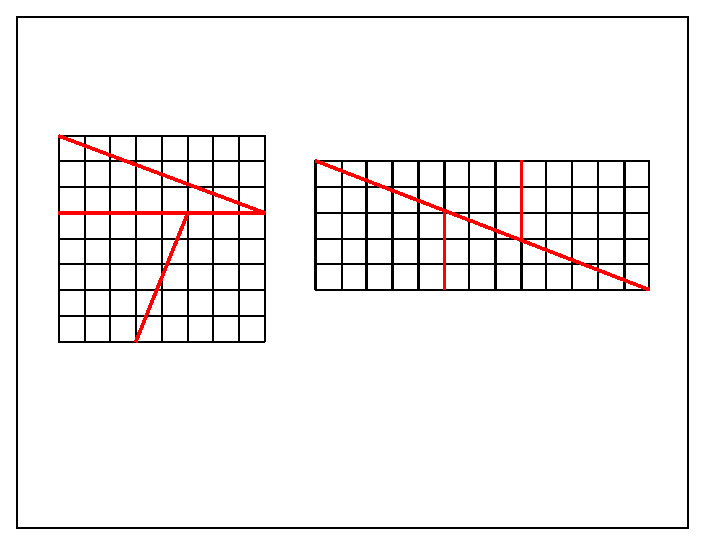
\includegraphics[width=\textwidth]{fibona}
Le carr\'e a comme surface 64 carr\'es alors que le rectangle est compos\'e de 
5*13=65 carr\'es. D'o\`u vient le carr\'e suppl\'ementaire ?
Le carr\'e suppl\'ementaire est l'aire du parall\'elogramme bleu !!!!\\

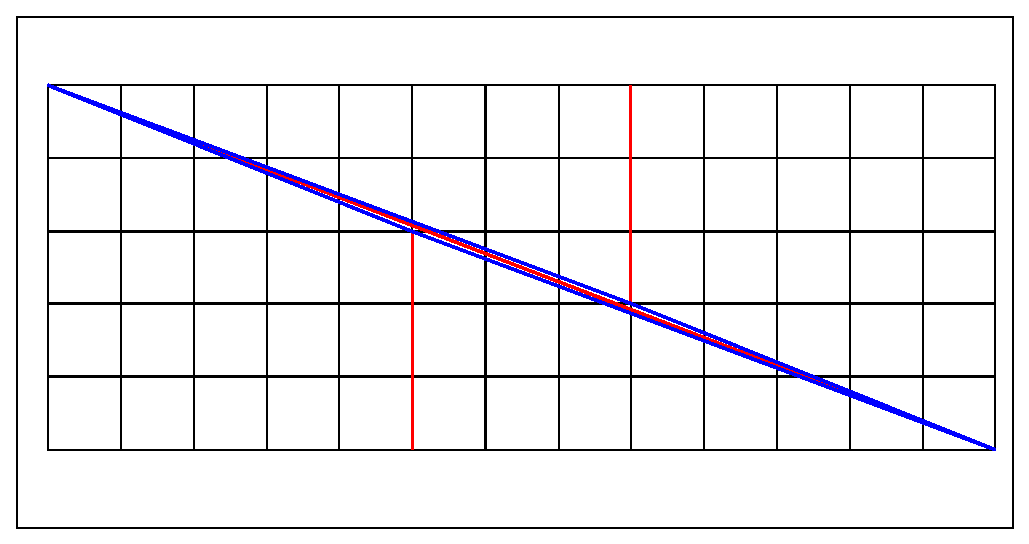
\includegraphics[width=\textwidth]{fibonac}

En effet les bords des 4 morceaux ne suivent pas la diagonale du rectangle qui
a comme pente $-5/13$ ce qui est diff\'erent de -2/5 et de -3/8.\\
Selon la longueur du carr\'e initial il peut soit y avoir un petit carr\'e en 
trop soit en manquer 1 puisque $u_{n+1}.u_{n-1}-u_n^2=(-1)^{n-1}$.


\section{La suite de Fibonacci et le triangle de Pascal}
\subsection{Le triangle de Pascal}
Pour avoir les premi\`eres valeurs du triangle de Pascal, on tape :\\
{\tt A:=makemat((j,k)->comb(j,k),11,11)}\\
On obtient :\\
$\left(\begin{array}{ccccccccccc}
1 & 0 & 0 & 0 & 0 & 0 & 0 & 0 & 0 & 0 & 0 \\
1 & 1 & 0 & 0 & 0 & 0 & 0 & 0 & 0 & 0 & 0 \\
1 & 2 & 1 & 0 & 0 & 0 & 0 & 0 & 0 & 0 & 0 \\
1 & 3 & 3 & 1 & 0 & 0 & 0 & 0 & 0 & 0 & 0 \\
1 & 4 & 6 & 4 & 1 & 0 & 0 & 0 & 0 & 0 & 0 \\
1 & 5 & 10 & 10 & 5 & 1 & 0 & 0 & 0 & 0 & 0 \\
1 & 6 & 15 & 20 & 15 & 6 & 1 & 0 & 0 & 0 & 0 \\
1 & 7 & 21 & 35 & 35 & 21 & 7 & 1 & 0 & 0 & 0 \\
1 & 8 & 28 & 56 & 70 & 56 & 28 & 8 & 1 & 0 & 0\\
1 & 9 & 36 & 84 & 126 & 126 & 84 & 36 & 9 & 1 & 0 \\
1 & 10 & 45 & 120 & 210 & 252 & 210 & 120 & 45 & 10 & 1
\end{array}\right) $\\
On peut aussi utiliser le tableur et la relation :\\
pour $n \in \N$ :
$C_n^0=1$, $C_n^n=1$ et  $C_n^p=C_{n-1}^p+C_{n-1}^{p-1}$ pour $0<p<n$.\\
On ouvre un niveau tableur et on choisit 22 lignes et 11 colonnes.\\
On met {\tt 1} dans $A0$.\\
Puis, on copie $A0$ vers le bas pour avoir des {\tt 1} dans la colonne $A$.\\
Dans $B1$ on met {\tt =B0+A0} formule que l'on copie vers le bas et vers la 
droite.\\
On copie alors vers le bas la formule situ\'ee dans $C1$,...$K1$.\\
{\bf Remarque} On peut mettre {\tt idn(11)} dans $A0$, et si on a 
coch\'e sur {\tt Distribuer}, cela a pour effet de remplir 11 lignes et 11 
colonnes avec la matrice identit\'e d'ordre 11. Mais cela est inutile car les 
1 de la diagonale sont recalcul\'es quand on copie vers la droite !\\
On obtient :\\
$\left(\begin{array}{ccccccccccc}
1 & 0 & 0 & 0 & 0 & 0 & 0 & 0 & 0 & 0 & 0 \\
1 & 1 & 0 & 0 & 0 & 0 & 0 & 0 & 0 & 0 & 0 \\
1 & 2 & 1 & 0 & 0 & 0 & 0 & 0 & 0 & 0 & 0 \\
1 & 3 & 3 & 1 & 0 & 0 & 0 & 0 & 0 & 0 & 0 \\
1 & 4 & 6 & 4 & 1 & 0 & 0 & 0 & 0 & 0 & 0 \\
1 & 5 & 10 & 10 & 5 & 1 & 0 & 0 & 0 & 0 & 0 \\
1 & 6 & 15 & 20 & 15 & 6 & 1 & 0 & 0 & 0 & 0 \\
1 & 7 & 21 & 35 & 35 & 21 & 7 & 1 & 0 & 0 & 0 \\
1 & 8 & 28 & 56 & 70 & 56 & 28 & 8 & 1 & 0 & 0\\
1 & 9 & 36 & 84 & 126 & 126 & 84 & 36 & 9 & 1 & 0 \\
1 & 10 & 45 & 120 & 210 & 252 & 210 & 120 & 45 & 10 & 1\\
1 & 11 & 55 & 165 & 330 & 462 & 462 & 330 & 165 & 55 & 11\\
1 & 12 & 66 & 220 & 495 & 792 & 924 & 792 & 495 & 220 & 66\\
1 & 13 & 78 & 286 & 715 & 1287 & 1716 & 1716 & 1287 & 715 & 286\\
1 & 14 & 91 & 364 & 1001 & 2002 & 3003 & 3432 & 3003 & 2002 & 1001\\
1 & 15 & 105 & 455 & 1365 & 3003 & 5005 & 6435 & 6435 & 5005 & 3003\\
1 & 16 & 120 & 560 & 1820 & 4368 & 8008 & 11440 & 12870 & 11440 & 8008\\
1 & 17 & 136 & 680 & 2380 & 6188 & 12376 & 19448 & 24310 & 24310 & 19448\\
1 & 18 & 153 & 816 & 3060 & 8568 & 18564 & 31824 & 43758 & 48620 & 43758\\
1 & 19 & 171 & 969 & 3876 & 11628 & 27132 & 50388 & 75582 & 92378 & 92378\\
1 & 20 & 190 & 1140 & 4845 & 15504 & 38760 & 77520 & 125970 & 167960 & 184756\\
1 & 21 & 210 & 1330 & 5985 & 20349 & 54264 & 116280 & 203490 & 293930 & 352716
\end{array}\right) $\\
On a ainsi les coefficients binomiaux utiles pour le d\'eveloppement de 
$(1+x)^n$ pour $n=0..21$.
\subsection{La somme des diagonales montantes}
Lorsqu'on fait la somme des diagonales montantes du triangle de Pascal on obtient la suite de Fibonacci.\\
Par exemple :\\
$\left(\begin{array}{cc}
1&=\\
&\\
1&=\\
&\\
2&=\\
&\\
3&=\\
&\\
5&=\\
&\\
8&=\\
&\\
13&=
\end{array}\right) $
$\left(\begin{array}{ccccccccccc}
1 & & 0 & &0 & &0 & &0 & &0 \\
 &\nearrow & &\nearrow &  &\nearrow &  & \nearrow &  &\nearrow  \\
1 & & 1 & &0 & &0 & &0 & &0 \\
 &\nearrow & &\nearrow &  &\nearrow &  & \nearrow &  &\nearrow  \\
1 & &2 & & 1 & &0 & &0 & &0 \\
&\nearrow & &\nearrow & &\nearrow &  &\nearrow  &  &  \\
1 & &3 & &3 & &1 & &0 & &0 \\
&\nearrow & &\nearrow & &\nearrow &  &  &  &  \\
1 & &4 & &6 & &4 & &1 & &0  \\
&\nearrow & &\nearrow & &&  & &  & \\
1 & &5 & &10 & &10 & &5 & &1 \\ 
&\nearrow & & & &&  & &  &  \\
1 & &6 & &15 & &20 & &15 & &6  
\end{array}\right) $\\
On tape :\\
{\tt L:=sum(A[j-k, k],k=0..j)\$(j=0..10)}\\
On obtient :\\
{\tt 1,1,2,3,5,8,13,21,34,55,89}\\
Pour le montrer on utilise les relations pour $n \in \N$ et $p \in \N$ :\\
$C_n^0=1$, $C_n^n=1$, $C_n^p=0$ si $p>n$ et  $C_n^p=C_{n-1}^p+C_{n-1}^{p-1}$ pour
 $0<p\leq n$.\\
On tape :\\
{\tt simplify(comb(j-1,k-1)+comb(j-1,k)-comb(j,k))}\\
On obtient :\\
{\tt 0}\\
Soit $a_n$ la suite d\'efinie par la somme des diagonales montantes du 
triangle de Pascal.\\
On a donc :\\
$a_0=1$, $a_1=1$ et pour $n>1$:\\
$a_n=\sum_{p=0}^{{\tt floor(n/2)}}{\tt comb(n-p,p)}=1+\sum_{p=1}^{{\tt floor(n/2)}}{\tt comb(n-p,p)}$\\ 
$a_n=1+\sum_{p=1}^{{\tt floor(n/2)}}{\tt comb(n-p-1,p-1)}+\sum_{p=1}^{{\tt floor(n/2)}}{\tt comb(n-p-1,p)}$\\
On a pour tout $n$ : ${\tt floor(n/2)-1=floor((n-2)/2))}$.\\
On a si  $n=2k$, on a ${\tt floor(n/2)=floor((n-1)/2)+1}=k$:\\
$1+\sum_{p=1}^{{\tt floor(n/2)}}{\tt comb(n-p-1,p)}=$\\
$\sum_{p=0}^{{\tt floor((n-1)/2)}}{\tt comb(n-1-p,p)}+{\tt comb(2k-1-k,k)}=a_{n-1}$\\ 
car ${\tt comb(2k-1-k,k)}=0$\\
$\sum_{p=1}^{{\tt floor(n/2)}}{\tt comb(n-p-1,p-1)}=$\\
$\sum_{p=0}^{{\tt floor((n-2)/2)}}{\tt comb(n-2-p,p)}=a_{n-2}$\\ 
car {\tt floor(n/2)-1=floor((n-2)/2)}\\
On a si  $n=2k+1$ alors ${\tt floor(n/2)=floor((n-1)/2)=k}$ :\\
$1+\sum_{p=1}^{{\tt floor(n/2)}}{\tt comb(n-p-1,p)}=$\\
$\sum_{p=0}^{{\tt floor((n-1)/2)}}{\tt comb(n-1-p,p)}=a_{n-1}$\\
$\sum_{p=1}^{{\tt floor(n/2)}}{\tt comb(n-p-1,p-1)}=$\\
$\sum_{p=0}^{{\tt floor((n-2)/2)}}{\tt comb(n-2-p,p)}=a_{n-2}$ \\
car {\tt floor(n/2)-1=floor((n-2)/2)}\\
Donc :\\
$a_0=1$, $a_1=1$ et pour $n>1$ on a
$a_n=a_{n-1}+a_{n-2}$\\
$a_n$ est donc la suite de Fibonacci.\\
On tape :\\
{\tt L1:=0,sum(A[j-k-1,k-1],k=1..j-1)\$(j=1..10)}\\
On obtient :\\
{\tt 0,0,1,1,2,3,5,8,13,21,34}\\
On tape :\\
{\tt L2:=1,sum(A[j-k-1,k],k=0..j-1)\$(j=1..10)}\\
On obtient :\\
{\tt 1,1,1,2,3,5,8,13,21,34,55}\\
On tape :\\
{\tt [L1]+[L2]}\\
On obtient :\\
{\tt [1,1,2,3,5,8,13,21,34,55,89]}\\
On tape :\\
{\tt simplify(comb(j-1,k-1)+comb(j-1,k)-comb(j,k))}\\
On obtient :\\
{\tt 0}
\section{Le code de Fibonacci}
\`A partir de "sa" suite Fibonacci a fabriqu\'e un code qui permet d'\'ecrire 
tous les entiers avec des 0 et des 1. Pour cela, si $u_n$ est la suite de 
Fibonacci  $u_0=u_1=1$ et pour $n\geq2$ $u_n=u_{n-2}+u_{n-1}$,
le code de 0 est 0 et pour $n>0$ le code des nombres $u_n$ est 1 suivi de $n-1$ z\'eros.\\
On a ainsi :\\
0 a pour code 0\\
1 a pour code 1\\
2 a pour code 10\\
3 a pour code 100\\
4 a pour code 101 car 4=3+1\\
5 a pour code 1000\\
6 a pour code 1001 car 6=5+1\\
7 a pour code 1010 car 7=5+2\\
8 a pour code 10000\\
etc...\\
On remarquera que dans ce code il n'y a jamais deux 1 qui se suivent, en effet :\\ 
$u_{n-1}+u_{n-2}=u_n$. \\
Par exemple le nombre :\\
$u_1+u_2+u_3+u_4=1+2+3+5=11$ a comme code 1010 car 11=8+3.\\
{\bf Exercice}\\
\'Ecrire un programme qui renvoie le code de Fibonacci d'un entier $n\geq 10^8$.\\
On remarquera que $u_{38}<10^8<u_{39}$.\\
On construit la liste des 40 premiers termes de $u_n$ pour $n=0,1..39$.\\
{\bf Le codage}\\
On utilise le programme vu pr\'ec\'edemment :
\begin{verbatim}
Fibonasuite(n):={
local a,b,c,L;
L:=NULL;
si n<=0 alors retourne L;fsi;
L:=L,1;
si n==1 alors retourne L;fsi;
L:=L,1;
si n==2 alors retourne L; fsi;
a:=1;
b:=1;
pour k de 3 jusque n faire
    c:=a+b;
    L:=L,c;
    a:=b;
    b:=c;
fpour;
retourne L;   
}:;
\end{verbatim}
On \'ecrit  le code d'un nombre $n$ au moyen d'une chaîne de caract\`eres : 
c'est {\tt string} qui transforme l'\'ecriture d'un nombre en une chaîne
de caract\`eres 
\begin{verbatim}
codefib(n):={
local fib,cod,p;
si n>10^8 alors retourne "l'entier doit etre <10^8" fsi;
si (n==0 or n==1) alors  return n fsi;
fib:=Fibonasuite(40);
cod:=0;
repeter
p:=2;
tantque n>=fib[p] faire p:=p+1 ftantque;
// fib[p-1]<=n<fib[p]
cod:=10^(p-2)+cod;
n:=n-fib[p-1];
jusqua n==0;
retourne string(cod);
}:;
\end{verbatim}
On tape :\\
{\tt codefib(n)\$(n=0..20)}\\
On obtient une suite de chaînes :\\
{\tt 0,1,10,100,101,1000,1001,1010,10000,10001,10010,10100,10101,}\\
{\tt 100000,100001,100010,100100,100101,101000,101001,101010}\\
{\bf Le d\'ecodage}\\
On donne une chaîne de caract\`eres $L$ de 1 et de z\'ero qui est le code de 
Fibonacci d'un nombre $n$ et on obtient le nombre $n$ cod\'e par $L$.\\
On remarquera que le d\'ecodage ci-dessous ne v\'erifie pas que $L$ est bien un
code de Fobonacci : il peut y avoir 2 "1" \`a la suite (par ex decodefib("11") 
renverra 3) et les chiffres autres que "1" seront consid\'er\'es comme des "0"
(par ex decodefib("15") renverra 2).\\
On tape :
\begin{verbatim}
decodefib(L):={
local k,n,s,fib;
fib:=Fibonasuite(40);
s:=dim(L);
si s==1 alors return expr(L[0]); fsi; 
n:=0;
pour k de 0 jusque s-1 faire
si L[k]=="1" alors n:=n+fib[s-k];fsi; 
fpour;
return n;
}:;
\end{verbatim}
On tape :\\
{\tt decodefib("101010"),decodefib("10101")}\\
On obtient :\\
{\tt 20,12}
\section{Le nombre d'or}
Les quotients des termes successifs de la suite de Fibonnacci est la suite 
$v_n=\frac{u_{n+1}}{u_n}$  pour $n \geq 0$\\
Cette suite converge vers  
$\frac{1+\sqrt 5}{2}$ : c'est le nombre d'or  qui est not\'e $\Phi$.\\
En effet, on a $v_0=1$ et $v_n=1+\frac{u_{n-1}}{u_n}=1+\frac{1}{v_{n-1}}$ donc \\
$v_1=2$, $v_2=3/2$, $v_3=5/3$.\\
Montrons par re\'ecurrence que $1 \leq v_n \leq 2$ pour tout $n$ :
$1\leq v_0=1<2$
si $1 \leq v_{n-1}<2$ alors $1/2\leq \frac{1}{v_{n-1}}\leq 1$
donc $1\leq 1+1/2 \leq v_n\leq 1+1=2$\\
\'Etude du signe de $v_n-v_{n-1}$ :\\
$v_n-v_{n-1}=\frac{1}{v_{n-1}}-\frac{1}{v_{n-2}}=\frac{v_{n-2}-v_{n-1}}{v_{n-1}v_{n-2}}$\\
Donc $v_n-v_{n-1}$ est du signe oppos\'e \`a celui de $v_{n-1}-v_{n-2}$.\\
Donc $v_{2n}-v_{2n-2}$ a le m\^me signe que $v_2-v_0=1/2>0$ et\\
$v_{2n+1}-v_{2n-1}$ a le m\^eme signe que $v_3-v_1=-1/3<0$\\
La suite $v_{2n}$ est convergente vers $1\leq a\leq 2$ car croissante et 
major\'ee.\\
$v_{2n+1}$ est convergente vers $1\leq b\leq 2$ car d\'ecroissante et 
minor\'ee.\\
On doit avoir $a=1+1/b$ et $b=1+1/a$ donc $ab=b+1=a+1$ donc $a=b$
Donc $v$ converge vers $a=b=\phi$ qui v\'erifie :\\
$\phi=1+\frac{1}{\phi}$ ou encore $\phi^2-\phi-1=0$ et $1\leq \phi \leq 2$.
donc $\phi=\frac{1+\sqrt 5}{2}$
Le nombre d'or est :
$$\phi=\frac{1+\sqrt 5}{2}\simeq 1.61803398875$$
\subsection{Propri\'et\'es du  nombre d'or}
$$\phi^2=1+\phi$$
$$(\phi-1)*\phi=1$$
$$\phi=\sqrt{1+\sqrt{1+\sqrt{1+\sqrt{1+...}}}}$$ 
$$ \frac{1}{\phi}=1+\phi$$
$$ \phi=1+\frac{1}{1+\displaystyle\frac{1}{1+\displaystyle\frac{1}{1+...}}}$$
Si un r\'ectangle est tel que le rapport de la longueur $L$ \`a la largeur $l$ 
soit $\phi$ alors :
$$\frac{L}{l}=\frac{l}{L-l}=\phi$$
On tape :
\begin{verbatim}
spiror(a,b,n):={
local au,r,L;
L:=NULL;
si n==0 alors retourne L,segment(a,b);fsi;
au :=(1+sqrt(5))/2;
L:=L,rectangle(a,b,au-1);
r:=(b-a)*(au-1);
L:=L,affichage(cercle(a+r,r,pi/2,pi),1);
retourne L,spiror(a+r*(1+i),a+r,n-1);
}:;
\end{verbatim}
puis on tape :\\
{\tt spiror(0,1/2+sqrt(5)/2,7)}\\
On obtient :\\

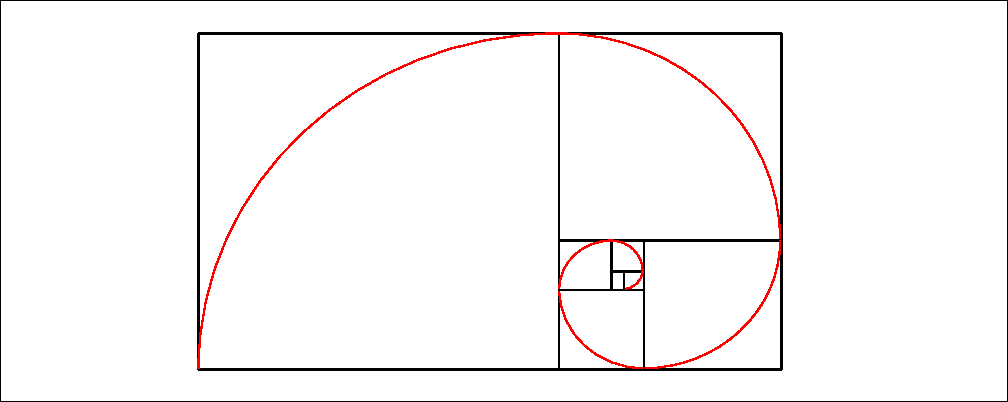
\includegraphics[width=\textwidth]{fibonspi}
\section{Un exercice niveau trousi\`eme}
On veut construire un rectangle d'or i.e. un rectangle tel que :\\
longueur/largeur =$\frac{1+\sqrt 5}{2}=\Phi$.\\
Tout d'abord \'etant donn\'e un segment $AB$, on construit un point $M$ tel que
$\frac{AB}{MB}=\frac{MB}{MA}=\frac{1+\sqrt 5}{2}=\Phi$\\
Soient $a$ un nombre r\'eel positif et $ABC$ un triangle rectangle en $A$ tel 
que $AB=a$ et $AC=a/2$.\\
Soit $N$ intersection du cercle de centre $C$ et de rayon $AC$.\\
Soit $M$ intersection du cercle de centre $B$ et de rayon $BN$.\\
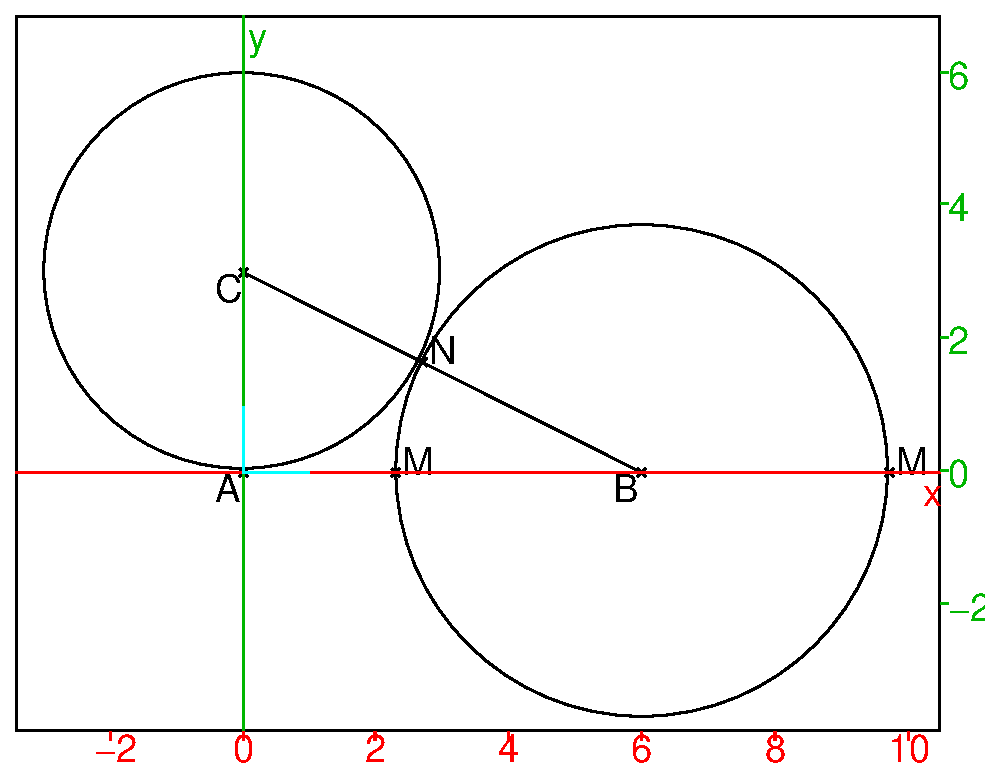
\includegraphics[width=\textwidth]{fibonap}\\
Calculer les longueurs $BC$, $BN$, $BM$ et $AM$.\\
Montrer que $M$ partage $BA$ selon le nombre d'or i.e. :
$$\frac{MB}{MA}=\frac{AB}{MB}=\frac{1+\sqrt 5}{2}=\Phi$$
En d\'eduire une construction d'un rectangle d'or avec {\tt Xcas}\\
{\bf Solution}\\
D'apr\`es le th\'eor\`eme de Phytagore on a :\\
$BC^2=AB^2+AC^2=a^2+a^2/4=5a^2/4$\\
Donc :\\
$\displaystyle BC=\frac{a\sqrt 5}{2}$\\
$\displaystyle BN=BM=BC-CN=BC-a/2=\frac{a(\sqrt 5-1}{2}$\\
$\displaystyle AM=AB-BM=a-\frac{a(\sqrt 5-1}{2}=\frac{a(3-\sqrt 5}{2}$\\
On a donc :
$$\frac{MB}{MA}=\frac{\sqrt 5-1}{3-\sqrt 5}=\frac{1+\sqrt 5}{2}=\Phi$$
$$\frac{AB}{MB}=\frac{2}{\sqrt 5-1}=\frac{1+\sqrt 5}{2}=\Phi$$
{\bf Remarque}\\
On peut se servir de {\tt Xcas} pour faire les calculs.\\
On peut stocker les valeurs dans des variables.
On tape :\\
{\tt a\verb|^|2+a\verb|^|2/4}\\
On obtient $BC^2$ :\\
{\tt 5*a\verb|^|2/4}\\
On tape :\\
{\tt factor(sqrt(5*a\verb|^|2/4))}\\
On obtient $BC$ :\\
{\tt sqrt(5)*a/2}\\
On tape :\\
{\tt factor(a*sqrt(5)/2-a/2)}\\
On obtient $CN$ et $BM$ :\\
{\tt (sqrt(5)-1)*a/2}\\
On tape :\\
{\tt factor(a-(sqrt(5)-1)*a/2)}\\
On obtient $AM$ :\\
{\tt (-(sqrt(5))+3)*a/2}\\
On tape :\\
{\tt normal((sqrt(5)-1)*a/2/((-(sqrt(5))+3)*a/2))}\\
On obtient $BM/AM$ :\\
{\tt (sqrt(5)+1)/2}\\
On tape :\\
{\tt normal(a/((sqrt(5)-1)*a/2))}\\
On obtient $AB/BM$ :\\
{\tt (sqrt(5)+1)/2}.\\
On peut stocker les valeurs dans des variables pour que les calculs soient plus
 lisibles.\\
On tape :\\
{\tt BC:=factor(sqrt(a\verb|^|2+a\verb|^|2/4))}\\
On obtient $BC$ :\\
{\tt sqrt(5)*a/2}\\
On tape :\\
{\tt BM:=factor(BC-a/2)}\\
On obtient $CN$ et $BM$ :\\
{\tt a*(sqrt(5)-1)/2}\\
On tape :\\
{\tt AM:=factor(a-BM)}\\
On obtient $AM$ :\\
{\tt a*(-(sqrt(5))+3)/2}\\
On tape :\\
{\tt normal(BM/AM)}\\
On obtient $BM/AM$ :\\
{\tt (sqrt(5)+1)/2}\\
On tape :\\
{\tt normal(a/BM)}\\
On obtient $AB/BM$ :\\
{\tt (sqrt(5)+1)/2}.\\
{\bf Construction du rectangle d'or}
\begin{verbatim}
A:=point(0);
B:=point(4);
K:=point(0,2,affichage=3);
triangle(A,B,K,affichage=3);
cercle(K,2,affichage=3);
N:=inter(cercle(K,2),segment(K,B));
l:=longueur(K,B);
cercle(B,l-2,affichage=3);
M:=inter(cercle(B,l-2),segment(A,B));
rectangle(A,B,(l-2)/4,D,C);
L:=point(6-l,l-2);
segment(M,L);
\end{verbatim}
On obtient :\\
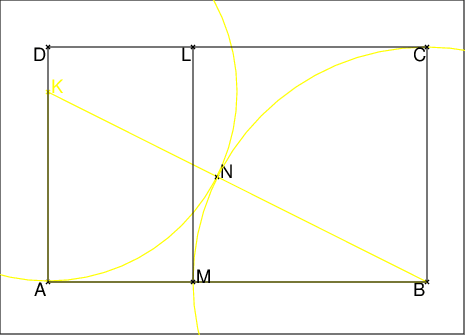
\includegraphics[width=\textwidth]{fibonarect}\\
Les rectangles $ABCD$ et $AMLD$ sont des rectangles d'or et $MBCL$ est un 
carr\'e.
\section{Un exercice niveau terminale}
\subsection{L'\'enonc\'e}
On cosid\`ere la fonction $f$ definie sur $\R^*$ par :
$$f(x)=\frac{x+1}{x}$$
On note $f@@ n=f\circ f..\circ f\ $ (On compose $f$, $n$ fois)
\begin{enumerate}
\item Calculer :
$f@@ 2=f\circ f,\hspace*{0.5cm} f@@ 3=f\circ f\circ f,\hspace*{0.5cm} f@@ 4=f\circ f\circ f\circ f$
\item Trouver la valeur de $f@@ n$ en fonction de $n$.
\item R\'esoudre, lorsqu'on utilise $n$ traits de fractions, l'\'equation 
d'inconnue $x$ :
$$x=1+\frac{1}{1+\displaystyle\frac{1}{1+\displaystyle\frac{1}{1+\displaystyle\frac{1}{...+\displaystyle\frac{1}{1+\displaystyle\frac{1}{x}}}}}}$$
\item Touver la limite lorsque $n$ tends vers $+\infty$ de
 $$1+\frac{1}{1+\displaystyle\frac{1}{1+\displaystyle\frac{1}{1+\displaystyle\frac{1}{...+\displaystyle\frac{1}{1+\displaystyle\frac{1}{a}}}}}}$$
lorsque $a>0$ et lorsqu'on utilise $n$ traits de fractions.
\end{enumerate}
\subsection{La solution avec {\tt Xcas}}
\begin{enumerate}
\item On d\'efinit la fonction $f$, on tape :\\
{\tt f(x):=(x+1)/x}\\
On calcule $f@@ 2=f(f(x))$, on tape :\\
{\tt normal((f@@2)(x))}\\
On obtient :\\
{\tt (2*x+1)/(x+1)}\\
 On calcule $f@@ 3=f(f(f(x)))$, on tape :\\
{\tt normal((f@@3)(x))}\\
On obtient :\\
{\tt (3*x+2)/(2*x+1)}\\
On calcule $f@@ 4$, on tape :\\
{\tt normal((f@@4)(x))}\\
On obtient :\\
{\tt (5*x+3)/(3*x+2)}\\
\item On suppose que :
$\displaystyle f@@ n=\frac{a_nx+b_n}{c_nx+d_n}$\\
On cherche une relation de r\'ecurrence entre les diff\'erents coefficients.\\
On d\'efinit la fonction $g$, on tape :\\
{\tt g(x,a,b,c,d):=(a*x+b)/(c*x+d)}\\
On a :
$(f@@ n+1)(x)=f(g(x,a,b,c,d))$\\
 On calcule $f(g(x,a,b,c,d))$ et on tape :\\
{\tt normal(f(g(x,a,b,c,d)))}\\
On obtient :\\
{\tt (a*x+b+c*x+d)/(a*x+b)}\\
donc :\\
$c_{n+1}=a_n$,\hspace*{0.5cm}$d_{n+1}=b_n$\\
$a_{n+1}=a_n+c_n=a_n+a_{n-1}$\\
$b_{n+1}=b_n+d_n=b_n+b_{n-1}$\\
On sait que $a_1=1,\ b_1=1\ a_0=c_1=1\ b_0=d_1=0$\\
Donc si la suite de Fibonacci est la suite $u$ d\'efinie par :\\
$u_0=1$,\hspace*{0.5cm} $u_1=1$\\
$u_n=u_{n-1}+u_{n-2}$ pour $n>1$:\\
Alors 
$\displaystyle f@@ n=\frac{a_nx+b_n}{c_nx+d_n}$
avec $a_n=u_n,\ b_n=c_n=a_{n-1},\ d_n=a_{n-2}$
\item On r\'esout l'\'equation d'inconnue $x$, avec 1 trait de fractions :
$\displaystyle x=1+\frac{1}{x}$\\
On tape :\\
{\tt normal(1+1/x)}\\
On obtient : {\tt (x+1)/x}\\
Donc $\displaystyle f(x)=1+\frac{1}{x}$\\
Il faut donc r\'esoudre $f(x)=x$, on tape :\\
{\tt solve(x=f(x),x)}\\
On obtient : {\tt [1/2*(1-sqrt(5)),1/2*(1+sqrt(5))]}\\
On reconnait le nombre d'or et l'inverse de son oppos\'e.\\
On r\'esout l'\'equation d'inconnue $x$, avec 2 traits de fractions :
$x=1+\displaystyle \frac{1}{1+\displaystyle \frac{1}{x}}$\\
On tape :\\
{\tt normal(1+1/(1+1/x))}\\
On obtient : {\tt (2*x+1)/(x+1)}\\
On reconnait $f(f(x))$ ou bien 
puisque $\displaystyle f(x)=1+\frac{1}{x}$, on a :\\
$1+\displaystyle \frac{1}{1+\displaystyle \frac{1}{x}}=1+\frac{1}{f(x)}=f(f(x))$\\. 
Il faut donc r\'esoudre $f(f(x))=x$, on tape :\\
{\tt solve(f(f(x))=x,x)}\\
On obtient :
{\tt [1/2*(1-sqrt(5)),1/2*(1+sqrt(5))]}\\
qui sont les m\^emes solutions qur $f(x)=x$. \\
On doit r\'esoudre l'\'equation avec $n$ traits de fractions :
$(f@@ n)(x)=x$\\
Comme $(f@@ n)$ est une fonction homographique (i.e.
$(f@@ n)(x)$ est de la forme $(a*x+b)/(c*x+d))$),
cette \'equation est une \'equation du 2-nd degr\'e donc admet au plus 2 
solutions. Les 2 solutions de $f(x)=x$ sont aussi solutions de
$(f@@ n)(x)=x$ donc $(f@@ n)(x)=x$  a les m\^emes solutions que
$f(x)=x$.
\item Chercher la limite lorsque le nombre de traits tend vers l'infini de :
$$1+\frac{1}{1+\displaystyle\frac{1}{1+\displaystyle\frac{1}{1+\displaystyle\frac{1}{...\frac{1}{1+\displaystyle\frac{1}{a}}}}}}$$
revient \`a chercher la limite de la suite des it\'er\'ees de $f$ d\'efinit 
par : $u_0=a>0,\ u_n=f(u_{n-1})$ pour $n>0$.
On a en effet (avec $n$ traits de fractions) :
$$u_n=1+\frac{1}{1+\displaystyle\frac{1}{1+\displaystyle\frac{1}{1+\displaystyle\frac{1}{...\frac{1}{1+\displaystyle\frac{1}{a}}}}}}$$.
Avec {\tt Xcas}, on tape dans un niveau de g\'eom\'etrie 2-d :\\
{\tt supposons(a=[6.0,0,9,0.1])}\\
{\tt plotseq(1+1/x,[a,0,9],5)}\\ 
On obtient :\\
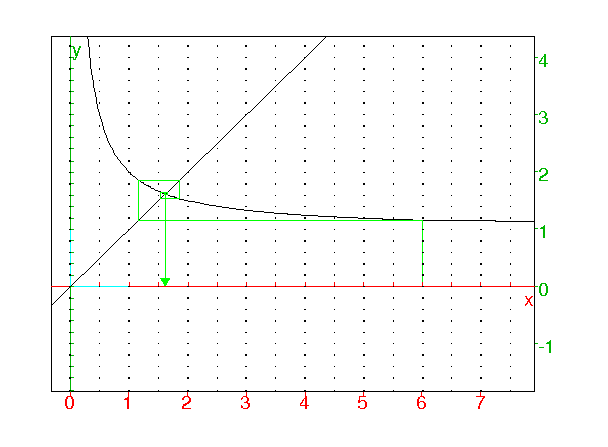
\includegraphics[width=\textwidth]{fiboniter}
Montrons que la suite $u_n$ converge vers 
$\phi=\frac{1+\sqrt5}{2}$ qui est la 
solution positive de l'\'equation $f(x)=x$.\\
Puisque $a>0$, on a $u_1=b=1+1/a>1>0$ et pour tout $n>0$ $u_n>1>0$.\\
Si $u_0=a>\phi$ alors $b=u_1=1+1/a<1+1/\phi=\phi$ et \\
si $u_0=a<\phi$ alors $b=u_1=1+1/a>1+1/\phi=\phi$
De m\^eme si $c=u_n>\phi$ alors $d=u_{n+1}=1+1/c<\phi$ et $u_{n+2}=1+1/c>\phi$.\\
Suupposons par exemple que $a=u_0>\phi$ \\ 
Alors pour tout $n\in \N$ on a $u_{2n}>\phi$ et $u_{2n+1}<\phi$\\
On a :\\
$u_{n+1}-u_n=f(u_n)-f(u_{n-1})=1/u_n-1/u_{n-1}=(u_{n-1}-u_n)/(u_{n-1}u_n)$\\
Comme $(u_{n-1}u_n)>0$ on en d\'eduit que $u_{n+1}-u_n$ et $u_n-u_{n-1}-$
sont de signe oppos\'e donc que $u_{n+1}-u_n$ et $u_{n-1}-u_{n-2}$ et  sont de 
m\^eme signe.\\
Ainsi $u_{2n}-u_{2n-2}$ a le m\^eme signe que  $u_2-u_0$ et\\
$u_{2n+1}-u_{2n-1}$ a le m\^eme signe que  $u_3-u_1$.\\
Signe de $u_2-u_0$ :\\
$u_2-u_0=(2a+1)/(a+1)-a=(-a^2+a+1)/(a+1)<0$ puisque $a>\phi$ et que $\phi$ est la 
plus grande racine de  $-x^2+x+1$\\
Signe de $u_3-u_1$ :\\
$u_3-u_1=(2b+1)/(b+1)-b=(-b^2+b+1)/(b+1)>0$ puisque $0<b<\phi$ et que $\phi$ est la 
plus grande racine de  $-x^2+x+1$ et que 0 se trouve entre les racines.\\
On a donc montrer que $u_{2n}$ est d\'ecroissante et minor\'ee donc est 
convergente vers la solution positive de $f(f(x))=x$ qui est $\phi$ 
et que $u_{2n+1}$ est croissante et major\'ee donc est convergente
vers la solution positive de $f(f(x))=x$ qui est $\phi$ .
Donc $u_n$ converge vers $\phi$.\\
{\bf Remarque} Lorsque $a=1$, $u_n$ est le quotient de de 2 termes cons\'ecutifs
de la suite de Fibonacci.
\end{enumerate}
\section{Deux suites convergentes vers le nombre d'or $L$} 
\subsection{$u_0=1$ et $u_{n+1}=\sqrt{1+u_n}$ pour $n\in \N$}
Soit la suite $u$ d\'efinie par :\\
$u_0=1$ et $u_{n+1}=\sqrt{1+u_n}$ pour $n\in \N$.\\
Calculer une valeur approch\'e de $u_5$.\\
Montrer que $u$ est \`a terme positif et est croissante (on montrera que
$u_{n+1}-u_n>0 $ pour $n\in \N$).\\
Soit $L$ la racine positive de $x^2-x-1=0$. \\
Montrer que $u_n<L$ pour $n\in \N$.\\
En d\'eduire que $u$ converge vers $\displaystyle L=\frac{1+\sqrt 5}{2}$\\
On tape :\\
{\tt sqrt(1+sqrt(1+sqrt(1+sqrt(1+sqrt(2.)))))}\\
On obtient :\\
{\tt 1.61612120651}\\
ou bien, on tape :\\
{\tt 1}\\
{\tt sqrt(1.+ans())}\\
On valide la derni\`ere ligne 5 fois et on obtient :\\
{\tt 1.61612120651}\\
ou bien, on utilise le tableur...\\
On tape :\\
{\tt mult\_conjugate(sqrt(1+u1)-sqrt(1+u0))}\\
On obtient apres simplification du num\'erateur :\\
{\tt (-u0+u1)/(sqrt(1+u1)+sqrt(1+u0))}\\
ce qui veut dire que $u_2-u_1$ a la m\^eme signe que $u_1-u_0=\sqrt 2-1>0$.\\
Le m\^eme calcul montre que $u_{n+1}-u_n$ a la m\^eme signe que $u_n-u_{n-1}$ qui
a la m\^eme signe que $u_{n-1}-u_{n-2}$ etc..qui a la m\^eme signe que 
$u_1-u_0$.\\
Donc $u_{n+1}-u_n>0$ pour $n\in \N$. La suite $u$ est donc croissante.\\
On tape :\\
{\tt solve(x\verb|^|2-x-1)}\\
On obtient :\\
{\tt [1/2*(1-(sqrt(5))),1/2*(1+sqrt(5))]}\\
Donc $L=1/2*(1+\sqrt 5)\simeq 1.61803398875$ et $L=\sqrt{1+L}$.\\
On tape :\\
{\tt mult\_conjugate(sqrt(1+un)-sqrt(1+L))}\\
On obtient :\\
{\tt (-L+un)/(sqrt(1+un)+sqrt(1+L))}\\
Donc $u_{n+1}-L$ a le m\^eme signe que $u_n-L$ qui
a la m\^eme signe que $u_{n-1}-L$ etc..qui a la m\^eme signe que 
$u_0-L=1/2*(1-sqrt(5))<0$. Donc $u$ est major\'ee par $L$.\\
La suite $u$ est croissante et major\''e donc $u$ est convergente et sa limite 
$a$ v\'erifie $a=\sqrt{1+a}$. Donc $a=L$.\\
La  convergence de $u_n$ n'est pas tr\`es rapide puisque $u_5$ donne la 
valeur de $L$ avec seulement 2 d\'ecimales exactes.

\subsection{$u_0=2$ et $u_{n+1}=\frac{u_n^2+1}{2u_n-1}$ pour $n\in \N$} 
Soit la suite $u$ d\'efinie par :\\
$u_0=2$ et $u_{n+1}=\frac{u_n^2+1}{2u_n-1}$ pour $n\in \N$.\\
En consid\'erant la fonction $g$ d\'efinie par $g(x)=x^2-x-1$, montrer que 
$u_n$ est la suite de la m\'ethode de Newton pour trouver une valeur 
approch\'ee de {\tt L:=1/2*(1+sqrt(5))} qui est le z\'ero de $g$ dans
$[1,2]$, c'est \`a dire que $u_{n+1}=u_n-\frac{g(u_n}{g'(u_n)}$.\\
Montrer que $u_{n+1}-L=\frac{(u_n-L)^2}{2u_n-1}$.\\
Montrer par r\'ecurrence que $u_n>L$ pour tout $n\in \N$\\
Montrer que $u$ est d\'ecroissante et converge vers $L$\\
Calculer une valeur approch\'e de $u_5$.\\
On tape :\\
{\tt g(x):=x\verb|^|2-x-1}\\
{\tt f(x):=x-g(x)/g'(x)}\\
{\tt normal(f(x))}\\
On obtient :
{\tt  (x\verb|^|2+1)/(2*x-1)}\\
Donc $u_{n+1}=f(u_n)$.\\
On tape :\\
{\tt L:=1/2*(1+sqrt(5))}\\
{\tt normal(f(L))}\\
On obtient :
{\tt 1/2*(1+sqrt(5))}\\
Donc $f(L)=L$
On tape pour calculer $u_{n+1}-L$:\\
{\tt factor(f(un)-f(L))}\\
On obtient :\\
{\tt (2*(un+(-(sqrt(5))-1)/2)\verb|^|2)/(4*un-2)}\\
On a $u_0=2>L$ et si $u_n>L$ alors $2u_n-1>2L-1>0$ donc puisque
$u_{n+1}-L=\frac{(u_n-L)^2}{2u_n-1}>0$ on en d\'eduit que $u_{n+1}>L$.\\
On tape pour avoir le signe de $u_{n+1}-u_n$ :\\
{\tt normal(f(un)-un)}\\
On obtient :
{\tt (-un\verb|^|2+un+1)/(2*un-1)}\\
Comme $u_n>L$ $u_n$ est \`a l'ext\'erieur des racines de $-x^2+x+1$ donc 
$-u_n^2+u_n+1<0$ et $2u_n-1>0$ donc $u_{n+1}-u_n<0$ donc $u$ est d\'ecroissante 
et converge vers $a$ la racine positive de $f(x)-x$.\\
On tape :\\
{\tt normal(solve(f(x)-x))}\\
On obtient :
{\tt [(-(sqrt(5))+1)/2,(sqrt(5)+1)/2]}\\
Donc $a=L=(\sqrt 5+1)/2$\\
On tape :\\
{\tt (f@@5)(2.)}\\
On obtient (avec 30 chiffres significatifs):\\
{\tt 1.618033988749894848204586838338}\\
On tape :\\
{\tt (f@@5)(2.)-(sqrt(5)+1)/2.}\\
On obtient :\\
{\tt 0.3972703518693015452053465054764e-26}\\
La  convergence de $u_n$ est tres rapide puisque $u_5$ donne la valeur de $L$ 
avec 26 d\'ecimales exactes.
\section{Le nombre d'or et $\cos(\frac{\pi}{5})$}
\subsection{Calcul de $\cos(\frac{2\pi}{5})$}
Soit $\displaystyle z_1=\exp(i*\frac{2\pi}{5})$. \\
$\displaystyle z_1=a+ib=\cos(\frac{2\pi}{5})+i*\sin(\frac{2\pi}{5})$ est la racine de 
$z^5-1=0$ qui v\'erifie $a>0$ et $b>0$.\\
Puisque $z^5-1=(z-1)(z^4+z^3+z^2+z+1)$, $z_1=a+ib$ est la racine de 
$z^4+z^3+z^2+z+1=(z+\frac{1}{z})^2+(z+\frac{1}{z})-1=0$.\\
On pose $\displaystyle Z=z+\frac{1}{z}$ et on tape :\\
{\tt solve(Z\verb|^|2+Z-1,Z)}\\
On obtient :
{\tt [1/2*(-1-sqrt(5)),1/2*(-1+sqrt(5))]}\\
Comme $z_1=a+ib$ est de module 1, on a  $\frac{1}{z1}=a-ib$ et donc 
$z1+\frac{1}{z1}=2a=2\cos(\frac{2\pi}{5})$.\\
On a donc :
$$\cos(\frac{2\pi}{5})=\frac{-1+\sqrt 5}{4}$$
On tape :\\
{\tt normal(expand((1/4*(-1+sqrt(5)))\verb|^|2))}\\
On obtient :
{\tt (-sqrt(5)+3)/8}\\
Donc :
$$\cos(\frac{2\pi}{5})^2=\frac{3-\sqrt 5}{8}$$
$$\sin(\frac{2\pi}{5})^2=\frac{5\sqrt 5}{8}$$
\subsection{Calcul de $2\cos(\frac{\pi}{5})$}
On a :
$\displaystyle \cos(\frac{2\pi}{5})=2\cos(\frac{\pi}{5})^2-1$\\
Donc :\\
$2\cos(\frac{\pi}{5})^2=\cos(\frac{2\pi}{5})+1)=\frac{-1+\sqrt 5}{4}+1$\\
On tape :
{\tt normal(1/4*(-1+sqrt(5))+1)}\\
On obtient :
{\tt (sqrt(5)+3)/4}\\
Donc :
$$\cos(\frac{\pi}{5})^2=\frac{3-\sqrt 5}{8}$$
On tape :
{\tt normal(expand((1/4*(1+sqrt(5)))\verb|^|2))}\\
On obtient :
{\tt (sqrt(5)+3)/8}\\
Donc :
$$\cos(\frac{\pi}{5})=\frac{1+\sqrt 5}{4}$$
Le nombre d'or est :
$$\phi=\frac{1+\sqrt 5}{2}\simeq 1.61803398875$$
Donc $$2\cos(\frac{\pi}{5})=\phi$$
\chapter{Les fractions continues et $\pi$}
\section{D\'eveloppement en fractions continues de $\pi$}
Avec {\tt Xcas} si on tape :\\
{\tt evalf(pi,21)}\\
On obtient :\\
{\tt 3.141592653589793238462}\\
Une valeur approch\'ee par exc\`es de $\pi$ par un rationnel est : 
$$\frac{22}{7}$$
On a $\frac{22}{7}\simeq 3.14285714286$ ce qui fait 2 d\'ecimales exactes et\\
{\tt evalf(22/7-pi)} renvoie {\tt 0.00126448926721}\\
Donc $0<\frac{22}{7}-0.0013<\pi<\frac{22}{7}$ et $0<\frac{22}{7}-\pi<1.310^{-3}$\\

Une autre valeur approch\'ee par exc\`es de $\pi$ par un rationnel est : 
$$\frac{355}{113}$$
On a $\frac{355}{113}\simeq 3.14159292035$ ce qui fait 6 d\'ecimales exactes et\\
{\tt evalf(355/113-pi)} renvoie {\tt 2.66764118351e-07}\\
Donc $0<\frac{355}{113}-2.67e-07<\pi<\frac{355}{113}$\\
Une  valeur approch\'ee par d\'efaut de $\pi$ par un rationnel est : 
$$\frac{333}{106}$$
On a $\frac{333}{106}\simeq 3.14150943396$ ce qui fait 4 d\'ecimales exactes 
et\\
{\tt evalf(pi-333/106)} renvoie {\tt 8.32196276406e-05}\\
Donc $$\frac{333}{106}<\pi<\frac{333}{106}+8.33e-05$$
Ces approximations proviennent du d\'eveloppement en fractions continues de 
$\pi$.\\
On tape :\\
{\tt dfc(pi)}\\
On obtient :\\
{\tt [3,7,15,1,292,1,1]}\\
On tape :\\
{\tt dfc2f([3,7])}\\
On obtient $3+1/7$ :\\
{\tt 22/7}\\
On tape :\\
{\tt dfc2f([3,7,15])}\\
On obtient $3+1/(7+1/15)$:\\
{\tt 333/106}\\
On tape :\\
{\tt dfc2f([3,7,15,1])}\\
On obtient $3+1/(7+1/(15+1))$ :\\
{\tt 355/113}\\
%Ramanujan \'etait un g\'enie autodidacte en math\'ematiques.\\
%La plus belle formule de Ramanujan est :\\
%$$\sum_{k=0}^{inf} \frac{2^k*k!}{(2k+1)!}+$$
%$$\frac{1}{1+\frac{1}{1+\frac{2}{\frac{1}{1+\frac{3}{1+..}}}}}=\sqrt{\frac{e\pi}{2}}$$
\section{construction d'un carr\'e ayant pour aire $\frac{22}{7}$}
Ce carr\'e a pour cot\'e : $\frac{\sqrt{22}}{\sqrt 7}$.\\
On a :\\
$22=5^2-3$ et $7=2^2+3$\\
Donc :\\
$\sqrt{22}$ est le 2i\`eme c\^ot\'e de l'angle droit d'un triangle 
rectangle dont l'hypot\'enuse a pour longueur 5 et un c\^ot\'e de l'angle droit
a pour longueur $\sqrt 3$.\\
$\sqrt 7$ est la longueur de l'hypot\'enuse d'un triangle rectangle dont les
c\^ot\'es de l'angle droit ont pour longueur 2 et $\sqrt 3$.\\
On tape :
\begin{verbatim}
triangle_equilateral(1,3,C):;
C:=C;
A:=point(-1);B:=point(1);
l:=normal(longueur(A,C));
D:=point(4);
segment(A,D);
c:=cercle(A,D);
F:=inter(c,cercle(A,l/2),C);
normal(longueur2(F,D));
normal(longueur2(D,C));
G:=D+(C-D)/longueur(C,D);
normal(longueur2(D,G));
H:=normal(inter_unique(segment(D,F),parallele(G,droite(F,C))));
normal(longueur(H,D));
segment(F,D),segment(D,C);
carre(D,H,K,L,affichage=1);
\end{verbatim}
On obtient l'aire du carr\'e rouge approche par exc\`es\`a $1.310^{-3}$ 
l'aire du cercle rouge de diam\`etre $AB$:\\
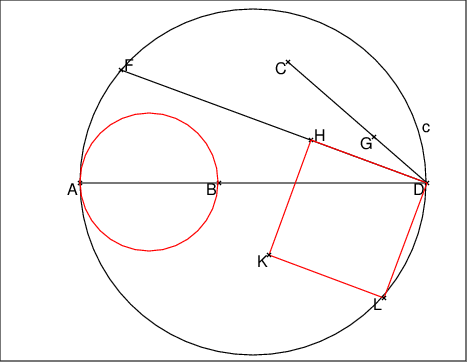
\includegraphics[width=\textwidth]{picarre}\\
On a :\\
{\tt normal(longueur(A,C));} renvoie {\tt 2*sqrt(3)}\\
{\tt normal(longueur2(F,D)} renvoie {\tt 22}\\
{\tt normal(longueur2(D,C));} renvoie {\tt 7}\\
{\tt normal(longueur2(D,G))} renvoie {\tt 1}\\
{\tt normal(longueur(H,D));} renvoie {\tt (sqrt(154))/7}\\
{\tt normal(longueur2(H,D));} renvoie {\tt 22/7}\\
{\tt aire(carre(D,H))} renvoie {\tt 22/7}
\section{Construction par Ramanujan d'un carr\'e d'aire $\frac{355}{113}$}
En 1913 Ramanujan proposa la construction d'un carr\'e ayant pour aire celle
d'un cercle de rayon 1 avec une erreur de $1.47*10^{-5}$.\\
Ce carr\'e a pour cot\'e : $\frac{\sqrt{355}}{\sqrt 113}$.\\
On a :\\
$355=18^2+31$ et $113=12^2-31$\\
$\frac{355}{9^2}=4+\frac{31}{9^2}$ et $\frac{113}{6^2}=4-\frac{31}{6^2}$\\
Il reste a construire $\sqrt{31}$.\\
On a :\\
$31=6^2-5$\\
Voici la construction de ce carr\'e faite par Ramanujan.\\
Soit le cercle $c$ de centre $O$ et de diam\`etre $PR=2$.\\
Avec {\tt Xcas}, on prend :\\
{\tt O:=point(0);P:=point(-1);R:=point(1);}\\
{\tt H:=point(-1/2);T:=point(2/3);}\\
Le cercle $c$ passe par le point {\tt Q:=point(2/3+i*sqrt(5)/3);}\\
On a {\tt RS=QT=sqrt(5)/3}\\
On d\'efinit les projections $M$ et $N$ respectives  $M$ et $N$ de $O$ et $T$
sur $PS$.\\
On d\'efinit :\\
{\tt L:=point(-1-i*longueur(M,N));}\\
{\tt K} sur le cercle $c$ tel que $PK=PM$\\
{\tt C} sur le segment $RK$ tel que $RC=RH=3/2$
{\tt D} sur le segment $RL$ tel que $CD//KL$\\
Le carr\'e de c\^ot\'e $RD$ a alors pour c\^ot\'e :\\
$$\sqrt{\frac{355}{113}}$$
Avec {\tt Xcas}, ontape :
\begin{verbatim}
O:=point(0);
P:=point(-1);
R:=point(1);
H:=point(-1/2);
T:=point(2/3);
c:=cercle(O,1,affichage=4+epaisseur_ligne_2);
Q:=point(2/3+i*sqrt(5)/3);
S:=inter_unique(c,cercle(R,sqrt(5)/3),Q);
s:=segment(P,S);
M:=projection(s,O);
N:=projection(s,T);
L:=point(-1-i*longueur(M,N));
K:=inter_unique(c,cercle(P,longueur(P,M)),L);
C:=inter_unique(droite(R,K),cercle(R,3/2),K);
D:=inter_unique(droite(L,R),parallele(C,droite(L,K)));
carre(D,R,affichage=1+epaisseur_ligne_2);
segment(P,L);
segment(R,S);
segment(R,L);
segment(R,K);
segment(L,K);
segment(D,C);
segment(O,M);
segment(T,N);
cercle(P,longueur(M,P),affichage=ligne_tiret_point);
cercle(R,3/2,affichage=ligne_tiret_point);
\end{verbatim}
On tape :\\
{\tt evalf(aire(carre(D,R)))}\\
On obtient :\\
{\tt 3.14157798199}\\
On tape :\\
{\tt evalf(pi-aire(carre(D,R)))}\\
On obtient :\\
{\tt 1.46716034237e-05}\\

On obtient la figure :\\
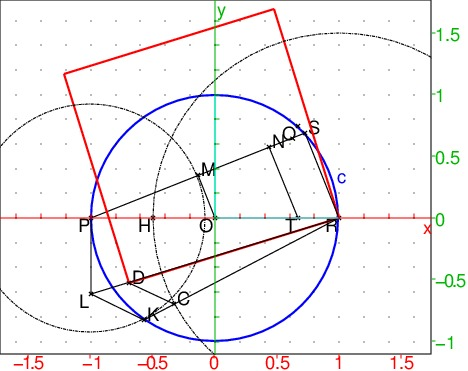
\includegraphics[width=\textwidth]{picarre2}

{\bf Calcul de $RD^2$}\\
On a :\\
$RS^2=5/9$\\
$PS^2=4-5/9=31/9$\\
$PK^2=PM^2=PS^2/4=31/36$\\
$PL^2=MN^2=PS^2/9=31/81$\\
$RK^2=4-PK^2=113/36$\\
$RL^2=4+PL^2=355/81$\\
$RC^2=RH^2=9/4$\\
$\frac{RD^2}{RL^2}=\frac{R^2C}{RK^2}=\frac{81}{113}$\\
Donc $RD^2=\frac{355}{113}$

\section{Une valeur approch\'ee de $\pi$ par $(9^2+19^2/22)^(1/4)$}
\noindent On tape :\\
{\tt A:=(9\verb|^|2+19\verb|^|2/22)\verb|^|(1/4)}\\
{\tt evalf(A)}\\
On obtient :\\
{\tt 3.14159265258}\\
On tape :
{\tt evalf(pi)}\\
On obtient :
{\tt 3.14159265359}\\
On tape :\\
{\tt evalf(pi-A)}\\
On obtient :\\
{\tt 1.00715169538e-09}


\section{Un nombre quasi-entier : $(\frac{\ln(5280^3*(236674+30303*\sqrt{61})^3+744)}{\pi})^2$}
\noindent Avec {\tt Xcas}, on tape :\\
{\tt A:=ln(5280\verb|^|3*((236674+30303*sqrt(61))\verb|^|(3))+744)}\\
{\tt evalf((A/pi)\verb|^|2)}\\
On obtient :\\
{\tt 427.0}\\
On tape :\\
{\tt evalf((A/pi)\verb|^|2,52)}\\
On obtient :\\
{\tt 0.4270000000000000000000000000000000000000000000000000e3}\\
On tape :\\
{\tt evalf((A/pi)\verb|^|2,55)}\\
On obtient :\\
{\tt 0.4270000000000000000000000000000000000000000000000000106e3}\\

\chapter{Pour trouver les premi\`eres d\'ecimales de $\pi$}
\section{La formule de Gregory et le d\'eveloppement en s\'erie de $\arctan(x)$}
La s\'erie de Gregory est le d\'eveloppement en s\'erie enti\`ere de $\arctan(x)$\\
On a :
$$\arctan(x)=x-\frac{x^3}{3}+\frac{x^5}{5}+...+(-1)^k\frac{x^{2k+1}}{2k+1}+...$$
Le reste de cette s\'erie altern\'ee est du signe du premier terme n\'eglig\'e
et est major\'e en valeur absolue par la valeur absolue du premier terme n\'eglig\'e.
\section{La formule de Machin}
De la formule d'addition des tangentes \`a savoir :
$$\tan(a+b)=\frac{\tan(a)+\tan(b)}{1-\tan(a)*\tan(b)}$$
on en d\'eduit la formule pour $ab<1$ :
$$\arctan(a)+\arctan(b)=\arctan(\frac{a+b}{1-ab})$$

Exercices :\\
1/ Pour $a=1/5$ on cherche $b$ pour que :
$$\arctan(a)+\arctan(b)=\arctan(1)=\frac{\pi}{4}$$
On doit donc r\'esoudre :
$$\frac{a+b}{1-ab}=1$$
On trouve :
$$b=\frac{1-a}{1+a}=\frac{2}{3}$$
Donc :
$$\arctan(\frac{1}{5})+\arctan(\frac{2}{3})=\frac{\pi}{4}$$
2/  Pour $a=1/5$ on cherche $b$ pour que :
$$\arctan(a)+\arctan(b)=\arctan(\frac{2}{3})$$
On doit donc r\'esoudre :
$$\frac{a+b}{1-ab}=c=\frac{2}{3}$$
On trouve :
$$b=\frac{c-a}{1+ac}=\frac{\frac{2}{3}-\frac{1}{5}}{1\frac{2}{15}}=\frac{7}{17}$$
Donc :
$$2\arctan(\frac{1}{5})+\arctan(\frac{7}{17})=\frac{\pi}{4}$$
3/ En faisant encore deux fois le m\^eme genre de substitution, montrer la 
formule de Machin  :
$$4\arctan(\frac{1}{5})-\arctan(\frac{1}{239})=\frac{\pi}{4}$$
Pour cela on prend successivement :\\
$c=\frac{7}{17}$ et on trouve $b=\frac{c-a}{1+ac}=\frac{9}{46}$ et\\
$c=\frac{9}{46}$ et on trouve $b=\frac{c-a}{1+ac}=\frac{-1}{239}$\\
4/ \'Ecrire un programme qui prend en entr\'ee $a$ et $n$ et qui
renvoie la liste $L$ des valeurs de $b_k$ v\'erifiant :\\
$k\arctan(a)+\arctan(b_k)=\frac{\pi}{4}$ pour $k=1..n$ ($L[k-1]=b_k$)\\
On tape le programme :
\begin{verbatim}
machin1(a,n):={
local k,c,L;
c:=1;
L:=[0];
for (k:=1;k<n+1;k:=k+1) {
c:=(c-a)/(1+a*c);
L:=append(L,c);
}
return(L);
};
\end{verbatim}
On tape :\\
{\tt machin1(1/5,5)}\\
On obtient :\\
{\tt [0,2/3,7/17,9/46,1/-239,-122/597]}\\
Ainsi, pour  $a=1/5$ et $k=3$, $b_k=9/46$ donc :\\
${\tt 3\arctan(\frac{1}{5})+\arctan(\frac{9}{46})=\frac{\pi}{4}}$\\ 
On tape :\\
{\tt machin1(1/3,5)}\\
On obtient :\\
{\tt [0,1/2,1/7,-2/11,-17/31,-41/38]}\\
Ainsi, pour $a=1/3$ et $k=2$, $b_k=1/7$ donc :\\
${\tt 2\arctan(\frac{1}{3})+\arctan(\frac{1}{7})=\frac{\pi}{4}}$\\ 
\section{Les d\'ecimales de $\pi$ avec les formules pr\'ec\'edentes}
\subsection{Une remarque}
Si on utilise pour calculer $\pi$ la formule :\\
$$\arctan(x)=x-\frac{x^3}{3}+\frac{x^5}{5}+...+(-1)^k\frac{x^{2k+1}}{2k+1}+...$$\\
Si on prend  $x=1$, on a $\arctan(1)=\pi/4=1-\frac{1}{3}+\frac{1}{5}+...+(-1)^k\frac{1}{2k+1}+...$ mais la convergence est lente.\\
On remarque que la convergence  est beaucoup plus rapide pour $x=1/5$
et encore plus rapide pour $x=1/239$ d'o\`u l'utilisation de la formule :\\
$$\frac{\pi}{4}=4\arctan(\frac{1}{5})-\arctan(\frac{1}{239})$$
\subsection{Le programme avec {\tt Xcas}}
Pour calculer la somme de $n$ termes de la s\'erie on va utiliser la m\'ethode 
de H\"orner pour faire le moins possibles de multiplications, on a :\\
$\arctan(x)=x(1-x^2(\frac{1}{3}-x^2(\frac{1}{5}-x^2(....-x^2(\frac{1}{2n-1})))))$ \\
L'utilisateur doit rentrer la valeur de $x$ ($a$) et le nombre $n$ de termes de 
la s\'erie. 
\begin{verbatim}
//approx de arctan(a) par sa serie :
// a-a^3/3+..+(-1)^n*a^(2n+1)/(2n+1) 
//cette valeur est calculee par la methode de Horner
gregory(a,n):={
local t,k;
t:=1/(2*n-1);
for (k:=2*n-3;k>0;k:=k-2) {
t:=1/k-a^2*t;
}
return (a*t);
};
\end{verbatim}
On tape :\\
{\tt 16*gregory(1/5,18)-4*gregory(1/239,6)}\\
On obtient :\\
{\tt 3.14159265359}
On tape :\\
{\tt evalf(16*gregory(1/5,42)-4*gregory(1/239,20))}\\
On obtient, si on a choisit 60 {\tt Chiffres} dans la configuration du CAS (menu
{\tt Cfg->Configuration du CAS}) :\\
{\tt 3.14159265358979323846264338327950288419716939937510582097494}
\subsection{Combien faut-il calculer de termes ?}
Soit $R_n(x)$ le reste de la s\'erie $\sum_{k=1}^\infty (-1)^{k+1}\frac{x^{2k-1}}{2k-1}$ : $R_n(x)=\sum_{k=n+1}^\infty (-1)^{k+1}\frac{x^{2k-1}}{2k-1}$.\\
On sait que $|R_n(x)|<\frac{|x|^{2n+1}}{2n+1}$
Pour avoir $|R_n(1/5)|=|R_n(0.2)|<10^{-61}$ il faut que :\\
$2^{2n+1}<(2n+1)10^{2n-60}$ et comme $2^10\simeq 10^3$ cela donne si on 
suppose $2n+1>10$ :\\
$10^{(6n+3)/10}<10^{2n-59}$ soit $593<14n$ soit $n\simeq 42$
On v\'erifie pour $n=42$ on a $\frac{(1/5)^{85}}{85}<2.56e-62$\\
On peut aussi \'ecrire si on suppose que $2n+1>10$ :\\
$\frac{|x|^{2n+1}}{2n+1}<x^{2n+1}/10<10^{-61}$
donc on va choisir $x^{2n+1}<10^{-60}$ soit $(2n+1)log10(x)<-60$
ou encore $n>((-60)/log10(x)-1)/2$
Pour $x=1/5$ on a $n>42.4202967422$ et comme $2n+1>40$ on peut am\'eliorer la 
majoration $\frac{|x|^{2n+1}}{2n+1}<x^{2n+1}/40<10^{-61}$\\
ce qui donne $n>((-60+log10(4))/log10(1/5)-1)/2=41.9896201841$ donc on prend 
$n=42$\\
pour $x=1/293$ on a $n>11.66$ donc on prend $n=12$ et on
v\'erifie : $\frac{(1/239)^{25}}{25}=1.38711499837e-61$.\\
On choisit 62 {\tt Chiffres}  dans la configuration du CAS (menu
{\tt Cfg->Configuration du CAS}) et on tape :\\
{\tt evalf(16*gregory(1/5,42)-4*gregory(1/239,12))}\\
On obtient :\\
{\tt 3.1415926535897932384626433832795028841971693993751058209749446}\\
On tape :\\
{\tt evalf(pi)}\\
On obtient :\\
{\tt 3.1415926535897932384626433832795028841971693993751058209749446}\\
{\bf Remarque}\\
Avec cette m\'ethode John Machin calcula 100 d\'ecimales de $\pi$ en 1706.
\subsection{Les formules de m\^eme type que celles de Machin}
En 1973, Jean Guilloud a mis une journ\'ee pour calculer $10^6$ d\'ecimales de $\pi$ en utilisant une formule de m\^eme type \`a savoir :
$$6\arctan(\frac{1}{8})+2\arctan(\frac{1}{57})+\arctan(\frac{1}{239})=\frac{\pi}{4}$$
en v\'erifiant ses calculs avec la formule analogue :
$$12\arctan(\frac{1}{18})+8\arctan(\frac{1}{57})-5\arctan(\frac{1}{239})=\frac{\pi}{4}$$
En 1999, Yasumata Kanadaa a atteint le record en calculant $12411* 10^8$ d\'ecimales de $\pi$ en utilisant une formule de m\^eme type \`a savoir :
$$24\arctan(\frac{1}{12943})-12\arctan(\frac{1}{682}) +44\arctan(\frac{1}{57})+7\arctan(\frac{1}{239})=\frac{\pi}{4}$$
et la formule analogue :
$$12\arctan(\frac{1}{49})+32\arctan(\frac{1}{57})-5\arctan(\frac{1}{239})+12\arctan(\frac{1}{110443})=\frac{\pi}{4}$$
On peut v\'erifier ces formules avec {\tt Xcas}, on tape par exemple :\\
{\tt tsimplify(12*atan(1/49)+32*atan(1/57)-5*atan(1/239)+12*atan(1/110443))}
On obtient :\\
${\tt \frac{\pi}{4}}$\\
{\bf Comment trouver des formules de type Machin ?}\\
voir aussi \ref{sec:Todd}\\
Montrons pour cela que si $a \in \N^*$ et si $a^2+1=a_1*a_2$  avec 
$(a_1,a_2) \in \Z^2$ et $(a+a_1)(a+a-2)\neg 0$  alors on a :\\
$\arctan(1/a)=\arctan(1/(a+a_1))+\arctan(1/(a+a_2))$ (si $a\geq 2$ alors $a$ ne
divise pas $a^2+1$ donc $a+a-1$ et $a+a_2$ sont non nuls et diff\'erents).\\
On a si $xy<1$, $\arctan(x)+\arctan(y)=\arctan((x+y)/(1-xy))$ donc\\
$\arctan(1/(a+a_1))+\arctan(1/(a+a_2))=\arctan((2a+a_1+a_2)/((a+a_1)(a+a_2)-1))=\arctan(1/a)$ puisque 
\begin{itemize}
\item si $a+a_1>1$ et $a+a_2>1$ alors $1/(a+a_1)*1/(a+a_2)<1$ 
\item si $a+a_1>1$ et $a+a_2<-1$ alors $1/(a+a_1)*1/(a+a_2)<0<1$ 
\item si $a+a_1\leq -1$ et $a+a_2<-1$ alors $1/(a+a_1)*1/(a+a_2)=1/(-a-a_1)*1/(-a-a_2)<1$ 
\end{itemize}
Donc :\\
si $a^2+1=a_1*a_2$ alors  $\arctan(1/(a+a_1))+\arctan(1/(a+a_2))=\arctan(1/a)$\\
{\bf Exemples}\\
si $a=1$ on a $\arctan(1)=\arctan(1/2)+\arctan(1/3)$.\\
si $a=2$ on a $\arctan(1/2)=\arctan(1/3)+\arctan(1/7)$ et\\
$\arctan(1/2)=\arctan(1/(2-1))+\arctan(1/(2-5))=\arctan(1)-\arctan(1/3)$
On a donc :\\
$a=1$ $a^2+1=2=1*2$ donc $\pi/4=\arctan(1)=\arctan(1/2)+\arctan(1/3)$\\
$a=2$ $a^2+1=5=1*5$ donc $\arctan(1/2)=\arctan(1/3)+\arctan(1/7)$ et\\
$\arctan(1/2)=\arctan(1/(2-1))+\arctan(1/(5-2))=\arctan(1)-\arctan(1/3)$
$a=3$ $a^2+1=10=1*10=2*5$ donc $\arctan(1/3)=\arctan(1/4)+\arctan(1/13)=\arctan(1/5)+\arctan(1/8)$ et
$\arctan(1/3)=\arctan(1/(3-2))+\arctan(1/(3-5))=\arctan(1)-\arctan(1/2)$\\
$a=5$ $a^2+1=26=1*26=2*13$ donc $\arctan(1/5)=\arctan(1/7)+\arctan(1/18)=\arctan(1/6)+\arctan(1/31)$ et\\
$\arctan(1/5)=\arctan(1/(5-2))+\arctan(1/(5-13))=\arctan(1/3)-\arctan(1/8)$
$a=7$ $a^2+1=50=1*50=2*25$ donc $\arctan(1/7)=\arctan(1/8)+\arctan(1/57)=\arctan(1/9)+\arctan(1/32)$ et \\
$\arctan(1/7)=\arctan(1/(7-2))+\arctan(1/(7-25))=\arctan(1/5)-\arctan(1/18)$\\

On en d\'eduit donc que :
$$\pi/4=2\arctan(1/3)+\arctan(1/7)$$
$$\pi/4=2\arctan(1/3)+\arctan(1/5)-\arctan(1/18)$$
$$\pi/4=2\arctan(1/3)+\arctan(1/5)-\arctan(1/18)$$
$$\pi/4=2\arctan(1/3)+\arctan(1/8)+\arctan(1/57)$$
$$\pi/4=3\arctan(1/3)-\arctan(1/5)+\arctan(1/57)$$
et en utilisant $\pi/4=4\arctan(1/5)-\arctan(1/239)$  on retrouve facilement 
les 2 formules utilis\'ees par Jean Guilloud :\\
$6\arctan(\frac{1}{8})+(6-4)\arctan(\frac{1}{57})+\arctan(\frac{1}{239})=$\\
$6(\pi/4-2\arctan(1/3))-4(\pi/4-3\arctan(1/3)+\arctan(1/5))-\pi/4+4\arctan(1/5)=$\\
$\pi/4$ \\
et\\
$12\arctan(\frac{1}{18})+8\arctan(\frac{1}{57})-5\arctan(\frac{1}{239})=$\\
$12(-\pi/4+2\arctan(1/3)+\arctan(1/5))+8(\pi/4-3\arctan(1/3)+\arctan(1/5))+5(\pi/4-4\arctan(1/5))=\pi/4$
\section{Pour bien afficher les d\'ecimales}
\begin{verbatim}
//approx de arctan(a) par a-a^3/3+..+(-1)^n*a^(2n+1)/(2n+1) 
//valeur de la serie est calculee par la methode de Horner
gregory(a,n):={
local t,k;
t:=1/(2*n-1);
for (k:=2*n-3;k>0;k:=k-2) {
t:=1/k-a^2*t;
}
return (a*t);
}
:;
//pour afficher selon un tableau
affiche1(fl,n):={
local s,p,q,j,k,L,LT;
L:="";
s:=string(fl);
p:=size(s);
q:=iquo(p,11*n)
si irem(p,11*n)==0 alors 
LT:=[0$q];sinon 
LT:=[0$(q+1)];
fsi;
pour j de 0 jusque q-1 faire
pour k de 1 jusque 11 faire
L:=L+mid(s,0,n)+" ";
s:=mid(s,n);
fpour;
LT[j]=<[L];
L:="";
fpour;
si r!=0 alors
pour k de 1 jusque size(s) faire
L:=L+mid(s,0,n)+" ";
s:=mid(s,n);
fpour;
LT[q]=<[L];
fsi;
return LT;
}:;
//pour afficher selon une liste de chaines
affiche2(fl,n):={
local s,p,q,j,k,L,LT;
L:="";
s:=string(fl);
p:=size(s);
q:=iquo(p,11*n);
r:=irem(p,11*n);
si r==0 alors 
LT:=[0$q];sinon 
LT:=[0$q+1];
fsi;
pour j de 0 jusque q-1 faire
pour k de 1 jusque 11 faire
L:=L+mid(s,0,n)+" ";
s:=mid(s,n);
fpour;
LT[j]=<L;
L:="";
fpour;
si r!=0 alors
pour k de 1 jusque size(s) faire
L:=L+mid(s,0,n)+" ";
s:=mid(s,n);
fpour;
LT[q]=<L;
fsi;
return LT;
}:;
\end{verbatim}
On v\'erifie pour $n=2900$ on a $\frac{(1/5)^{85}}{5801}<0.33e-4058$\\
et on v\'erifie pour $n=860$ on a  $\frac{(1/239)^{11721}}{1721}=0.35e-4096$.\\
On tape :\\
{\tt (1/5.)\verb|^|5801/5801,(1/239.)\verb|^|1721/1721}\\
On obtient :\\
{\tt 0.3247147235398264366269e-4058,0.347881711410409416161e-4096}\\
{\tt Digits:=4000}\\
On tape :\\
{\tt LR1:=affiche1(evalf(16*gregory(1/5,2900)-4*gregory(1/239,860)),5)}\\
On obtient  comme r\'eponse une matrice.\\
Ou on tape :\\
{\tt LR2:=affiche2(evalf(16*gregory(1/5,2900)-4*gregory(1/239,860)),5)}\\
{\tt pour j de 0 jusque size(LR2)-1 faire print(LR2[j]) fpour}
On obtient apr\`es 0.88s:\\
\begin{verbatim}
3.141 59265 35897 93238 46264 33832 79502 88419 71693 99375 10582 
09749 44592 30781 64062 86208 99862 80348 25342 11706 79821 48086 
51328 23066 47093 84460 95505 82231 72535 94081 28481 11745 02841 
02701 93852 11055 59644 62294 89549 30381 96442 88109 75665 93344 
61284 75648 23378 67831 65271 20190 91456 48566 92346 03486 10454 
32664 82133 93607 26024 91412 73724 58700 66063 15588 17488 15209 
20962 82925 40917 15364 36789 25903 60011 33053 05488 20466 52138 
41469 51941 51160 94330 57270 36575 95919 53092 18611 73819 32611 
79310 51185 48074 46237 99627 49567 35188 57527 24891 22793 81830 
11949 12983 36733 62440 65664 30860 21394 94639 52247 37190 70217 
98609 43702 77053 92171 76293 17675 23846 74818 46766 94051 32000 
56812 71452 63560 82778 57713 42757 78960 91736 37178 72146 84409 
01224 95343 01465 49585 37105 07922 79689 25892 35420 19956 11212 
90219 60864 03441 81598 13629 77477 13099 60518 70721 13499 99998 
37297 80499 51059 73173 28160 96318 59502 44594 55346 90830 26425 
22308 25334 46850 35261 93118 81710 10003 13783 87528 86587 53320 
83814 20617 17766 91473 03598 25349 04287 55468 73115 95628 63882 
35378 75937 51957 78185 77805 32171 22680 66130 01927 87661 11959 
09216 42019 89380 95257 20106 54858 63278 86593 61533 81827 96823 
03019 52035 30185 29689 95773 62259 94138 91249 72177 52834 79131 
51557 48572 42454 15069 59508 29533 11686 17278 55889 07509 83817 
54637 46493 93192 55060 40092 77016 71139 00984 88240 12858 36160 
35637 07660 10471 01819 42955 59619 89467 67837 44944 82553 79774 
72684 71040 47534 64620 80466 84259 06949 12933 13677 02898 91521 
04752 16205 69660 24058 03815 01935 11253 38243 00355 87640 24749 
64732 63914 19927 26042 69922 79678 23547 81636 00934 17216 41219 
92458 63150 30286 18297 45557 06749 83850 54945 88586 92699 56909 
27210 79750 93029 55321 16534 49872 02755 96023 64806 65499 11988 
18347 97753 56636 98074 26542 52786 25518 18417 57467 28909 77772 
79380 00816 47060 01614 52491 92173 21721 47723 50141 44197 35685 
48161 36115 73525 52133 47574 18494 68438 52332 39073 94143 33454 
77624 16862 51898 35694 85562 09921 92221 84272 55025 42568 87671 
79049 46016 53466 80498 86272 32791 78608 57843 83827 96797 66814 
54100 95388 37863 60950 68006 42251 25205 11739 29848 96084 12848 
86269 45604 24196 52850 22210 66118 63067 44278 62203 91949 45047 
12371 37869 60956 36437 19172 87467 76465 75739 62413 89086 58326 
45995 81339 04780 27590 09946 57640 78951 26946 83983 52595 70982 
58226 20522 48940 77267 19478 26848 26014 76990 90264 01363 94437 
45530 50682 03496 25245 17493 99651 43142 98091 90659 25093 72216 
96461 51570 98583 87410 59788 59597 72975 49893 01617 53928 46813 
82686 83868 94277 41559 91855 92524 59539 59431 04997 25246 80845 
98727 36446 95848 65383 67362 22626 09912 46080 51243 88439 04512 
44136 54976 27807 97715 69143 59977 00129 61608 94416 94868 55584 
84063 53422 07222 58284 88648 15845 60285 06016 84273 94522 67467 
67889 52521 38522 54995 46667 27823 98645 65961 16354 88623 05774 
56498 03559 36345 68174 32411 25150 76069 47945 10965 96094 02522 
88797 10893 14566 91368 67228 74894 05601 01503 30861 79286 80920 
87476 09178 24938 58900 97149 09675 98526 13655 49781 89312 97848 
21682 99894 87226 58804 85756 40142 70477 55513 23796 41451 52374 
62343 64542 85844 47952 65867 82105 11413 54735 73952 31134 27166 
10213 59695 36231 44295 24849 37187 11014 57654 03590 27993 44037 
42007 31057 85390 62198 38744 78084 78489 68332 14457 13868 75194 
35064 30218 45319 10484 81005 37061 46806 74919 27819 11979 39952 
06141 96634 28754 44064 37451 23718 19217 99983 91015 91956 18146 
75142 69123 97489 40907 18649 42319 61567 94520 80951 46550 22523 
16038 81930 14209 37621 37855 95663 89377 87083 03906 97920 77346 
72218 25625 99661 50142 15030 68038 44773 45492 02605 41466 59252 
01497 44285 07325 18666 00213 24340 88190 71048 63317 34649 65145 
39057 96268 56100 55081 06658 79699 81635 74736 38405 25714 59102 
89706 41401 10971 20628 04390 39759 51567 71577 00420 33786 99360 
07230 55876 31763 59421 87312 51471 20532 92819 18261 86125 86732 
15791 98414 84882 91644 70609 57527 06957 22091 75671 16722 91098 
16909 15280 17350 67127 48583 22287 18352 09353 96572 51210 83579 
15136 98820 91444 21006 75103 34671 10314 12671 11369 90865 85163 
98315 01970 16515 11685 17143 76576 18351 55650 88490 99898 59982 
38734 55283 31635 50764 79185 35893 22618 54896 32132 93308 98570 
64204 67525 90709 15481 41654 98594 61637 18027 09819 94309 92448 
89575 71282 89059 23233 26097 29971 20844 33573 26548 93823 91193 
25974 63667 30583 60414 28138 83032 03824 90375 89852 43744 17029 
13276 56180 93773 44403 07074 69211 20191 30203 30380 19762 11011 
00449 29321 51608 42444 85963 76698 38952 28684 78312 35526 58213 
14495 76857 26243 34418 93039 68642 62434 10773 22697 80280 73189 
15441 10104 46823 25271 62010 52652 27211 
\end{verbatim}
\section{La formule de Bailey-Borwein-Plouffe (BBP)}
\subsection{L'historique}
En 1995, Plouffe (avec Bailey et Borwein) a d\'ecouvert la formule de 
Bailey-Borwein-Plouffe (BBP) qui permet de calculer le $n$-ième bit de $\pi$ 
sans avoir à calculer d'autres bits. Un an
plus tard, il publie un nouvel article sur la formule, permettant de 
d\'eterminer le $n$-ième chiffre en base 10 de $\pi$, mais le temps de calcul, 
bien que relativement court, n'est pas lin\'eaire.

Il est \'egalement le co-auteur de l'Encyclop\'edie en ligne des suites de 
nombres entiers.

L'Inverseur de Plouffe est une page web qui contient plus de 200 millions de 
constantes math\'ematiques. Un r\'epertoire est accessible et contient plus de 
3,93 milliards de constantes \`a une pr\'ecision de 64 chiffres d\'ecimaux au 
21 juillet 2009.

Pour l'anecdote, Simon Plouffe a d\'etenu en 1977 le record Guinness de 
m\'emorisation des d\'ecimales de $\pi$, avec 4 096 d\'ecimales. Il en avait 
m\'emoris\'e 4 400, mais en a r\'ecit\'e seulement 4 096 parce que 
$4096=2^{12}$).

La formule de Plouffe ou formule BBP est 
$$\pi=\sum_{n=0}^{+\infty}\frac{1}{16^k}(\frac{4}{8k+1}-\frac{2}{8k+4}-\frac{1}{8k+5}-\frac{1}{8k+6})$$

\subsection{D\'emonstration de la formule de Plouffe en devoir (Universit\'e de Lorraine)}
Le but de cet exercice est de montrer la formule de Plouffe
$$\pi=\sum_{k=0}^{+\infty}\frac{1}{16^k}(\frac{4}{8k+1}-\frac{2}{8k+4}-\frac{1}{8k+5}-\frac{1}{8k+6})$$
%47/15+106/819+829/19635+316/15225=3.14159245757
\begin{enumerate}
\item Montrer que pour tout $a$ r\`eel avec $0 < a < 1$, pour tous $n, p \geq 1$
on a
$$\int_0^a\frac{x^{n-1}}{1-x^p}=\sum_{k=0}^{+\infty}\frac{a^{kp+n}}{kp+n}$$
\item En d\'eduire que
$$\sum_{k=0}^{+\infty}\frac{1}{16^k}(\frac{4}{8k+1}-\frac{2}{8k+4}-\frac{1}{8k+5}-\frac{1}{8k+6})=16\int_0^1\frac{4-2x^3-x^4-x^5}{16-x^8}dx$$
\item Simplifier la fraction $\displaystyle \frac{4-2x^3-x^4-x^5}{16-x^8}$ (on
pourra remarquer que le polyn\^ome $4-2x^3-x^4-x^5$ a une racine simple), puis
d\'ecomposer la fraction obtenue en \'el\'ements simples dans $\Q[X]$.
\item Conclure
\end{enumerate}
{\bf Solution avec l'aide de {\tt Xcas}}
On utilise ici {\tt Xcas} en mode r\'eel pour
v\'erifier ou pour faire des calculs.
\begin{enumerate}
\item Pour $|x| < 1$ et $p>1$, on a  $|x^p | < 1$. On a donc le d\'eveloppement
 en s\'erie enti\`ere :
$$\frac{x^{n-1}}{1-x^p}=x^{n-1}\sum_{k=0}^{+\infty}x^{kp}=\sum_{k=0}^{+\infty}x^{kp+n-1}$$
Avec {\tt Xcas}, on v\'erifie et on tape :\\
{\tt assume(p,integer);sum(x\verb|^|(k*p),k=0..inf)}\\
On obtient : {\tt x\verb|^|(-p)/(x\verb|^|(-p)-1)}\\
A l’int\'erieur du rayon de convergence, on peut int\'egrer terme \`a terme et
comme $\int_0^ax^{kp+n-1}dx=\frac{a^{kp+n}}{kp+n}$, on obtient :
$$\int_0^a\frac{x^{n-1}}{1-x^p}dx=\sum_{k=0}^{+\infty}\frac{a^{kp+n}}{kp+n}$$
Avec {\tt Xcas}, on v\'erifie et on tape :\\
{\tt int(x\verb|^|(k*p+n-1),x=0..a)}\\
On obtient : {\tt a\verb|^|(k*p+n)/(k*p+n)}

\item Remarquons tout d'abord que :\\
$\displaystyle\int_0^1\frac{x^m}{16-x^8}dx=\int_0^1\frac{x^m}{16(1-{(\frac{x}{\sqrt 2})}^8}dx=
\int_0^{\frac{\sqrt 2}{2}}\frac{1}{16}\frac{u^m*{\sqrt 2}^{m+1}}{1-u^8}du$\\
Avec {\tt Xcas}, on tape pour faire  le changement de variable $x=u\sqrt 2$
dans l'int\'egrale :\\
{\tt subst('int(x\verb|^|m/(16-x\verb|^|8),x,0,1)',x=sqrt(2)*u)}\\
On obtient :\\
{\tt int((sqrt(2)*u)\verb|^|m*1/(16-(sqrt(2)*u)\verb|^|8)*sqrt(2),}\\
\hspace*{3cm}{\tt u,0,(sqrt(2))/2)}\\
Puis, on s\'electionne {
\tt sqrt(2)*u)\verb|^|m*1/(16-(sqrt(2)*u)\verb|^|8)*sqrt(2)}, on
appelle {\tt simplify} et on obtient :\\
{\tt int(-(sqrt(2)*u)\verb|^|m*sqrt(2)/(16*u\verb|^|8-16), u,0,(sqrt(2))/2)}\\
D'apr\'es ce qui pr\'ec\'ede (pour $p=8$, $m=n-1$ et $a=\frac{\sqrt 2}{2}$)
et puisque :\\
$\displaystyle{\sqrt 2}^{m+1}*a^{8k+m+1}=\frac{1}{{\sqrt 2}^{8*k}}=\frac{1}{16^*k}$, on a :\\
$$\int_0^1\frac{x^m}{16-x^8}dx=\frac{1}{16}\sum_{k=0}^{+\infty}\frac{1}{16^k*(8k+m+1)}=\frac{1}{16}\sum_{k=0}^{+\infty}\frac{1}{16^k*(8k+m+1)}$$
Donc :\\
$$16\int_0^1\frac{4-2x^3-x^4-x^5}{16-x^8}dx=
\sum_{k=0}^{+\infty}\frac{1}{16^k}(\frac{4}{8k+1}-\frac{2}{8k+4}-\frac{2}{8k+5}- \frac{1}{8k+6})$$

\item {\bf Factorisation de $4-2x^3-x^4-x^5$}\\
1 est racine \'evidente de $4-2x^3-x^4-x^5$.\\
On tape :\\
{\tt factor(4-2x\verb|^|3-x\verb|^|4-x\verb|^|5)}\\
On obtient :\\
{\tt -(x-1)*(x\verb|^|2+2)*(x\verb|^|2+2*x+2)}\\
On a donc la factorisation
$$x^5 + x^4 + 2x^3 -4 = (x-1)(x^2 + 2)(x^2 + 2x + 2)$$
{\bf Factorisation de $16-x^8$}\\
On tape :\\
{\tt factor(16-x\verb|^|8)}\\
On obtient :\\
{\tt -(x\verb|^|2-2)*(x\verb|^|2+2)*(x\verb|^|2-2*x+2)*(x\verb|^|2+2*x+2)}\\
{\bf Simplification de $\displaystyle\frac{4-2x^3-x^4-x^5}{16-x^8}$}\\
On tape :\\
{\tt normal((4-2x\verb|^|3-x\verb|^|4-x\verb|^|5)/(16-x\verb|^|8))}\\
On obtient :\\
{\tt (x-1)/(x\verb|^|4-2*x\verb|^|3+4*x-4)}\\
{\bf D\'ecomposition en \'el\'ements simples de $\displaystyle\frac{4-2x^3-x^4-x^5}{16-x^8}$}\\
On tape :\\
{\tt  partfrac((x-1)/(x\verb|^|4-2*x\verb|^|3+4*x-4))}\\
On obtient :\\
{\tt x/((x\verb|^|2-2)*4)+(-x+2)/((x\verb|^|2-2*x+2)*4)}\\
Ou bien , on tape directement :\\
{\tt partfrac((4-2x\verb|^|3-x\verb|^|4-x\verb|^|5)/(16-x\verb|^|8))}\\
On obtient :\\
{\tt x/((x\verb|^|2-2)*4)+(-x+2)/((x\verb|^|2-2*x+2)*4)}
\item {\bf Conclusion}\\
On a donc :\\
$\displaystyle 16\int_0^1\frac{4-2x^3-x^4-x^5}{16-x^8}dx=4\int_0^1\frac{x}{x^2-2}dx+4\int_0^1\frac{-x+2}{x^2-2*x+2}dx=$\\
$\displaystyle 2\ln(|1^2-2|)-2\ln(|0^2-2|)-2\int_0^1\frac{2x-2}{x^2-2*x+2}dx+4\int_0^1\frac{1}{x-1)^2+1}dx=-2\ln(2)+2\ln(2)+4*\atan(0)-4*\atan(-1)=\pi$\\
On tape :\\
{\tt normal(16*int((4-2x\verb|^|3-x\verb|^|4-x\verb|^|5)/(16-x\verb|^|8),x=0..1))}\\
On obtient :\\
{\tt pi}\\
Donc :
$$\pi=\sum_{n=0}^{+\infty}\frac{1}{16^k}(\frac{4}{8k+1}-\frac{2}{8k+4}-\frac{1}{8k+5}-\frac{1}{8k+6})$$
Avec {\tt Xcas}, en mode r\'eel, on peut taper directement :\\
{\tt simplify(sum(1/16\verb|^|k*(4/(8*k+1)-2/(8*k+4)-1/(8*k+5)-\\ 1/(8*k+6)),k=0..inf))}\\
On obtient :\\
{\tt pi}
\end{enumerate}

\subsection{Le $n$-ième chiffre apr\`es la virgule de $\pi$ en base 16 avec la formule BBP}
La formule de Bailey-Borwein-Plouffe (BBP) permet
de calculer le $n$-ième chiffre apr\`es la virgule de $\pi$ en base 16 sans
avoir \`a calculer d'autres chiffres.\\
On remarque que si $n\geq 1$, le $n+1$-ième chiffre apr\`es la virgule de $\pi$
en base 16 est aussi le $1$-ier chiffre apr\`es la virgule de $16^n\pi$.\\
On cherche donc $1$-ier chiffre apr\`es la virgule de $16^n\pi$ en base 16 et
on a :\\
$$16^n\pi=\sum_{n=0}^{+\infty}16^{n-k}(\frac{4}{8k+1}-\frac{2}{8k+4}-\frac{1}{8k+5}-\frac{1}{8k+6})$$
{\bf Exemple d'\'ecriture en base 16 d'une approximation de $\pi$}\\
Avec {\tt Xcas}, on tape :\\
{\tt Digits:=25}\\
{\tt a:=evalf(pi)}\\
On obtient :\\
{\tt 3.1415926535897932384626434}\\
On calcule $16^ka$ pour $k=0..21$, on tape :\\
{\tt L:=floor(16\verb|^|k*a)\$(k=0..21)}\\
Puis on convertit le r\'esultat obtenu en base 16 :\\
{\tt LB:=revlist(convert(L[k],base,16))\$(k=0..21))}\\
On obtient :\\
{\tt [3],[3,2],[3,2,4],[3,2,4,3],[3,2,4,3,15],[3,2,4,3,15,6],}\\
{\tt [3,2,4,3,15,6,10],[3,2,4,3,15,6,10,8],[3,2,4,3,15,6,10,8,8],}\\
{\tt [3,2,4,3,15,6,10,8,8,8],[3,2,4,3,15,6,10,8,8,8,5]...}\\
On tape :\\
{\tt L1:=LB[21];}\\
On obtient :\\
{\tt [3,2,4,3,15,6,10,8,8,8,5,10,3,0,8,13,3,1,3,1,9,8]}\\
Le $k$-i\`eme chiffre apr\`es la virgule de $\pi$ en base 16 est {\tt L1[k]}\\
On v\'erifie, on tape :\\
{\tt evalf(sum(L1[k]/16\verb|^|k,k=0..10),evalf(pi))}\\
On obtient avec {\tt Digits:=21}:\\
{\tt 3.1415926535897932384626434,3.1415926535897932384626434}\\
On utilise maintenant la formule BBP pour calculer le $k$-i\`eme chiffre apr\`es
la virgule de $\pi$ en base 16.\\
Posons :
$$S_n(a)=\sum_{k=0}^\infty \frac{16^{n-k}}{8k+a}$$
Le calcul des premiers chiffres de $S_n(a)$ permettra d'obtenir ceux de
$16^n\pi$, par la relation :\\
$16^{n}\pi = 4 S_n(1)-2 S_n(4)-S_n(5)-S_n(6)$\\
D\'ecoupons la somme $S_n(a)$ en deux sommes (l'une lorsque $k$ varie entre 0
et $n-1$ et l'autre lorsque $k$ varie entre $n$ et $+\infty$~:
$$S_n(a)=\sum_{k=0}^\infty \frac{16^{n-k}}{8k+a}=\sum_{k=0}^{n-1} \frac{16^{n-k}}{8k+a}+\sum_{k=n}^ \infty \frac{16^{n-k}}{8k+a} = A_n(a) + B_n(a)$$
Calculons les premiers chiffres de $A_n(a)$ et $B_n(a)$.

{\bf Les premiers chiffres apr\`es la virgule de $4A_{n}(1)-2A_{n}(4)-A_{n}(5)-A_{n}(6)$}\\
Il faut trouver la partie fractionnaire de $\frac{16^{n-k}}{8k+a}$.\\
La partie enti\`ere de $\frac{16^{n-k}}{8k+a}$ est tres grande et on va utiliser
l'arithmétique modulaire pour la soustraire \`a $\frac{16^{n-k}}{8k+a}$. \\
On utilise, pour cela, la division euclidienne de $16^{n-k}$ par
$8k+a$ :
\begin{center}
$16^{n-k}=q(8k+a)+r$ avec $q\in \mathbb{Z}$ et $r< 8k+a, r\in\mathbb{Z}$
\end{center}
c'est \`a dire $16^{n-k}=r \bmod (8k+a)$.\\
Donc $\frac{16^{n-k}}{8k+a}=q+\frac{r}{8k+a}$.\\
Comme $q\in \mathbb{Z}$ et $\frac{r}{8k+a}<1$, la partie fractionnaire de
$\frac{16^{n-k}}{8k+a}$ est $\frac{r}{8k+a}$ avec $16^{n-k}=r \bmod 8k+a$.\\
On veut avoir les premiers chiffres apr\`es la virgule de $\frac{r}{8k+a}$
si $16^{n-k}=r \bmod 8k+a$.\\
Il faut donc calculer la partie fractionnaire de la suite $SA$
(le nom de cette suite sur deux lettres fait r\'ef\'erence \`a une variable
d'une commande Xcas plus bas) d\'efinie par~:
$$SA_n=4\tilde{A}_{n}(1)-2\tilde{A}_{n}(4)-\tilde{A}_{n}(5)-\tilde{A}_{n}(6)$$
o\`u~:
$$\tilde{A}_n(a)=\sum_{k=0}^{n-1} \frac{(16^{n-k}\bmod (8k+a))}{8k+a}$$
{\bf Attention} \\
Si {\tt frac}$(SA_n<0)$ alors la partie fractionnaire de :\\
$4A_{n}(1)-2A_{n}(4)-A_{n}(5)-A_{n}(6)$ vaut 1+{\tt frac}$(SA_n)$ et\\
Si {\tt frac}$(SA_n>0)$ alors la partie fractionnaire de :\\
$4A_{n}(1)-2A_{n}(4)-A_{n}(5)-A_{n}(6)$ vaut {\tt frac}$(SA_n)$

{\bf Exemple}\\
Si $n=10$ et $a=1$, pour obtenir le 11-i\`eme chiffre apres la virgule de $\pi$
en base 16, on doit calculer la partie fractionnaire de:\\
$4\tilde{A}_{10}(1)-2\tilde{A}_{10}(4)-\tilde{A}_{10}(5)-\tilde{A}_{10}(6)$ avec\\
$\tilde{A}_{10}(a)=\sum_{k=0}^9\frac{(16^{10-k}\bmod (8k+a))}{8k+a}$.\\
On tape pour avoir $4\tilde{A}_{10}(1)-2\tilde{A}_{10}(4)-\tilde{A}_{10}(5)-\tilde{A}_{10}(6)$ :\\
{\tt SA:=evalf(sum(4*powmod(16,10-k,8k+1)/(8k+1)- \\
2*powmod(16,10-k,8k+4)/(8k+4)-powmod(16,10-k,8k+5)/(8k+5)-\\
powmod(16,10-k,8k+6)/(8*k+6),k=0..9))}\\
On obtient
{\tt -2.3654468582027340740994524}\\
Donc la partie fractionnaire de $4A_{10}(1)-2A_{10}(4)-A_{10}(5)-A_{10}(6)$ est
donc :\\
{\tt 3+SA} soit {\tt 3-2.36544685820273407=0.6345531417973}

\vspace{0.1cm}

{\bf Les premiers chiffres apr\`es la virgule de  $4B_{n}(1)-2B_{n}(4)-B_{n}(5)-B_{n}(6)$}\\
Posons : $b_k=\frac{16^{n-k}}{8k+a}$\\
Le premier terme de la somme $B_n(a)$ est :\\
$b_n=\frac{1}{8n+a}$ et donc $b_n<1$\\
Calculons $\frac{b_k}{b_{k+1}}$ :\\
$\frac{b_k}{b_{k+1}}=\frac{16(8k+8+a)}{8k+a}=16(1+\frac{8}{8k+a})>16$
Donc pour obtenir $B_n(a)$ avec une pr\'ecision de $p$ chiffres apr\`es la
virgule, on va calculer les $p+10$ premiers termes de la somme pour tenir compte
des retenues \'eventuelles .\\
Il suffit donc de calculer :\\
$\tilde{B}_n(a)=\sum_{k=n}^{n+p+10} \frac{16^{n-k}}{8k+a}$\\
{\bf Exemple (suite)}\\
Si $n=10$, $p=4$ et $a=1$, on a :\\
$\tilde{B}_{10}(1)=\sum_{k=10}^{10+4+10} \frac{16^{10-k}}{8k+1}$\\
On tape  pour avoir $4\tilde{B}_{10}(1)-2\tilde{B}_{10}(4)-\tilde{B}_{10}(5)-\tilde{B}_{10}(6)$ :\\
{\tt SB:= evalf(sum(4*16\verb|^|(10-k)/(8k+1)-2*16\verb|^|(10-k)/(8k+4)-\\16\verb|^|(10-k)/(8k+5)-16\verb|^|(10-k)/(8k+6),k=10..24))}\\
On obtient
{\tt 0.23002595422921915411944196e-2}

{\bf Conclusion}
Au final, pour obtenir les $n$ premiers chiffres de $\pi$ en base 16, il
faut calculer les premiers chiffres apr\`es la virgule en base 16 de :\\
$\pi_n=4\tilde{S}_n(1)-2\tilde{S}_n(4)-\tilde{S}_n(5)-\tilde{S}_N(6)$\\
avec $\displaystyle \tilde{S}_n(a)=\sum_{k=0}^{n-1} \frac{16^{n-k}[8k+a]}{8k+a}+\sum_{k=n}^{n+p+10} \frac{16^{n-k}}{8k+a}$\\
{\bf Fin de l'exemple}\\
On tape :\\
{\tt 3+SA+SB}\\
On obtient
{\tt 0.63685340133955811744174205}\\
On tape pour avoir le 11-i\`eme chiffre apr\`es la virgule en base 16 de $\pi$ i.e. le premier chiffre apr\`es la virgule en base 16 de $3+SA+SB$, on tape :\\
{\tt floor(16*(3+SA+SB)),L1[11]}\\
On obtient
{\tt 10,10}\\
Puisque $p=4$, on tape pour avoir les quatre premiers chiffres apr\`es la virgule en base 16 de
{\tt revlist(convert(floor(16\verb|^|4*(3+SA+SB)),base,16))}\\
On obtient
{\tt [10,3,0,8]}\\
On v\'erifie en tapant {\tt [L1[k]\$(k=11..14)]}\\
On obtient bien :\\
{\tt [10,3,0,8]}\\
{\bf Un autre exemple pour avoir de la 13-i\`eme \`a la 16-i\`eme d\'ecimale en base 16 de $\pi$}\\
On tape ($n=12$) :\\
{\tt SA2:=evalf(sum(4*powmod(16,12-k, 8k+1)/(8*k+1)-\\
2*powmod(16,12-k,8k+4)/(8k+4)-
powmod(16,12-k,8k+5)/(8k+5)-
powmod(16,12-k,8k+6)/(8*k+6),k=0..11))}\\
On obtient :\\
{\tt -0.11967148118496058569703054e2}\\
On tape ($n=12$ et $p=4$) :\\
{\tt SB2:=evalf(sum(4*16\verb|^|(12-k)/(8k+1)-
2*16\verb|^|(12-k)/(8k+4)-\\
16\verb|^|(12-k)/(8k+5)-
16\verb|^|(12-k)/(8k+6),k=12..26))}\\
On obtient :\\
{\tt 0.16188614229366348745743565e-2}\\
On tape :\\
{\tt floor(16\verb|^|k*(12+SA2+SB2))\$(k=1..4)}\\
On obtient :\\
{\tt 0,8,141,2259}\\
On tape :\\
{\tt revlist(convert(0,base,16)),revlist(convert(8,base,16)),
revlist(convert(141,base,16)),revlist(convert(2259,base,16))}\\
On obtient :\\
{\tt [8,13],[8,13,3]}\\
{\bf Attention} il ne faut pas oublier les z\'eros \'eventuels qui ne sont pas
marqu\'es !!! car on doit renvoyer une liste de longueur 1 pour la 12-i\`eme...
et une liste  de longueur 4 pour la 15-i\`eme d\'ecimale : {\tt [0],[0,8],[0,8,13],[0,8,13,3]}\\
Donc la 12-i\`eme d\'ecimale est 0 la 14-i\`eme est 8 et les suivantes sont
13 et 3\\
On v\'erifie :\\
{\tt L1[k]\$(k=13..16)}\\
On obtient bien :\\
{\tt 0,8,13,3}
{\bf Exercice}\\
Trouver la $10000$-i\`eme d\'ecimale de $\pi$ en base 16.

On pose $n=10^4-1$ et $p=4$ et on tape :\\
{\tt n:=10000-1}\\
{\tt  SA3:=evalf(sum((4*powmod(16,n-k, 8k+1)/(8*k+1)-\\
2*powmod(16,n-k, 8k+4)/(8k+4)-
powmod(16,n-k,8k+5)/(8k+5)-
powmod(16,n-k,8k+6)/(8*k+6)),k,0,(n-1)))}\\
On obtient :\\
{\tt  0.63408883081045966923274262e2}\\
On tape :\\
{\tt  SB3:=evalf(sum(4*16\verb|^|(n-k)/(8k+1)-\\
2*16\verb|^|(n-k)/(8k+4)-16\verb|^|(n-k)/(8k+5)-
16\verb|^|(n-k)/(8k+6),k=n..n+14))}\\
On obtient :\\
{\tt  0.25002812808619387546276337e-8}\\
On tape :\\
{\tt revlist(convert(floor(16\verb|^|4*(frac(SA3)+SB3)),base,16)) }\\
On obtient la $10000$-i\`eme, $10001$-i\`eme, $10002$-i\`eme,$10003$ i\`eme d\'ecimale de $\pi$ en base 16 :\\
{\tt [6,8,10,12]}
\subsection{Le programme {\tt Xcas}}
\`A l'aide de la formule BBP, on \'ecrit un programme pour trouver, le
$n$-ième,... le $n+p-1$-ième chiffre apr\`es la virgule, en base 16, de $\pi$.\\
On tape :
\begin{verbatim}
pichiffre16(n,p):={
local SA,SB,L,s,k;
si n<0 alors retourne "n doit etre >=0" fsi;
n:=n-1;
SA:=sum((4*powmod(16,n-k, 8k+1)/(8*k+1)-
     2*powmod(16,n-k, 8k+4)/(8k+4)-
     powmod(16,n-k,8k+5)/(8k+5)-
     powmod(16,n-k,8k+6)/(8*k+6)),k,0,(n-1));
SA:=frac(SA);
si SA<0 alors SA:=1+SA fsi;
SB:=sum(4*16^(n-k)/(8k+1)-2*16^(n-k)/(8k+4)
    -16^(n-k)/(8k+5)-16^(n-k)/(8k+6),k=n..n+p+10);
L:=revlist(convert(floor(16^p*frac(SA+SB)),base,16));
s:=size(L);
pour k de 0 jusque p-s-1 faire L:=prepend(L,0); fpour;
retourne L;
}:;
\end{verbatim}
On tape :\\
{\tt pichiffre16(13,5) }\\
On obtient : {\tt [0,8,13,3,1]}\\
On tape pour avoir l'\`ecriture en base 16 d'une approximation de $\pi$:\\
{\tt pichiffre16(0,25) }\\
On obtient : {\tt [3,2,4,3,15,6,10,8,8,8,5,10,3,0,8,13,3,1,3,1,9,8,10,2,14]]}
On tape :\\
{\tt pichiffre16(10000,4) }\\
On obtient : {\tt [6,8,10,12]}

\subsection{Formule d'Adamchick et Wagon}
$$\pi\ =\ \sum_{k=0}^\infty \frac{(-1)^k}{4^{k}}\left(\frac{2}{4k+1}+\frac{2}{4k+2}+\frac{1}{4k+3}\right)$$
Avec {\tt Xcas}, on tape :\\
{\tt simplify(sum((-1)\verb|^|k/4\verb|^|k*(2/(4k+1)+2/(4k+2)+1/(4k+3)),k,0,inf))}\\
On obtient : {\tt 1/2*pi+atan(1/2)+atan(2)}\\
On tape :\\
{\tt simplify(1/2*pi+atan(1/2)+atan(2))}\\
On obtient : {\tt pi}
\subsection{Formule de Plouffe g\'en\'eralis\'ee}
Notons $\displaystyle S_n=\sum_{k=0}^\infty \frac{1}{16^k(8k+n)}$.\\
La formule de Plouffe g\'en\'eralis\'ee est :
$$(0)\quad \forall r \in \mathbb{C}\quad\pi=(4+8r)S_1-8rS_2 -4rS_3 -(2+8r)S_4-(1+2r)S_5-(1+2r)S_6+rS_7$$
Avec {\tt Xcas}, on tape :\\
{\tt simplify(sum(1/16\verb|^|k*((4+8r)/(8k+1)-8r/(8k+2)-4r/(8k+3)-\\
(2+8r)/(8k+4)-(1+2r)/(8k+5)-(1+2r)/(8k+6)+r/(8k+7)),k,0,inf) }\\
On obtient : {\tt pi}\\
{\bf D\'emonstration}\\
Pour $r=0$ on retrouve la formule BBP ;\\
Pour $r=-1/4$ on retrouve la formule d'Adamchick et Wagon sous une forme 
plus d\'etaill\'ee.\\
Posons :\\
$\alpha=1-i=\sqrt 2e^{-i\pi/4}$ et calculons de deux façons l'int\'egrale :
$$I=\int_0^1\frac{dy}{\alpha-y}$$.
Elle est reli\'ee aux $S_n$ car :
$$I=\frac{1}{\alpha}\int_0^1\frac{dy}{1-y/\alpha}= \frac1\alpha\int_0^1\sum_{m=0}^\infty\frac{y^m}{\alpha^m}dy=\sum_{m=0}^\infty\frac{e^{i(m+1)\pi/4}}{(m+1)\sqrt 2^{m+1}}=$$
$$\frac{1+i}{2}S_1+\frac{i}{2}S_2+\frac{-1+i}{4}S_3-\frac{1}{4}S_4-\frac{1+i}{8}S_5-\frac {i}{8}S_6+\frac{1-i}{16}S_7+\frac{1}{16}S_8,$$
Elle calculable par des m\'ethodes \'el\'ementaires (en calculant 
s\'epar\'ement sa partie r\'eelle et sa partie imaginaire ou avec un logarithme
 complexe), ou avec {\tt Xcas} en mode complexe :
$$I=-\left[\ln(\alpha-y)\right]_0^1=\ln\left(\frac\alpha{\alpha-1}\right)=\ln(1+i)=\ln(\sqrt 2e^{i\pi/4})=\frac{\ln 2}2+i\frac\pi4$$
Ou on tape  en mode complexe :\\
{\tt normal(int(1/(1-i-y),y,0,1))}\\
On obtient : {\tt i/4*pi+1/2*ln(2)}\\
L'égalit\'e entre ces deux expressions de $I$ \'equivaut \`a :

    (1)$\qquad\pi=4\mathop{Im}(I)=2S_1+2S_2+S_3-\frac 12S_5-\frac 12S_6-\frac 14S_7,$

    (2)$\qquad\ln(2)=2\mathop{Re}(I)= S_1-\frac 12S_3-\frac 12S_4-\frac 14S_5+\frac 18S_7+\frac 18S_8$

Mais $\ln(2)$ peut s'exprimer en fonction des $S_n$ :

   (3) $\displaystyle \int_0^1\frac{2y}{2-y^2}dy=[-\ln(2-y^2)]_0^1=\ln(2) \int_0^1\frac{y}{1-y^2/2}dy=\sum_{k\geq 0}\frac{1}{(2k+2)2^k}$\\
$\hspace*{2cm}=S_2+\frac{1}{2} S_4+\frac{1}{4} S_6+\frac{1}{8} S_8$

On soustrait (2) et (3) et on a  une relation entre les $S_n$ :

   (4)$\qquad 0=2S_1-2S_2-S_3-2S_4-\frac{1}{2}S_5-\frac{1}{2} S_6+\frac{1}{4}S_7$\\ 
En multipliant (4) par $1+4r$ et en ajoutant ce produit \`a (1), on obtient 
l'\'egalit\'e (0).

\chapter{Les entiers de Gauss et l'algorithme de Todd}
Merci \`a Bernard Ycart de nous avoir envoy\'e le fichier
de l'article de Raymond Seroul sur les formules \`a la
machin et l'algorithme de Todd, paru en 1986 \`a l'IREM de Strasbourg.
\section{$\Z[i]$ ou les entiers de Gauss $\Z[i]$}
\subsection{La division euclidienne et le pgcd dans $\Z[i]$}
On rappelle que $\Z[i]=\{m+in,\ (m,n)\in \Z^2\}$.\\
$\Z[i]$ est un anneau int\`egre euclidien.\\
Soient $a \in \Z[i]$ et $b \in \Z[i]-\{0\}$, alors on dit que le quotient entier
$q$ de $a$ par $b$ est l'affixe du (ou des) point(s) le plus proche pour le 
module du point d'affixe $a/b$ et alors le reste de la division euclidienne est
$r=a-bq$.\\ 
On choisit $q$ pour que $bq$ soit le plus proche 
possible de $a$ et on peut montrer que l'on peut choisir $r=a-bq$ tel que 
$|r|^2 \leq |b|^2/2$.\\
Le pgcd dans  $\Z[i]$ se calcule  comme dans $\N$ par l'algorithme d'Euclide.
\subsection{Les fonctions iquo, irem iquorem et gcd de {\tt Xcas}}\index{iquo}\index{irem}\index{iquorem}\index{gcd}
Si $a$ et $b$ sont des entiers ou des entiers de Gauss :\\
{\tt iquo(a,b)} renvoie le quotient $q$ de la division euclidienne de $a$ par 
$b$ et\\
{\tt irem(a,b)} renvoie le reste $r$ de la division euclidienne de $a$ par 
$b$.\\
$q$ et $r$ v\'erifient :\\
si $a$ et $b$ sont entiers $a=bq+r$ avec $0 \leq r<b$\\
si  $a$ et $b$ sont des entiers de Gauss $a=bq+r$ avec $|r|^2) \leq \frac{|b|^2}{2}$. \\
{\tt iquorem(a,b)} renvoie la liste $[q,r]$ du quotient et du reste de la 
division euclidienne de $a$ par $b$ .\\
{\tt gcd(a,b)} renvoie le pgcd de $a$ et $b$ \\
Par exemple :\\
si $a=-6+17i$ et si $b=7+i$ on tape :\\
{\tt iquo(-6+17*i,7+i)}\\
et on obtient : {\tt -1+3*i}\\
{\tt irem(-6+17*i,7+i)}\\
et on obtient : {\tt 4-3*i}\\
{\tt iquorem(-6+17*i,7+i)}\\
et on obtient : {\tt [-1+3*i,4-3*i]}\\
 Donc la 
division euclidienne de $a$ par $b$ a pour quotient $-1+3i$ et pour reste 
$4-3i$ .\\
On tape : {\tt iquorem(7+i,4-3*i)}\\
et on obtient : {\tt [1+i,0]}\\
Donc $7+i$ est un multiple de $4-3i$
{\tt gcd(7+i,-6+17*i)}\\
et on obtient : {\tt 4-3*i}\\
\subsection{Exercice}
\begin{itemize}
\item Soit $q\in \Z[i]$ tel que $bq$ soit le plus proche 
possible de $a$ et $r=a-bq$.\\
Montrer que l'on peut choisir $r$ tel que 
$|r|^2 \leq |b|^2/2$.\\
\item Montrer que $|q-a/b|^2 \leq 1/2$. En d\'eduire que $|a-bq|^2 \leq |b|^2/2$
et que l'algorithme d'Euclide se termine lorsqu'on prend $q$ comme quotient 
euclidien.
\item \'Ecrire un programme qui calcule le pgcd de 2 nombres de $\Z[i]$. On 
normalisera le r\'esultat (en  multipliant le r\'esultat par 1,-1,i ou -i)
pour que le pgcd soit un nombre de partie r\`eelle 
strictement positive et de partie imaginaire positive ou nulle.
\end{itemize}

On tape :
\begin{verbatim}
quotient(a,b):={
local q1,q2,c;
c:=normal(a/b);
q1:=re(c);
q2:=im(c);
return round(q1)+i*round(q2);
}
:;
reste(a,b):={
local q;
q:=quotient(a,b);

return a-b*q;
}
:;

pgcdzi(a,b):={
local q,r;
tantque b!=0 faire
  q:=quotient(a,b);
  r:=a-b*q;
  a:=b;
  b:=r;
ftantque;
//on normalise
si re(a)<0 et im(a)<=0 alors retourne -a;fsi;
si im(a)<0 alors retourne i*a;fsi;
si re(a)<=0 alors retourne -i*a;fsi;
retourne a;
}:;
\end{verbatim}
On tape :\\
{\tt pgcdzi(3+i,3-i)}\\
On obtient :\\
{\tt 1+i}\\
On tape :\\
{\tt pgcdzi(7+i,-6+17*i}\\
On obtient :\\
{\tt 3+4*i}

\subsection{La fonction pa2b2 de {\tt Xcas}}\index{pa2b2}
{\bf Th\'eor\`eme}\\
Si $p$ est un nombre premier de $\N$ congru \`a 1 modulo 4, alors 
il existe deux entiers $a$ et $b$ tel que $p=a^2+b^2$.\\
On tape :\\
{\tt pa2b2(89)}\\
On obtient :\\
{\tt [5,8]}\\
On tape :\\
{\tt pa2b2(317)}\\
On obtient :\\
{\tt [11,14]}\\
{\bf Id\'ee de la preuve du th\'eor\`eme}\\
Dans ce qui suit, $p$ est un nombre premier de $\N$ congru \`a 1 modulo 4.
\begin{itemize}
\item {\bf Lemme}\\
-1 admet une racine carr\'ee modulo $p$.\\
{\bf Preuve du lemme}\\
On rappelle le th\'eor\`eme de {\bf Wilson} qui dit que 
si $p\geq 3$ est premier alors $(p-1)!=-1 \bmod p$.\\
(En effet $\Z/p\Z-\{0\}$ est un group multiplicatif donc si $a=(p-1)!$ on a 
$a^2=1 \bmod p$ car on peut associer chaque facteur de $a$ avec son inverse 
dans $\Z/p\Z-\{0\}$.Donc $a^2-1=(a-1)*(a+1)=k*p$. Comme $p$ est premier, $p$ 
divise $a-1$ ou $a+1$.)\\
Posons $p=2q+1$. Puisque $p=1 \bmod 4$ on a $q$ est pair.\\
On a :\\
$q!=(q-p)(q-1-p)...(2-p)(1-p)\bmod p=(-1)^q(q+1)(q+2)...(2q-1)(2q)\bmod p$
donc :\\
$q!^2=(1*2*...q)*((-1)^q(q+1)(q+2)...(2q-1)(2q)) \bmod p$
donc puisque $q$ est pair :\\
$q!^2=(p-1)!\bmod p=-1 \bmod p$
On notera $rac=q!\bmod p$.\\
Par exemple pour $p=5$ $rac=2$, pour p=pour $p=17$ $rac=13$.
\item On pose $u=[1,rac]$ et $v=[0,p]$ et on consid\`ere le r\'eseau engendr\'e 
par $u$ et $v$ : $\Lambda=\Z u+\Z v$. On cherche une autre base du r\'eseau 
dont un vecteur est de longueur minimale. Quitte \`a \'echanger $u$ et $v$, on 
peut supposer que $v*v\leq u*u$ ($*$ est le produit scalaire).\\
On montre facilement que si on remplace $(u,v)$ par $(u+mv,v)$ avec $m\in \Z$,
le r\'eseau engendr\'e est identique. \\
On montre facilement que si $w=[w_1,w_2]\in \Lambda=\Z u+\Z v$ alors le produit
scalaire $w*w$ est divisible par $p$ (on a en effet $1+rac^2=0 \bmod p$ donc :\\
$w*w=w_1^2(1+rac^2)+w_2^2(p^2)+2w_1w_2p*rac=0 \bmod p$).\\
On montre facilement que tous les parall\'elogrammes engendr\'es par une base
$u_1$ et $v-1$ du r\'eseau ont une aire \'egale \`a $p$ (car le produit 
vectoriel de $u$ et $v$ a comme longueur $p$ et il est \'egal au produit 
vectoriel de $u+mv$ et $v$ et est aussi \'egal au produit vectoriel de $v+mu$ 
et $u$).\\ 
On choisit $m\in \Z$ pour que la projection de $w=u+m*v$ sur $v$ soit dans 
 $]-v/2,v/2]$ (i.e.$-(v*v)/2<w*v=(u+m*v)*v\leq (v*v)/2$ o\`u $*$ est le 
produit scalaire ou encore $m=floor(1/2-u*v/v*v)=$.\\
On a alors $w*w\leq u*u$.\\
En effet :\\
$v*v\leq u*u$ et\\
$|w*v|=(u+mv)*v\leq (v*v)/2$ (d'apr\`es le choix de $m$\\
Puisque $u*v$ n'est pas dans le segment $]]-v*v/2;v*v/2$ c'est que :\\
soit $u*v>v*v/2$ et alors $m<0$ \\
soit $u*v\leq -v*v/2$ et alors $m>0$\\
On a :\\
$w*w=(u+mv)*w=u*w++m*(v*w)==u*u+m(u*v+w*v)$\\
si $m>0$ alors  $u*v+w*v< -v*v/2+(v*v)/2\leq 0$ et\\ 
si $m<0$ alors $u*v+w*v>v*v/2-(v*v)/2\geq 0$ donc \\
dans les 2 cas $m(u*v+w*v)\leq 0$ i.e. $w*w\leq u*u$\\
On recommence l'op\'eration jusqu'\`a ce que $u$ soit dans la bande ($m=0$).\\
On montre alors que la distance minimale entre 2 points du r\'eseau est 
\`egale \`a la norme du dernier $v$. \\
En effet lorsque $m=0$ c'est que l'on est dans la situation suivante :\\
$v*v<=u*u$ et $|u*v|\leq v*v/2$ donc l'aire (\'egale \`a $p/2$) du triangle  
engendr\'e par $u$ et $v$ est sup\'erieure \`a l'aire du triangle 
\'equilat\'eral $T$ de c\^ot\'e $v$. $T$ a comme aire
$A=(v*v)*\sqrt 3/4$.\\
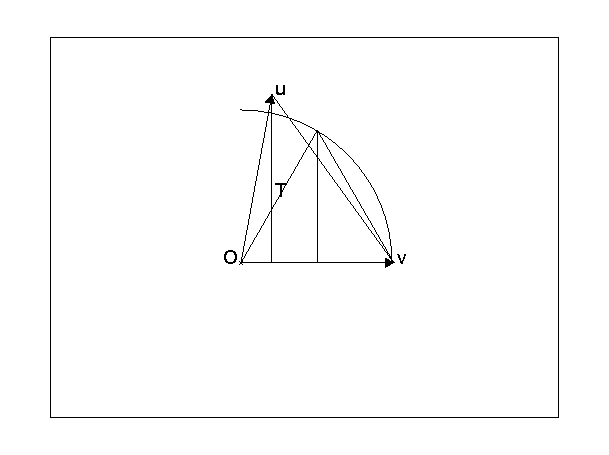
\includegraphics[width=8cm]{pa2b2}\\
Donc on a $(v*v)*\sqrt 3/2\leq p$ puisque :\\
pour tous les nombres $w$ du r\'eseau, on a $w*w$ est divisible par $p$ donc
si $v=(a,b)$ on a $v*v=a^2+b^2<2p$ et $v*v$ est un entier divisible par $p$ 
donc $v*v=a^2+b^2=p$.\\
{\bf Remarque}
Lorsque l'algorithme s'arr\^ete les vecteur $u$ et $v$ ont m\^eme norme et 
sont perpendiculaires.\\ 
En effet  lorsque l'algorithme s'arr\^ete on a :
\begin{enumerate}
\item $v*v=p$,
\item $|u*v|\leq v*v/2$ donc si $\alpha$ est l'angle form\'e par $u$ et $v$ on 
a : $\cos(\alpha)^2\leq 1/4$ ou $\sin(\alpha)^2\geq 3/4$,
\item $u*u$ est divisible par $p$ ($u*u=kp$ avec $k\in\N^*$) et $u*u\geq v*v$,
\item l'aire $A$ du parall\'elogramme engendr\'e par $u$ et $v$ vaut $p$
\item $v*v=p$
\end{enumerate}
Or $A^2=\sin(\alpha)^2(u*u)(v*v)=p^2=\sin(\alpha)^2(u*u)p$\\
Donc : $\sin(\alpha)^2(u*u)=p=\sin(\alpha)^2kp$\\
Donc : $k \sin(\alpha)^2=1\geq 3k/4$ avec $k\in\N^*$\\
Ou encore $k\in\N$ et $k\leq 4/3$ donc $k=1$ ce qui signifie que :\\
$u*u=p$ et  $\sin(\alpha)^2=1$ donc $u*v=0$\\
%pa2b2.xws
\end{itemize}
{\bf L'algorithme sur un exemple}\\
On choisit $p=13$, et prenons $rac =5$ (puisque $5^2=25=-1 \bmod 13$).\\
Dessinons quelques points du reseau en tapant :
\begin{verbatim}
reseau(p,rac):={
local L,j,k;
L:=NULL;
pour (j:=-2;j<=2;j++) {
  pour (k:=-3;k<=3;k++) {
    L:=L,point(k+i*(rac+k*p)+13*j);
  }
}
return affichage(L,epaisseur_point_2+1);
}:;
\end{verbatim}
%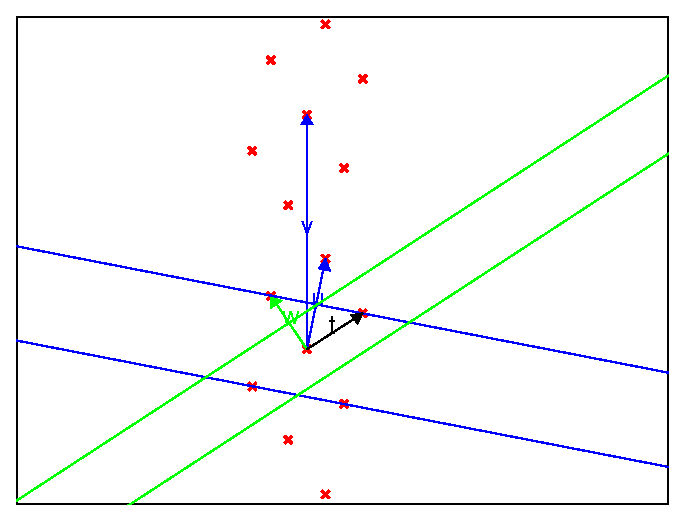
\includegraphics[width=\textwidth]{alga2b2}\\
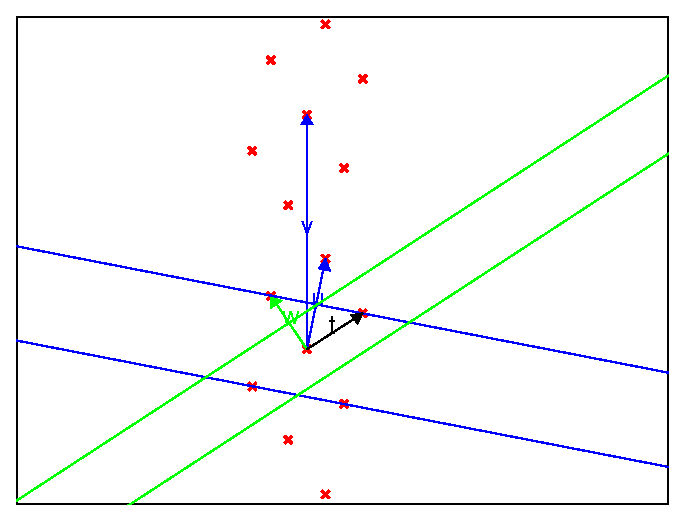
\includegraphics[width=11cm]{alga2b2}\\
On commence avec $u=1,rac$ et $v=0,p$. on r\'eduit $u,v$ ce qui veut dire 
que l'on \'echange $u$ et $v$ (car  $u*u<v*v$), puis on remplace $v$ par 
$w=v-2*u,u$ afin que $w$ soit dans la bande bleue.\\
On r\'eduit $w,u$ ce qui veut dire que l'on remplace $w,u$ par $u,w$ (car  
$u*u>w*w$) puis on remplace $u$ par $t=u-w$ afin que $t$ soit dans la bande 
verte. On s'arr\^ete et $t$ et $w$ sont de norme minimale ($t*t=w*w=2^2+3^2=13$).\\

{\bf L'algorithme}
\begin{enumerate}
\item On \'ecrit la fonction puissance rapide {\tt puiss(a,k,p)} qui renvoie
$a^k \bmod p$ (ou on utilise la fonction {\tt powmod} de {\tt Xcas}).
\item On \'ecrit la fonction {\tt sqrtmod(p)} qui renvoie une racine carr\'ee 
de -1 modulo $p$ lorsque $p$ est congru \`a 1 modulo 4.\\
Pour $p=13$, {\tt sqrtmod(13)} qui renvoie 8.

\item On \'ecrit la fonction {\tt reduire(u,v)} qui prend en entr\'ee deux 
vecteurs $u$ et $v$ de $\Z^2$, qui \'echange $u$ et $v$ si $v*v>u*u$ et renvoie 
$m,u1,v1$ tels que $-(v*v)/2<u+m*v\leq (v*v)/2$ (le produit \'etant le produit 
scalaire).\\
Pour $p=13$, {\tt reduire([1,8],[0,13])} renvoie {\tt -2,[-2,-3],[1,8]}, (car 
$[0,13]-2*[1,8]=[-2,-3]$)\\
{\tt reduire([-2,-3],[1,8])} renvoie {\tt 2,[-3,2],[-2,-3]} et\\
{\tt reduire([-3,2],[-2,-3])} renvoie {\tt 0,[-3,2],[-2,-3]}\\
ou si on a pris $rac=5$\\
{\tt reduire([1,5],[0,13])} renvoie {\tt -2,[-2,-3],[1,5]} et \\
{\tt reduire([-2,-3],[1,5])} renvoie {\tt -1,[-3,2],[-2,-3]} et \\
{\tt reduire([-3,2],[-2,-3])} renvoie {\tt 0,[-3,2],[-2,-3]}
\item On \'ecrit la fonction {\tt solpa2b2(p)} qui renvoie deux entiers $a$ et 
$b$ tels que $p=a^2+b^2$ lorsque $p$ est premier et congru \`a 1 modulo 4.\\
On it\`ere pour cela la fonction {\tt reduire} avec comme arguments initiaux 
$u=[1,sqrtmod(p)]$ et $v=[0,p]$ et on s'arr\^ete quand $m=0$.
On renvoie alors les coordonn\'ees en valeurs absolues du dernier $v$.
Pour $p=13$, {\tt solpa2b2(13)} renvoie $[3,2]$.
\end{enumerate}
{\bf Traduction de l'algorithme en langage {\tt Xcas}}
\begin{verbatim}
puiss(a,k,p):={
local pui;
pui:=1;
while(k>0) {
if (irem(k,2)!=0){
pui:=irem(a*pui,p);
k:=k-1;}
a:=irem(a*a,p);
k:=k/2;
}
return pui;
}:;
sqrtmod(p):={
local j,k,a,r;
if (!isprime(p)) {return p+"n'est pas premier"};
k:=iquo(p-1,4);
r:=irem(p-1,4);
if (r!=0) {return "erreur"};
a:=2;
j:=puiss(a,k,p);
while (j == 1 or j==p-1){
a:=a+1;
j:=puiss(a,k,p);
}
return j;
}:;
reduire(u,v):={
local w,uv,m,v2;
if (u*u<v*v){
w:=u;
u:=v;
v:=w;
}
uv:=u*v;
v2:=v*v;
m:=floor(1/2-uv/v2);
return m,u+m*v,v;
}:;
solpa2b2(p):={
local u,v,m,rac;
rac:=sqrtmod(p);
u:=[1,rac];
v:=[0,p];
m,u,v:=reduire(u,v);
while (m!=0) {
m,u,v:=reduire(u,v);
}
return abs(v);
}:;
\end{verbatim}
On tape :\\
{\tt solpa2b2(1009)}\\
On obtient :\\
{\tt [15,28]}\\
On tape :\\
{\tt pa2b2(1009)}\\
On obtient :\\
{\tt [28,15]}\\
On tape :\\
{\tt solpa2b2(1000033)}\\
On obtient :\\
{\tt [408,913]}\\
On tape :\\
{\tt pa2b2(1000033)}\\
On obtient :\\
{\tt [913,408]}\\
On tape :\\
{\tt solpa2b2(1000000009)}\\
On obtient :\\
{\tt [3747,31400]}\\
On tape :\\
{\tt pa2b2(1000000009)}\\
On obtient :\\
{\tt [31400,3747]}\\
On tape :\\
{\tt solpa2b2(1000000000061)}\\
On obtient :\\
{\tt [848494,529205]}\\
On tape :\\
{\tt pa2b2(1000000000061)}\\
On obtient :\\
{\tt [529205,848494]}
\section{Les nombres irr\'eductibles de $\Z[i]$}
\subsection{D\'efinitions et Th\'eor\`eme}
{\bf D\'efinition}\\
On dit que $a \in \Z[i]$ est {\bf inversible} si il existe $b \in \Z[i]$ 
tel que $ab=1$.\\
On dit que $b \in \Z[i]$ est {\bf associ\'e} \`a $a \in \Z[i]$ si il existe 
$c \in \Z[i]$ inversible tel que $a=bc$.\\
{\bf Exercice}\\
D\'eterminer les \'el\'ements inversibles de $\Z[i]$.\\
D\'eterminer les associ\'e de $x+iy \in \Z[i]$.\\
{\bf Solution}\\
Si  $a=a_1+ia_2 \in \Z[i]$ est inversible si il existe $b=b_1+ib_2 \in \Z[i]$ 
tel que $ab=1$.\\
Donc en \'egalant les modules :\\
$1=(a_1^2+a_2^2)(b_1^2+b_2^2)$ comme $a_1^2+a_2^2 \in \N$ et  
$b_1^2+b_2^2 \in \N$ cela entraine que $a_1^2+a_2^2=1$ c'est \`a dire
$a\in \{1,i,-1,-i\}$
Les associ\'es de $x+iy$ sont donc $\{x+iy,-x-iy,y+ix,y-ix\}$.\\
{\bf D\'efinition}\\
On dit que $a \in \Z[i]$ est {\bf irr\'eductible} si $a$ est non inversible ou 
si $a$ n'est le produit de 2 nombres appartenant \`a $\Z[i]$ que lorsque l'un 
de ces nombres est inversible.\\
Par exemple :\\
Les \'el\'ements inversibles de $\Z[i]$, $\{1,-1,i,-i\}$, ne sont pas 
irr\'eductibles dans $\Z[i]$.\\
2 n'est pas irr\'eductible dans $\Z[i]$ car $2=(1+i)*(1-i)$.\\
$1+2i$ est irr\'eductible car si $1+2i=(a_1+ia_2)(b_1+ib_2)$ alors en \'egalant
le carr\'e des modules on a :\\
$5=(a_1^2+a_2^2)(b_1^2+b_2^2)$. Comme 5 est premier cela entraine que 
$a_1^2+a_2^2=1$ (ou $b_1^2+_2^2=1$) c'est \`a dire
$a\in \{1,i,-1,-i\}$ (ou $b\in \{1,i,-1,-i\}$)\\
$(1+i)$ est irreductible car si $1+i=(a_1+ia_2)(b_1+ib_2)$ en \'egalant le
carr\'e des modules on obtient :\\
$2=(a_1^2+a_2^2)(b_1^2+b_2^2)$ donc
$(a_1^2+a_2^2)=1$ et $(b_1^2+b_2^2)=2$ (ou $(b_1^2+b_2^2)=1$ et 
$(a_1^2+a_2^2)=2$ ) ce qui veut dire que $(a_1+ia_2)$ est 
inversible et $(b_1+ib_2)$ est l'associ\'e de $1+i$ (ou
$(b_1+ib_2)$ est inversible et $(a_1+ia_2)$ est l'associ\'e de $1+i$).\\
{\bf Th\'eor\`eme}\\
Si dans $\Z[i]$ $a$ irr\'eductible divise $bc$ alors $a$ divise $b$ ou 
$a$ divise $c$.\\
{\bf Th\'eor\`eme}\\
Si un entier de Gauss est irr\'eductible alors l'un de ses associ\'e est :
\begin{enumerate}
\item le nombre $1+i$
\item $x+iy$ o\`u $x^2+y^2$ est un nombre premier de $\Z$  congru \`a 1 
modulo 4
\item un nombre premier de $\Z$ congru \`a 3 modulo 4
\end{enumerate}
Ainsi un entier de Gauss $z$ est irr\'eductible de type 1 ($z=1+i$), de type 2 
($z=x+iy$ o\`u $x^2+y^2$ est un nombre premier de $\Z$  congru \`a 1 
modulo 4) ou de type 3 ($z\in\Z$ avec $z$  congru \`a 3 modulo 4).\\
{\bf D\'emonstration}\\
Soit $a+ib$ un entier de Gauss est irr\'eductible
\begin{enumerate}
\item Supposons que $b=0$ alors $a+ib=p\in \Z$\\
Si $p$ est irr\'eductible, alors  $p$ est un nombre premier et $p$ peut \^etre :
\begin{itemize}
\item congru \`a 3 modulo 4.\\
Montrons qu'un nombre premier $p\in \Z$ congru \`a 3 modulo 4 est 
irr\'eductible dans $\Z[i]$.\\
Raisonnons par l'absurde et supposons que $p=(a_1+ia_2)(b_1+ib_2)$.\\
En \'egalant le carr\'e des modules on obtient :\\
$p^2=(a_1^2+a_2^2)(b_1^2+b_2^2)$
Comme $p$ est premier cela entraine que :\\
$a_1^2+a_2^2=p$ et que $(b_1^2+b_2^2)=p$
puisque $(a_1+ia_2)$ et $(b_1+ib_2)$ ne sont pas inversibles, on sait que 
$a_1^2+a_2^2\neq 1$ et $(b_1^2+b_2^2)=\neg 1$.\\
On a donc obtenu une contradiction puisque la somme de 2 carr\'es n'est jamais 
congru \`a 3 modulo 4.\\
Donc un nombre premier $p\in \Z$ congru \`a 3 modulo 4 est irr\'eductible dans
$\Z[i]$.\\
\item congru \`a 2 modulo 4.\\
Montrons qu'un nombre premier $p\in \Z$ congru \`a 2 modulo 4 n'est pas
irr\'eductible dans $\Z[i]$.\\
Comme $p$ est premier cela entraine que $p=2$.\\
Puisque $p=2=(1+i)*(1-i)$, $p$ n'est pas
irr\'eductible dans $\Z[i]$
\item congru \`a 1 modulo 4.\\
Montrons qu'un nombre premier $p\in \Z$ congru \`a 1 modulo 4 n'est pas
irr\'eductible dans $\Z[i]$.\\
On sait que si $p$ est un nombre premier congru \`a 1 modulo 4, il existe $a$ 
et $b$ dans $\N$ tels qie $p=a^2+b^2$ donc 
$p=(a+ib)*(a-i*b)$ donc $p$ n'est pas irr\'eductible.
\end{itemize}
\ \\
Donc si $p \in \Z$ est irr\'eductible dans $\Z[i]$ c'est que $p$ est premier
et congru \`a 3 modulo 4.

\item Soit un nombre $a+ib$ irr\'eductible dans  $\Z[i]$ avec $b\neq 0$ ou 
$a\neq 0$.
On en d\'eduit que $g=gcd(a,b)=1$ car sinon $a+i*b$ ne serait pas 
irr\'eductible car on aurait $(a+ib)=g*(a/g+ib/g)$.
Montrons tout d'abord que $p=a^2+b^2$ est un nombre premier de $\Z$ .\\
On a $p=a^2+b^2=(a+ib)(a-ib)$ avec $a+ib$ irr\'eductible dans  $\Z[i]$ donc
$(a+ib)$ divise $p_0$ un diviseur premier de $p$ dans $\Z$ .
Il existe donc il existe $c$ et $d$ dand $\N$ tels que :\\
$p_0=(a+ib)*(c+id)$ avec $c^2+d^2\neq 1$.\\
En \'egalant le carr\'e des modules on obtient :\\
$p_0^2=(a^2+b^2)(c^2+d^2)$ o\`u $p_0$ est un nombre premier de $\Z$
comme $c^2+d^2\neq 1$ et $(a^2+b^2)\neq 1$ (puisque $b\neq 0$ ou $a\neq 0$),  
on a  $p_0=a^2+b^2=c^2+d^2$.
 Donc si $a+ib$ est irr\'eductible dans  $\Z[i]$ avec $b\neq 0$ ou $a\neq 0$
alors $(a^2+b^2)$ est premier.\\
Donc $a^2+b^2$ est congru \`a 1 ou 2 modulo 4.\\
Si $a^2+b^2$ est congru \`a 2 modulo 4 c'est que $a^2+b^2=2$ (car $(a^2+b^2)$ 
est premier) et alors $a=1$ et $b=1$ sinon $a^2+b^2$ est congru \`a 1 modulo 4.
\end{enumerate}
{\bf Exercice}\\
\'Ecrire un programme {\tt estirreductible}, 
qui prend en entr\'ee un entier de Gauss $z$ et retourne son type (1, 2 ou 3)
si $z$ est irr\'eductble, et {\tt 0} sinon.
\begin{verbatim}
estirreductible(z):={
local p,m,n;
m:=abs(re(z));
n:=abs(im(z));
//if(type(m)!=2 or type(n)!=2){return faux; }:
if (z*conj(z)==1){return 0};
if (m==0) {m:=n;n:=0;}
if (n==0) {if (m>2 and irem(m-3,4)==0){return 3; }};
if (m==1 and n==1) {return 1; };
p:=m^2+n^2;
if (est_premier(p) and irem(p-1,4)==0){return 2; } else {return 0;} 
}
:;
\end{verbatim} 
{\bf Exercice}\\
\'Ecrire un programme qui d\'ecompose un entier de Gauss en un produit de
facteurs irr\'eductbles.
\begin{verbatim}
decompose(z):={
local p,L1,L2,L3,s2,s0,s1,s3,k,c,lc,fc,j,z1,d;
L1:=NULL;
L3:=NULL;
//if (im(z)==0) {p:=abs(z);} else {p:=z*conj(z);}
p:=z*conj(z);
L2:=ifactors(p);
s2:=size(L2);
c:=L2[0];
s0:=0;
if (c==2) {L1:=L1,1+i,,L2[1];s0:=2;z:=z/(1+i);}
for (k:=s0;k<s2;k:=k+2) {
c:=L2[k];d:=L2[k+1];
if (irem(c-1,4)==0) {
   lc:=pa2b2(c);
   fc:=lc[1]+i*lc[0];
   j:=0;z1:=z;
   while(irem(z1,fc)==0) 
     {j:=j+1;
       z1:=z1/fc;
      }
     if (j!=0 and j!=d) {
     L1:=L1,fc,j,conj(fc),d-j;
     z:=z/fc^j;z:=z/conj(fc)^(d-j);}
else {
    if (j==0) {L1:=L1,conj(fc),d;z:=z/conj(fc)^(d-j)}
else {L1:=L1,fc,j;z:=z/fc^j;}}
}
if (irem(c-3,4)==0) {L3:=L3,c,d/2;z:=z/c^(d/2);}
}
if (z==1){
 return [L1,L3];}
 else
{return [z,1,L1,L3];}
}
:;
\end{verbatim} 
Ou bien, on utilise la commande {\tt ifactors} ou la commande {\tt ifactor}.
\section{Les nombres d\'ecomposables}
{\bf D\'efinition}\\
On dit que $n \in \Z - \{-1,0,1\}$ est {\bf d\'ecomposable}, si pour tout 
diviseur premier $p$ de $1+n^2$ il existe $d\in \N$ v\'erifiant $d<abs(n)$ 
et tel que $1+d^2$ soit un multiple de $p$.\\
{\bf Par exemple}\\
8  est {\bf d\'ecomposable} car $1+8^2=65=5*13$ et on a 
5 divise $1+2^2=5$ ($d=2$) et 13 divise $1+5^2=26$ ($d=5$). \\
17  est {\bf d\'ecomposable} car $1+17^2=290=2*5*29$ et on a 
2 divise $1+1^2=2$ ($d=1$) et 5 divise $1+2^2=5$ ($d=2$) et 
29 divise $1+12^2=145=29*5$ ($d=12$). \\
6 est {\bf non d\'ecomposable}  car $1+6^2=37=1*37$ et on a 
1 divise $1+2^2=5$ ($d=2$) mais 37 ne divise pas $1+d^2$ quelque soit
$0\leq d\leq 5$ (car 37> $(1+d^2)$ lorsque $0\leq d\leq 5$).\\
19 est {\bf non d\'ecomposable}  car $1+19^2=362=2*181$ et on a 
2 divise $1+3^2=10$ ($d=2$) mais 181 ne divise pas $1+d^2$ quelque soit
$0\leq d\leq 18$ (car 180 n'est pas un carr\'e).\\
{\bf Exercice}\\
\'Ecrire une fonction {\tt Xcas} {\tt estdecomposable}, 
qui prend en entr\'ee un entier $n$, et retourne le bool\'een {\tt vrai}
si $n$ est d'ecomposable, {\tt faux} sinon.\\
Et v\'erifier que les premiers entiers d\'ecomposables sont :\\
{\tt 3,7,8,12,13,17,18,21,23,27,30}\\
\ \\
Les diff\'erentes solutions avec des algorithmes de plus en plus performents.
\begin{itemize}
\item{\bf Algorithme 0}\\
L'{\bf Algorithme 0} est un algorithme naif qui pour tout diviseur premier
de $1+n^2$ cherche l'existence de $d$ par balayage (la variable $t$ sert de 
test ). Avec cet algorithme, si $n$ est d\'ecomposable on trouve le plus petit 
entier $d$ : 
\begin{verbatim}
estdeconposable0(n):={
local p,Lf,k,p1,d,t,s;
n:=abs(n);
p:=1+n^2;
if (isprime(p)) {return faux};
Lf:=ifactors(p);
s:=size(Lf);
for (k:=0;k<s;k:=k+2){
p1:=Lf[k];
d:=1;
t:=0;
while(t!=1 and d<n) {
if (irem(1+d^2,p1)==0) {t:=1;afficher(d,p1);};
d:=d+1;
}
if (t==0){return faux;}
}
return vrai;
}:;
\end{verbatim} 
\item{\bf Algorithme 1}\\
L'{\bf Algorithme 1} va faire appel aux nombres complexes.\\
$N=1+n^2$ est la norme au carr\'ee de $z=1+i*n$ et soit $p$ un diviseur premier
de $N$.\\
Donc $p$ divise $(1+in)(1-in)$.\\

\begin{itemize}
\item $p$ n'est pas congru \`a 3 modulo 4.\\
 En effet si $p$ est congru \`a 3 modulo 4, $p$ est irr\'eductible dans $\Z[i]$
donc $p$ divise $1+in$ ou $1-in$. Cela veut dire qu'il existe $x \in \Z$ et 
$y \in \Z$ tel que $p(x+iy)=1+in$ (ou $p(x+iy)=1-in$) ce qui est impossible car 
$p$ diviserait 1 puisqu'en \'egalant les parties r\'eelles on a $p*x=1$
\item
$p$ n'est pas congru \`a 0 modulo 4 car $p$ est premier
\item $p=2$ ou $p$ est congru \`a 1 modulo 4
En effet si $p$ est congru \`a 2 modulo 4 c'est que $p=2$ car $p$ est premier
\end{itemize}
On sait que tout nombre premier $p$ congru \`a 1 modulo 4 est la somme des
carr\'es de 2 entiers  donc il existe $a\in \N$ et $b\in N$:\\
$p=a^2+b^2$.\\
On cherche les entiers $d$ qui sont tels que :\\
$p=a^2+b^2=(a+i*b)(a-i*b)$ divise $1+d^2=(1+i*d)(1-i*d)$ donc \\
on cherche les entiers $d \in Z$ qui sont tels que :\\
$a+i*b$ divise $1+i*d$ c'est \`a dire tel qu'il existe $u$ et $v$ v\'erifiant :\\
$(a+ib)(u+iv)=1+i*d$\\
donc $au-bv=1$ et $av+bu=d$\\
Tous les $d$ sont congrus modulo $p=a^2+b^2$ (car si $au0-bv0=1$ et
$au-bv=1$ alors $u=u0+k*b$ et $v=v0+k*a$)\\
\begin{verbatim}
estdecomposable1(n):={
local p,N,Lf,k,d,d1,a,b,L,a1,b1,s;
n:=abs(n);
N:=1+n^2;
if (isprime(N)) {return faux};
Lf:=ifactors(N);
s:=size(Lf);
for (k:=0;k<s;k:=k+2){
p:=Lf[k];
if (p!=2){
//on irem(p,4)==1 et p premier
a,b:=pa2b2(p);
if (a!=1 and b!=1) {
L:=iegcd(a,b);
a1:=L[0];
b1:=-L[1];
d:=irem(b*a1+a*b1,p);
d1:=irem(-b*a1-a*b1,p);
//afficher(d,d1,p);
};
if (d>=n et d1>=n) {return faux;}
}
}
return vrai;
}:;
\end{verbatim} 
\item {\bf Algorithme 2}\\
l'{\bf Algorithme 2} simplifie l'algorithme1 puisque  $n$ et $-n$ se trouve 
\^etre un $d$ particuler, donc  le plus petit $d$ est \'egal 
\`a $n \bmod p$ ou \`a $-n \bmod p$.
\begin{verbatim}
estdecomposable2(n):={
local p,N,Lf,k,d,a,b,d1,s;
n:=abs(n);
N:=1+n^2;
if (isprime(N)) {return faux};
Lf:=ifactors(N);
s:=size(Lf);
for (k:=0;k<s;k:=k+2){
p:=Lf[k];
if (p!=2){
d:=irem(n,p);
d1:=irem(-n,p);
afficher(d,d1,p);}
if (d1>=n et d >=n){return faux;}
}
}
return vrai;
}:;
\end{verbatim} 
\item {\bf Algorithme}\\
L'{\bf Algorithme} (le bon !!!!) utilise le th\'eor\`me suivant :\\
{\bf Th\'eor\`eme 1}:\\
Si $p$ est premier et est congru \`a 1 modulo 4 alors il existe $a$ et $b$ tel 
que $p=a^2+b^2$ et il existe $u+iv$ unique tel que :\\
$(a+ib)(u+iv)=1+im$ avec $m\in \Z$, $abs(m)<p/2$ et $u^2+v^2\leq 0.29p$\\
Cela entraine que si $p$ est premier et congru \`a 1 modulo 4 alors il existe 
$m \in \Z$ tel que $p$ divise $1+m^2$ et $m$ est unique dans $]-p/2;p/2[$.\\

{\bf D\'emonstration}\\
Soit $p\in \N$ un nombre premier congru \`a 1 modulo 4 il existe $a$ et $b$ 
tel que $p=a^2+b^2$.\\
On cherche $u, v,m \in \Z^3$ de valeur absolue la plus petite possible tels 
que :  \\
$(a+ib)(u+iv)=1+im$\\
on a donc :\\
$au-bv=1$ et $av+bu=m$.
Puisque $p=a^2+b^2$ est premier $a$ et $b$ sont premier entre eux donc il 
existe $u$ et $v$ (identit\'e de B\'ezout) tels que :\\
$au-bv=1$ et les solutions sont de la forme :\\
$u=u_0+kb v=v_0+ka \ k\in \Z$ o\`u $u_0,v_0$ est une solution 
particuli\`ere de $au-bv=1$.\\
On a donc :\\
$(a+ib)(u0+iv0+k(b+ia))=1+im$\\
$(a+ib)(u0+iv0)+ik(a^2+b^2)=1+im$\\
Donc  : $m=av_0+bu_0+k(a^2+b^2) \ k\in \Z$ c'est \`a dire les $m$ solutions 
sont \`egaux modulo $p$.\\
Comme $a^2+b^2=p$ est impair on en d\'eduit qu'il existe un $m_0$ et un seul 
tel que $|m_0|<p/2$ ($m \in \{(1-p)/2,..-1,0,1... (p-1)/2 \}$).\\
Comme $(a+ib)(u+iv)=1+im_0$, on a $(a^2+b^2)(u^2+v^2)=1+m_0^2=p(u^2+v^2)$
Puisque $p$ est un nombre premier  congru \`a 1 modulo 4, on a $p\geq 5$ donc
$p^2\geq 25$ ou encore $1/p\leq p/25$ donc :\\
$p(u^2+v^2)=1+m_0^2<1+p^2/4$  donc \\
$(u^2+v^2)\leq 1/p+p/4<p/25+p/4=0.29p$\\
On tape :
\begin{verbatim}
estdecomposable(n):={
local p,N,Lf,k,d,d1,s,s1;
n:=abs(n);
N:=1+n^2;
if (isprime(N)) {return faux};
Lf:=ifactors(N);
s:=size(Lf);
p:=Lf[0];
if (p==2){s1:=2} else {s1:=0};
for (k:=s1;k<s;k:=k+2){
p:=Lf[k];
//on a irem(p,4)==1 et p premier
if (abs(n)<p/2) {return faux;}
}
return vrai;
}:;
\end{verbatim} 
\end{itemize}
On tape pour avoir la liste des nombres d\'ecomposables plus petit que $n$ :
\begin{verbatim}
Lestdecomposable(n):={
local L,k;
L:=NULL;
for (k:=1;k<=n;k++){
if (estdecomposable(k)) {
L:=L,k;
}
}
return L;
}:;
\end{verbatim} 
{\tt Lestdecomposable(35)}\\
On obtient :\\
{\tt 3,7,8,13,17,18,21,30,31,32}
\section{Les nombres compl\'etables}
{\bf Definition} :\\
On dit que le nombre $z=a+ib$ est compl\'etable si il existe $u+iv \in \Z[i]$ 
 et $m\in \Z$ tel que : $(a+ib)(u+iv)=1+im$ .\\
{\bf Th\'eor\`eme2} :\\
Si $a$ et $b$ sont premiers entre eux alors $z=a+ib$ est compl\'etable.
De plus,  si $a\neq 1$ et $b\neq 1$, il existe $u,v,m \in \Z^3$  uniques tel 
que $(a+ib)(u+iv)=1+im$ et $|m|<(a^2+b^2)/2$ et $u^2+v^2<0.29(a^2+b^2)$.\\
De plus $u$ et $v$ sont premiers entre eux et donc $u+iv$ et $u-iv$ sont
compl\'etables.\\
{\bf D\'emonstration}\\
C'est le th\'eor\`eme1 sans l'hypoth\`ese $p=a^2+b^2$ premier.\\
Tout d'abord $1+in$ et $n+i$ sont compl\'etables car $(1+in)*1=1+in$ et 
$(n+i)*(-i)=1-in$ et on a $n<(1+n^2)/2$ si et seulement si $n\neq 1$.\\
Soient $a\neq 1$ et $b\neq 1$ premiers entre eux et $z=a+ib$.\\
On suppose donc que $a^2+b^2\geq 5$.\\
On a vu (cf th 1) que les $m$ v\'erifiant $(a+ib)(u+iv)=1+im$ sont congru 
modulo $a^2+b^2$.\\
On va consid\'erer 2 cas :
\begin{itemize}
\item $a^2+b^2$ est impair i.e. $a^2+b^2=2q+1$\\
il existe donc un $m$ unique dans $\{-q,-q+1...-1,0,1,..q\}$ donc\\
$m\leq q<q+1/2=(a^2+b^2)/2$
\item $a^2+b^2$ est pair i.e. $a^2+b^2=2q$ et $q>2\\$
il existe donc un $m$ unique dans $\{-q+1...-1,0,1,..q\}$.\\
Mais on ne peut pas avoir $m=q$ car alors  on aurait :\\
$(a^2+b^2)(u^2+v^2)=2q(u^2+v^2)=1+q^2$ donc $q$ diviserait 1.\\
Donc il existe un $m$ unique dans $\{-q+1...-1,0,1,..q-1\}$ donc :\\
$m\leq q-1<q=(a^2+b^2)/2$.
\end{itemize}
Puisque $a^2+b^2\geq 5$ on a $(a^2+b^2)^2\geq 25$ ou encore :\\
$1/(a^2+b^2)\leq (a^2+b^2)/25$ donc :\\
$(a^2+b^2)(u^2+v^2)=1+m^2<1+(a^2+b^2)^2/4$ donc \\
$(u^2+v^2)< 1/(a^2+b^2)+(a^2+b^2)/4\leq (1/25+1/4)(a^2+b^2)=0.29(a^2+b^2)$.\\

Le programme {\tt complete} ci-dessous a comme argument $z=a+in$ et
renvoie $u+iv,1+im$ avec 
$(a+ib)(u+iv)=1+im\ $  et $\ -(a^2+b^2)/2<m<(a^2+b^2)/2$
\begin{verbatim}
complete(z):={
local p,m,a,b,u,v,L;
a:=re(z);
b:=im(z);
p:=a^2+b^2;
if (gcd(a,b)!=1){ return faux;}
if (a==1) {return 1,1+i*b};
if (b==1) {return -i,1-i*a};
L:=iegcd(a,b);
u:=L[0];
v:=-L[1];
m:=irem(b*u+a*v,p);
if (m>p/2){m:=m-p;}
return u+i*v,1+i*m;
}:;
\end{verbatim}
Si on veut une liste des nombres qui compl\'etent le nombre compl\'etable 
$a+ib$, on tape :
\begin{verbatim}
Lcomplete(z):={
local L,z1,a1,b1,d1,k,b,a ;
L:=complete(z);
z1:=L[0];
a1:=re(z1);
b1:=im(z1);
a:=re(z);
b:=im(z);
d1:=L[1];
return ([a1+k*b+i*b1+i*k*a,d1+i*k*abs(z)^2])$(k=-5..5);
}:;
\end{verbatim}
\section{L'algorithme de Todd}\label{sec:Todd}
\subsection{Le Th\'eor\`eme3}
Soit $n\geq 2$ un entier d\'ecomposable (i.e. pour tout diviseur premier $p$ de 
$1+n^2$ et il existe $d$,  $0<d<n$, tel que $p$ soit aussi un diviseur 
premier de $1+d^2$).\\
Il existe un entier $M>1$ et des entiers $w_j$ ($|w_j|<n$) tels que :\\
$M(1+in)=\epsilon(1+iw_1)^{a_1}(1+iw_2)^{a_2}...(1+iw_k)^{a_k}$ ($\epsilon \in \{1,-1,i,-i\}$).\\
Cette formule donne en \'egalant les arguments :\\
$\atan(n)=arg(\epsilon)+\sum_{j=1}^ka_j\atan(w_j)+m\pi$.\\
et puisque pour $x>0$ on a :\\
$\atan(x)+\atan(1/x)=\pi/2$\\
on a aussi :\\
$\atan(1/n)=-arg(\epsilon)+\sum_{j=1}^k\atan(1/w_j)+q*\pi$.\\

Soit $n\geq 2$ un entier d\'ecomposable. L'algorithme de Todd factorise
$1+in$ et compl\'ete par $u+iv$ chaque facteur irr\'eductible $a+ib$ si 
$a\neq 1$ ou $b\neq 1$ pour avoir $(a+ib)(u+iv)=1+im$\\
Par exemple si $(1+in)=(a+ib)*z1$, on obtient :\\
$(1+in)(u+iv)(u-iv)=(a+ib)(u+iv)(u-iv)z1$  donc\\
$(1+in)(u^2+v^2)=(1+im)(u-iv)z1$\\
Si $u==1$ ou $v==1$ on s'occupe d'un autre facteur irr\'eductible, sinon
on compl\'ete $(u+iv)$....\\
Comme $(u^2+v^2)<0.29(a^2+b^2)$ $u^2+v^2$ diminue \`a chaque compl\'etion, donc 
l'algorithme s'arr\^ete.\\
\subsection{Un Exemple} 
On va montrer sur un exemple comment fonctionne l'algorithme de Todd.\\
Soit $n=342$ $n$ est d\'ecomposable.\\
On tape :\\
{\tt ifactors(1+i*342)}\\
On obtient :\\
{\tt [-1,1,2-i,1,10-7*i,1,11-6*i,1]}\\
On a : $-(2-i)=-2+i=i(1+2i)$\\
Donc $1+342i=i(1+2i)(10-7i)(11-6i)$\\
On tape :\\
{\tt complete(10-7*i)}\\
On obtient :\\
{\tt -2+3*i,1+44*i}\\
donc $(10-7i)*(-2+3i)=1+44i$\\
On tape :\\
{\tt complete(-2-3*i)}\\
On obtient :\\
{\tt 1+i,1-5*i}\\
donc \\
$(10-7i)(-2+3i)(-2-3i)(1+i)(1-i)=26(10-7i)=(1+44i)(1-5i)(1-i)$\\
On tape :\\
{\tt complete(11-6*i)}\\
On obtient :\\
{\tt -1+2*i,1+28*i}\\
donc $(11-6*i)(-1+2i)=1+28i$\\
donc $(11-6*i)(-1+2i)(-1-2i)=5(11-6*i)=(1+28i)(-1-2i)$\\
Donc puisque $-(2-i)=i(1+2i)$ on a :\\
$5*26(1+342i)=i(1+2i)(1+44i)(1-5i)(1-i)(1+28i)(-1-2i)$\\
$130(1+342i)=-i(1-i)(1+2i)^2(1-5i)(1+28i)(1+44i)$
\subsection{Exercice}
\begin{enumerate}
\item Soit $f(x)=\atan(x)+\atan(\frac{1}{x})$.\\
D\'eterminer le domaine de d\'efinition de $f$.\\
Calculer $f'(x)$ puis montrer que :
$$\atan(x)+\atan(\frac{1}{x})=\frac{\pi}{2} \mbox{ si} x>0$$
$$\atan(x)+\atan(\frac{1}{x})=-\frac{\pi}{2} \mbox{ si} xx0$$
\item Soit $g(x)=\atan(\frac{x+a}{1-ax})-\atan(x)$ pour $a\in \R$
D\'eterminer le domaine de d\'efinition de $g$.\\
Calculer $g'(x)$ puis montrer que :\\
si $ab<1$ alors $\atan(a)+\atan(b)=\atan((a+b)/(1-ab))$ et \\
si $ab=1$ et $a>0$ alors $\atan(a)+\atan(b)=\pi/2$ et\\
si $ab=1$ et $a<0$ alors $\atan(a)+\atan(b)=-\pi/2$.\\
si $ab>1$ et $a>0$ alors $\atan(a)+\atan(b)=\pi+\atan((a+b)/(1-ab))$ et\\
si $ab>1$ et $a<0$ alors $\atan(a)+\atan(b)=-\pi+\atan((a+b)/(1-ab))$.
\item En d\'eduire que :\\
$\atan(28)+\atan(44)=\pi+\atan(-72/1231)$\\
$2\atan(2)+\atan(-5)=\pi+\atan(-4/3)+\atan(-5)=\atan(19/17)$\\
$\pi+\atan(-72/1231)+\atan(19/17)=\pi+\atan(341/343)$ donc\\
$atan(-1)+2\atan(2)-\atan(5)+\atan(28)+\atan(44)=\pi+atan(-1)+\atan(341/343)=$\\
$\pi-\atan(1/342)=\pi/2+\atan(342)$\\
Donc puisque $\atan(-1)=-\pi/4$ et puisque pour $x>0$ on a :\\
$\atan(x)+\atan(1/x)=\pi/2$ on obtient :\\
$\atan(342)=-3\pi/4+2\atan(2)-\atan(5)+\atan(28)+\atan(44)$\\
Donc puisque pour $x>0$ on a $\atan(x)+\atan(1/x)=\pi/2$\\
$\atan(1/342)=-\pi/4+2\atan(1/2)-\atan(1/5)+\atan(1/28)+\atan(1/44)$
\end{enumerate}
\subsection{Un programme qui simplie les formules pr\'ec\'edentes}
On peut \'ecrire un petit programme {\tt ajuste} pour simplifier :
$\sum_{j=1}^ka_j\atan(w_j)$.\\
{\tt ajuste} a comme argument la liste form\'ee par les arguments $w_j$ des 
arcs tangentes  en r\'ep\'etant $a_j$ fois $w_j$ et renvoie {\tt C,a} 
tel que :\\
$\sum_{j=1}^ka_j\atan(1/w_j)=C+\atan(a)$.\\
Par exemple pour la formule :\\
$\atan(-1)+2\atan(2)-\atan(5)+\atan(28)+\atan(44)$.
on met comme argument la liste {\tt L:=[-1,2,2,-5,28,44]} et {\tt ajuste(L)}
 renvoie {\tt pi,-1/342}.\\
On d\'efinit $f$ la fonction $f$ par :\\
{\tt f(a,b):=(a+b)/(1-a*b);}\\
Pour simplifier $\atan(a)+\atan(b)$, on \'ecrit tout d'abord la fonction 
{\tt simpl(a,b)} qui renvoie {\tt C,c} tel que :\\
$\atan(a)+\atan(b)=C+\atan(c)$\\
Puis,   on \'ecrit {\tt ajuste(L)} qui renvoie {\tt C,c} tel que :\\
$\sum_j\atan(L[j])=C+\atan(c)$
\begin{verbatim}
f(a,b):=(a+b)/(1-a*b);
simpl(a,b):={
local s;
if (a==0) {return 0,b;}
if (b==0) {return 0,a;}
s:=sign(a);
if (a*b==1) {return s*pi/2,0;}
if  (a*b<1) {return 0,f(a,b);}
if  (a*b>1) {return s*pi,f(a,b);}
}:;
ajuste(L):={
local s,a,b,C,c,ajou,k;
ajou:=0;
s:=size(L);
a:=L[0];
k:=1;
while (k<s){
b:=L[k];
C,c:=simpl(a,b);
ajou:=ajou+C;
a:=c;
k:=k+1;
}
return normal(ajou),a;
}:;
\end{verbatim} 
On tape : {\tt ajuste([-1,2,2,-5,28,44])}\\
On obtient : {\tt pi,-1/342}\\
Donc :\\
$\atan(342)+\pi/2=\atan(-1/342)+\pi=\atan(-1)+2*\atan(1/2)-\atan(1/5)+\atan(1/28)+\atan(1/44)$\\
Donc :\\
$\atan(342)=-\pi/2+\atan(-1)+2*\atan(2)-\atan(5)+\atan(28)+\atan(44)$\\
On tape : {\tt ajuste([-1,1/2,1/2,-1/5,1/28,1/44])}\\
On obtient : {\tt 0,1/342}\\
Donc :\\
$\atan(1/342)=\atan(-1)+2*\atan(1/2)-\atan(1/5)+\atan(1/28)+\atan(1/44)$\\

{\bf Remarque}\\
En utilisant {\tt Lcomplete(11-6*i)} on voit que:\\
$(11-6i)(5-9i)=1-129i$ \\
On peut aussi utiliser cette compl\'etion car $123<342/2$ et 
$5^2+9^2=106<342/3$.\\
On tape :\\
{\tt complete(5+9i)}\\
On obtient :\\
{\tt 2+i,1+23*i}\\
Donc $(5+9i)(2+i)=1+23i$\\
Donc on a :\\
$(11-6i)(5-9i)(5+9i)(2+i)(2-i)=5*106(11-6i)=(1-129i)(1+23i)(2-i)$\\
On obtient alors :\\
$1+342i=i(1+2i)(10-7i)(11-6i)$\\
$5*106*26(1+342i)=i(1+2i)(1+44i)(1-5i)(1-i)(1-129i)(1+23i)(2-i)$\\
$13780(1+342i)=(1-i)(1+2i)^2(1-5i)(1+23i)(1+44i)(1-129i)$\\
Donc :\\
$\atan(342)=-\pi/4+2\atan(2)-\atan(5)+\atan(23)+\atan(44)-\atan(129)$\\
Donc puisque pour $x>0$ on a $\atan(x)+\atan(1/x)=\pi/2$ on a :\\
$\atan(1/342)=-\pi/4+2\atan(1/2)-\atan(1/5)+\atan(1/23)+\atan(1/44)-\atan(1/129)$\\
On tape : {\tt ajust([-1,2,2,-5,23,44,-129])}\\
On obtient : {\tt 0,1/342}\\
On tape : {\tt ajust([-1,1/2,1/2,-1/5,1/23,1/44,-1/129])}\\
On obtient : {\tt 0,-342}\\
{\bf Traduction de l'algorithme de Todd en langage {\tt Xcas}}\\
\begin{verbatim} 
todd(n):={
 local L,k,s,s1,z,R,Z,Zc,zc,p;
 //if (estcompletable(n)==faux) {return faux;};
 L:=ifactors(1+i*n);
 s:=size(L);
 R:=NULL;
 p:=1;
 for (k:=2;k<s;k:=k+2){
  z:=L[k];
  if (im(z)^2==1 or re(z)^2==1) {
    R:=R,z,L[k+1];}
  else {
    Z:=complete(z);
    R:=R,Z[1],L[k+1];
    zc:=conj(Z[0]);
    p:=p*abs(zc)^(2*L[k+1]);
    while (re(zc)^2!=1 and im(zc)^2!=1){
      Zc:=complete(zc);
      R:=R,Zc[1],L[k+1];
      zc:=conj(Zc[0]);
      p:=p*abs(zc)^(2*L[k+1]);
    }
    R:=R,zc,L[k+1];
  }
 }
 return normal(p),[L[0],1,R];
}:;
\end{verbatim}
On tape :\\
{\tt todd(342)}\\
On obtient :\\
{\tt 130,[-1,12-i,1,1+44*i,1,1-5*i,1,1-i,1,1+28*i,1,-1-2*i,1]}\\
On tape :\\
{\tt todd(266)}\\
On obtient :\\
{\tt 1850,[i,1,1-80*i,1,1+6*i,1,1-143*i,1,-1+7*i,1]}
\section{Pour obtenir une formule de type Machin}
Une formule de type Machin est une formule qui ressemble \`a :
$$\atan(1/n)=k*\pi+\sum_{j=0}^ka_j\atan(1/wj)$$ avec $0<wj<n$
Si le but est d'obtenir une formule avec des arcs tangentes, on modifie 
l'algorithme pr\'ec\'edent pour avoir seulement comme r\'esultat la liste des 
$w_j$ compt\'e avec leur multiplicit\'e.\\
On tape :
\begin{verbatim} 
todd2(n):={
local L,k,s,s1,z,R,Z,Zc,zc,p,RR;
//if (estcompletable(n)==faux) {return faux;};
L:=ifactors(1+i*n);
s:=size(L);
R:=NULL;
p:=1;
for (k:=2;k<s;k:=k+2){
z:=L[k];
if (im(z)^2==1 or re(z)^2==1) {R:=R,z,L[k+1];}
else {Z:=complete(z);
R:=R,Z[1],L[k+1];
zc:=conj(Z[0]);
p:=p*abs(zc)^(2*L[k+1]);
while (re(zc)^2!=1 and im(zc)^2!=1){
Zc:=complete(zc);
R:=R,Zc[1],L[k+1];
zc:=conj(Zc[0]);
p:=p*abs(zc)^(2*L[k+1]);
}
R:=R,zc,L[k+1];
}
}
RR:=NULL;
s:=size(R);
for (k:=0;k<s;k:=k+2){
if (re(R[k])^2!=1){R[k]:=i*R[k];}
RR:=RR,(re(R[k])*im(R[k]))$(R[k+1]);
}
return sort(RR);
}
:;
\end{verbatim}
On tape :\\
{\tt todd2(342)}\\
On obtient :\\
{\tt -5,-1,2,2,28,44}\\
On tape :\\
{\tt ajust(todd2(342))}\\
On obtient :\\
{\tt 0,1/266}\\
Donc :\\
$\atan(1/342)=\atan(-1/5)+\atan(-1)+2\atan(1/28)+\atan(1/44)$\\
On tape :\\
{\tt todd2(266)}\\
On obtient :\\
{\tt -143,-80,-7,6}\\
On tape :\\
{\tt ajust(todd2(266))}\\
On obtient :\\
{\tt 0,1/266}\\
Donc :\\
$\atan(1/266)=\atan(-1/143)+\atan(-1/80)+\atan(-1/7)+\atan(1/6)$

\chapter{Pour s'amuser avec le tableur de {\tt Xcas}}
\section{Nombre de carr\'es dans un \'echiquier}
On cherche le nombre de carr\'es $NC(n)$ que l'on peut former sur un \'echiquier
de dimension $n*n$.\\
On veut faire une fiche de travail pour que les \'el\`eves devine et d\'emontre
que :\\
$$NC(n)=1^2+2^2+3^2+...+n^2=\frac{n(n+1)(2n+1)}{6}$$
\subsection{L'\'enonc\'e}
On rappelle que $1+2+...n=\frac{n(n+1)}{2}$.
\begin{enumerate}
\item Combien peut-on former de carr\'es de c\^ot\'es \'egal \`a 1 sur un 
\'echiquier de dimension $p*p$ ?
\item Combien peut-on former de carr\'es de c\^ot\'es \'egal \`a $n$ sur un 
\'echiquier de dimension $n*n$ ?
\item Expliquer pourquoi le nombre de carr\'es de c\^ot\'es \'egal \`a $n-1$ 
sur un \'echiquier de dimension $n*n$ est \'egal au nombre de carr\'es de 
c\^ot\'es \'egal \`a 1 sur un \'echiquier de dimension $2*2$.
\item  Expliquer pourquoi le nombre de carr\'es de c\^ot\'es \'egal \`a $n-2$ 
sur un \'echiquier de dimension $n*n$ est \'egal au nombre de carr\'es de 
c\^ot\'es \'egal \`a 1 sur un \'echiquier de dimension $3*3$?
\item Sur le tableur de {\tt Xcas} remplir :
\begin{itemize}
\item la premi\`ere colonne avec les nombres de 0 \`a $n$ (par exemple $n=39$).
\item la deuxi\`eme colonne avec le nombre de carr\'es de c\^ot\'es \'egal \`a 
1, sur un \'echiquier de dimension $p*p$ ($p=1..n$) qui est aussi le nombre de 
carr\'es de dimension $n-p+1$ sur un \'echiquier de dimension $n*n$.
\item la troisi\`eme colonne avec avec les sommes partielles de la deuxi\`eme 
colonne. Dire pourquoi cette colonne donne $NC(k)$ lorsque $A(k)=k$.
\item la quatri\`eme colonne avec les sommes partielles de la premi\`ere 
colonne.
\item la cinqui\`eme colonne  avec le quotient de la  la troisi\`eme colonne
par la  quatri\`eme colonne.
\item Deviner l'expression de la cinqui\`eme colonne et en d\'eduire 
la valeur de l'expression de $NC(n)$.
\end{itemize}
\end{enumerate}
\subsection{La correction avec {\tt Xcas}}
\begin{enumerate}
\item On a $0,1,2,3..n$ sur la colonne $A$
\item On a $0,1,4,9...n^2$ sur la colonne $B$
\item On a $0,1,5,14,30....$ sur la colonne $C$
\item On a $0,1,3,6,10,15....$ sur la colonne $D$ c'est \`a dire $k(k+1)/2$
pour $k=1..n$. Donc $D(k)=1^2+2^2+...k^2=NC(k)$. 
\item On a $0,1,5/3,7/3,3,11/3,13/2,5....$ sur la colonne $E$.\\
On devine que la colonne $E$ vaut $(2k+1)/3$ pour $k=1..n$.\\
Puisque la colonne $D$ vaut $k(k+1)/2$ pour $k=1..n$, on en d\'eduit que
$NC(k)=k(k+1)/2*(2k+1)/3=k(k+1)(2k+1)/6$.\\
On peut maintenant montrer par r\'ecurrence que :
$$1^2+2^2+...k^2=\frac{k(k+1)(2k+1)}{6}$$ car\\
$1^2=(1*2*3)/6$ et\\
$$ 1^2+...k^2+(k+1)^2=\frac{(k+1)(2k^2+k+6k+6)}{6}=\frac{(k+1)(k+2)(2k+3)}{6}$$
\end{enumerate}

\section{\'Etude d'une suite}
\subsection{L'\'enonc\'e}
On consid\`ere la suite r\'ecurrente :\\
$u_0=a$\\
$u_1=b$\\
pour $n>1$ $u_n=|u_{n-1}|-u_{n-2}$\\
\'Etudiez cette suite.\\
Faites des essais avec le tableur prendre par exemple :\\
$a=3$ avec $b=4, b=5,b=7$ etc...\\
$a=-3$ avec $b=4, b=5,b=7$ etc...\\
Que remarquez-vous ?\\

\subsection{La d\'emarche math\'ematique}
On va montrer que cette suite est p\'eriodique ($u_9=u_0$ et $u_{10}=u_1$).\\
Pour cela on consid\`ere 9 cas :\\
6 cas lorsque $b>=0$ et 3 cas lorsque $b<0$:\\
{\bf cas 1} : $b \geq 2a \geq 0$\\
On obtient :\\
{\tt a,b,b-a,-a,-b+2a,b-a,2b-3a,-2a+b,a-b,a,b....}\\
{\bf cas 2} : $2a > b \geq a$\\
On obtient :\\
{\tt a,b,b-a,-a,-b+2a,3a-b,a,2a+b,a-b,a,b.....}\\
{\bf cas 3} : $a/2 >b \geq 0$\\
On obtient :\\
{\tt a,b,b-a,a-2b,-3b+2a,a-b,2b-a,-b,-b+a,a,b....}\\
{\bf cas 4} : $a>  b \geq a/2$\\
On obtient :\\
{\tt a,b,b-a,a-2b,b,3b-a,2b-a,-b,a-b,a,b...}\\
{\bf cas 5} : $b \geq -a \geq 0$\\
On obtient :\\
{\tt a,b,b-a,-a,-b,b+a,2b+a,b,b-a,a,b....}\\
{\bf cas 6} : $-a \geq b \geq 0$\\
On obtient :\\
{\tt a,b,b-a,-a,-b,b+a,-a,-2a-b,-a-b,a,b....}\\
{\bf cas 7} : $-b \geq a >0$\\
On obtient :\\
{\tt a,b,-b-a,-2b-a,-b,b+a,-a,-b,-b+a,a,b....}\\
{\bf cas 8} : $a >-b >0$\\
On obtient :\\
{\tt a,b,-b-a,a,2a+b,a+b,-a,-b,-b+a,a,b....}\\
{\bf cas 9} : $-b >0 \geq a $\\
On obtient :\\
{\tt a,b,-b-a,-2b-a,-b,a+b,-a,-2a-b,-b-a,a,b....}\\
\subsection{La correction avec {\tt Xcas}}
Avec {\tt Xcas} on tape (cf {\bf cas9}):\\
{\tt assume(a<0)} et la r\'eponse est {\tt a}\\
{\tt assume(b<0)} et la r\'eponse est {\tt b}\\
{\tt normal(abs(ans())-ans(-2))} et la r\'eponse est {\tt -b-a}\\
puis {\tt enter}, {\tt enter}...:\\
la r\'eponse est {\tt -2*b-a}\\
la r\'eponse est {\tt -b}\\
la r\'eponse est {\tt b+a}\\
la r\'eponse est {\tt -a}\\
la r\'eponse est {\tt -b-2*a}\\
la r\'eponse est {\tt -b-a}\\
la r\'eponse est {\tt a}\\
la r\'eponse est {\tt b}\\
{\bf Attention} La commande {\tt assume} ne doit utiliser que des noms de 
variables sans op\'erateur.  Pour faire les diff\'erents cas avec {\tt Xcas} 
il faut donc faire des changements 
de variables, par exemple pour traiter le {\bf cas1}  ($b \geq 2a \geq 0$),
on pose $c=b-2*a$ donc $b=c+2*a$.\\
Avec {\tt Xcas} on tape (cf {\bf cas9}):\\
{\tt assume(a>0)} et la r\'eponse est {\tt a}\\
{\tt assume(c>0)+2*a} et la r\'eponse est {\tt c+2*a}\\
{\tt normal(abs(ans())-ans(-2))} et la r\'eponse est {\tt c+a}\\
puis {\tt enter}, {\tt enter}...:\\
la r\'eponse est {\tt -a}\\
la r\'eponse est {\tt -c}\\
la r\'eponse est {\tt c+a}\\
la r\'eponse est {\tt 2*c+a}\\
la r\'eponse est {\tt c}\\
la r\'eponse est {\tt -c-a}\\
la r\'eponse est {\tt a}\\
la r\'eponse est {\tt c+2*a}\\
On peut aussi utiliser le tableur :\\
on tape (cf {\bf cas9}):\\
{\tt assume(a>0)}; {\tt assume(c>0)}\\
Puis on ouvre le tableur, et on remplit :\\
{\tt A0} avec {\tt a}, {\tt A1} avec {\tt c+2*a}, {\tt A2} avec {\tt =normal(abs(A1)-A0)}\\ 
puis on appuie sur le bouton {\tt remplir} (ou {\tt fill})
et on peut voir les diff\'erentes valeurs de la suite.\\
On peut aussi avec le tableur mettre les 9 cas dans les colonnes {\tt A}...{\tt I}.

Il faut taper {\tt purge(a)} si on a fait aupparavant {\tt assume(a>0)}\\
Puis on tape : {\tt assume(c>0)}; {\tt assume(d>0)}\\
et on pose :\\
{\bf cas1} ($b \geq 2a \geq 0$)\\
${\tt A0=d, A1=c+2*d}$ (ie $a=d, c=b-2a$)\\
{\bf cas2} ($2a \geq b \geq a$)\\
${\tt B0=d+c, B1=c+2*d}$ (ie $d=b-a,c=-b+2a$)\\
{\bf cas3} ($a/2 >b \geq 0$)\\
${\tt C0=d+2c, C1=c}$ (ie $d=a-2b,c=b$)\\
{\bf cas4} ($a>  b \geq a/2$)\\
${\tt D0=2*d+2*c, D1=2*c+d}$ (ie $d=a-b,2*c=2*b-a$)\\
{\bf cas5} ($b \geq -a \geq 0$)\\
${\tt E0=-d, E1=c+d}$ (ie $d=-a,c=b+a$)\\
{\bf cas6} ($-a \geq b \geq 0$)\\
${\tt F0=-c-d, F1=d}$ (ie $c=-a-b, b=d$)\\
{\bf cas7} ($-b \geq a >0$)\\
${\tt G0=d, G1=-c-d}$ (ie $c=-a-b,d=a$)\\
{\bf cas8} ($a >-b >0$ )\\
${\tt H0=c+d, H1=-d}$ (ie $d=-b,c=a+b$)\\
{\bf cas9} ($-b >0 \geq a $)\\
${\tt I0=-d, I1=-c}$ (ie $d=-a,b=-c$)\\
On met dans {\tt A2} la formule  {\tt =normal(abs(A1)-A0)}\\
Puis on recopie cette formule vers le bas (bouton {\tt remplir}) et sur le 
cot\'e (menu {\tt Edit} sous-menu {\tt mtrw(Editeur de matrices)} et 
{\tt copier->}).\\
On obtient :\\
\ \\
\begin{tabular}{|c|c|c|c|c|c|c|c|c|c|}
\hline
  & A & B & C & D & E & F & G & H & I\\
\hline
0 & d & d+c & d+2*c & 2*d+2*c & -d & -c-d & d & c+d & -d\\
\hline
1 & c+2*d & c+2*d & c & 2*c+d & c+d & d & -c-d & -d & -c\\
\hline
2 & c+d & d & -d-c & -d & c+2*d & c+2*d & c & -c & c+d\\
\hline
3 & -d & -c-d & d & -(2*c) & d & c+d & 2*c+d & c+d & 2*c+d\\
\hline
4 & -c & c & 2*d+c & 2*c+d & -c-d & -d & c+d & 2*c+d & c\\
\hline
5 & c+d & 2*c+d & d+c & 4*c+d & c & -c & -c & c & -c-d\\
\hline
6 & 2*c+d & c+d & -d & 2*c & 2*c+d & c+d & -d & -c-d & d\\
\hline
7 & c & -c & -c & -2*c-d & c+d & 2*c+d & d+c & d & c+2*d\\
\hline
8 & -c-d & -d & c+d & d & -c & c & 2*d+c & c+2*d & c+d\\
\hline
9 & d & d+c & 2*c+d & 2*c+2*d & -d & -c-d & d & c+d & -d\\
\hline
10 & c+2*d & 2*d+c & c & 2*c+d & d+c & d & -d-c & -d & -c\\
\hline
11 & c+d & d & -c-d & -d & 2*d+c & c+2*d & c & -c & c+d\\
\hline
\end{tabular}

On remarque que les colonnes se d\'eduisent les unes des autres :\\
si on consid\`ere la colonne {\tt I} on a \\
{\tt I1, I2} est \'egal \`a {\tt F0, F1} (puisque {\tt c} er {\tt d} jouent 
le m\^eme r\^ole) de m\^eme,\\
{\tt I2, I3} est \'egal \`a {\tt B0, B1},\\
{\tt I3, I4} est \'egal \`a {\tt C0, C1},\\
{\tt I4, I5} est \'egal \`a {\tt G0, G1},\\
{\tt I5, I6} est \'egal \`a {\tt F0, F1},\\
{\tt I6, I7} est \'egal \`a {\tt A0, A1},\\
{\tt I7, I8} est \'egal \`a {\tt D0, D1},\\
{\tt I8, I9} est \'egal \`a {\tt H0, H1}.\\
On peut donc consid\'erer la fonction $f$ de $\mathbb R^2$ dans  $\mathbb R^2$
d\'efinie par :\\
$f(x,y)=(y,|y|-x)$\\
On peut montrer que $f^9=id$ en effet :\\
si $A0=\{(x,y)\in \mathbb R^2, x<0, y \leq 0\}$, on pose :\\
$A1=f(A0)$, $A2=f(A1)=f^2(A0)$...
$A8=f^8(A0)$\\
alors $A0,A1,A2..,A8$ forment une partition de $\mathbb R^2$,\\
de plus si $(a,b)\in A0$ alors $f^9(a,b)=(a,b)$.\\
Avec {\tt Xcas} on tape :\\
{\tt f(L):=\{
return([L[1],normal(abs(L[1])-L[0])]);\\
\};}\\
{\tt assume(a<0);assume(b<=0)}\\
{\tt f(f(f(f(f(f(f(f(f(([a,b])))))))))}\\
On obtient : {\tt [a,b]}\\
Cela prouve que la suite r\'ecurrente $U$ d\'efinie par :\\
$(U_0,U_1)=(x,y)$\\
%$U_1=y$\\
$(U_n,U_{n+1})=f(U_{n-1}, U_n)=(U_n,|U_n|-U_{n-1})$ pour $n>0$\\
est p\'eriodique de p\'eriode 9 ($U_n=U_{n+9}$ pour tout $n\geq 0$)).\\ 
%lorsque $(x,y)\in A$ alors \\
%$U$ est p\'eriodique de p\'eriode 9 lorsque $(x,y)\in \mathbb R^2$.\\
On peut visualiser en trois temps que {\tt A0,A1...A8} forment une partition.\\
 On tape :
\begin{verbatim}
for (j:=0;j<300;j:=j+1) {
  c:=rand(0..2);
  d:=rand(0..3);
  point(-c+i*(c+d));
  point(c+d+i*(2*c+d));
  point(2*c+d+i*c);
  point(c-i*(c+d));
}
\end{verbatim} 
et on voit les r\'egions {\tt A1,A2,A3,A4} sur l'\'ecran de g\'eom\'etrie.\\
 On tape :
\begin{verbatim} 
for (j:=0;j<300;j:=j+1) {
  c:=rand(0..2);
  d:=rand(0..3);
  point(-c-d+i*d);
  point(d+i*(2*d+c));
  point(2*d+c+i*(c+d));
  point(c+d-i*d);
}
\end{verbatim} 
et on voit les r\'egions {\tt A5,A6,A7,A8} sur l'\'ecran de g\'eom\'etrie.\\


\chapter{Pour s'amuser avec le graphique}
\section{Les polygones et les milieux de leurs c\^ot\'es}
\subsection{Le triangle et le quadrilat\`ere}
\subsubsection{Le triangle}
\'Etant donn\'e 3 points {\tt A,B,C}, construire un triangle 
 {\tt E,F,G} tel que {\tt A} soit le milieu de {\tt EF},
{\tt B} soit le milieu de {\tt FG} et {\tt C} soit le milieu de 
{\tt GE}.\\
Avec {\tt Xcas}, faisons des essais :
On clique sur 4 points {\tt A,B,C,E} puis on tape :
\begin{verbatim}
F:=symetrie(A,E);
G:=symetrie(B,F);
H:=symetrie(C,G);
polygone(A,B,C);
polygone_ouvert(E,F,G,H);
\end{verbatim} 
On fait bouger ensuite le point {\tt E} pour que {\tt E} et {\tt H} coincident.
On analyse alors la figure :
Lorsque {\tt E} et {\tt H} coincident {\tt EG} est parall\`ele \`a {\tt AB} et
le vecteur {\tt CE} est \'egal au vecteur {\tt BA} (propri\'et\'e des milieux 
d'un triangle).\\
On en d\'eduit la construction avec {\tt Xcas} :
On clique sur 3 points {\tt A,B,C} puis on tape :
\begin{verbatim}
E:=translation(A-B,C);
F:=symetrie(A,E);
G:=symetrie(B,F);
\end{verbatim} 
\subsubsection{Le quadrilat\`ere}
\'Etant donn\'e 4 points {\tt A,B,C,D}, construire un  quadrilat\`ere
 {\tt E,F,G,H} tel que {\tt A} soit le milieu de {\tt EF},
{\tt B} soit le milieu de {\tt FG}, {\tt C} soit le milieu de {\tt GH},
{\tt D} soit le milieu de {\tt HE}.\\
Avec {\tt Xcas}, faisons des essais :\\
On clique sur 5 points {\tt A,B,C,D,E} (il faut renommer les points car {\tt D}
n'est pas attribu\'e automatiquement car en Maple {\tt D} d\'esigne la 
d\'erivation). 
\begin{verbatim}
F:=symetrie(A,E);
G:=symetrie(B,F);
H:=symetrie(C,G);
I:=symetrie(D,H);
polygone(A,B,C,D);
polygone_ouvert(E,F,G,H,I);
\end{verbatim} 
On fait bouger ensuite le point {\tt E} pour que {\tt E} et {\tt I} coincident.
Mais, cette fois on n'y arrive pas ....On modifie le point
{\tt A} pour que {\tt E} et {\tt I} coincident. On analyse alors la figure :
Lorsque {\tt E} et {\tt I} coincident {\tt ABCD} est un parall\`elogramme 
(on a $2\overrightarrow{AB}=\overrightarrow{EG}$ et $2\overrightarrow{DC}=\overrightarrow{IG}$ donc si {\tt E} et {\tt I} coincident on a $\overrightarrow{AB}=\overrightarrow{DC}$).\\
Lorsque {\tt ABCD} est un parall\`elogramme, on remarque alors que si on 
fait bouger le point {\tt E}, on a toujours {\tt E} et {\tt I} en coincidence.
 En effet on a :\\
$2\overrightarrow{AB}=\overrightarrow{EG}$ et $2\overrightarrow{DC}=\overrightarrow{IG}$ donc si  $\overrightarrow{AB}=\overrightarrow{DC}$, on a
$\overrightarrow{EG}=\overrightarrow{IG}$ donc {\tt E} et {\tt I} coincident.
\subsubsection{Analyse}
Dans le cas du triangle, lorsqu'on fait subir au point {\tt E}, 3 sym\'etries 
centrales successives $S_1,S_2,S_3$ on veut retrouver {\tt E} : cela signifie 
que {\tt E} doit \^etre un point fixe de $S_3 \circ S_2 \circ S_1$.

Dans le cas du quadrilat\`ere, lorsqu'on fait subir au point {\tt E}, 4 
sym\'etries centrales successives $S_1,S_2,S_3,S_4$ on veut retrouver {\tt E} :
 cela signifie que {\tt E} doit \^etre un point fixe de $S_4 \circ S_3 \circ S_2 \circ S_1$.
On est donc amen\'e \`a comprendre comment on compse des sym\'etries centrales.
\subsection{Translation et composition de sym\'etries centrales}
On d\'esigne par $\mathcal S_O$ la sym\'etrie de centre $O$ et par 
$\mathcal T_{AB}$ la translation de vecteur $\overrightarrow {AB}$.\\
{\bf Th\'eor\`eme}
Soient deux points $O_1$ et $O_2$ et un vecteur $V$, on a :
\begin{enumerate}
\item $\mathcal S_{O_2} \circ \mathcal S_{O_1}$=$\mathcal T_{2O_1O_2}$,
\item $\mathcal T_V\circ \mathcal S_{O_1}$=$\mathcal S_{K}$ avec 
$\overrightarrow {O_1K}=V/2$,
\item $\mathcal S_{O_1}\circ \mathcal T_V$=$\mathcal S_{H}$ avec 
$\overrightarrow {O_1H}=-V/2$.
\end{enumerate}
En effet,
\begin{enumerate}
\item Soit $A$ un point. Posons $B=\mathcal S_{O_1}(A)$ et 
$C=\mathcal S_{O_2}(B)$.\\
On a :
$\overrightarrow {AO_1}=\overrightarrow {O_1B}$ et,
$\overrightarrow {O_2C}=\overrightarrow {BO_2}$ donc,
$\overrightarrow {AC}=\overrightarrow {AO_1}+\overrightarrow {O_1O_2}+
\overrightarrow {O_2C}=$\\
$\overrightarrow {O_1B}+\overrightarrow {O_1O_2}+\overrightarrow {BO_2}=$\\
$2\overrightarrow {O_1O_2}$\\
Comme $A$ est quelconque on en d\'eduit que :\\
$\mathcal S_{O_2} \circ \mathcal S_{O_1}$=$\mathcal T_{2O_1O_2}$

\item Soit $A$ un point, $V$ un vecteur et $K$ tel que 
$\overrightarrow {O_1K}=V/2$. \\
Posons  $B=\mathcal S_{O_1}(A)$ et 
$C=\mathcal T_V(B)$.\\
On a :
$\overrightarrow {AO_1}=\overrightarrow {O_1B}$,\\
$\overrightarrow {BC}=V$ et,\\
$\overrightarrow {O_1K}=V/2=\overrightarrow {BC}/2$.\\
Donc \\
$\overrightarrow {AK}=\overrightarrow {AO_1}+\overrightarrow {O_1K}=$\\
$\overrightarrow {AO_1}+\overrightarrow {BC}/2$ et
$\overrightarrow {AC}=\overrightarrow {AB}+\overrightarrow {BC}=$\\
$2\overrightarrow {AO_1}+\overrightarrow {BC}=2\overrightarrow {AK}$ soit\\
$\overrightarrow {AC}=\overrightarrow {AK}+\overrightarrow {KC}=2\overrightarrow {AK}$ c'est \`a dire\\
$\overrightarrow {KC}=\overrightarrow {AK}$\\
donc $C=\mathcal S_K(A)$ 
Comme $A$ est quelconque on en d\'eduit que :\\
$\mathcal T_{V} \circ \mathcal S_{O_1}$=$\mathcal S_{K}$ avec 
$\overrightarrow {O_1K}=V/2$
\item Soit $A$ un point, $V$ un vecteur et $H$ tel que 
$\overrightarrow {O_1H}=-V/2$. \\
Posons  $B=\mathcal T_V(A)$ et $C=\mathcal S_{O_1}(B)$.\\
On a :
$\overrightarrow {O_1H}=-V/2$,
$\overrightarrow {AB}=V$ et $\overrightarrow {BO_1}=\overrightarrow {O_1C}$\\
Donc \\
$\overrightarrow {AH}=\overrightarrow {AB}+\overrightarrow {BO_1}+\overrightarrow {O_1H}=$\\
$V+\overrightarrow {O_1C}-V/2=\overrightarrow {O_1C}+V/2$ et\\
$\overrightarrow {AC}=\overrightarrow {AB}+\overrightarrow {BC}=$\\
$V+\overrightarrow {BC}=V+2\overrightarrow {O_1C}$ soit\\
$\overrightarrow {AC}=\overrightarrow {AH}+\overrightarrow {HC}=2\overrightarrow {AH}$ c'est \`a dire\\
$\overrightarrow {HC}=\overrightarrow {AH}$\\
donc $C=\mathcal S_H(A)$ 
Comme $A$ est quelconque on en d\'eduit que :\\
$\mathcal S_{O_1} \circ \mathcal T_{V}$=$\mathcal S_{H}$ avec
$\overrightarrow {O_1H}=-V/2$
\end{enumerate}
\subsection{Le pentagone}
\'Etant donn\'e 5 points {\tt A,B,C,D,E}, construire un pentagone 
 {\tt A1,A2,A3,A4,A5} tel que {\tt A} soit le milieu de {\tt A1A2},
{\tt B} soit le milieu de {\tt A2A3},....,{\tt E} soit le milieu de 
{\tt A5A1}.\\
La construction du pentagone revient \`a d\'eterminer $A1$ tel que :\\
$\mathcal S_{A_1}=\mathcal S_{E}\circ \mathcal S_{D}\circ \mathcal S_{C}\circ \mathcal S_{B}\circ \mathcal S_{A}$, puis \`a construire les points \\ 
$A_2=\mathcal S_{A}(A_1)$, $A_3=\mathcal S_{B}(A_2)...$.\\
On a d'apr\`es le th\'eor\`eme pr\'ec\'edent :\\
$\mathcal S_{B}\circ \mathcal S_{A}=\mathcal T_{2AB}$
$\mathcal S_{D}\circ \mathcal S_{C}=\mathcal T_{2CD}$
donc\\
$\mathcal S_{D}\circ \mathcal S_{C}\circ \mathcal S_{B}\circ \mathcal S_{A}=\mathcal T_{2(AB+CD)}$ et\\
$\mathcal S_{E}\circ \mathcal S_{D}\circ \mathcal S_{C}\circ \mathcal S_{B}\circ \mathcal S_{A}=\mathcal S_{E}\circ\mathcal T_{2(AB+CD)}=$
$\mathcal S_{A_1}$ avec $\overrightarrow {EA_1}=\overrightarrow {BA}+\overrightarrow {DC}$\\
La construction avec {\tt Xcas} .\\
On clique sur 5 points {\tt A,B,C,D,E} (il faut renommer les points car {\tt D}
n'est pas attribu\'e automatiquement car en Maple {\tt D} d\'esigne la 
d\'erivation). 
\begin{verbatim}
polygone(A,B,C,D,E);
A1:=translation(A-B+C-D,E);
A2:=symetrie(A,A1);
A3:=symetrie(B,A2);
A4:=symetrie(C,A3);
A5:=symetrie(D,A4);
F:=symetrie(E,A5):;
polygone_ouvert(A1,A2,A3,A4,A5,F);
A1==F;
\end{verbatim} 
La r\'eponse de {\tt A1==F} est {\tt 1} ce qui signifie que la construction est
correcte.
\subsection{Le polyg\^one ayant un nombre impair de c\^ot\'es}
La construction d'un polyg\^one ayant un nombre impair de c\^ot\'es \`a partir 
des milieux de ses c\^ot\'es est possible puisque le produit d'un nombre impair
de sym\'etries centrales est une sym\'etrie centrale.

\section{Le th\'eor\`eme de Johnson}
Soient 3 cercles $C_A,C_B,C_C$ de centre $A,B,C$ de m\^eme rayon $R$ 
et ayant un point commun $O$ (on a donc les trois centres $A,B,C$
sont sur un cercle de centre $O$ et de rayon $R$).\\
Soient :
\begin{itemize}
\item $M$ l'intersection autre que $O$ de $C_A$ et $C_B$,
\item $N$ l'intersection autre que $O$ de $C_A$ et $C_C$,  
\item $P$ l'intersection autre que $O$ de $C_C$ et $C_B$ 
\end{itemize}
alors, les trois points 
$M,N,P$ sont sur un cercle de rayon $R$.\\ 
%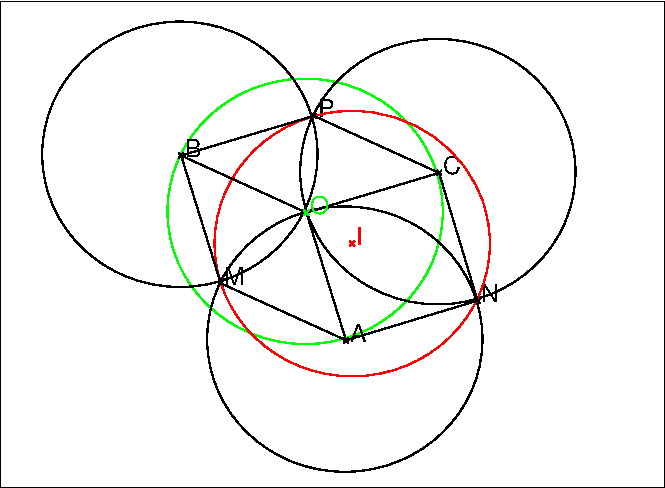
\includegraphics[width=\textwidth]{casjohn}\\

{\bf Lemme}\\
Si deux cercles de m\^eme rayon $R$ et de centre $O_1$ et $O_2$ se coupent en 
$A$ e $B$ alors le quadrilat\`ere $O_1,A,O_2,B$ est un losange.\\

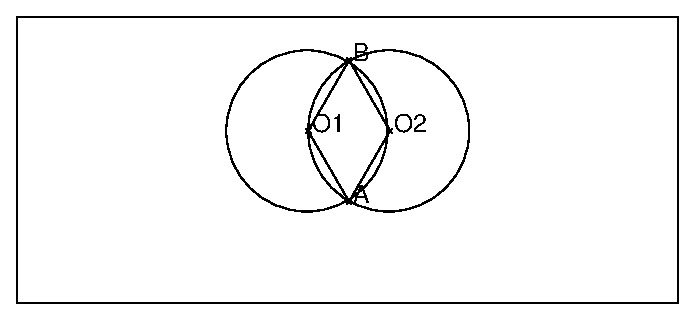
\includegraphics[width=\textwidth]{casjohn0}\\
En effet on a $O_1A=O_1B=O_2A=O_2B=R$.\\

{\bf D\'emonstration}\\
D'apr\`es le lemme les quadrilat\`eres :\\
$O,B,M,A$,\\
 $O,A,N,C$, et \\ 
$O,C,P,B$ \\
sont des losanges.\\ 
La translation de vecteur $\overrightarrow{OA}$ transforme  
$\overrightarrow{BC}$ en $\overrightarrow{MN}$.\\
La translation de vecteur $\overrightarrow{OB}$ transforme  
$\overrightarrow{AC}$ en $\overrightarrow{MP}$.\\
La translation de vecteur $\overrightarrow{OC}$ transforme  
$\overrightarrow{AB}$ en $\overrightarrow{NP}$.\\
Les triangles $M,N,P$ et $B,C,A$ sont donc \'egaux.\\
Donc le rayon $R$ du cercle circonscrit \`a  $B,C,A$ est \'egal au rayon du 
cercle circonscrit \`a  $M,N,P$.\\
On va aussi montrer que le centre $I$ de ce cercle est tel que 
$\overrightarrow{AI}= \overrightarrow{OP}$ et que \\
c'est aussi l'orthocentre du triangle $ABC$.\\
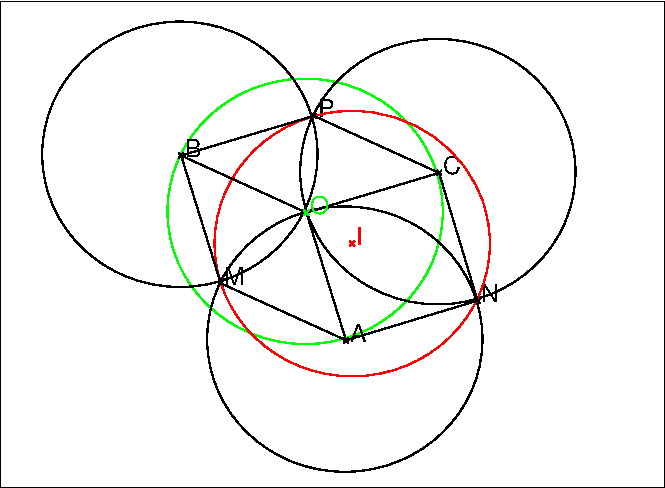
\includegraphics[width=\textwidth]{casjohn}
On a en effet :\\
Soit $\overrightarrow{AI}= \overrightarrow{OP}$\\
 On a $\overrightarrow{PI}= \overrightarrow{OA}= \overrightarrow{CN}$ et
$PC=CN$ donc \\
 $PINC$ est un losange et donc $IC$ est la m\'ediatrice de $PN$.\\
de m\^eme  $\overrightarrow{PI}= \overrightarrow{OA}= \overrightarrow{BM}$ et
$PB=BM$ donc \\
 $PIMB$ est un losange et donc $IB$ est la m\'ediatrice de $PM$.\\
Donc $I$ est le point de concours des m\'ediatrice de $MNP$ c'est donc le 
centre du cercle circonscrit \`a $MNP$.\\
Puisque $OP$ est la m\'ediatrice de $BC$ donc $AI$ est la m\'ediatrice de 
$MN$ (car la translation de vecteur $\overrightarrow{0A}$ transforme $B$ en $M$, $C$ en $N$ $P$ en $I$ et $O$ en $A$).\\
Donc la m\'ediatrice de $MN$ passe par $A$ puisque $MA=AN$ et elle est 
perpendiculaire \`a $BC$ puisque $BC$ et $MN$ sont parall\`eles. donc la 
m\'ediatrice de $MN$ est la hauteur issue de $A$ du triangle $ABC$.\\
De m\^eme la m\'ediatrice de $MP$ passe par $B$ puisque $MB=BP$ et elle est 
perpendiculaire \`a $AC$ puisque $AC$ et $MP$ sont parall\`eles. donc la 
m\'ediatrice de $MP$ est la hauteur issue de $B$ du triangle $ABC$.\\
donc le centre du cercle circonscrit \`a $MNP$ est l'orthocenntre du triangle 
$ABC$.\\

{\bf D\'emonstration avec {\tt Xcas}}\\
On tape :
\begin{verbatim}
O:=point(0);
U:=cercle(O,1):;U;
supposons(a=[0.3,-5,5,0.1]);
A:=point(cos(a)+(i)*sin(a));
supposons(b=[2.4,-5,5,0.1]);
B:=point(cos(b)+i*sin(b));
C1:=cercle(A,1):;C1;
C2:=cercle(B,1):;C2;
M:=normal(symetrie(droite(A,B),O));
supposons(c=[-1.6,-5,5,0.1]);
C:=point(cos(c)+(i)*sin(c));
C3:=cercle(C,1):;C3;
N:=normal(symetrie(droite(A,C),O));
P:=normal(symetrie(droite(B,C),O));
U1:=circonscrit(M,N,P):;
affichage(U1,1);
affichage(circonscrit(A,B,C),2);
I:=orthocentre(A,B,C);
U2:=cercle(I,1):; affichage(U2,4);
\end{verbatim}
{\tt Xcas}  peut prouver que le cercle {\tt U1} est le cercle  {\tt U2} de 
centre {\tt I} (orthocentre de {\tt ABC} ou point v\'erifiant 
$\overrightarrow{AI}= \overrightarrow{OP}$) et de rayon 1 car tous les calculs 
sont faits en utilisant les param\`etre formels {\tt a,b,c}.\\
On tape :\\
{\tt tsimplify(centre(U1)-I)}\\
On obtient :\\
{\tt 0}\\
On tape :\\
{\tt J:=translation(P-O,A)}\\
{\tt tsimplify(centre(U1)-J)}\\
On obtient :\\
{\tt 0}\\
On tape :\\
{\tt tsimplify(rayon(U1))}\\
On obtient :\\
{\tt 1}
{\bf Remarque}\\
On remarque que les calculs sont longs :\\
pour le cercle {\tt U1:=circonscrit(M,N,P):;} (Evaluation time: 2.74)\\
pour {\tt tsimplify(centre(U1)-I)} (Evaluation time: 0.54)\\
pour {\tt ttsimplify(rayon(U1))} (Evaluation time: 1.12)\\
On peut am\'lioer le temps de calcul !!!!
En effet lorsque vous voulez faire faire une d\'emonstration g\'eom\'etrique 
par {\tt Xcas}, il est important de r\'eduire au maximum les param\`etres 
formels sans perte de g\'en\'eralit\'es bien s\^ur !\\
Par exemple, ici, on peut supposer que {\tt a} vaut 1 et donc que {\tt A} se 
trouve sur {\tt U} et sur l'axe des $x$ (cette disposition n'est pas un cas 
particulier car on a le choix du rep\`ere). 
On tape :
\begin{verbatim}
O:=point(0);
U:=cercle(O,1):;U;
A:=point(1);
supposons(b=[2.4,-5,5,0.1]);
B:=point(cos(b)+i*sin(b));
C1:=cercle(A,1):;C1;
C2:=cercle(B,1):;C2;
M:=normal(symetrie(droite(A,B),O));
supposons(c=[-1.6,-5,5,0.1]);
C:=point(cos(c)+(i)*sin(c));
C3:=cercle(C,1):;C3;
N:=normal(symetrie(droite(A,C),O));
P:=normal(symetrie(droite(B,C),O));
U1:=circonscrit(M,N,P):;
affichage(U1,1);
affichage(circonscrit(A,B,C),2);
I:=orthocentre(A,B,C);
U2:=cercle(I,1):; affichage(U2,4);
\end{verbatim}
On a alors :\\
pour le cercle {\tt U1:=circonscrit(M,N,P):;} (Evaluation time: 0.92)\\
et ensuite {\tt tsimplify(centre(U1)-I)} et  {\tt ttsimplify(rayon(U1))} sont
instantan\'es.

\section{Une suite de sym\'etrie}
On se donne trois directions $d_1,d_2,d_3$ et un cercle $C$ de centre $O$ et de 
rayon $R$ et un point $M_0$ sur ce cercle.\\
On consid`ere la suite des points :
$M_1$ est le point de $C$ tel que $M_0M_1$ a pour direction $d_1$,\\
$M_2$ est le point de $C$ tel que $M_1M_2$ a pour direction $d_2$,\\
$M_3$ est le point de $C$ tel que $M_2M_3$ a pour direction $d_3$,\\
$M_4$ est le point de $C$ tel que $M_3M_4$ a pour direction $d_1$,\\
$M_5$ est le point de $C$ tel que $M_4M_5$ a pour direction $d_2$,\\
$M_6$ est le point de $C$ tel que $M_5M_6$ a pour direction $d_3$,\\
Montrer que $M_6=M_0$.\\
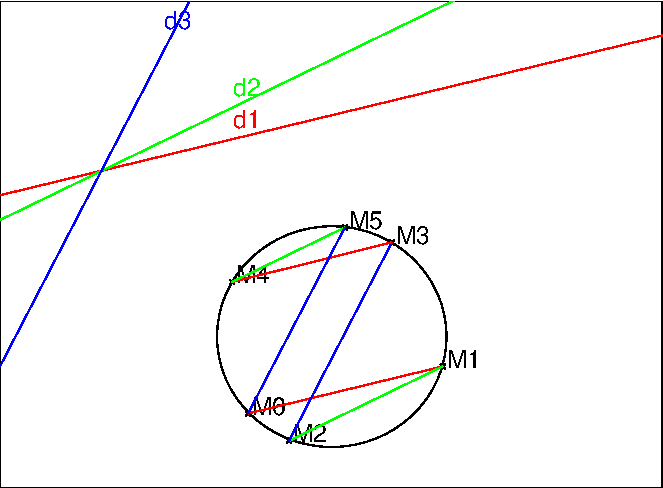
\includegraphics[width=\textwidth]{cassym}\\
{\bf D\'emonstration}\\
Soient $\Delta_1,\Delta_2,\Delta_3$ 3 droites passant par $O$ et ayant comme 
directions, les directions perpendiculaires \`a 
$d_1,d_2,d_3$. Soient $S-1,S_2,S_3$ les 3 sym\'etries droites d'axe 
$\Delta_1,\Delta_2,\Delta_3$.\\
On a :\\
$M_1=S_1(M_0)$,\\
$M_2=S_2(M_1)$,\\
$M_3=S_3(M_2)$,\\
$M_4=S_1(M_3)$,\\
$M_5=S_2(M_4)$,\\
$M_6=S_3(M_5)=S_3\circ S_2\circ S_1\circ S_3\circ S_2\circ S_1(M_0)$\\
on sait que :\\
le produit des 2 sym\'etries $S_2\circ S_1$ est une rotation de 
centre $0$ et d'angle $2(\Delta_1,\Delta_2)$.\\
le produit des 2 sym\'etries $S_1\circ S_3$ est une rotation de 
centre $0$ et d'angle $2(\Delta_3,\Delta_1)$.\\
le produit des 2 sym\'etries $S_3\circ S_2$ est une rotation de 
centre $0$ et d'angle $2(\Delta_2,\Delta_3)$.\\
Donc $S_3\circ S_2\circ S_1\circ S_3\circ S_2\circ S_1$ est une rotation de centre $O$ et d'angle :\\
$2(\Delta_1,\Delta_2)+2(\Delta_3,\Delta_1)+2(\Delta_2,\Delta_3)=0 \bmod 2\pi$.\\
Donc  $S_3\circ S_2\circ S_1\circ S_3\circ S_2\circ S_1$ est l'identit\'e.\\

{\bf D\'emonstration avec {\tt Xcas}}\\
On tape :
\begin{verbatim}
supposons(a=[0.6,-5,5,0.1]);
supposons(b=[1.2,-5,5,0.1]);
supposons(c=[2.0,-5,5,0.1]);
d1:=droite(y=2+a*(x+2), affichage=1);
d2:=droite(y=2+b*(x+2), affichage=2);
d3:=droite(y=2+c*(x+2), affichage=4);
C:=cercle(0,1):;C;
supposons(d=[0.6,-5,5,0.1]);
M0:=point(exp((i)*d));
M1:=symetrie(droite(y=-x/a), M0);
M2:=symetrie(droite(y=-x/b), M1);
M3:=symetrie(droite(y=-x/c), M2);
M4:=symetrie(droite(y=-x/a), M3);
M5:=symetrie(droite(y=-x/b), M4);
M6:=symetrie(droite(y=-x/c), M5);
segment(M0,M1,affichage=1);
segment(M2,M1,affichage=2);
segment(M2,M3,affichage=4);
segment(M3,M4,affichage=1);
segment(M4,M5,affichage=2);
segment(M5,M6,affichage=4);
\end{verbatim}
On obtient :\\
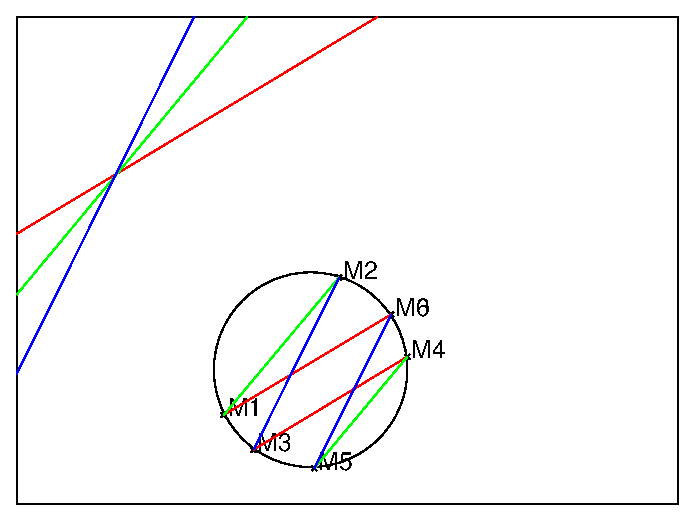
\includegraphics[width=\textwidth]{cassymd}
On tape :\\
{\tt affixe(M0)==normal(affixe(M6))}\\
On obtient :\\
{\tt 1}

\section{Une suite de projections}
On consid\`ere un triangle \'equilat\`eral $ABC$ et un point $M_1$ sur $AB$.\\
$M_1$ se projette orthogonalement en $H_1$ sur $BC$,\\
$H_1$ se projette orthogonalement en $K_1$ sur $AC$ et\\
$K_1$ se projette orthogonalement en $M_2$ sur $AB$ etc....\\
On obtient ainsi sur $AB$ une suite de points $M_n$.\\
On pose $AM_n=x_nAB$.\\
Calculer $x_n$ et \'etudier la suite $x$.\\
On commence par faire la figure.\\
 On \'ecrit pour cela la suite d'instructions dans un niveau de g\'eom\'etrie :
\begin{verbatim}
A:=point(0);
B:=point(1);
C:=point(1/2+sqrt(3)*i/2);
triangle(A,B,C);
assume(a=[0.1,0,1]);
M:=element(segment(A,B),a);
L:=[normal(affixe(M))];
for (k:=1;k<=30;k:=k+3) {
L:=append(L,normal(affixe(projection(segment(B,C),L[k-1]))));
L:=append(L,normal(affixe(projection(segment(A,C),L[k]))));
L:=append(L,normal(affixe(projection(segment(B,A),L[k+1]))));
};
polygone_ouvert(L);
\end{verbatim} 
On obtient la figure dans l'\'ecran de g\'eom\'etrie.\\
 On rappelle que :\\
{\tt M:=element(segment(A,B),a)} signifie que :\\
$\overline{AM}=a\overline{AB}$ et $0 \leq b \leq 1$.
On rappelle aussi que :\\
{\tt assume(a=[0.1,0,1])} signifie que :\\
la figure se fera avec {\tt a=0.1} mais que les calculs se feront avec le 
param\`etre formel {\tt a} compris entre 0 et 1.
On r\'egle la fen\^etre graphique :\\
{\tt xyztrange(-0.1,2.0,-0.1,1.0,-10.0,10.0,-1.0,6.0,-0.1,2.0,\\
-0.146865136298,1.0,1,0.0,1.0) }\\
On tape L dans une entr\'ee de commande et on pbtient :\\
{\tt [a,((-i)*sqrt(3)+1)/4*a+((i)*sqrt(3)+3)/4,\\
((-i)*sqrt(3)-1)/8*a+((3*i)*sqrt(3)+3)/8,-a/8+3/8,....]}\\
ce qui signifie que :\\
${\tt x_1=a}$ et ${\tt x_2=-a/8+3/8}$\\
Pour avoir la suite $x_n$ on tape :\\
{\tt Xn:=seq(L[k],k,0,30,3)}
On trouve : $x_{11}=a/1073741824+357913941/1073741824$\\
On tape :\\
{\tt evalf(357913941/1073741824)}\\
On obtient:\\
{\tt 0.333333333023}\\
Il semble donc que cette suite converge vers $N$ tel que $AN=AB/3$.
\subsection{La d\'emonstration}
On calcule $x_2$ en fonction de $x_1$ :
on a $AM_1=x_1AB$\\
$BH_1=(1-x_1)/2BC$ et $CK_1=(1-(1-x_1)/2)/2CA=(1+x_1)/4CA$\\
$AM_2=(1-(1+x_1)/4)/2AB=(3-x_1)/8AB$\\
La relation de r\'ecurrence est :\\
$x_{n+1}=(3-x_n)/8$
On cherche la limite $l$ possible :\\
$l=(3-l)/8$ donc $8l=3-l$ soit $l=3/9=1/3$\\
La suite $u_n=x_n-1/3$ est une suite g\'eom\'etrique de raison $-1/8$
puisque $u_{n+1}=x_{n+1}-1/3=(3-x_n)/8-(3-l)/8=-u_n/8$.\\
La suite $u_n=x_n-1/3$ converge vers 0 donc la suite $x_n$ converge vers $1/3$
\section{Un tableau fait avec des sinusoides}
On veut dessiner sur un m\^eme graphique la fonction d\'erivable qui vaut pour
$a<b<c<d$ :
$\sin(x)$ sur $[a,b]$,$\sin(2*x+\alpha)$ sur $[b,c]$ et $\sin(x)$t sur $[c,d]$ 
en raccordant les graphes de $\sin(x)$ et de $\sin(2*x+\alpha)$ en des
 points o\`u ils ont une m\^eme tangente horizontale. Il faut donc choisir 
correctement $b,c,\alpha$.\\
On tape par exemple :
\begin{verbatim}
sinusoide0():={
  local L1,L2,L3,R,k;
  L1:=plotfunc(sin(x),x=-9*pi/2..-pi/2,affichage=epaisseur_ligne_3);
  L2:=plotfunc(sin(2*x+pi/2),x=-pi/2..3*pi/2,affichage=epaisseur_ligne_3);
  L3:=plotfunc(sin(x),x=3*pi/2..9*pi/2,affichage=epaisseur_ligne_3);
  R:=L1,L2,L3;
  retourne R;
}:;
\end{verbatim}
On tape : {\tt sinusoide0()}\\
On obtient :\\
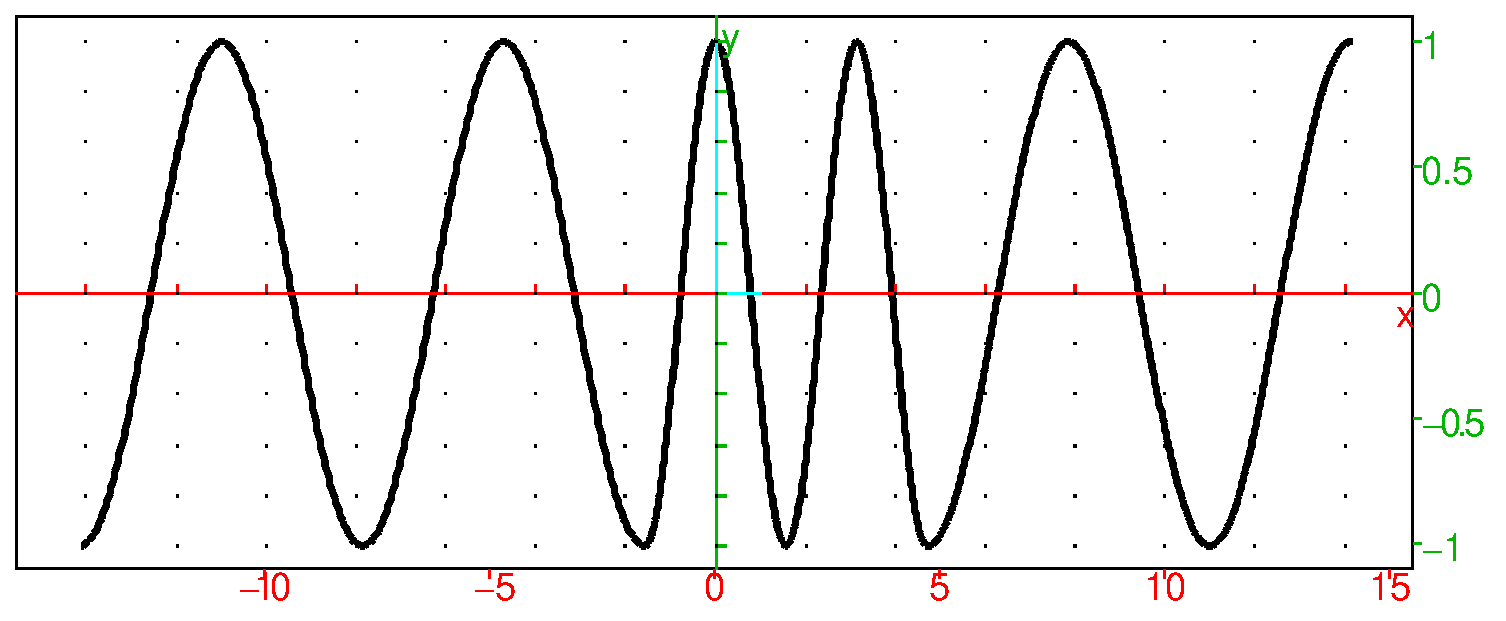
\includegraphics[width=\textwidth]{sinusoide0}
On veut tracer des translat\'es de ces graphes selon des vecteurs de direction
$Oy$. \\
On tape par exemple pour effectuer 7 translations sur la premi\`ere sinusoide :
\begin{verbatim}
sinusoide1():={
  local L,R,k;
  L:=plotfunc(sin(x),x=-9*pi/2..-pi/2,affichage=epaisseur_ligne_3);
  R:=(L+k*i)$(k=-3..3);
  retourne R;
}:;
\end{verbatim}
On tape : {\tt sinusoide1()}\\
On obtient :\\
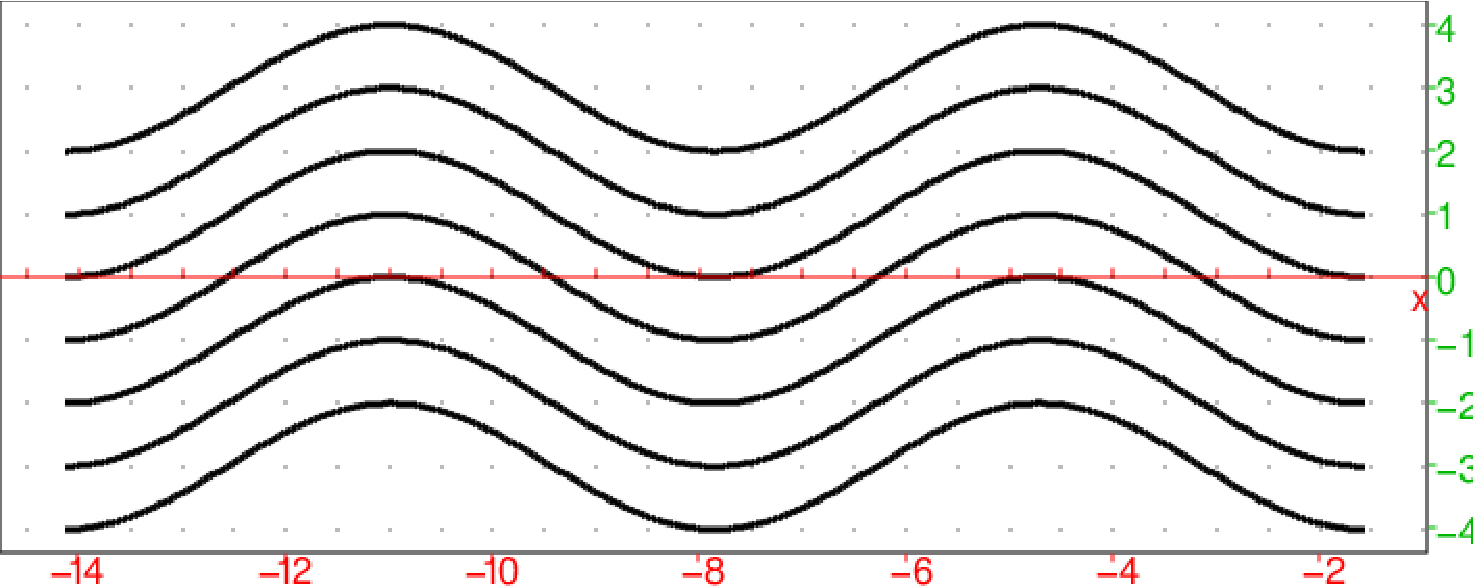
\includegraphics[width=\textwidth]{sinusoide1}
On tape par exemple pour effectuer 46 translations sur les 3 sinusoides:
\begin{verbatim}
sinusoide():={
  local L1,L2,L3,R,k;
  L1:=plotfunc(sin(x),x=-9*pi/2..-pi/2,affichage=epaisseur_ligne_3);
  L2:=plotfunc(sin(2*x+pi/2),x=-pi/2..3*pi/2,affichage=epaisseur_ligne_3);
  L3:=plotfunc(sin(x),x=3*pi/2..9*pi/2,affichage=epaisseur_ligne_3);
  R:=(L1+k/4*i)$(k=-20..25),(L2+k/4*i)$(k=-20..25),(L3+k/4*i)$(k=-20..25);
  retourne R;
}:;
\end{verbatim}
On tape : {\tt sinusoide()}\\
On obtient une sinusoide.

\section{La suite de Syracuse}
Soit $a$ un entier positif. On veut \'etudier avec des graphiques la suite de 
Syracuse d\'efinie par :\\
$u_0=a$\\
$u_n=u_{n-1}/2$ si $u_{n-1}$ est pair et\\
$u_n=3*u_{n-1}+1$ si $u_{n-1}$ est impair.\\
Cette suite se termine toujours (?) par 1,4,2,1,4,2,1... mais on ne sait pas 
le montrer.\\
Pour \'etudier cette suite on peut :\\
- utiliser le tableur en mettant dans {\tt A0} la valeur $a$ de d\'epart et 
dans {\tt A1} la formule :\\
{\tt =ifte(irem(A0,2)==0,iquo(A0,2),3*A0+1)} ou encore \\
{\tt =if ((irem(A0,2))==0) iquo(A0,2); else 1+3*A0;}\\
- utiliser un programme {\tt syracuse} qui renvoie le maximum de cette suite et
 le nombre d'\'el\'ements de cette suite et  {\tt syracuse0} qui \'ecrit en 
plus les termes de la suite ou encore {\tt syracuse100}
qui renvoie le maximum, le nombre de termes et la valeur de d\'epart de la 
plus longue suite d\'emarrant par un nombre entre 2 et 100.
\begin{verbatim}
  syracuse(a):={
    local k,m;
    k:=0;
    m:=a;
    while (a!=1) {
      if (irem(a,2)==0) a:=iquo(a,2); 
      else {
	a:=a*3+1;
	if (a>m){m:=a};
      }
      k:=k+1;
    }
  retourne m,k;
}:;
  
 syracuse0(a):={
    local m,k;
    m:=a;
    k:=0;
    print(a);
    while (irem(a,2)==0){
      a:=iquo(a,2);
      k:=k+1;
      print(a);
    }
    while(a!=1){
      a:=3*a+1;
      k:=k+1;
      print(a);
      if (m<a) {m:=a;}
      while (irem(a,2)==0){
	a:=iquo(a,2);
	k:=k+1;
    print(a);
      }
    }
    return(m,k);
  };
  
  syracuse100():={
    local k,kn,kt,l,lt,m,mt;
    lt:=0;
    for (k:=2;k<101;k:=k+1){
      kn:=k;
      m:=k;
      l:=0;
      while (kn!=1) {
	if (irem(kn,2)==0) kn:=iquo(kn,2); 
	else {
	  kn:=kn*3+1;
	  if (m<kn) {
	    m:=kn;
	  }
	}
	l:=l+1;
      }
      if (l>lt) {
	mt:=m;lt:=l;kt:=k;
      }
    }
    return(mt,lt,kt);
  };
\end{verbatim}
On ouvre un \'editeur de programme, on recopie la proc\'edure, puis gr\^ace au 
bouton {\tt OK} le programme est valid\'e.\\
On tape {\tt syracuse100()}, on trouve :\\
{\tt 9232,118,97} ce qui veut dire que c'est en d\'emarrant avec 97 que la 
suite a le plus de termes (ici 118 termes) et le maximum de cette suite est 
9232. \\
On peut bien s\^ur modifier les param\`etres de la boucle {\tt for} en mettant 
par exemple :\\
{\tt for (k:=101;k<200;k:=k+1)}\\
On tape {\tt syracuse100()}, on trouve alors :\\
{\tt 250504,124,177}\\
ou encore :\\
{\tt for (k:=901;k<1000;k:=k+1)}\\
On tape {\tt syracuse100()}, on trouve alors :\\
{\tt 250504,173,937}\\
On peut encore modifier facilement pour savoir si un plus grand nombre de 
terme donne la plus grande valeur atteinte (cela semble vrai!!!) en changeant 
pour cela :\\
{\tt if (l>lt) \{mt:=m;lt:=l;kt:=k;\}} en \\
{\tt if (m>mt) \{mt:=m;lt:=l;kt:=k;\}} et rajouter au d\'ebut  {\tt kt:=2;}.\\
- utiliser un programme qui dessine les points $(n,u_n)$ lorsqu'on donne en 
entr\'ee $u_0=a$\\
- lorsqu'on donne en entr\'ee $u_0=a$ et en notant $n$ la premi\`ere valeur de 
$k$ pour laquelle $u_k=1$ et $m$ le maximum des $u_k$ pour $k\leq n$, dessiner 
les points $a,m$ ou encore dessiner les points  $a,u_k$ pour $k=0..n$.\\
On \'ecrit la proc\'edure {\tt syracuse1} (resp {\tt syracuse2}) qui dessine 
 les points $(k,u_k)$ (resp les segments reliant les points $(k,u_k)$) dans 
l'\'ecran de g\'eom\'etrie et la proc\'edure {\tt syracuse3} qui
 dessine les points $a,u_k$ pour $k$ allant de 0  \`a $n$ et cela pour $a$ 
allant de 2 \`a 100 :
\begin{verbatim}
  syracuse1(a):={
    local m,k;
    m:=a;
    k:=0;
    point(0,a);
    while (irem(a,2)==0){
      a:=iquo(a,2);
      k:=k+1;
      point(k,a);
    }
    while(a!=1){
      a:=3*a+1;
      k:=k+1;
      point(k,a);
      if (m<a) {m:=a;}
      while (irem(a,2)==0){
	a:=iquo(a,2);
	k:=k+1;
	point(k,a);
      }
    }
    return(m,k);
  };
  
  
  syracuse2(a):={
    local m,k,k0,a0;
    m:=a;
    k:=0;
    point(k,a);
    while (irem(a,2)==0){
      k0:=k;
      a0:=a;
      a:=iquo(a,2); 
      k:=k+1;
      segment(k0+i*a0,k+i*a);
    }
    while(a!=1){
      k0:=k;
      a0:=a;
      a:=3*a+1;
      k:=k+1;
      segment(k0+i*a0,k+i*a);
      if (m<a) {m:=a;}
      while (irem(a,2)==0){
	k0:=k;
	a0:=a;
	a:=iquo(a,2);
	k:=k+1;
	segment(k0+i*a0,k+i*a);
      }
    }
    return(m,k);
  };
  
  syracuse3():={
    local k,kn;
    for(k:=2;k<101;k:=k+1){
      point(k,k);
      kn:=k;
      while (kn!=1) {
	if (irem(kn,2)==0) kn:=iquo(kn,2); else kn:=kn*3+1;
	point(k,kn);
      }
    }
  };
\end{verbatim}
Ne pas oubler de r\'egler la fen\^etre graphique en mettant par exemple :
{\tt X-=Y-=WX-=WY-=0}, {\tt X+=WX+=100} et {\tt Y+=WY+=1000}.\\
puis on tape par exemple {\tt syracuse1(123)}.

\section{La suite des tas}
On dispose $k$ jetons en $p$ tas.\\
On construit la suite des tas de la fa\c{c}on suivante :\\
on prend un jeton dans chaque tas et tous ces jetons forment un nouveau tas qui
sera le dernier tas, et on recommence.\\
Ce qui est s\^ur c'est que cette suite de tas est p\'erodique puisque il n'y a
qu'un nombre fini de fa\c{c}ons de disposer $k$ jetons en tas.\\
Il s'agit de voir comment se comporte cette suite.\\
On peut montre que lorsque $k=n*(n+1)/2$ cette suite stationne en :\\
$1,2,3,...,n$.\\
\subsection{Une remarque}
{\bf Lemme} La suite d\'ebutant par $1,2,3,...,n$ non ordonn\`e stationne 
vers $1,2,3,...,n$.\\
En effet, si on r\'epartit les jetons en $n$ tas $1,2,3,...,n$ de fa\c{c}on
non  ordonn\'ee, on 
aura la suite ordonn\'ee $1,2,3,...,n$ au bout d'au plus $n-1$ manipulations.\\
En effet \`a la premi\`ere \'etape $n$ se trouvera en dernier, \`a la 
deuxi\`eme \'etape $n-1,n$ se trouveront \`a la fin, et  \`a la $(n-1)$-i\`eme
 \'etape $2, ...n-1,n$ se trouvera en dernier et on aura donc obtenu $1,2...n$
puisque le nombre $k$ de jetons vaut $n(n-1)/2$.\\
\subsection{Le programme de simulation}
\begin{verbatim}
//programme de simulation tas.cxx
tas(l):={
local s,j,k,lr;
lr:=[l];
while (1) {
s:=size(l);
for (j:=0;j<s;j++) {
l[j]:=l[j]-1;
}
l:=concat(l,s);
//on supprime les zeros de l
k:=0;
for (j:=0;j<s+1;j++){
if (l[j]!=0){
l[k]:=l[j];
k:=k+1;
}
}
l:=mid(l,0,k);
if (member(l,lr)) return lr;
lr:=append(lr,l);
}
}

\end{verbatim}
On tape :\\
{\tt tas([10])}\\
On obtient :\\
{\tt [[10],[9,1],[8,2],[7,1,2],[6,1,3],[5,2,3],} \\
{\tt [4,1,2,3],[3,1,2,4],[2,1,3,4],[1,2,3,4]]}
\chapter{Pour s'amuser avec les mesures}
\section{La ficelle et la terre}
Imaginez qu'avec une ficelle vous fassiez le tour de la terre. Puis vous 
rajoutez un m\`etre \`a cette ficelle et vous ceinturez \`a nouveau la terre. 
\`A quelle distance du sol va alors se trouver la ficelle ?\\
M\^eme question avec une balle de tennis.\\

Si $r$ est le rayon de la terre en m\`etre (ou de la balle de tennis), son 
p\'erim\`etre est donc : $2\pi r$. La ficelle va donc mesurer $2\pi r+1$ et 
cela correspond \`a un rayon $R$ v\'erifiant $2\pi r+1=2\pi R$.
Donc $2\pi (R-r)=1$ c'est \`a dire $R-r=1/(2\pi)$.\\
On tape :\\
{\tt evalf(1/2/pi)}\\
On obtient :\\
{\tt 0.159154943092}\\
Donc quelque soit le rayon de la sph\`ere la ficelle va \^etre \`a environ 
15.9 cm de la surface de la sph\`ere.
\section{Les lunules d'Hippocrate}
Ce th\'eorème, très ancien, a \'et\'e d\'emontr\'e par Hippocrate de Chios 
(-500) (Ne pas le confondre avec Hippocrate de Cos, le m\'edecin), qui \'etudia 
aussi la duplication du cube, c’est-à-dire le calcul de la racine cubique de 2.\\
Hippocrate recherchait alors la quadrature du cercle et pensait que la 
quadrature de ses lunules allait le rapprocher du but.\\
Une lunule est une portion de surface d\'elimit\'ee par deux arcs de cercles 
non concentriques de rayons diff\'erents. Ces arcs ont m\^emes extr\'emit\'es et
forment un croissant de lune en forme de m\'enisque : convexe d’un côt\'e et 
concave de l’autre.\\
{\bf Construction}\\
Soit le triangle $ABC$ rectangle en $A$ et $\mathcal{C}$ le cercle circonscrit 
à $ABC$ (de diamètre $BC$).\\
La lunule $L_{AC}$ est la figure form\'ee par le demi-disque de diamètre $AC$ 
ext\'erieur au triangle $ABC$, auquel on enlève son intersection avec le disque 
d\'elimit\'e par $\mathcal{C}$.\\
La lunule $L_{AB}$ est la figure form\'ee par le demi-disque de diamètre $AB$ 
ext\'erieur au triangle $ABC$, auquel on enlève son intersection avec le disque 
d\'elimit\'e par $\mathcal{C}$.
Ces deux lunules sont appel\'ees {\bf lunules d'Hippocrate}.
Alors la somme des aires de $L_{BC}$ et de $L_{BA}$ (en jaune) est \'egale à 
l'aire du triangle $ABC$ (en rouge).
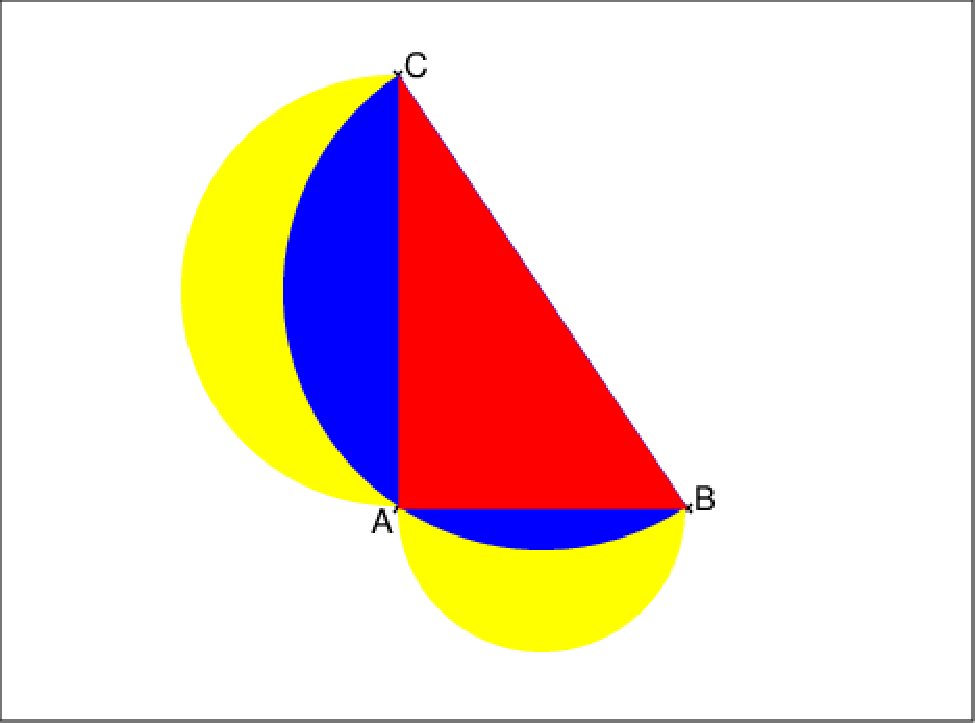
\includegraphics[width=\textwidth]{lunules}
On calcule $S1$ l'aire du triangle $ABC$ :\\
$S1=AB*AC/2$
On calcule $S2$ la somme des aires de $L_{BC}$ et de $L_{BA}$ :\\
$S2$ est obtenue par diff\'erence : $S2$ est \'egale \`a la somme des aires des
demi-cercles de diam\`etres $AB$ et $AC$ \`a laquelle on enl\`eve l'aire en 
bleu.\\
L'aire en bleu est \'egale \`a l'aire du demi-cercle de 
diam\`etre $BC$ \`a laquelle on enl\`eve l'aire $S1$ du triangle $ABC$ :\\
$S2=\pi*AB^2/2+\pi*AC^2/2-(\pi*BC^2/2-S1)$\\
D'apr\`es le th\'eor\`eme de Pythagore on a  : $AB^2+AC^2=BC^2$ donc :\\
$S2=S1$.\\
Pour faire la figure on a tap\'e :
\begin{verbatim}
A:=point(0);
B:=point(2,affichage=quadrant1);
C:=point(3*i,affichage=quadrant1);
cercle(A,C,0,pi,affichage=3+rempli);
cercle(A,B,-pi,0,affichage=3+rempli);
cercle(B,C,0,pi,affichage=4+rempli);
triangle(A,B,C,affichage=1+rempli);
\end{verbatim}
{\tt Xcas} sait remplir de couleur les polygones et les secteurs circulaires.
On est donc oblig\'e de proc\'eder par superposition de couleur pour remplir 
les lunules d'Hippocrate et cela symbolise les op\'erations que l'on fait pour 
calculer l'aire des 2 lunules.\\
{\bf Exercice}\\
Soient un carr\'e de c\^ot\'es $l$ et les cercles ayant comme 
diam\`etre les c\^ot\'es du carr\'e.\\
\`A l'ext\'erieur du carr\'e, ces cercles d\'eterminent avec le cercle 
circonscrit au carr\'e 4 lunules.\\
Trouver l'aire des 4 lunules ainsi d\'etermin\'ees.\\
\`A l'int\'erieur du carr\'e, ces cercles en se coupant d\'eterminent 4 
"p\'etales".\\
 Trouver l'aire des 4 "p\'etales" ainsi d\'etermin\'ees.\\
{\bf La solution}
Un carr\'e est form\'e de 2 triangles rectangles donc l'aire des 4 lunules est 
\'egale \`a l'aire du carr\'e.\\
La somme de l''aire du carr\'e et de  l'aire des "p\'etales" est \'egale \`a 
l'aire des 4 demi-cercles de rayon $l/2$ donc 
l'aire des "p\'etales"=$\pi*l^2/2-l^2$
\section{Aire d'un cercle trou\'e}
On perce un cercle de rayon $R$ avec un cercle de m\^eme centre et de rayon $r$. Quelle est l'aire de ce cercle trou\'e. Exprimer cette aire en fonction de  
$d=\sqrt{R^2-r^2}$.\\
On sait que l'aire d'un cercle de rayon $R$ est : $\pi R^2$
L'aire du cercle trou\'e est donc :
$$\pi(R^2-r^2)=\pi d^2$$
L'aire d'un cercle trou\'e est \'egale \`a l'aire du cercle de rayon $d$ o\`u 
$d$ est la longueur de la demi-corde qui est tangente au trou.
\section{Volume de la sph\`ere trou\'ee}
\subsection{Volume de la calotte de hauteur $h$ d'une sph\`ere de rayon $R$}
On note $R$ le rayon de la sp\`ere, $r$ le rayon de la base de la calotte et 
$h$ la hauteur de la calotte et on suppose que $0<h<R$. 0n a donc :
$r^2=R^2-(R-h)^2$\\
On tape :\\
{\tt assume(R>0 and h>0 and h<R)}\\
On calcule une int\'egrale triple :\\
$\int_0^{2*\pi}(\int_0^r(\int_0^{\sqrt{R^2-r^2}}dz)*\rho d\rho)d\theta$\\
On tape :
\begin{center}{\tt factor(int(int(int(1,z,R-h,sqrt(R\verb|^|2-ro\verb|^|2))*ro,\\
                ro,0,sqrt(R\verb|^|2-(R-h)\verb|^|2)),t,0,2*pi))}\end{center}
On obtient :\\
{\tt (h\verb|^|2*pi*(3*R-h))/3}\\
Donc le volume de la calotte de hauteur $h$ d'une sp\`ere de rayon $R$ est :
$$V_C=\pi h^2\frac{3*R-h}{3}$$
{\bf V\'erification}
On sait que le volume d'une sph\`ere de rayon $R$ est : $\frac{4}{3}\pi R^3$
Le volume de 2 calottes sph\'eriques de rayon $R$ a pour hauteur $R$ est :\\
 $2\pi R^2\frac{3*R-R}{3}=\frac{4}{3}\pi R^3$
\subsection{Volume d'une sph\`ere trou\'ee}
On perce une sph\`ere de rayon $R$ avec un cylindre ayant pour axe un 
diam\`etre de la sph\`ere et comme base un cercle de rayon $r$. Quelle est le 
volume de cette sph\`ere trou\`ee. Exprimer ce volume  en fonction de  
$d=\sqrt{R^2-r^2}$.\\

Avec les notations pr\'ec\'edentes on a enlev\'e \`a la sph\`ere :\\
un cylindre ayant comme base un cercle de rayon $r$  comme hauteur $2d$ et 
comme volume $2\pi r^2d=2\pi (R^2-d^2)d$ et,\\
 2 calottes sph\'eriques ayant comme base 
un cercle de rayon $r$ et ayant comme hauteur $h=R-d$.\\
On sait que le volume d'une sph\`ere de rayon $R$ est : $\frac{4}{3}\pi R^3$
Le volume de cette sph\`ere trou\`ee est donc :\\
$$\frac{4}{3}\pi R^3-2\pi h^2\frac{3*R-h}{3}-2\pi r^2d$$
On tape :\\
{\tt factor(2*pi/3*(2*R\verb|^|3-(R-d)\verb|^|2*(3*R-(R-d))-3*(R\verb|^|2-d\verb|^|2)*d))}\\
On obtient :\\
{\tt (4*d\verb|^|3*pi)/3}\\
Donc le volume d'une sp\`ere de rayon $R$ trou\'ee par un cylindre d'axe un 
diam\`etre et de hauteur $2d$ est :
$$V_{ST}=\frac{4}{3}\pi d^3$$
c'est \`a dire le volume d'une sp\`ere de rayon $R$ trou\'ee par un cylindre d'axe un 
diam\`etre et de hauteur $2d$ est \'egal au volume d'une sph\`ere de rayon $d$.
\section{Puzzle transformant un rectangle 5x1 en un carr\'e}
On tape :
\begin{verbatim}
rectangle(-5,0,1/5):;
carre(-5,-4,affichage=1+rempli);
triangle(-4,-2,-2+i,affichage=2+rempli);
triangle(-4,-2+i,-4+i,affichage=3+rempli);
triangle(-2,0,-2+i,affichage=4+rempli);
triangle(0,i,-2+i,affichage=5+rempli);
carre(-3-5/2*i,-2-5/2*i, affichage=1+rempli));
triangle(-4-3/2*i,-2-3/2*i,-2-i/2,affichage=2+rempli);
triangle(-4-3/2*i,-3-3/2*i,-3-7/2*i,affichage=3+rempli);
triangle(-1-5/2*i,-3-5/2*i,-3-7/2*i,affichage=4+rempli);
triangle(-1-5/2*i,-2-5/2*i,-2-i/2,affichage=5+rempli);
\end{verbatim}
On obtient les 5 pi\`eces du puzzle du rectangle $5*1$ :\\
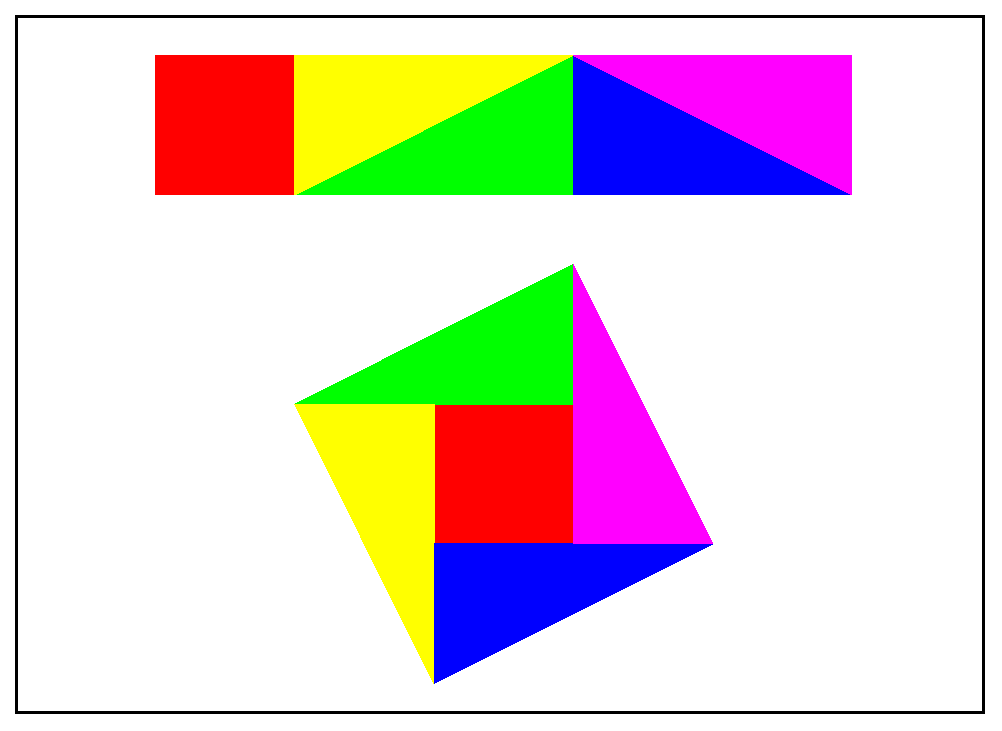
\includegraphics[width=\textwidth]{carresqrt5}
\section{Puzzle transformant un rectangle 3x2 en un carr\'e}
Soit un rectangle de longueur 3 unit\'es et de largeur 2 unit\'es.\\
On veut le partager en plusieurs morceaux pour pouvoir constituer avec 
tous ces morceaux un carr\'e.\\
On prend exemple sur le d\'ecoupage pr\'ec\'edent.\\
Le carr\'e doit avoir comme c\^ot\'e $\sqrt 6$ unit\'es.\\
$\sqrt 6$ est l'hypot\'enuse d'un triangle rectangle de c\^ot\'e 2 et 
$\sqrt 2$ (puisque $6=4+2=2^2+(\sqrt 2)^2=(\sqrt 6)^2$.\\
On utilise la formule :\\
$4*\sqrt 2+(2-\sqrt 2)^2=6$ et\\
On consid\`ere la droite $D$ d'\'equation $y=-\sqrt 2x+2$ (c'est la droite
portant l'hypot\'enuse du triangle $0,\sqrt 2,2$.\\
Puisque le point de coordonn\'ees $(1,2-\sqrt 2)$ est sur la droite $D$, on 
peut d\'ecouper le rectangle selon les 5 morceaux ci-dessous.\\
Voici ce puzzle fait avec ces 5 morceaux mais on remarquera qu'il suffit de 
d\'ecouper le rectangle en seulement 3 morceaux !!!\\
On tape :
\begin{verbatim}
rectangle(0,3,2/3):;
T1:=triangle(0,sqrt(2),2i):; affichage(T1,1+rempli);
T2:=triangle(1+2*i,1+(2-sqrt(2))*i,3+2*i):; 
affichage(T2,2+rempli);
T3:=triangle(3+2*i,1+(2-sqrt(2))*i,3+(2-sqrt(2))*i):; 
affichage(T3,3+rempli);
T4:=triangle(2i,1+(2-sqrt(2))*i,1+2i):; 
affichage(T4,4+rempli);
T5:=polygone(1+(2-sqrt(2))*i,sqrt(2),1+sqrt(2),1+sqrt(2)+(2-sqrt(2))*i):; 
affichage(T5,5+rempli);
T6:=carre(1+sqrt(2),3):;
affichage(T6,6+rempli);
carre(sqrt(2)-2,2i-2):;
affichage(translation(-2,T1),1+rempli);
affichage(translation(-5,T3),3+rempli);
affichage(translation(-5,T5),5+rempli);
affichage(translation(-5,T6),6+rempli);
affichage(translation(-3+sqrt(2)-2-2i,T2),2+rempli);
affichage(translation(-3+sqrt(2)-2-2i,T4),4+rempli);
\end{verbatim}
On obtient les 5 pi\`eces du puzzle du rectangle $3*2$ :\\
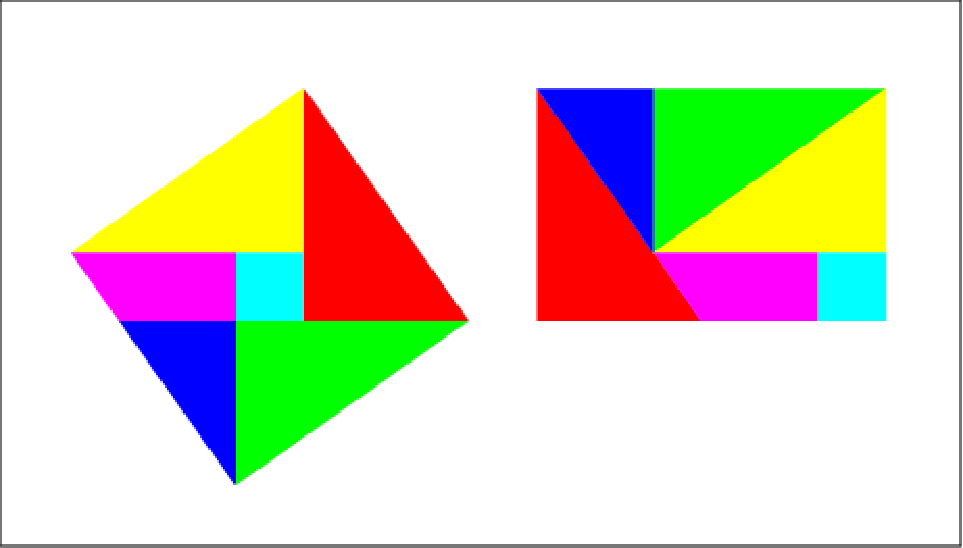
\includegraphics[width=\textwidth]{carresqrt6}
On obtient avec 3 pi\`eces :\\
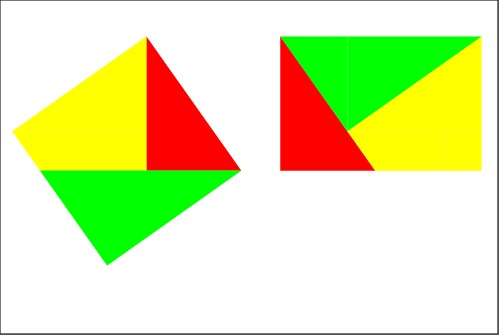
\includegraphics[width=\textwidth]{carresqrt63}
{\bf Autre solution}
Soit un rectangle de longueur 3 unit\'es et de largeur 2 unit\'es.\\
On veut le partager en plusieurs morceaux pour pouvoir constituer avec 
tous ces morceaux un carr\'e.\\
Il reste ensuite \`a d\'ecouper le rectangle $(3-\sqrt 5)*2$ en 3 morceaux pour
en faire un carr\'e selon la m\'ethode de la section \ref{sec:carreab}.\\
rappelons ce d\'ecoupage sur cet exemple.\\
On tape :
\begin{verbatim}
b:=3;a:=2;
A:=point(0);
B:=point(b);
C:=point(b+i*a);
D:=point(i*a);
rectangle(A,B,C,D);
P:=point(sqrt(a*b));
M:=point(b-sqrt(a*b)+i*a);
Q:=point(sqrt(a*b)*(1+i));
R:=point(sqrt(a*b)*i);
S:=point(sqrt(a*b)+i*a);
T:=point(sqrt(a*b)+i*(sqrt(a*b)-a));
carre(A,P,Q,R, affichage=rouge);
segment(P,D);
segment(B,M);
segment(R,M,affichage=bleu);
segment(P,S, affichage=vert);
\end{verbatim}
On obtient :\\
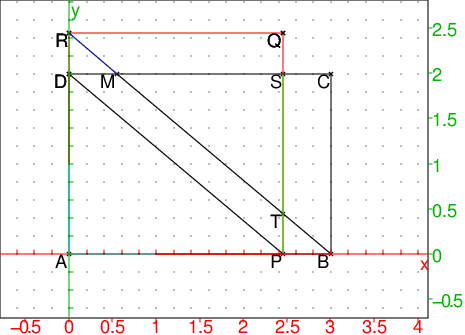
\includegraphics[width=\textwidth]{csarresqrt22}\\
Les triangles $RQP$ et $MCB$ sont \'egaux,\\ 
les triangles $RDM$ et $TPB$ sont \'egaux,
donc les 3 pi\`eces du puzzle sont les triangles $MCB$ et $TPB$ et le polygone
$APTMD$.\\
Puis on tape :
\begin{verbatim}
c:=3;
P1:=polygone(A,P,T,M,D,affichage=1+rempli);
T2:=triangle(T,P,B,affichage=2+rempli);
T4:=triangle(M,C,B,affichage=4+rempli);
affichage(translation(-c*i,P1),1+rempli)
affichage(translation(-sqrt(a*b)-c*i+a*i,T2),2+rempli);
affichage(translation(sqrt(a*b)-b-c*i+(sqrt(a*b)-a)*i,T4),
          4+rempli);
\end{verbatim}
On obtient les 3 pi\`eces du puzzle du rectangle $3*2$ :\\
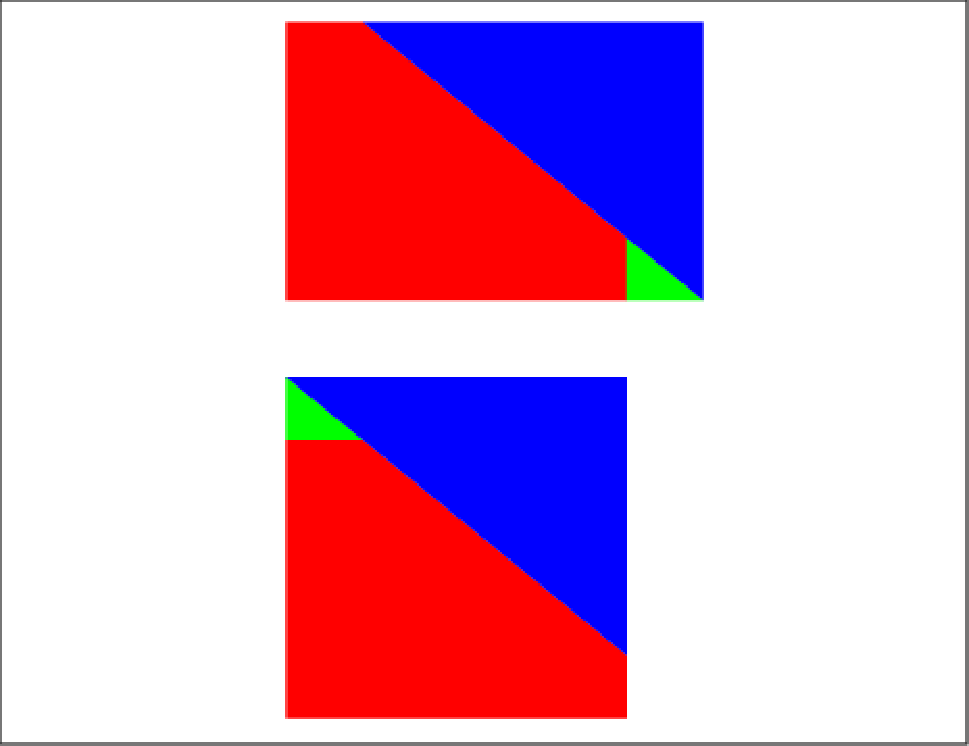
\includegraphics[width=\textwidth]{carresqrt23}\\
{\bf Autre solution}\\
Soit un rectangle de longueur 3 unit\'es et de largeur 2 unit\'es.\\
On veut le partager en plusieurs morceaux pour pouvoir constituer avec 
tous ces morceaux un carr\'e.\\
On prend exemple sur le d\'ecoupage pr\'ec\'edent.\\
Le carr\'e doit avoir comme c\^ot\'e $\sqrt 6$ unit\'es.\\
$\sqrt 6$ est l'hypot\'enuse d'un triangle rectangle de c\^ot\'e 1 et 
$\sqrt 5$ (puisque $6=1+5=1^2+(\sqrt 5)^2=(\sqrt 6)^2$.\\
On utilise la formule :\\
$2*\sqrt 5+(\sqrt 5-1)^2=6$ et\\
Dans le rectangle $2*\$sqrt 5$, on d\'ecoupe 4 triangles rectangles qui ont des 
c\^ot\'es de l'angle droit de longueur et 1 et $\sqrt 5$. \\
Il reste ensuite \`a d\'ecouper le rectangle $(3-\sqrt 5)*2$ en 3 morceaux pour
en faire un carr\'e selon la m\'ethode de la section \ref{sec:carreab}.\\
rappelons ce d\'ecoupage sur cet exemple.\\
On tape :
\begin{verbatim}
b:=2;a:=3-sqrt(5);
A:=point(0);
B:=point(b);
C:=point(b+i*a);
D:=point(i*a);
rectangle(A,B,C,D);
P:=point(sqrt(a*b));
M:=point(b-sqrt(a*b)+i*a);
Q:=point(sqrt(a*b)*(1+i));
R:=point(sqrt(a*b)*i);
S:=point(sqrt(a*b)+i*a);
T:=point(sqrt(a*b)+i*(sqrt(a*b)-a));
carre(A,P,Q,R, affichage=rouge);
segment(P,D);
segment(B,M);
segment(R,M,affichage=bleu);
segment(P,S, affichage=vert);
\end{verbatim}
Puis on tape :
\begin{verbatim}
P1:=rotation(0,pi/2,polygone(A,P,T,M,D)):;
affichage(P1,1+rempli);
T2:=rotation(0,pi/2,triangle(T,P,B)):;
affichage(T2,2+rempli);
T4:=rotation(0,pi/2,triangle(M,C,B)):;
affichage(T4,4+rempli);
affichage(translation(2,P1),1+rempli);
affichage(translation(-1+sqrt(5)-sqrt(5)*i+i,T2),2+rempli);
affichage(translation(6-2*sqrt(5)+(sqrt(5)-3)*i,T4),4+rempli);
\end{verbatim}
On obtient avec les 3 pi\`eces qui formeront le carr\'e central :\\
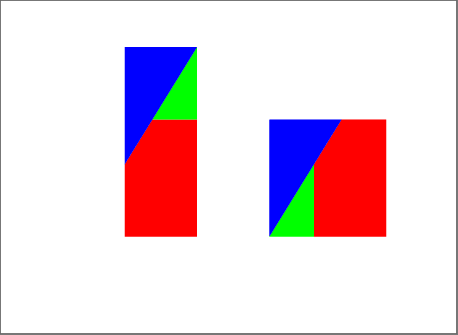
\includegraphics[width=\textwidth]{carresqrt36}\\
Pour faire les 7 morceaux, on tape :
\begin{verbatim}
rectangle(0,3,2/3):;
T1:=triangle(0,sqrt(5),i):;
affichage(T1,1+rempli);
T2:=triangle(i+sqrt(5),sqrt(5),i):;
affichage(T2,2+rempli);
T3:=triangle(i,sqrt(5)+i,2*i):;
affichage(T3,3+rempli);
T4:=triangle(2*i,sqrt(5)+2*i,i+sqrt(5)):;
affichage(T4,4+rempli);
T5:=polygone(sqrt(5),3, 3+i*(sqrt(5)-1), 
    i*(sqrt(5)-1)+7-2*sqrt(5), i*(3-sqrt(5))+sqrt(5)):;
affichage(T5,5+rempli);
T6:=triangle(3+2*i,2*i+sqrt(5),sqrt(5)+i*(3-sqrt(5))):;
affichage(T6,6+rempli);
T7:=triangle(3+i*(sqrt(5)-1),3+2*i,i*(sqrt(5)-1)+7-2*sqrt(5)):;
affichage(T7,47+rempli);
affichage(translation(-2*i-i/2,T5),5+rempli);
affichage(translation(4-2*sqrt(5)+sqrt(5)*i-5*i-i/2,T6),6+rempli);
affichage(translation(-3+sqrt(5)-sqrt(5)*i-i-i/2,T7),47+rempli);
affichage(translation(sqrt(5)*i-3*i-sqrt(5)+4-i/2,T1),1+rempli);
affichage(translation(-sqrt(5)+3-3*i-i/2,T2),2+rempli);
affichage(translation(-3*i-sqrt(5)+4-i/2,rotation(i,pi/2,T3)),
          3+rempli));
affichage(translation(3-sqrt(5)+sqrt(5)*i-5*i-i/2,
                rotation(sqrt(5)+2*i,pi/2,T4)),4+rempli));
\end{verbatim}
On obtient les 7 pi\`eces du puzzle du rectangle $3*2$ :\\
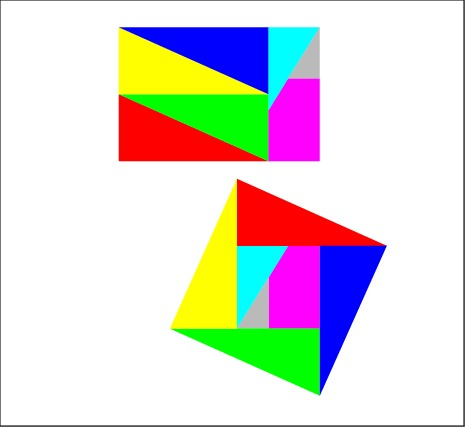
\includegraphics[width=10cm]{carresqrt67}\\
{\bf Autre solution}\\
On fait 2  triangles rectangles ($T1 et T2$) de c\^ot\'es $\sqrt 2$,2,$\sqrt 6$,
 puis on fait 2 triangles rectangle ($T5 et T6$) pour constituer le carr\'e 
central de c\^ot\'e $2-\sqrt 2$. Puis on compl\`ete en respectant la sym\'etrie.
On obtient 10 morceaux, on tape :
\begin{verbatim}
rectangle(0,3,2/3):;
T1:=triangle(0,2,sqrt(2)*i):;
affichage(T1,1+rempli);
T2:=triangle(3+2*i,1+2*i,3+(2-sqrt(2))*i):;
affichage(T2,2+rempli);
T3:=triangle(sqrt(2)*i+2-sqrt(2),sqrt(2)*i,2):;
affichage(T3,3+rempli);
T4:=triangle(1+2*i,1+sqrt(2)+(2-sqrt(2))*i,3+(2-sqrt(2))*i):;
affichage(T4,4+rempli);
T5:=triangle(sqrt(2)*i,2*i,2-sqrt(2)+sqrt(2)*i):;
affichage(T5,5+rempli);
T6:=triangle(3+(2-sqrt(2))*i,3,(2-sqrt(2))*i+sqrt(2)+1):;
affichage(T6,6+rempli);
T7:=triangle(2*i,1+2*i,1+i):;
affichage(T7,47+rempli);
T8:=triangle(1+2*i,1+i,2+i):;
affichage(T8,178+rempli);
T9:=triangle(2+i,1+i,2):;
affichage(T9,69+rempli);
T0:=triangle(2+i,3,2):;
affichage(T0,80+rempli);
affichage(translation(4.5,T1),1+rempli);
affichage(translation(4.5,
          rotation(sqrt(2)*i,-pi/2,T3)),3+rempli);
affichage(translation(4.5-2*i,T5),5+rempli);
affichage(translation(3.5-sqrt(2)-(2-sqrt(2))*i,T6),6+rempli);
affichage(translation(3.5-sqrt(2)-4*i+sqrt(2)*i,T2),2+rempli);
affichage(translation(3.5-sqrt(2)-4*i+sqrt(2)*i,
          rotation(3+(2-sqrt(2))*i,-pi/2,T4)),4+rempli);
affichage(translation(3.5-sqrt(2)/2-4*i+3*sqrt(2)/2*i,
          rotation(1+2*i,pi/4,T7)),47+rempli);
affichage(translation(3.5-sqrt(2)/2-3*i+3*sqrt(2)/2*i,
          rotation(1+i,-pi/4,T8)),178+rempli);
affichage(translation(4.5-sqrt(2)/2-i-sqrt(2)/2*i,
          rotation(2+i,-pi/4,T9)),69+rempli);
affichage(translation(4.5-sqrt(2)/2-sqrt(2)/2*i,
          rotation(2,pi/4,T0)),80+rempli);
\end{verbatim}
On obtient les 10 pi\`eces du puzzle du rectangle $3*2$ :\\
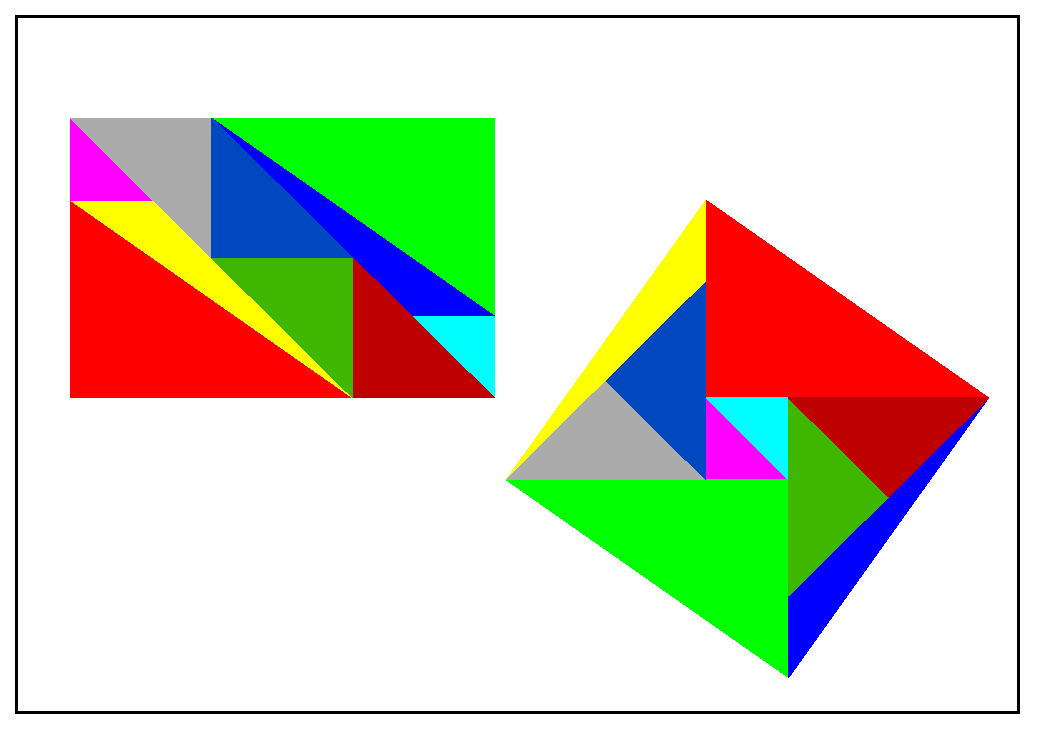
\includegraphics[width=\textwidth]{carresqrt60}



\section{Puzzle transformant un rectangle $a*(a+1)$ en un carr\'e}
Soit un rectangle de longueur $a+1$ unit\'es et de largeur $a$ unit\'es avec 
$a\geq 1$ (pour avoir $\sqrt a \leq a$).\\
On veut le partager en plusieurs morceaux pour pouvoir constituer avec 
tous ces morceaux un carr\'e.\\
On prend exemple sur le d\'ecoupage pr\'ec\'edent.\\
Le carr\'e reconstitu\'e a pour c\^ot\'e $\sqrt{a^2+a}$ unit\'es.\\
$\sqrt{a^2+a}$ est l'hypot\'enuse d'un triangle rectangle de c\^ot\'e $a$ et 
$\sqrt a$ (puisque $a^2+a=a^2+(\sqrt a)^2=(\sqrt {a^2+a})^2$.\\
On utilise la formule :\\
$2a*\sqrt a+(a-\sqrt a)^2=a^2+a$ et\\
On consid\`ere la droite $D$ d'\'equation $y=-\sqrt ax+a$ (c'est la droite
portant l'hypot\'enuse du triangle $0,\sqrt a,a$\\.
Puisque le point de coordonn\'ees $(1,a-\sqrt a)$ est sur la droite $D$, on 
peut d\'ecouper le rectangle selon les 5 morceaux ci-dessous.\\
Voici ce puzzle fait avec ces 5 morceaux mais on remarquera qu'il suffit de 
d\'ecouper le rectangle en seulement 3 morceaux !!!\\
On tape :
\begin{verbatim}
supposons(a=[2,1.0,10.0,0.1]);
rectangle(0,a+1,a/(a+1)):;
T1:=triangle(0,sqrt(a),a*i):; affichage(T1,1+rempli);
T2:=triangle(1+a*i,1+(a-sqrt(a))*i,a+1+a*i):; 
affichage(T2,2+rempli);
T3:=triangle(a+1+a*i,1+(a-sqrt(a))*i,a+1+(a-sqrt(a))*i):; 
affichage(T3,3+rempli);
T4:=triangle(a*i,1+(a-sqrt(a))*i,1+a*i):; 
affichage(T4,4+rempli);
T5:=polygone(1+(a-sqrt(a))*i,sqrt(a),1+sqrt(a),
    1+sqrt(a)+(a-sqrt(a))*i):; 
affichage(T5,5+rempli);
T6:=carre(1+sqrt(a),a+1):;
affichage(T6,6+rempli);
carre(sqrt(a)-a,a*i-a):;
affichage(translation(-a,T1),1+rempli);
affichage(translation(-2a-1,T3),3+rempli);
affichage(translation(-2a-1,T5),5+rempli);
affichage(translation(-2a-1,T6),6+rempli);
affichage(translation(-a-1+sqrt(a)-a-a*i,T2),2+rempli);
affichage(translation(-1-a+sqrt(a)-a-a*i,T4),4+rempli);
\end{verbatim}
On obtient les 5 (ou 3) pi\`eces du puzzle du rectangle $(a+1)*a$ pour $a=4$ :\\
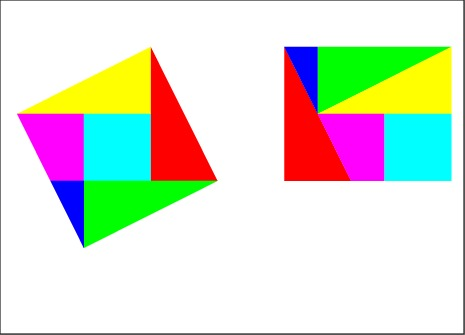
\includegraphics[width=\textwidth]{carresqrta}\\
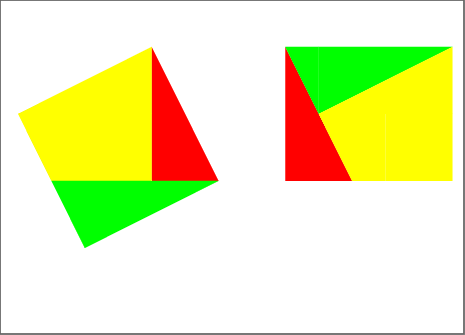
\includegraphics[width=\textwidth]{carresqrta0}\\
On obtient les 5 (ou 3) pi\`eces du puzzle du rectangle $(a+1)*a$ pour $a=10$ :\\
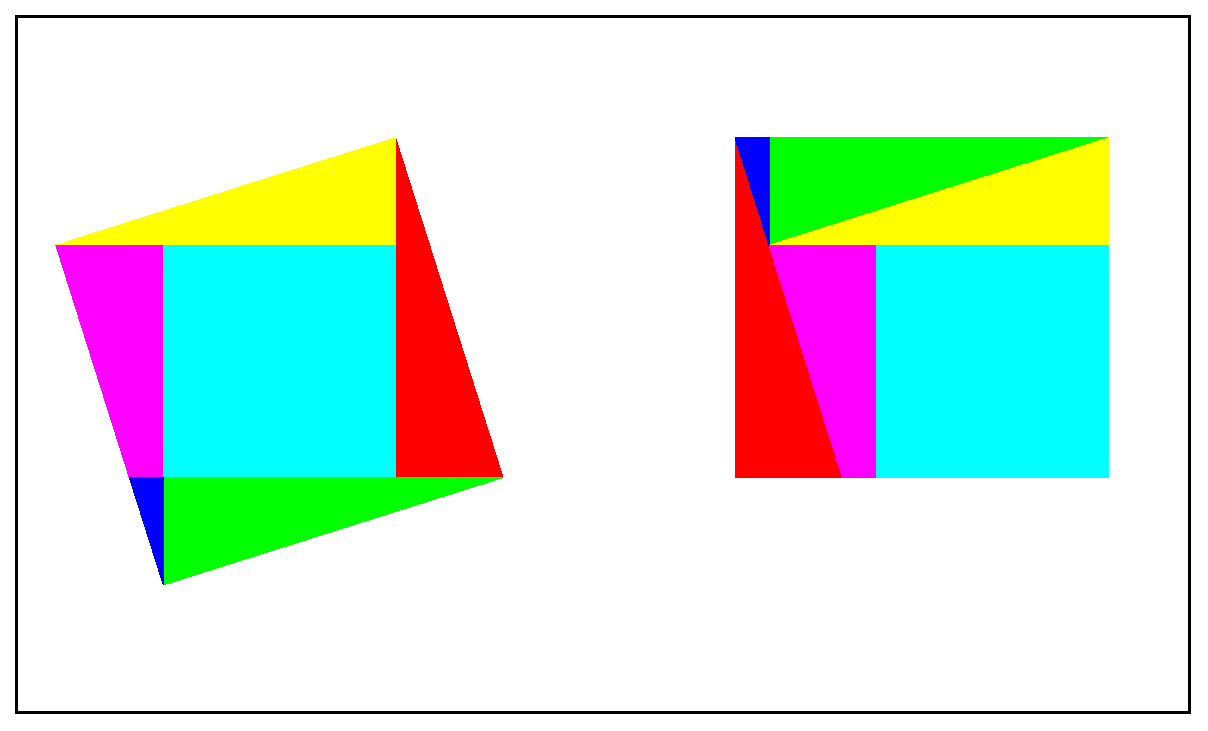
\includegraphics[width=\textwidth]{carresqrta1}
\section{Puzzle transformant un rectangle 3x1 en un carr\'e}
Soit un rectangle de longueur 3 unit\'es et de largeur 1 unit\'e.\\
On veut le partager en plusieurs morceaux pour pouvoir constituer avec 
tous ces morceaux un carr\'e.\\
Le carr\'e reconstitu\'e a pour c\^ot\'e $\sqrt 3$ unit\'es.\\
\subsection{On prend exemple sur le d\'ecoupage pr\'ec\'edent}
On utilise la formule :\\
$2*\sqrt 2+(\sqrt 2-1)^2=6$\\
Donc le carr\'e sera au centre a un c\^ot\'e de longueur $\sqrt 2-1$ unit\'es.\\
Voici ce puzzle fait avec ces 8 morceaux mais on remarquera qu'il suffit de 
d\'ecouper le rectangle en seulement 4 morceaux !!!\\
On tape :
\begin{verbatim}
rectangle(0,3,1/3):;
T1:=triangle(0,sqrt(2),i):; 
affichage(T1,1+rempli);
T2:=triangle(3,3-sqrt(2)/2,3+i):; 
affichage(T2,2+rempli);
T3:=polygone(2,2+i*(2-sqrt(2)),(2-sqrt(2))*(1+i),sqrt(2)):; 
affichage(T3,3+rempli);
T4:=polygone(2,3-sqrt(2)/2,3+i,2+i):; 
affichage(T4,4+rempli);
T5:=carre(2+i*(2-sqrt(2)),2+i):; 
affichage(T5,5+rempli);
T6:=triangle(i,(2-sqrt(2))*(1+i),2-sqrt(2)+i):; 
affichage(T6,6+rempli);
T0:=triangle(i+(2-sqrt(2))*3/2,(2-sqrt(2))*(1+i),2-sqrt(2)+i):; 
affichage(T0,rempli);
T7:=polygone((i+(2-sqrt(2))*3/2,(2-sqrt(2))*(1+i),
              3-sqrt(2)+(2-sqrt(2))*i),3-sqrt(2)+i):; 
affichage(T7,47+rempli);
affichage(translation(2-2*i+i/2,T1),1+rempli);
affichage(translation(-1-2*i+i/2,T2),2+rempli);
affichage(translation(-3i-1+i/2+sqrt(2),T7),47+rempli);
affichage(translation(-3i-1+sqrt(2)+i/2,T5),5+rempli);
affichage(translation(-1+sqrt(2)-3*i+i/2,T4),4+rempli);
affichage(translation(-1+sqrt(2)-3*i+i/2,T3),3+rempli);
affichage(translation(-1+2*sqrt(2)-4*i+i/2,T6),6+rempli);
affichage(translation(-1+2*sqrt(2)-4*i+i/2,T0),0+rempli);
\end{verbatim}
On obtient les 8 pi\`eces du puzzle du rectangle $3*1$ :\\
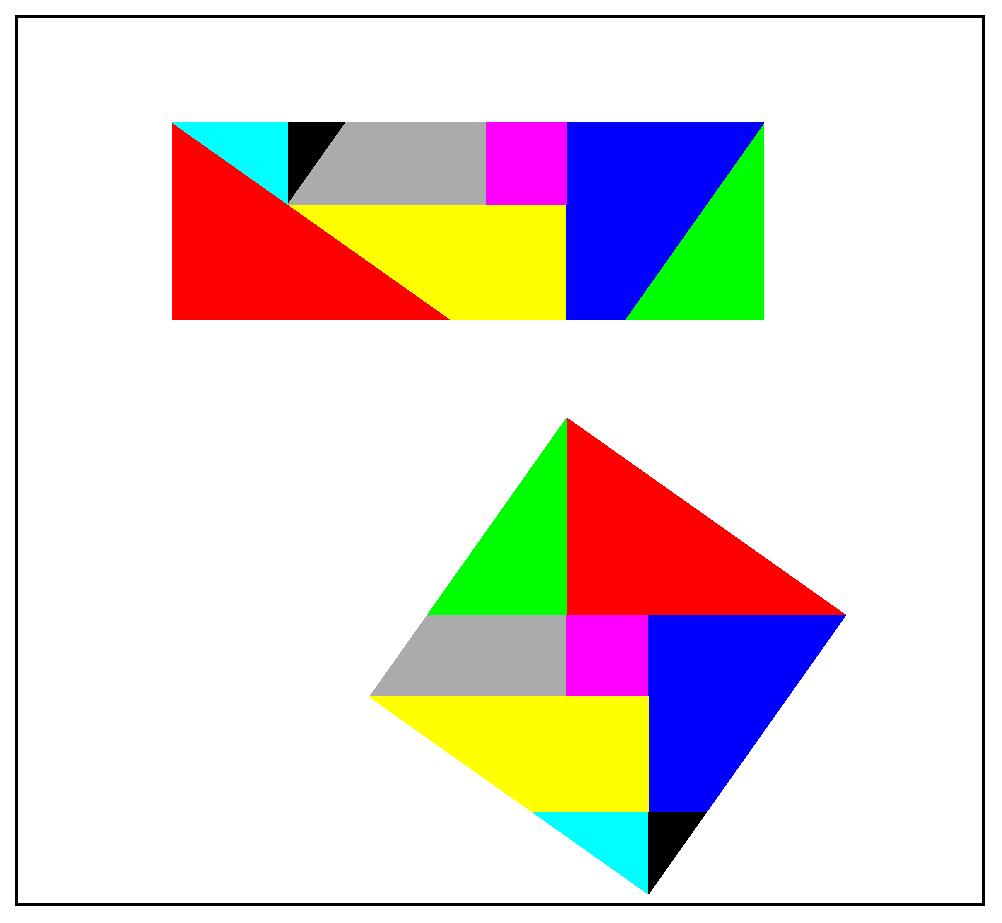
\includegraphics[width=10cm]{carresqrt30}\\
On obtient avec 5 pi\`eces :\\
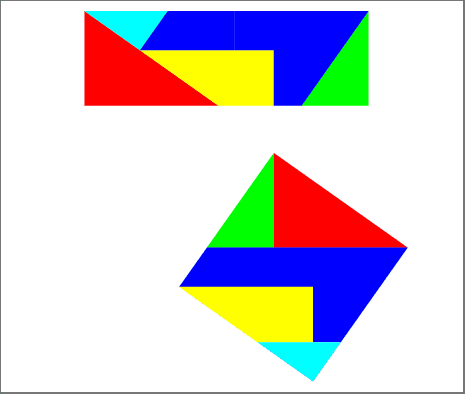
\includegraphics[width=10cm]{carresqrt35}
\subsection{Autre d\'ecoupage}
On construit donc un triangle rectangle {\tt T1} ayant comme c\^ot\'e 1 et 
$\sqrt 2$ : son hypoth\'enuse a pour longueur $\sqrt 3$.\\
{\tt T1} est le triangle $PMR$.\\
Puis on trace la perpendiculaire $NM$ \`a $PQ$.
{\tt T2} est le triangle $NMR$.\\
Le triangle {\tt T3} (resp {\tt T4}) est le sym\'etrique de {\tt T1} (resp 
{\tt T2}) par rapport au centre du rectangle.\\
Le triangle $OPR$ et son sym\'etrique  par rapport au centre du rectangle sont 
des triangles rectangles isoc\`eles (leurs c\^ot\'es sont de longueur 1,1 et 
$\sqrt 2$).\\
Le triangle $NMQ$ et son sym\'etrique  par rapport au centre du rectangle sont 
des triangles rectangles isoc\`eles (leurs  c\^ot\'es sont de longueur  
$\sqrt 2 -1$, $\sqrt 2 -1$, 2-$\sqrt 2$).\\
On tape :
\begin{verbatim}
rectangle(-4,-1,1/3);
segment(-2,-2+i,affichage=ligne_tiret_pointpoint);
segment(-3,-3+i,affichage=ligne_tiret_pointpoint);
T1:=triangle(-4+i,-3,-3+(1+i)/sqrt(2));
O:=point(-4);
M:=point(-3+(1+i)/sqrt(2),affichage=quadrant4);
N:=point(-4+sqrt(2)+i,affichage=quadrant2);
P:=point(-3);
Q:=point(-2+i,affichage=quadrant2);
R:=point(-4+i,affichage=quadrant2);
T2:=triangle(-4+i,-3+(1+i)/sqrt(2),-4+sqrt(2)+i);
T3:=symetrie(point(-5/2+i/2),T1);
T4:=symetrie(point(-5/2+i/2),T2);
\end{verbatim}
On obtient les 8 pi\`eces triangulaires qui pavent le rectangle $3*1$  :\\
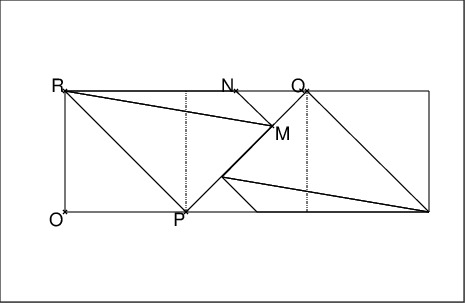
\includegraphics[width=11cm]{carresqrt}\\
On r\'ealise le puzzle.\\
On tape :
\begin{verbatim}
rectangle(-4,-1,1/3):;
T1:=triangle(-4+i,-3,-3+(1+i)/sqrt(2)):;T1;
T2:=triangle(-4+i,-3+(1+i)/sqrt(2),-4+sqrt(2)+i):;
T3:=symetrie(point(-5/2+i/2),T1):;T3;
T4:=symetrie(point(-5/2+i/2),T2):;
translation(3/2-3/2*i,T1,affichage=1+rempli);
R2:=rotation(-3+(1+i)/sqrt(2),pi/2,T2):;T2;
translation(3/2-3/2*i,R2,affichage=2+rempli);
A:=translation(3/2-3/2*i,rotation(-3+(1+i)/sqrt(2),pi/2,-4+i)):;
translation(affixe(A)+1,T3,affichage=3+rempli);
R4:=rotation(-2-1/sqrt(2)+i*(1-1/sqrt(2)),pi/2,T4):;
translation(affixe(A)+1,R4,affichage=4+rempli);
triangle(A,A+sqrt(2)*i,A+(i-1)/sqrt(2),affichage=5+rempli);
B:=translation(affixe(A)+1,rotation(-2-1/sqrt(2)+i*(1-1/sqrt(2)),
              pi/2,point(-1))):;
triangle(B,B-i*sqrt(2),B+(1-i)/sqrt(2),affichage=6+rempli);
segment(B+(1-i)/sqrt(2),A+(i-1)/sqrt(2));
affichage(T1,1+rempli);
affichage(T2,2+rempli);
affichage(T3,3+rempli);
affichage(T4,4+rempli);
T5:=triangle(-1,-1+i,-2+i):;
affichage(T5,5+rempli);
T6:=triangle(-4,-3,-4+i):;
affichage(T6,6+rempli);
T7:=triangle(-3,-1-sqrt(2),-2-1/sqrt(2)+i*(1-1/sqrt(2))):;
affichage(T7,47+rempli);
T0:=triangle(-2+i,-4+sqrt(2)+i,-3+1/sqrt(2)+i*(1/sqrt(2))):;
affichage(T0,rempli);
triangle(-3/2-3*i/2,B+(1-i)/sqrt(2),A+(i-1)/sqrt(2),affichage=rempli);
triangle(-7/2+sqrt(2)-3*i/2,B+(1-i)/sqrt(2),A+(i-1)/sqrt(2),
         affichage=47+rempli);
\end{verbatim}
On obtient les 8 pi\`eces du puzzle du rectangle $3*1$ :\\
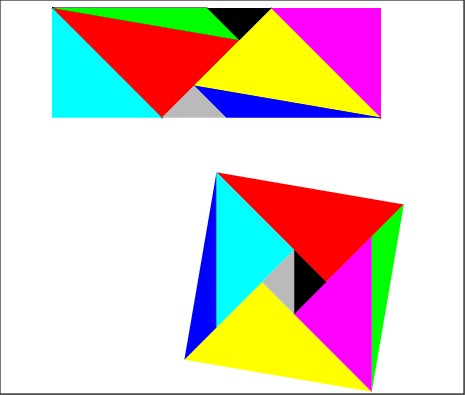
\includegraphics[width=\textwidth]{carresqrt3}
\subsection{Autre d\'ecoupage}
On utilise la formule :\\
$\sqrt(3)^2+1^2=2^2$\\
Soit $ABCD$ un rectangle de dimension $1*3$.\\
Soit $APQR$ un carr\'e de dimension $\sqrt 3$.\\
On dessine donc 2 triangles rectangles $APD$ et $BCM$ dont les c\^ot\'es de 
l'angle droit ont pour longueur 1 et $\sqrt 3$.\\
On tape :
\begin{verbatim}
A:=point(0);
B:=point(3);
C:=point(3+i);
D:=point(i);
rectangle(A,B,C,D);
P:=point(sqrt(3));
M:=point(3-sqrt(3)+i);
Q:=point(sqrt(3)*(1+i));
R:=point(sqrt(3)*i);
S:=point(sqrt(3)+i);
T:=point(sqrt(3)+i*(sqrt(3)-1));
carre(A,P,Q,R, affichage=rouge);
segment(P,D);
segment(B,M);
segment(R,M,affichage=bleu);
segment(P,S, affichage=vert);
\end{verbatim}
On obtient :\\
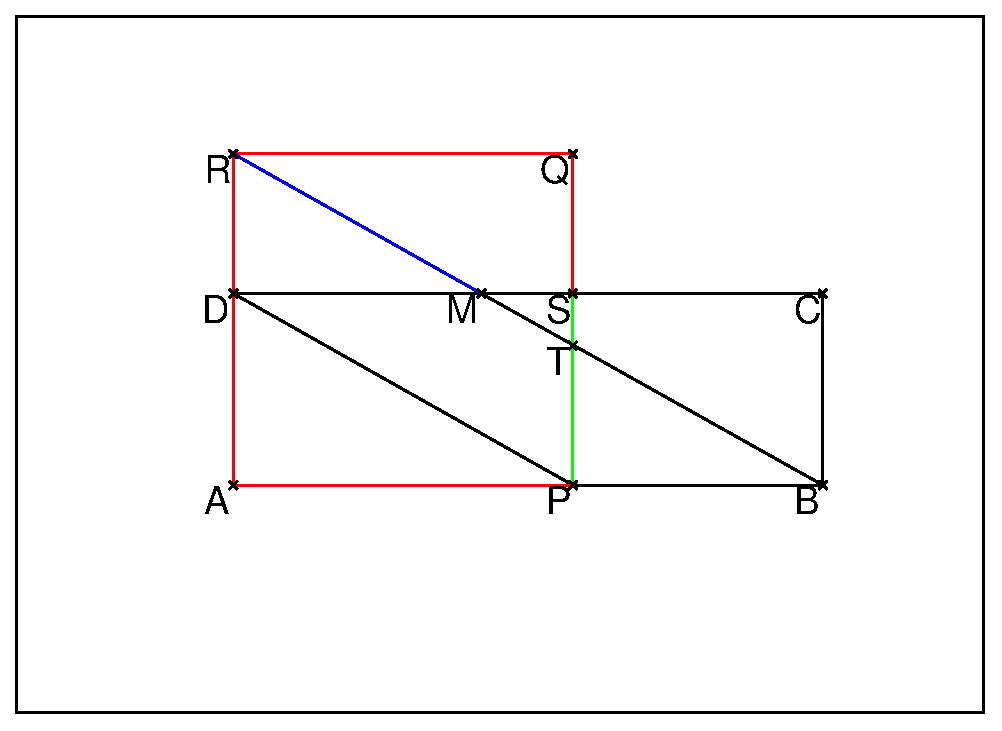
\includegraphics[width=11cm]{carresqrt31}\\
Les points $B,M,R$ sont align\'es car les droites $BR$ et $BM$ ont m\^eme pente
qui vaut $\frac{\sqrt 3}{3}=\frac{1}{\sqrt 3}$.\\
Les triangles rectangles $BCM$ et $TQR$ sont \'egaux ($CM=QR=\sqrt 3$ et leurs 
angles sont \'egaux).\\
Le point $T$ intersection de $BR$ et $PQ$ a pour coordonn\'ees :\\
$\sqrt 3,\sqrt 3 -1$ puisque :\\
$PT/PB=\frac{PT}{3-\sqrt 3}=AR/AB=\frac{\sqrt 3}{3}$
on a $PT=\sqrt 3-1$\\
Les triangles rectangles $PBT$ et $DMR$ sont donc \'egaux ($PT=DR=\sqrt 3-1$ et 
leurs angles sont \'egaux).\\
On tape :\\
\begin{verbatim}
P1:=polygone(A,P,T,M,D,affichage=1+rempli);
T2:=triangle(T,P,B,affichage=2+rempli);
T4:=triangle(M,C,B,affichage=4+rempli)
affichage(translation(-2*i,P1),1+rempli)
affichage(translation(-sqrt(3)-i,T2),2+rempli);
affichage(translation((sqrt(3)-3)*(1+i),T4),4+rempli);
\end{verbatim}
On obtient donc 3 pi\`eces :\\
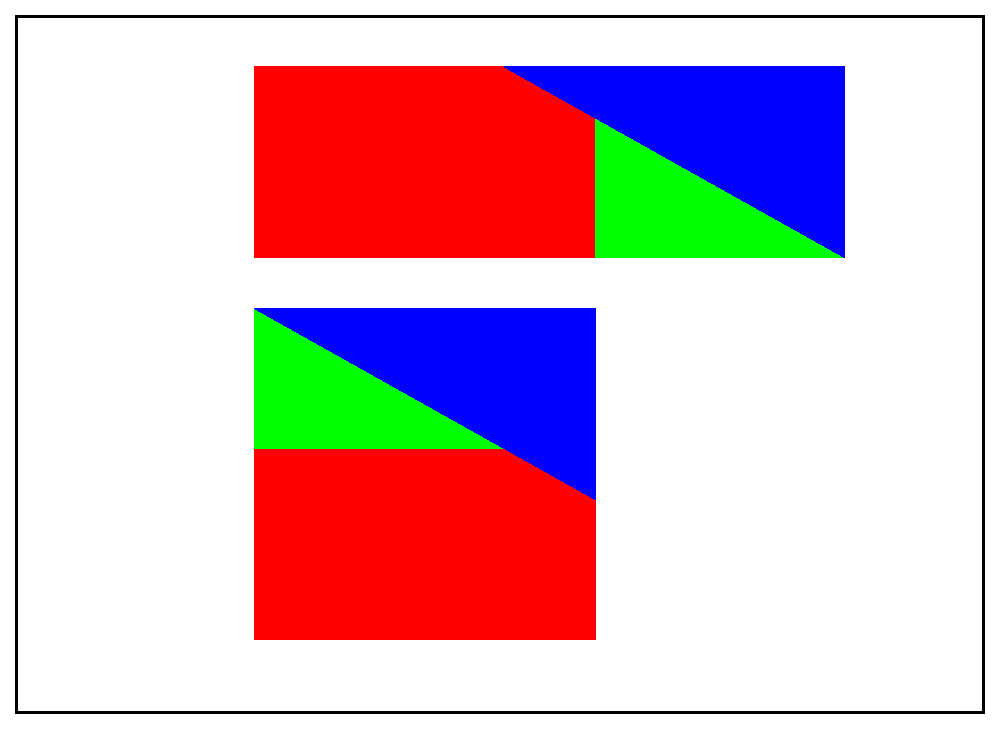
\includegraphics[width=\textwidth]{carresqrt32}\\

On peut faire 4 pi\`eces.\\
On tape :\\
\begin{verbatim}
affichage(triangle(A,P,D),3+rempli);
affichage(translation(-2*i,triangle(A,P,D)),3+rempli);
\end{verbatim}
On obtient les 3 pi\`eces du puzzle du rectangle $3*1$ :\\
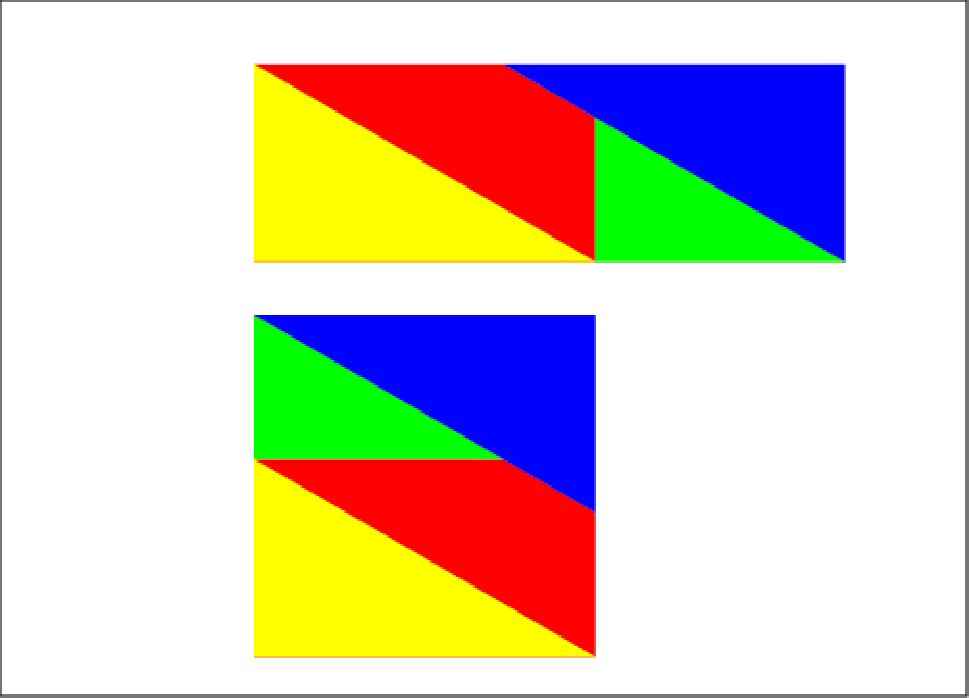
\includegraphics[width=\textwidth]{carresqrt34}\\
Dans la section suivante on fait une g\'en\'eralisation de ce d\'ecoupage \`a 
condition que la longueur du rectangle soit inf\'erieure \`a 4 fois sa largeur.
\section{Puzzle transformant un rectangle $a*b$ en un carr\'e}\label{sec:carreab}
Soit un rectangle de longueur $b$ unit\'es et de largeur $a$ unit\'es avec 
$a\leq b \leq 4a$.\\
On veut le partager en plusieurs morceaux pour pouvoir constituer avec 
tous ces morceaux un carr\'e.\\
On prend exemple sur le d\'ecoupage pr\'ec\'edent du rectangle 1x3.\\
Le carr\'e reconstitu\'e a pour c\^ot\'e $\sqrt{ab}$ unit\'es.\\
On consid\`ere le rectangle $ABCD$ ($AD=a$ et $AB=\sqrt{ab}$.\\
 Soit $APQR$ un carr\'e de dimension $\sqrt{ab}$.\\
On dessine donc 2 triangles rectangles $APD$ et $BCM$ ayant comme c\^ot\'es de 
l'angle droit $a$ et $\sqrt{ab}$.\\
On tape :
\begin{verbatim}
supposons(a=[2,0.0,10.0,0.1]);
supposons(b=[2,a,4*a.0,0.1]);
A:=point(0);
B:=point(b);
C:=point(b+i*a);
D:=point(i*a);
rectangle(A,B,C,D);
P:=point(sqrt(a*b));
M:=point(b-sqrt(a*b)+i*a);
Q:=point(sqrt(a*b)*(1+i));
R:=point(sqrt(a*b)*i);
S:=point(sqrt(a*b)+i*a);
T:=point(sqrt(a*b)+i*(sqrt(a*b)-a));
carre(A,P,Q,R, affichage=rouge);
segment(P,D);
segment(B,M);
segment(R,M,affichage=bleu);
segment(P,S, affichage=vert);
\end{verbatim}
On obtient les 3 pi\`eces du puzzle du rectangle $b*a$ (pour $a=1.5$ et $b=4$) :\\
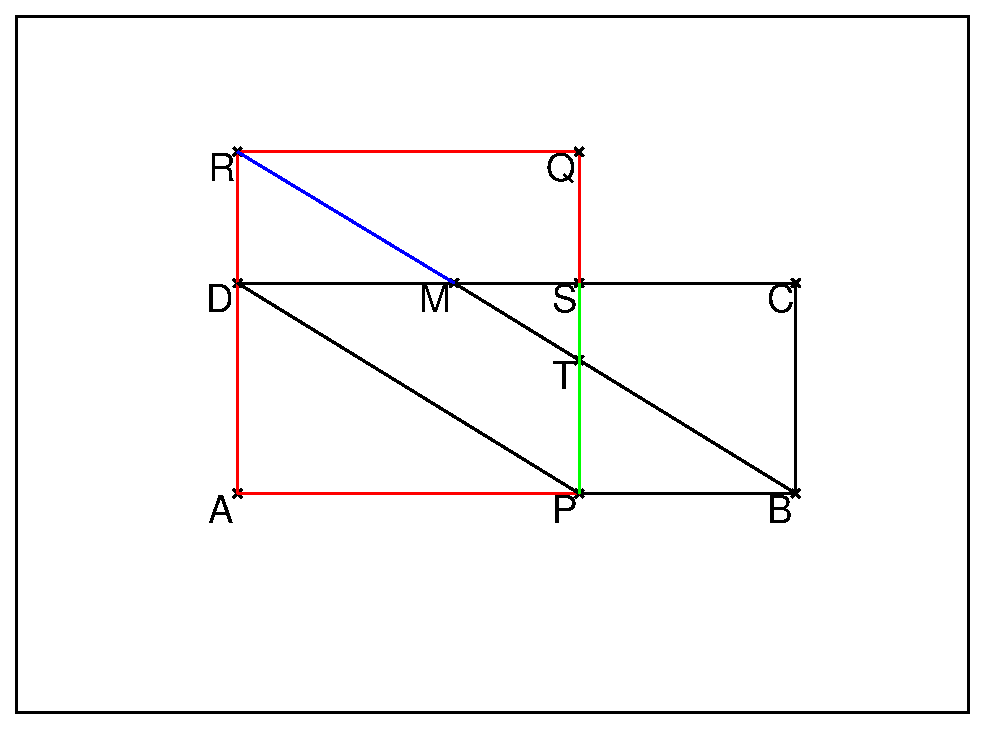
\includegraphics[width=8cm]{carresqrta2}\\
Les points $BMR$ sont align\'es car les droites $BR$ et $BM$ ont m\^eme 
pente car $\frac{a}{\sqrt{a*b}}=\frac{\sqrt{a*b}}{b}$.\\
Les triangles rectangles $BCM$ et $TQR$ sont \'egaux ($CM=QR=\sqrt{ab}$ et 
leurs angles sont \'egaux).\\
Le point $T$ intersection de $BR$ et $PQ$ a pour coordonn\'ees :\\
$\sqrt{ab},\sqrt{ab} -a$ puisque :\\
$PT/PB=\frac{PT}{b-\sqrt{ab}}=AR/AB=\frac{\sqrt{ab}}{b}$
on a $PT=\sqrt{ab}-a$\\
Pour que  $T$ soit sur le segment $PS$ on suppose que $PT=\sqrt{ab}-a\leq a$
c'est \`a dire $a\leq b\leq 4a$.\\
Les triangles rectangles $PBT$ et $DMR$ sont donc \'egaux ($PT=DR=\sqrt{ab}-a$ 
et leurs angles sont \'egaux).\\
On tape en notant $c$ le param\`etre qui produit la translation 
$-c*i$ de la pi\`ece rouge :\\
\begin{verbatim}
supposons(a=[2,0.0,10.0,0.1]);
supposons(b=[2,a,4*a.0,0.1]);
supposons(c=[2,0.0,10.0,0.1]);
P1:=polygone(A,P,T,M,D,affichage=1+rempli);
T2:=triangle(T,P,B,affichage=2+rempli);
T4:=triangle(M,C,B,affichage=4+rempli);
affichage(translation(-c*i,P1),1+rempli)
affichage(translation(-sqrt(a*b)-c*i+a*i,T2),2+rempli);
affichage(translation(sqrt(a*b)-b-c*i+(sqrt(a*b)-a)*i,T4),
          4+rempli);
\end{verbatim}
On obtient donc 3 pi\`eces du rectangle $b*a$ pour $a=1.5,b=3.1,c=2.5$ :\\
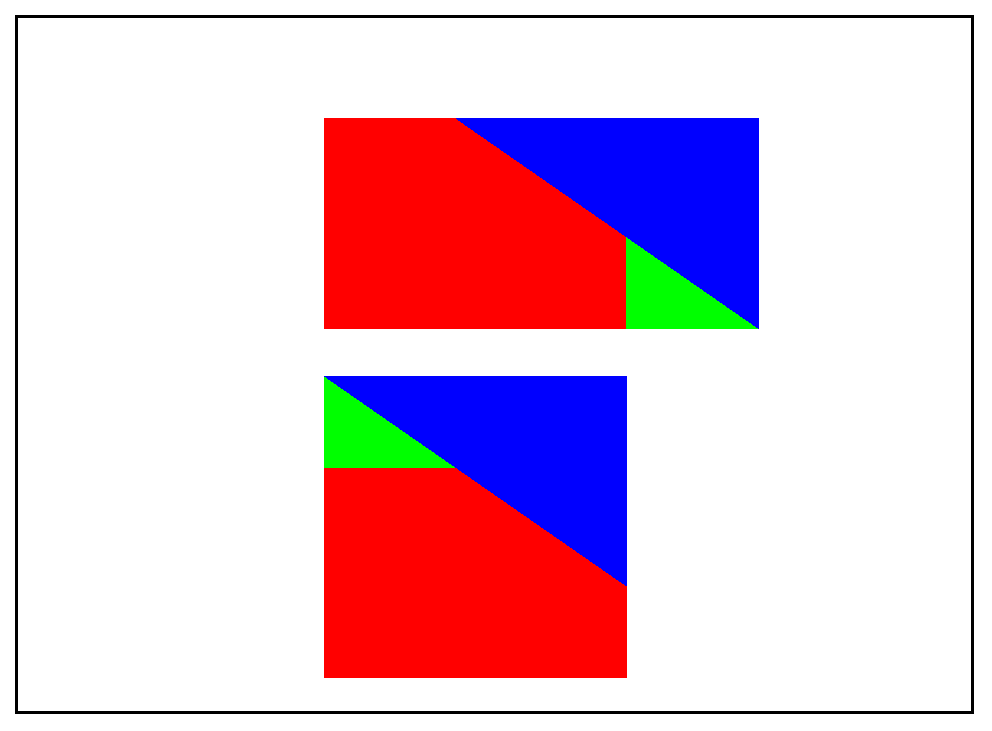
\includegraphics[width=\textwidth]{carresqrta3}

\section{Exercice}
Faire un puzzle qui transforme un rectangle 1*6 en un carr\'e.\\
{\bf Une solution}: \\
Comme 6>4*1, on ne peut pas utiliser le d\'ecoupage 
 ci-dessus en 3 morceaux.
On d\'ecoupe le rectangle en 2 morceaux de 1*3, puis on fait le d\'ecoupage 
en 3 pi\`eces d'un rectangle 2*3 : cela fait 5 pi\`eces pour le rectangle 1*6.\\
 On tape :
\begin{verbatim}
rectangle(0,3,2/3);
triangle(3,3+2*i,3-sqrt(6)+2*i);
carre(0,sqrt(6));
segment(i*sqrt(6),3);
T1:=polygone(i,0,sqrt(6),sqrt(6)+i*(sqrt(6)-2),i+3-sqrt(6)/2):;
affichage(T1,1+rempli);
T2:=triangle(3,3+i,3-sqrt(6)/2+i):;
affichage(T2,2+rempli);
T3:=triangle(sqrt(6),3,sqrt(6)+i*(sqrt(6)-2)):;
affichage(T3,3+rempli);
T4:=polygone(6,6+i,6+i-sqrt(6),6-sqrt(6)/2):;
affichage(T4,4+rempli);
T5:=polygone(i+3,3,6-sqrt(6)/2,i+6-sqrt(6)):;
affichage(T5,5+rempli);
affichage(translation(-3*i,T1),1+rempli);
affichage(translation(sqrt(6)-3+sqrt(6)*i-5*i,T2),2+rempli);
affichage(translation(-sqrt(6)-i,T3),3+rempli);
affichage(translation(-6+sqrt(6)+sqrt(6)*i-4*i,T4),4+rempli);
affichage(translation(-3-2*i,T5),5+rempli);
\end{verbatim}
On obtient donc 5 pi\`eces :\\
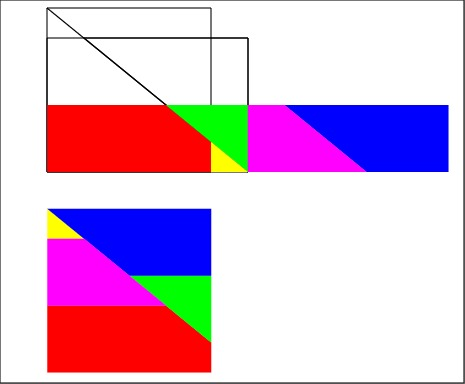
\includegraphics[width=\textwidth]{carresqrt61}
{\bf Une autre solution} : \\
On d\'ecoupe le rectangle en 2 morceaux de 1*3, puis on fait le d\'ecoupage 
en 3 pi\`eces d'un rectangle $a*(a+1)$ avec $a=2$ : cela fait 6 pi\`eces pour 
le rectangle 1*6.\\
 On tape :
\begin{verbatim}
T1:=polygone(0,sqrt(2),sqrt(2)/2+i,i):;
affichage(T1,1+rempli);
T4:=triangle(3,3+sqrt(2)/2,3+i):;
affichage(T4,4+rempli);
T2:=triangle(1+(2-sqrt(2))*i,3-sqrt(2)+i,sqrt(2)/2+i):;
affichage(T2,2+rempli);
T3:=polygone(sqrt(2),3,3+i,3-sqrt(2)+i,1+(2-sqrt(2))*i):;
affichage(T3,3+rempli);
T5:=triangle(6-sqrt(2),6,6+i):;
affichage(T5,5+rempli);
T6:=polygone(6-sqrt(2),6+i,3+i,3+sqrt(2)/2):;
affichage(T6,6+rempli);
affichage(translation(3-2*i-i/2,T1),1+rempli);
affichage(translation(-i-i/2,T4),4+rempli);
affichage(translation(-3+sqrt(2)-3*i-i/2,T6),6+rempli);
affichage(translation(sqrt(2)+-4*i-i/2,T2),2+rempli);
affichage(translation(-2*i-i/2,T3),3+rempli);
affichage(translation(-3-i-i/2,T5),5+rempli);
\end{verbatim}
On obtient donc 6 pi\`eces :\\
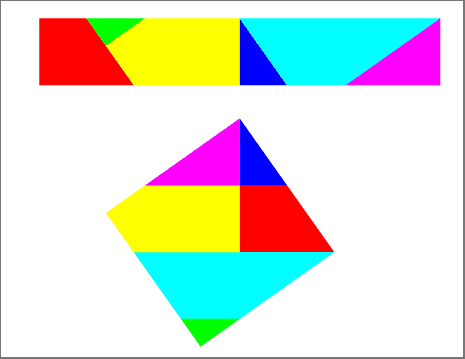
\includegraphics[width=\textwidth]{carresqrt62}
{\bf Encore une autre solution} : \\
On utilise le d\'ecoupage en 3 morceaux en le modifant : on rajoute un 
quatri\`eme morceau pour que le porc\'ed\'e marche encore quand $4=4a<b=6<8a=8$.\\
On tape :
\begin{verbatim}
rectangle(0,6,1/6);
carre(0,sqrt(6));
segment(6,sqrt(6)*i);
segment(i*2,6-2*sqrt(6)+i*2);
segment(2*sqrt(6),2*sqrt(6)+i*(sqrt(6)-2));
T1:=polygone(0,sqrt(6),sqrt(6)+i,i):;
T2:=polygone(sqrt(6)+i,sqrt(6),2*sqrt(6),
             2*sqrt(6)+i*(sqrt(6)-2),6-sqrt(6)+i):;
T3:=triangle(6,6+i,6-sqrt(6)+i):;
T4:=triangle(2*sqrt(6),6,2*sqrt(6)+i*(sqrt(6)-2)):;
affichage(T1,1+rempli);
affichage(T2,2+rempli);
affichage(T3,3+rempli);
affichage(T4,4+rempli);
\end{verbatim}
On obtient :\\
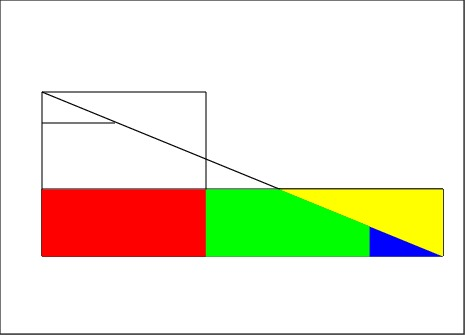
\includegraphics[width=10cm]{carresqrt65}\\
La droite d'\'equation $y=-\sqrt 6/6*x+sqrt(6)$ d\'etermine un petit triangle 
rectangle (en noir) qui se trouve \`a l'ext\'erieur du rectangle et du carr\'e.
Ce triangle a pour c\^ot\'e de l'angle droit : $6-2\sqrt 6$ et $\sqrt 6-2$.
On le translate dans le rectangle (en bleu) et dans le carr\'e.
On obtient donc les 4 pi\`eces ci dessus.\\
On r\'ealise le puzzle avec ces 4 pi\`eces, on tape :
\begin{verbatim}
affichage(T1,1+rempli);
affichage(T2,2+rempli);
affichage(T3,3+rempli);
affichage(T4,4+rempli);
affichage(translation(1.5*i,T1),1+rempli);
affichage(translation(2.5*i-sqrt(6),T2),2+rempli);
affichage(translation(sqrt(6)*i+0.5*i-6+sqrt(6),T3),3+rempli);
affichage(translation(3.5*i-2*sqrt(6),T4),4+rempli);
\end{verbatim}
On obtient :\\
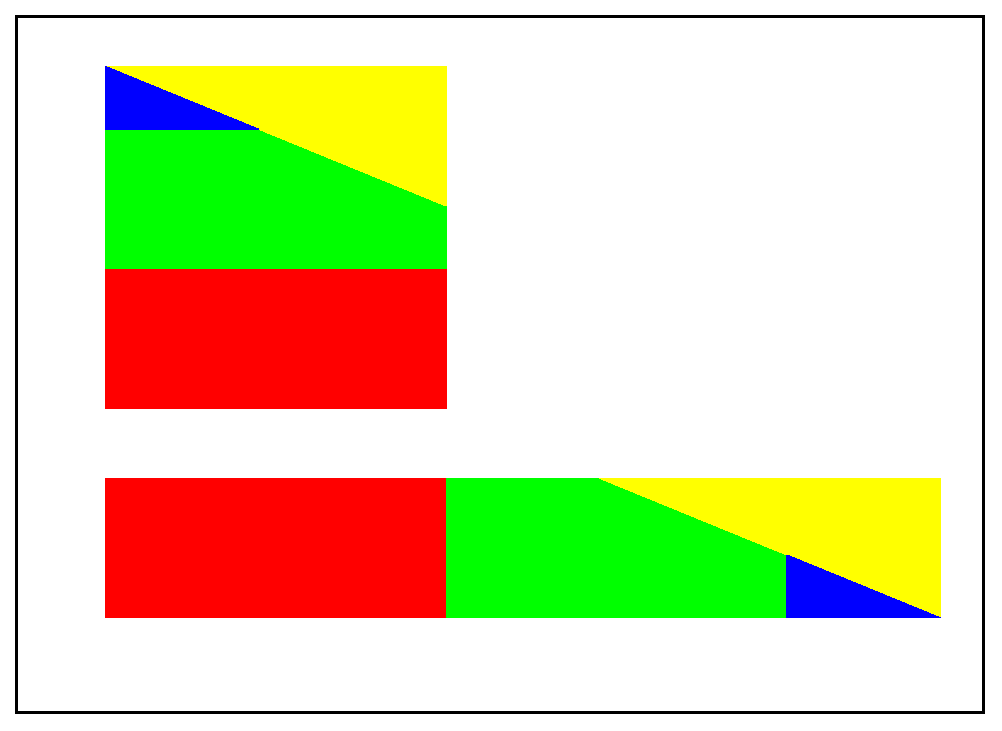
\includegraphics[width=10cm]{carresqrt66}
\section{La quadrature d'un triangle \'equilat\'eral}
\subsection{Le carr\'e, le rectangle $1*\sqrt3$ et le triangle \'equilat\'eral avec 8 et 6 pi\`eces}
On peut transformer un rectangle de dimension $a*b$ en un triangle isoc\`ele 
\`a l'aide de 4 pi\`eces : 2 triangles rectangles et 2 trap\`ezes rectangles.\\
Le triangle est obtenu en faisant subir au triangle $LDU$ (resp $NUA$) une 
rotation de centre $L$ (resp $N$) et d'angle $\pi$ : le triangle a comme base 
de longueur $2*a$ et la hauteur reli\'ee \`a cette base a pour longueur $b$.\\
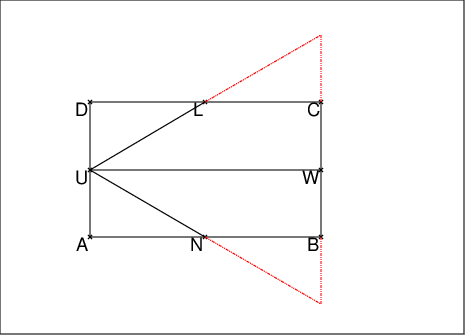
\includegraphics[width=8cm]{puzzleca0}\\
{\bf Remarques}
On peut aussi de la m\^eme fa\c{c}on transformer un rectangle de dimension 
$a*b$ en un triangle isoc\`ele de base $2*b$ et de hauteur $a$ relative \`a 
cette base.\\
On remarquera aussi qu'il suffit de 3 pi\`eces pour r\'ealiser cette 
transformation (le partage $UW$ etant inutile !).\\
\`A condition que les angles de la base $b$ soient aigus, tout triangle de base
$b$ et de hauteur $2*a$ relative \`a cette base se transforme de cette fa\c{c}on
en un rectangle $a*b$.

On va donc transformer selon cette m\`ethode un rectangle $1*\sqrt3$ en un 
triangle \'equilat\'eral et en un carr\'e.\\
On tape :
\begin{verbatim}
b:=sqrt(3);a:=1;
A:=point(0);
B:=point(b);
C:=point(b+i*a);
D:=point(i*a);
rectangle(A,B,C,D);
P:=point(sqrt(a*b));
M:=point(b-sqrt(a*b)+i*a);
Q:=point(sqrt(a*b)*(1+i));
R:=point(sqrt(a*b)*i);
S:=point(sqrt(a*b)+i*a);
T:=point(sqrt(a*b)+i*(sqrt(a*b)-a));
carre(A,P,Q,R, affichage=rouge);
segment(P,D);
segment(B,M);
segment(R,M,affichage=bleu);
segment(P,S, affichage=vert);
U:=point(a*i/2);
V:=point(a*i/2+b-sqrt(b)/2);
W:=point(b+a*i/2);
segment(U,W);
segment(U,L);
segment(U,N);
N:=point(b/2);
O:=point(b/2+i*a/2);
L:=point(b/2+i*a);
F:=inter_unique(droite(U,L),droite(M,B));
\end{verbatim}
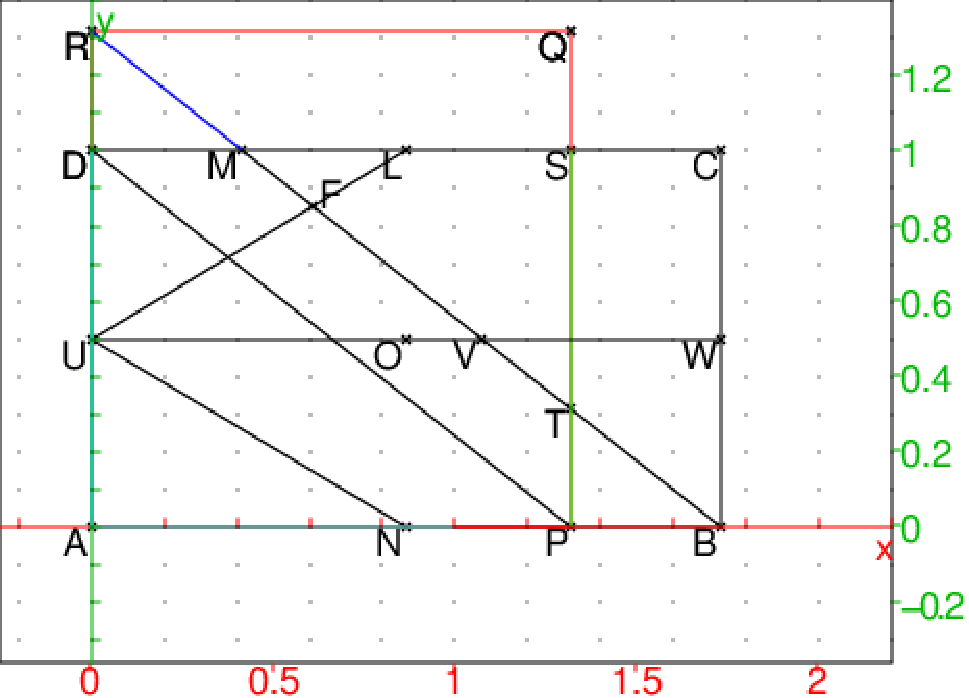
\includegraphics[width=12cm]{puzzleca4}\\
Puis, on tape :
\begin{verbatim}
c:=3/2;
T0:=triangle(A,N,U,affichage=0+rempli);
T1:=polygone(N,P,T,V,U,affichage=1+rempli);
T2:=triangle(T,P,B,affichage=2+rempli);
T3:=triangle(B,W,V,affichage=3+rempli);
T4:=polygone(C,S,L,F,V,W,affichage=4+rempli);
T5:=triangle(U,V,F,affichage=5+rempli);
T6:=triangle(F,L,M,affichage=6+rempli);
T7:=polygone(F,M,D,U,affichage=47+rempli);
affichage(translation(-c*i,T1),1+rempli);
affichage(translation(-sqrt(a*b)-c*i+a*i,T2),2+rempli);
affichage(translation(sqrt(a*b)-b-c*i+(sqrt(a*b)-a)*i,T4),
           4+rempli);
affichage(translation(sqrt(a*b)-b-c*i+(sqrt(a*b)-a)*i,T6),
           6+rempli);
affichage(translation(sqrt(a*b)-b-c*i+(sqrt(a*b)-a)*i,T3),
          3+rempli);
affichage(translation(-c*i,T1),1+rempli);
affichage(translation(-c*i,T0),0+rempli);
affichage(translation(-c*i,T7),47+rempli);
affichage(translation(-c*i,T5),5+rempli);
affichage(translation(3/2-3*c/4*i,T1),1+rempli);
affichage(rotation(N+3/2-3*c/4*i,pi,translation(3/2-3*c/4*i,T0)),
          0+rempli);
affichage(translation(3/2-3*c/4*i,T2),2+rempli);
affichage(translation(3/2-3*c/4*i,T3),3+rempli);
affichage(translation(3/2-3*c/4*i,T4),4+rempli);
affichage(translation(3/2-3*c/4*i,T5),5+rempli);
affichage(rotation(L+3/2-3*c/4*i,pi,
           translation(3/2-3*c/4*i,T6)),6+rempli);
affichage(rotation(L+3/2-3*c/4*i,pi,
           translation(3/2-3*c/4*i,T7)),47+rempli);
\end{verbatim}
On obtient donc 8 pi\`eces :\\
\includegraphics[width=\textwidth]{puzzleca1}
On obtient 6 pi\`eces si on ne fait pas le partage $UW$:\\
\includegraphics[width=\textwidth]{puzzleca2}
\subsection{Un autre d\'ecoupage du rectangle $1*\sqrt3$ avec 6 pi\`eces}
On tape :
\begin{verbatim}
T3:=triangle(sqrt(3),sqrt(sqrt(3)),sqrt(sqrt(3))+i*(sqrt(sqrt(3))-1)):;
P:=inter_unique(droite(y=sqrt(3)/3*x),y=-sqrt(sqrt(3)/3)*(x-sqrt(3)));
T1:=polygone(0,sqrt(sqrt(3)),sqrt(sqrt(3))+i*(sqrt(sqrt(3))-1),P):;
T2:=triangle(sqrt(3),P,sqrt(3)+i):;
T4:=triangle(sqrt(3)+i,P,i+sqrt(3)-sqrt(sqrt(3))):;
T5:=polygone(i,i/2+sqrt(3)/2,P,i+sqrt(3)-sqrt(sqrt(3))):;
T6:=triangle(i,0,i/2+sqrt(3)/2):;
affichage(T1,1+rempli);
affichage(T6,6+rempli);
affichage(T2,2+rempli);
affichage(T3,3+rempli);
affichage(T4,4+rempli);
affichage(T5,5+rempli);
affichage(translation(-2*i+i/2,T1),1+rempli);
affichage(translation(-2*i+i/2,T6),6+rempli);
affichage(translation(-2*i+i/2,T5),5+rempli);
affichage(translation(-3*i-sqrt(3)+sqrt(sqrt(3))+i*sqrt(sqrt(3))+i/2,T2),
           2+rempli);
affichage(translation(-3*i-sqrt(3)+sqrt(sqrt(3))+i*sqrt(sqrt(3))+i/2,T4),
           4+rempli);
affichage(translation(-i-sqrt(sqrt(3))+i/2,T3),3+rempli);
affichage(translation(-i/2+3/2,T1),1+rempli);
affichage(translation(-i/2+3/2,T3),3+rempli);
affichage(translation(-i/2+3/2,T2),2+rempli);
affichage(translation(-3*i/2+3/2,T4),4+rempli);
affichage(translation(-3*i/2+3/2,T5),5+rempli);
affichage(translation(-3/2*i+3/2+sqrt(3),rotation(0,pi/3,T6)),6+rempli);
\end{verbatim}
On obtient 6 pi\`eces :\\
\includegraphics[width=10cm]{carresqrt64}
\subsection{Le carr\'e, le rectangle et le triangle \'equilat\'eral avec 5 
pi\`eces}
Voici les 5 pi\`eces d'un puzzle qui peuvent s'assembler soit en un carr\'e 
soit en un rectangle, soit en 2 paral\'elogramme,  soit en un triangle 
\'equilat\'eral :\\
\includegraphics[width=\textwidth]{puzzlecatri5}\\
On choisit au d\'epart un rectangle de c\^ot\'es de longueur :\\
$\sqrt 6$ et $b=\sqrt 6*sqrt 3/4$.\\
Ce rectangle a la m\^eme surface qu'un triangle \'equilat\'eral de c\^ot\'e 
$\sqrt 6$ et a aussi la m\^eme surface qu'un carr\'e de c\^ot\'e 
$a=\sqrt{3*\sqrt 3/2}$.\\
On tape :
\begin{verbatim}
a:=sqrt(3*sqrt(3)/2);
b:=sqrt(3)/4*sqrt(6);
rectangle(0,sqrt(6),sqrt(3)/4);
A:=point(i*b)+sqrt(6)/4);
B:=point(i*b+3*sqrt(6)/4);
T1:=triangle(0,A,i*b);
T2:=triangle(sqrt(6),B,i*b+sqrt(6));
T3:=triangle(sqrt(6),B,sqrt(6)-a+i*b);
T4:=triangle(a,sqrt(6),a+i*(a-b));
T5:=polygone(A,0,a,a+i*(a-b),i*b+sqrt(6)-a);
\end{verbatim}
On obtient :\\
\includegraphics[width=\textwidth]{puzzlecatri0}\\
On remarque qu'il suffit de faire :\\
\begin{verbatim}
rotation(A,-pi,T1);
rotation(B,pi,T2);
\end{verbatim}
pour obtenir un triangle \'equilat\'eral.
Et on sait facilement transformer ce rectandle en carr\'e avec 
les 3 pi\`eces : (T1+ T5),T4, (T2+T3) selon la m\'ethode 
de la section \ref{sec:carreab}.\\
On tape :
\begin{verbatim}
//le rectangle
affichage(T1,1+rempli);
affichage(T2,2+rempli);
affichage(T3,3+rempli);
affichage(T4,4+rempli);
affichage(T5,5+rempli);
//le triangle equilateral
affichage(translation(2*i,T5),5+rempli);
affichage(translation(2*i,T4),4+rempli);
affichage(translation(2*i,T3),3+rempli);
affichage(translation(2*i,rotation(B,pi,T2)),2+rempli);
affichage(translation(2*i,rotation(A,-pi,T1)),1+rempli);
//le carre
affichage(translation(2*i+3,T5),5+rempli);
affichage(translation(2*i+3,T1),1+rempli);
affichage(translation(2*i+i*(a-b)+3+a-sqrt(6),T2),2+rempli);
affichage(translation(2*i+i*(a-b)+3+a-sqrt(6),T3),3+rempli);
affichage(translation(2*i+i*b+3-a,T4),4+rempli);
//le parallelogramme de base sqrt(6) et de hauteur b
affichage(translation(3.5,T5),5+rempli);
affichage(translation(3.5,T4),4+rempli);
affichage(translation(3.5,T3),3+rempli);
affichage(translation(3.5,T2),2+rempli);
affichage(translation(3.5+sqrt(6),T1),1+rempli);
//l'autre parallelogramme de base a et de hauteur a
affichage(translation(2.5*i+5,T5),5+rempli);
affichage(translation(2.5*i+i*b+5-a,T4),4+rempli);
affichage(translation(2.5*i+5,T1),1+rempli);
affichage(translation(2.5*i-i*b+5+a-sqrt(6),T2),2+rempli);
affichage(translation(2.5*i-i*b+5+a-sqrt(6),T3),3+rempli);
\end{verbatim}
On obtient les 5 quadilat\`eres du d\'ebut :\\
\includegraphics[width=\textwidth]{puzzlecatri5}\\
\subsection{Le carr\'e et le triangle \'equilat\'eral avec 4 pi\`eces}
Voici les 4 pi\`eces d'un puzzle qui peuvent s'assembler soit en un carr\'e 
soit en un triangle \'equilat\'eral :\\
\includegraphics[width=\textwidth]{puzzlecan}\\
Etant donn\'e un carr\'e, trouver la construction de ces pi\`eces et prouvez 
que l'on a  bien obtenu apr\`es r\'eorganisation un triangle \'equilat\'eral.\\
{\bf La solution}\\
\includegraphics[width=\textwidth]{puzzlecatri}\\
Si le carr\'e est de c\^ot\'e {\tt 2a} et le c\^ot\'e du triangle 
\'equilat\'eral est de c\^ot\'e {\tt 2b}.\\ 
On doit avoir (\'egalit\'e des aires):\\
{\tt 4a\verb|^|2=b\verb|^|2*sqrt(3)}
On pose {\tt l:=sqrt(b\verb|^|2-a\verb|^|2)}.\\
On voit que si les figures sont exactes pour obtenir le triangle \`a partir du 
carr\'e de c\^ot\'e {\tt 2a} il faut, sans bouger la pi\`ece bleue, 
faire subir :
\begin{enumerate}
\item \`a la pi\`ece rouge une sym\'etrie par rapport \`a {\tt M:=point(1)} 
\item \`a la pi\`ece jaune une sym\'etrie par rapport \`a {\tt Q:=point(2+i*l)}
\item \`a la pi\`ece verte une translation de vecteur {\tt PP1} si {\tt P1} 
est le sym\'etrique de {\tt P:=point((a-l)*i)}  par rapport \`a {\tt M}.
\end{enumerate}
On doit donc avoir :\\
le c\^ot\'e du triangle \'equilat\'eral $2b$ est \'egal \`a $PR+PN+RN=2PN=2b$,\\
$AM=MB$ donc $M$ est le milieu de $AB$,\\
$DN=NC$ donc $N$ est le milieu de $CD$,\\
$CQ+DP=AP+QB=2a$\\
$RM=RQ=b$\\
$\overbrace{PRM}=\overbrace{MRQ}=\overbrace{QRN}=\pi/3$\\
$4a^2=b^2\sqrt 3$ car le carr\'e et le triangle ont m\^eme surface.\\
Donc $RMQ$ est \'equilat\'eral puisque c'est un triangle isoc\`ele ayant un 
angle de $\pi/3$ et donc 
$\overbrace{RMQ}=\overbrace{PRM}=\overbrace{QRN}=\pi/3$.\\
Puisque on a aussi $\overbrace{MQR}=\overbrace{QRN}=\pi/3$, on en d\'eduit 
que :\\ 
$MQ$ est parall\`ele \`a $PN$ et  $NQ$ est parall\`ele \`a $PM$.\\
les triangles $DNP$ et $BMQ$ sont \'egaux.\\
les triangles $AMP$ et $CNQ$ sont \'egaux.\\ 
le quadrilat\`ere $PMQN$ est un parall\'elogramme.\\
On a donc $AP=QC=2a-l$ et $PD=BQ=l$ et\\ 
aire($PMQN$)=$4a^2-al-(2a-l)a=2a^2=h*\sqrt{a^2+l^2}=hb$ si $h$ est la 
distance entre les parall\`eles  $PN$ et $MQ$.\\
Donc $hb=2a^2=b^2\sqrt 3/2$ et on en d\'eduit $h=b\sqrt 3/2$.\\
R\'eciproquement, si $PD=BQ=l$ et si $RMQ$ est \'equilat\'eral alors :\\
$MQ$ est parall\`ele \`a $PN$ et 
$R$ se trouve sur $PN$ car la hauteur du triangle $RMQ$ qui vaut 
$b\sqrt(3)/2$ est aussi \'egale \`a la distance $h$ entre 
les parall\`eles  $PN$ et $MQ$.
$\overbrace{PRM}=\overbrace{MRQ}=\overbrace{QRN}=\pi/3$\\
Donc 
$\overbrace{PRM}=\overbrace{MQR}=\pi/3\ $ et
$\ \overbrace{QRN}=\overbrace{MQR}=\pi/3$\\
{\bf Autre d\'emonstration}
Si le carr\'e a comme c\^ot\'e $2a$ et le triangle \'equilat\'eral a comme 
c\^ot\'e $2b$ on a :\\
$4a^2=b^2\sqrt 3$ car le carr\'e et le triangle ont m\^eme surface.\\
Posons $l=PD$ on a $b^2=PN^2=l^2+a^2=4a^2/\sqrt(3)$\\
Donc $l^2=a^2(4\sqrt 3/3-1)$\\
Si $PD=BQ=l$ et $AM=MB=DN=NC=a$ on a :\\
$PN=MQ$ et $PM=NQ$ donc la quadrilat\`ere $MPNQ$ est un parall\'elogramme.
$NM$ est parall\'ele \`a $DP$ donc $\overbrace{NPD}=\overbrace{PNM}=\alpha$.
$\sin(\overbrace{NPD})=a/b$ et $\sin(\overbrace{PNM})=h/2a$ donc
$h=\frac{2a^2}{b}=\frac{b\sqrt 3}{2}$.\\
Le point $R$ est donc l'intersection de la m\'ediatrice de $MQ$ avec $PN$.
Le triangle $PQR$ est donc isoc\`ele est sa hauteur issue de $R$ vaut
$h=b\frac{b\sqrt 3}{2}$ donc le triangle $PQR$ est \'equilat\'eral.\\
{\bf Comment construire le point $R$ ?}\\
On a montr\'e que $R$ est le transform\'e de $Q$ dans la rotation de centre $M$
 et d'angle $\pi/3$.\\
On tape pour avoir les pi\`eces du puzzle (on prend pour simplifier $a=1$) :
\begin{verbatim}
l:=sqrt(4*sqrt(3)/3-1);
M:=point(1):;
P:=point(i*(2-l)):;
Q:=point(2+i*l):;
R:=rotation(M,pi/3,Q):;
quadrilatere(M,2,Q,R,affichage=4+rempli); 
quadrilatere(Q,2+2*i,1+2i,R,affichage=3+rempli); 
triangle(P,2i,1+2i,affichage=2+rempli);
quadrilatere(0,M,R,i*(2-l),affichage=1+rempli); 
\end{verbatim}
On obtient :\\
\ \\
\includegraphics[width=8cm]{puzzleca}\\
{\bf Comment construire les pi\`eces \`a partir d'un triangle \'equilat\`eral}\\
Soit un triangle de c\^ot\'e $2b=2$.\\
On tape :\\
\begin{verbatim}
triangle_equilateral(0,2,R));
b:=1;
a2:=b^2*sqrt(3)/4;
l2:=1-a2;
M:=milieu(0,R);
Q:=milieu(2,R);
B:=inter_unique(cercle(M,sqrt(a2)),cercle(Q,sqrt(l2)),point(2));
T4:=polygone(R,M,B,Q);
P:=inter_unique(droite(Q,B),droite(0,2));
T1:=polygone(0,P,B,M);
S:=P+1;
N:=inter_unique(droite(B,Q),perpendiculaire(S,droite(B,Q)));
T3:=polygone(2,Q,N,S);
T2:=triangle(N,P,S);
\end{verbatim}
On obtient :\\
\includegraphics[width=8cm]{puzzlecan0}\\
{\bf Pour animer la figure}\\
On peut animer la figure, soit manuellement avec les curseurs, soit avec la 
commande {\tt animation}.\\
On tape :
\begin{verbatim}
animtri(t1,t2,t3):={
  local L,l,M,P,P1,Q,R;
l:=sqrt(4*sqrt(3)/3-1);
M:=point(1):;
P:=point(i*(2-l)):;
P1:=symetrie(M,P):;
Q:=point(2+i*l):;
R:=rotation(M,pi/3,Q):;
L:=quadrilatere(M,2,Q,R,affichage=4+rempli); 
L:=L,affichage(rotation(M,t1,quadrilatere(0,M,R,i*(2-l))),1+rempli); 
L:=L,affichage(rotation(Q,-t3,quadrilatere(Q,2+2*i,1+2i,R)),3+rempli); 
L:=L,affichage(translation((P1-P)*t2,triangle(i*(2-l),2i,1+2i)),2+rempli);
return L;
}:;
\end{verbatim}
Puis on utilise des param\`etres dans un \'ecran de g\'eom\'etrie, on tape :
\begin{verbatim}
supposons(t1=[0.0,0,3.14,0.1]);
supposons(t3=[0.0,0,3.14,0.1]);
supposons(t2=[0.0,0,1,0.1]);
animtri(t1,t2,t3);
\end{verbatim}
En faisant bouger les curseurs {\tt t1},{\tt t3} et {\tt t2}, on voit les 
pi\`eces du puzzle se d\'eplacer selon les transformations annonc\'ees.\\
Ou bien :\\
On cr\'ee une animation pour voir les d\'eplacements, pour cela on 
cr\'ee les listes que la commande {\tt animation} va utiliser.\\
On tape :\\
\begin{verbatim}
T1:=seq([animtri(t1,0,0)],t1=0..3.14,3.14/10):;
T3:=seq([animtri(3.14,0,t3)],t3=0..3.14,3.14/10):;
T2:=seq([animtri(3.14,t2,3.14)],t2=0..1,0.1):;
T4:=seq([animtri(t1,1,3.14)],t1=3.14..0,3.14/10):;
T6:=seq([animtri(0,1,t3)],t3=3.14..0,3.14/10):;
T5:=seq([animtri(0,t2,0)],t2=1..0,0.1):;
\end{verbatim}
Puis on tape :\\
{\tt animation(T1,T3,T2,T4,T6,T5)}
\section{La quadrature d'un dod\'eca\`edre}
\subsection{Le dod\'eca\`edre}
On d\'efinit les points utiles.\\
On tape :
\begin{verbatim}
LP:=[point(exp(k*i*pi/6))$(k=0..11)]:;
[A,B,C,D,E,F,G,H,I,J,K,L]:=LP;
polygone(LP);
triangle_equilateral(A,B,M);
triangle_equilateral(J,I,N);
triangle_equilateral(F,E,P);
O:=isobarycentre(F,M,I);
\end{verbatim}
On obtient :\\
\includegraphics[width=\textwidth]{carredode}
{\bf Exercice}\\
On trace le dod\'ecacone $ABCDEFGHIJKL$ inscrit dans un cercle de rayon 1 
unit\'e et le triangle \'equilat\`eral $ABM$ comme ci-dessus, puis on trace 
les 4 segments : cela d\'etermine 6 r\'egions :\\
\begin{verbatim}
segment(A,I);
segment(B,F);
segment(A,F);
segment(B,I);
\end{verbatim}
\includegraphics[width=\textwidth]{carredode0}\\
Montrer que $AF$ et $BI$ se coupent en $M$ sommet du triangle \'equilat\`eral 
$ABM$.\\
Montrer que le triangle $FMI$ est \'equilat\'eral.\\
Calculer les angles des triangles $MBF$ et $MAI$.\\
Calculer les angles des triangles $AIL$ et $BCF$.
Montrer que $AI=BF=\sqrt 3$\\
\subsection{Le dod\'eca\`edre et le carr\'e}
{\bf Exercice}\\
Soit un dod\'eca\`edre inscrit dans un cercle de rayon 1 unit\'e.\\
Calculer son aire.\\
Calculer le c\^ot\'e du carr\'e qui a la m\^eme aire que ce dod\'ecagone.\\
{\bf R\'eponse}\\
Aire du dod\'eca\`edre= $12\sin(2*pi/12)/2=6\sin(pi/6)=3$ unit\'e*unit\'e.\\
Le c\^ot\'e du carr\'e qui a la m\^eme aire est donc : $\sqrt 3$ unit\'es.\\
{\bf Le d\'ecoupage}\\
On d\'ecoupe le dod\'eca\`edre en 6 morceaux, puis on forme un carr\'e avec 
ces 6 morceaux.\\
D'apr\`es ce qui pr\'ec\`ede $AI$ et $BF$ ont pour longueur le c\^ot\'e du 
carr\'e cherch\'e.\\
On tape :
\begin{verbatim}
P1:=polygone(A,I,J,K,L):;
affichage(P1,1+rempli);
P2:=polygone(B,C,D,E,F):;
affichage(P2,2+rempli);
P3:=triangle_equilateral(A,B,M):;
affichage(P3,3+rempli);
P4:=triangle(M,I,A):;
affichage(P4,4+rempli);
P5:=triangle(M,F,B):;
affichage(P5,5+rempli);
P6:=polygone(F,G,H,I,M):;
affichage(P6,6+rempli);
O:=isobarycentre(F,M,I):;
affichage(translation(3,P6),6+rempli);
affichage(translation(3,rotation(O,2*pi/3,P4)),4+rempli)
affichage(translation(3,rotation(O,-2*pi/3,P5)),5+rempli);
affichage(translation(3-A+H,P3),3+rempli);
triangle_equilateral(J,I,N):;
affichage(translation(3,rotation(
                  isobarycentre(I,J,N),pi/2+pi/6,P1)),1+rempli);
triangle_equilateral(F,E,P):;
affichage(translation(3,rotation(
                  isobarycentre(F,E,P),-pi/2-pi/6,P2)),2+rempli);
\end{verbatim}
On obtient :\\
\includegraphics[width=\textwidth]{carredode1}
\subsection{Pour animer la figure}
On peut animer la figure, manuellement avec les curseurs.\\
On tape :
\begin{verbatim}
affichage(P6,6+rempli);
supposons(t1=[1.0,0,1,0.1]);
affichage(rotation(isobarycentre(I,J,N),-t1*4*pi/3,P1),1+rempli) ;
supposons(t2=[1.0,0,1,0.1]);
affichage(rotation(isobarycentre(F,E,P),(t2)*4*pi/3,P2),2+rempli);
supposons(t3=[1.0,0,1,0.1]);
affichage(translation(t3*(H-A),P3),3+rempli);
supposons(t4=[1.0,0,1,0.1]);
affichage(rotation(O,t4*2*pi/3,P4),4+rempli);
supposons(t5=[1.0,0,1,0.1]);
affichage(rotation(O,-t5*2*pi/3,P5),5+rempli);
O;
N;
P;
\end{verbatim}
On peut aussi animer la figure avec la commande {\tt animation}.\\
On tape (attention les variables P1,..P6,A,H,E,F,I,J,n,P sont globales) :
\begin{verbatim}
animdode(t1,t2,t3,t4,t5):={
local L; 
L:=NULL;
L:=L,affichage(P6,6+rempli);;
L:=L,affichage(rotation(isobarycentre(I,J,N),-t1*4*pi/3.,P1),
                                                  1+rempli);
L:=L,affichage(rotation(isobarycentre(F,E,P),(t2)*4*pi/3.,P2),
                                                  2+rempli);
L:=L,affichage(translation(t3*(H-A),P3),3+rempli);
L:=L,affichage(rotation(O,t4*2*pi/3,P4),4+rempli);
L:=L,affichage(rotation(O,-t5*2*pi/3,P5),5+rempli);
return L;
}:;
\end{verbatim}
Puis si on utilise un seul param\`etre (tout bouge en m\^eme temps !!!):\\
{\tt K1:=seq([animdode(t1,t1,t1,t1,t1)],t1=0.0..1.0,0.1):;}\\
{\tt K2:=seq([animdode(t1,t1,t1,t1,t1)],t1=1.0..0.0,0.1):;}\\
{\tt animation(K1,K2)}\\
Ou bien si on utilise 5 param\`etres :
\begin{verbatim}
T1:=seq([animdode(t1,0,0,0,0)],t1=0.0..1.0,0.1):;
T2:=seq([animdode(1,t2,0,0,0)],t2=0.0..1.0,0.1):;
T3:=seq([animdode(1,1,t3,0,0)],t3=0.0..1.0,0.1):;
T4:=seq([animdode(1,1,1,t4,0)],t4=0.0..1.0,0.1):;
T5:=seq([animdode(1,1,1,1,t5)],t5=0.0..1.0,0.1):;
T6:=seq([animdode(1,1,1,1,t5)],t5=1.0..0.0,0.1):;
T7:=seq([animdode(1,1,1,t4,0)],t4=1.0..0.0,0.1):;
T8:=seq([animdode(1,1,t3,0,0)],t3=1.0..0.0,0.1):;
T9:=seq([animdode(1,t2,0,0,0)],t2=1.0..0.0,0.1):;
T0:=seq([animdode(t1,0,0,0,0)],t1=1.0..0.0,0.1):;
\end{verbatim}
Puis on tape :\\
{\tt animation(T1,T2,T3,T4,T5,T6,T7,T8,T9,T0)}\\
Ou encore si on n'utilise que 4  param\`etres (en \'echangeant la pi\`ece bleue 
avec la pi\`ece violette \`a l'aide d'un seul param\`etre).\\
\begin{verbatim}
Q1:=seq([animdode(t1,0,0,0,0)],t1=0.0..1.0,0.1):;
Q2:=seq([animdode(1,t2,0,0,0)],t2=0.0..1.0,0.1):;
Q3:=seq([animdode(1,1,t3,0,0)],t3=0.0..1.0,0.1):;
Q4:=seq([animdode(1,1,1,t4,t4)],t4=0.0..1.0,0.1):;
Q7:=seq([animdode(1,1,1,t4,t4)],t4=1.0..0.0,0.1):;
Q8:=seq([animdode(1,1,t3,0,0)],t3=1.0..0.0,0.1):;
Q9:=seq([animdode(1,t2,0,0,0)],t2=1.0..0.0,0.1):;
Q0:=seq([animdode(t1,0,0,0,0)],t1=1.0..0.0,0.1):;
\end{verbatim}
Puis on tape :\\
{\tt animation(Q1,Q2,Q3,Q4,Q7,Q8,Q9,Q0)}
\section{L'hexagone, le rectangle et le carr\'e}
On consid\`ere un rectangle de c\^ot\'es 3 et $\sqrt 3/2$.\\
On transforme facilement ce rectangle en un hexagone de c\^ot\'e 1 avec 3 
pi\`eces.\\
On sait transformer ce rectangle en un carr\'e avec 3 pi\`eces selon la 
m\'ethode vue en section \ref{sec:carreab}.\\  
Avec 6 pi\`eces on peut passer de l'hexagone au carr\'e via le rectangle.\\
On tape :
\begin{verbatim}
a:=sqrt(3*sqrt(3)/2);
b:=sqrt(3)/2;
d:=droite(3,3-a+i*b):;
Q:=inter_unique(droite(y=b),d):;
R:=inter_unique(droite(x=a),d):;
P1:=polygone(R,Q,1/2+i*b,1,a):;
affichage(P1,1+rempli);
P2:=polygone(R,a,2,S):;
affichage(P2,2+rempli);
P3:=polygone(Q,S,5/2+i*b):;
affichage(P3,3+rempli);
P4:=triangle(S,2,3):;
affichage(P4,4+rempli);
P5:=polygone(S,3,3+i*b,5/2+i*b):;
affichage(P5,5+rempli);
P6:=polygone(i*b,0,1,1/2+i*b):;
affichage(P6,6+rempli);
affichage(translation(i+2,P1),1+rempli);
affichage(translation(i+2,P2),2+rempli);
affichage(translation(i+2,P3),3+rempli);
affichage(translation(i+i*b-3/2+2,P4),4+rempli);
affichage(translation(i+i*b-3/2+2,P5),5+rempli);
affichage(translation(i+i*b+3/2+2,P6),6+rempli);
affichage(translation(i,P1),1+rempli);
affichage(translation(i,P6),6+rempli);
affichage(translation(i+i*b-a,P2),2+rempli);
affichage(translation(i+i*b-a,P4),4+rempli);
affichage(translation(i+i*(a-b)-3+a,P3),3+rempli);
affichage(translation(i+i*(a-b)-3+a,P5),5+rempli);
\end{verbatim}
On obtient :\\
\includegraphics[width=\textwidth]{carrehexa}
\chapter{Pour s'amuser avec les probabilit\'es}
\section{Les anniversaires de 3 personnes}
Trois amis sont n\`es une m\^eme ann\`ee de 365 jours.\\
On suppose que les dates de naissance sont \'equiprobables.\\
Quelles sont les probabilit\'es pour que :

1/ Ils soient n\'es le m\^eme jour,

2/ Deux d'entre eux seulement soient n\'es le m\^eme jour,

3/ Ils soient n\'es a des dates diff\'erentes,

4/ Quelle relation v\'erifie ces trois r\'eponses ?\\

{\bf Solution}\\
On donne un num\'ero aux amis, i.e. on les ordonne.\\
Soit $\Omega$ l'univers ensemble de triplets de nombres allant de 1 \`a 365.
Il y a $365^3$ triplets possibles, donc   $card(\Omega)=365^3$.

1/ Soit $A$ l'\'ev\'enement "Ils sont tous les trois n\'es le m\^eme jour". cela signifie que 
$A$ est compos\'e de tripl\'es form\'es par 3 nombres \'egaux donc, 
$card(A)=365$. \\
Donc, $p(A)=\frac{365}{365^3}=\frac{1}{365^2}\simeq 7.5e-06$.

2/ Soit $B$ l'\'ev\'enement "Deux seulement sont n\'es le m\^eme jour".
$B$ est compos\'e de tripl\'es form\'es par 2 nombres \'egaux et diff\'erents 
du 3-i\`eme. Il  y a trois possibilit\'es (les deux premiers  ou les deux 
derniers ou le premier et le troisi\`eme)  ont le m\^eme anniversaire donc,
comme il y a $365*364$ couples de nombres diff\'erents, $card(B)=3*365*364$.\\
Donc, $p(B)=\frac{3*365*364}{365^3}=\frac{3*364}{365^2}\simeq 0.0082$.

3/ Soit $C$ l'\'ev\'enement "Ils sont n\'es a des dates diff\'erentes".
$C$ est compos\'e de tripl\'es form\'es par 3 nombres diff\'erents donc,
comme il y a $365*364*363$ triplets form\'es de 3 nombres diff\'erents, on a
$card(C)=365*364*363$.\\
Donc, $p(C)=\frac{365*364*363}{365^3}=\frac{364*363}{365^2}\simeq 0.99$.

4/ On doit avoir $p(A)+p(B)+p(C)=1$ puisque $A,B,C$ forment une partition de 
 $\Omega$. on a :\\
$1+3*364+364*363=1+364*366=1+(365-1)(365+1)=365^2$\\
donc on a bien : $p(A)+p(B)+p(C)=1$.\\
\section{Les anniversaires de {\tt n} personnes}
Dans une assembl\'ee de {\tt n} personnes, toutes sont n\`ees une ann\`ee de 
365 jours.\\
On suppose que les dates de naissance sont \'equiprobables.\\
On note {\tt p(n)} la probabilit\'e pour que 2 personnes au moins aient leur 
anniversaire le m\^eme jour.

1/ Calculer {\tt p(3)},

2/ Donner la formule permettant de calculer {\tt p(n)},

3/ D\'eterminer une valeur approch\'ee de 
{\tt p(20)}, {\tt p(30)} et {\tt p(367)},

4/ D\'eterminer le nombre {\tt n} pour que l'on ait 
${\tt p(n)\geq \frac{1}{2}}$.\\

{\bf Solution}\\
On donne un num\'ero aux personnes de l'assembl\'ee, i.e. on les ordonne.\\
Soit $\Omega$ l'univers ensemble des {\tt n}-uplets de nombres entiers de 1 
\`a 365.\\ 
Il y a ${\tt 365^n}$ triplets possibles, donc ${\tt card(\Omega)=365^n}$.

1/ D'apr\`es l'exercice pr\'ec\'edent, {\tt p(3)}=$p(A)+p(B)=\frac{1+3*364}{365^2}\simeq 0.0082$.

2/ On va tout d'abord chercher la probabilit\'e de l'\'ev\'enement contraire :
soit $D_n$ l'\'ev\'enement "Les {\tt n} personnes ont leurs anniversaires 
a des dates toutes diff\'erentes".

Il y a ${\tt 365*364*...*365-n+1}$ triplets form\'es de nombres diff\'erents 
deux \`a deux, donc $card(D_n)=365*364*...365-n+1=\frac{365!}{(365-n)!}$.\\ 
Donc $\displaystyle p(D_n)=\frac{365!}{(365-n)!*365^n}=\frac{364!}{(365-n)!*365^{n-1}}$,\\
et donc $\displaystyle p(n)=1-p(D_n)=\frac{(365-n)!*365^n-365!}{(365-n)!*365^n}=\frac{(365-n)!*365^{n-1}-364!}{(365-n)!*365^{n-1}}$.\\
Avec {\tt Xcas} on peut d\'efinir {\tt p(n)} on tape :\\
{\tt p(n):=1-factorial(364)/(factorial(365-n)*365\verb|^|(n-1))}

3/ Calculons avec {\tt Xcas}, on tape :\\
{\tt evalf(perm(365,19)/365\verb|^|19)}\\
 On obtient :\\
{\tt 0.588561616419}\\
donc $p(D_{20})\simeq 0.588561616419$ et \\
{\tt p(20)}$\simeq (1-0.588561616419) \simeq ${\tt 0.411438383581}\\
Ou on tape :\\
{\tt evalf(p(20))}\\
On obtient :\\
{\tt 0.411438383581}\\
On tape :\\
{\tt evalf(perm(364,22)/365\verb|^|22)}\\
On obtient :\\
{\tt 0.492702765676}\\
donc $p(D_{23})\simeq 0.492702765676$ et\\ 
{\tt p(25)}$\simeq (1-0.492702765676) \simeq ${\tt0.507297234324}\\
Ou on tape :\\
{\tt evalf(p(23))}\\
On obtient :\\
{\tt 0.507297234324}\\
On tape :\\
{\tt evalf(perm(365,29)/365\verb|^|29)}\\
On obtient :\\
{\tt 0.293683757281}\\
donc $p(D_{30})\simeq 0.293683757281$ et\\ 
{\tt p(30)}$\simeq (1-0.293683757281) \simeq ${\tt0.706316242719}\\
Ou on tape :\\
{\tt evalf(p(30))}\\
On obtient :\\
{\tt 0.706316242719}\\
Ce qui veut dire que dans une assembl\'ee de 
20 personnes il y a 4 chances sur 10 pour que 2 personnes aient le m\^eme 
anniversaire, que dans une assembl\'ee de 23 personnes il y a 1 chance sur 
2 pour que 2 personnes aient le m\^eme anniversaire et que dans une 
assembl\'ee de 30 personnes il y a 7 chances sur 
10 pour que 2 personnes aient le m\^eme anniversaire !!!!\\
Pour calculer $p(367)$, on n'a pas besoin de {\tt Xcas} car :\\
 $p(367)=1$ puisqu'il n'y a que 365 dates possibles (ou 366 ...) parmi
les 367 personnes et donc deux  personnes au moins ont forc\'ement le m\^eme 
anniversaire.

4/ On va utiliser le tableur pour chercher $p(20)..p(30)$, pour cela on tape 
dans {\tt A0}..{\tt A10} les valeurs de $p(D_ {20})..p(D_ {30})$ :\\
 {\tt =evalf(perm(365,20+Row())/365\verb|^|(20+Row()))}\\
et dans {\tt B0} ..{\tt B10} les valeurs de $p(20)..p(30)$ :\\
 {\tt =1-A0}\\
Puis, on remplit les colonnes {\tt A} et {\tt B} avec ces formules \`a l'aide
du bouton {\tt remplir} (option {\tt vers le bas}).\\
On rapelle que pour avoir la valeur d'une cellule dans la ligne de commande,
on doit appuyer sur le bouton {\tt eval}.\\
On obtient :\\
{\tt B2=0.475695307663} et {\tt B3=0.507297234324}\\
donc $n=23$ car on a :\\
$p(23)=0.507297234324>0.5$ et\\
pour $n=22$ $p(22)=0.475695307663<0.5$.\\
On peut aussi taper dans {\tt C0} :\\
{\tt =20+count\_inf(0.5,B0:B10)} \\
car on sait que $20<n<30$  et que {\tt coun\_inf(0.5,B0:B10)} est la fonction 
qui compte le nombre d'\'el\'ements stricrement inf\'erieurs \`a 0.5 dans la 
colonne {\tt B} (de {\tt B0} \`a {\tt B10}).\\
 On a mis 20 car il a {\tt 19+count\_inf(0.5,B0:B10)} valeurs stricrement 
inf\'erieures \`a 0.5 et donc {\tt 20+count\_inf(0.5,B0:B10)} est la 
premi\`ere valeur sup\'erieure ou \'egale  \`a 0.5.\\
On obtient dans {\tt C0} :\\
{\tt 23}\\
On remarqera que :\\
{\tt B21=0.903151611482}\\
Ce qui veut dire que dans une assembl\'ee de 41 personnes il y a 9 chances sur 
10 pour que 2 personnes aient le m\^eme anniversaire !!!!

5/ On peut dessiner l'\'evolution des {\tt p(n)} en fonction de {\tt n} lorsque
{\tt n} varie entre 20 et 50.
Il suffit poir cela de rajouter une colonne entre 
{\tt A} et {\tt B} on met {\tt B0}  en surbrillance et on appuie sur 
{\tt c+}. La colonne {\tt B} devient {\tt C}, et une colonne {\tt B} est 
cr\'e\'ee. \\
On tape alors {\tt 0} dans {\tt B0}, puis dans {\tt B1} on met
{\tt =B0+1} puis on remplit la colonne {\tt B} avec cette formule.\\
Il suffit maintenant de mettre en surbrillance {\tt B0:C30} puis d'ouvrir le 
menu {\tt 2d} et de choisir {\tt Scatterplot} pour voir les diff\'erents 
points dans l'\'ecran de g\'eom\'etrie (changer la configuration du 
graphique pour voir tous les points).
\section{Les 4 d\'es du jeu de Win}\label{sec:win}
On consid\`ere les 4 d\'es suivants :
\begin{itemize}
\item les faces du d\'e {\tt A} ont comme points : {\tt 0,0,4,4,4,4}, 
\item les faces du d\'e {\tt B} ont comme points : {\tt 1,1,1,5,5,5},
\item les faces du d\'e {\tt C} ont comme points : {\tt 2,2,2,2,6,6},
\item les faces du d\'e {\tt D} ont comme points : {\tt 3,3,3,3,3,3},
\end{itemize}
La partie se compose de 12 lancers.\\Pour une partie, chacun des joueurs 
choisit un d\'e. \`A chaque lancer, celui
qui a le meilleur score marque 1 point. La partie se compose de 12 lancers.\\
On veut simuler ce jeu pour que l'on puisse jouer contre l'ordinateur.
L'ordinateur tire au hasard un d\'e, vous donne son choix, puis vous
choisisez un parmi les 3 d\'es qui restent. Puis vous jouez....\\
Quel d\'e faut-il choisir pour gagner contre l'ordinateur ?
\ \\
On num\'erote les faces de chaque d\'e : par exemple, par ordre croissant des 
points des faces, ainsi pour le  d\'e {\tt A} les faces 0,1 ont comme 
points 0 et les faces 2,3,4,5 ont comme points 4.  
Pour jouer avec un d\'e, on tire au hasard un nombre entier entre 0 et 
5 ({\tt rand(6)}) pour voir sur quelle face tombe le d\'e, puis on regarde le 
nombre de points de cette face. Ce nombre d\'epend du d\'e choisi.\\
On \'ecrit donc une fonction qui renvoie pour chaque d\'e la valeur de
la face {\tt n} du d\'e. 
\begin{verbatim}
rande(des,n):={
if (des=="A"){if (n==0 or n==1) return 0 ;
                             else return 4;};
if (des=="B"){if (n==0 or n==1 or n==2) return 1; 
                             else return 5;};
if (des=="C"){if (n==4 or n==5) return 6;
                             else return 2;};
return 3;
}:;
\end{verbatim}
Puis on \'ecrit le programme qui correspond a une partie (12 lancers pour 
chacun) et qui renvoie la liste des scores (ordinateur,joueur).
\begin{verbatim}
jeuwin0():={
local deo,dem,po,pm,scoro,j;
deo:=char(rand(4)+65);
print("j'ai choisi le de "+ deo);
repeter saisir_chaine("votre choix",dem);
jusqua dem!=deo;
scoro:=0;
for (j:=0;j<12;j++){
po:=rande(deo,rand(6));
pm:=rande(dem,rand(6));
print(po,pm);
if (po>pm) scoro:=scoro+1;
}
return [scoro,12-scoro];
}
:;
\end{verbatim}
On peut aussi utiliser les listes A,B,C,D pour representer chaque d\'e, et le 
programme devient beaucoup plus simple (on n'a pas besoin de la fonction
{\tt rande} !!!!) mais il faut transformer le caract\`ere contenu dans 
{\tt deo} (par ex {\tt "A"}) en {\tt expr(deo)} (par ex en la valeur de la 
variable {\tt A}). Pour {\tt dem} on ne saisit plus une chaine mais directement
le nom d'une variable avec {\tt saisir(dem)} au lieu de {\tt saisir\_chaine(dem)}.
\begin{verbatim}
jeuwin():={
local deo,dem,po,pm,scoro,j,A,B,C,D;
deo:=char(rand(4)+65);
print("j'ai choisi le de "+ deo);
A:=[0,0,4,4,4,4];
B:=[1,1,1,5,5,5];
C:=[2,2,2,2,6,6];
D:=[3,3,3,3,3,3];
deo:=expr(deo);
repeter saisir("votre choix",dem);
jusqua dem!=deo;
scoro:=0;
for (j:=0;j<12;j++){
po:=deo[rand(6)];
pm:=dem[rand(6)];
print(po,pm);
if (po>pm) scoro:=scoro+1;
}
return [scoro,12-scoro];
}
:;
\end{verbatim}
On peut ensuite faire plusieurs parties. On tape :\\
{\tt score:=[0,0];}\\
puis par exemple\\
{\tt score:=score+jewin()}\\
plusieurs fois et on obtient les scores cumul\'es.

Pour savoir quel d\'e il faut choisir, on cherche la probabilit\'e
que l'ordinateur gagne selon les diff\'erents choix :
\begin{enumerate}
\item l'ordinateur a choisi le d\'e {\tt A},
\begin{itemize}
\item si vous choisissez le d\'e {\tt B},\\
L'ordinateur gagne si le d\'e {\tt A} fait quatre et le d\'e {\tt B} fait un,
donc 
$$P(nA>nB)=(4/6)*(3/6)=1/3$$
\item si vous choisissez le d\'e {\tt C},\\
L'ordinateur gagne si le d\'e {\tt A} fait quatre et le d\'e {\tt C} fait deux,
donc 
$$P(nA>nC)=(4/6)*(4/6)=4/9$$ 
\item si vous choisissez le d\'e {\tt D},\\
L'ordinateur gagne si le d\'e {\tt A} fait quatre, donc 
$$P(nA>nD)=(4/6)=2/3$$ 
\end{itemize}
Il faut donc choisir le d\'e {\tt B} pour gagner avec une probabilit\'e de 2/3.
\item l'ordinateur a choisi le d\'e {\tt B},
\begin{itemize}
\item si vous choisissez le d\'e {\tt C},\\
L'ordinateur gagne si le d\'e {\tt B} fait cinq et le d\'e {\tt C} fait deux,
donc 
$$P(nB>nC)=(3/6)*(4/6)=1/3$$ 
\item si vous choisissez le d\'e {\tt D},\\
L'ordinateur gagne si le d\'e {\tt B} fait cinq,
donc 
$$P(nB>nD)=(3/6)=1/2$$ 
\item si vous choisissez le d\'e {\tt A},\\
cas d\'ej\`a vu :
$P(nB>nA)=1-P(nA>nB)=2/3$
\end{itemize}
Il faut donc choisir le d\'e {\tt C} pour gagner avec une probabilit\'e de 2/3.
\item l'ordinateur a choisi le d\'e {\tt C},
\begin{itemize}
\item si vous choisissez le d\'e {\tt D},\\
L'ordinateur gagne si le d\'e {\tt C} fait six,
donc 
$$P(nC>nD)=(2/6)=1/3 $$
\item si vous choisissez le d\'e {\tt B},\\
cas d\'ej\`a vu :
$ P(nC>nB)=1-P(nB>nC)=2/3$
\item si vous choisissez le d\'e {\tt A},\\
cas d\'ej\`a vu :
$ P(nC>nA)=1-P(nA>nC)=5/9$
\end{itemize}
Il faut donc choisir le d\'e {\tt D} pour gagner avec une probabilit\'e de 2/3.
\item l'ordinateur a choisi le d\'e {\tt D},
\begin{itemize}
\item si vous choisissez le d\'e {\tt A},\\
cas d\'ej\`a vu : $P(nD>nA)=1-P(nA>nD)=1/3$ 
\item si vous choisissez le d\'e {\tt B},\\
cas d\'ej\`a vu : $P(nD>nB)=1-P(nB>nD)=1/2$
\item si vous choisissez le d\'e {\tt C},\\
cas d\'ej\`a vu : $P(nD>nC)=1-P(nC>nD)=2/3$
\end{itemize}
Il faut donc choisir le d\'e {\tt A} pour gagner avec une probabilit\'e de 2/3.
\end{enumerate}
{\bf Remarque}\\
La relation "le d\'e $N_1$ gagne le d\'e $N_2$" n'est pas transitive, 
en effet:\\
le d\'e {\tt B} gagne le d\'e {\tt A},\\
le d\'e {\tt C} gagne le d\'e {\tt B},\\
le d\'e {\tt D} gagne le d\'e {\tt C},\\
le d\'e {\tt A} gagne le d\'e {\tt D},\\
De plus, le jeu est trompeur car le choix ne depend pas du score moyen de 
chaque d\'e, en effet :\\ 
le d\'e {\tt A} fait en moyenne un score de 8/3,\\
le d\'e {\tt B} fait en moyenne un score de 3,\\
le d\'e {\tt C} fait en moyenne un score de 10/3,\\
le d\'e {\tt D} fait en moyenne un score de 3 et pourtant le d\'e {\tt D}
l'emporte sur le d\'e {\tt C} de moyenne 10/3 mais il perd contre le d\'e 
{\tt A} qui n'a qu'une moyenne de 8/3 !


\section{Des calculs de moyenne}
\subsection{Nombre d'enfants moyen par famille}
Dans un pays, le roi a d\'ecid\'e que les familles de ses sujets doivent avoir
des enfants jusqu'\`a ce qu'elles aient un gar\c{c}on.\\
Quelle est le nombre d'enfants moyen par famille ?

Si $X$ est la variable al\'eatoire \'egale au nombre d'enfants dans une 
famille, on a :
\begin{itemize}
\item $\displaystyle P(X=1)=\frac{1}{2}$
\item $\displaystyle P(X=2)=\frac{1}{2^2}$
\item $\displaystyle P(X=3)=\frac{1}{2^3}$
\item ....
\item $\displaystyle P(X=k)=\frac{1}{2^k}$
\end{itemize}
Donc $\displaystyle E(X)=\sum_{k=1}^{+\infty} k*\frac{1}{2^k}$\\
On tape :\\
{\tt sum(k/2\verb|^|k,k,1,+infinity)}\\
On obtient :\\
{\tt 2}\\
Donc le nombre moyen d'enfants est 2....On aurait pu s'en douter car dans 
chaque famille il n'y a qu'un seul gar\c{c}on et comme en moyenne il nait 
autant de filles que de gar\c{c}ons, il y aura en moyenne autant de filles que 
de gar\c{c}ons, soit 2 enfants en moyenne dans chaque famille.

\subsection{Nombres triangulaires al\'eatoires}
On tire au hasard des nombres entre 1 et $n$ jusqu'\`a obtenir 1. Le 
r\'esultat est alors la somme des nombres obtenus. Quel est la moyenne des 
r\'esultats obtenus ?

\subsubsection{La solution math\'ematique}
Supposons pour commencer $n=2$\\
Les r\'esultats peuvent \^etre : $R=1,3,5....2p+1....$\\
On a :\\
$\displaystyle P(R_2=1)=\frac{1}{2}$,\\
$\displaystyle P(R_2=3)=\frac{1}{2^2}$\\
....
$\displaystyle P(R_2=2p+1)=\frac{1}{2^{p+1}}$\\
Donc :\\
$\displaystyle E(R_2)=\sum_{p=0}^{+\infty} (2p+1)\frac{1}{2^{p+1}}$\\
On tape :\\
{\tt sum((2k+1)/2\verb|^|(k+1),k,0,+infinity)}\\
On obtient :\\
{\tt 3}\\
La moyenne de $R_2$ vaut donc 1+2=3.\\

Peut-on g\'en\'eraliser ?\\
Dans le cas g\'en\'eral, on tire au hasard des nombres entre 1 et $n$ jusqu'\`a
obtenir 1. La moyenne des sommes des nombres tir\'es vaut-elle 
$1+2+...+n=n(n+1)/2$ ?\\
Soit $X_n$ la variable al\'eatoire \'egale au nombre de tirages parmi 
$1...n$ qu'il faut effectuer pour obtenir 1.\\
On a :\\
$\displaystyle P(X_n=1)=\frac{1}{n}$,\\
$\displaystyle P(X_n=2)=\frac{1}{n^2}$ et les r\'esultats obtenus peuvent 
\^etre : \\
$2+1=3,3+1=4,...,n+1$ qui est une liste $L_2$ de taille $n-1$ et de somme :\\
$2+3+...n+n-1=(n-1)(n+3)/2$
\\
$\displaystyle P(X_n=3)=\frac{1}{n^3}$ et les r\'esultats obtenus peuvent 
\^etre : \\
$2+2+1=5,2+3+1=6,3+2+1=6,...n+n+1$ qui est une liste $L_3$ de taille 
$(n-1)^2$\\
Que vaut la somme de cette liste ?\\
Chaque terme est la somme de 2 termes et de 1 : dans ces sommes chaque nombre 
(2,3,...n) apparaissent autant de fois donc il y a $2(n-1)^2/(n-1)=2n-2$ fois 2,
$2n-2$ fois 3...$2n-2$ fois $n$ et $(n-1)^2$ fois 1. La somme cette liste vaut 
donc :\\
$(n-1)^2+(2n-2)(2+3+...+n)=(n-1)^2+(n-1)^2(n+2)=(n-1)^2(n+3)$.\\
......
$\displaystyle P(X_n=p)=\frac{1}{n^p}$ et les r\'esultats obtenus peuvent 
\^etre : $2+...+2+1=2p-1,2+...+3+1=2p,3+2+...+2+1=2p,...$ (liste $L_p$ de 
taille $(n-1)^{p-1}$)\\
Que vaut la somme de cette liste ?\\
Cette somme est compos\'ee de $p*(n-1)^{p-1}$ termes.\\
Cette somme est la somme :\\
de $(n-1)^{p-1}$ fois 1,\\
de $(p-1)(n-1)^{p-2}$ fois 2\\
....\\
de $(p-1)(n-1)^{p-2}$ fois $n$\\
 donc elle vaut :\\
$(n-1)^{p-1}+(p-1)(n-1)^{p-2}(2+3+...+n)=$\\
$(n-1)^{p-1}+(n-1)^{p-1}(p-1)(n+2)/2=(n-1)^{p-1}(1+(p-1)(n+2)/2)=$\\
$(n-1)^{p-1}((p(n+2)-n)/2)$.\\
Donc :\\
$E(R_n)=\sum_{p=1}^{+\infty}\frac{1}{n^p}(n-1)^{p-1}(p(n+2)-n)/2$\\
On tape :\\
{\tt sum((n-1)\verb|^|(p-1)/n\verb|^|p*(p*(n+2)-n)/2 ,p,1,+infinity)}\\
On obtient :\\
{\tt (n\verb|^|2+n)/2}\\
Donc la moyenne de $R_n$ est \'egale \`a $1+2+...n$
\subsubsection{La mod\'elisation avec {\tt Xcas}}
On tape le programme {\tt trialea(r,q,p)} qui tire au hasard des nombres entre
1 et $r$. On fait $p$ fois des \'echantillons de taille $q$, et on dessine
les r\'esultats interm\'ediaires obtenus :
{\tt l} contient les sommes cumul\'ees des r\'esultats (ici une somme) c'est 
\`a dire la 
somme d'un \'echantillon de taille {\tt n=k+1+j*q} avec  {\tt k=0..q-1} et
{\tt j=0..p-1}. Dans {\tt Ldiv} on met {\tt evalf(l/n)}  lorsque 
{\tt n=q,2*q...p*q} 
\begin{verbatim}
trialea(r,q,p):={
  local j,k,l,n,LdivN,alea;
  LdivN:=NULL;
  l:=0;
  n:=0;
  for (j:=0;j<p;j++){
    for (k:=0;k<q;k++){
      alea:=(rand(r)+1);
      while (alea!=1){
        l:=l+alea;
        alea:=(rand(r)+1);
      }
      l:=l+1;
      n:=n+1;
    }
    LdivN:=LdivN,evalf(l/n);
  }
  return LdivN;
}:;
\end{verbatim}
On tape :\\
{\tt L10:=trialea(10,100,10000);}\\
{\tt plotlist(L10)}\\
On obtient :\\
\ \\
 \includegraphics[width=\textwidth]{trialea}
\subsection{Factorielles al\'eatoires}
On tire au hasard des nombres entre 1 et $n$ jusqu'\`a obtenir 1. Le 
r\'esultat est alors le produits des nombres obtenus. Quel est la moyenne des 
r\'esultats obtenus ?

\subsubsection{La solution math\'ematique}
Cela ressemble \`a l'exercice pr\'ec\'edent.....\\
Supposons pour commencer $n=2$.\\
Les r\'esultats peuvent \^etre : $R=1,2,4....2^p...$\\
On a :\\
$\displaystyle P(R_2=1)=\frac{1}{2}$,\\
$\displaystyle P(R_2=2)=\frac{1}{2^2}$\\
....
$\displaystyle P(R_2=2^p)=\frac{1}{2^{p+1}}$\\
Donc :\\
$\displaystyle E(R_2)=\sum_{p=0}^{+\infty} 2^p\frac{1}{2^{p+1}}$
On tape :\\
{\tt sum(2\verb|^|k/2\verb|^|(k+1),k,0,+infinity)}\\
On obtient :\\
{\tt infinity}\\
La moyenne de $R_2$ est donc infinie.\\

Peut-on g\'en\'eraliser ?
Dans le cas g\'en\'eral, on tire au hasard des nombres entre 1 et $n$ jusqu'\`a
obtenir 1. La moyenne des produits des nombres tir\'es est-elle 
infinie ?
Soit $X_n$ la variable al\'eatoire \'egale au nombre $p$ de tirages parmi 
$1...n$ qu'il faut effectuer pour obtenir 1.\\
On a :\\
$\displaystyle P(X_n=1)=\frac{1}{n}$,\\
$\displaystyle P(X_n=2)=\frac{1}{n^2}$ et les r\'esultats obtenus peuvent 
\^etre : \\
$2*1=2,3*1=3,...,n*1$ (liste $L_2$ de taille $n-1$ de produit 
$2*3+...*n=n!$) \\
$\displaystyle P(X_n=3)=\frac{1}{n^3}$ et les r\'esultats obtenus peuvent 
\^etre : \\
$2*2*1=4,2*3*1=6,3*2*1=6,...n*n*1$ (liste $L_3$ de taille $(n-1)^2$)\\
Que vaut la somme de cette liste ?\\
Chaque terme de cette liste provient du developpement de :\\
$(2+3+...+n)^2$ donc la somme de la liste $L_3$ vaut $(2+3+...+n)^2$ \\
.....\\
$\displaystyle P(X_n=p)=\frac{1}{n^p}$ et les r\'esultats obtenus peuvent 
\^etre : \\
$2*...*2*1=2^{p-1},2+...+3+1=2{p-2}*3,,...$ (liste $L_p$ de 
taille $(n-1)^{p-1}$)\\
Que vaut la somme de cette liste ?\\
Chaque terme de cette liste provient du developpement de :\\
$(2+3+...+n)^{p-1}$ donc la somme de la liste $L_p$ vaut $(2+3+...+n)^{p-1}$ \\
Donc :
$$E(R_n)=\sum_{p=1}^{+\infty}\frac{1}{n^p}(2+3+...+n)^{p-1}=\frac{1}{n}\sum_{p=1}^{+\infty} ((n+2)*(n-1)/(2*n))^{p-1}$$
On obtient une somme g\'eom\'etrique de raison $(n+2)*(n-1)/(2*n)>=1$ pour 
$n>=2$.\\
On tape :\\
{\tt sum(((2+n)*(n-1)/2)\verb|^|{p-1}/(n)\verb|^|p ,p,1,k)}\\
On obtient :\\
{\tt infinity}\\
Donc la moyenne de $R_n$ est infinie.
\subsubsection{La mod\'elisation avec {\tt Xcas}}
On tape le programme {\tt factalea(r,q,p)} qui tire au hasard des nombres entre
1 et $r$. On fait $p$ fois des \'echantillons de taille $q$, et on dessine
les r\'esultats interm\'ediaires obtenus :
{\tt l} contient les sommes cumul\'ees des r\'esultats (ici un produit) c'est 
\`a dire la 
somme d'un \'echantillon de taille {\tt n=k+1+j*q} avec  {\tt k=0..q-1} et
{\tt j=0..p-1}. Dans {\tt Ldiv} on met {\tt evalf(l/n)}  lorsque 
{\tt n=q,2*q...p*q} 
\begin{verbatim}
factalea(r,q,p):={
  local j,k,l,n,LdivN,alea;
  LdivN:=NULL;
  l:=0;
  n:=0;
  for (j:=0;j<p;j++){
    for (k:=0;k<q;k++){
      alea:=(rand(r)+1);
      f:=1
      while (alea!=1){
        f:=f*alea;
        alea:=(rand(r)+1);
      }
      l:=l+f;
      n:=n+1;
    }
    LdivN:=LdivN,evalf(l/n);
  }
  return [LdivN];
}:;
\end{verbatim}
On tape :\\
{\tt F3:=factalea(3,10,100);}\\
{\tt plotlist(F3)}\\
On obtient :\\
\ \\
 \includegraphics[width=\textwidth]{factalea}
\chapter{Pour s'amuser avec les s\'eries}
Soit $n$ un entier positif. \\
Soit $c_n$ le nombre de triplets $(X,Y,Z)$ de 
$\mathbb N$ qui v\'erifient :
$$X+2Y+4Z=n$$
On veut calculer $c_n$.\\
D\'eterminer $c_{100}$ et $c_{1000}$.\\

On propose pour cela la t\'echnique suivante :\\
- Effectuer un d\'eveloppement en s\'erie au voisinage de l'origine de :\\
$\displaystyle f_1(x)=\frac{1}{1-x}$,\\
$\displaystyle f_2(x)=\frac{1}{1-x^2}$,\\
$\displaystyle f_3(x)=\frac{1}{1-x^4}$,\\
$\displaystyle f(x)=\frac{1}{(1-x)(1-x^2)(1-x^4)}$,\\  
- Montrer, en effectuant le produit des 3 d\'eveloppements en s\'erie de 
$f_1,f_2,f_3$, que le coefficient de $x^n$ du d\'eveloppement de $f$ est $c_n$.\\
- D\'eterminer le d\'eveloppement de $f$ par une autre m\'ethode.\\
- En d\'eduire $c_n$.\\

On tape :\\
$\displaystyle {\tt series(\frac{1}{(1-x)(1-x^2)(1-x^4)},0,20)}$\\
On obtient :\\
${\tt 1+x+2*x^2+2*x^3+4*x^4+4*x^5+6*x^6+6*x^7+9*x^8+9*x^9+12*x^{10}+}$\\
${\tt 12*x^{11}+16*x^{12}+16*x^{13}+20*x^{14}+20*x^{15}+25*x^{16}+25*x^{17}+30*x^{18}+}$\\
${\tt 30*x^{19}+36*x^{20}+x^{21}*order\_size(x)}$\\
On remarque que les coefficients sont :\\
$1,1,2,2,4,4,6,6,9,9,12,12,16,16,20,20,25,25,30,30,36...$\\
On obtient les carr\'es des entiers puis, le produit de 2 entiers cons\'ecutifs :\\
$1,4,9,16,25,36$ et $1*2,2*3,3*4,4*5,5*6...$\\
On suppose donc que :\\
$f(x)=\sum_{n=0}^\infty c_nx^n$ avec :\\
$c_{4*k}=c_{4*k+1}=(k+1)^2$ et \\
$c_{4*k+2}=c_{4*k+3}=(k+1)*(k+2)$\\
 ce qui donne bien  $c_0=c_1=1$, $c_2=c_3=2$, $c_4=c_5=4$, $c_6=c_7=6...$\\
On a donc :\\
$c_{100}=c_{4*25}=26^2=676$\\
$c_{1000}=c_{4*250}=251^2=63001$\\
On peut bien s\^ur le v\'erifier en demandant \`a {\tt Xcas} :\\ 
$\displaystyle {\tt series(\frac{1}{(1-x)(1-x^2)(1-x^4)},0,100)}$  et\\ 
$\displaystyle {\tt series(\frac{1}{(1-x)(1-x^2)(1-x^4)},0,1000)}$\\

Mais comment montrer que l'on a bien :\\
$f(x)=\sum_{n=0}^\infty c_nx^n$ avec :\\
$c_{4*k}=c_{4*k+1}=(k+1)^2$ et \\
$c_{4*k+2}=c_{4*k+3}=(k+1)*(k+2)$\\
On peut penser \`a d\'ecomposer la fraction rationnelle $f$ :\\
On tape :\\
$\displaystyle {\tt partfrac(\frac{1}{(1-x)(1-x^2)(1-x^4)})}$\\
On obtient :\\
$\displaystyle {\tt \frac{x+1}{8*(x^2+1)}+\frac{5}{32*(x+1)}+\frac{1}{16*(x+1)^2}-\frac{9}{32*(x-1)}+\frac{1}{4*(x-1)^2}-\frac{1}{8*(x-1)^3}}$\\
ce qui n'est pas simple....
 
Pour le montrer on peut commencer par montrer que :\\
$\displaystyle {\tt series(\frac{1}{(1-x^2)(1-x^4)},0,20)}$ vaut :\\
${\tt 1+x^2+2*x^4+2*x^6+3*x^8+3*x^{10}+4*x^{12}+4*x^{14}+5*x^{16}+}$\\
${\tt 5*x^{18}+6*x^{20}+x^{21}*order\_size(x)}$ c'est \`a dire :\\
$\displaystyle {\tt series(\frac{1}{(1-x^2)(1-x^4)},0,20)}=\sum_{n=0}^\infty c_nx^n$ avec :\\
$c_{4*k}=c_{4*k+2}=(k+1)$ et \\
$c_{4*k+1}=c_{4*k+3}=0$\\
puis multiplier par cette s\'erie par $\sum_{n=0}^\infty x^n$ \\
On peut aussi regarder le d\'eveloppement en s\'erie de $f/(1+x)$ car :\\
 $\frac{f}{1+x}=\frac{1}{(1-x^2)^2(1-x^4)}$.\\
On a ;\\
$1/(1-x^2)^2=\sum_{n=0}^\infty (n+1)x^{2n}$ ($1/(1-u)^2=(1/(1-u))'$ puis $u=x^2$)\\
$1/(1-x^4)=\sum_{n=0}^\infty x^{4n}$\\
on multiplie ces deux s\'eries et on obtient :\\
coefficient de $x^{4n}$ : $1+3+5+....+(2n+1)=(n+1)^2$\\
coefficient de $x^{4n+2}$ : $2+4+6+....+(2n+2)=(n+1)(n+2)$\\
donc\\
$f=(1+x)\sum_{n=0}^\infty (n+1)^2x^{4n}+(n+1)(n+2)x^{4n+2}$\\
ce qui donne bien la formule annonc\'ee.\\

Vous pouvez maintenant vous amuser avec  le probl\`eme similaire :\\ 
Soit $n$ un entier positif. Soit $c_n$ le nombre de triplets de $\mathbb N$
 qui v\'erifient :
$$X+2Y+5Z=n$$
D\'eterminer $c_{100}$ et $c_{1000}$ en calculant $c_n$.

\chapter{Pour s'amuser en g\'eom\'etrie plane}
\section{Des probl\`emes de plus court trajet}
Les probl\`eme de plus court trajet sont souvent difficiles...
En voici quelques uns plut\^ot faciles.  
\subsection{Comment placer un pont}
Deux villages assimil\'es \`a deux points $A$ et $B$ sont situ\'es de part et 
d'autre d'une rivi\`ere assimil\'ee \`a deux droites parall\`eles $D1$ et $D2$.
O\`u doit-on placer un pont $PQ$ (perpendiculairement aux berges) sur la 
rivi\`ere pour minimiser le trajet allant de $A$ \`a $B$ ?\\
On veut que le trajet $AP+PQ+QB$ soit minimum, on remarque que dans le trajet 
$PQ$ est constant et est \'egal \`a la largeur de la rivi\`ere. On 
dessine le parall\'elogramme $APQR$ et ainsi, $AP+PQ=AR+RQ$. 
On a donc :\\ 
$AP+PQ+QB= AR+RQ+QB$ o\`u $AR=PQ$=cste\\
La solution est maintenanant \'evidente : pour rendre minimum $RQ+QB$ il suffit 
de choisir $A,Q,B$ align\'es.\\
Le dessin avec {\tt Xcas} :\\
On clique deux points {\tt A} \`a gauche de $x=-1$ et {\tt B} \`a droite 
de $x=1$.
\begin{verbatim}
D1:=droite(-1,-1+i);
D2:=droite(1,1+i);
R:=translation(2,A);
Q:=inter(droite(B,R),D2)[0];
P:=translation(-2,Q);
segment(A,P);
segment(Q,P);
segment(R,B);
segment(R,A);
\end{verbatim}
On peut ensuite faire bouger les points {\tt A} ou {\tt B} et visualiser les 
trajets {\tt APQB} et {\tt ARQB}.  

\subsection{Comment placer deux ponts}
Deux villages assimil\'es \`a deux points $A$ et $B$ sont situ\'es de part et 
d'autre de deux rivi\`eres, l'une est  assimil\'ee \`a deux droites 
parall\`eles $D1$ et $D2$ et l'autre est  assimil\'ee \`a deux droites 
parall\`eles $D3$ et $D4$.\\
O\`u doit-on placer deux ponts $P1P2$ et $P3P4$  sur les rivi\`eres 
(perpendiculairement aux berges) pour minimiser le trajet allant de $A$ \`a 
$B$.\\ ?\\
On fait le dessin avec {\tt Xcas} :\\
On clique deux points {\tt A} en bas \`a gauche  de l'\'ecran et {\tt B} 
en haut et \`a droite de l'\'ecran et on tape :\\
\begin{verbatim}
assume(a:=1);
D1:=droite(-2,-2+i);
D2:=droite(-1,-1+i);
D3:=droite(-1,a-1-i);
D4:=droite(0,a-i);
R:=translation(1,A);
segment(A,R);
Q:=translation(-(1+a*i)/(1+a^2),B);
segment(B,Q);
P2:=inter(droite(R,Q),D2)[0];
P1:=translation(-1,P2);
P3:=inter(droite(R,Q),D3)[0];
P4:=translation((1+a*i)/(1+a^2),P3);
segment(A,P1);
segment(P1,P2);
segment(P2,P3);
segment(P3,P4);
segment(P4,B);
segment(R,P2);
segment(P3,Q);
\end{verbatim}
Il reste \`a observer le dessin en faisant bouger {\tt a} ou {\tt A}
ou {\tt B} pour voir que :\\
$AR=AP1=$largeur d'une rivi\`ere\\
$BQ=BP4=$largeur de l'autre rivi\`ere\\
$AP1+P1P2+P2P3+P3P4+P4B=AR+RP2+P2P3+P3Q+QB=AR+RQ+QB$\\
 et comprendre comment on fait la construction des deux ponts. 
\subsection{Minimiser $AMB$  avec $M$ sur une droite}
Soient une droite {\tt d} et deux points {\tt A} et {\tt B}. On veut 
minimiser la distance {\tt AM+MB} lorsque {\tt M}$\in${\tt d}.\\
Si les deux points sont de part et d'autre de {\tt d}, c'est facile on trace 
la droite {\tt AB},\\
si les deux points sont  situ\'es 
dans le m\^eme demi-plan d\'efini par {\tt d}, on se ram\'ene \` a la 
situation pr\'ec\'edente en prenant le sym\'etrique {\tt C} de {\tt B} par
rapport \`a {\tt d}. 
Ainsi, {\tt AM+MB=AM+MC} et {\tt A} et {\tt C} sont de part et d'autre 
de {\tt d}.
Le dessin avec {\tt Xcas} :\\
On clique deux points {\tt A} et {\tt B} \`a droite 
de $x=-1$.
\begin{verbatim}
d:=droite(-1,-1+i);
C:=symetrie(d,B);
M:=inter(droite(A,C),d)[0];
segment(A,M);
segment(M,B);
segment(C,M);
N:=element(d);
segment(A,N);
segment(N,B);
segment(C,N);
\end{verbatim}
On peut ensuite faire bouger les points {\tt N} ou {\tt B} et visualiser les 
trajets {\tt AMB} et {\tt AMC} en les comparant \`a {\tt ANB} et {\tt ANC}.  
\subsection{Minimiser AMNB avec M et N chacun sur une droite}
Soient deux droites {\tt d1, d2} et deux points {\tt A} et {\tt B}. On veut 
minimiser la distance {\tt AM+MN+NB} lorsque {\tt M}$\in${\tt d1} et 
{\tt N}$\in${\tt d2}.\\
Les deux droites d\'efinissent quatre portions de plan (I,II,III,IV) 
(I et III \'etant oppos\'es par le sommet). 
Il y a plusieurs cas \`a distinguer et selon la position de {\tt A} et {\tt B}
par rapport \`a ces portions de plan. Selon les cas pour trouver la solution 
il faut tracer  le sym\'etrique {\tt A1} de {\tt A} par
rapport \`a {\tt d1} et le sym\'etrique {\tt B2} de {\tt B} par
rapport \`a {\tt d2}, puis tracer soit {\tt AB}, soit {\tt AB2},
soit {\tt A1B}, soit {\tt A1B2}. 
%\subsection{Minimiser AMNPQA avec M,N,P,Q sur les cot\`es d'un rectangle}
\subsection{Minimiser AMNB avec M et N sur une droite d en imposant MN=L}
Ici le vecteur $\overrightarrow{MN}$ est constant car il est parall\`ele \`a
$d$ il est de longueur constante $L$ est a la m\^eme direction que le vecteur 
$\overrightarrow{ab}$ o\`u $a$ et $b$ sont les projection orthogonales de $A$ 
et $B$ sur $d$.\\
Soit $R$ le translat\'e de $A$ par le vecteur $\overrightarrow{MN}$. On a donc 
$AMNR$ est un parall\'elogramme et $AM=RN$ et $AR=MN$.
Le trajet a minimiser est donc : $AM+MN+NB=RN+AR+NB=AR+RN+NB$.\\
Puisque $A$ et $R$ sont fixes il faut minimiser $RN+NB$.\\
Deux cas de figures :
\begin{itemize}
\item $B$ et $A$ sont de part et d'autres de $d$. Il suffit de choisir $N$ 
comme intersection de $RB$ et de $d$.
\item  $B$ et $A$ sont d'un m\^eme c\^ot\'e de $d$. Il suffit de construire le
sym\'etrique $B1$ de $B$ par rapport \`a $d$, puis de choisir $N$ 
comme intersection de $RB1$ et de $d$.
\end{itemize}
\subsection{Un trajet difficile : minimiser AMB  avec M sur un cercle}
Soient deux points {\tt A} et {\tt B}.\\
Un point {\tt M} se d\'eplace sur le cercle  {\tt C} de centre {\tt O} et de 
rayon {\tt 1}. On choisit {\tt A} et {\tt B} pour que la droite {\tt AB}
ne coupe pas le cercle {\tt C}.\\
On cherche dans ce cas, \`a minimiser le trajet {\tt AMB}.\\ 
Avec {\tt Xcas} on va faire appara\^{i}tre sur le m\^eme \'ecran, le dessin 
g\'eom\'etrique et le graphe de la fonction {\tt longueur(AM)+longueur(MB)-2}
lorsque {\tt M} varie (on enl\`eve {\tt 2} pour pouvoir voir 
le graphe en entier).\\
On r\'egle la fen\^etre graphique pour voir :\\
${\tt [-3.5,6.5] \times [-1,4.4] }$\\
On clique sur deux points pour d\'efinir {\tt A} et {\tt B}.\\
On tape :\\
\begin{verbatim}
C:=cercle(0,1);
t:=element(0..2*pi);
M:=point(exp(i*t)); // ou M:=element(C,t);
L(A,B,t):=evalf(longueur(A,exp(i*t))+longueur(B,exp(i*t)));
G:=plotfunc(L(A,B,x)-2,x);
N:=element(G,t);
bissectrice(M,A,B);
exbissectrice(M,A,B)
\end{verbatim}
Ensuite lorsque l'on fait bouger {\tt t} les points {\tt M} et {\tt N} bougent,
l'un sur le cercle {\tt C}, l'autre sur le graphe {\tt G} et l'on peut voir que
le minimum est atteint quand la bissectrice de l'angle {\tt M} passe par 
{\tt O}.\\
On peut aussi faire varier {\tt B} pour voir ce qu'il se passe quand la droite 
{\tt AB} coupe {\tt C} c'est \`a dire quand la solution est evidente...\\
{\bf Cas particulier}
On peut d\'emontrer que lorsque le triangle {\tt OAB} est isoc\'ele de sommet 
{\tt O} le point {\tt M} du cercle {\tt C} qui rend le trajet {\tt AM+MB} 
minimum se trouve sur la bissectrice int\'erieure de l'angle 
${\tt \widehat{AMB}}$. En effet soit deux points {\tt N1} et {\tt N2}
du cercle {\tt C} sym\'etriques par rapport \`a cette bissectrice (qui est 
aussi la m\'ediatrice de {\tt AB}). On a donc {\tt AN1=BN2} et {\tt AN2=BN1} 
et donc {\tt AN1+N1B=AN1+AN2}.\\
Soient {\tt I} le milieu de {\tt N1N2} et {\tt J} le milieu de {\tt AB}.
Les points  {\tt O, I, M, J} sont tous sur la m\'ediatrice de {\tt AB} et 
puisque  {\tt JI>JM} ({\tt I} milieu de la corde {\tt N1N2} et 
 {\tt J} milieu de l'arc {\tt N1N2}) et on en d\'eduit que {\tt AI>AM}.\\
${\tt \overrightarrow{AN1} +\overrightarrow{AN2}=2\overrightarrow{AI}}$ et 
donc d'apr\'es l'in\'egalit\'e triangulaire on a {\tt 2AI<AN1+AN2} et donc \\
{\tt AM+MB=2AM<2AI<AN1+AN2} ce qui prouve que {\tt AM+MB} est minimum.
\section{Des probl\`emes de construction}
\subsection{Construire un triangle connaissant $a$, $b$ et $m$ la longueur de la bissectrice de l'angle des c\^ot\'es $a$ et $b$}
Soit un triangle $ABC$ et $CM$ la bissectrice int\'erieure de l'angle $C$.\\
On pose $a=CB$, $b=CA$ et $m=CM$. Calculer en fonction de $a$ et $b$.\\
On se donne trois longueurs $a$, $b$ et $m$. On veut construire le triangle 
direct $ABC$ dont $m$ est la longueur de la bissectrice de l'angle des 
c\^ot\'es $a$ et $b$.\\
A quelle condition cela est-il possible ?\\
Lorsque cela est possible, faire cette construction avec {\tt Xcas} comme si on
 utilisait le r\`egle et le compas.\\
{\bf Une solution}\\
On fait le dessin en tapant par exemple :
\begin{verbatim}
A:=point(4);
B:=point([1.536,1.865);
C:=point(0);
d:=bissectrice(C,A,B);
M:=inter_unique(droite(A;N),d)
\end{verbatim}
On obtient :
\includegraphics[width=\textwidth]{bissect0}
0n pose : $a=CB$, $b=CA$, $m=CM$, $x=AM$ et $y=BM$\\
Puisque $CM$ est la bissectrice de l'angle $C$ on a :\\
$\displaystyle \frac{x}{y}=\frac{b}{a}$
D'apr\`es le th\'eor\`eme d'Al Kashi, on a :\\
$x^2=AM^2=b^2+m^2-2bm\cos(C/2)$ et\\
$y^2=BM^2=a^2+m^2-2am\cos(C/2)$\\
Donc :\\
$\displaystyle \frac{x^2}{y^2}=\frac{b^2}{a^2}=\frac{b^2+m^2-2bm\cos(C/2)}{a^2+m^2-2am\cos(C/2)}$\\
Donc .\\
$b^2(a^2+m^2-2am\cos(C/2))=a^2(b^2+m^2-2bm\cos(C/2))$\\
et puisque $m$ n'est pas nul on en d\'eduit :\\
$m(b^2-a^2)=2ab\cos(C/2)(b-a)$ ou encore \\
$\displaystyle m=\frac{2ab\cos(C/2)}{a+b}$ ou encore \\
$\displaystyle \cos(C/2)=\frac{m(a+b)}{2ab}$.\\
Puisqie l'angle $C/2$ est compris entre $-\pi/2$ et $\pi/2$, $\cos(C/2)$ est dans l'intervalle $]0,1[$ donc la condition cherch\'ee est :\\
$\displaystyle  \frac{m(a+b)}{2ab}<1$ ou encore $\displaystyle m<\frac{2ab}{(a+b)}$.\\
Comment faire la construcrtion du triangle $ABC$ connaissant $a$, $b$ et $m$ ?
Avec {\tt Xcas}, il suffirait de d\'efinir l'angle $C$ par :
$\displaystyle 2\acos(\frac{m(a+b)}{2ab})$\\
Mais on veut que cette construction se fasse comme avec la r\'egle et le compas.
On va donc mettre en \'evidence l'\'egalit\'e :\\
$\displaystyle \frac{x}{y}=\frac{AM}{BM}=\frac{AC}{BC}=\frac{b}{a}$\\
Pour cela on m\'ene par $B$ la parall\`ele \`a $CM$, cette parall\`ele coupe 
$AC$ en $B1$. \\
Puisque $\displaystyle \frac{AM}{BM}=\frac{AC}{BC}$ et que 
$\displaystyle \frac{AM}{BM}=\frac{AC}{CB1}$ on en d\'eduit que :\\
$CB1=CB=a$ et $\displaystyle BB1=m\frac{a+b}{b}$.\\
La longueur $BB1$ est facile \`a construire avec la r\`egle et le compas, la 
construction du triangle  $CBB1$ est facile \`a construire avec la r\`egle et 
le compas puisqu'on connait la longueur de ses 3 c\^ot\'es.
On en d\'eduit ensuite le point $A$ puisque $B1,C,A$ sont align\'es et $CA=a$.
D'o\`u la construction du triangle $ABC$.\\
Avec {\tt Xcas}, on tape :
\begin{verbatim}
supposons(a=[3.0,0,5,0.1]);
supposons(b=[4,0,5,0.1]);
supposons(m=[2.6,0,5,0.1]);
A:=point(a);
B1:=point(-b);
C:=point(0);
M1:=point(i*m);
D:=inter_unique(droite(A,M1),droite(B1,-b+i));
d:=normal(factor(longueur(B1,D)));
c1:=cercle(C,b):;c1;
c2:=cercle(B1,d):;c2;
B:=inter(c1,c2,M1);
triangle(A,B,C,affichage=1);
d:=bissectrice(C,A,B);
M:=inter_unique(d,droite(A,B),affichage=1);
normal(longueur(C,M));
\end{verbatim}
On obtient :\\
\includegraphics[width=\textwidth]{bissect1}\\
On voit :\\
en noir la construction de la longueur $m\frac{a+b}{b}$ (on a 
$CM1=m$ et $B1D=m\frac{a+b}{b}$.\\
en rouge le triangle $ABC$ et $M$ le pied de la bissectrice int\'erieure de 
l'angle $C$ et \\
{\tt normal(longueur(C,M))} renvoie $m$.
\subsection{Comment placer un pont}
Deux villages assimil\'es \`a deux points $A$ et $B$ sont situ\'es de part et 
d'autre d'une rivi\`ere assimil\'ee \`a deux droites parall\`eles $D1$ et $D2$.
O\`u doit-on placer un pont $PQ$ sur la rivi\`ere pour que $AP=QB$, lorsque $PQ$
est perpendiculaire aux berges et $P$ est sur la berge du c\^ot\'e de $A$ ?\\
On remarque que $\overrightarrow{PQ}$ est constant et a pour norme
\'egal \`a la largeur de la rivi\`ere. Soit $R$ le translat\'e de $A$ dans la translation de vecteur $\overrightarrow{PQ}$. \\
On a $\overrightarrow{AR}=\overrightarrow{PQ}$ donc $APQR$ est un 
parall\'elogramme. 
Donc $AP=RQ$. On veut avoir $AP=BQ$ donc il faut que $RQ=Bq$ c'est \`a dire que $Q$ se trouve sur la m\'ediatrice de $RB$. Donc $Q$ est l'intersection de la 
m\'ediatrice de $RB$ avec la berge se trouvant du c\^ot\'e de $B$.\\
Le dessin avec {\tt Xcas} :\\
On clique deux points {\tt A} \`a gauche de $x=-1$ et {\tt B} \`a droite 
de $x=1$, par exemple :
\begin{verbatim}
A:=point([-5/2,1,'affichage'=0]);
B:=point([5,-2,'affichage'=0]);
D1:=droite(-1,-1+i):;D1;
D2:=droite(1,1+i):;D2;
R:=translation(2,A);
polygone_ouvert(A,R,Q,affichage=1);
segment(R,B,affichage=ligne_tiret_point+ 4);
d:=mediatrice(R,B);
Q:=inter_unique(d,D2);
P:=translation(-2,Q);
polygone_ouvert(A,P,Q,B);
supposons(a=[-2.86,-5,5,0.01]);
p:=point(-1+i*a);
q:=point(1+i*a);
polygone_ouvert(A,p,q,B);
segment(R,q,affichage=1);
legende(-6+4i,"Ap="+string(evalf(longueur(A,p))));
legende(-6+3i,"Bq="+string(evalf(longueur(B,q))));
\end{verbatim}
On peut ensuite faire bouger les points {\tt p} et {\tt q} et visualiser les 
trajets {\tt ApqB} et {\tt ARqB}.  
On obtient :\\
\includegraphics[width=\textwidth]{pont3}

\section{Une transformation}
Quelles sont les transformations du plan qui transforme toute droite en une 
droite parall\`ele ?
Ce qui veut dire que, si on connait un point {\tt A} et son transform\'e 
{\tt A1}, le transform\'e  {\tt B1} de {\tt B}, est sur la parall\`ele \`a la 
{\tt droite(A,B)} passant par {\tt A1}.
Si  {\tt A}  et {\tt A1} sont confondus en {\tt O}, {\tt B1} se trouve sur la 
{\tt droite(O,B)} : {\tt B},{\tt B1} et {\tt O}  sont alignes si {\tt O}
est un point fixe.\\
On va essayer de d\'eterminer ces transformations en les classant selon le
nombre de points fixes.\\
Soit {\tt T} est une transformation du plan qui transforme toute droite en une 
droite parall\`ele et si, 
\begin{itemize}
\item {\tt T} a au moins deux points fixes {\tt O1} et {\tt O2}, alors le 
transform\'e d'un point {\tt A} situ\'e en dehors de la {\tt droite(O1,O2)}
est sur la {\tt droite(A,O1)} et sur la {\tt droite(A,O2)}, donc est en 
{\tt A}. On en d\'eduit que {\tt A} est aussi un point fixe et que tous les 
points  sont fixes puisque les points de  la {\tt droite(O2,O1)} sont en 
dehors de la droite la {\tt droite(A,O1)} ou de la droite la 
{\tt droite(A,O2)}.\\)
Donc si {\tt T} a au moins deux points fixes, c'est que {\tt T} est 
l'identit\'e. 

\item {\tt T} a un seul point fixe {\tt O}, et soient deux points {\tt A} et 
{\tt B} non align\'es avec {\tt O}, et leur transform\'e {\tt A1} et 
{\tt B1}.\\ 
{\tt A1} n'est pas confondu avec {\tt O} car sinon {\tt A1} et {\tt B1}
seraient confondus avec {\tt O} car :\\
{\tt B1:=inter\_droite(droite(B,O),parallele(A1,droite(A,B)))}\\
et la {\tt droite(A,B)} serait transform\'ee en le {\tt point(O)} !
{\tt A1} est sur la 
{\tt droite(A,O)} et {\tt B1} est sur la {\tt droite(B,O)}. On sait de plus 
que  les {\tt droite(A,B)} et {\tt droite(A1,B1)} sont parall\'eles.
Donc si {\tt T} a au moins un seul point fixe, c'est que {\tt T} est une 
homot\'etie.\\
Avec {\tt xcas}, on clique pour d\'efinir deux points {\tt A} et {\tt B} et
on tape :
\begin{verbatim}
O:=point(0);
t:=element(-2..5);
A1:=element(droite(A,O),t);
B1:=inter_droite(droite(B,O),parallele(A1,droite(A,B)));
\end{verbatim}
puis on fait bouger {\tt t} et {\tt B}.

\item {\tt T} n'a pas de point fixe et soient deux points {\tt A} et 
{\tt B}, et leur transform\'e {\tt A1} et {\tt B1}.\\

La {\tt droite(A,A1)} ne coupe pas la {\tt droite(B,B1)} car sinon le point 
d'intersection {\tt O} serait un point fixe :
{\tt O1:=inter\_droite(droite(A,O),droite(B,O))}
car {\tt parallele(A1,droite(A,O))=droite(A,O)} et\\
{\tt parallele(B1,droite(B,O))=droite(B,O)}.\\
Donc :\\
{\tt B1:=inter\_droite(parallele(A1,droite(A,B)),parallele(B,droite(A,A1)))}
donc {\tt ABA1B1} est un parall\'elogramme.\\
Donc si {\tt T} n'a pas de point fixe, c'est que {\tt T} est une translation.\\
Avec {\tt Xcas}, on clique pour d\'efinir deux points {\tt A} et {\tt B} et
on tape :
\begin{verbatim}
O:=point(0);
t:=element(-2..5);
A1:=element(droite(A,O),t);
B1:=inter_droite(parallele(A1,droite(A,B)),parallele(B,droite(A,A1)));
\end{verbatim}
puis on fait bouger {\tt t} et {\tt B}.\end{itemize}
\section{L'inverseur de Peaucellier}
Charles Peaucellier est un g\'en\'eral fran\c{c}ais (1832-1913).\\
On appelle inverseur tout syst\`eme articul\'e qui permet de tracer 
m\'ecaniquement la figure inverse d'une figure plane donn\'ee.
L'inverseur de Peaucellier est constitu\'e d'un losange articul\'e $AMBN$ de 
c\^ot\'e $a$. Aux sommets $A$ et $B$ sont articul\'es deux tiges $OA$ et $OB$ 
de longueur $d$ avec $d\geq a$. Le point $O$ est fixe.\\
{\bf Propri\'et\'e} :\\
Quand on fait bouger $A$ et $B$, les points $M$ et $N$ restent align\'es avec 
$O$ et sont inverses l'un de l'autre dans l'inversion de centre $O$ et de 
puissance $d^2-a^2$ .
\subsection{Observation lorsque $M$ d\'ecrit un cercle passant par $O$}
On suppose que $O$ est \`a l'origine, que $d=3,\ a=2$ et que $M$ reste sur le 
cercle de centre 1 et de rayon 1.\\
On tape dans un \'ecran de g\'eom\'etrie :
\begin{verbatim}
O:=point(0);
C:=cercle(0,point(2)):;C;
M:=element(C)
C1:=cercle(0,3.):;
C2:=cercle(M,2.):;
K:=inter(C1,C2):;
A:=K[0];
B:=K[1];
segment(O,A,affichage=4);
segment(O,B,affichage=4);
N:=symetrie(droite(A,B),M);
L:=lieu(N,M);
quadrilatere(A,M,B,N,affichage=1);
\end{verbatim}
On obtient :
\begin{center}\includegraphics[width=\textwidth]{peauce}\end{center}
On se met en mode {\tt Pointeur} et on d\'eplace $M$ qui d\'ecrit le cercle. 
Le losange se d\'eforme et $N$ se d\'eplace sur la droite inverse du cercle 
dans l'inversion de centre $O$ et de puissance $\displaystyle \frac{5}{2}$
\subsection{D\'emonstration}
Les points $M$ et $N$ restent align\'es avec $O$ car $O$,$M$ et $N$ sont 
\'equidistants de $A$ et $B$, ils sont donc sur la m\'ediatrice de $AB$.\\
La puissance de $O$ par rapport au cercle de centre $A$ et de rayon $AM=AN=a$ 
est donc : $\overline{OM}.\overline{ON}=OA^2-AM^2=d^2-a^2$.\\
Revenons \a l'exemple pr\'ec\'edent ($O$ \`a l'origine, $d=3,\ a=2$).
Le transform\'e du cercle de centre 1 et de rayon 1 par l'inversion de centre 
$O$ et de puissance $3^2-2^2=5$ est une droite puisque ce cercle passe par $O$.
Cette droite a pour \'equation $\displaystyle x=\frac{5}{2}$ puisque le point 
du cercle d'abscisse 2 se transforme en le point de l'axe des $x$ d'abscisse 
$\displaystyle \frac{5}{2}$.
\section{Un pavage}
\subsection{Construction d'un pavage invariant par des translations}
Soient 5 points  {\tt A,B,C,E,F}, On construit 3 points {\tt D,G,H} par 
translation : {\tt D} (resp  {\tt G}) est le transform\'e de {\tt A} (resp  
{\tt E}) dans la translation de vecteur {\tt BC} et {\tt H} est le 
transform\'e de {\tt F} dans la translation de vecteur {\tt BA}.\\
Le pav\'e de base est {\tt P0=polygone([A,E,B,F,C,G,D,H])}.\\
Pour vous convaincre, on va ex\'ecuter le script suivant qui se trouve dans
le fichier {\tt pavage1.cxx} :
\begin{verbatim}
//un pave le polygone([A,E,B,F,C,G,D,H])
A:=point(-1.84,-1.83);
B:=point(0.22,-1.93);
C:=point(0,0);
E:=point(-1,-2);
F:=point(1.05,-0.857);
D:=translation(C-B,A);
G:=translation(C-B,E);
H:=translation(A-B,F);
nodisp(P0:=polygone(A,E,B,F,C,G,D,H));
nodisp(P1:=translation(B-A,P0));
P1;
translation(B-C,[P0,P1]);
\end{verbatim}
vous pouvez faire bouger les points {\tt A,B,C,E,F}
\subsection{Avec un  quadrilat\`ere quelconque}
Tout quadrilat\`ere plan non crois\'e pave le plan.\\
Le pav\'e de base est {\tt Q:=quadrilatere(A,B,C,D)}
\subsubsection{Avec un script}
Pour vous convaincre on va ex\'ecuter le script suivant qui dessine un quadrilat\`ere quelconque {\tt A,B,C,E} et ses repr\'esentants 
 (son sym\'etrique par rapport au milieu {\tt O} de {\tt AB} et ses 
translat\'es) formant un pavage.\\ 
\begin{verbatim}
//un quadrilatere quelconque pave le plan
A:=point(-1.84,-1.83);
B:=point(0.22,-1.93);
AB:=segment(A,B);
C:=point(1.05,-0.857);
BC:=segment(B,C);
D:=point(-0.0943,0.0178)+-0.0314-1.62*(i);
CD:=segment(C,D);
DA:=segment(D,A);
O:=milieu(A,B);
nodisp(Q:=quadrilatere(A,B,C,D));
nodisp(Q1:=symetrie(O,Q));
nodisp(Q2:=op(translation(D-B,[Q,Q1])));
Q;
Q1;
Q2;
translation(C-A,[Q,Q1,Q2]);
\end{verbatim}
On met ce script comme commandes dans un niveau de g\'eom\'etrie (si vous avez 
tap\'e ce script est dans un \`editeur de programme, en ayant pris soin de 
n'\'ecrire qu'une seule commande (termin\'ee par {\tt ;}) par ligne, vous 
pouvez  mettre ces commandes d'un coup de souris dans les lignes de commandes 
dans un niveau de g\'eom\'etrie : on s\'electionne le script et on clique sur 
le numero d'une ligne de commandes dans un niveau de g\'eom\'etrie et cela 
recopie le script \`a partir de cette ligne). Puis on coche le bouton 
{\tt Step} pour ex\'ecuter le script pas \`a pas.\\
Vous pouvez d\'eformer ce quadrilat\`ere en faisant bouger 
l'un des points {\tt A,B,C,E}.\\

Sur le m\^eme principe, on peut r\'ealiser un pavage en remplacant les c\^ot\'es
du quadrilat\`ere par des lignes bris\'ees admettant un centre de sym\'etrie.\\
Pour vous convaincre on va ex\'ecuter le script suivant :
\begin{verbatim}
//un "quadrilatere" chaque cote est invariant par symetrie centrale
A:=point(-1.84,-1.83);
B:=point(0.22,-1.93);
C:=point(1.05,-0.857);
D:=point(-0.0943,0.0178)
M:=milieu(A,B);
N:=milieu(C,B);
O:=milieu(C,D);
P:=milieu(A,D);
E:=point(-1.2,-2);
F:=point(0.6,-1.8);
G:=point(0.8,-0.5);
H:=point(-0.5,0);
nodisp(E1:=symetrie(M,E));
nodisp(F1:=symetrie(N,F));
nodisp(G1:=symetrie(O,G));
nodisp(H1:=symetrie(P,H));
nodisp(P0:=polygone(A,E,M,E1,B,F,N,F1,C,G,O,G1,D,H,P,H1,A));
P0;
translation(A-C,P0);
\end{verbatim}  
vous pouvez faire bouger les points {\tt A,B,C,D,E,F,G,H}.\\
\subsection{Avec une animation}
On peut aussi \'ecrire le programme {\tt pavage} dans un \'editeur de 
programmes qui va r\'ealiser \`a partir du quadrilat\`ere $A,B,C,D$, un pavage 
de $l$ lignes et de $c$ colonnes :
\begin{verbatim}
pavage(A,B,C,D,l,c):={
local k,LP,LQ,LLP,LLQ,,P,Q;
P:=polygone(A,B,C,D);
Q:=symetrie(milieu(A,B),P);
LP:=P;
LQ:=Q;
pour k de 1 jusque c-1 faire 
P:=translation(C-A,P);
Q:=translation(C-A,Q);
LP:=LP,P;
LQ:=LQ,Q;
fpour;
LLP:=LP;
LLQ:=LQ;
LP:=[LP];
LQ:=[LQ];
pour k de 1 jusque l-1 faire 
LP:=translation(B-D,LP);
LLP:=LLP,op(LP);
LQ:=translation(B-D,LQ);
LLQ:=LLQ,op(LQ);
fpour;
return [affichage(LLP,1+rempli),affichage(LLQ,2+rempli)];
}:;
\end{verbatim}  
On compile ce programme avec {\tt F9} et on ouvre un \'ecran de g\'eom\'etrie :
On se met en mode {\tt point} et on clique pour obtenir 4 points {\tt A,B,C,D}.
On tape ensuite {\tt pavage( A,B,C,D,6,8)}\\
On peut enlever les l\'egendes  {\tt A,B,C,D} et les axes (bouton {\tt cfg}, 
puis d\'ecocher {\tt Montrer les noms} et d\'ecocher {\tt Montrer les axes}).\\
On se met en mode {\tt pointeur} et on d\'eplace un des points {\tt A,B,C,D}.
ou bien on rajoute un param\`etre {\tt t} et on tape par exemple :
{\tt t:=element(0 .. 6.3,1.8,0.1)}\\
{\tt pavage(0,1,0.5+i*0.5,0.25+i*0.75+0.25*sqrt(2)*exp(i*t),5,5)}\\
et on fait bouger le curseur {\tt t}\\
ou encore on fait une animation et on tape :\\
{\tt L:=seq(pavage(0,1,0.5+i*0.5,0.25+i*0.75+0.25*sqrt(2)*exp(i*t),5,5),t=0..6.3,0.1)}\\
{\tt animation(L);}\\
Le temps entre 2 images est d\'efini dans {\tt cfg->animate}.

On peut aussi ouvrir un niveau de g\'eom\'etrie 2-d et \'ecrire les commandes :
\begin{verbatim}
A:=point(0);
B:=point(1);
C:=point(0.5+i*0.5);
t:=element(0 .. 12.6,12.6,0.1);
D:=point(,0.25+i*0.75+0.25*sqrt(2)*exp(i*t));
pavage(A,B,C,D,5,8)
\end{verbatim}  
Puis on fait bouger {\tt t} et le pavage se d\'eforme. Pour que cette 
d\'eformation se fasse automatiquement, on utilise le menu 
{\tt M->Animation->Gaph off} pour enlever le dessin, puis 
{\tt M->Animation->Creer animation} pour cr\'eer l'animation (on vous demande 
combien vous voulez d'images ({\tt frame}) diff\'erentes), la vitesse de 
d\'efilement est d\'efinie par {\tt cfg->animate}.
\subsection{Construction d'un pavage triangulaire}
Le pav\'e de base est {\tt P0=polygone([A,E,B,F,C,H,J,G])}
Pour vous convaincre on va ex\'ecuter le script suivant qui se trouve dans
le fichier {\tt pavage3.cxx} :
\begin{verbatim}
//un pave P0= polygone([A,E,B,F,C,H,J,G])([A,E,B,F,C,H,J,G])
A:=point(-1.84,-1.83);
B:=point(0.22,-1.93);
nodisp(triangle_equilateral(A,B,C));
E:=point(-1,-2);
F:=point(0,0);
G:=rotation(A,2*pi/3,E);
H:=rotation(C,-2*pi/3,F);
J:=rotation(C,-2*pi/3,B);
nodisp(P:=[A,E,B,F,C,H,J,G]);
nodisp(P0:=polygone(op(P)));
nodisp(P1:=rotation(A,2*pi/3,P0));
nodisp(P2:=rotation(A,4*pi/3,P0));
[P0,P1,P2];
translation(B-J,[P0,P1,P2]);
translation(B-rotation(A,2*pi/3,J),[P0,P1,P2]);
\end{verbatim}
vous pouvez faire bouger les points {\tt A,B,E,F}
\subsection{Construction d'un pavage carre}
Le pav\'e de base est {\tt P0=polygone([A,E,B,F,C,H,J,G])}
Pour vous convaincre on va ex\'ecuter le script suivant qui se trouve dans
le fichier {\tt pavage4.cxx} :
\begin{verbatim}
//un pave P0=polygone([A,E,B,F,C,H,J,G])
A:=point(-1.84,-1.83);
B:=point(0.22,-1.93);
nodisp(C:=similitude(A,sqrt(2)/2,pi/4,B));
E:=point(-1,-2);
F:=point(0,-1.2);
G:=rotation(A,pi/2,E);
H:=rotation(C,-pi,F);
J:=rotation(C,-pi,B);
nodisp(P:=[A,E,B,F,C,H,J,G]);
nodisp(P0:=polygone(op(P)));
nodisp(P1:=rotation(A,pi/2,P0));
nodisp(P2:=rotation(A,pi,P0));
nodisp(P3:=rotation(A,3*pi/2,P0));
[P0,P1,P2,P3];
translation(B-J,[P0,P1,P2,P3]);
translation(2*(B-A),[P0,P1,P2,P3]);
translation(B-rotation(A,pi,J),[P0,P1,P2,P3]);
\end{verbatim}
vous pouvez faire bouger les points {\tt A,B,E,F}

\section{Le pentagone, $\sin(\frac{\pi}{5})$, $\sin(\frac{2\pi}{5})$, $\cos(\frac{\pi}{5}$ et $\cos(\frac{2\pi}{5})$}
\subsection{Calcul exact de $\sin(2\pi/5)$ et de $\cos(2\pi/5)$}
Si $a=\exp(2i\pi/5)=\cos(2\pi/5)+i\sin(2\pi/5)$,on a :\\
$a^5-1=(a-1)(a^4+a^3+a^2+a+1)=0$.\\
Comme $a\neq 1$, on a $a$ v\'erifie :\\ 
$a^4+a^3+a^2+a+1=a^2(a^2+1/a^2+a+1/a)=a^2((a+1/a)^2+(a+1/a)-1)=0$\\
Comme $a\neq 0$, on a $2\cos(2\pi/5)=a+1/a$ v\'erifie l'\'equation :\\
$z^2+z-1=0$\\ 
On tape :\\
{\tt solve(z\verb|^|2+z-1=0,z)}\\
On obtient :\\
{\tt [1/2*(-1-(sqrt(5))),1/2*(-1+sqrt(5))]}\\
Comme $2\cos(2\pi/5)>0$ et $\sin(2\pi/5)=\sqrt{1-\cos(2\pi/5)^2}$ on tape :\\
{\tt normal(1-(1/4*(-1+sqrt(5)))\verb|^|2)}\\
On obtient :\\
{\tt  (sqrt(5)+5)/8}\\
et on en d\'eduit que :
$$\cos(2\pi/5)=\frac{\sqrt 5-1}{4}$$
$$\sin(2\pi/5)=\sqrt{\frac{\sqrt 5+5}{8}}$$
On aurait aussi pu taper en mode complexe :\\
{\tt solve(a+1/a=1/2*(-1+sqrt(5)),a)}\\
On obtient comme valeur de $a$ :\\
{\tt [1/4*(sqrt(5)-1+sqrt(2*sqrt(5)+10)*(i)),\\
1/4*(sqrt(5)-1-sqrt(2*sqrt(5)+10)*(i))] }\\
Comme $a=\exp(2i\pi/5)=\cos(2\pi/5)+i\sin(2\pi/5)$, on a $re(a>0$ donc :\\
$$a=\cos(2\pi/5)+i\sin(2\pi/5)=\frac{\sqrt(5)-1-i\sqrt{2\sqrt(5)+10}}{4}$$ 
\subsection{Calcul exact de $\sin(\pi/5)$ et de $\cos(\pi/5)$}
On  d\'eduit de ce qui pr\'ec\`ede les valeurs de $\cos(\pi/5)$ et de 
$\sin(\pi/5)$ puisque :\\
$\cos(2\pi/5)=2\cos(\pi/5)^2-1$ et $\cos(2\pi/5)=1-2\sin(\pi/5)^2$.\\
On tape :\\
{\tt normal(sqrt((sqrt(5)-1)/8+1/2))}\\
On obtient la valeur de $\cos(\pi/5)$ :\\
{\tt (sqrt(5)+1)/4}\\
On tape :\\
{\tt normal(-(sqrt(5)-1)/8+1/2)}\\
On obtient $\sin(\pi/5)^2$:\\
{\tt (-(sqrt(5))+5)/8}\\
Donc :
$$\cos(\pi/5)=\frac{\sqrt 5+1}{4}$$
$$\sin(\pi/5)=\sqrt{\frac{-\sqrt 5+5}{8}} $$
\subsection{Construction du pentagone comme avec la r\`egle et le compas}
On tape :
\begin{verbatim}
R:=1;
C:=cercle(0,R);
A:=point(-R);
B:=point(i*R);
m:=milieu(0,B);
c1:=cercle(m,R/2,affichage=2);
segment(A,m,affichage=2);
I:=inter(c1,segment(m,A));
r:=longueur2(A,I);
c:=cercle(A,sqrt(r));
L:==simplify(inter(C,c)):;
P:=L[0];
Q:=L[1];
segment(P,Q);
c2:=cercle(P,longueur(P,Q)):;
affichage(c2,4);
M:=inter(C,c2,B);
c3:=cercle(Q,longueur(P,Q)):;
affichage(c3,4);
T:=point(R);
S:=inter(C,c3,T);
polygone(T,M,P,Q,S,affichage=1);
\end{verbatim}
On obtient :\\
\includegraphics[width=\textwidth]{penta1}\\
On trouve aussi que {\tt longueur2(A,I)} vaut :\\
{\tt (-1-(-4*sqrt(5))/20)\verb|^|2+(-(-2*sqrt(5)+10)/20)\verb|^|2}\\
On tape :\\
{\tt simplify(re(affixe(P)));}\\
On obtient :\\
{\tt (-(sqrt(5))-1)/4}\\
c'est la vaeur de $-\cos(\pi/5)$\\
On tape :\\
{\tt simplify(im(affixe(P))\verb|^|2);}\\
On obtient:\\
{\tt (-(sqrt(5))+5)/8}\\
c'est la vaeur de $\sin(\pi/5)^2$\\
$P$ a donc comme coordonn\`ees : $(-\cos(\pi/5);\sin(\pi/5))$\\
Donc le polygone $T,M,P,Q,S$ est bien un pentagone r\'egulier.
\section{Des \'etoiles \`a 5 branches}
\subsection{Une \'etoile \`a 5 branches}
On cherche tout d'abord la liste des sommets du polygone \'etoile  \`a 5 
branches: les pointes (resp les creux) se d\'eduisent par rotation d'angle 
$2*\pi/5$. On d\'efinit ainsi les sommets d'un polygone puis, on 
affiche  ce polygone avec le programme {\tt etoil}. Si on remplit le polygone 
{\tt etoil}, il devient le polygone {\tt etoile}.\\
On va utiliser 3 param\`etres : \\
{\tt z0} le centre de l'\'etoile,\\
{\tt r} le rayon de l'\'etoile,\\
{\tt a} l'argument d'un "sommet en creux" de l'\'etoile,\\
Ces param\`etres permettent de positionner l'\'etoile dans le plan. 
On calcule la distance {\tt l} d'un "sommet en creux" au  centre de 
l'\'etoile :\\
on sait ou on retrouve (puisque $1+2*\cos(2*\pi/5)+2*\cos(4*\pi/5)=0$) que :\\
$\cos(2*\pi/5)=(\sqrt 5-1)/4$\\
$\cos(\pi/5)^2=(3+\sqrt 5)/8$\\
$\cos(\pi/5)=(1+\sqrt 5)/4$\\
 on a :\\
$l=\cos(2*\pi/5)/\cos(\pi/5)$\\
donc on a :\\
$l:=r(3-\sqrt(5))/2$\\
On a :
$(\sqrt 5-1)/2\sim 0.61803398875$

\noindent
\includegraphics[width=\textwidth]{etoile5}

On tape :
\begin{verbatim}
etoil(z0,r,a):={
  local j,l,somet,p,L,pa;
  z0:=evalf(z0);r:=evalf(r);a:=evalf(a);
  l:=evalf(r*(3-sqrt(5))/2);
  somet:=[z0+l*exp(i*a),z0+r*exp(i*(a+evalf(pi)/5))];
  L:=somet;
  for (j:=1;j<5;j++){
    L:=concat(L,rotation(z0,2*j*evalf(pi)/5,somet));
  }
  p:=polygone(L);
  return p;
}:;

etoile(z0,r,a):={
  return affichage(etoil(z0,r,a),rempli);
}:;
\end{verbatim}
On tape :\\
{\tt etoile(0,1,0)}\\
{\tt etoile(3,2,pi/5)}\\
On obtient :\\

\includegraphics[width=\textwidth]{etoile}

\subsection{Une \'etoile faite d'\'etoiles}
On veut faire le dessin :\\

\includegraphics[width=\textwidth]{etoiles5}

Si le rayon de l'\'etoile centrale est $R$ et celui de l'\'etoile suivante est 
$r$ on a la relation :
$r*\sin(2*\pi/5)=R*\sin(\pi/5)$ ($R\sim 1.61803398875*r$)\\
et on a trouv\'e que les sommets en "creux" sont situ\'es sur un cercle de 
rayon : $l=R*(3-\sqrt 5)/2$\\
On sait que :
$\sin(2*\pi/5)^2=1-\cos(2*\pi/5)^2=(5+\sqrt 5)/8\ $ et \\
$\sin(\pi/5)^2=1-\cos(\pi/5)^2=(5-\sqrt 5)/8$\\
donc $(5+\sqrt 5)*r^2=R^2*(5-\sqrt 5)=20/(5+\sqrt 5)$ soit \\
$r=2*R*\sqrt 5/(5+\sqrt 5)=2*R/(1+\sqrt 5)=R*(\sqrt 5-1)/2$\\
De plus le centre de l'\'etoile suivante est situ\'e \`a :\\
$l+r=R*(3-\sqrt 5)/2+R*(-1+\sqrt 5)/2=R$.\\
On tape : 
\begin{verbatim}
etoiles(z0,r,a):={
  local j,k,R,L,nr,nz0;
  L:=[etoile(z0,r,a)];
  R:=r;
  for (j:=0;j<5;j++){
    nr:=2*R/(1+sqrt(5));
    nz0:=z0+R*exp(2*i*j*pi/5+i*a);
    for (k:=1;k<5;k++){
      L:=append(L,etoile(evalf(nz0),nr,a));
      r:=nr;
      nr:=2*r/(1+sqrt(5));
      nz0:=nz0+r*exp(2*i*j*pi/5+i*a);
    }
  }
  return L;
}:;
\end{verbatim}
On tape :\\
{\tt etoiles(0,1,0);}\\
{\tt affichage(etoil(0,2/(3-sqrt(5)),pi/5),line\_width\_3)}\\
On obtient le dessin voulu.\\
On tape :\\
{\tt etoiles(0,1,pi/4);}\\
{\tt affichage(etoil(0,2/(3-sqrt(5)),pi/5+pi/4),line\_width\_3)}\\
On obtient le m\^eme dessin tourn\'e de $\pi/4$.\\

Si on veut faire la m\^eme chose avec une \`etoile \`a 7 branches on tape:
\begin{verbatim}
etoil7(z0,r,a):={
  local j,l,somet,p,L,pa;
  z0:=evalf(z0);
  r:=evalf(r);
  a:=evalf(a);
  //l:=evalf(r*(3-sqrt(5))/2);
l:=evalf(r*cos(2*pi/7)/cos(pi/7));
  somet:=[z0+l*exp(i*a),z0+r*exp(i*(a+evalf(pi)/7))];
  L:=somet;
  for (j:=1;j<7;j++){
    L:=concat(L,rotation(z0,2*j*evalf(pi)/7,somet));
  }
  p:=polygone(L);
  return p;
}:;

etoile7(z0,r,a):={
  return affichage(etoil7(z0,r,a),rempli);
}:;
etoiles7(z0,r,a):={
  local j,k,R,L,nr,nz0,nl,l;
  L:=[etoile7(z0,r,a)];
  R:=r;
  l:=evalf(R*cos(2*pi/7)/cos(pi/7));
for (j:=0;j<7;j++){
    nr:=evalf(R*sin(pi/7)/sin(2*pi/7));
    nz0:=z0+(l+nr)*exp(2*i*j*pi/7+i*a);
    for (k:=1;k<7;k++){
      L:=append(L,etoile7(evalf(nz0),nr,a));
      r:=nr;
      nr:=r*sin(pi/7)/sin(2*pi/7);
nl:=evalf(r*cos(2*pi/7)/cos(pi/7));
      nz0:=nz0+(nl+nr)*exp(2*i*j*pi/7+i*a);
    }
  }
  return L;
}:;
\end{verbatim}
\subsection{Le logo de {\tt Xcas}}
Le logo de {\tt Xcas} est obtenu en tapant :
\begin{verbatim}
etoilo(z0,r,a):={
  local j,l,somet,p,L,pa;
  z0:=evalf(z0);
  r:=evalf(r);
  a:=evalf(a);
  l:=evalf(r*(3-sqrt(7))/2);
  somet:=[z0+l*exp(i*a),z0+r*exp(i*(a+evalf(pi/7)))];
  L:=somet;
  for (j:=1;j<7;j++){
    L:=concat(L,rotation(z0,2*j*evalf(pi/7),somet));
  }
  p:=polygone(L);
  return p;
}:;
etoilog(z0,r,a):={
  return affichage(etoilo(z0,r,a),rempli);
}:;
logox(z0,r,a,c):={
  local j,k,R,L,nr,nz0;
  L:=[affichage(etoilo(z0,r,a),c+rempli)];
  R:=r;
  for (j:=0;j<7;j++){
    nr:=2*R/(1+sqrt(7));
    nz0:=z0+R*exp(2*i*j*pi/7+i*a);
    for (k:=1;k<7;k++){
      L:=append(L,affichage(etoilo(evalf(nz0),nr,a),
                            c+(j+1)*k+rempli));
      r:=nr;
      nr:=2*r/(1+sqrt(7));
      nz0:=nz0+r*exp(2*i*j*pi/7+i*a);
    }
  }
  return L;
}:;
 lx(z0,r):={ 
  return(segment(z0+r*(-1-i),z0+r*(1+i)),
         segment(z0+r*(1-i),z0+r*(-1+i)));  
}:;
lc(z0,r):={ 
  return (cercle(z0,r,pi/4,7*pi/4));  
}:;
la(z0,r):={ 
  return(segment(z0+r*(-1-i),z0+r*i),
         segment(z0+r*(1-i),z0+r*i),
         segment(z0+r*-0.5,z0+r*0.5));
}:;
ls(z0,r):={ 
  return (segment(z0+r*(-1/2-i),z0-r*i),
          segment(z0+r*(1/2+i),z0+r*i),
          cercle(z0+r*i/2,r/2,pi/2,3*pi/2),
          cercle(z0-r*i/2,r/2,-pi/2,pi/2));  
}:;
logoxcas(z0,r,a,c):={
return logox(z0,r,a,c),
affichage(lx(evalf(z0-2*r*exp(i*a),r*0.2)),
           line_width_3+c+4),
affichage(lc(evalf(z0-2*r*exp(-2*i*pi/7+i*a),0.2*r)),
             line_width_3+c+3),
affichage(la(evalf(z0-2*r*exp(-4*i*pi/7+i*a),0.2*r)),
             line_width_3+c+2),
affichage(ls(evalf(z0-2*r*exp(-6*i*pi/7+i*a),0.2*r)),
             line_width_3+c+1);
}:;
\end{verbatim}
On tape :\\
{\tt logoxcas(0,1,0,264);}\\
On obtient les 7 branches de {\tt Xcas} :
\begin{itemize}
\item Calcul formel
\item Tableur formel
\item G\'eom\'etrie 2D interactive
\item G\'eom\'etrie 3D interactive
\item G\'eom\'etrie Tortue
\item Langage de programmation
\item Documentation
\end{itemize}
\includegraphics[width=\textwidth]{logoxas}
\subsection{La carte de visite de {\tt Xcas}}
Voici ce qu'il faut taper pour avoir la carte de visite de {\tt Xcas} :
\begin{verbatim}
logoxcas(0,0.9,pi/14,264);
legende(-2.2+3i,": le couteau suisse des mathematiques");
legende(-4.5+0.4i,"programmation",magenta);
legende(1.2+1.8i,"geometrie 2d",cyan);
legende(-4-1.2i," tableur formel",rouge);
legende(-3+1.8i,"calcul formel",bleu);
legende(2.3+0.4i,"geometrie 3d",jaune);
legende(1.7-1.2i,"geometrie tortue",vert);
legende(-1.1-2.1i,"documentation");
legende(-4.6+2.5i,"http://www-fourier.ujf-grenoble.fr
                          /~parisse/giac_fr.html");
rectangle(-5-2.2i,5-2.2i,5/8.5);
affichage([lx(-4+3.2i,0.2),lc(-3.5+3.1i,0.2),la(-3+3.2i,0.2),
           ls(-2.5+3.1i,0.2)],epaisseur_ligne_3);
\end{verbatim}
On obtient :\\
\includegraphics[width=\textwidth]{cartexcas}
%\includegraphics[width=\textwidth]{xcaslogo}
\subsection{La carte de Noel de {\tt Xcas}}
Voici ce qu'il faut taper pour avoir la carte de Noel de {\tt Xcas} :
\begin{verbatim}
lx(z0,r):={ 
  return(segment(z0+r*(-1-i),z0+r*(1+i)),
         segment(z0+r*(1-i),z0+r*(-1+i)));  
}:;
lc(z0,r):={ 
  return (cercle(z0,r,pi/4,7*pi/4));  
}:;
la(z0,r):={
  return(segment(z0+r*(-1-i),z0+r*i),
         segment(z0+r*(1-i),z0+r*i),
         segment(z0+r*-0.5,z0+r*0.5));
}:;
ls(z0,r):={ 
  return (segment(z0+r*(-0.6-i),z0+r*0.02-r*i),
          segment(z0+r*(0.6+i),z0+r*i),
          cercle(z0+r*i/2,r*1.02/2,pi/2,3*pi/2),
          cercle(z0-r*1.01*i/2,r*1.02/2,-pi/2,pi/2));  
}:;
ls1(z0,r):={ 
  return (segment(z0+r*(-1-i),z0+r*0.55-r*i),
          segment(z0+r*(1+i),z0-0.5*r+r*i),
           segment(z0-0.55*r,z0+0.55*r),
          cercle(z0-r*0.5+r*i*0.5,r*0.51,pi/2,3*pi/2),
          cercle(z0+r*0.5-r*i*0.5,r*0.52,-pi/2,pi/2));  
}:;
lm(z0,r):={
  return polygone_ouvert(z0,z0+i*r,z0+(1+i)/2*r,z0+(1+i)*r,z0+r);
}:;
le(z0,r):={
  return polygone_ouvert(z0+3*r/4,z0,z0+i*r,z0+r*i+r*3/4), 
         segment(z0+r*i/2,z0+r*i/2+3*r/4);
}:;
ly(z0,r):={
  return polygone_ouvert(z0+r*i,z0+(1+i)*r/2,z0+r/2,
                         z0+(1+i)*r/2,z0+(1+i)*r);
  }:;
lr(z0,r):={
  return cercle(z0+(0.5+i*0.75)*r,r*0.25,-pi/2,pi/2),
  polygone_ouvert(z0+r/2+i*r,z0+i*r,z0,z0+i*r/2,
                  z0+r/2+i*r/2,z0+r*3/4);
}:;
etoilo(z0,r,a):={
  local j,l,somet,p,L,pa;
  z0:=evalf(z0);r:=evalf(r);a:=evalf(a);
  l:=evalf(r*(3-sqrt(7))/2);
  somet:=[z0+l*exp(i*a),z0+r*exp(i*(a+evalf(pi/7)))];
  L:=somet;
  for (j:=1;j<7;j++){
    L:=concat(L,rotation(z0,2*j*evalf(pi/7),somet));
  };
  p:=polygone(L);
  return p;
}:;
etoilog(z0,r,a):={
  return affichage(etoilo(z0,r,a),rempli);
}:;
logox(z0,r,a,c):={
  local j,k,R,L,nr,nz0;
  L:=[affichage(etoilo(z0,r,a),c+rempli)];
  R:=r;
  for (j:=0;j<7;j++){
    nr:=2*R/(1+sqrt(7));
    nz0:=z0+R*exp(2*i*j*pi/7+i*a);
    for (k:=1;k<7;k++){
      L:=append(L,affichage(etoilo(evalf(nz0),nr,a),
                            c+(j+1)*k+rempli));
      r:=nr;
      nr:=2*r/(1+sqrt(7));
      nz0:=nz0+r*exp(2*i*j*pi/7+i*a);
    }
  }
  return L;
}:;
logoxcas(z0,r,a,c):={
  return logox(z0,r,a,c), 
         affichage(lx(evalf(z0-2*r*exp(i*a),r*0.2)),
           line_width_3+c+4),
          affichage(lc(evalf(z0-2*r*exp(-2*i*pi/7+i*a),0.2*r)),
             line_width_3+c+3),
          affichage(la(evalf(z0-2*r*exp(-4*i*pi/7+i*a),0.2*r)),
             line_width_3+c+2),
          affichage(ls(evalf(z0-2*r*exp(-6*i*pi/7+i*a),0.2*r)),
             line_width_3+c+1);
}:;
cartev(z0,r):={
  local L;
  L:=lm(z0+1+4*i,r),le(z0+1+3*r/2+4*i,r),lr(z0+1+11*r/4+4*i,r),
     lr(z0+1+4*r+4*i,r),ly(z0+1+21*r/4+4*i,r);
  L:=L,lx(z0+1+2*i,r),lc(z0+1+2r+r/2+2*i,r),
       la(z0+1+4*r+r/2+2*i,r),ls(z0+1+13*r/2+2*i,r);
    return L;
  }:;
support(z0,r):={
  return segment(z0+r*(0.9+i*0.45),z0-r*(1.2+i*0.6)),
            segment(z0,z0-2*r*i);
  }:;
bulle(z0,r):={
  return affichage(support(z0,r),264+epaisseur_ligne_3),
           logoxcas(z0-3*r*i,0.42*r,0,264),cercle(z0-3*r*i,r);
  }:;
cartev1(c1,c2):={
local L;
L:=affichage(cartev(-2,1),59+epaisseur_ligne_4),
             rectangle(-4-i,8-i,0.67);
L:=L,logox(j,0.3,-pi/7,c1)$(j=-3..7);
L:=L,logox(j+6*i,0.3,pi/7,c1)$(j=-3..7);
L:=L,logox(-3+j*i,0.3,pi/7,c2)$(j=1..5);
L:=L,logox(7+j*i,0.3,pi/7,c2)$(j=1..5);
return L;
}:;
cartev2():={
  local L;
  L:=rectangle(-4.25-0.5*i,8-0.5*i,0.67),bulle(-0.5+4*i,1);
  L:=L,bulle(1.5+5*i,1),bulle(3.5+6*i,1),bulle(5.5+7*i,1);
  L:=L,affichage([lx(-2.5+5*i,0.5),lc(-2.5+3.5*i,0.5),
                  la(-2.5+2*i,0.5),ls1(-2.5+0.5*i,0.5)],
                  264+epaisseur_ligne_4);
  L:=L,affichage([lm(-3.75+6.3*i,0.75),le(-2.25+6.3*i,0.75),
                lr(-1+6.3*i,0.75),lr(0.25+6.3*i,0.75),
                ly(1.5+6.3*i,0.75)],232+epaisseur_ligne_4);
return L;
}:;
sapin(z0,z1,t):={
  local L,v;
    L:=NULL;v:=z1-z0;
    si abs(v)<0.2 alors L:=L, segment(z0,z1);retourne L; fsi;
    L:=L,sapin(z0+v/4.,z1,t);
    L:=L,segment(z0,z0+v*0.25);
    L:=L,sapin(z0,z0+v*exp(i*t)*0.5,t);
    L:=L,sapin(z0,z0+v*exp(-i*t)*0.5,t); 
    }:;
cartev3():={
 retourne  affichage([lx(-4.5+5*i,0.5),lc(-4.5+3.5*i,0.5),
 la(-4.5+2*i,0.5),ls1(-4.5+0.5*i,0.5)],264+epaisseur_ligne_4),
affichage([lm(-5.75+6.3*i,0.75),le(-4.37+6.3*i,0.75),
lr(-3.06+6.3*i,0.75),lr(-1.72+6.3*i,0.75),
ly(-0.375+6.3*i,0.75)],232+epaisseur_ligne_4),
affichage(sapin(0,6.5*i,1),60),rectangle(-6.25-i,4-i,0.86),
logoxcas(0+6.5*i,0.45,0,269),
affichage(etoilog(-1.9+2.9*i,0.2,0),1),
affichage(etoilog(1.9+2.9*i,0.2,0),3),
affichage(etoilog(2.5+1.6*i,0.2,0),5),
affichage(etoilog(0.5+1*i,0.2,0),1),
affichage(etoilog(-1+0.5*i,0.2,0),3),
affichage(etoilog(-2.5+i*1.6,0.2,0),6);
}:;
\end{verbatim}
Puis on tape :
\ \\
{\tt cartev1(86,88)}\\
On obtient une carte de Noel.\\
Puis on tape :
{\tt cartev2(),logoxcas(-2.5+3.5*i,0.5,0,264)}\\
On obtient une carte de Noel.
Puis on tape :
{\tt cartev3()}\\
On obtient une carte de Noel.\\

\subsection{Encore des \'etoiles \`a 5 branches}
On veut r\'ealiser :\\
\includegraphics[width=\textwidth]{casetoil}\\
Pour cela, on va utiliser le programme  pr\'ec\'edent :
\begin{verbatim}
//z0 centre, r rayon de l'etoile, 
//a argument d'un "sommet en creux" de l'etoile
etoil(z0,r,a):={
  local j,l,somet,p,L,pa;
  z0:=evalf(z0);r:=evalf(r);a:=evalf(a);
  l:=evalf(r*(3-sqrt(5))/2);
  somet:=[z0+l*exp(i*a),z0+r*exp(i*(a+evalf(pi)/5))];
  L:=somet;
  for (j:=1;j<5;j++){
    L:=concat(L,rotation(z0,2*j*evalf(pi)/5,somet));
  }
  p:=polygone(L);
  return p;
}:;
etoile(z0,r,a):={
  return affichage(etoil(z0,r,a),rempli);
}:;

\end{verbatim}
et les calculs pr\'ec\'edents et \'ecrire la proc\'edure {\tt etoil10} de 
param\`etre {\tt c} le centre de l'\'etoile pour dessiner :\\
\includegraphics[width=\textwidth]{casetoil10}\\
On pose :\\
$a:=2*\cos(\pi/5)=\sin(2*\pi/5)/\sin(\pi/5)\simeq 1.61803398875$\\
et on a :\\
$R=a*r$ si $r,R$ sont les rayons des cercles circonscrits \`a 2 
\'etoiles cons\'ecutives,\\
Il faut maintenant trouver la relation entre le rayon $r$ d'une \`etoile et le 
rayon $\rho$ du cercle sur lequel on va placer le centre de 10 \'etoiles.\\
Soit la figure ci-dessous :\\
 il y a un pentagone (il d\'efinit une \'etoile \`a 5 
branches) de c\^ot\'e $AB$ et de rayon $r=OA$.
Si on peut mettre 10 \'etoiles de rayon $r$ sur le cercle de rayon $\rho=IO$ 
c'est que l'angle $\widehat{AIB}=\pi/10$ :\\
\includegraphics[width=\textwidth]{casetoil0}\\
On cherche la relation qui existe entre $IO=\rho$ et $r=OA$.\\
On a :
$AB=2*r*\sin(\pi/5)$ et $IA=\rho+r$ donc :\\
$\displaystyle \frac{AB}{\sin(\pi/10)}= \frac{IA}{\sin(3\pi/5)}$ donc :\\
$2*r*\sin(\pi/5)*\sin(3\pi/5)/\sin(\pi/10)=\rho+r$\\
%$\displaystyle r\frac{2\sin(\pi/5)*\sin(3\pi/5)-\sin(\pi/10)}{\sin(\pi/10)}=\rho$\\
donc :\\
$r=cr*\rho$ avec $\displaystyle cr=\frac{\sin(\pi/10)}{2\sin(\pi/5)*\sin(3\pi/5)-\sin(\pi/10)}\simeq 0.38196601125$\\
On tape :
\begin{verbatim}
etoil5(c):={
local a,cr;
a:=evalf(2*cos(pi/5));
cr:=sin(pi/10.)/(2*sin(pi/5.)*sin(3*pi/5.)-sin(pi/10.));
return (etoil(c+exp(i*k*pi/5),cr,(k+1)*pi/5))$(k=0..9),
(etoil(c+a*exp(i*k*pi/5),cr*a,(k+1)*pi/5))$(k=0..9),
(etoil(c+a^2*exp(i*k*pi/5),cr*a^2,(k+1)*pi/5))$(k=0..9),
(etoil(c+1/a*exp(i*k*pi/5),cr/a,(k+1)*pi/5))$(k=0..9);
\end{verbatim}
On tape :\\
{\tt a:=evalf(2*cos(pi/5));b:=a\verb|^|3}\\
{\tt cr:=sin(pi/10.)/(2*sin(pi/5.)*sin(3*pi/5.)-sin(pi/10.));}\\
{\tt etoil5(b*exp(i*k*2*pi/5))}\\
On obtient :\\
{\tt etoil5(b*exp(i*k*2*pi/5))\$(k=0..4),etoil(0,b*cr,0)}\\
On obtient :\\

\includegraphics[width=\textwidth]{casetoil}\\

On peut ainsi faire une sorte de pavage mais on est oblig\'e de ruser pour qu'il
n'y ait pas de chevauchement :\\
{\tt etoil10} on enleve la derni\`ere couronne \`a {\tt etoil5}.\\
{\tt etoils5} est form\'e de 5 {\tt etoil5}\\
{\tt etoils15} est form\'e de 1 {\tt etoil5} et de 4 {\tt etoil10} et 
{\tt etoil5} est \`a la $n$i\`eme position.\\
On tape :\\
\begin{verbatim}
etoil10(c):={
local cr,a:=evalf(2*cos(pi/5));
cr:=sin(pi/10.)/(2*sin(pi/5.)*sin(3*pi/5.)-sin(pi/10.));
return (etoil(c+exp(i*k*pi/5),cr,(k+1)*pi/5))$(k=0..9),
(etoil(c+a*exp(i*k*pi/5),cr*a,(k+1)*pi/5))$(k=0..9),
(etoil(c+1/a*exp(i*k*pi/5),cr/a,(k+1)*pi/5))$(k=0..9);
}
:;
etoils5(c,t):={
local a,b,cr;
a:=evalf(2*cos(pi/5));
b:=a^3;
cr:=sin(pi/10.)/(2*sin(pi/5.)*sin(3*pi/5.)-sin(pi/10.));
return etoil5(c+b*exp(i*k*2*pi/5+i*t))$(k=0..4),
       etoil(c,b*cr,t);
}:;
etoils15(c,t,n):={
local a,b,cr;
a:=evalf(2*cos(pi/5));
b:=a^3;
cr:=sin(pi/10.)/(2*sin(pi/5.)*sin(3*pi/5.)-sin(pi/10.));
return etoil10(c+b*exp(i*k*2*pi/5+i*t))$(k=n+1..n+4),
       etoil(c,b*cr,t),etoil5(c+b*exp(i*n*2*pi/5+i*t));
}:;
\end{verbatim}
On tape :\\
{\tt etoils5(0,0),(etoils15(2*b*sin(3*pi/10)*exp(i*pi/5+2*i*k*pi/5),pi/5,k))\$(k=0..4)}\\
On obtient :\\
\includegraphics[width=\textwidth]{casetoil5}
\subsection{Le logo de {\tt l'UJF}}
\begin{verbatim}
arcpoly(z0,r,a,b):={
local L;
return seq(z0+r*exp(i*t),t=a..b,0.05),z0+r*exp(i*b);
}:;
arc_poly(z0,r,a,b,ep,c):={
local L;  
L:=z0+(r-ep)*exp(i*a),z0+r*exp(i*a),arcpoly(z0,r,a,b),
  z0+(r)*exp(i*b),z0+(r-ep)*exp(i*b),arcpoly(z0,r-ep,b,a);
return affichage(polygone(L),c+rempli);
}:;  
ujf(z0,r):={
local L;
L:=carre(z0,z0+r,affichage=48+rempli),carre(z0+r/3*(-1+2*i),z0+2*r*i/3,affichage=3+rempli);
L:=L,rectangle(z0+r/3*(-2+i),z0+r*i/3,0.5,affichage=1+rempli),rectangle(z0-r*i/3,z0+2*r/3-r*i/3,0.5,affichage=1+rempli);
L:=L,rectangle(z0+-r/3*(1+i),z0-r*i/3,3,affichage=1+rempli),arc_poly(z0-r,r,-pi/3,0,r/3,1);
L:=L,polygone(z0-r/6-r*i,z0+r/6-r*i,z0+r/3,z0,affichage=1+rempli);
L:=L,affichage(polygone(z0+r*(0.9+i),arcpoly(z0+17*r/12,17*r/12,pi-atan(5/5),pi),z0+r/3,
arcpoly(z0+17*r/12,13*r/12,pi,pi-atan(12/5))),1+rempli);
L:=L,legende(z0+r+i*2r/3,"UNIVERSITE"),legende(z0+r+0.1*i,"JOSEPH FOURIER"),legende(z0-r+i*1.1*r,"Grenoble I"),
legende(z0+r+i*0.1," ________________",affichage=1);
return(L); 
}:;
\end{verbatim}
On tape :\\
{\tt ujf(0,1)}\\
On obtient :\\
\includegraphics[width=\textwidth]{ujf}

\section{Puzzle : remplir un d\'ecagone avec des losanges}
\begin{verbatim}
deca(O1,O2):={
local R,l,L,A,k;
R:=longueur(O1,O2);
l:=2*R*sin(pi/10);
L:=NULL;
A:=O2;
L:=L,A;
pour k de 1 jusque 10 faire
A:=A+2*(A-O1)*exp(3*i*pi/5)*sin(pi/10);
L:=L,A;
fpour;
return L;
}:;
penta1(O1,O2):={
local R,l,L,A,k;
R:=longueur(O1,O2);
l:=2*R*sin(pi/10);
L:=NULL;
A:=O1+2*(O2-O1)*sin(pi/10);
L:=L,A;
pour k de 1 jusque 13 faire
A:=O1+(A-O1)*exp(i*pi/5);
L:=L,A;
fpour;
return L;
}:;
penta2(O1,O2):={
local R,l,L,A,k;
R:=longueur(O1,O2);
l:=2*R*sin(pi/10);
L:=NULL;
A:=O1+4*(O2-O1)*sin(pi/10)^2;
L:=L,A;
pour k de 1 jusque 10 faire
A:=O1+(A-O1)*exp(i*pi/5);
L:=L,A;
fpour;
return L;
}:;
\end{verbatim}
On tape :\\
{\tt point(0);}\\
{\tt deca(point(0),point(1));}\\
{\tt penta1(point(0),point(1));}\\
{\tt penta2(point(0),point(1));}\\
On obtient :\\

\includegraphics[width=\textwidth]{deca}\\
Cela permet de remplir un d\'ecagone avec des losanges en joignant \`a la souris
les points du dessin ci-dessus.\\
\includegraphics[width=\textwidth]{decas}\\
Puis de colorer le dessin avec la souris :\\
choisir le mode quadrilatere (Polygones->quadrilatere) et comme attribut de 
l'objet le dessin plein (cliquer sur l'ellipse rempli et la couleur), 
on obtient :\\
\includegraphics[width=\textwidth]{decac}\\
Voisi les programmes de diff\'erents remplissages :
\begin{verbatim}
vasa1(O1,O2):={
local L0,L1,L2,k,P,Q;
L0:=deca(O1,O2);
L1:=penta1(O1,O2);
L2:=penta2(O1,O2);
P:=NULL;
Q:=NULL;
pour k de 0 jusque 4 faire
P:=P,polygone(L0[2k],L0[2k+1],L0[2k+2],L1[2*k+1],affichage=rempli+32*k+58);
Q:=Q,polygone(O1,L1[2k+1],L0[2k+2],L1[2k+3],affichage=rempli+60+32*k);
fpour;
return P,Q;
}
:;
vasa2(O1,O2):={
local L0,L1,L2,k,P,Q;
L0:=deca(O1,O2);
L1:=penta1(O1,O2);
L2:=penta2(O1,O2);
P:=NULL;
Q:=NULL;
pour k de 0 jusque 3 faire
P:=P,polygone(L0[2k],L0[2k+1],L0[2k+2],L1[2*k+1],affichage=rempli+k);
fpour;
pour k de 0 jusque 2 faire
Q:=Q,polygone(O1,L1[2k+1],L0[2k+2],L1[2k+3],affichage=rempli+7*k+60);
fpour;
P:=P,polygone(O1,L1[7],L2[9],L1[11],affichage=rempli+4);
Q:=Q,polygone(L0[8],L0[9],L2[9],L1[7],affichage=rempli+81);
Q:=Q,polygone(L0[9],L0[10],L1[11],L2[9],affichage=rempli+88);
return P,Q;
}
:;
vasa3(O1,O2):={
local L0,L1,L2,k,P,Q;
L0:=deca(O1,O2);
L1:=penta1(O1,O2);
L2:=penta2(O1,O2);
P:=NULL;
Q:=NULL;
P:=P,polygone(L0[0],L0[1],L0[2],L1[1],affichage=rempli+0);
pour k de 2 jusque 3 faire
P:=P,polygone(L0[2k],L0[2k+1],L0[2k+2],L1[2*k+1],affichage=rempli+k);
fpour;
Q:=Q,polygone(O1,L1[5],L0[6],L1[7],affichage=rempli+74);
P:=P,polygone(O1,L1[1],L2[3],L1[5],affichage=rempli+1);
P:=P,polygone(O1,L1[7],L2[9],L1[11],affichage=rempli+4);
Q:=Q,polygone(L0[2],L0[3],L2[3],L1[1],affichage=rempli+60);
Q:=Q,polygone(L0[3],L0[4],L1[5],L2[3],affichage=rempli+67);
Q:=Q,polygone(L0[8],L0[9],L2[9],L1[7],affichage=rempli+81);
Q:=Q,polygone(L0[9],L0[10],L1[11],L2[9],affichage=rempli+88);
return P,Q;
}
:;
vasa4(O1,O2):={
local L0,L1,L2,k,P,Q;
L0:=deca(O1,O2);
L1:=penta1(O1,O2);
L2:=penta2(O1,O2);
P:=NULL;
Q:=NULL;
P:=P,polygone(L0[0],L0[1],L0[2],L1[1],affichage=rempli+0);
P:=P,polygone(L0[2],L2[2],L2[9],L1[1],affichage=rempli+1);
P:=P,polygone(L0[3],L0[4],L0[5],L1[4],affichage=rempli+2);
Q:=Q,polygone(L0[2],L0[3],L1[4],L2[2],affichage=rempli+74);
P:=P,polygone(L0[6],L0[7],L0[8],L1[7],affichage=rempli+3);
P:=P,polygone(L0[6],L1[7],L2[9],L2[6],affichage=rempli+4);
Q:=Q,polygone(L0[5],L0[6],L2[6],L1[4],affichage=rempli+60);
Q:=Q,polygone(L1[4],L2[6],L2[9],L2[2],affichage=rempli+67);
Q:=Q,polygone(L0[8],L0[9],L2[9],L1[7],affichage=rempli+81);
Q:=Q,polygone(L0[9],L0[0],L1[1],L2[9],affichage=rempli+94);
return P,Q;
}
:;
vasa5(O1,O2):={
local L0,L1,L2,k,P,Q;
L0:=deca(O1,O2);
L1:=penta1(O1,O2);
L2:=penta2(O1,O2);
P:=NULL;
Q:=NULL;
P:=P,polygone(L0[0],L0[1],L0[2],L1[1],affichage=rempli+0);
P:=P,polygone(L0[3],L0[4],L0[5],L1[4],affichage=rempli+1);
P:=P,polygone(L0[3],L1[4],L2[6],L2[3],affichage=rempli+2);
Q:=Q,polygone(L0[2],L0[3],L2[3],L1[1],affichage=rempli+74);
P:=P,polygone(L0[6],L0[7],L0[8],L1[7],affichage=rempli+3);
P:=P,polygone(L0[6],L1[7],L2[9],L2[6],affichage=rempli+4);
Q:=Q,polygone(L0[5],L0[6],L2[6],L1[4],affichage=rempli+60);
Q:=Q,polygone(L1[1],L2[3],L2[6],L2[9],affichage=rempli+67);
Q:=Q,polygone(L0[8],L0[9],L2[9],L1[7],affichage=rempli+81);
Q:=Q,polygone(L0[9],L0[0],L1[1],L2[9],affichage=rempli+88);
return P,Q;
}
:;

\end{verbatim}
On tape :\\
{\tt vasa1(0,1),vasa2((2*sin(pi/10)+1)*exp(i*pi/5),2*sin(pi/10)*exp(i*pi/5)),}\\
{\tt vasa3((2*sin(pi/10)+1)*exp(-i*pi/5),2*sin(pi/10)*exp(-i*pi/5)),}\\
{\tt vasa7((2*sin(pi/10)+1)*exp(2*i*pi/5)-1,2*sin(pi/10)*exp(2*i*pi/5)-1)}\\
On obtient :\\
\includegraphics[width=\textwidth]{vasas}
\section{Les deux h\'elices}
Ce probl\`eme a\`ete donn\'e aux olympiades acad\'emiques de 2005.
\subsection{Le probl\`eme}
Un avion mod\`ele r\'eduit poss\`ede deux h\'elices de m\^eme longueur qui 
tournent dans un m\^eme plan perpendiculaire \`a leurs axes, et \`a la m\^eme 
vitesse. 
Comment choisir la distance entre leurs axes $a$ et l'angle de d\'epart $b$ des
 2 h\'elices pour que les deux h\'elices puissent tourner sans se heurter ?

\subsection{La mod\'elisation avec {\tt Xcas}}
On suppose les h\'elices de centres {\tt O1,O2} et de longueur 2.
On choisit comme param\`etres, la 
distance {\tt a} des centres des 2 h\'elices, et la mesure {\tt b} de l'angle 
des 2 h\'elices. Plus pr\'ecisemment, on note 
l'h\'elice1 {\tt A1,A2} et l'h\'elice2 {\tt B1,B2} pour que l'angle
$\beta=(\overrightarrow{A1,A2},\overrightarrow{B1,B2})$ soit de mesure 
$b\in [0;\pi[$.\\
On pourra tester diff\'erentes valeurs de {\tt a} et {\tt b} gr\^ace aux 
commandes :\\
{\tt a:=element(0..2);}\\
{\tt b:=element(0..pi);}\\
qui font apparaitre des curseurs permettant de modifier {\tt a} ou {\tt b}.\\
On va utiliser la commande {\tt animate} qui permet de faire une animation.
Il faut pour cela cr\'eer, pour chaque h\'elice, une s\'equence (de 40 ou 48 
\'el\'ements) contenant les diff\'erentes positions qui seront dessin\'ees.\\
On d\'efinit pour la premi\`ere h\'elice :\\
{\tt h1:=seq(segment(exp(i*(t+pi)),exp(i*t)),t,0,2*pi,pi/20)}\\
et pour la deuxi\`eme h\'elice :\\
{\tt h2:=}\\
{\tt \hspace{2cm} seq(segment(a+exp(i*(t+pi)),a+exp(i*t)),t,b,2*pi+b,pi/20)}\\
Donc on tape pour avoir 40 positions diff\'erentes et avoir au d\'epart 
{\tt a=sqrt(2)} et {\tt b=pi/4} :
\begin{verbatim}
h1:=seq(segment(exp(i*(t+pi)),exp(i*t)),t=0..2*pi,pi/20):;
animation(h1);
a:=element(0..2,sqrt(2));
b:=element(0..pi,pi/4);
h2:=seq(segment(a+exp(i*(t+pi)),a+exp(i*t)),
        t=b..2*pi+b,pi/20):;
animation(h2);
\end{verbatim}
ou pour avoir 48 positions diff\'erentes et avoir au d\'epart {\tt a=sqrt(3)} 
et {\tt b=pi/3} :
\begin{verbatim}
h1:=seq(segment(exp(i*(t+pi)),exp(i*t)),t=0..2*pi,pi/24):;
animation(h1);
a:=element(0..2,sqrt(3));
b:=element(0..pi,pi/3);
h2:=seq(segment(a+exp(i*(t+pi)),a+exp(i*t)),
        t=b..2*pi+b,pi/24):;
animation(h2);
\end{verbatim}
\subsection{Le raisonnement}
Il y a des cas simples :
\begin{itemize}
\item lorsque $a\leq 1$ on est s\^ur que les 2 h\'elices se touchent 
quelquesoit $b$,
\item lorsque $a>2$ on est s\^ur que les 2 h\'elices ne se touchent pas 
quelquesoit $b$.
\end{itemize}

Il reste donc \`a \'etudier le cas $1<a\leq 2$.
Supposons qu'\`a un moment donn\'e les 2 h\'elices se touchent : par exemple 
le point {\tt A1} touche l'h\'elice2 en {\tt M} avec {\tt O2M=c} : cela forme 
un triangle de c\^ot\'es 
$a,c,1$ ($0<c\leq 1$ et d'angle $b$ ou $\pi-b$ oppos\'e au  c\^ot\'e $a$).\\
On a donc la relation :\\
$a^2=1+c^2-2*c*\cos(b)=(1-c)^2+2*c*(1-\cos(b))$\\
ou la relation :\\
$a^2=1+c^2+2*c*\cos(b)=(1-c)^2+2*c*(1+\cos(b))$\\
Si il y a collision c'est qu'il existe $0<c \leq 1$ v\'erifiant l'une de ces 2
\'equations du second degr\'e en $c$ de discriminant 
$\Delta=\cos(b)^2-1+a^2$.\\
Puisque $a>1$, on a  $a>\sin(b)$ donc $\Delta>0$ : il y a donc 2 solutions de 
signe contraire puisque le produit des racines vaut $1-a^2<0$, donc $0$ se 
trouve \`a l'int\'erieur des racines.\\
Si il y a collision c'est qu'il existe une racine comprise entre 0 et 1, donc 
$1$ se trouve \`a l'ext\'erieur des racines.\\
On a pour $c=0$, $1+c^2-2*c*\cos(b)-a^2$ (resp $1+c^2+2*c*\cos(b)-a^2$)
vaut $1-a^2<0$ puisque $a>1$ et,\\
pour $c=1$, on a $1+c^2-2*c*\cos(b)-a^2$ (resp $1+c^2+2*c*\cos(b)-a^2$)
vaut $2- 2\cos(b)-a^2$ (resp$2+ 2\cos(b)-a^2$).\\
L'une de ces quantit\'es est positive si il y a une solution entre 0 et 1, 
donc \\
$a^2 \leq 2-2\cos(b)-a^2=4*c^2*\sin(b/2)^2$ ou \\
$a^2 \leq 2+2\cos(b)-a^2=4*c^2*\cos(b/2)^2$\\
Donc si il y a collision, c'est que $a\leq 2*\sin(b/2)$ ou 
$a\leq 2*\cos(b/2)$.\\
R\'eciproquement supposons :
\begin{itemize}
\item $a\leq 2*\sin(b/2)$\\
Il existe $c$ entre 0 et 1 et un triangle de c\^ot\'es $a,1,c$, d'angle 
oppos\'e au c\^ot\'e $a$ \'egal \`a $b$. 
En effet, l'\'equation :\\
eq$(x)=x^2-2*x*\cos(b)+1-a^2=0$ a une solution $c$ comprise dans $]0;1]$ car
eq$(0)=1-a^2<0$ puisque $a>1$ et \\
eq$(1)=1-2*\cos(b)+1-a^2=4*\sin(b/2)^2-a^2 \geq 0$
d'apr\`es l'hypoth\`ese. 
\item $a\leq 2*\cos(b/2)$\\
Il existe $c$ entre 0 et 1 et un triangle de c\^ot\'es $a,1,c$, d'angle 
oppos\'e au c\^ot\'e $a$ \'egal \`a $\pi-b$.
En effet l'\'equation :\\
eq$(x)=x^2-2*x*\cos(\pi-b)+1-a^2=0$ a une solution $c$ comprise dans $]0;1]$ 
puisque  eq$(0)=1-a^2<0$ car $a>1$ et\\ 
eq$(1)=1+2*\cos(b)+1-a^2=4*\cos(b/2)^2-a^2 \geq 0$ d'apr\`es l'hypoth\`ese. 
\end{itemize}
Si $a\leq 2*\sin(b/2)$ ou $a\leq 2*\cos(b/2)$, la construction  d'un tel 
triangle est possible ce qui prouve qu'il y a 
collision entre les 2 h\'elices.\\ 
Donc si on a  $a>2*\sin(b/2)$ et $a>2*\cos(b/2)$, on est s\^ur que la 
collision n'est pas possible.\\
Cela veut dire que si l'on choisit $a>2*\mbox{max}(\sin(b/2),\cos(b/2))$, il 
n'y aura pas de collision possible.\\
Par exemple :\\
pour $b=\pi/2$ on doit choisir $a>\sqrt 2$,\\
pour $b=\pi/3$ on doit choisir $a>\sqrt 3$.\\
\chapter{Pour s'amuser en g\'eom\'etrie dans l'espace}
\section{Un patron du cube avec une animation}
On peut montrer qu'il y a 35 hexominos non superposoables (figure form\`ee par 
6 carr\'es ayant au moins une arr\^ete en commun) et que parmi ces 35 hexominos
 il y  en a 11 qui peuvent \^etre le patron d'un cube.\\
Ce sont :\\
\includegraphics[width=\textwidth]{patroncube}\\

Pour faire le dessin ci-dessus on a tap\'e :\\
\begin{verbatim}
patron(a):={
  local L,L1,L2,L3,L4,L5,L6;
  L(a):=carre(a+k,a+1+k)$(k=0..3);
  L1:=L(a),carre(a+2+i,a+3+i),carre(a+2-i,a+3-i);
  a:=a+5;
  L2:=L(a),carre(a+3+i,a+4+i),carre(a+3-i,a+4-i);
  a:=a+5;
  L3:=L(a),carre(a+3+i,a+4+i),carre(a+2-i,a+3-i);
  a:=a-4i-10;
  L4:=L(a),carre(a+3+i,a+4+i),carre(a+1-i,a+2-i);
  a:=a+5;
  L5:=L(a),carre(a+3+i,a+4+i),carre(a-i,a+1-i);
  a:=a+5;
  L6:=L(a),carre(a+2+i,a+3+i),carre(a+1-i,a+2-i);
retourne L1,L2,L3,L4,L5,L6;
}:;
patron2(a):={
  local L,L1,L2,L3,L4,L5;
  L(a):=carre(a+k,a+1+k)$(k=0..2);
  L1:=L(a-1),L(a+1+i);
  a:=a+6;
  L2:=L(a),carre(a+i,a+1+i),carre(a-i,a+1-i),carre(a-1-i,a-i);
  a:=a+5;
  L3:=L(a),carre(a+1+i,a+2+i),carre(a-i,a+1-i),carre(a-1-i,a-i);
  a:=a-4i-11;
  L4:=L(a),carre(a+2+i,a+3+i),carre(a-i,a+1-i),carre(a-1-i,a-i);
  a:=a+6;
  L(a):=carre(a+k,a+1+k)$(k=0..1)
  L5:=L(a),L(a+1+i),L(a-1-i);
  retourne L1,L2,L3,L4,L5;
}:;
patron(-6+3i);
patron2(-6-5i);
\end{verbatim}
On veut faire une animation permettant de faire le patron num\'ero 1 du cube.\\ 
Cette animation permet de voir comment on passe du cube au patron et du patron 
au cube.\\
On tape :\\
\begin{verbatim}
cubeani(t):={
local A,B,C,D,A1,B1,C1,D1,C2,D2,A3,B3,C3,D3,L;
A:=point([0,0,0]);
B:=point([1,0,0]);
C:=point([1,1,0]);C1:=point([1,1,1]);
D:=point([0,1,0]);
L:=cube(A,B,C);
A1:=point(0,-(sin(t)),cos(t));
B1:=point([1,-sin(t),cos(t)]);
C1:=point([1,cos(2t)-sin(t),sin(2t)+cos(t)]);
D1:=point([0,cos(2t)-sin(t),sin(2t)+cos(t)]);
C2:=point([1,1+sin(t),cos(t)]);
D2:=point([0,1+sin(t),cos(t)]);
C3:=point([1+sin(t),1,cos(t)]);
D3:=point([-sin(t),1,cos(t)]);
B3:=point([1+sin(t),0,cos(t)]);
A3:=point([-sin(t),0,cos(t)]);
L:=L,polygone(A1,B1,C1,D1,affichage=128+rempli):;
L:=L,polygone(A1,B1,B,A,affichage=129+rempli);
L:=L,polygone(D,C,C2,D2,affichage=130+rempli);
L:=L,polygone(C3,B3,B,C,affichage=131+rempli);
L:=L,polygone(D3,A3,A,D,affichage=132+rempli);
L:=L,segment(A1,B1);
L:=L,polygone(A,B,C,D,affichage=133+rempli);
return [L];
}:;
\end{verbatim}
On a comme param\`etres :\\
{\tt A,B,C,D} sont les sommets fixes de la base du cube,\\
{\tt A1,B1 C1,D1,C2,D2,A3,B3,C3,D3} sont les sommets de la face parall\`ele \`a 
{\tt A,B,C,D} du cube qui ont subi des rotations : rotation d'angle $t$ 
($t=0..\pi/2$) et \\
d'axe {\tt line(A,B)} pour {\tt A1,B1}, donc \\
{\tt [B1,A1]:=rotation(line(A,B),t,[point(1,0,1),point(0,0,1)])},\\
d'axe {\tt line(A,B)} puis d'axe {\tt line(A1,B1)} pour {\tt C1,D1}, donc \\
{\tt [C1,D1]:=rotation(line(A1,B1),t,rotation(line(A,B),a,
              [point(1,1,1),point(0,1,1)]))},\\
d'axe {\tt line(C,D)} pour {\tt C2,D2}, donc\\
{\tt [C2,D2]:=rotation(line(C,D),t,[point(1,1,1),point(0,1,1)])}\\
d'axe {\tt line(B,C)} pour {\tt B3,C3}, donc\\
{\tt [B3,C3]:=rotation(line(B,C),t,[point(1,0,1),point(1,1,1)])}\\
d'axe {\tt line(D,A)} pour {\tt A3,D3} donc :\\
{\tt [D3,A3]:=rotation(line(D,A),t,[point(0,1,1),point(0,0,1)])}
\includegraphics[width=\textwidth]{cube}
Puis, on tape :
{\tt L1:=seq([cubeani(t)],t=0..1.57,0.1):;}\\
{\tt L2:=seq([cubeani(t)],t=1.57..0,-0.1):;}\\
{\tt animation(L1,L2)}
\section {Les pliages pour construire des delta\`edres}
Selon les delta\`edres \`a construire, on aura besoin de pi\`eces identiques 
\`a la pi\`ece \'el\'ementaire et aussi de pi\`eces sym\'etriques \`a la pi\`ece \'el\'ementaire.
\subsection{Le rectangle de base}
La  pi\`ece \'el\'ementaire se fait avec un rectangle de dimension
$a\times a\sqrt 3$.\\
On peut obtenir 2 rectanges de cette dimension par pliage :
\begin{itemize}
\item on plie une feuille $A_4$ de largeur $AB$ selon la m\'ediatrice de $AB$ 
\item on fait un pli partant de $B$ qui am\'ene le point $A$ en un point $C$ 
situ\'e sur cette m\'ediatrice pour obtenir un triangle \'equilat\'eral $ABC$.
\item On enl\`eve la bande horizontale au dessus de $C$.
\item On coupe selon la m\'ediatrice pour obtenir 2 rectangles identiques 
ayant les bonnes proportions.
\end{itemize}
\subsection{Le pliage du rectangle}
\subsubsection{Fabrication de la pi\`ece \'el\'ementaire}
Prendre un rectangle $ABCD$ de dimension $a\times a\sqrt 3$.\\
Voil\`a comment on proc\`ede :

\noindent
\begin{minipage}[h]{7cm}
On am\'ene $A$ en $C$ pour former le pli $G1G2$
\end{minipage}
\hspace{0.5cm}
\begin{minipage}[h]{7cm}
\includegraphics[width=\textwidth]{pli1}
\end{minipage}

\noindent
\begin{minipage}[h]{7cm}
On am\'ene $C$ en $G1$ selon le pli $C1G2$ et
$A$ en $G2$ selon le pli $G1C2$
\end{minipage}
\hspace{0.5cm}
\begin{minipage}[h]{7cm}
\includegraphics[width=\textwidth]{pli2}
\end{minipage}

\noindent
\begin{minipage}[h]{7cm}
On obtient :
\end{minipage}
\hspace{0.5cm}
\begin{minipage}[h]{7cm}
\includegraphics[width=\textwidth]{pli3}
\end{minipage}

\noindent
\begin{minipage}[h]{7cm}
On plie selon $C1G1$ pour cacher le petit triangle vert sous le rabat $CC1G2$.\\
On plie selon $C2G2$ pour cacher le petit triangle vert sous le rabat $AC2G1$.
\end{minipage}
\hspace{0.5cm}
\begin{minipage}[h]{7cm}
\includegraphics[width=\textwidth]{pli4}
\end{minipage}

\noindent
\begin{minipage}[h]{7cm}
On retourne la pi\`ece et on effectue les plis :\\
$M1G1$, $M1M2$, $M2G2$ et on obtient la pi\`ece \'el\'ementaire form\'ees de 
4 triangles \'equilat\`eraux.
\end{minipage}
\hspace{0.5cm}
\begin{minipage}[h]{7cm}
\includegraphics[width=\textwidth]{pli5}
\end{minipage}
\ \\
Les triangles situ\'es \`a chaque bout seront appel\'es : {\bf languettes} et
les triangles du centre seront appel\'es : {\bf pochettes}.
Pour construire, on  met les languettes dans les pochettes.
\subsubsection{Fabrication de la pi\`ece sym\'etrique}
Prendre un rectangle $ABCD$ de dimension $a\times a\sqrt 3$.\\
On am\'ene $B$ en $D$ pour former le pli $g1g2$ sym\'etrique de $G1G2$ par 
rapport \`a la m\'ediatrice de $AB$, puis on continue comme 
pr\'ec\'edemment...
\subsubsection{Le t\'etra\`edre r\'egulier} 
\noindent
\begin{minipage}[h]{7cm}
R\'ealiser 2 pi\`eces : l'une identique \`a la pi\`ece \'el\'ementaire (en noir)
l'autre la sym\'etrique de la pi\`ece \'el\'ementaire (en rouge).\\
Pour construire le t\'etra\`edre r\'egulier il suffit de glisser les languettes sous la fente centrale (i.e. dans les pochettes).\\
D\'ebut de la construction :\\
\end{minipage}
\hspace{0.5cm}
\begin{minipage}[h]{7cm}
\includegraphics[width=\textwidth]{pli6}
\end{minipage}
\subsection{Les Delta\`edres} 
Pour construire :
\begin{itemize}
\item Le t\'etra\`edre r\'egulier (4 faces) il faut 
1 pi\`ece \'el\'ementaire + 1 pi\`ece sym\'etrique. 
\item L'h\'exa\`edre (6 faces) il faut 
3 pi\`eces identiques ou \\
2 pi\`eces identiques + 1 pi\`ece sym\'etrique. 
\item L'octa\`edre (8 faces) il faut
4 pi\`eces identiques ou \\
2 pi\`eces identiques + 2 pi\`eces sym\'etriques. 
\item Le d\'eca\`edre (10 faces) il faut 
5 pi\`eces identiques ou \\
3 pi\`eces identiques + 2 pi\`eces sym\'etriques. 
\item L'icosa\`edre (20 faces) il faut
5 pi\`eces identiques + 5 pi\`eces sym\'etriques 
\item Le rhombo\`edre dont les faces sont des losanges form\'es par 2 triangles
\'equilat\'eraux, il faut
3 pi\`eces identiques + 3 pi\`eces sym\'etriques. 
\item L'\'etoile de Kepler (60 faces constitu\'ees par les faces des 20
t\'etra\`edres r\'eguliers construits sur les faces de l'icosa\`edre) 
il faut 30 pi\`eces identiques.
\end{itemize}
\subsection{Activit\'e en classe}
Refaire les op\'erations de pliage et montrer qu'une pi\`ece 
\'el\'ementaire est constitu\'ee de 4 triangles \'equilat\'eraux (le pli 
$G1G2$ est la m\'ediatrice de $AC$ et $ABC$ \'etant la moiti\'e d'un triangle 
\'equilat\'eral, $G2$ est le centre de gravit\'e de ce triangle 
\'equilat\'eral etc...).
\section{Le rhombo\`edre}
\subsection{La d\'efinition et la construction avec {\tt Xcas}}
On veut construire le rhombo\`edre $AB,AD,AF$
On construit un rhombo\`edre dont les faces sont des losanges de c\^ot\'es de 
longueur $l$ et ayant un angle \'egal \`a $a$ avec $0\leq a\leq 2\pi/3$.\\
Pour faciliter les calculs, on choisit tout d'abord le point $A$ sur l'axe des $z$ et on suppose que 3 losanges $ABCD$,$ADEF$,$AFGB$ sont issus 
du sommet $A$, l'angle $A$ de ces 3 losanges valant $a$ et que $B,D,E$ sont 
dans le plan $Oxy$ avec $B$ sur l'axe des $x$.\\ 
On tape:
\begin{verbatim}
rhomboedre0(l,a):={
local d,r,h,A,B,C,D,E,F,G;
d:=2*l*sin(a/2);
r:=d/sqrt(3);
h:=sqrt(l*l-r*r);
A:=point(0,0,h);
B:=point(r,0,0);
D:=point(-r/2,r*sqrt(3)/2,0);
F:=point(-r/2,-r*sqrt(3)/2,0);
C:=point(r/2,r*sqrt(3)/2,-h);
E:=point(r/2,-r*sqrt(3)/2,-h);
G:=point(-r/2,0,-h);
retourne parallelepipede(A,B,D,F);
}:;
\end{verbatim}
On peut prendre un autre point de vue. pour faire le  rhombo\`edre
$AB,AC,AD$, on choisit $A$ \`a l'origine, $B$ sur l'axe des $x$ ($AB=l$), $C$ 
dans le plan $ABM$ et l'angle $\overrightarrow{AB},\overrightarrow{AC}=a$.\\
On tape :
\begin{verbatim}
rhomboedre1(A,l,M,a):={
  local B,C,D,E;
  B:=point(l,0,0);
  losange(A,B,[M,a],C,D);
  E:=point(l*cos(a)*tan(a/2),l*cos(a),l*tan(a/2));
  retourne parallelepipede(A,B,C,E);
}:;
\end{verbatim}
On fait maintenant un changement de rep\`ere, pour que  $A$ et $B$ 
soient quelconques.\\
{\tt changrep(A,B,M)} renvoie la matrice de passage du rep\`ere $(O,i,j,k)$
au rep\`ere $A,I,J,K$ avec :\\
$\overrightarrow{AI}=\overrightarrow{AB}/AB$,
$\overrightarrow{AK}=(\overrightarrow{AI}\wedge\overrightarrow{AM})/|\overrightarrow{AI}\\wedge\overrightarrow{AM}|$,\\ 
$\overrightarrow{AJ}=(\overrightarrow{AK}\wedge\\overrightarrow{AI})$
On tape:\\
\begin{verbatim}
changrep(A,B,M):={
local V,nV,W,nW,I,J,K;
V:=B-A;
nV:=sqrt(V*V); 
I:=A+V/nV; 
W:=cross(B-A,M-A);
nW:=sqrt(W*W); 
K:=A+W/nW;
J:=A+cross(W/nW,V/nV);
retourne  normal([coordonnees(I),coordonnees(J),coordonnees(K)]);
}:;
\end{verbatim}
On tape :
\begin{verbatim}
rhomboedre(A,B,M,a):={
  local l,C,D,E,P;
  P:=changrep(A,B,M);
  l:=longueur(A,B);
  M1:=A+tran(P)*coordonnees(M);
  retourne rhomboedre1(A,l,M1,a);
}:;
\end{verbatim}
\subsection{Activit\'e en classe}
Construire avec du carton un rhombo\`edre : chaque groupe de 6 \'el\`eves 
choisit de faire un rhombo\`edre \`a partir d'un losange donn\'e par son angle
aigu (le m\^eme losange peut donner lieu \`a la construction de 2  
rhombo\`edres).\\
Faire faire ensuite le dessin dans {\tt Xcas} en prenant comme param\`etre un 
angle du losange (on pourra sugg\'erer de choisir la repr\'esentation de 
{\tt rhomboedre0}).
\section{Le dod\'eca\`edre rhombique}
\subsection{La d\'efinition \`a partir d'un cube}
Pour tracer facilement le dod\'eca\`edre rhombique en perspective cavali\`ere, 
il faut tout d'abord tracer un cube de centre $O$, puis tracer les 6
sym\'etriques $S0_j$ de $O$ par rapport au centre $O_j$ des faces 
du cube ($j=1..6$).\\
On joint $SO_j$ aux quatre sommets de la face du cube de centre $O_j$ 
($j=1..6$).\\
Le dod\'eca\`edre rhombique est le solide qui a 12 
faces en forme de losanges et 14 sommets qui sont les 8 sommets du cube et les 
6 sym\'etriques $S0_j$ de $O$ par rapport au centre $O_j$ des faces du cube
($j=1..6$).
\subsection{La d\'efinition et la construction avec {\tt Xcas}}
Le dod\'eca\`edre rhombique est un poly\`edre ayant 12 faces et 14 sommets. 
Chaque face est \`egale \`a un m\^eme losange.\\
Le dod\'eca\`edre  rhombique a 6 sommets d'ordre 4 (sommet commun \'a 4 
losanges) et 8 sommets d'ordre 3 (sommet commun \'a 3 losanges).\\
Pour se faire une id\`ee de sa forme, avec 8 losanges \'egaux de forme 
quelconque, on construit deux "pointes" en accolant 4 losanges. Si $S$ et $SS$ 
sont les sommets (d'ordre 4) de ces deux pointes, on amm\`ene ensuite en 
coincidence les sommets oppos\'es \`a $S$ et $SS$.
On obtient un poly\`edre ayant 8 faces pleines et 4 faces vides qui peuvent 
\^etre combl\'es par 4 losanges qui sont \`a priori diff\'erents des losanges 
initiaux. Mais pour le dod\'eca\`edre rhombique ces losanges doivent \^etre 
\'egaux aux losanges initiaux. Il faut donc trouver les dimensions d'une face.
{\bf D\'etermination des dimensions d'une face :}\\
On suppose qu'une face est un losange de c\^ot\'e $l$ et d'angle aigu $a$.\\
Montrons que $\tan(a)=2\sqrt 2$.\\
Consid\'erons la pointe de sommet $S$ qui accolle 4 losanges. \\
\includegraphics[width=\textwidth]{doderhomb}\\
Elle est constitu\'ee par les 4 losanges 
$SAA-1B$, $SBB_1C$, $SCC_1D$, $SDD_1A$ o\`u $SABCD$ est une pyramide de hauteur
$h$ et de base carr\'ee $ABCD$ ($(AC/2)^2=l^2-h^2$ et $AB=AC/\sqrt 2$) et 
o\`u $A_1$ est le sym\'etrique de $S$ par rapport au 
milieu de $AB$, $B_1$ est le sym\'etrique de $S$ par rapport au 
milieu de  $BC$ etc...\\
On a :  $\widehat{A_1BB_1}=\widehat{ASC}$
On veut avoir : $\widehat{A_1BB_1}=\pi-a$
Dans le triangle $SAB$ avec le th\'eor\`eme d'Al-Kashi on a :\\
$AB^2=SA^2+SB^2-2SA*SB\cos(\widehat{ASB})=2l^2-2l^2\cos(a)$
Dans le triangle $SAC$ avec le th\'eor\`eme d'Al-Kashi on a :\\
$AC^2=SA^2+SC^2-2SA*SC\cos(\widehat{ASC})=2l^2+2l^2\cos(a)$
Donc :\\
$AC^2+AB^2=2l^2+2l^2\cos(a)+2l^2-2l^2\cos(a)=4l^2$
Or $AC^2=AB^2+BC^2=2AB^2=4(l^2-h^2)$
Donc :\\
$AC^2+AB^2=4l^2=4l^2-4h^2+2l^2-2h^2$\\
Soit :\\
$l^2=3h^2$, $AC^2=4l^2-4h^2=4l^2(1-1/3)=8l^2/3$, $AB^2=AC^2/2=4l^2/3$\\
D'o\`u $\sin(a/2)=AB/(2l)=1/\sqrt 3$ et $\cos(a/2)=\sqrt 2/\sqrt 3$.\\
Puisque $4l^2/3=AB^2=2l^2-2l^2\cos(a)$, on a :\\
$\cos(a)=1-AB^2/(2l^2)=1-2/3=1/3$ $\sin(a)=\sqrt 2\frac{2}{3}$ et donc
$$\tan(a)=2\sqrt 2$$
Pour avoir une valeur de $a$ en radians, on tape :\\
{\tt evalf(atan(2*sqrt(2))}\\
On obtient : {\tt 1.23095941734} radians\\
Pour avoir une valeur de $a$ en degr\'es, on tape :\\
{\tt evalf(atan(2*sqrt(2))*180/pi)}\\
On obtient : {\tt 70.5287793655} degr\'es.\\
On tape pour faire le dessin d'une "pointe" :
\begin{verbatim}
dodecarhomb():={
S:=point(0,0,1/sqrt(3));
A:=point(sqrt(2/3),0,0);
B:=point(0,sqrt(2/3),0);
C:=point(-sqrt(2/3),0,0);
D:=point(0,-sqrt(2/3),0);
polyedre(S,A,B,C,D);
A1:=symetrie(milieu(A,B),S);
B1:=symetrie(milieu(B,C),S);
C1:=symetrie(milieu(C,D),S);
D1:=symetrie(milieu(D,A),S);
polygone(A,A1,B,B1,C,C1,D,D1,A);
}:;
\end{verbatim}
On tape pour faire le dessin du dod\'eca\`edre rhombique :
\begin{verbatim}
dodecarhomb():={
S:=point(0,0,1/sqrt(3));
A:=point(sqrt(2/3),0,0);
B:=point(0,sqrt(2/3),0);
C:=point(-sqrt(2/3),0,0);
D:=point(0,-sqrt(2/3),0);
polyedre(S,A,B,C,D);
A1:=symetrie(milieu(A,B),S);
B1:=symetrie(milieu(B,C),S);
C1:=symetrie(milieu(C,D),S);
D1:=symetrie(milieu(D,A),S);
polygone(A,A1,B,B1,C,C1,D,D1,A);
SS:=point(0,0,-3/sqrt(3));
AA:=point(sqrt(2/3),0,-2/sqrt(3));
BB:=point(0,sqrt(2/3),-2/sqrt(3));
CC:=point(-sqrt(2/3),0,-2/sqrt(3));
DD:=point(0,-sqrt(2/3),-2/sqrt(3));
polyedre(SS,AA,BB,CC,DD);
polygone(AA,A1,BB,B1,CC,C1,DD,D1,AA);
}:;
\end{verbatim}
On obtient en cachant les faces :\\
\includegraphics[width=\textwidth]{doderhomb1}\subsection{Activit\'e en classe}
Trouver les dimensions du losange qui sera les faces du 
dod\'eca\`edre rhombique.
Faire la construction d'un tel losange et construire le poly\`edre avec du 
carton puisavec {\tt Xcas}.\\
\subsection{Le graphe du dod\'eca\`edre rhombique}
On tape :
\begin{verbatim}
L:=[0,5,5+5*i,5*i,1+i,3+i,3+3*i,1+3*i,2+2*i,4+2*i,
    4+4*i,2+4*i,2+3*i,3+2*i]];
affichage(point(L[k])$(k=0..13),1+point_point+ epaisseur_point_3);
carre(L[0],L[1]);
carre(L[4],L[5]);
carre(L[8],L[9]);
segment(L[0],L[8]);
segment(L[1],L[5]);
segment(L[1],L[9]);
segment(L[2],L[6]);
segment(L[3],L[11]);
segment(L[3],L[7]);
\end{verbatim}
On obtient :\\
\includegraphics[width=\textwidth]{graphdodeca}\\
Le squelette ou le graphe de ce dod\'eca\`edre rhombique n'est pas hamiltonien
i.e. il n'existe pas de chemin qui en empruntant les ar\^etes, passe une fois 
et une seule par chaque sommet. En effet chaque sommet d'ordre 4 n'est reli\'e 
qu'\`a  des sommets d'ordre 3 et  chaque sommet d'ordre 3 n'est reli\'e 
qu'\`a  des sommets d'ordre 4. Donc le chemin ne peut passer qu'en alternant 
sommet d'ordre 3, sommet d'ordre 4, sommet d'ordre 3 etc...Comme il y a 6 
sommets d'ordre 4 et 8 sommets d'ordre 3, un chemin passant une fois 
et une seule par chaque sommet n'existe pas.\\
La formule de Descartes dit un poly\`edre convexe qui a $F$ faces polygomales, $A$ ar\^etes, $S$ sommets alors $F+S-A=2$ (ici on a 12 faces 14 sommets et 
24 ar\^etes et on a bien 12+14-24=2).
En effet on suppose que ce poly\`edre est inscrit dans une sph\`ere sinon on 
le d\'eforme pour que ce soit le cas. En rajoutant 1 sommet on obtient $N-1$ 
faces suppl\'ementaires, 1 sommet suppl\'ementaires et $N$ ar\^etes 
suppl\'ementaires donc $F+S-A=cste$. Pour un t\'etra\`edre on a 4 faces,
4 sommet et 6 ar\^etes donc $cste=2$
\subsection{Le patron du dod\'eca\`edre rhombique}
\begin{verbatim}
losange_dode(A,B):={
  local C,D,l,a;
  a:=atan(2*sqrt(2));
  D:=rotation(A,a,B);
  C:=D+(B-A);
  retourne quadrilatere(A,B,C,D);
  }:;
patron_dode(A,B):={
local C,D,E,F,G,L,a,b,los;
  a:=atan(2*sqrt(2));
  b:=pi-a;
  D:=rotation(A,a,B);
  C:=D+(B-A);
los:=quadrilatere(A,B,C,D);
E:=rotation(C,a,A);
F:=rotation(C,a,B);
G:=rotation(F,pi-3*a,C);
L:=los,rotation(A,-atan(2*sqrt(2)),los),rotation(C,atan(2*sqrt(2)),los),losange_dode(E,E+(B-A));
retourne G,[L];
}:;
patron_dodeca(A,B):={
local C,D,E,F,G,L,L1,L2,a,los;
  a:=atan(2*sqrt(2));
  F,L:=patron_dode(A,B);
  G,L1:= patron_dode(F,F+(B-A));
  L2:= patron_dode(G,G+(B-A))[1];
L:==op(L),op(L1),op(L2)
  retourne L;
}:;
\end{verbatim}
On tape :\\
{\tt a:=atan(2*sqrt(2));patron\_dodeca(point(0),point(exp(-i*a/2)))}\\
On obtient :\\
\includegraphics[width=\textwidth]{patrondode}\\
On peut aussi faire tracer ce patron par la tortue : avec la tortue il faut 
travailler en degr\'es. \\
On tape :\\
{\tt evalf(atan(2*sqrt(2))*180/pi);}\\
On obtient la valeur approch\'ee de $a$ en degr\'es :\\
{\tt 70.5287793655} soit
$70^o31.72676193'$, soit $70^o31'43.6057158"$\\
On tape :\\
\begin{verbatim}
los(l,a):={
repete(2,avance(l),tourne_gauche(a),avance(l),
       tourne_gauche(180-a));
}:;
loss(l,a):={
repete( 3,los(l,180-a),tourne_gauche(180-a));
tourne_droite(180-3*a);avance(l);tourne_gauche(180-2*a);
los(l,a);avance(l);tourne_gauche(a); 
avance(l);tourne_gauche(180-2*a); 
saute(l);tourne_droite(-3*a);
}:;
patron(l):={
local a;
a:=evalf(atan(2*sqrt(2))*180/pi);
tourne_droite(180-3*a/2);
repete(3,loss(l,a));
}:;
\end{verbatim}
On tape :\\
{\tt patron(30)}\\
On obtient :\\
\includegraphics[width=\textwidth]{patrondodec}\\
\section{Le triaconta\`edre rhombique}
\subsection{La d\'efinition et la construction avec {\tt Xcas}}
Le triaconta\`edre  rhombique est un poly\`edre qui a 30 faces. Ses faces sont 
des losanges d'or (le rapport des diagonales est \'egal au nombre d'or) de 
petit angle $\atan(2)$ radians soit environ 63.4349488229 degr\'es 
($\simeq\ 63^o 25'$) et de grand angle $\pi-\atan(2)$ radians soit environ 
116.565051177degr\'es ($\simeq\ 116^o 34'$).\\
{\bf Étymologie} : du grec triaconta "trente" et  rhombos "losange" (polyèdre à trente faces en losange).\\
Il a \'et\'e \'etudi\'e par Catalan en 1862.\\
Il a des 32 sommets (20 sommets de degr\'e 3 i.e. commun \`a 3 losanges, 12 sommets de degr\'e 5 i.e. commun \`a 5 losanges)) et 60 ar\^etes de 
longueur a. Son angle dièdre vaut $4\pi/5 rad = 144^o$.
\subsubsection{La construction d'une face}
Construction d'un losange $ABCD$ tel que  
$\overrightarrow{AB},\overrightarrow{AD}=
\atan(2)$ et $AB=\sqrt 5$:\\
On porte sur $AB$ le point $M$ tel que $AM=1$ et sur la perpendiculaire en $M$ 
\`a $AB$, on d\'efinit le point $N$ tel que $MN=2$ et l'angle 
$\overrightarrow{AM},\overrightarrow{AN}>0$.\\
 Alors l'angle 
$\overrightarrow{AM},\overrightarrow{AN}=\atan(2)$. \\
On finit ensuite la construction du losange $ABCD$.\\
Le segment $AN$ a pour longueur $\sqrt 5$ donc on peut aussi construire le 
losange $APQN$ en portant sur $AB$ le point $P$ tel que $AP=AN=\sqrt 5$.\\
On tape dans un niveau de g\'eom\'etrie 2d :
\begin{verbatim}
A:=point(0);
B:=point(5);
M:=point(1);
N:=point(1+2i);
losange(A,B,angle(A,M,N),C,D);
P:=point(sqrt(5));
losange(A,P,atan(2),Q);
\end{verbatim}
On obtient :\\
\includegraphics[width=\textwidth]{triacon0}
\subsubsection{L'angle di\`edre du triaconta\`edre}
Soit $D$ un sommet de degr\'e 3 du triaconta\`edre. Ce sommet est reli\'e \`a 
un triangle \'equilat\`eral $ABC$ par les 3 ar\^etes $DA,DB,DC$.\\
On pose $a=\atan(2)$. donc 
l'angle $\widehat{ADB}=\pi-\atan(2)=\pi-a$.\\
On choisit un rep\`ere tel que :\\
$ABC$ est dans le plan $Oxy$,\\
$D$ se projette en $O$ et \\
$A=(1,0,0)$.\\
Donc $AB=AC=BC=\sqrt 3$\\
Si $l=AD$, on a, en consid\'erant le triangle $ABD$ :\\
$AB^2=2*l^2-2*l^2\cos(\pi-a)$ donc\\
$2*l^2+2*l^2\cos(a)=3$ 
Donc $l^2=3/2/(1+cos(a))$\\
On tape :\\
{\tt cos(atan(2))}\\
On obtient : {\tt (sqrt(5))/5}\\
On tape :\\
{\tt normal(solve(2*x-2*x*cos(pi-atan(2))-3=0))}\\
On obtient : {\tt [(-3*sqrt(5)+15)/8]}\\
Donc $l^2=\frac{-3\sqrt 5+15}{8}$\\
La hauteur $h=DO$ du t\'etra\`edre $DABC$ vaut donc :\\
$h^2=l^2-1=\frac{7-3\sqrt 5}{8}$
On cherche \`a \'evaluer l'angle des plans $ADB$ et $ADC$.\\
On tape dans un niveau de g\'eom\'etrie 3d :
\begin{verbatim}
A:=point(1,0,0);
B:=point(-1/2,sqrt(3)/2,0);
C:=point(-1/2,-sqrt(3)/2,0);
a:=atan(2);
l2:=normal(3/2/(1+cos(a)));
h:=simplify(sqrt(l2-1));
//h:=(3-sqrt(5))/4;
D:=point(0,0,h);
P:=plan(A,B,D);
Q:=plan(A,C,D);
angle(P,Q);
\end{verbatim}
On obtient :\\
{\tt acos((-(sqrt(5))-1)/4)}
On sait que $\cos(4\pi/5)=2*\cos(\pi/5)^2-1$ et que :\\
$\cos(2\pi/5)=\frac{\sqrt 5-1}{4}$ donc\\
$\cos(4\pi/5)= \frac{3-\sqrt 5}{4}-1=\frac{-\sqrt 5-1}{4}$\\
Donc l'angle di\`edre du triaconta\`edre est de $\displaystyle \frac{4\pi}{5}$

\subsubsection{Le patron du triaconta\`edre}
On tape :
\begin{verbatim}
losange_triac(A,B):={
  local C,D,l,a;
  a:=atan(2);
  D:=rotation(A,a,B);
  C:=D+(B-A);
  retourne quadrilatere(A,B,C,D);
  }:;
patron_triac1(A,B):={
local C,D,E,F,a,b,los;
  a:=atan(2);
  b:=pi-a;
  D:=rotation(A,a,B);
  C:=D+(B-A);
los:=quadrilatere(A,B,C,D);
los:=los,losange_triac(A,D);
E:=rotation(A,-2*a,D);
los:=los,losange_triac(A,E);
F:=rotation(B,2*a,A);
retourne F,[los];
}:;
patron_triac2(A,B):={
local C,D,E,F,a,b,los;
  a:=atan(2);
  b:=pi-a;
  D:=rotation(A,a,B);
  C:=D+(B-A);
los:=quadrilatere(A,B,C,D);
los:=los,losange_triac(A,D);
E:=rotation(A,-2*a,D);
los:=los,losange_triac(A,E);
F:=rotation(D,b,C);
retourne F,[los];
}:;
patron_triaconta(A,B):={
local C,D,E,F,G,l,L1,L2,a,b,j,los;
  a:=atan(2.);b:=pi-a;
  los:=NULL;
  l:=B-A;
  pour j de 1 jusque 5 faire 
  F,L1:=patron_triac1(A,B);
  G,L2:= patron_triac2(F,F+l);
  los:=los,L1,L2;
  A:=G;
  B:=A+l;
  fpour;
  retourne los;
}:;
\end{verbatim}
On tape :\\
{\tt a:=atan(2.);patron\_triaconta(point(0),point(exp(-i*a/2)))}\\
On obtient :\\
\includegraphics[width=\textwidth]{patrontriacon}\\

\subsubsection{La construction du triaconta\`edre avec du carton}
Il faut d\'ebuter la construction du triaconta\`edre en accolant 5 losanges pour
 former une "pointe" ayant pour base un pentagone r\'egulier : c'est la calotte
 du dessus. Puis, on rajoute 5 losanges pour combler les vides 
(cf dessin). On forme ainsi le d\'ebut de 5 nouvelles "pointes". Faire 
la m\^eme chose pour faire la calotte du dessous. Il vous reste alors 10 
losanges pour relier les 2 calottes et terminer les amorces des 5 "pointes" du 
dessus et les 5 "pointes" du dessous.\\
En tout, le triaconta\`edre a 12 "pointes". Chaque losange appartient \`a 2 
"pointes",le triaconta\`edre est  donc compos\'e de 12*5/2=30 losanges.\\
On tape dans un niveau de g\'eom\'etrie 2d pour avoir la vue de dessus d'une 
calotte :
\begin{verbatim}
losangetria(A,B):=losange(A,B,atan(2));
vuedessus (A,B):={
local C,D,L,j;
L:=NULL;
pour j:=1 jusque 5 faire 
L:=L,losange(A,B,2*pi/5,C,D);
L:=L,losange(D,C,4*pi/5);
B:=D;
fpour;
retourne L;
}:;
\end{verbatim}
On tape :\\
{\tt vuedessus(0,-2*i)}\\
On obtient :\\
\includegraphics[width=\textwidth]{triacon}
\subsubsection{La construction du triaconta\`edre avec {\tt Xcas}}
On peut faire le dessin dans l'\'ecran de g\'eom\'etrie 3D.\\
On prend un losange de c\^ot\'e $a\sqrt 5$. 
Pour faire le dessin avec {\tt Xcas}, on doit faire quelques calculs.\\
On rappelle que : \\
$\displaystyle\cos(\frac{2\pi}{5})=\frac{(\sqrt 5 -1)}{4}\hspace*{1cm}$ 
$\displaystyle\cos(\frac{2\pi}{5})^2=\frac{(3-\sqrt 5)}{8}$\\
$\displaystyle\cos(\frac{\pi}{5})=\frac{(\sqrt 5 +1)}{4}\hspace*{1.2cm} $ 
$\displaystyle\cos(\frac{\pi}{5})^2=\frac{(3+\sqrt 5)}{8}$\\
$\displaystyle\sin(\frac{2\pi}{5})^2=\frac{(5+\sqrt 5)}{8}\hspace*{1cm} $ 
$\displaystyle\sin(\frac{\pi}{5})^2=\frac{(5-\sqrt 5)}{8}$\\
En effet, $1+2\cos(\frac{2\pi}{5})+2\cos(\frac{4\pi}{5})=0$ donc 
$\cos(\frac{2\pi}{5})$ est la solution positive de $4X^2+2X-1=0$.
\begin{itemize}
\item Calcul de la diagonale $BD^2$ lorsque $AB^2=5a^2$.\\
$BD^2=(AB-a)^2+(2a)^2=a^2(\sqrt 5-1)^2+4a^2)=a^2(10-2\sqrt 5)=2a^2(5-\sqrt 5)$
 \item Calcul de la diagonale $AC^2$ lorsque $AB^2=5a^2$.\\
$AC^2=(AB+a)^2+(2a)^2=a^2(\sqrt 5+1)^2+2^2)=a^2(10+2\sqrt 5)=2a^2(5+\sqrt 5)$
\item Calculons de la hauteur $h=AO$ issue de $A$ de la pyramide de sommet $A$
et de base le pentagone de c\^ot\'e  $BD$. Cette pyramide a pour ar\^ete 
$AB=a\sqrt 5$ et calculons le rayon $r=OB$ du cercle circonscrit \`a ce 
pentagone.\\
\includegraphics[width=8cm]{triacon1}\\
On a :\\
$BD=2r\sin(\pi/5)$\\
On sait que $\cos(2\pi/5)=\frac{(\sqrt 5-1)}{4}$ donc on tape :\\
{\tt normal(1-((sqrt(5)-1)/4)\verb|^|2)} \\
On obtient la valeur de $\sin(2\pi/5)^2$ :\\
{\tt (sqrt(5)+5)/8}\\
On sait que $\cos(\pi/5)=\frac{(\sqrt 5+1)}{4}$ donc on tape :\\
{\tt normal(1-((sqrt(5)+1)/4)\verb|^|2)} \\
On obtient la valeur de $\sin(\pi/5)^2$ :\\
{\tt (5-sqrt(5))/8}\\
$BD^2=4r^2\sin(\pi/5)^2=r^2\frac{(5-\sqrt 5)}{2}=a^2(10-2\sqrt 5)$\\
Donc $r^2=4a^2$\\
$h^2=AB^2-r^2=5a^2-4a^2=a^2$\\
Donc si $AB=a\sqrt 5$ on a $h=AO=a$ et $OB=OC=r=2a$
\item Calculons les angles $b=\widehat{MAO}$ et $c=\widehat{OAC}$.\\
On a :\\
$\tan(b)=\frac{2*OB\cos(\pi/5)}{OA}=2\cos(\pi/5)=\frac{(\sqrt 5+1)}{2}$ et $\tan(c)=\frac{OC}{OA}=2$
Donc l'angle $\widehat{MAC}=b+c$. Dans la suite on appellera cet angle :\\
"angle au sommet" de la pyramide de sommet $A$ et on dira que $AC$ est 
l'ar\^ete oppos\'ee \`a $AM$ ($M$ etant le milieu de $BD$).\\
\item Tra\c{c}ons le losange $ABA_1D$. $A1$ est aussi le sommet d'une pyramide 
\`a base pentagonale. Cette pyramide a le losange $ABA_1D$ en commun avec la 
pyramide de sommet $A$. Son "angle au sommet" vaut donc aussi $b+c$.\\
Le plan m\'ediateur de $BD$ contient le segment $AA_1$ ainsi que les ar\^etes
oppos\'ees $AC$ et $A_1C_1$ o\`u $A_1C_1$ l'ar\^ete oppos\'ee \`a $A_1M$ pour 
la pyramide de sommet $A_1$. On va montrer que 
$A_1C_1$ est parall\`ele \`a $AO$ ($O$ pied de la fauteur de la pyramide de 
sommet $A$).\\
Calculons $\widehat{C_1A_1A}+\widehat{MAO}=b+c+b=2b+c$.\\
On a $\tan(2b+c)=(2\tan(b)/(1-\tan(b)^2)+\tan(c))/(1-\tan(2b)\tan(c))$.\\
Donc $\tan(2b+c)=(2\tan(b)+\tan(c)-\tan(c)\tan(b)^2)/D$
Calculons le num\'erateur on a $\tan(b)^2=\sqrt 5+3$ donc :\\
$(2\tan(b)+tan(c)-\tan(b)^2\tan(c))=\sqrt 5+1+2-\sqrt 5-3=0$\\
Donc $\tan(2b+c)=0$.
Donc si $AO$ est vertical, il en est de m\^eme de $A_1C_1$. Ainsi les losanges 
qui relient 2 calottes de sommets oppos\'es $S_1S_2$ ont des c\^ot\'es 
parrall\`eles \`a $S_1S_2$.\\
\begin{center}\includegraphics[width=\textwidth]{triacon2}\end{center}
\end{itemize}
On tape pour voir les 2 calottes et la tranche du milieu :
%triacon3.xws
\begin{verbatim}
S1:=point(0,0,5.5):;S1;
S2:=point(0,0,-5.5):;S2;
P1:=isopolygone(point([0,0,4.5]),point([2.,0,4.5]),point([0,1.,4.5]),-5):;
P1:;
P2:=isopolygone(point([0,0,-4.5]),point([2*cos(pi/5.),2*sin(pi/5.),-4.5]), 
point([0,1.,-4.5]),-5):;P2:;
LS1:=sommets(P1):;LS1:=op(LS1),LS1[0]:;
LS2:=sommets(P2):;LS2:=op(LS2),LS2[0]:;
L1:=losange(S1,LS1[0],LS1[1],C1):;
losange(S1,LS1[1],LS1[2],C2):;
LL1:=losange(LS1[1],C1,C2,C3):;
affichage(rotation(droite(S1,S2),2*k*pi/5,L1)$(k=0..4), 1);
affichage(rotation(droite(S1,S2),2*k*pi/5,LL1)$(k=0..4), 1);
L2:=losange(S2,LS2[0],LS2[1],D1):;
losange(S2,LS2[1],LS2[2],D2):;
LL2:=losange(LS2[1],D1,D2):;
affichage(rotation(droite(S1,S2),-2*k*pi/5,L2)$(k=0..4), 4);
affichage(rotation(droite(S1,S2),-2*k*pi/5,LL2)$(k=0..4), 4);
C4:=translation([0,0,-2.],C3):;
C5:=translation([0,0,-2.-sqrt(5.)],C3):;
C6:=translation([0,0,-2.],C1):;
losange(LS1[1],C1,C2,C3):;
C7:=translation([0,0,-2.],C2):;
LL4:=losange(C4,C5,C7):; LL3:=losange(C4,C6,C5):;
affichage(rotation(droite(S1,S2),2*k*pi/5,LL4)$(k=0..4),0);
affichage(rotation(droite(S1,S2),2*k*pi/5,LL3)$(k=0..4),0);
\end{verbatim}
On obtient les 2 calottes et la tranche du milieu :\\
\includegraphics[width=\textwidth]{triacon5}\\
\includegraphics[width=\textwidth]{triacon7}\\
\includegraphics[width=\textwidth]{triacon8}\\
On peut remarquer que si $A$ et $B$ sont des sommets oppos\'es et si $P_A$ et
 $P_B$ sont les plans perpendiculaires \`a $AB$ passant respectivement par $A$ 
et $B$ alors les autres sommets des losanges sont dispos\'es sur des cercles 
dont les 6 plans sont perpendiculaires \`a $AB$ et les 8 plans (ces 6 plans + $P_A$ et $P_B$) sont distants 
de $A$ de ($0,a,2a,3a,a(\sqrt 5+2),a(\sqrt 5+3)),a(\sqrt 5+4),a(\sqrt 5+5)$. 
C'est \`a dire que $AB=a(5+\sqrt 5)$ i.e. les sommets oppos\'es sont distants
de $a(5+\sqrt 5)$.\\
Ses diff\'erents sommets sont sur des cercles de rayon : 
0, $2a$, $4a\cos(\pi/5)$, $4a\cos(\pi/5)$, $4a\cos(\pi/5)$, $4a\cos(\pi/5)$, $2a$, 0.\\ 
\includegraphics[width=12cm]{triacon6}\\

Pour faire le triaconta\`edre il reste \`a rassembler 
les 2 calottes et la tranche du milieu. Pour cela il suffit  de changer les 
cotes des objets g\'eom\'etriques afin de rassambler les 3 images ou bien on
taper :
\begin{verbatim}
//on est en dimension 2
P1:=isopolygone(point(0),2,-5):;
LS1:=op(sommets_abca(P1)):;
P2:=isopolygone(point(0),2+2*exp(i*2*pi/5),-5):;
LS2:=op(sommets_abca(P2)):;
//on passe en dimension 3
LS1:=append(evalf(coordonnees(LS1[k])),0)$(k=0..5);
LS2:=append(evalf(coordonnees(LS2[k])),-1)$(k=0..5):;
P:=seq(polygone(point(0,0,1),LS1[k],LS2[k],LS1[k+1]) ,k,0,4):;
P;
C:=NULL:;LS2:=evalf(LS2[4]),LS2:;
L:=seq(losange(LS1[k],LS2[k],LS2[k+1],C[k]),k,0,4):;L;
D:=(translation([0,0,-sqrt(5)],C[k]))$(k=0..4):;
F:=(translation([0,0,-sqrt(5)],point(LS2[k])))$(k=0..4):;
polygone(LS2[1],C[0],D[0],F[1]);
polygone(point(LS2[k+1]),C[k],D[k],point(F[k+1]))$(k=0..3):;
polygone(LS2[1],F[1],D[1],C[1]);
polygone(LS2[0],C[4],D[4],F[0]);
polygone(LS2[k],F[k],D[k],C[k])$(k=0..4);
polygone(LS2[k+1],C[k],D[k],F[k+1])$(k=0..3);
LL4:=losange(F[0],D[4],D[0],G4):;G:=NULL:;
L4:=(losange(F[k+1],D[k],D[k+1],G[k])$(k=0..3)),LL4:;
L4;G:=G4,G:;  
L5:=losange(D[k],G[k],G[k+1])$(k=0..3);
LL5:=losange(D[4],G[4],G[0],AAA):;
coordonnees(AAA);L5:=L5,LL5[0]:;
affichage(L5[k],1+epaisseur_ligne_2)$(k=0..4);
\end{verbatim}
\includegraphics[width=12cm]{triacon4}\\
Les coordonn\'ees de $AAA$ sont $(0,0,-4-\sqrt 5)$. Donc si une pointe a comme 
coordonn\'eees $0,0,1$ les coordonn\'ees de la pointe 
oppos\'ee est $[0,0,-4-\sqrt5]$.\\
Un triaconta\`edre de c\^ot\'e $\sqrt 5$ a comme hauteur $5+sqrt(5)$ : la bande 
interm\'ediaire a des sommets sur une verticale de c\^ot\'e  $\sqrt 5$ mais ces 
sommets sont alternativement sur des  plans horizontaux distants de 1.
\subsubsection{Le graphe du triaconta\`edre}
Le triaconta\`edre a 30 faces qui sont des losanges d'or, 32 sommets et 30 ar\^etes.

{\bf Exercice} (niveau 3-i\`eme)\\
Le triaconta\`edre a 30 faces qui sont des losanges d'or et 32 sommets qui sont
soit d'ordre 3 soit d'ordre 5 (i.e. soit communs \`a 3 faces, soit communs \`a 
5 faces).\\
Combien y-a-t-il de sommets d'ordre 3 et de sommets d'ordre 5 ?

Soit $x$ le nombre de sommets d'ordre 3 et $y$ le nombre de sommets d'ordre 5.\\
On a \`a r\'esoudre le syst\`eme :\\
$x+y=32$ et $3*x+5y=30*4$ qui est \'equivalent \`a \\
$x=32-y$ et $3*32+2y=4*30$ soit\\
$x=32-y$ et $y=60-48$\\
Donc $x=20$ et $y=12$.\\
Ou bien avec {\tt Xcas}, on tape  :\\
{\tt linsolve([x+y=32,3x+5y=120],[x,y])}
On obtient {\tt [20,12]}

{\bf Le graphe du triaconta\`edre}\\
On tape :
\begin{verbatim}
LA:==[-6,-4,-2,-1,1,2,4,6,-6i,-4i,-2i,-i,i,2i,4i,6i];
LB:=[3+i,1+2*i,1+3*i,2+3*i,-3+i,-1+2*i,-1+3*i,-2+3*i,
     -3-i,-1-2*i,-1-3*i,-2-3*i,3-i,1-2*i,1-3*i,2-3*i];
affichage(point(LA[k]),1+ epaisseur_point_3+point_point)$(k=0..15);
affichage(point(LB[k]),1+ epaisseur_point_3+point_point)$(k=0..15);
polygone(LA[0],LA[8],LA[7],LA[15]);
polygone(LA[1],LA[9],LA[6],LA[14]);
polygone(LA[1],LA[8],LA[6],LA[15]);
polygone(LA[4],LA[5],LB[1],LA[12]);
polygone(LA[3],LA[2],LB[5],LA[12]);
polygone(LA[3],LA[2],LB[9],LA[11]);
polygone(LA[4],LA[5],LB[13],LA[11]);
segment(LB[0],LA[5]) ,segment(LB[12],LA[5]);
segment(LB[4],LA[2]) ,segment(LB[8],LA[2]);
segment(LB[2],LB[3]), segment(LB[2],LB[1]); 
segment(LB[2],LA[13]);
segment(LB[6],LB[7]), segment(LB[6],LB[5]); 
segment(LB[6],LA[13]);
segment(LB[10],LB[11]), segment(LB[10],LB[9]);
segment(LB[10],LA[10]);
segment(LB[14],LB[15]), segment(LB[14],LB[13]); 
segment(LB[14],LA[10]);
segment(LA[0],LA[1]), segment(LA[6],LA[7]);
segment(LA[8],LA[9]), segment(LA[14],LA[15]);
 segment(LA[10],LA[11]), segment(LA[12],LA[13]);
\end{verbatim}
On obtient :\\
\includegraphics[width=\textwidth]{graphetriacon}\\

Le squelette de ce triaconta\`edre n'est pas hamiltonien
i.e. il n'existe pas de chemin qui en empruntant les ar\^etes, passe une fois 
et une seule par chaque sommet. En effet chaque sommet d'ordre 5 n'est reli\'e 
qu'\`a  des sommets d'ordre 3 et  chaque sommet d'ordre 3 n'est reli\'e 
qu'\`a  des sommets d'ordre 5. Donc le chemin ne peut passer qu'en alternant 
sommet d'ordre 3, sommet d'ordre 5, sommet d'ordre 3 etc...Comme il y a 12 
sommets d'ordre 5 et 20 sommets d'ordre 3, un chemin passant une fois 
et une seule par chaque sommet n'existe pas. 
\subsection{Activit\'e en classe}
Faire faire le patron du losange de base de c\^ot\'e $\sqrt 5$ aux \`el\`eves 
pour obtenir 30 losanges (c'est parfait pour une classe de 30 \'el\`eves !).\\
Faire le montage avec du scotch pour obtenir le triaconta\`edre.\\
Ou encore faire le patron de 5 losanges accol\'es pour pouvoir faire facilement 
une "pointe". il faut 12 "pointes" : le montage sera plus facile car le
triaconta\`edre final aura une epaisseur de 2 feuilles.\\   
Choisir un rep\`ere orthonorm\'e et faire calculer les coordonn\'ees de chaque 
sommet du triaconta\`edre : c'est un bon exercice qui utilise la g\'eom\'etrie
analytique (en particulier, trouver les coordonn\'ees de la somme de 2 vecteurs,
l'utilit\'e du produit scalaire...) et un peu de g\'eom\'etrie pure.\\
Voici une coupe du triaconta\`edre par un plan passant par 2 sommets oppos\'es 
et par une "pointe". \\
On tape :\\
\begin{verbatim}
S:=point(i);
A:=point(-2);
A1:=point(2*cos(pi/5));
S1:=symetrie(A1,S);
segment(A,S);
segment(S1,S);
d:=parallele(S1,droite(A,S)):;
O1:=inter_unique(d,droite(x=0));
segment(S1,O1);
longueur(S,O1);
S2:=S1-i*sqrt(5);
B:=point(-i-4*cos(pi/5)^2);
B1:=symetrie(B,A);
B2:=B1-i*sqrt(5);
S3:=point(-i*(sqrt(5)+4));
droite(milieu(B2,S3),2+milieu(B2,S3)));
M:=milieu(B2,S3);
N:=point(2-i*(3+sqrt(5)));
segment(S1,B2);
segment(S2,B1);
polygone(S,A,B1,B2,S3,N,S2,S1);
\end{verbatim}
On obtient :\\
\includegraphics[width=\textwidth]{triaconc}
Un exemple d'exercice:\\
On a dit :
"Il faut d\'ebuter la construction du triaconta\`edre en accolant 5 losanges
dont un angle vaut $\atan(2)$ pour former une "pointe" (la calotte du dessus) 
ayant pour base un pentagone r\'egulier.\\ 
Puis, on rajoute 5 losanges pour combler les vides.\\
Pmontrons les vides peuvent \^etre combl\'es par un losange  ayant des
c\^ot\'es de longueurs $\sqrt 5$ et comme angles  $\alpha=\atan(2)$ et $\pi-\alpha$ :\\
On tape :\\
{\tt S:=point(0,0,1);A:=point(2,0,0),B:=point(2*cos(4*pi/5),2*sin(4*pi/5),0)}\\
Alors le produit scalaire de $\overrightarrow{SA}.\overrightarrow{SB}$ vaut :\\
$4\cos(4\pi/5)+1=1-4\cos(\pi/5)=1-(1+\sqrt 5)=-\sqrt 5=5*\cos(x)$.\\
Donc $\cos(x)=-\sqrt 5/5$. Puisque $\cos(\alpha)=\sqrt 5/5$ on a 
$\cos(x)=-\cos(\alpha)$.\\
Donc l'autre angle $x$ du losange vaut $x=\pi-\alpha$ \\
Donc le vide peut \^etre combl\'e par un losange d'angles 
$\alpha=\atan(2)$ et $\pi-\alpha$.
\section{La forme g\'eom\'etrique d'une mol\'ecule dans l'espace}
\subsection{Pr\'esentation du probl\`eme}
Ce qui suit a \'et\'e inspir\'e d'une \'epreuve \`a l'oral de l'agr\'egation
externe de Math\'ematiques session 2008 dont voila le lien :\\
 http://agreg.dnsalias.org/Textes/pub2008-C2.pdf\\
Les diff\'erentes configurations possibles de chaque mol\'ecule formant un 
cycle de 6 atomes (comme le cyclohexane et le glucose) sont d\'etermin\'ees par
la longueur de ses liaisons et par les angles que doivent faire entre elles les
diff\'erentes liaisons.\\
Nous \'etudions ici la forme des mol\'ecules du cyclohexane et du glucose.
Nous allons commencer tout d'abord par un lemme utile pour l'\'etude de ces 
2 cas.
\subsection{Un lemme}
Pour \'etudier la forme de la mol\'ecule du cyclohexane, on a besoin de 
r\'esoudre le syst\`eme en $u,v,w$ de la forme :
$$R(u,v)=0,R(v,w)=0,R(u,w)=0$$
lorsque $R(u,v)=\alpha u^2v^2+\beta(u^2+v^2)+\gamma uv+\delta$\\
et \\
pour \'etudier la forme de la mol\'ecule du glucose, on a besoin de 
r\'esoudre le syst\`eme en $u,v,w$ de la forme :
$$P(u,v)=0,R(v,w)=0,R(u,w)=0$$
lorsque $P(u,v)=\alpha_1 u^2v^2+\beta_1(u^2+v^2)+\gamma_1 uv+\delta_1$ et\\
 $R(u,w)=\alpha u^2w^2+\beta u^2+\gamma uw+\eta w^2+\delta$.\\
On commence par chercher \`a r\'esoudre le syst\`eme en $u,v,w$ de la forme :
$$P(u,v)=0,R(v,w)=0,R(u,w)=0$$
lorsque $P(u,v)=\alpha_1 u^2v^2+\beta_1(u^2+v^2)+\gamma_1 uv+\delta_1$ et\\
 $R(u,w)=\alpha u^2w^2+\beta u^2+\gamma uw+\eta w^2+\delta$.\\
 
Pour cela on cherche $u$ et $v$ en fonction de $w$ pour que :\\
$R(v,w)=0,R(u,w)=0$\\
On a donc \`a r\'esoudre tout d'abord l'\'equation du second degr\'e en $w$ :\\
$R(x,w)=\alpha x^2w^2+\beta x^2+\gamma wx+\eta w^2+\delta=(\alpha w^2+\beta)x^2+\gamma wx+\eta w^2+\delta$.\\
En posant :\\
$a=\alpha w^2+\beta$\\
$b=\gamma w$\\
$c=\eta w^2+\delta$\\
On a donc \`a r\'esoudre l'\'equation du second degr\'e :\\
$R(x,w)=ax^2+bx+c=0$ o\`u $a,b,c$ d\'ependent de $w$.\\
Cette \'equation a 2 solutions  $x_1$ et $x_2$ qui d\'ependent de $w$.\\
Donc on peut avoir :\\
$u=v=x_1$ ou $u=v=x_2$ ou $u=x_1,v=x_2$ ou  $u=x_2,v=x_1$
\begin{itemize}
\item Pour les 2 premiers cas, on a $u=v$, donc \\
$u$ est \'egal \`a une des solutions $u_1,u_2,u_3,u_4$ de 
l'\'equation bicarr\'ee :\\
$P(x,x)=\alpha_1 x^4+(2\beta_1+\gamma_1) x^2+\delta_1$ et \\
les solutions  des \'equations :\\
$R(u_{j},x)=0$ pour $j=1,2,3,4$\\
donneront les valeurs de $w$.\\
Si on cherche seulement des solutions r\'eelles en $u,v,w$ il faudra faire des 
v\'erifications...
\item Pour les 2 derniers cas, on a $u=x_1$ et $v=x_2$ ou $u=x_2$ et $v=x_1$ 
donc:\\
$uv=x_1x_2=c/a\ $ et $\ u+v=x_1+x_2=-b/a$ donc\\
$u^2v^2=x_1^2x_2^2=c^2/a^2$ et\\
 $u^2+v^2=(u+v)^2-2uv=(x_1+x_2)^2-2x_1x_2=(b^2-2ca)/a^2$.\\
On doit donc r\'esoudre l'\'equation bicarr\'ee en $w$ $Eq=P(x_1,x_2)=0$ que 
l'on \'ecrit en fonction de $a,b,c$ :\\
$Eq=P(x_1,x_2)=\alpha_1 c^2+\beta_1 (b^2-2ca)+\gamma_1 ca +\delta_1 a^2=0$\\
Avec {\tt Xcas} , il faudra taper pour r\'esoudre $Eq=0$ :
\begin{verbatim}
a:=alpha*w^2+beta;
b:=gamma*w;
c:=eta*w^2+delta;
Eq:=normal(alpha1*c^2+beta1*(b^2-2*c*a)+gamma1*c*a+
    delta1*a^2);
solve(Eq=0,w);
\end{verbatim}
\end{itemize}
{\bf Cas $P$, $Q$ et $R$ sont sym\'etriques et ont les m\^emes coefficients}\\
On a :
$\alpha_1=\alpha$, $\beta_1=\beta=\eta$, $\gamma_1=\gamma$, $\delta_1=\delta$\\ 
Il faut r\'esoudre $Eq=0$ qui est une \'equation bicarr\'ee en $w$, mais dans 
ce cas $Eq$ se factorise.\\
 On tape :
\begin{verbatim}
a:=alpha*w^2+beta;
b:=gamma*w;
c:=beta*w^2+delta;
Eq:=normal(alpha*c^2+beta*(b^2-2*c*a)+gamma*c*a+
    delta*a^2);
\end{verbatim}
On factorise $Eq$, on tape :
{\tt factor(Eq)}\\
On obtient :\\
{\tt (alpha*delta-beta\verb|^|2+beta*gamma)*}\\
{\tt (alpha*w\verb|^|4+delta+2*w\verb|^|2*beta+w\verb|^|2*gamma)}\\
On voit que {\tt (alpha*delta-beta\verb|^|2+beta*gamma)} est un facteur de 
{\tt Eq}  donc :
\begin{itemize}
\item si {\tt (alpha*delta-beta\verb|^|2+beta*gamma)=0} (on verra dans 
l'\'etude qui suit que c'est le cas pour le cyclohexane),
alors le polyn\^ome $Eq$ est identique \`a 0 et pour toutes les valeurs de 
$w$, si $x_1$ et $x_2$ sont les  solutions diff\'erentes de 
$R(w,x)=(\alpha w^2+\beta)x^2+(\gamma w)x+(\beta w^2+\delta)=0$ alors,\\
$R(u,v)=0,R(v,w)=0,R(w,u)=0$ a  une infinit\'e de solutions :\\
 $u=x_1$, $v=x_2$ et $w$ o\`u $x_1$ et $x_2$ sont les solutions diff\'erentes 
d\'ependant de $w$ de l'\'equation en $x$, $R(x,w)=0$.\\
Si on cherche seulement des solutions r\'eelles en $u,v,w$ il faudra faire des 
v\'erifications...
\item si {\tt (alpha*delta-beta\verb|^|2+beta*gamma)$\neq$ 0}\\
Il reste \`a r\'esoudre :\\
{\tt alpha*w\verb|^|4+(2*beta+gamma)*w\verb|^|2+delta=0}\\
ce qui donne en g\'en\'eral 4 solutions pour $w$ : $w_1,w_2,-w_1,-w_2$.\\
L\`a aussi si on cherche seulement des solutions r\'eelles en $u,v,w$ il 
faudra faire des v\'erifications...
\end{itemize}
{\bf Cas $P$ est sym\'etrique et  $Q$ et $R$ ont les m\^emes coefficients}\\
C'est le cas du glucose.\\
Il n'y a pas de simplification, il faut r\'esoudre $Eq=0$ et taper :
\begin{verbatim}
a:=alpha*w^2+beta;
b:=gamma*w;
c:=eta*w^2+delta;
Eq:=normal(alpha1*c^2+beta1*(b^2-2*c*a)+ gamma1*c*a+
    delta1*a^2);
solve(Eq=0,w);
\end{verbatim}
\subsection{Mol\'ecule du cyclohexane}
On choisit ici la mol\'ecule du cyclohexane constitu\'ee de 6 atomes de
carbone et dans la mod\'elisation ci-dessous, on ne prend en compte que les 
liaisons entre les atomes constituant le cycle, et non celles avec les atomes 
voisins du cycle.\\
Pour la mol\'ecule du cyclohexane la chimie nous impose :
\begin{center}\includegraphics[width=8cm]{cyclohex}\end{center}
Le triangle $ACE$ est \'equilat\'eral et les triangles $ABC$, $CDE$, $EFA$ sont 
isoc\`eles avec $AB=AC=DC=DE=FE=FA=$1 unit\'e de longueur et les angles $B$, 
$D$, $F$ de ces triangles ainsi que les angles $\widehat{FAB}$, 
$\widehat{BCD}$ et $\widehat{DEF}$ sont \'egaux \`a 109 degr\'es.
Donc on a :\\
$l=AC=AE=CE=2\cos(\pi/2-109\pi/360)=2\cos(71\pi/360)$.\\
D'apr\`es les chimistes, il y a 2 conformations appel\'ees 
"chaise" et "bateau" : les points $B,D,F$ sont d'un m\^eme c\^ot\'e du plan 
$ACE$ (c'est le "bateau") ou 2 des points $B,D,F$ sont d'un m\^eme c\^ot\'e du
plan $ACE$ et l'autre point est de l'autre c\^ot\'e (c'est la "chaise").
\subsubsection{La "chaise" et le "bateau" sym\'etrique en g\'eom\'etrie}
L'\'etude g\'eom\'etrique faite ici est simplifi\'ee car on ne cherche que les 
solutions admettant des sym\'etries mais on verra qu'il y beaucoup d'autres 
solutions. \\
 On peut commencer par faire un mod\`ele en carton du probl\`eme (les traits 
marquent les pliures).\\
\includegraphics[width=\textwidth]{cyclohex1}\\
et on am\'ene en coincidence :\\
$CDD$ avec $CD$ en pliant selon $BC$ et $EC$,\\
 $EFF$ avec $EF$ en pliant selon $ED$ et $EA$, et\\
 $ABB$ avec $AB$ en pliant selon $FA$ et $AC$.\\
Lorsqu'on plie selon $AC$, le point $B$ se d\'eplace dans le plan m\'ediateur 
de $AC$ sur le cercle de centre le milieu $H$ de $AC$ rayon $BH=\sin(a_1)$ 
o\`u $a_1=\widehat{BAC}$.\\
Lorsque  $FF$ est en $F$ pour pouvoir amener  $DD$ en $D$ et $BB$ en $B$, il 
faut que $BD=BF$ donc $B$ se trouve dans le plan m\'ediateur de $DF$ sur le 
cercle de centre le milieu $H_1$ de $FD$ et de rayon $AC\sqrt 3/2$.\\
Donc quand la mol\'ecule est form\'ee, $B$ est \`a l'intersection du cercle de 
centre $E$ et de rayon $AC\sqrt 3/2$ du plan m\'ediateur de $FD$ et du cercle 
de centre $H$ et de rayon $BH=\sin(a_1)$ du plan m\'ediateur de $AC$.\\
Quand la mol\'ecule est form\`ee, cherchons tout d'abord les solutions lorsque 
$FD$ est parall\`ele \`a $AC$ i.e. lorsque le plan m\'ediateur de $AC$ et le 
plan m\'ediateur de $FD$ sont confondus. 
Cela entraine que les angles des plans $CDE$, $EFA$ avec le plan $ACE$ sont 
\'egaux si on suppose que $F$ et $D$ sont d'un m\^eme c\^ot\'e du plan $ACE$.\\
En effet les points $B$, $F$ et $D$ sont soit tous les trois d'un m\^eme 
c\^ot\'e du plan $ACE$ (c'est la forme "bateau"), soit deux de ces points sont  
d'un m\^eme c\^ot\'e du plan $ACE$ et le troisi\`eme point est de l'autre 
c\^ot\'e (c'est la forme "chaise").\\
Dans la suite, on suppose que $F$ et $D$ sont au dessus du plan $ACE$ lorsque
l'on se place dans le rep\`ere orthonorm\'e directe 
$(A,\overrightarrow{i},\overrightarrow{j},\overrightarrow{k})$ tel que
$\overrightarrow{i}$ dirige $AC$ et $\overrightarrow{j}$ soit dans le plan
$ACE$ pour que l'ordonn\'ee de $E$ soit positive.\\
Du fait des sym\'etries, on ne va consid\'erer que les 2 possibilit\'es :\\
soit $B$, $F$ et $D$ sont soit tous les trois au dessus du plan $ACE$,\\
soit $F$ et $D$ sont au dessus du plan $ACE$ et $B$ est en dessous de ce plan.
\begin{itemize}
\item $B$, $F$ et $D$ sont soit tous les trois au dessus du plan $ACE$\\
Cherchons les coordonn\'ees de $B$ lorsque les angles des plans $ABC$, 
$CDE$, $EFA$ avec le plan $ACE$ sont \'egaux. Dans ce cas le triangle $BDF$ est
un triangle \'equilat\'eral et du fait de la sym\'etrie du cycle, si on regarde 
la vue de dessus, on voit que $BDF$ forme avec $ACE$ une \'etoile \`a 6 
branches.\\
La vue de dessus :\\
\includegraphics[width=\textwidth]{cyclohex2}
les 2 plans 
$ACE$ et $BDF$ sont parall\`eles et distant de $z_B=h$.\\
Donc si on pose :\\
{\tt b:=109/180*pi; a1:=normal(pi/2-b/2);AC=l:=2*cos(a1)}\\
les coordonn\'ees de $B$ sont :\\
$x_B=\cos(a_1)$, $\displaystyle y_B=-\frac{l*\sqrt 3}{6}$, 
$\displaystyle z_B=\sqrt{\sin(a_1)^2-\frac{l^2}{12}}=\sqrt{\sin(a_1)^2-\frac{\cos(a_1)^2}{3}}$\\
Les coordonn\'ees de $D$ sont :\\
$x_D=l$, $\displaystyle y_D=\frac{l*\sqrt 3}{3}$, 
$\displaystyle h=z_D=z_B=\sqrt{\sin(a_1)^2-\frac{\cos(a_1)^2}{3}}$\\
les coordonn\'ees de $F$ sont :\\
$x_F=0$, $\displaystyle y_F=\frac{l*\sqrt 3}{3}$, 
$\displaystyle z_F=z_B=\sqrt{\sin(a_1)^2-\frac{\cos(a_1)^2}{3}}$\\
{\bf Vue en 3d  du bateau sym\'etrique}\\
Avec {\tt Xcas} on ouvre un niveau de g\'eom\'etrie $3d$ et on tape :\\
\begin{verbatim}
a1:=71/360*pi;
l:=2*cos(a1);
h:=sqrt(sin(a1)^2-cos(a1)^2/3);
triangle(point(0,0,0),point(l,0,0),
         point(l/2,l*sqrt(3)/2,0),affichage=1);
triangle(point(0,0,0),point(l,0,0),
         point(cos(a1),-l*sqrt(3)/6,h));
triangle(point(l,0,0),point(l/2,l*sqrt(3)/2,0),
         point(l,l*sqrt(3)/3,h));
triangle(point(0,0,0),point(l/2,l*sqrt(3)/2,0),
         point(0,l*sqrt(3)/3,h));
triangle(point(cos(a1),-l*sqrt(3)/6,h),point(l,l*sqrt(3)/3,h),
         point(0,l*sqrt(3)/3,h),affichage=4);
\end{verbatim}
On obtient (en rouge le triangle $ACE$ et en bleu le triangle $BDF$) :\\
\includegraphics[width=\textwidth]{cyclohex3}
\item $F$ et $D$ sont au dessus du plan $ACE$ et $B$ est en dessous de ce plan.\\
Cherchons les coordonn\'ees de $B$ lorsque les angles des plans $CDE$, 
$EFA$ avec le plan $ACE$ sont \'egaux et lorsque $B$ a une cote n\'egative.\\
Faisons une coupe selon le plan m\'ediateur de $AC$  (qui est aussi le plan 
m\'ediateur de $FD$).\\
Ce plan m\'ediateur est parall\`ele \`a $A\overrightarrow{j}\overrightarrow{k}$
et on munit ce plan m\'ediateur du rep\`ere 
$H\overrightarrow{j}\overrightarrow{k}$ ($H$ milieu de $AC$ se proj\'ete en 
$A$).\\
$H_1$ le milieu de $FD$ a pour coordonn\'ees :\\
$2\cos(a_1)/\sqrt(3),h=\sqrt{\sin(a_1)^2-\cos(a_1)^2/3}$\\
Tra\c{c}ons le cercle de centre $H$ et de rayon $l*\sqrt(3)/6$ et 
le cercle de centre $H_1$ et de rayon $\cos(a_1)$. Les 2 points d'intersections 
correspondent \`a deux points $B$ qui sont solutions : on retrouve ainsi la 
solution pr\'ec\'edente ainsi qu'une autre solution.\\
Avec {\tt Xcas}, on tape :
\begin{verbatim} 
a1:=71/360*pi;
l:=2*cos(a1);
H:=point(0);
H1:=point(2*cos(a1)/sqrt(3),sqrt(sin(a1)^2-cos(a1)^2/3));
CH1:=cercle(H1,l*sqrt(3)/2):;CH1;
CH:=cercle(H,sin(a1)):;CH;
S:=inter(CH,CH1):;
B0:=S[0];
B1:=S[1];
\end{verbatim}
On a :\\
{\tt evalf(coordonnees(B0))} renvoie {\tt [-0.470029813674,0.341010112795]}\\
{\tt  evalf(coordonnees(B1))} renvoie {\tt [-0.142077142237,-0.563054178943]}\\
Ce qui donne comme coordonn\`ees des points $B$ qui sont les solutions :\\
 {\tt [0.814115518356,-0.470029813674,0.341010112795]} et \\
{\tt [0.814115518356,-0.142077142237,-0.563054178943]} \\
puisque {\tt evalf(cos(a1))} renvoie {\tt 0.814115518356}\\
et on obtient :\\
\includegraphics[width=\textwidth]{cyclohex4}\\
Le point {\tt SB0:=point(cos(a1),l*sqrt(3)/6,h)} 
($h:=\sqrt{\sin(a1)^2-\cos(a1)^2/3}$) est le point {\tt B} trouv\'e 
pr\'ec\'edemment et correspond \`a {\tt B0} du plan m\'ediateur de $AC$ et la 
deuxi\`eme solution $SB1$ est le point {\tt B1} du plan m\'ediateur
de $AC$. \\
$B1$ est donc le sym\'etrique de $B0 (\cos(a_1)\sqrt 3/3,\sqrt{\sin(a_1)^2-\cos(a_1)^2/3})$ par rapport \`a la droite $HH1$ d'\'equation :\\
$y=hx/(2*\cos(a_1)\sqrt 3)$.\\
On tape :\\
{\tt LB1:=simplify(coordonnees(symetrie(droite(y=h1*x/(2*k1)), point(k1,h1))))}\\
On obtient :\\
{\tt [(5*h1\verb|^|2*k1-4*k1\verb|^|3)/(h1\verb|^|2+4*k1\verb|^|2),\\
(h1\verb|^|3-8*h1*k1\verb|^|2)/(h1\verb|^|2+4*k1\verb|^|2)]}\\
On tape :\\
{\tt h1:=sqrt(sin(a1)\verb|^|2-cos(a1)\verb|^|2/3);}\\
{\tt k1:=cos(a1)/sqrt(3);}\\
{\tt trigsin(tlin(LB1))}\\
On obtient les coordonn\'ees de $B_1$ :\\
{\tt [sqrt(3)*(2*cos(49*pi/120)-cos(71*pi/360))/3,}\\
{\tt ((-2*sqrt(12*sin(71*pi/360)\verb|^|2-3))*cos(71*pi/180)-\\
(sqrt(12*sin(71*pi/360)\verb|^|2-3)))/3]}\\
apr\`es un {\tt evalf} on trouve les coordonn\'ees approch\'ees de $B_1$ :\\
{\tt [-0.142077142237,-0.563054178943]}\\
La deuxi\`eme solution $SB1$ a donc comme coordonn\'ees :\\
{\tt [cos(a),sqrt(3)*(2*cos(49*pi/120)-cos(71*pi/360))/3,\\
((-2*sqrt(12*sin(71*pi/360)\verb|^|2-3))*cos(71*pi/180)-\\
(sqrt(12*sin(71*pi/360)\verb|^|2-3)))/3]])}\\
ou encore en fonction de $h$ et $l$ :\\
$[(15*\sqrt 3*h^2*l+(-(\sqrt 3))*l^3)/(18*h^2+6*l^2),\\
(3*h^3-2*h*l^2)/(3*h^2+l^2)] $\\
{\bf Vue en 3d de la chaise sym\'etrique}\\
Avec {\tt Xcas} on ouvre un niveau de g\'eom\'etrie $3d$ et on tape :
\begin{verbatim}
b:=109/180*pi; 
a1:=normal(pi/2-b/2);
l:=2*cos(a);
h:=sqrt(sin(a1)^2-cos(a1)^2/3);
B1:=point(cos(a),sqrt(3)*(2*cos(49*pi/120)-cos(71*pi/360))/3,
    ((-2*sqrt(12*sin(71*pi/360)^2-3))*cos(71*pi/180)-
     (sqrt(12*sin(71*pi/360)^2-3)))/3):;
triangle(point(0,0,0),point(l,0,0),point(l/2,l*sqrt(3)/2,0),
         affichage=1);
triangle(point(0,0,0),point(l,0,0),B1);
triangle(point(l,0,0),point(l/2,l*sqrt(3)/2,0),
         point(l,l*sqrt(3)/3,h));
triangle(point(0,0,0),point(l/2,l*sqrt(3)/2,0),
         point(0,l*sqrt(3)/3,h));
segment(point(l,l*sqrt(3)/3,h),point(0,l*sqrt(3)/3,h),
        affichage=4);
segment(point(l,l*sqrt(3)/3,h),B1,affichage=2);
segment(B1,point(0,l*sqrt(3)/3,h),affichage=2);
\end{verbatim}
On obtient (en rouge le triangle $ACE$, en bleu le segment $FD$ et en vert les 
segments $DB$ et $FB$) :\\
\includegraphics[width=\textwidth]{cyclohex5}
\end{itemize}

 \subsubsection{Solution analytique de la forme du cyclohexane}
Voil\`a ce qu sugg\`ere le texte de l'\'epreuve de mod\'elisation de 
l'agr\'egation pour trouver les coordonn\'ees de $B$, $D$ et $F$.\\
On se place dans le rep\`ere orthonorm\'e directe 
$(A,\overrightarrow{i},\overrightarrow{j},\overrightarrow{k})$ tel que
$\overrightarrow{i}$ dirige $AC$ et $\overrightarrow{j}$ soit dans le plan
$ACE$ (ordonn\'ee de $E$ est positive).\\
Comme $B$ se d\'eplace sur le cercle de centre $H$ (milieu de $AC$) et de rayon
 $BH$ dans le plan $x=AC/2$, on peut param\'etrer ce cercle sous la forme :\\
$\displaystyle x=AC/2,y=BH\frac{1-u^2}{1+u^2},z=BH\frac{2u}{1+u^2}$ 
($u=\tan(t/2)$ lorsque $t$ est l'angle du plan $ABC$ avec le plan $ACE$).\\
On a $ABC$ est isoc\`ele de sommet $B$ et l'angle $A$ de ce triangle a comme 
mesure en radians : $a_1=\pi/2-109*\pi/360=71\pi/360$\\
Si $AB=1$ on a $AC/2=\cos(a_1)$ et $BH=\sin(a_1)$ donc les coordonn\'ees de $B$ 
sont : \\
$\displaystyle x=\cos(a_1)/2,y=\sin(a_1)\frac{1-u^2}{1+u^2},z=\sin(a_1)\frac{2u}{1+u^2}$.\\
Pour  avoir les coordonn\'ees de $F$ en fonction de $v$, il suffit d'\'ecrire 
les coordonn\'ees de $F$ en imaginant $AC$ et $AE$ superpos\'es, puis de faire 
une rotation appropri\'ee. \\
Ici, $F$ est l'image du point $SB$ sym\'etrique de $B$ 
par rapport \`a $AC$ (de param\`etre $v$) par une rotation d'axe 
$A\overrightarrow{k}$ d'angle $a=\pi/3$.\\
Pour  avoir les coordonn\`ees de $D$, on dit que $D$ est l'image de $SB$ (de 
param\`etre $w$) par la rotation de centre $C\overrightarrow{k}$ et d'angle 
$-\pi/3$.\\
On \'evalue $sa1=\sin(a_1)$, $ca1=\cos(a_1)$ et $cb=\cos(\pi-2a_1)$
en fonction de :\\
$t=\tan(a_1/2)=\tan(71\pi/720)$\\
On a:\\
$a_1=71\pi/360$\\
$t=\tan(a_1/2)$\\
$sa1=\sin(71\pi/360)=2t/(1+t^2)$\\
$ca1=\cos(71\pi/360)=(1-t^2)/(1+t^2)$\\
$cb:=\cos(109\pi/180)=\cos(\pi-2a_1)=-(2ca1^2-1)$\\ 
$a_1=71\pi/360$.\\
On tape :
\begin{verbatim}
//t:=tan(71*pi/720);
a:=pi/3;
ca1:=(1-t^2)/(1+t^2); sa1:=2*t/(1+t^2);
cb:=-(2*ca1^2-1);
cA:=coordinates(point(0,0,0));
cC:=coordinates(point(2*ca1,0,0));
cB:=normal(coordinates(point(ca1,sa1*(1-u^2)/(1+u^2),
           sa1*2*u/(1+u^2))));
cE:=normal(coordinates(point(ca1,ca1*sqrt(3),0)));
cF:=normal(coordinates(rotation(line(x=0,y=0),a,
    point(ca1,-sa1*(1-v^2)/(1+v^2),sa1*2*v/(1+v^2)))));
cD:=normal(coordinates(rotation(line(x=2*ca1,y=0),-a,
    point(ca1,-sa1*(1-w^2)/(1+w^2),sa1*2*w/(1+w^2)))));
P:=numer(cB*cF-cb);
Q:=numer((cD-cE)*(cF-cE)-cb);
R:=numer((cB-cC)*(cD-cC)-cb);
\end{verbatim}
On tape :\\
{\tt P:=normal(P)}\\
{\tt Q:=normal(Q)}\\
{\tt R:=normal(R)}\\
On obtient pour $R$ :
\begin{verbatim}
3/2*t^4*u^2*w^2+3/2*t^4*u^2+3/2*t^4*w^2+
3/2*t^4+2*sqrt(3)*t^3*u^2*w^2+(-2*sqrt(3))*t^3-
9*t^2*u^2*w^2-5*t^2*u^2+16*t^2*u*w-5*t^2*w^2-
9*t^2+(-2*sqrt(3))*t*u^2*w^2+2*sqrt(3)*t+
3/2*u^2*w^2+3/2*u^2+3/2*w^2+3/2
\end{verbatim}
On sait qu'en raison des sym\'etries de la configuration les conditions 
$P=0,Q=0,R=0$ peuvent s'exprimer en fonction de $R$.\\
Pour le v\'erifier, on tape :\\
{\tt simplify(R-subst(P,v,w))}\\
On obtient : {\tt 0}\\
et on tape :\\
{\tt simplify(R-subst(Q,v,u))}\\
On obtient : {\tt 0}\\
On d\'efinit les coefficients $\alpha$, $\beta$, $\gamma$, $\delta$, pour 
que :\\
$R=\alpha u^2w^2+\beta(u^2+w^2)+\gamma uw+\delta$\\
On tape :
\begin{verbatim}
LC:=coeffs(R,u)
alpha,x,beta:=coeffs(LC[0],w);
gamma,x:=coeffs(LC[1],w);
beta,x,delta:=coeffs(LC[2],w);
purge(x);
\end{verbatim}
Pour avoir une valeur approch\'ee de $R$, on tape :\\
{\tt a1:=71*pi/360.;t:=tan(a1/2);}\\
{\tt normal(R)}\\
On obtient : 
\begin{verbatim}
-0.803377348547*u^2*w^2+2.00684135654*u^2+3.27890002175*u*w+
2.00684135654*w^2+3.17761005070
\end{verbatim}
\subsubsection{Application du lemme pour la mol\'ecule de cyclohexane}
{\bf On cherche les solutions approch\'ees telles que $u=v$.}\\
On tape pour avoir les solutions telles que $u=w$ :\\
{\tt purge(t,a1);}\\
{\tt S1:=solve(subst(P,v,u)=0,u)}\\
{\tt t:=tan(71*pi/720);}\\
On obtient :
\begin{verbatim}
[(sqrt(-9*t^4+30*t^2-9))/(3*t^2+(-2*sqrt(3))*t-3),
-(sqrt(-9*t^4+30*t^2-9))/(3*t^2+(-2*sqrt(3))*t-3),
(sqrt(-t^4+14*t^2-1))/(t^2+2*sqrt(3)*t-1),
-(sqrt(-t^4+14*t^2-1))/(t^2+2*sqrt(3)*t-1)]
\end{verbatim}
On tape 
{\tt  t:=tan(71*pi/720)}
{\tt  evalf(S1)}\\
On obtient :\\
{\tt [-0.645454288199*i,0.645454288199*i,}\\
{\tt 3.08123639142,-3.08123639142]}\\
On tape pour avoir les solutions $u,v,w$ telles que $u=v=3.08123639142$ :\\
{\tt solve(subst(R,u,3.08123639142)=0,w)}\\
On obtient 2 valeurs de $w$:\\
{\tt [-1.28367770808,3.08123639141]}\\
Donc les solutions qui v\'erifient $u=w$ sont :\\
$u,v,w=3.08123639141,3.08123639141,3.08123639141$\\
$u,v,w=3.08123639141,3.08123639141,-1.28367770808$\\
ainsi que les solutions sym\'etriques :\\
$u,v,w=3.08123639141,-1.28367770808,3.08123639141$\\
$u,v,w=-1.28367770808,3.08123639141,3.08123639141$\\
ainsi que les solutions oppos\'ees :\\
$u,v,w=-3.08123639141,-3.08123639141,-3.08123639141$\\
$u,v,w=-3.08123639141,-3.08123639141,1.28367770808$\\
$u,v,w=-3.08123639141,1.28367770808,-3.08123639141$\\
$u,v,w=1.28367770808,-3.08123639141,-3.08123639141$\\
{\bf On cherche les solutions approch\'ees telles que $u\neq v$.}\\
On  tape :\\
{\tt normal(beta\verb|^|2-beta*gamma-alpha*delta)}\\
On obtient : {\tt 0}\\
Donc lorsque l'on fixe $w$ les solutions diff\'erentes $u_1,u_2$ (d\'ependant 
de $w$) de l'\'equation en $u$ {\tt R=0} sont solution de : 
{\tt subst(subst(P,u,u1),v,u2)=0}.\\
On tape :\\
{\tt S2:=normal(evalf(solve(R=0,u)))}\\
On obtient : \\
{\tt [(1.63945001088*w-sqrt(d))/(0.803377348547*w\verb|^|2-2.00684135654),}\\
{\tt (1.63945001088*w+sqrt(d))/(0.803377348547*w\verb|^|2-2.00684135654)]}\\
avec :
{\tt d:=1.61225088797*w\verb|^|4+1.21320404513*w\verb|^|2-6.37695926481}\\
On cherche le signe de $d$, on tape :\\
{\tt factor(d)}\\
On obtient :
\begin{verbatim}
1.61225088797*(w-1.28367770808)*(w+1.28367770808)*
(w^2+2.40031931071)}
\end{verbatim}
Donc $d\geq 0$ si $w\geq 1.28367770808$ ou si $w\leq -1.28367770808$.\\
On a alors des solutions 
r\'eelles $u,v$ qui sont $x_1,x_2$ les solutions de {\tt solve(R=0,u)} :\\
$\displaystyle \frac{1.63945001088*w-\sqrt d}{0.803377348547*w^2-2.00684135654}$,$\displaystyle \frac{1.63945001088*w+\sqrt d}{0.803377348547*w^2-2.00684135654}$\\
avec $d=1.61225088797*w^4+1.21320404513*w^2-6.37695926481$
et si $w=1.28367770808$ ou si $w=-1.28367770808$ on a $d=0$ donc $u=v$ et on 
retouve une des solutions trouv\'ees pr\'ec\'edemment \`a savoir :\\
$u,v,w=3.08123639148, 3.08123639148,-1.28367770808$ et \\
$u,v,w=-3.08123639148, -3.08123639148,1.28367770808$. \\
On remarque que si $w^2>1.28367770808^2=1.6478284582$ alors les solutions de 
l'\'equation en $u$ {\tt R=0}, seront de m\^eme signe si :\\
 {\tt normal(subst(R,u,0))}={\tt 2.00684135654*w\verb|^|2+3.17761005075}
 est de m\^eme signe que :\\
{\tt normal(coeffs(R,u)[0])} ={\tt -0.803377348547*w\verb|^|2+2.00684135654}\\
 c'est \`a dire si $-0.803377348547*w^2+2.00684135654>0$ \\
 c'est \`a dire si $w^2<2.49800589993$.
On a $\sqrt{2.49800589993}=1.58050811448$ donc :\\
Les solutions $u,v$ qui d\'ependent de $w$ sont de m\^eme signe n\'egatif si :\\
$-1.58050811448<w<-1.28367770808$ ou $1.28367770808<w<1.58050811448$.\\
et sinon sont de signe oppos\'e.\\
{\bf Des exemples de solutions}\\
On tape :\\
{\tt d(w):=1.61225088797*w\verb|^|4+1.21320404513*w\verb|^|2-6.37695926481}\\
{\tt u(w):=(1.63945001088*w-sqrt(d(w)))/(0.803377348547*w\verb|^|2-2.00684135654)}\\
{\tt v(w):=(1.63945001088*w+sqrt(d(w)))/(0.803377348547*w\verb|^|2-2.00684135654)}\\
{\tt  u(1.5),v(1.5),1.5}\\
On obtient :\\
{\tt -1.67823888288,-23.0070286629,1.5}\\
On tape :\\
{\tt u(2),v(2),2}\\
On obtient :\\
{\tt -1.36553633921,6.80017108457,2}\\
On tape :\\
{\tt  u(3),v(3),3}\\
On obtient :\\
{\tt -1.28387158972,3.16701448356,3}\\
On tape :\\
{\tt  u(30),v(30),30}\\
On obtient :\\
{\tt -1.51735311476,1.65377825995,30}\\
Lorsque $w$ tend vers l'infini (ce qui correspond \`a un angle plat entre le 
plan $ACE$ et le plan $CDE$ on tape :\\
On tape :\\
{\tt purge(w)}\\
{\tt limit(u(w),w=inf)}\\
On obtient :\\
{\tt -1.58050811448}\\
On tape :\\
{\tt limit(v(w),w=inf)}\\
On obtient :\\
{\tt 1.58050811448}\\
{\bf Remarque}
si $w=3.08123639148$ alors $\sqrt d=12.266363249$, on trouve alors
$u=-1.28367770808$ et $v=3.08123639148$ car si $w> 1.28367770808$ ou
 si $w<-1.28367770808$, $u$ et $v$ seront diff\'erents.\\
Pour retrouver la solution $u=v=w$ et faudrait r\'esoudre les \'equations en 
$w$ :\\
{\tt subst(subst(P,u,x1),v,x1)=0} et {\tt subst(subst(P,u,x2),v,x2)=0}\\
Mais il est plus simple de r\'esoudre directement l'\'equation en 
$u$ :\\
{\tt subst(P,v,u)=0} qui a 4 solutions $u_j$ ($j=1..4)$ puis de r\'esoudre pour 
chaque solution l'\'equation en $w$ :\\
{\tt subst(R,u,uj)=0}.

\subsubsection{Avec le r\'esultant}
On tape :
\begin{verbatim}
purge(t);
P:=3/2*t^4*u^2*v^2+3/2*t^4*u^2+3/2*t^4*v^2+
3/2*t^4+2*sqrt(3)*t^3*u^2*v^2+(-2*sqrt(3))*t^3-
9*t^2*u^2*v^2-5*t^2*u^2+16*t^2*u*v-5*t^2*v^2-
9*t^2+(-2*sqrt(3))*t*u^2*v^2+2*sqrt(3)*t+
3/2*u^2*v^2+3/2*u^2+3/2*v^2+3/2;

Q:=3/2*t^4*v^2*w^2+3/2*t^4*v^2+3/2*t^4*w^2+
3/2*t^4+2*sqrt(3)*t^3*v^2*w^2+(-2*sqrt(3))*t^3-
9*t^2*v^2*w^2-5*t^2*v^2+16*t^2*v*w-5*t^2*w^2-
9*t^2+(-2*sqrt(3))*t*v^2*w^2+2*sqrt(3)*t+
3/2*v^2*w^2+3/2*v^2+3/2*w^2+3/2;

R:=3/2*t^4*u^2*w^2+3/2*t^4*u^2+3/2*t^4*w^2+
3/2*t^4+2*sqrt(3)*t^3*u^2*w^2+(-2*sqrt(3))*t^3-
9*t^2*u^2*w^2-5*t^2*u^2+16*t^2*u*w-5*t^2*w^2-
9*t^2+(-2*sqrt(3))*t*u^2*w^2+2*sqrt(3)*t+
3/2*u^2*w^2+3/2*u^2+3/2*w^2+3/2
\end{verbatim}
On tape pour \'eliminer $w$ des \'equations $Q=0,R=0$ :\\
{\tt RQ:=resultant(Q,R,w)}\\
On factorise $RQ$, on tape :\\
{\tt fRQ:=factor(RQ)}\\
On obtient :\\
{\tt 1024*t\verb|^|4*(t-(sqrt(3)))*(t+(sqrt(3))/3)*(t+sqrt(3))*(3*t-(sqrt(3)))*(v-u)\verb|^|2*fRQ[8]}\\
On trouve $u=v$ ou  $fRQ[8]=0$\\
On tape pour \'eliminer $v$ des \'equations $P=0,fRQ[8]=0$ :\\
{\tt PfRQ:=resultant(P,fRQ[8],v)}\\
On obtient :\\
{\tt 0}\\
On tape :\\
{\tt normal(2*P-fRQ[8])}\\
On obtient :\\
{\tt 0}\\
donc $2P$ et $fRQ[8]$ sont les m\^emes polyn\^omes.\\
On sait qu'il existe $U$ et $V$ tel que :\\
$U*Q+V*R=RQ$ (on a :{\tt U,V:=abcuv(Q,R,RQ,w)})
On a montr\'e que :\\
$RQ=U*Q+V*R=k*(u-v)*P$ o\`u $k$ est une constante.\\
On fixe $w$. 
Si $u$ et $v$ v\'erifient $Q=0$ et $R=0$ alors $(u-v)*P=0$ c'est \`a dire:\\
si $u$ et $v$ v\'erifient $Q=0$ et $R=0$ alors soit $u=v$ soit $P=0$.\\
Donc on retrouve les solutions :\\
$(u,v=u,w$ lorsque $u=u_j$ avec $u_j$ solution de {\tt solve(subst(P,v,u))=0,u)}
et $w=w_k$ avec $w_k$ solution de {\tt solve(subst(R,u,uj))=0,w)} et\\
$u,v\neq u,w$ lorsque $u$ et $v$ sont les solutions diff\'erentes d\'ependant 
de $w$ de {\tt solve(R=0,u)}
Il reste a regarder quand ces solutions sont r\'eelles.

\subsection{La mol\'ecule de glucose}
On choisit ici la mol\'ecule de glucose qui est constitu\'ee de 6 atomes (un 
atome d'oxyg\`ene et 5 atomes de carbone) et dans la mod\'elisation ci-dessous, 
nous ne prenons en compte que les liaisons entre les atomes constituant le 
cycle, et non celles avec les atomes voisins du cycle.\\
Pour la mol\'ecule de glucose la chimie nous impose :\\
\includegraphics[width=8cm]{glucose}\\
$L_1=AB=AF=1.43$ Angström,\\ 
$L_2=BC=CD=DE=EF=1.54$ Angström\\
$t_1=\widehat{BAF}=106*\pi/180$ radians\\
$t_2=\widehat{ABC}=\widehat{BCD}=\widehat{CDE}=\widehat{DEF}=\widehat{EFA}=109*\pi/180$ radians\\
On calcule :\\
$l_1=AC=AE=\sqrt{AB^2+BC^2-2AB*BC*\cos(109\pi/180)}$\\
$l_1=\sqrt{L_1^2+L_2^2-2L_1L_2\cos(t_2)}$\\
$l_2=CE=\sqrt{2CD^2-2CD^2*\cos(109\pi/180)}=\sqrt{2L_2^2-2L_2^2\cos(t_2)}$\\
$l_3=AH=\sqrt{l1^2-l2^2/4)}$ (o\`u $H$ est le milieu de $CE$)\\
$l_4=FB=\sqrt{2L_1^2-2L_1^2\cos(t_1)}$ ($l_4$ est le troisi\`eme c\^ot\'e
du triangle isoc\`ele d'angle 106 degr\'es et de c\^ot\'es 1.43).\\
$h_4=DJ=\sqrt{l_2^2-l_4^2/4}$ (o\`u $J$ est le milieu de $BF$)
On pose  :\\
$c_0=\widehat{DCE}\pi/2-t_2/2=71*\pi/360$.\\
$c_1=\widehat{ECA}$ \\
$c_2=\widehat{ACB}$ \\
$a_3=\widehat{CAB}$ \\
$cc1=\cos(c_1)=l_2/(2l_1)$\\
$sc1=\sin(c_1)=l_3/l_1$\\
$sc2=\sin(c2)=L1*\sin(t_2)/l_1$\\
$cc2=\cos(c2)=(l_1^2+L_2^2-L_1^2)/(2*l_1*L_2)=(L_2-L_1*\cos(t_2))/l_1;$\\
$sa3=\sin(a3)=L2*\sin(t_2)/l_1$\\
$ca3=\cos(a3)=(L_1^2+l_1^2-L_2^2)/(2*L_1*l_1)=(L_1-L_2*\cos(t_2)/l_1$\\
On tape pour un calcul approch\'e de $AC$ et $AE$ :\\
{\tt l1:=sqrt(1.43\verb|^|2+1.54\verb|^|2-2*1.43*1.54*cos(109*pi/180))}\\
On obtient : {\tt AC=AE==2.4187667063}\\
On tape pour un calcul approch\'e de $CE$ :\\
{\tt l2:=sqrt(2*1.54\verb|^|2-2*1.54\verb|^|2*cos(109*pi/180));}\\
On obtient : {\tt 2.50747579654}\\
On tape pour un calcul approch\'e de $AH$ :\\
{\tt l3:=sqrt(l1\verb|^|2-l2\verb|^|2/4);}\\
On obtient : {\tt 2.50747579654}\\
On tape pour un calcul approch\'e de $l_4=FB$ (lorsque la mol\'ecule est 
form\'ee):\\
{\tt l4:=sqrt(2*1.43\verb|^|2-2*1.43\verb|^|2*cos(106*pi/180));}\\
On obtient : {\tt 2.28409755874}

\subsubsection{La "chaise" et le "bateau" sym\'etrique du glucose en g\'eom\'etrie}
{\bf Le mod\'ele en carton}\\
On peut commencer par faire un mod\'ele en carton du probl\`eme : parmi les 
triangles qui bordent $ACE$ il y a 3 triangles isoc\`eles ($CBDD$, $CDE$ et 
$EDFF$) d'angle 109 degr\'es et de c\^ot\'es 5 cm, 1 triangle isoc\`ele 
($AFBB$) d'angle 106 degr\'es et de c\^ot\'es 5*1.43/1.54 cm$\simeq$ 4.64 cm 
et 2 triangles ($ABC$ et $AFE$) de cot\'es 5 cm et 4.64 cm et d'angle 
109 degr\'es. \\
Le mod\'ele :\\
 \includegraphics[width=8cm]{glucose1}\\

Puis, on forme la mol\'ecule en amenant en coincidence :\\
$CDD$ avec $CD$ en pliant selon $BC$ et $EC$, $EFF$ avec $EF$ en pliant selon 
$ED$ et $EA$, et $ABB$ avec $AB$ en pliant selon $FA$ et $AC$.\\
{\bf Les solutions sym\'etriques en g\'eom\'etrie}\\
Pour privil\'egier, la sym'etrie par rapport \`a la m\'ediatrice de $CE$, il 
semble plus judicieux de se placer dans le rep\`ere orthonorm\'e direct :\\
$C,\overrightarrow{i},\overrightarrow{j},\overrightarrow{k}$ tel que 
$\overrightarrow{i}$ dirige $\overrightarrow{CE}$, $\overrightarrow{j}$ dirige 
$\overrightarrow{HA}$ o\`u $H$ est le milieu de $CE$.\\

Voici les notations :\\
\includegraphics[width=\textwidth]{glucnot}\\
On tape :
\begin{verbatim}
L1:=1.43;L2:=1.54;
t1:=106*pi/180.;
t2:=109*pi/180.;
c0:=71*pi/360.;
l1:=sqrt(normal(L1^2+L2^2-2*L1*L2*cos(t2)));
l2:=sqrt(normal(2*L2^2-2*L2^2*cos(t2)));
l3:=sqrt(normal(l1^2-l2^2/4));
l4:=sqrt(normal(2*L1^2-2*L1^2*cos(t1)));
h4:=sqrt(normal(l2^2-l4^2/4));
sc1:=sin(c1);
cc1:=cos(c1);
sc2:=sin(c2);
cc2:=cos(c2);
sa3:=sin(a3);
ca3:=cos(a3);
\end{verbatim}
Le but est de calculer $x_0,y_0,z_0$ les coordonn\'ees de $B$ lorsque la 
mol\'ecule est form\'ee de fa\c{c}on \`a ce que $B$ et $D$ soient sym\'etriques
par rapport au plan m\'ediateur de $CF$ et on suppose $z_0>0$.\\
Pour cela nous projetons la mol\'ecule de glucose 3d sym\'etrique sur le plan
 $ACE$ et sur le plan m\'ediateur de $CE$.

{\bf Faisons maintenant une projection sur le plan  $ACE$}\\
\includegraphics[width=\textwidth]{glucoplan}\\
$B$ se projette en $N$ sur $AC$ et on a $AN=L1\cos(a_3)$\\
$B$ se projette en $B_p$ sur le plan $ACE$ et $B_pN$ est perpendiculaire 
\`a $AC$ (c'est le th\'eor\`eme des 3 perpendiculaires)\\
$B_p$ se projette en $M_p$ sur la m\'ediatrice de $CE$ et on a $B_pM_p=l4/2$.\\
Si $K$ est l'intersection de $B_pN$ et de la m\'ediatrice de $CE$, on a :\\
$\displaystyle \frac{AN}{AK}=\sin(c_1)$ et $AN=L_1\cos(a_3)$ donc
 $AK=L_1\cos(a_3)/\sin(c_1)$\\
$\displaystyle \frac{B_pM_p}{KM_p}=\tan(c_1)$ donc $KM_p=l_4/(2\tan(c_1))=l_4*\cos(c_1)/(2*\sin(c_1))$ et\\
 $AM_p=AK-KM_p=L1\cos(a_3)/\sin(c_1)-l_4*\cos(c_1)/(2*\sin(c_1))$\\
Donc $B_p$ a pour coordonn\'ees :\\
 $x_0=l_2/2-l_4/2,\ y_0= l_3-L_1\cos(a_3)/\sin(c_1)+l_4/(2\tan(c_1))$.\\ 
Avec les notations que l'on a choisies on tape : \\
{\tt Bp:=point(l2/2-l4/2,l3-L1*ca3/sc1+l4*cc1/(2*sc1))}\\
Cherchons la cote $z_0$ de $B$.\\
On sait que:\\ 
$B$ se projette en $N$ sur $AC$\\
$AB=L1$\\
$BN=L1\sin(a_3)$ donc\\
$z_0^2=AB^2-AB_p^2=L_1^2-l_4^2/4-AM_p^2=$\\
$z_0^2=L_1^2-l_4^2/4-(L1\cos(a_3)/\sin(c_1)+l_4\cos(c_1)/(2\sin(c_1)))^2$\\
Avec les notations que l'on a choisies on tape : \\
{\tt z0:=normal(sqrt(L1\verb|^|2-longueur2(A,Bp)));}\\
Donc $B$ a pour coordonn\'ees $x0,y0,z0$ soit :\\
$0.111689118901,\ 1.42546684563,\ 0.571987598417$\\
et $F$ a pour coordonn\'ees $x0+l4,y0,z0$:\\
$2.39578667764,\ 1.42546684563,\ 0.571987598417$

{\bf Faisons maintenant une coupe selon le plan m\'ediateur de $CE$}\\
Soit $M$ la projection de $B$ sur le plan m\'ediateur de $CE$\\
Lorsque la mol\'ecule sym\'etrique est form\'ee, le point $D$ se trouve dans ce 
plan m\'ediateur sur le cercle de centre $H$ et de rayon $L_2\sin(c_0)$.\\
Le triangle $BDF$ est un triangle isoc\`ele de c\^ot\'es $l_4,l_2,l_2$ et de 
hauteur :\\
 $\displaystyle h_4=\sqrt{l_2^2-l_4^2/4}$ donc\\
 $D$ est aussi sur le cercle de centre $M$ et de rayon $h_4$.\\
On fait la figure dans le plan m\'ediateur avec comme rep\`ere $Hyz$.\\
\includegraphics[width=\textwidth]{glucomed}\\
On tape :
\begin{verbatim}
H:=point(0);
A:=point(l3);
M:=point(y0,z0);
h4:=sqrt(l2^2-l4^2/4);
C1:=cercle(M,h4);
C2:=cercle(H,L2*sin(c0));
D0,D1:=inter(CE1,CE2);
coordonnees(D0);
coordonnees(D1);
\end{verbatim}
On obtient pour $D_0$:\\
{\tt [-0.302153034804,-0.84169164544]}\\
On obtient pour $D_1$:\\
{\tt [-0.800148906999,0.399378278168]}\\
Donc dans l'espace le point $D$ a comme abscisse $l_2/2=1.25373789827$ et a 
donc comme coordonn\`ees 3d :\\
$[1.25373789827,-0.302153034804,-0.84169164544]$\\
ou :\\
$[1.25373789827,-0.800148906999,0.399378278168]$\\
Il y a donc comme solutions :\\
$B$ de coordonn\'ees $0.111689118901,\ 1.42546684563,\ 0.571987598417$\\
$F$ de coordonn\'ees $2.39578667764,\ 1.42546684563,\ 0.571987598417$\\
$D$ de coordonn\'ees $1.25373789827,\ -0.302153034804,\ -0.84169164544$\\
soit \\
$B$ de coordonn\'ees $0.111689118901,\ 1.42546684563,\ 0.571987598417$\\
$F$ de coordonn\'ees $2.39578667764,\ 1.42546684563,\ 0.571987598417$\\
$D$ de coordonn\'ees $1.25373789827,\ -0.800148906999,\ 0.399378278168$\\
soit\\
$B$ de coordonn\'ees $0.111689118901,\ 1.42546684563,\ -0.571987598417$\\
$F$ de coordonn\'ees $2.39578667764,\ 1.42546684563,\ -0.571987598417$\\
$D$ de coordonn\'ees $1.25373789827,\ -0.302153034804,\ +0.84169164544$\\
soit \\
$B$ de coordonn\'ees $0.111689118901,\ 1.42546684563,\ -0.571987598417$\\
$F$ de coordonn\'ees $2.39578667764,\ 1.42546684563,\ -0.571987598417$\\
$D$ de coordonn\'ees $1.25373789827,\ -0.800148906999,\ -0.399378278168$

\subsubsection{Solution analytique et coordonn\'ees des points en 3d}
Comme pour le cyclohexane on va param\'etrer les points $D,B,F$.\\
On a :
$CD=L_2$ et $\widehat{DCE}=c_0$ donc :\\
 $D$  est le point de coordonn\'ees :\\
$L_2\cos(c_0),L_2\sin(c_0)*(1-w^2)/(1+w^2),L_2\sin(c_0)*2*w/(1+w^2)$\\
$B$ est le transfom\'e du point  de coordonn\'ees :\\
$L_2\cos(c_2),-L_2\sin(c_2)*(1-u^2)/(1+u^2),2L_2\sin(c_2)u/(1+u^2)$ dans la 
rotation d'axe $C\overrightarrow{k}$ et d'angle $c_1$ :
$F$ est le transfom\'e du point  de coordonn\'ees :\\
$L_2\cos(c_2),l_2-L_2\sin(c_2)*(1-v^2)/(1+v^2),2L_2\sin(c_2)v/(1+v^2)$ dans la 
rotation d'axe $E\overrightarrow{k}$ et d'angle $-c_1$.\\
On cherche \`a r\'esoudre le syst\`eme constitu\'e des 3 relations :\\
$P=\overrightarrow{AB}*\overrightarrow{AF}-L_1^2*\cos(t_1)=0$\\
$Q=\overrightarrow{ED}*\overrightarrow{EF}-L_2^2*\cos(t_2)=0$\\
$R=\overrightarrow{CD}*\overrightarrow{CB}-L_2^2*\cos(t_2)=0$\\
Du fait de la sym\'etrie par rapport \`a la m\'ediatrice de $CE$, les 
polyn\^omes $Q$ et $R$ auront les m\^emes coefficients et le polyn\^ome $P$ sera
sym\'etrique en $u$ et $v$.\\
Pour privil\'egier, la sym\'etrie par rapport \`a la m\'ediatrice de $CE$, on se
place dans le rep\`ere orthonorm\'e direct :\\
$C,\overrightarrow{i},\overrightarrow{j},\overrightarrow{k}$ tel que 
$\overrightarrow{i}$ dirige $\overrightarrow{CE}$, $\overrightarrow{j}$ dirige 
$\overrightarrow{HA}$ o\`u $H$ est le milieu de $CE$.\\
On ne fera pour le glucose que le calcul approch\'e des coefficients de $P$,
 $Q$ et  $R$.\\ 
On a les m\^emes notations qu'en g\'eom\'etrie :\\
$L_1=1.43;L_2=1.54;t_1=106*pi/180.;t_2=109*pi/180.;c_0=71*pi/360.$\\
$c_1=\widehat{ECA}$\\
$cc1=\cos(c_1)=l_2/(2l_1)$\\
$sc1=\sin(c_1)=l_3/l_1$\\
$E$ est le point de coordonn\'ees $(l_2,0,0)$\\ 
$A$ a pour coordonn\'ees : $l_2/2,l_3,0$\\
$CD=L_2$ donc, $D$  est le point de coordonn\'ees :\\
$L_2*\cos(c_0),L_2*\sin(c_0)*(1-w^2)/(1+w^2),L_2*\sin(c_0)*2*w/(1+w^2)$\\
$B$ est l'image du point de coordonn\'ees :\\
$L_2*\cos(c_2),-L_2*\sin(c_2)*(1-u^2)/(1+u^2),L_2*\sin(c_2)*2*u/(1+u^2)]$ \\
par la rotation d'axe $C\overrightarrow{k}$ d'angle $c_1$\\
$F$ est l'image du point de coordonn\'ees :\\
$[L2*\cos(c_2),l_2-L_2*\sin(c_2)*(1-v^2)/(1+v^2),L_2*\sin(c_2)*2*v/(1+v^2)]$\\
 par la rotation d'axe $E\overrightarrow{k}$ d'angle $-c_1$\\
$F$ est aussi le sym\'etrique par rapport au plan m\'ediateur de $CE$
du point $B$ de param\`etre $w$.\\ 
On tape :
\begin{verbatim}
L1:=1.43;L2:=1.54;
t1:=106*pi/180.;
t2:=109*pi/180.;
a2:=71*pi/360.;
l1:=sqrt(normal(L1^2+L2^2-2*L1*L2*cos(t2)));
l2:=sqrt(normal(2*L2^2-2*L2^2*cos(t2)));
l3:=sqrt(normal(l1^2-l2^2/4));
l4:=sqrt(normal(2*L1^2-2*L1^2*cos(t1)));
sc1:=sqrt(normal(l3^2/(l1^2)));
cc1:==sqrt(normal(l2^2/(4*l1^2)));
sc2:=L1/l1*sin(t2);
cc2:==(L2-L1*cos(t2))/l1;
cC:=coordonnees(point(0,0,0));
cE:=coordonnees(point(l2,0,0));
cA:=coordonnees(point(l2/2,l3,0));
cD:=normal([L2*cos(a2),L2*sin(a2)*(1-w^2)/(1+w^2),
            L2*sin(a2)*2*w/(1+w^2)]);
cB:=normal(coordonnees(rotation(droite(x=0,y=0),c1,
            point(L2*cc2,-L2*sc2*(1-u^2)/(1+u^2),
                  L2*sc2*2*u/(1+u^2)))));
cB:=normal(subst(subst(cB,cos(c1),cc1),sin(c1),sc1));
cF:=normal(subst([l2-cB[0],cB[1],cB[2]],u,v));
P:=numer((cB-cA)*(cF-cA)-L1^2*cos(t1));
Q:=numer((cD-cE)*(cF-cE)-L2^2*cos(t2));
R:=numer(cB*cD-L2^2*cos(t2));
\end{verbatim}
On obtient les coefficients approch\'es de $P$, $Q$ et de $R$.\\ 
$P:=-0.918886458988*u^2*v^2+1.50972814948*u^2+2.96432403045*u*v+1.50972814948*v^2+2.56689196034$\\
$Q:=-0.696642093056*v^2*w^2+2.05453942839*v^2+3.07941052911*v*w+1.94741717452*w^2+3.10242421803$\\
$R:=-0.696642093056*u^2*w^2+2.05453942839*u^2+3.07941052911*u*w+1.94741717452*w^2+3.10242421803$\\
Pour faire un calcul exact, on pose :\\
{\tt L1:=143/100;L2:=154/100;t1:=106*pi/180.;t2:=109*pi/180.}\\
Si $c_0=\pi/2-t_2/2=71*\pi/360$, on \'evalue :\\
$\cos(t_2)$, $\cos(c_0)$ et $\sin(c_0)$ en fonction de $t:=\tan(71\pi/720)$ :\\
$\displaystyle \cos(t_2)=2\cos(t_2/2)^2-1=2\sin(c_0)^2-1=\frac{8t^2}{(1+t^2)^2}-1=\frac{-t^4+6t^2-1}{(1+t^2)^2}$\\
$\displaystyle \sin(t_2)=2\cos(t_2/2)*\sin(t_2/2)=2\sin(c_0)\cos(c_0)=
\frac{4t(1-t^2)}{(1+t^2)^2}=\frac{4t-4t^3}{(1+t^2)^2}$\\

$\displaystyle \cos(c_0)=\frac{1-t^2}{1+t^2}$ \\
$\displaystyle \sin(c_0)=\frac{2t}{1+t^2}$\\
On a donc :\\
$l_1=AC=AE=\sqrt{L1^2+L2^2-2*L1*L2*(-t^4+6*t^2-1)/(1+t^2)^2}$\\
$l_2=CE=\sqrt{2*L2^2-2*L2^2*(-t^4+6*t^2-1)/(1+t^2)^2}$\\
$l_3=AH=\sqrt{l1^2-l2^2/4)}$\\
On tape :
\begin{verbatim}
L1:=143/100;L2:=154/100;
t1:=106*pi/180;t2:=109*pi/180;
t:=tan(71*pi/720);
l1:=sqrt(normal(L1^2+L2^2-2*L1*L2*(-t^4+6*t^2-1)/(1+t^2)^2));
l2:=sqrt(normal(2*L2^2-2*L2^2*(-t^4+6*t^2-1)/(1+t^2)^2));
l3:=sqrt(normal(l1^2-l2^2/4));
l4:=sqrt(normal(2*L1^2-2*L1^2*cos(t1)));
sc1:=sqrt(normal(l3^2/l1^2));
cc1:==sqrt(normal(l2^2/(4*l1^2)));
sc2:=normal(L1/l1*(4t-4t^3)/(1+t^2)^2);
cc2:==normal((L2-L1*(-t^4+6*t^2-1)/(1+t^2)^2)/l1);
cC:=coordonnees(point(0,0,0));
cE:=coordonnees(point(l2,0,0));
cA:=coordonnees(point(l2/2,l3,0));
cD:=normal([L2*(1-t^2)/(1+t^2),
    L2*2*t/(1+t^2)*(1-w^2)/(1+w^2),L2*4*t/(1+t^2)*w/(1+w^2)]);
cB:=normal(coordonnees(rotation(droite(x=0,y=0),c1,
    point(L2*cc2,-L2*sc2*(1-u^2)/(1+u^2),
          L2*sc2*2*u/(1+u^2)))));
cB:=normal(subst(subst(cB,cos(c1),cc1),sin(c1),sc1));
//cF:=normal(coordonnees(rotation(droite(x=l2,y=0),-c1,
//point(l2-L2*cc2,-L2*sc2*(1-v^2)/(1+v^2),L2*sc2*2*v/(1+v^2)))));
cF:=normal(subst([l2-cB[0],cB[1],cB[2]],u,v));
Pe:=numer((cB-cA)*(cF-cA)-L1^2*cos(t1));
Qe:=numer((cD-cE)*(cF-cE)-L2^2*(-t^4+6*t^2-1)/(1+t^2)^2);
Re:=numer(cB*cD-L2^2*(-t^4+6*t^2-1)/(1+t^2)^2);
\end{verbatim}
mais cela donne des expressions vraiment compliqu\'ees !!!
\subsubsection{Application du lemme pour le glucose}
On a:\\
$P=\alpha_1 u^2v^2+\beta_1(u^2+v^2)+\gamma_1 uv+\delta_1=-0.918886458988*u^2v^2+1$\\
$1.50972814948*u^2+2.96432403045*u*v+1.50972814948*v^2+2.56689196034$\\
$R=\alpha u^2w^2+\beta u^2+\gamma uw++\eta w^2\delta=(-0.696642093056)*u^2*w^2+$\\
$2.05453942839*u^2+3.07941052911*u*w+1.94741717452*w^2+3.10242421803$
\begin{itemize}
\item si $u=v$ alors $u$ est \'egal \`a une des solutions 
$u_1,u_2,u_3=-u_1,u_4=-u_2$ de l'\'equation bicarr\'ee :\\
$P(x,x)=\alpha_1 x^4+(2\beta_1+\gamma_1) x^2+\delta_1$ et $w$ est alors 
solution de :\\
$P(u_{j},x)=0$ pour $j=1,2,3,4$\\
On tape :\\
{\tt solve(subst(P,v,u)=0,u)}\\
On obtient :\\
{\tt [-2.1224247841e-72-0.635547690206*i,}\\
{\tt -2.1224247841e-72+0.635547690206*i,}\\
{\tt -2.62981213076,2.62981213076]}\\
On tape :\\
{\tt solve(subst(R,u,2.62981213076)=0,w)}\\
On obtient :\\
{\tt [-1.42146544175,4.24267305313]}\\
Donc les solutions $[u,v,w]$ sont :\\
{\tt [2.62981213076,2.62981213076,-1.42146544175]}\\
{\tt [2.62981213076,2.62981213076,4.24267305313]}\\
ce qui donne comme coordonn\'ees de $B,D,F$ :\\
{\tt u,v,w:=[2.62981213076,2.62981213076,-1.42146544175]}\\
{\tt cB} renvoie \\
{\tt [0.111689118901,1.42546684563,0.571987598416]}\\
{\tt cF} renvoie \\
{\tt [2.39578667764,1.42546684563,0.571987598416]}\\
{\tt cD} renvoie \\
{\tt [1.25373789827,-0.302153034806,-0.841691645439]}\\
{\tt u,v,w:=[2.62981213076,2.62981213076,4.24267305313]}\\
{\tt cB} renvoie \\
{\tt [0.111689118901,1.42546684563,0.571987598416]}\\
{\tt cF} renvoie \\
{\tt [2.39578667764,1.42546684563,0.571987598416]}\\
{\tt cD} renvoie \\
{\tt [1.25373789827,-0.800148906999,0.399378278169]}\\
{\tt purge(u,v,w)}\\
Que l'on compare avec les coordonn\'ees trouv\'ees par la g\'eom\'etrie:\\
$B$ de coordonn\'ees $0.111689118901,\ 1.42546684563,\ 0.571987598417$\\
$F$ de coordonn\'ees $2.39578667764,\ 1.42546684563,\ 0.571987598417$\\
$D$ de coordonn\'ees $1.25373789827,\ -0.302153034804,\ -0.84169164544$\\
soit \\
$B$ de coordonn\'ees $0.111689118901,\ 1.42546684563,\ 0.571987598417$\\
$F$ de coordonn\'ees $2.39578667764,\ 1.42546684563,\ 0.571987598417$\\
$D$ de coordonn\'ees $1.25373789827,\ -0.800148906999,\ 0.399378278168$

\item si $u \neq v$  on a $u$ et $v$ sont les solutions diff\'erentes de:\\
$subst(R,u,x)=(\alpha w^2x^2+\beta)x^2+\gamma wx+\eta w^2+\delta=ax^2+bx+c$\\
On a :\\
$uv=x_1x_2=c/a$ et $u+v=x_1+x_2=-b/a$ donc\\
$u^2v^2=x_1^2x_2^2=c^2/a^2$ et\\
 $u^2+v^2=(u+v)^2-2uv=x_1^2+x_2^2=(b^2-2ca)/a^2$.\\
On doit donc r\'esoudre l'\'equation en $w$ {\tt subst(subst(P,u,x1),v,x2)=0} :\\
$\alpha_1 c^2+\beta_1 (b^2-2ca)+\gamma_1 ca +\delta_1 a^2=0$\\
On tape :\\
{\tt a:=alpha*w\verb|^|2+beta;}\\
{\tt b:=gamma*w;}\\
{\tt c:=eta*w\verb|^|2+delta;}\\
On tape :
\begin{verbatim}
alpha1:=-0.918886458988;
beta1:=1.50972814948;
gamma1:=2.96432403045;
delta1:=2.56689196034;
alpha:=-0.696642093056;
beta:=2.05453942839;
gamma:=3.07941052911;
eta:=1.94741717452;
delta:=3.10242421803;
a:=alpha*w^2+beta;
b:=gamma*w;
c:=eta*w^2+delta;
Eq:=normal(alpha1*c^2+beta1*(b^2-2*c*a)+gamma1*c*a+
           delta1*a^2);
\end{verbatim}
On obtient :\\
{\tt -2.16428171835*w\verb|^|4-4.2362009215*w\verb|^|2+1.63945920012}\\
On tape :\\
{\tt solve(Eq=0,w)}\\
On obtient :\\
{\tt [5.72819569555e-13+1.51272986977*i,}\\
{\tt 5.72819569555e-13-1.51272986977*i,}\\
{\tt [-0.575349882482,0.575349882482]}\\
On tape :\\
{\tt solve(subst(R,w,0.575349882482)=0,u)}\\
On obtient des solutions complexes :\\
{\tt [-0.485692101424-1.34851633381*i,}\\
{\tt -0.485692101424+1.34851633381*i]}\\
Il n'y a donc pas d'autres solutions r\'eelles que celles obtenues quand $u=v$.
Donc les solutions $[u,v,w]$ sont :\\
{\tt [2.62981213076,2.62981213076,-1.42146544175]}\\
{\tt [2.62981213076,2.62981213076,4.24267305313]}\\
et leurs oppos\'ees :\\
{\tt [-2.62981213076,-2.62981213076,1.42146544175]}\\
{\tt [-2.62981213076,-2.62981213076,-4.24267305313]}\\
\end{itemize}
\subsubsection{Avec le r\'esultant}
On tape pour \'eliminer $w$ des \'equations $Q=0,R=0$ :\\
{\tt RQ:=resultant(exact(Q),exact(R),w)}\\
On tape pour \'eliminer $v$ des \'equations $P=0,RQ=0$ :\\
{\tt PRQ:=resultant(exact(P),RQ,v)}\\
On tape pour r\'esoudre l'\'equation en $u$  $PRQ=0$ :\\
{\tt solve(PRQ=0,u)}\\
On trouve 2 solutions r\'eelles pour $u$ :\\
{\tt [2.62981213079,-2.62981213079]}\\
On tape pour r\'esoudre l'\'equation en $v$  
{\tt subst}$(RQ,u,2.62981213079)=0$ :\\
{\tt solve(subst(RQ,u,2.62981213079)=0,v)}\\
On trouve pour $v$ :\\
{\tt [-1.38377770635,2.62981187867,2.62981232198,4.13642081511]}\\
On tape pour r\'esoudre l'\'equation en $w$  {\tt subst}$(R,u,2.62981213079)=0$ :\\
{\tt solve(subst(R,u,2.62981213079)=0,v)}\\
On trouve pour $w$ :\\
{\tt [-1.42146544174,4.24267305306]}\\
Il reste \`a v\'erifier parmi ces solutions celles qui v\'erifient :\\ 
$P=0,Q=0,R=0$.\\
{\tt u,v,w:=2.62981213079,-1.38377770635,-1.42146544174} pas bon car\\
{\tt P,Q,R} renvoie :\\
{\tt -7.0571646318,14.3332486634,6.43467501504e-11}\\

{\tt u,v,w:=2.62981213079,2.62981187867,-1.42146544174}  bon car\\
{\tt P,Q,R} renvoie :\\
{\tt 4.45846289665e-06,2.45798105425e-07,6.43467501504e-11}\\

{\tt u,v,w:=2.62981213079,2.62981232198,-1.42146544174} bon car\\
{\tt P,Q,R} renvoie :\\
{\tt -3.38296679558e-06,-1.86282647974e-07,6.43467501504e-11}\\

{\tt u,v,w:=2.62981213079,4.13642081511,-1.42146544174} pas bon car\\
{\tt P,Q,R} renvoie :\\
{\tt -37.6474413798,1.72803993337e-10,6.43467501504e-11}\\

{\tt u,v,w:=2.62981213079,-1.38377770635,4.24267305306} pas bon car\\
{\tt P,Q,R} renvoie :\\
{\tt -32.1653712253,-83435.2258003-144.016035042*i,-9.13125437063e+14}\\

{\tt u,v,w:=2.62981213079,2.62981187867,4.24267305306} bon car\\
{\tt P,Q,R} renvoie :\\
{\tt 4.45846289665e-06,1.06109131082e-05,8.6524210019e-10}\\

{\tt u,v,w:=2.62981213079,2.62981232198,4.24267305306} bon car\\
{\tt P,Q,R} renvoie :\\
{\tt -3.38296679558e-06,-8.04602305493e-06,-1.10418341137e-10}\\

{\tt u,v,w:=2.62981213079,4.13642081511,4.24267305306} pas bon car\\
{\tt P,Q,R} renvoie :\\
{\tt -37.6474413798,-87.2031710848,-1.10418341137e-10}\\
Donc les solutions approch\'ees sont $u,v,w$ :\\
2.62981213079,2.62981187867,-1.42146544174\\
2.62981213079,2.62981187867,4.24267305306\\
On retrouve les valeurs pr\'ec\'edentes qui \'etaient meilleures:\\
{\tt [2.62981213076,2.62981213076,-1.42146544175]} pour lesquelles\\
$P,Q,R$=-6.62367938276e-11,-6.89368562234e-11,-6.89368562234e-11\\
{\tt [2.62981213076,2.62981213076,4.24267305313]} pour lesquelles\\
$P,Q,R$=-6.62367938276e-11,1.35003119794e-11,1.35003119794e-11

\subsection{Les commandes des figures} 
{\bf Pour le cyclohexane}
le mod\'ele en carton\\
Pour avoir le mod\'ele on tape dans un niveau de g\'eom\'etrie 2d :
\begin{verbatim}
a1:=71*pi/360;
l:=2*cos(a1);
A:=point(0);C:=point(l);
triangle_equilateral(A,C,E);
B:=point(l/2-i*sin(a1));
triangle_isocele(B,A,-109*pi/180);
F:=rotation(A,pi/3,point(l/2+i*sin(a1)));
triangle(A,E,F);
D:=rotation(C,-pi/3,point(l/2+i*sin(a1)));
triangle(C,E,D);
DD:=translation(C-A,B));
triangle(B,C,DD);
FF:=translation(E-C,D);
triangle(E,D,FF);
BB:=translation(A-E,F);
triangle(F,A,BB);
H:=milieu(A,C);
segment(F,D,affichage=2);H1:=milieu(F,D);
angle(A,B,C,"a1");angle(A,C,E,"a");
\end{verbatim}
{\bf Pour le glucose}
le mod\'ele en carton\\
Pour avoir le mod\'ele on tape :\\
\begin{verbatim}
L1:=1.43;L2:=1.54;
t1:=106*pi/180.;
t2:=109*pi/180.;
c0:=71*pi/360.;
l1:=sqrt(normal(L1^2+L2^2-2*L1*L2*cos(t2)));
l2:=sqrt(normal(2*L2^2-2*L2^2*cos(t2)));
l3:=sqrt(normal(l1^2-l2^2/4));
l4:=sqrt(normal(2*L1^2-2*L1^2*cos(t1)));
A:=point(l2/2,l3);
C:=point(0);
E:=point(l2);
H:=point(l2/2);
D:=point(L2*cos(c0),-L2*sin(c0));
triangle(A,C,E);
triangle(D,C,E);
B:=inter_unique(cercle(C,L2),cercle(A,L1));
F:=inter_unique(cercle(E,L2),cercle(A,L1));
triangle(A,C,B);
triangle(A,E,F);
FF:=D+l2;
triangle(D,E,FF);
BB:=similitude(F,l4/L1,-37*pi/180,A);
triangle(A,BB,F);
DD:=similitude(B,l2/L2,-71*pi/360,C);
triangle(C,B,DD);
\end{verbatim}
les notations\\
Pour avoir la figure avec les notations,  on tape :
\begin{verbatim}
A:=point(l2/2,l3);
C:=point(0);
E:=point(l2);
H:=point(l2/2);
D:=point(L2*cos(c0),-L2*sin(c0));
triangle(A,C,E);
triangle(D,C,E);
angle(C,D,E,"c0");
angle(E,C,D,"c0");
angle(C,E,A,"c1");
angle(E,A,C,"c1");
B:=inter_unique(cercle(C,L2),cercle(A,L1));
F:=inter_unique(cercle(E,L2),cercle(A,L1));
triangle(A,C,B);
triangle(A,E,F);
angle(C,A,B,"c2");
angle(A,C,B,"a3");
angle(D,E,C,"t2");
angle(F,A,E,"t2");
angle(B,A,C,"t2");
angle(A,F,E,"a3");
angle(E,F,A,"c2");
legende(milieu(A,B),"L1",quadrant2);
legende(milieu(C,B),"L2",quadrant2);
legende(milieu(C,D),"L2",quadrant3);
segment(A,H);
legende(milieu(A,H),"l3",quadrant3);
legende(milieu(A,C),"l1",quadrant2);
legende(milieu(E,C),"l2",quadrant4);
BB:=point(3.3);
FF:=point(3.3+l4);
AA:=point(3.3+l4/2,L1*sin(37*pi/180),affichage=quadrant1);
triangle(AA,BB,FF);
angle(AA,BB,FF,"t1");
legende(milieu(AA,BB),"L1",quadrant2);
legende(milieu(AA,FF),"L1");
\end{verbatim}
\chapter{Les fractions continues}
{\tt D\'efinition} Une fraction continue est une expression de la forme :\\
${\tt a_1+\frac{b_1}{a_2+\frac{b_2}{a_3+\frac{b_3}{a_4+...}}}}$\\
avec pour $k>1$ $a_k>0$ et pour $k\geq 1$ $b_k>0$
Une fraction continue simple est une fraction continue o\`u les $b_k=1$, c'est 
donc une expression de la forme :\\
${\tt a_1+\frac{1}{a_2+\frac{1}{a_3+\frac{1}{a_4+...}}}}$\\
Ici on ne s'int\'eressera qu'aux fractions continues simples car sinon 
l'\'ecriture n'est pas unique, par exemple :
${\tt \sqrt{13}=3+\frac{4}{6+\frac{4}{6+\frac{4}{6+...}}}=}$\\
${\tt 2+\frac{9}{4+\frac{9}{4+\frac{9}{4+...}}}=}$\\
${\tt 3+\frac{1}{1+\frac{1}{1+\frac{1}{1++\frac{1}{1++\frac{1}{6+...}}}}}}$\\
{\tt Notation}
Si ${\tt n=a_1+\frac{1}{a_2+\frac{1}{a_3+\frac{1}{a_4+...}}}}$\\
on notera :\\
$n=([a_1,a_2,...a_n,..],[])$ si le d\'eveloppement n'est pas p\'eriodique et\\
$n=([a_1,a_2,...a_s],[b_1,b_2,...b_t])$ si le d\'eveloppement est p\'eriodique de p\'eriode $[c_1,c_2,...c_t]$ ie lorsque
$n=[a_1,a_2,...a_s,c_1,c_2,...c_t,c_1,c_2,...c_t,c_1....]$\\
Par exemple :\\
${\tt \sqrt{13}=([3,1,1,1,1,6],[1,1,1,1,6])}$

{\tt Propri\'et\'es}\\
Un nombre rationnel a un d\'eveloppement en fraction continue fini.\\
Les r\'eels qui ont un d\'eveloppement en fraction continue p\'eriodique sont 
solution d'une \'equation du second degr\'e \`a coefficients dans $\mathbb N$.\\
{\tt Le programme} :
\begin{verbatim}
f2dfc(x,n):={
local r,q,lq,lr,p,j;
q:=floor(x);
r:=normal(x-q);
lq:=[];
lr:=[];
for (j:=1;j<=n;j:=j+1) {
lq:=concat(lq,q);
if (x==q){return (lq,[]);}
p:=member(r,lr);
if (p) {return (lq,mid(lq,p))};
lr:=concat(lr,r);
x:=normal(1/r);
q:=floor(x);
r:=normal(x-q);
}
return (concat(lq,x),[]);
};

dfc2f1(d,t):={
local s,st,x,l,xt,k;
s:=size(d);
x:=d[s-1];
for (k:=s-2;k>=0;k:=k-1) {x:=normal(d[k]+1/x);}
if (t==[]) {return normal(x);}
st:=size(t);
purge(y);
xt:=t[st-1]+y;
for (k:=st-2;k>=0;k:=k-1) {xt:=normal(t[k]+1/xt);}
l:=solve(y=1/xt,y);
if (l[0]>0){y:=normal(l[0]);}else{y:=normal(l[1]);};
x:=d[s-1]+y;
for (k:=s-2;k>=0;k:=k-1) {x:=normal(d[k]+1/x);}
return(normal(x));
};
dfc2f2(d,t):={
local s,st,x,xt;
s:=size(d);
x:=d[s-1];
for (k:=s-2;s>=0;s:=s-1) {x:=d[k]+1/x;}
if (t==[]) {return x;}
st:=size(t);
xt:=t[st-1];
for (k:=st-2;st>=0;st:=st-1) {xt:=st[k]+1/xt;}
return(x+1/2*(sqrt(xt^2+4)-xt));
};
\end{verbatim}

\chapter{Pour s'amuser avec des dessins r\'ecursifs}
\section{Les sapins}
\begin{verbatim}
sapin(x,y):={
 DispG();
 if (abs(x-y)<0.5) {segment(x,y); return 0;}
 sapin(x,x+(y-x)*0.5*exp(i));
 sapin(x,x+(y-x)*0.5*exp(-i));
 segment(x,(3*x+y)/4);
 sapin((3*x+y)/4,y);
}
\end{verbatim}
je voulais utiliser similitude mais je n'arrive pas a me debarasser des petites
 croix qui marque le point..meme en faisant nodisp(similitude(....))
\begin{verbatim}
sapinp(x,y):={
 DispG();
 if (abs(x-y)<0.2) {segment(x,y); return 0;}
 sapin(x,affixe(similitude(x,0.5,1.0,y)));
 sapin(x,affixe(similitude(x,0.5,-1.0,y)));
 segment(x,(3*x+y)/4);
 sapin((3*x+y)/4,y);
}:;
\end{verbatim}
Sans utiliser l'\'ecran {\tt DispG} on met toutes les instructions dans une 
s\'equence.\\
On tape :
\begin{verbatim}
sapin(z0,z1):={
  local L,v;
    L:=NULL;
    v:=z1-z0;
    si abs(v)<0.5 alors L:=L, segment(z0,z1);retourne L; fsi;
    L:=L,sapin(z0+v/4,z1);
    L:=L,segment(z0,z0+v*0.25);
    L:=L,sapin(z0,z0+v*exp(i*pi/6.)*0.5);
    L:=L,sapin(z0,z0+v*exp(-i*pi/6.)*0.5); 
    }:;
\end{verbatim}
ou\\
\begin{verbatim}
sapin1(z0,z1,t):={
  local L,v;
    L:=NULL;
    v:=z1-z0;
    si abs(v)<0.5 alors L:=L, segment(z0,z1);retourne L; fsi;
    L:=L,sapin1(z0+v/4,z1,t);
    L:=L,segment(z0,z0+v*0.25);
    L:=L,sapin1(z0,z0+v*exp(i*t)*0.5,t);
    L:=L,sapin1(z0,z0+v*exp(-i*t)*0.5,t); 
    }:;
\end{verbatim}
\section{Les fleurs}
\begin{verbatim}
fleur(x,y):={
 DispG();
 if (abs(x-y)<0.5) {segment(x,y);cercle(y,(y-x)*0.3); return 0;}
 segment(x,y);cercle(y,(y-x)*0.3);cercle(y,(y-x)*0.2);
 fleur(x,x+(y-x)*0.5*exp(i*0.5));
 fleur(x,x+(y-x)*0.5*exp(-i*0.5));
}
\end{verbatim}
On tape :\\
{\tt fleur(0,5*i)}\\
On obtient le dessin dans {\tt DispG}.
\section{L'an\'emone}
\begin{verbatim}
anemone(a,n,c):={
local L;
L:=NULL;
L:=L,cercle(a+i*n,n);
L:=L,cercle(a-i*n,n);
L:=L,cercle(a+n,n);
L:=L,cercle(a-n,n);
retourne affichage(L,c+rempli),cercle(a,n/2,affichage=rempli+0);
}:;
\end{verbatim}
On tape :\\
{\tt anemone(0,5*i)}\\
On obtient 
\section{La tulipe}
\begin{verbatim}
tulipe(a,n,c):={
local L;
L:=L,cercle(a+i*n,n,3.15,6.4);
L:=L,cercle(a+i*n-n,n,-0.1,1.58);
L:=L,cercle(a+i*n+n,n,1.58,3.15);
L:=L,segment(a+i*n-n,a+2*i*n-n);
retourne affichage(L,c+rempli);
}:;
\end{verbatim}
On tape :\\
{\tt tulipe(0,5*i)}\\
On obtient 
\section{Les bouquets de fleurs}
Ici on veut avoir le dessin comme r\'eponse, on met donc toute la suite des 
instructions graphiques dans une liste {\tt L} qui sera retourn\'ee comme 
r\'eponse. \\
On tape pour avoir un bouquet d'an\'emones:
\begin{verbatim}
fleurs1(x,y):={
 local L,c;
 L:=NULL;
c:=alea(10)+85;
 if (abs(x-y)<0.5) {return L,arc(x,y,-5*pi/12,affichage=epaisseur_ligne_3),anemone(y,(y-x)*0.3,c); }
 L:=arc(x,y,-5*pi/12,affichage=epaisseur_ligne_3),anemone(y,(y-x)*0.2,c);
 L:=L,fleurs1(x,x+(y-x)*0.5*exp(i*0.5));
 L:=L,fleurs1(x,x+(y-x)*0.5*exp(-i*0.5));
retourne L;
}:;
\end{verbatim}
On tape :\\
{\tt fleurs1(0,5*i)}\\
On tape pour une carte de "bonne annee":\\
{\tt fleurs1(0,5*i),fleurs1(0,4+4*i),legende(10+5i,"BONNE "),
legende(10+3i,"ANNEE"),legende(10.2+i,"2011")}

On tape pour avoir un bouquet de tulipes:
\begin{verbatim}
fleurs3(x,y):={
 local L,c;
 L:=NULL;
c:=alea(10)+85;
 if (abs(x-y)<0.5) {return L,arc(x,y,-5*pi/12,affichage=epaisseur_ligne_3),tulipe(y,(-i)*(y-x)*(0.5)*exp(-i*5*pi/24),c);}
 L:=arc(x,y,-5*pi/12,affichage=epaisseur_ligne_3),tulipe(y,-i*(y-x)*(0.4)*exp(-i*5*pi/24),c);
 L:=L,fleurs3(x,x+(y-x)*0.6*exp(i*0.5));
 L:=L,fleurs3(x,x+(y-x)*0.6*exp(-i*0.5));
retourne L;
}:;
\end{verbatim}
On tape :\\
{\tt fleurs3(0,5*i)}\\
On tape pour une carte de "bonne annee":\\
{\tt fleurs3(0,5*i),fleurs3(0,3+4*i),fleurs3(0,-3+4*i),legende(10+7i,"BONNE "),
legende(10+5i,"ANNEE"),legende(10.2+3i,"2011")}\\
On tape :\\
{\tt fleurs3(0,5*i),fleurs3(0,3+4*i),fleurs1(14,14+6*i),fleurs1(14,19+6*i),
legende(8.2+7i,"BONNE "),legende(8.2+5i,"ANNEE"),legende(8.4+3i,"2011")}\\

\begin{verbatim}
\end{verbatim}
\section{La foug\`ere}
Ce n'est pas un dessin r\'ecursif, mais c'est une une suite d'it\'er\'ees. 
Pour obtenir cette foug\`ere, on va it\'erer un syst\`eme de fonctions avec 
poids al\'eatoires.
On consid\`ere :
{\tt A:=[[0,0,0.5],[0,0.16,0],[0,0,1]]} de poids 0.01,\\
{\tt B:=[[0.2,-0.26,0.4],[0.23,0.22,0.005],[0,0,1]]} de poids 0.07,\\
{\tt C:=[[-0.15,0.28,0.57],[0.26,0.24,-0.12],[0,0,1]]} de poids 0.07,\\
{\tt D:=[[0.85,0.04,0.08],[-0.04,0.85,0.18],[0,0,1]]} de poids 0.85,\\
On d\'efinit {\tt F:=A,B,C,D} et on it\`ere en partant du vecteur 
{\tt w0:=[0,5,1]}. Pour d\'efinir {\tt w1}, on applique \`a {\tt w0}, soit 
{\tt A}, soit {\tt B}, soit {\tt C} ou {\tt D} de fa\c{c}on al\'eatoire selon 
leur poids et on d\'efinit {\tt w2} etc...On dessine les points d\'efinit par 
les 2 premi\`eres coordonn\'ees des {\tt w}, mais, pour la beaut\'e du dessin, 
on ne dessine pas les {\tt n1} premiers points. Donc dans fougere on a {\tt n1}
points invisibles et {\tt n2} it\'erations .\\
On tape :
\begin{verbatim}
choisirk():={
local r,p,k;
p:=[0.01,0.07,0.07,0.85];
r:=rand(0,1);
k:=0;
tantque r>p[k] faire 
  r:=r-p[k];
  k:=k+1;
ftantque;
return k;
}:;
fougere1(n1,n2):={
local A,B,C,D,F,j,k,w,P;
A:=[[0,0,0.5],[0,0.16,0],[0,0,1]];
B:=[[0.2,-0.26,0.4],[0.23,0.22,0.005],[0,0,1]];
C:=[[-0.15,0.28,0.57],[0.26,0.24,-0.12],[0,0,1]];
D:=[[0.85,0.04,0.08],[-0.04,0.85,0.18],[0,0,1]];
F:=A,B,C,D;
w:=[0,5,1];
P:=NULL;
pour j de 1 jusque n1 faire
  w:=F[choisirk()]*w;
fpour;
pour j de n1+1 jusque n2 faire
  w:=F[choisirk()]*w;
  P:=P,point(w[0],w[1]);
fpour;
return P;
}:;
\end{verbatim}  
On tape :
{\tt affichage(2+point\_point);fougere1(10,10000)}\\
On obtient :\\

\includegraphics[width=\textwidth]{fougere1}
\section{Une autre foug\`ere}
Une application affine $f$ de $\R^2$ dans $\R^2$ est d\'efinie par une matrice carr\'ee $A$ de dimension 2 et par un vecteur colonne $U$ de de $\R^2$, on a :\\
$f(X)=A*X+U$ pour tout vecteur colonne $X$ de $\R^2$.\\ 
Pour faire cette nouvelle foug\`ere, on fera comme pr\'ec\'edemment les 
it\'er\'ees d'un point (ici l'origine) en utilisant l'une des 4 applications 
affines de $\R^2$ dans $\R^2$ avec une probabilit\'e donn\'ee :
\begin{itemize}
\item $f_1$ sera utilis\'ee avec la probabilit\'e $p1=0.01$ et est d\'efinie 
par :\\
{\tt A1:=[[0,0],[0,0.16]]} et\\
 {\tt U1:=[0,0]}
\item $f_2$ sera utilis\'ee avec la probabilit\'e $p2=0.07$ et est d\'efinie 
par :\\
{\tt A2:=[[-0.15,0.28],[0.26,0.24]]} et\\
 {\tt U2:=[0,0.44]}
\item $f_3$ sera utilis\'ee avec la probabilit\'e $p3=0.07$ et est d\'efinie 
par :\\
{\tt A3:=[[0.2,-0.26],[0.23,0.22]]} et\\
 {\tt U3:=[0,1.6]}
\item $f_4$ sera utilis\'ee avec la probabilit\'e $p4=0.85$ et est d\'efinie 
par :\\
{\tt A4:=[[0.85,0.04],[-0.04,0.85]]} et\\
 {\tt U4:=[0,1.6]}
\end{itemize}
On tape :
\begin{verbatim}
choisirk():={
local r,p,k;
p:=[0.01,0.07,0.07,0.85];
r:=rand(0,1);
k:=0;
tantque r>p[k] faire 
  r:=r-p[k];
  k:=k+1;
ftantque;
return k;
}:;
fougere2(n):={
local A,A1,A2,A3,A4,U,U1,U2,U3,U4,j,k,P,w;
A1:=[[0,0],[0,0.16]];
U1:=[0,0];
A2:=[[-0.15,0.28],[0.26,0.24]];
U2:=[0,0.44];
A3:=[[0.2,-0.26],[0.23,0.22]];
U3:=[0,1.6];
A4:=[[0.85,0.04],[-0.04,0.85]];
U4:=[0,1.6];
A:=A1,A2,A3,A4;
U:=U1,U2,U3,U4;
w:=[0,0];
P:=NULL;
pour j de 1 jusque n faire
  k:=choisirk();
  w:=A[k]*w+U[k];
  P:=P,point(w[0],w[1]);
fpour;
return P;
}:;
\end{verbatim}
On tape :
{\tt affichage(2+point\_point);fougere2(3000)}\\
On obtient :\\
\includegraphics[width=\textwidth]{fougere2}
{\bf Remarque}
Ces 2 foug\`eres sont sensiblement les m\^emes : la premi\`ere est d\'ecrite en 
coordonn\`ees homog\`enes. Voici le programme {\tt fougere3}
de la foug\`ere2 en coordonn\`ees homog\`enes. Ce programme est un peu plus lent
\begin{verbatim}
choisirk():={
local r,p,k;
p:=[0.01,0.07,0.07,0.85];
r:=rand(0,1);
k:=0;
tantque r>p[k] faire 
  r:=r-p[k];
  k:=k+1;
ftantque;
return k;
}:;
fougere3(n):={
local A,A1,A2,A3,A4,j,k,P,w;
A1:=[[0,0,0],[0,0.16,0],[0,0,1]];
A2:=[[-0.15,0.28,0],[0.26,0.24,0.44],[0,0,1]];
A3:=[[0.2,-0.26,0],[0.23,0.22,1.6],[0,0,1]];
A4:=[[0.85,0.04,0],[-0.04,0.85,1.6],[0,0,1]];
A:=A1,A2,A3,A4;
w:=[0,0,1];
P:=NULL;
pour j de 1 jusque n faire
  k:=choisirk();
  w:=A[k]*w;
  P:=P,point(w[0],w[1]);
fpour;
return P;
}
:;
\end{verbatim}
\section{Le choux-fleur}
\subsection{L'\'enonc\'e}
\noindent Soit la suite de fonctions $f_n$ de [0;1] dans $\R$ d\'efinie par :\\
pour $n=1$ :
$$
f_1(x)=
\left\{
\begin{array}{rl}
x & \mbox{si } x\leq \frac{1}{2}\\
1-x & \mbox{si } x> \frac{1}{2}\\
\end{array}
\right.
$$
et pour $n\geq 2$ :
$$
f_n(x)=
\left\{
\begin{array}{rl}
\frac{1}{2}f_{n-1}(2x) & \mbox{si } x\leq \frac{1}{2}\\
f_{n}(x-\frac{1}{2}) & \mbox{si } x> \frac{1}{2}\\
\end{array}
\right.
$$
La fonction $f_n$ est p\'eriodique de p\'eriode 
$\frac{1}{2^{n-1}}$ et tracer son graphe sur $[0; \frac{1}{2^{n-1}}]$.
\begin{enumerate}
\item D\'efinir dans {\tt Xcas} une fonction calculant $f_n(x)$.
\item D\'efinir dans {\tt Xcas} une fonction calculant la somme :\\
$S_n(x)=f_1(x)+f_2(x)+...f_n(x)$
\item Tracer le graphe de $S_{10}$
\item On d\'efinit le dessin suivant :\\
Soient deux points $A(x_a,y_a)$ et $B(x_b,y_b)$
\`a partir du vecteur $AB$, on construit les vecteurs $AC$ et $CB$ o\`u $C$ a 
comme coordonn\'ees $x_c=(x_a+x_b)/2$ et $y_c=(y_a+y_b)/2+(x_b-x_a)/2$.
On recommence la m\^eme construction \`a partir de chacun des 2 vecteurs 
obtenus etc....\\
\'Ecrire un programme qui dessine les segments obtenus au bout de $n$ fois 
(mais pas les dessins interm\'ediaires). On remarquera que l'on obtient ainsi 
le graphe de $S_n$.
\end{enumerate}
\subsection{La correction}
\begin{enumerate}
\item On d\'efinit la fonction {\tt f(n,x)} :
\begin{verbatim}
f(n,x):={
si x<=1/2 alors
si n==1 alors return x;sinon return f(n-1,2x)/2; fsi;
fsi
si n==1 alors return 1-x;sinon return f(n,x-1/2); fsi;
}:;
\end{verbatim}
\item On tape :
{\tt plotfunc(f(4,x),x=0..1,affichage=1)}\\
On obtient :

\includegraphics[width=\textwidth]{chouchou}

\item On d\'efinit la fonction {\tt S(n,x)} :
\begin{verbatim}
S(n,x):={
local j,s;
pour j de 1 jusque n faire
s:=s+f(j,x);
fpour;
return s;
}:;
\end{verbatim}

\item On d\'efinit la fonction r\'ecursive {\tt chouxfleur(A,B,n)} :
\begin{verbatim}
chouxfleur(A,B,n):={
  local xa,ya,xb,yb,xc,yc,C;
  si n==0 alors return segment(A,B);fsi;
  xa,ya:=coordonnees(A);
  xb,yb:=coordonnees(B);
  xc:=(xa+xb)/2;
  yc:=(ya+yb)/2+(xb-xa)/2;
  C:=point(xc,yc);
  return chouxfleur(A,C,n-1),chouxfleur(C,B,n-1);
}:;
\end{verbatim}
 On tape :
{\tt chouxfleur(point(0),point(1),10)}\\
On obtient :

\includegraphics[width=\textwidth]{chouxfleur}
\end{enumerate}
\section{Les arbres}
\subsection{Un arbre}
\begin{verbatim}
arbre(x,y):={
 DispG();
 if (abs(x-y)<0.2) {segment(x,y); return 0;}
 segment(x,(x+y)/2);
 arbre((x+y)/2,(x+y)/2+(y-x)*0.5*exp(i*0.5));
 arbre((x+y)/2,(x+y)/2+(y-x)*0.5*exp(-i*0.5));
}
\end{verbatim}
\subsection{Un arbre moins d\'eplum\'e}
\begin{verbatim}
arbre2(x,y):={
 DispG();
 if (abs(x-y)<0.2) {segment(x,y); return 0;}
 segment(x,(x+y)/2);
 arbre2((x+y)/2,(x+y)/2+(y-x)*0.5*exp(i*0.5));
 arbre2((x+y)/2,(x+y)/2+(y-x)*0.5*exp(-i*0.5));
 arbre2((x+y)/2,(x+y)/2+(y-x)*0.5*exp(i));
 arbre2((x+y)/2,(x+y)/2+(y-x)*0.5*exp(-i));
}
\end{verbatim}
\subsection{Un arbre epineux}
\begin{verbatim}
arbre3(x,y):={
 DispG();
 if (abs(x-y)<0.2) {segment(x,y); return 0;}
 segment(x,(x+y)*0.5);
 arbre3((3*x+y)/4,(3*x+y)/4+(y-x)*0.25*exp(i*0.5));
 arbre3((3*x+y)/4,(3*x+y)/4+(y-x)*0.25*exp(-i*0.5));
 arbre3((x+y)/2,(x+y)/2+(y-x)*0.5*exp(i));
 arbre3((x+y)/2,(x+y)/2+(y-x)*0.5*exp(-i));
}
\end{verbatim}
\subsection{Le bouquet final}
\begin{verbatim}
bouquet(x,y):={
 DispG();
 if (abs(x-y)<0.2) {segment(x,y); return 0;}
 segment(x,(x+y)*0.5);
 bouquet((3*x+y)/4,(3*x+y)/4+(y-x)*0.25*exp(i*0.5));
 bouquet((3*x+y)/4,(3*x+y)/4+(y-x)*0.25*exp(-i*0.5));
 bouquet((x+y)/2,(x+y)/2+(y-x)*0.5*exp(i));
 bouquet((x+y)/2,(x+y)/2+(y-x)*0.5*exp(-i));
 bouquet((x+y)/2,(x+y)/2+(y-x)*0.5);
\end{verbatim}
\section{Un exercice tir\'e des olympiades}
\subsection{L'\'enonc\'e}
On mod\'elise la croissance d'un arbre de la mani\`ere suivante :
au d\'epart il est compos\'e d'un tronc vertical $AB$ de longueur l, au bout 
d'un an ce tronc donne naissance a 2 branches $BC$ et $BD$ v\'erifiant :
$BC=0.5*AB$, $BD=0.75*AB$, et \\
$(\overrightarrow{BC},\overrightarrow{BA})=(\overrightarrow{BA},\overrightarrow{BD})=5\pi/6$.\\
Chaque ann\'ee, chaque branche donne naissance a 2 branches selon le m\^eme 
processus.
Faire le dessin de l'arbre au bout de 3 ans\\
Si on ne tient pas compte de la dur\'ee de vie de l'arbre, quelle est la 
limite de sa taille ?

Avec {\tt Xcas} on pourra ex\'ecuter {\tt arbre.xws} pour avoir la correction.
\subsection{Le dessin}
Pour faire le dessin on \'ecrit une proc\'edure r\'ecursive {\tt arbre}  
qui renvoie 0 quand elle se termine et qui a comme param\`etres :
{\tt A} le point de plantation, {\tt l} la longueur du tronc {\tt AB}, {\tt t}
 l'angle que fait {\tt AB} avec le sol, {\tt n} le nombre d'ann\'ees.
Ainsi le point {\tt B} a comme affixe {\tt A+l*exp(i*t)}.\\
On verra le dessin dans l'\'ecran {\tt DispG} ({\tt session->montrer->DispG}).
\begin{verbatim}
  arbre(A,l,t,n):={
    local B;
    B:=A+l*exp(i*t);
    segment(A,B);
    if (n>0){
      arbre(B,l*0.5,t+pi/6,n-1);
      arbre(B,l*0.75,t-pi/6,n-1);
    } 
    return 0;
  }:;
\end{verbatim}
\subsection{La taille}
Pour connaitre la taille de l'arbre au bout de {\tt n} ann\'ees, on \'ecrit une
proc\'edure r\'ecursive {\tt harbre} qui a les m\^emes param\`etres que la 
proc\'edure r\'ecursive {\tt arbre} et qui renvoie l'ordonn\'ee exacte du point
le plus haut de l'arbre. 
\begin{verbatim}
  harbre(A,l,t,n):={
    local B,res;
    B:=A+l*exp(i*t);
    res:=max(ordonnee(A),ordonnee(B));
    if (n>0){
      res:=normal(max(res,harbre(B,l/2,t+pi/6,n-1),
      harbre(B,l*3/4,t-pi/6,n-1)));
    } 
    return res;
  }:;
\end{verbatim}
ou plut\^ot pour \'eviter des calculs trop longs on \'ecrit {\tt harbra} qui 
renvoie la valeur approch\'ee de l'ordonn\'ee du 
point de l'arbre le plus haut. On peut aussi utiliser {\tt harbre} en mettant 
comme valeur de {\tt l} une valeur d\'ecimale : par exemple {\tt 1.0}.
\begin{verbatim}
harbra(A,l,t,n):={
local B,res;
B:=evalf(A+l*exp(i*t));
res:=max(ordonnee(A),ordonnee(B));
if (n>0){
res:=max(res,harbre(B,l*0.5,evalf(t+pi/6),n-1),
harbre(B,l*0.75,evalf(t-pi/6),n-1));
} 
return res;
}:;
\end{verbatim}
Pour avoir la hauteur de l'arbre, il faut soit planter l'arbre en un point 
{\tt A} d'ordon\'ee {\tt 0}, soit utiliser la proc\'edure {\tt hauteur\_arbre}
ci-dessous qui suppose que le tronc de l'arbre est vertical :\\
{\tt hauteur\_arbre(A,l,n):=harbre(A,l,pi/2,n)-ordonnee(A):;}
On tape :
{\tt harbre(0,1,pi/2,10)}
On obtient au bout de 30s :\\
{\tt (19515*sqrt(3)+52283)/32768}\\
On tape :
{\tt harbre(0,1.0,pi/2,1)}
On obtient au bout de 5s:\\
{\tt 2.62707432586}\\
On tape :
{\tt hauteur\_arbre(i,1.0,pi/2,1)}
On obtient au bout de 5s:\\
{\tt 2.62707432586}\\
\subsection{La limite de la taille}
Seulement, cela ne nous donne qu'une valeur approch\'ee  de la limite de cette 
hauteur.\\
Pour connaitre la taille maximum $h$ de l'arbre, il faut remarquer que :\\
- si l'arbre poussait verticalement sa hauteur serait une s\'erie 
g\'eom\'etrique de raison 3/4 de somme 4 \\
- la hauteur d'un arbre est proportionnelle \`a la longueur du tronc initial,\\
- qu'au bout de 2 ans la branche gauche de la branche droite est verticale et 
est de longueur $l*3/4*/2=3l/8$ c'est \`a dire que  cette branche est de 
hauteur les $3h/8$.\\
On calcule \`a la main la hauteur de l'arbre au bout d'1 an :
$l+(\sqrt 3*l/2)*(3/4)=l(1+3\sqrt3/8)$
ou on tape :\\
{\tt harbre(0,1,pi/2,1);harbre(0,1.0,pi/2,1);}\\
On obtient :\\
{\tt (3*sqrt(3)+8)/8,1.64951905284}\\
On a donc l'\'equation :\\
$h=1+(\sqrt3/2)*(3/4)+3*h/8$ \\
On tape :\\
{\tt solve(h=3/8*h+(1+3*sqrt(3)/8) ,h)}\\
On obtient :\\
{\tt [1/5*(3*sqrt(3)+8)]}\\
On tape :\\
{\tt evalf(1/5*(3*sqrt(3)+8))}\\
On obtient :\\
{\tt 2.63923048454}\\
La taille maximum de l'arbre de tronc $l$ est :\\
$l*(3*sqrt(3)+8)/5 \simeq 2.63923048454*l$
\chapter{Les carr\'es magiques}
\section{Les matrices magiques d'odre 3}
\subsection{R\'esultat pr\'eliminaire}
Soit $A$ la matrice :\\
$A=[[a_{00},a_{01},a_{02}],[a_{10},a_{11},a_{12}],[a_{20},a_{21},a_{22}]]$
Montrer que :\\
$B=1/2*(A+\mbox{tran}(A))$ est une matrice sym\'ertrique et\\
 $C=1/2*(A-\mbox{tran}(A))$ est une matrice antisym\'ertrique.\\
En d\'eduire que toute matrice se d\'ecompose de fa\c{c}on unique en la somme 
d'une matrice sym\'etrique et d'une matrice antisym\'etrique.\\
On tape :\\
{\tt A:=[[a00,a01,a02],[a10,a11,a12],[a20,a21,a22]]}\\
{\tt B:=1/2*(A+tran(A));C:=1/2*(A-tran(A))}\\
{\tt normal(B-tran(B)),normal(C+tran(C))}\\
On obtient :\\
{\tt [[0,0,0],[0,0,0],[0,0,0]],[[0,0,0],[0,0,0],[0,0,0]]}\\
Si $A=M+N$ avec tran($M$)=$M$ et tran($N$)=$-N$ alors tran($A$)=$M-N$ donc \\
$M=1/2*(A+\mbox{tran}(A))=B$ et $N=1/2*(A-\mbox{tran}(A))=C$ d'o\`u l'unicit\'e.
\subsection{Les matrices magiques d'ordre 3}
Une matrice $A=(a_{j,k})$ d'ordre 3 est une matrice magique de somme $s$ lorsque
les 8 sommes :\\
$\sum_{j=0}^2a_{j,k}=s$ pour $k=0,1,2$ (somme de chaque colonne)\\
$\sum_{k=0}^2a_{j,k}=s$ pour $j=0,1,2$ (somme de chaque ligne)\\
$\sum_{j=0}^2a_{j,j}=a_{1,3}+a_{2,2}+a_{3,1}=s$ (somme de chaque diagonale).\\
%On note $M(s)$ les matrices magiques d'ordre 3 de somme $s$
D\'eterminer les matrices magiques d'ordre 3 qui sont antisym\'etriques.\\
D\'eterminer les matrices magiques d'ordre 3 qui sont sym\'etriques de somme 
$s=0$.\\
D\'eterminer une matrice magique d'ordre 3, sym\'etrique, de somme $s$ et la plus simple possible.\\
Montrer que la diff\'erence de 2 matrices sym\'etriques  magiques de somme $s$ est une matrices sym\'etriques  magiques de somme $s=0$.\\
En d\'eduire toutes les matrices magiques d'ordre 3, sym\'etriques de somme $s$.\\
Trouver toutes les matrices magiques d'ordre 3 de somme $s=3$. \\
Trouver toutes les matrices magiques d'ordre 3 de somme $s=9$. \\
Les matrices magiques d'ordre 3 qui sont antisym\'etriques sont de somme $s=0$ 
car la diagonale principale ne contient que des 0.\\
Soit $A$ une matrice antisym\'etrique d'ordre 3 et magique de somme $s=0$.\\
On tape :\\
{\tt A:=[[0,a,b],[-a,0,c],[-b,-c,0]]}\\
{\tt linsolve([a+b=0,-a+c=0,b+c=0],[a,b,c])}\\
On obtient :\\
{\tt [c,-c,c]}\\
Donc les matrices magiques $A$ d'ordre 3 qui sont antisym\'etriques sont  :\\
$A=\left(
\begin{array}{ccc}
0&c&-c\\
-c&0&c\\
c&-c&0
\end{array}
\right)=c\left(
\begin{array}{ccc}
0&1&-1\\
-1&0&1\\
1&-1&0
\end{array}
\right)
$\\
On tape :\\
{\tt A:=c*[[0,1,-1],[-1,0,1],[1,-1,0]]}\\
Soit $S$ une matrice sym\'etrique d'ordre 3 et magique de somme $s=0$.\\
On tape :\\
{\tt S:=[[a,b,c],[b,d,e],[c,e,f]]}\\
{\tt linsolve([a+b+c,a+d+f,b+d+e,c+e+f,2c+d],[a,b,c,d,e,f])}\\
On obtient :\\
{\tt [-f,f,0,0,-f,f]}\\
Donc les matrices magiques $S$ d'ordre 3 qui sont sym\'etriques de somme $s=0$ 
sont  :\\
$S=\left(
\begin{array}{ccc}
-f&f&0\\
f&0&-f\\
0&-f&f
\end{array}
\right)=f\left(
\begin{array}{ccc}
-1&1&0\\
1&0&-1\\
0&-1&1
\end{array}
\right)
$\\
Soit $S_0$ une matrice sym\'etrique d'ordre 3 et magique de somme $s$ la plus simple possible.\\
On tape :\\
{\tt S0:=s/3*[[1,1,1],[1,1,1],[1,1,1]]}\\
Donc les matrices magiques $S$ d'ordre 3 qui sont sym\'etriques de somme $s$ 
sont  $B:=S+S_0$:\\
On tape :\\
{\tt f*[[-1,1,0],[1,0,-1],[0,-1,1]]+s/3*[[1,1,1],[1,1,1],[1,1,1]]}

Donc les matrices magiques $M$ d'ordre 3 qui sont de somme $s=3$ (resp $s=12$)
sont  $M:=A+S+S_0$ et elles d\'ependent de 2 param\`etres $c$ et $f$.\\
On tape :\\
{\tt M:=c*[[0,1,-1],[-1,0,1],[1,-1,0]]+\\
f*[[-1,1,0],[1,0,-1],[0,-1,1]]+[[1,1,1],[1,1,1],[1,1,1]]}\\
On obtient :\\
{\tt [[-f+1,c+f+1,-c+1],[-c+f+1,1,c-f+1],[c+1,-c-f+1,f+1]]}\\
Par exemple $f=1,c=0$, on obtient 
{\tt [[0,2,1],[2,1,0],[1,0,2]]}.\\
On tape :\\
{\tt M:=c*[[0,1,-1],[-1,0,1],[1,-1,0]]+\\
f*[[-1,1,0],[1,0,-1],[0,-1,1]]+4*[[1,1,1],[1,1,1],[1,1,1]]}\\
On obtient :\\
{\tt [[-f+4,c+f+4,-c+4],[-c+f+4,4,c-f+4],[c+4,-c-f+4,f+4]]}\\
Par exemple $f=1,c=3$, on obtient un carr\'e magique eul\'erien (les entiers 
0..8 apparaissent dans les 9 cases du carr\'e) :
{\tt [[3,8,1],[2,4,6],[7,0,5]]}.

\section{Les carr\'es magiques eul\'eriens et latins pandiagonaux}
Ce qui suit a \`et\'e inspir\'e par  une \'epreuve \`a l'oral de l'agr\'egation
externe de Math\'ematiques session 2005 dont voila le lien :\\
http://agreg.dnsalias.org/Textes/561.pdf\\
et par le livre Probl\`emes plaisants et d\'electables par Claude-Gaspar Bachet
sieur de M\'erignac.
\subsection{D\'efinitions}
{\bf carr\'e magique d'ordre $n$} veut dire que l'on a une matrice carr\`ee de 
dimension $n$, \`a coefficients dans $\N$ et telle que les  sommes des 
\'el\'ements de chaque ligne, de chaque colonne et de chacune des 2 diagonales 
sont \'egales :\\
si $A=a_{j,k}$ pour $j=0..n-1,k=0..n-1$ on a :\\
$\sum_{k=0}^{n-1}a_{j,k}=s$ pour $j=0..n-1$\\
$\sum_{j=0}^{n-1}a_{j,k}=s$ pour $k=0..n-1$\\
$\sum_{j=0}^{n-1}a_{j,j}=s$\\ 
$\sum_{j=0}^{n-1}a_{j,n-j-1}=s$\\
{\bf carr\'e latin d'ordre $n$} veut dire que les entiers 0..$n-1$ apparaissent
dans chaque ligne, dans chaque colonne  et dans les 2 diagonales du carr\'e. La 
somme $s$ est alors \'egale \`a $n(n-1)/2$\\
{\bf carr\'e latin pandiagonal d'ordre $n$} veut dire que l'on a un carr\'e 
magique latin qui poss\`ede en plus la propri\'et\'e : les entiers 0..$n-1$ 
apparaissent  aussi dans les $n$ diagonales bris\'ees du carr\'e (lorsqu'on 
consid\`ere le carr\'e comme un tore). La somme $s$ est \'egale \`a $n(n-1)/2$\\
{\bf carr\'e eul\'erien d'ordre $n$} veut dire que chacun 
des entiers 0..$n^2-1$ apparaissent dans les $n^2$ cases du carr\'e. La somme 
$s$ est alors \'egale \`a $n(n^2-1)/2$\\
{\bf carr\'e eul\'erien pandiagonal d'ordre $n$} veut dire que l'on a un carr\'e
magique eul\'erien d'odre $n$ qui poss\`ede en plus la propri\'et\'e : la somme
de chacune des $2n-2$ diagonales bris\'ees (lorsqu'on consid\`ere le carr\'e 
comme un tore) vaut aussi $n(n^2-1)/2$.
\subsection{Les carr\'es  magiques latins pandiagonaux}
\'Ecrire un programme {\tt Xcas} qui teste si une matrice est un carr\'e 
magique latin pandiagonal.\\
On tape dans un \'editeur de programme :
\begin{verbatim}
estlatinp(A):={
local s,n,j,k,L;
n:=size(A);
pour j de 0 jusque n-1 faire
L:=A[j];
si is_permu(L)==0 alors retourne faux; fsi;
fpour;
pour j de 0 jusque n-1 faire
L:=col(A,j);
si is_permu(L)==0 alors retourne faux; fsi;
fpour;
pour j de 0 jusque n-1 faire
L:=A[k,irem(j+k,n)]$(k=0..n-1);
si is_permu(L)==0 alors retourne faux; fsi;
fpour;
pour j de 0 jusque n-1 faire
L:=A[k,irem(j-k,n)]$(k=0..n-1);
si is_permu(L)==0 alors retourne faux; fsi;
fpour;
retourne vrai;
}
:;
\end{verbatim}
\subsection{Les carr\'es  magiques  eul\'eriens pandiagonaux}
\'Ecrire un programme {\tt Xcas} qui teste si une matrice est un carr\'e 
magique eul\'erien pandiagonal.\\
On tape dans un \'editeur de programme :
\begin{verbatim}
esteulerp(A):={
local n,s,j,k,rep,L,C,D,M;
L:=mat2list(A);
si is_permu(L)==0 alors retourne faux fsi;
rep:=true;
n:=size(A);
s:=n*(n^2-1)/2;
L:=unapply(sum(A[j,k],k=0..n-1),j);
C:=unapply(sum(A[j,k],j=0..n-1),k);
D:=unapply(sum(A[j,irem(j+k,n)],j=0..n-1),k);
M:=unapply(sum(A[j,irem(k-j,n)],j=0..n-1),k);
pour j de 0 jusque n faire 
  si L(j)!=s ou C(j)!=s ou D(j)!=s ou M(j)!=s alors 
    rep:=faux; break;
  fsi;
fpour;
retourne rep;
}
:;
\end{verbatim}
On remarque que si les $n$ lignes et $n-1$ colonnes (resp $n$ lignes et $n-1$ 
diagomales montantes, $n$ lignes et $n-1$ diagomales descendantes) sont de 
m\^eme somme $s$ alors les $n$ colonnes (resp les $n$ diagomales montantes, les
$n$ diagomales descendantes) sont de m\^eme somme $s$. 
On tape plus simplement pour savoir si $A$ est un carr\'e eul\'erien 
pandiagonal :\\
\begin{verbatim}
estpandiage(A):={
local j,k,n,s,L;
L:=mat2list(A);
si is_permu(L)==0 alors retourne faux fsi;
n:=size(A);
s:=n*(n^2-1)/2;
si [sum(A[j,k],j,0,n-1)$(k=0..n-1)]!=[s $(k=0..n-1)] alors 
retourne faux; 
fsi;
si [sum(A[k,j],j,0,n-1)$(k=0..n-2)]!=[s $(k=0..n-2)] alors 
retourne faux; 
fsi;
si [sum(A[j,irem(j+k,n)],j,0,n-1)$(k=0..n-2)]!=[s $(k=0..n-2)] alors 
retourne faux; 
fsi;
si [sum(A[j,irem(-j+k,n)],j,0,n-1)$(k=0..n-2)]!=[s $(k=0..n-2)] alors 
retourne faux; 
fsi;
retourne vrai;
}
:;
\end{verbatim}

\subsection{La r\`egle de Manuel Moscopule (14i\`eme si\'ecle) ou r\`egle du 
cavalier}
Cette r\`egle permet d'\'ecrire des carr\'es magiques eul\'eriens pandiagonaux
d'ordre $n$ lorsque $n$ est impair et non divisible par 3.\\
On consid\`ere le carr\'e comme un tore et on applique la r\`egle :
\begin{itemize}
\item Placez 0 dans la case de votre choix (case $l,c$ du programme),
\item puis, avancez horizontalement de 2 cases et descendez verticalement d'une
case et placez le 1 (mouvement du cavalier aux echecs),
\item faites de m\^eme pour les nombres suivants jusqu'au placement de $n-1$,
\item reculez horizontalement de 1 case et placez alors le nombre $n$,
\item refaites le m\^eme processus jusque $2n-1$, puis reculez horizontalement 
de 1 case et placez alors le nombre $2n$ etc...
\end{itemize}
\'Ecrire un programme {\tt Xcas} qui renvoie un carr\'e magique eul\'erien
construit selon cette r\`egle.\\
On tape dans un \'editeur de programme :
\begin{verbatim}
cavalier(n,l,c):={
local j,k,A;
si irem(n,2)==0 ou irem(n,3)==0 
  alors retourne "n !=2k et n !=3k"; 
fsi
l:=irem(l,n);c:=irem(c,n);
A:=idn(n);
pour j de 0 jusque n-1 faire
  pour k de 0 jusque n-2 faire
    A[l,c]:=k+n*j;
    l:=irem(l+1,n);
    c:=irem(c+2,n);
  fpour;
A[l,c]:=k+n*j;
c:=irem(c-1,n);
fpour;
return A;
}
:;
\end{verbatim}
On tape : {\tt C:=cavalier(5,0,0)}\\
On obtient : \\
{\tt [[0,24,18,12,6],[13,7,1,20,19],[21,15,14,8,2], [9,3,22,16,10],[17,11,5,4,23]]} c'est \`a dire :
$$
\begin{tabular}{|c|c|c|c|c|}
\hline
0&24&18&12&6\\
\hline
13&7&1&20&19\\
\hline
21&15&14&8&2\\
\hline
9&3&22&16&10\\
\hline
17&11&5&4&23\\
\hline
\end{tabular}
$$
On peut traduire cela avec des couleurs. On tape :
\begin{verbatim}
lignec(n,k,C):={
local j,L;
L:=NULL;
pour j de 0 jusque n-1 faire 
L:=L,affichage(carre(j+i*k,j+1+i*k),C[j]+rempli);
fpour;
return L;
}:;
carrec(n,C):={
local j,L,R;
R:=NULL;
pour j de 0 jusque n-1 faire
L:=lignec(n,n-j,C[j]) 
R:=R,L;
fpour;
return R;
}:;
\end{verbatim}
Puis, {\tt carrec(5,C)} renvoie :
\begin{center}\includegraphics[width=\textwidth]{carreme} \end{center}
{\bf Remarque}\\
Si on affiche les nombres $k$ modulo $n$ (i.e. {\tt irem(k,n)}), on obtient un 
carr\'e magique latin (latin veut dire que chacun des entiers 0..$n-1$ 
apparaissent dans chaque horizontale et  verticale  du carr\'e et magique veut 
dire que la somme des \'el\'ements de chaque ligne, de chaque colonne et des 2 
diagonales sont identiques et \'egales \`a $n(n^2-1)/2$).
Pour l'exemple pr\'ec\'edent, on tape :\\
{\tt CR:=irem(cavalier(5,0,0),5)} et {\tt carrec(5,CR)} on obtient :\\

\begin{minipage}[h]{4cm}
 $
\begin{tabular}{|c|c|c|c|c|}
\hline
0&4&3&2&1\\
\hline
3&2&1&0&4\\
\hline
1&0&4&3&2\\
\hline
4&3&2&1&0\\
\hline
2&1&0&4&3\\
\hline
\end{tabular}
$
\end{minipage}
\begin{minipage}[h]{7cm}
\begin{center}\includegraphics[width=\textwidth]{carreml1}\end{center}
\end{minipage}

On peut visualiser le d\'eplacement du cavalier en mettant dans chaque case
{\tt iquo(k,n)} ce qui donne encore un carr\'e latin.
Pour l'exemple pr\'ec\'edent, on tape :\\
{\tt CQ:=(C-CQ)/5)} et {\tt carrec(5,CQ)}, on obtient :\\
Pour l'exemple pr\'ec\'edent, on obtient :\\

\begin{minipage}[h]{4cm}
$
\begin{tabular}{|c|c|c|c|c|}
\hline
0&4&3&2&1\\
\hline
2&1&0&4&3\\
\hline
4&3&2&1&0\\
\hline
1&0&4&3&2\\
\hline
3&2&1&0&4\\
\hline
\end{tabular}
$
\end{minipage}
\begin{minipage}[h]{7cm}
\begin{center}\includegraphics[width=\textwidth]{carreml2}\end{center}
\end{minipage}
\subsection{Produit de 2 carr\'es magiques}
Pour construire des carr\'es eul\'eriens pandiagonaux, il est souvent plus 
ag\'eable d'\'ecrire les coefficients du carr\'e d'ordre $n$ en base $n$. Tout 
entier compris entre 0 et $n^2-1$ s'\'ecrit de mani\`ere unique sous la forme 
$n*a+b$ o\`u $a$ et $b$ sont des entiers compris entre 0 et $n-1$.\\
{\bf D\'efinition}\\
On appelle produit $A$X$B$ de 2 carr\'es magiques $A=a_{j,k}$ et 
$B=b_{j,k}$ de taille $n$ v\'erifiant $a_{j,k} \in [0..n-1]$ et 
$b_{j,k} \in [0..n-1]$, le carr\'e $C=c_{j,k}$ de taille $n$ tel que :\\
$c_{j,k}=na_{j,k}+b_{j,k}$ (i.e $a_{j,k},b_{j,k}$ est l'\'ecriture en base $n$
de  $c_{j,k}$).\\
Donc, {\tt C:=cavalier(5,0,0)} se d\'ecompose en le produit de 2 carr\'es 
latins pandiagonaux :\\
$
\begin{tabular}{|c|c|c|c|c|}
\hline
0&24&18&12&6\\
\hline
13&7&1&20&19\\
\hline
21&15&14&8&2\\
\hline
9&3&22&16&10\\
\hline
17&11&5&4&23\\
\hline
\end{tabular}
$ = $
\begin{tabular}{|c|c|c|c|c|}
\hline
0&4&3&2&1\\
\hline
2&1&0&4&3\\
\hline
4&3&2&1&0\\
\hline
1&0&4&3&2\\
\hline
3&2&1&0&4\\
\hline
\end{tabular}
$
 X $
\begin{tabular}{|c|c|c|c|c|}
\hline
0&4&3&2&1\\
\hline
3&2&1&0&4\\
\hline
1&0&4&3&2\\
\hline
4&3&2&1&0\\
\hline
2&1&0&4&3\\
\hline
\end{tabular}
$
\ \\ 
On peut traduire cela avec des couleurs.\\
On tape :
\begin{verbatim}
lignecc(n,k,C1,C2):={
local j,L;
L:=NULL;
pour j de 0 jusque n-1 faire 
L:=L,affichage(rectangle(j+i*k,j+1/2+i*k,2),C1[j]+rempli),
     affichage(rectangle(j+1/2+i*k,j+1+i*k,2),C2[j]+rempli);
fpour;
return L;
}:;
carrecc(n,C1,C2):={
local j,L,R;
R:=NULL;
pour j de 0 jusque n-1 faire
L:=lignecc(n,n-j,C1[j],C2[j]) 
R:=R,L;
fpour;
return R;
}
:;
\end{verbatim}
Puis, {\tt C:=cavalier(5,0,0);CR1:=iquo(C,5);CR2:=irem(C,5)}
{\tt carrecc(5,CR1,CR2)} renvoie :
\begin{center}\includegraphics[width=\textwidth]{carremb} \end{center}
\subsection{D\'emonstration de l'algorithme du cavalier}
Pour cela on va d\'eterminer une expression g\'en\'erale de $A[j,k]$ en 
fonction de $j$ et $k$ lorsque l'on met $A[0,0]=0$ et que l'on applique 
l'algorithme du cavalier.\\
 Pour cela on \'ecrit $A[j,k]$ en base $n$ :\\
$A[j,k]=na_{j,k}+b_{j,k}$ avec $a_{j,k}\in [0..n-1]$ et $b_{j,k}\in [0..n-1]$.\\
On a d'apr\`es l'algorithme du cavalier :\\
$a_{0,0}=0$ et $b_{0,0}=0$
$a_{j+1,k+2}=a_{j,k}$ et $b_{j+1,k+2}=b_{j,k}+1$ si $0\leq b_{j,k}<n-1$ et\\
$a_{j,k-1}=a_{j,k}+1$ et $b_{j,k-1}=b_{j,k}+1=0 \bmod n$ si $b_{j,k}=n-1$\\
Le nombre $A[j,k]=na_{j,k}+b_{j,k}$ a donc comme indice de ligne 
$j=b_{j,k}-a_{j,k} \bmod n$.\\
En effet, quand $a_{j,k}=0$ on a $j=b_{j,k}$, puis quand
$a_{j,k}=1$ et $b_{j,k}=0$ on a $j=n-1=b_{j,k}-a_{j,k} \bmod n$ etc...\\
Le nombre $A[j,k]=na_{j,k}+b_{j,k}$ a donc comme indice de colonne 
$k=2b_{j,k}-3a_{j,k} \bmod n$.\\
En effet,  quand $a_{j,k}=0$ on a $k=2b_{j,k} \bmod n$,
donc on a bien $k=2b_{j,k}-3a_{j,k} \bmod n$\\
puis quand $a_{j,k}=1$ et $b_{j,k}=0$ on a $b_{j,k+1}=b_{j,k}-1 \bmod n$ et 
$a_{j,k+1}=a_{j,k}-1$ donc :\\
$b_{j,k}=b_{j,k+1}+1=0 \bmod n$ et \\
$k+1=2b_{j,k+1}-3a_{j,k+1}=2b_{j,k}-2-3a_{j,k}+3=2b_{j,k}-3a_{j,k}+1 \bmod n$ (car 
$a_{j,k+1}=0$ et d'apr\`es ce qui pr\'ec\'ede si $a_{j,k+1}=0$ on a $k+1=2b_{j,k+1} \bmod n$ et $b_{j,k-1}+1=0 \bmod n$)
donc $k=2b_{j,k}-3a_{j,k} \bmod n$ etc...\\
On a donc :\\
$j=b_{j,k}-a_{j,k} \bmod n$ et $k=2b_{j,k}-3a_{j,k} \bmod n$ donc\\
$2j-k=a_{j,k}\bmod n$ et $3j-k=b_{j,k}\bmod n$ donc\\
$a_{j,k}=2j-k \bmod n$ et $b_{j,k}=3j-k \bmod n$.\\

$A$ est un carr\'e eul\'erien pandiagonal.
En effet, les nombres $A[j,k]$ sont tous diff\'erents, car si
$na_{j1,k1}+b_{j1,k1}=na_{j2,k2}+b_{j2,k2}$ alors \\
$a_{j1,k1}=a_{j2,k2}$ et $b_{j1,k1}=b_{j2,k2}$ donc\\
$2j1-k1 =2j2-k2 \bmod n$ et $3j1-k1 =3j2-k2 \bmod n$ donc\\
$k2-k1=2j2-2j1=3j2-3j1$  donc j1=j2$ et k1=k2$.\\
Sur les $a_{j,k}$ et les $b_{j,k}$ forment un carr\'e latin pandiagonal d'odre 
$n$ car sur une m\^eme ligne les $a_{j,k}$ (respectivement les $b_{j,k}$)
sont tous diff\'erents en effet :
si $a_{j1,k1}=a_{j1,k2}$ (resp $b_{j1,k1}=b_{j1,k2}$) alors\\
$2j1-k1 =2j1-k2 \bmod n$ et $3j1-k1 =3j1-k2 \bmod n$ 
donc $k1=k2$.
Si $n$ n'est pas un multiple de 2 ni un multiple de 3, sur une m\^eme colonne 
les $a_{j,k}$ (respectivement les $b_{j,k}$) sont tous diff\'erents en effet :
si $a_{j1,k1}=a_{j2,k1}$ (resp $b_{j1,k1}=b_{j2,k1}$) alors\\
$2j1-k1 =2j2-k1 \bmod n$ (resp $3j1-k1 =3j2-k1 \bmod n$) \\
donc $2(j1-j2)=0 \bmod n$ (resp $3(j1-j2)=0 \bmod n$)
comme 2 et ne divisent pas $n$ on en d\'eduit que $j1=j2$.
Sur les diagonales descendantes les $a_{j,k}$ (respectivement les $b_{j,k}$) sont tous diff\'erents en effet si :\\
$a_{j1,k1+j1}=a_{j2,k1+j2}$ (resp $b_{j1,k1+j1}=b_{j2,k1+j2}$) alors\\
$2j1-k1-j1 =2j2-k1-j2 \bmod n$ et $3j1-k1-j1 =3j2-k1-j2 \bmod n$ 
donc $j1=j2$ (resp $j1=j2$ car 2 ne divise pas $n$)
Sur les diagonales montantes les $a_{j,k}$ (respectivement les $b_{j,k}$) sont 
tous diff\'erents en effet si :\\
$a_{j1,k1-j1}=a_{j2,k1-j2}$ (resp $b_{j1,k1-j1}=b_{j2,k1-j2}$) alors\\
$2j1-k1+j1 =2j2-k1+j2 \bmod n$ et $3j1-k1+j1 =3j2-k1+j2 \bmod n$ 
donc $j1=j2$  car 3 et 4 ne divisent pas $n$.
Donc les carr\'es $a_{j,k}$ et $b_{j,k}$ sont des carr\'es latins pandiagonaux.
Comme les nombres $A[j,k]$ sont tous diff\'erents, on en d\'eduit que $A$ est 
un carr\'e eul\'erien pandiagonal.
\subsection{G\'en\'eralistion de l'algorithme du cavalier pour $n\neq 2p$ et $n\neq 3p$}
Lorsque $n=5$ l'algorithme du cavalier a produit un carr\'e eul\'erien 
pandiagonal qui \'etait le produit de 2 carr\'es latins pandiagonaux. On va 
donc essayer de produire des carr\'es eul\'eriens pandiagonaux comme produit de
 2 carr\'es latins pandiagonaux.\\
{\bf D\'efinition}\\
On dit que $p$ est un g\'en\'erateur interne de $\Z/n\Z$ si $p$, $p-1$ et $p+1$
sont des g\'en\'erateurs de $\Z/n\Z$ (i.e $p$, $p-1$ et $p+1$ doivent \^etre 
premier avec $n$). \\
{\bf Remarque} si $n$ est pair ou si $n$ est un multiple de 3, $\Z/n\Z$ ne 
poss\'ede pas de g\'en\'erateur interne.\\
Revenons \`a l'exemple obtenu avec la r\`egle du cavalier pour $n=5$ :
$C$ = $A$ X $B$ =$
\begin{tabular}{|c|c|c|c|c|}
\hline
0&24&18&12&6\\
\hline
13&7&1&20&19\\
\hline
21&15&14&8&2\\
\hline
9&3&22&16&10\\
\hline
17&11&5&4&23\\
\hline
\end{tabular}
$ = $
\begin{tabular}{|c|c|c|c|c|}
\hline
0&4&3&2&1\\
\hline
2&1&0&4&3\\
\hline
4&3&2&1&0\\
\hline
1&0&4&3&2\\
\hline
3&2&1&0&4\\
\hline
\end{tabular}
$
 X $
\begin{tabular}{|c|c|c|c|c|}
\hline
0&4&3&2&1\\
\hline
3&2&1&0&4\\
\hline
1&0&4&3&2\\
\hline
4&3&2&1&0\\
\hline
2&1&0&4&3\\
\hline
\end{tabular}
$
On remarque que :\\
le carr\'e $A$ est obtenu en mettant sur la premi\`ere ligne, une permutation 
$\sigma$ de $0..4$  (ici $\sigma([0,1,2,3,4])=[0,4,3,2,1]$), puis la deuxi\`eme
ligne est obtenue en d\'ecalant la premi\`ere ligne vers la droite de 2 cases  
(i.e. $A[1,k)=A[0,k+2]$ pour $k=0..4$) ce qui donne [2,1,0,4,3] etc... \\
le carr\'e $B$ est obtenu en mettant sur la premi\`ere ligne la m\^eme 
permutation de $0..4$  [0,4,3,2,1], puis la deuxi\`eme ligne est obtenue
en d\'ecalant la premi\`ere ligne  vers la droite de 3 cases  
(i.e. $B[1,k)=A[0,k+3]$ pour $k=0..4$) ce qui donne [3,2,1,0,4] etc... \\

On \'etablit les r\'esultats suivants :\\
{\bf Th\'eor\`eme1}
La donn\'ee de toute permutation $\sigma$ de $0..n-1$ et de tout g\'en\'erateur
$p$ interne de $\Z/n\Z$ d\'efinit un carr\'e latin de taille $n$.\\
{\bf D\'efinition} le carr\'e latin ainsi construit est dit de type 
$(\sigma, p)$.\\
Si $A$ est un carr\'e latin de taille $n$ et de type $(\sigma, p)$ on a :\\
$A[0,k)=\sigma([0,..n-1])$ pour $k=0..n-1$\\
$A[j+1,k)=A[j,k+p \bmod n]$ pour $j=0..n-1$ et pour $k=0..n-1$\\
$p$ engendre $\Z/n\Z$ donc $p \bmod n, p+1 \bmod n, p+n-1 \bmod n$ est une 
permutation de $[0,..n-1]$.\\
Donc les lignes de $A$ sont des permutations de $[0,..n-1]$\\
Les colonnes de $A$ sont telles que :\\
$A[j,0]=A[j-1,p]=A[j-2,2p \bmod n]=..A[0,j*p\bmod n]$ et \\
pour pour $j$ fix\'e et $k=0..n-1$, on a :\\
$A[j,k]=A[j-1,p+k\bmod n]=A[j-2,2p+k\bmod n]=..=A[0,j*p+k\bmod n]$\\
Donc les colonnes de $A$ sont des permutations de $[0,1..n-1]$\\
Les diagonales descendantes de $A$ sont telles que pour $k$ fix\'e  et
$j=0..n-1$ on a :\\
$A[j,j+k\bmod n]=A[0,j*(p+1)+k\bmod n]$\\
$p+1$ engendre $\Z/n\Z$ donc les diagonales descendantes de $A$ sont des 
permutations de $[0,..n-1]$\\
Les diagonales montantes de $A$ sont telles que  pour $k$ fix\'e  et
$j=0..n-1$ on a :\\
$A[j,-j+k\bmod n]=A[0,j*(p-1)+k\bmod n]$\\
$p-1$ engendre $\Z/n\Z$ donc les diagonales montantes de $A$ sont des 
permutations de $[0,..n-1]$.\\
{\bf Th\'eor\`eme2} Le produit de 2 carr\'es latins de taille $n$ et de types
$(\sigma, p)$ et $(\sigma, q)$ est un carr\'e eul\'erien pandiagonal si 
$p-q \bmod n$ est un g\'en\'erateur de  $\Z/n\Z$.\\
En effet, soient $A$ et $B$ deux carr\'es d'ordre $n$ o\`u $A$ est de type  
$(\sigma, p)$ et $B$ est de type $(\sigma, q)$. (o\`u $\sigma$ est une 
bijection de $[0,1..n-1]$ dans $[0,1..n-1]$ et $p-1\bmod n$, $p$, $p+1\bmod n$,
$q-1\bmod n$, $q$, $q-1\bmod n$, $p-q \bmod n$ sont des g\'en\'erateurs de  
$\Z/n\Z$).\\
On a par construction de $A$ et $B$ :\\
$\sigma(k)=A[0,k]=B[0,k]$\\
$A[1,k]=A[0,k-p \bmod n]=\sigma(k-p\bmod n)$ et\\
$A[j,k]=A[j,k-p*j \bmod n]=\sigma(k-p*j\bmod n)$\\
$B[1,k]=B[0,k-q \bmod n]=\sigma(k-q\bmod n)$ et\\
$B[j,k]=B[j,k-q*j \bmod n]=\sigma(k-q*j\bmod n)$\\
On pose $C[j,k]=n*A[j,k]+B[j,k]$ et montrons que $C$ est un carr\'e eul\'erien 
pandiagonal.\\
Chacun des entiers compris entre 0 et $n^2-1$ sont les coefficients de $C$.
En effet les coefficients de $C$ sont dans $[0,1..n-1]$ et ils sont tous 
diff\'erents car si :\\
$C[j1,k1]=n*A[j1,k1]+B[j1,k1]=C[j2,k2]=n*A[j2,k2]+B[j2,k2]$, on a :\\
$A[j1,k1]=A[j2,k2]$ et $B[j1,k1]=B[j2,k2]$ (unicit\'e de l'\'ecriture en base 
$n$) c'est \`a dire :\\
$\sigma(k1-p*j1\bmod n)=\sigma(k2-p*j2\bmod n)$ et \\
$\sigma(k1-q*j1\bmod n)=\sigma(k2-q*j2\bmod n)=$ et comme 
$\sigma$ est une bijection on a :\\
$k1-k2=p*(j1-j2)=q(j1-j2) \bmod n$ donc
$(p-q)(j1-j2)=0\bmod n$ donc $j1=j2$ (puisque $p-q \bmod n$ est un 
g\'en\'erateur de  $\Z/n\Z$) et $k1=k2$.
Le carr\'e $C$ est pandiagonal car les $4n$ sommes des lignes, des colonnes, 
des diagonales de $A$ et de $B$ sont \'egales \`a $n(n-1)/2$ (d'apr\`es le th 1)
donc les sommes des lignes, des colonnes, des diagonales de $C$ sont \'egales 
\`a $(n+1)n(n-1)/2=n(n^2-1)/2$ 
\subsection{Les programmes}
\subsubsection{Le produit de 2 carr\'es de $\Z/n\Z$}
Voici le programme du produit de 2 carr\'es $A=a_{j,k}$ et 
$B=b_{j,k}$ de taille $n$ v\'erifiant $a_{j,k} \in [0,1..n-1]$.
On \'ecrit le programme {\tt estdansnz(A)} qui v\'erifie que les  $A[j,k]$ sont 
dans $0,1,..n-1$ lorsque $A$ est une matrice carr\'ee de dimension $n$.\\
Puis, on \'ecrit le programme {\tt produitcar(A,B)} qui renvoie le produit de 
2 carr\'es de dimension $n$ dont les \'el\'ements sont dans $0,1,..n-1$.\\
On tape :
\begin{verbatim}
estdansnz(A):={
local L,j,n1,rep;
L:=mat2list(A);
n1:=dim(L)-1;
rep:=vrai;
pour j de 0 jusque n1 faire
si L[j]<0 ou L[j]>n1 alors retourne faux; fsi;
fpour;
retourne vrai;
}:;
produitcar(A,B):={
local j,k,C,sa,sb,n;
n:=size(A);
sa:=dim(A);
sb:=dim(B);
si sa!=[n,n] ou sb!=[n,n] ouestdansnz(A)==faux ou estdansnz(B)==faux alors 
retourne "erreur"; fsi;
C:=idn(n); 
pour j de 0 jusque n-1 faire
pour k de 0 jusque n-1 faire
C[j,k]:=n*A[j,k]+B[j,k];
fpour;
fpour;
retourne C;
}:;
\end{verbatim}
On tape :\\
{\tt A:=[[0,4,3,2,1],[2,1,0,4,3],[4,3,2,1,0],[1,0,4,3,2],[3,2,1,0,4]]}\\
{\tt B:=[[0,4,3,2,1],[3,2,1,0,4],[1,0,4,3,2],[4,3,2,1,0],[2,1,0,4,3]]}\\
{\tt C:=produitcar(A,B)}\\
On obtient :\\
{\tt [[0,24,18,12,6],[13,7,1,20,19],[21,15,14,8,2],[9,3,22,16,10],[17,11,5,4,23]]}\\
On tape :\\
{\tt estpandiage(C)}\\
On obtient :\\
{\tt vrai}
\subsubsection{Les permutations de $0..n$}
Nous allons \'ecrire un algorithme qui va renvoyer toutes les permutations de 
$l=[0..n-1]$
Les fonctions que l'on va \'ecrire vont utiliser la fonction {\tt echange}.
\begin{verbatim}
//echange ds l les elements d'indices j et k
echange(l,j,k):={
local a;
a:=l[j];
l[j]:=l[k];
l[k]:=a;
return l;
}:;
\end{verbatim} 
On peut d\'ecrire l'arbre des permutations de la liste $l[0..n-1]$ :\\
\`a partir de la racine on a $n$={\tt size(l)} branches. Chaque branche
commence respectivement par chacun des \'el\'ements de la liste $l$.\\
On va donc parcourir cet arbre de la racine (n{\oe}ud de niveau 0) aux 
diff\'erentes extr\'emit\'es, en renvoyant la liste des branches parcourues 
pour arriver \`a cette extr\'emit\'e. \\
On va parcourir cet arbre en parcourant les $n$ branches. On num\'erote ces $n$
branches par $p=0..n-1$ et le niveau des n{\oe}uds $q=0..n-1$.\\
On aura donc $n$ appels r\'ecursifs.\\
Chaque branche $p$ ($p=0..n-1$) peut \^etre consid\'er\'ee \`a leur tour comme 
un arbre ayant $n-1$ branches. La branche $p$ aboutit aux permutations qui 
laissent invariant le $p$-i\`eme \'el\'ement de $l$ ($l[p-1]$). 
C'est cet \'el\'ement que l'on va \'echanger avec $l[0]$ pour que chaque 
branche $p$  laisse invariant l' \'el\'ement  $l[0]$.\\
On sait que l'on est arriv\'e au bout de la branche, quand on se trouve au
 n{\oe}ud de niveau $n-1$, dans ce cas la permutation chech\'ee est $l$ (c'est 
la permutation obtenue \`a partir de $l$ en laissant ces $n-1$ premiers 
\'el\'ements invariants).\\
On utilise une variable locale {\tt lr}, \'egale \`a la liste \`a renvoyer et 
un param\`etre {\tt k}, pour que {\tt permuts(l,k)} renvoie toutes les 
permutations de {\tt l} qui laissent invariant les k premiers \'el\'ements de 
{\tt l}. On tape :
\begin{verbatim}
//permuts([1,2,3,4],0) utilise echange 
permuts(l,k):={
local lr,j;
if (k==size(l)-1) return [l];
lr:=[];
for (j:=k;j<size(l);j++){
l:=echange(l,k,j);
lr:=[op(lr),op(permuts(l,k+1))];
}
return lr;
}:;
\end{verbatim}
{\bf Remarque} On n'est pas oblig\'e de remettre la suite $l$ \`a sa valeur de 
d\'epart pour recommencer l'it\'eration puisque le premier \'echange dans
 l'it\'eration revient \`a transformer $l$ en la liste o\`u on a mis son 
$j$-i\`eme \'el\'ement en t\^ete ($j=0..n-1$).\\
Comme il faut 2 param\`etres pour \'ecrire la fonction r\'ecursive 
{\tt permuts}, on \'ecrit la fonction {\tt permutation} qui utilise 
{\tt permuts}:
\begin{verbatim}
//l:=[0,1,2,3];permutation(l); 
//renvoie toutes les permutations de l
//utilise permuts
permutation(l):={
return permuts(l,0);
};
\end{verbatim} 
On tape :\\
{\tt permutation([0,1,2])}\\
On obtient :\\
{\tt [[0,1,2],[0,2,1],[1,0,2],[1,2,0],[2,0,1],[2,1,0]]}
\subsubsection{Les g\'en\'erateurs internes de $\Z/n\Z$}
{\bf D\'efinition} \\
On dit que $k\%n$ est un {\bf g\'en\'erateur interne de $\Z/n\Z$} si 
$k\%n,(k-1)\%n,(k+1)\%n$ sont des g\'ern\'erateurs de $\Z/n\Z$.
Donc $k\%n$ est un g\'en\'erateur interne de $\Z/n\Z$ si $k,k-1,k+1$ sont
premiers avec $n$.\\
Si $n$ est un multiple de 2 ou 3 il n'y a donc pas de g\'en\'erateurs de 
$\Z/n\Z$.\\
Si $n$ est premier les g\'en\'erateurs de $\Z/n\Z$ sont tous les entiers entre 
2 et $n-2$ :$2,3..n-2$.\\
Pour faire le programme, on parcourt tous les entiers entre 1 et $n-1$.
On compte combien d'entiers cons\'ecutifs sont premiers avec $n$. Ici c'est 
$j0,..j-1$ le $j$ \'etant celui qui a fait sortir du tantque :\\
 {\tt tantque j<=n-1 and d==1} (i.e. {\tt j==n} ou {\tt d=gcd(j,n)!=1})\\
si ce nombre (qui est \'egal \`a $j-j0$) est sup\'erieur ou \'egal \`a 3 on 
rajoute comme g\'en\'erateur {\tt j0+1..j-2}.\\
puis on fait progresser $j$ jusqu'\`a avoir {\tt d=gcd(j,n)==1} ou {\tt j==n}
\`a la sortie du tantque :\\
{\tt tantque j<=n-1 and d!=1}.\\
Puis on recommence...jusqu'\`a $j==n$
\begin{verbatim}
latin(P,p):={
local A,j,k;
n:=size(P);
A:=idn(n);
A[0]:=P;
pour j de 1 jusque n-1 faire
pour k de 0 jusque n-1 faire
A[j,k]:=P[irem(k-j*p,n)];
fpour;
fpour;
return A;
}:;
generateur(n):={
local L,d,j,j0;
L:=NULL;
si irem(n,2)==0 or irem(n,3)==0 then return L;fsi;
si isprime(n) alors return j$(j=2..n-2);fsi;
j:=1;
tantque j<=n-1 faire
j0:=j;
d:=gcd(j,n);
tantque j<=n-1 and d==1 faire
j:=j+1;
d:=gcd(j,n);
ftantque;
si j-j0>=3 alors 
L:=L,j$(j=j0+1..j-2);
fsi;
j:=j+1;
d:=gcd(j,n);
tantque j<=n-1 and d!=1 faire
j:=j+1;
d:=gcd(j,n);
ftantque;
ftantque;
return L;
}:;
\end{verbatim}
\subsubsection{Fabrication d'un carr\'e eul\'erien pandiagonal}
On tape :
\begin{verbatim}
estgenerateur(p,n):={
local G;
p:=irem(p,n);
G:=generateur(n);
si member(p,G)==0 alors return faux;fsi
return vrai;
}:;
carrep(n):={
local G,P,L,j,k,A,B,p,q,s;
si irem(n,3)==0 ou irem(n,2)==0 alors renvoie "erreur2" fsi;
G:=generateur(n);
L:=[j$(j=0..n-1)];
P:=permutation(L);
s:=size(G);
k:=alea(s);
p:=G[k];
k:=alea(s);
q:=G[k];
tantque estgenerateur(p-q,n)==0 faire
k:=alea(s);
q:=G[k];
ftantque;
s:=size(P);
k:=alea(s);
P:=P[k];
A:=latin(P,p);
B:=latin(P,q);
retourne produitcar(A,B);
}
:;
\end{verbatim}
Voici le regroupemenr de tous les programmes utilis\'es :
\begin{verbatim}
estpandiage(A):={
local j,k,n,s,L;
L:=mat2list(A);
si is_permu(L)==0 alors retourne faux fsi;
n:=size(A);
s:=n*(n^2-1)/2;
si [sum(A[j,k],j,0,n-1)$(k=0..n-1)]!=[s $(k=0..n-1)] alors 
retourne faux; 
fsi;
si [sum(A[k,j],j,0,n-1)$(k=0..n-2)]!=[s $(k=0..n-2)] alors 
retourne faux; 
fsi;
si [sum(A[j,irem(j+k,n)],j,0,n-1)$(k=0..n-2)]!=[s $(k=0..n-2)] alors 
retourne faux; 
fsi;
si [sum(A[j,irem(-j+k,n)],j,0,n-1)$(k=0..n-2)]!=[s $(k=0..n-2)] alors 
retourne faux; 
fsi;
retourne vrai;
}
:;
estdansnz(A):={
local L,j,n1,rep;
L:=mat2list(A);
n1:=dim(L)-1;
rep:=vrai;
pour j de 0 jusque n1 faire
si L[j]<0 ou L[j]>n1 alors retourne faux; fsi;
fpour;
retourne vrai;
}:;
produitcar(A,B):={
local j,k,C,sa,sb,n;
n:=size(A);
sa:=dim(A);
sb:=dim(B);
si sa!=[n,n] ou sb!=[n,n] ou estdansnz(A)==faux ou estdansnz(B)==faux alors 
retourne "erreur1"; fsi;
C:=idn(n); 
pour j de 0 jusque n-1 faire
pour k de 0 jusque n-1 faire
C[j,k]:=n*A[j,k]+B[j,k];
fpour;
fpour;
retourne C;
}:;
echange(l,j,k):={
local a;
a:=l[j];
l[j]:=l[k];
l[k]:=a;
return l;
}:;
permuts(l,k):={
local lr,j;
if (k==size(l)-1) return [l];
lr:=[];
for (j:=k;j<size(l);j++){
l:=echange(l,k,j);
lr:=[op(lr),op(permuts(l,k+1))];
}
return lr;
}:;
permutation(l):={
return permuts(l,0);
}:;
latin(P,p):={
local A,j,k;
n:=size(P);
A:=idn(n);
A[0]:=P;
pour j de 1 jusque n-1 faire
pour k de 0 jusque n-1 faire
A[j,k]:=P[irem(k-j*p,n)];
fpour;
fpour;
return A;
}:;
generateur(n):={
local L,d,j,j0;
L:=NULL;
si irem(n,2)==0 or irem(n,3)==0 then return L;fsi;
si isprime(n) alors return j$(j=2..n-2);fsi;
j:=1;
tantque j<=n-1 faire
j0:=j;
d:=gcd(j,n);
tantque j<=n-1 and d==1 faire
j:=j+1;
d:=gcd(j,n);
ftantque;
si j-j0>=3 alors 
L:=L,j$(j=j0+1..j-2);
fsi;
j:=j+1;
d:=gcd(j,n);
tantque j<=n-1 and d!=1 faire
j:=j+1;
d:=gcd(j,n);
ftantque;
ftantque;
return L;
}:;
estgenerateur(p,n):={
local G;
p:=irem(p,n);
G:=generateur(n);
si member(p,G)==0 alors return faux;fsi
return vrai;
}:;
carrep(n):={
local G,P,L,j,k,A,B,p,q,s;
si irem(n,3)==0 ou irem(n,2)==0 alors renvoie "erreur2" fsi;
G:=generateur(n);
L:=[j$(j=0..n-1)];
P:=permutation(L);
s:=size(G);
k:=alea(s);
p:=G[k];
k:=alea(s);
q:=G[k];
tantque estgenerateur(p-q,n)==0 faire
k:=alea(s);
q:=G[k];
ftantque;
s:=size(P);
k:=alea(s);
P:=P[k];
A:=latin(P,p);
B:=latin(P,q);
retourne produitcar(A,B);
}
:;
\end{verbatim}
On tape :\\
{\tt C:=carrep(7)}\\
On obtient 
{\tt [[16,48,24,8,0,40,32],[26,11,2,41,31,15,42],[1,35,33,18,44,27,10],
[34,17,43,21,12,4,37],[46,23,13,3,36,28,19],[7,5,39,30,20,45,22],
[38,29,14,47,25,9,6]]}\\
On tape :\\
{\tt estpandiage(C)}\\
On obtient 
{\tt vrai}
\subsection{Les carr\'es eul\'eriens pandiagonaux d'ordre 2,3 et 4}
Y-a-t-il des carres eul\'eriens pandiagonaux d'ordre 2, d'ordre 3, d'ordre 4 ?\\
{\bf Rappel} \\
Dans {\tt Xcas} il y a l'instruction {\tt is\_permu} 
qui teste si une liste de dimension $n$ est une permutation de $0..n-1$.
Dans {\tt Xcas} il y a l'instruction {\tt mat2list} qui transforme une matrice 
en une liste. Ainsi {\tt is\_permu(mat2list(A))} nous dira si la matrice 
carr\'ee {\tt A} de dimension $n$ est un carr\'e eul\'erien d'ordre $n$ i.e. 
chacun des nombres $0..n^2-1$ apparait dans les $n^2$ cases du carr\'e. 
{\bf Remarque} \\
Si un carr\'e d'ordre $n$ est eul\'erien, pour qu'il soit pandiagonal il doit
 satisfaire \`a $4n$ \'equations. Mais comme la somme :\\
$\sum_{k=0}^{n^2-1}=n^2(n^2-1)/2$,
la somme des \'el\'ements de chacune des $4n$ rang\'ees (i.e lignes ou colonnes
ou diagonales montantes ou descendantes) vaut donc $s=n(n^2-1)/2$. Il suffit 
donc de satisfaire \`a $4n-3$ \'equations (par exemple $n$ \'equations pour les 
lignes, $n-1$ pour les  colonnes, $n-1$ pour les diagonales montantes et $n-1$
pour les diagonales  descendantes).

Cherchons si il y a des carr\'es magiques pandiagonaux d'ordre 2.
Il y a 5 \'equations \`a satisfaire pour 4 inconnues.\\
0n tape :{\tt A2:=[[x0,x1],[y0,y1]]; V2:=mat2list(A2)}\\
{\tt VS2:=linsolve([x0+x1-3,y0+y1-3,x0+y0-3,x1+y1-3,x0+y1-3,x1+y0-3],V)}\\
On obtient : {\tt [3/2,3/2,3/2,3/2]}\\
Les 5 \'equations ne sont donc pas ind\'ependantes.\\ 
Il n'y a donc pas de carr\'es magiques eul\'eriens pandiagonaux d'ordre $2$.\\
Cela \'etait pr\'evisible car la somme serait \'egale \`a 3 et donc on doit
mettre 3 dans la ligne qui contient 0 et aussi 3 dans la colonne qui 
contient 0.

Cherchons si il y a des carr\'es magiques pandiagonaux d'ordre 3.
Il y a 9 \'equations \`a satisfaire pour 9 inconnues.\\
0n tape :{\tt A3:=[[x0,x1,x2],[y0,y1,y2],[z0,z1,z2]];V3:=mat2list(A3);}\\
{\tt VS3:=linsolve([x0+x1+x2+-12,y0+y1+y2-12,z0+z1+z2-12,x0+y0+z0-12,x1+y1+z1-12,x2+y2+z2-12,x0+y1+z2-12,x1+y2+z0-12,x2+y0+z1-12,x2+y1+z0-12,
x0+y2+z1-12,x1+y0+z2-12],V3)}\\
On obtient : {\tt [4,4,4,4,4,4,4,4,4]}\\
Il n'y a donc pas de carr\'es magiques pandiagonaux d'ordre $3$.\\
Cela \'etait encore pr\'evisible car la somme serait \'egale \`a 12. On a :\\
8+3+1=8+4+0=12 donc on ne peut pas mettre des nombres diff\'erents, dans la 
colonne du 8, dans la ligne du 8 et dans les diagonales contenant 8.\\

Cherchons si il y a des carr\'es magiques pandiagonaux d'ordre 4.
0n tape :\\
{\tt A4:=[[x0,x1,x2,x3],[y0,y1,y2,y3],[z0,z1,z2,z3],[t0,t1,t2,t3]];}\\
{\tt V4:=mat2list(A4)}\\
Il y a 13 \'equations \`a satisfaire pour 16 inconnues ($s=30$). On a donc nos 
chances !\\
{\tt linsolve([x0+x1+x2+x3-30,y0+y1+y2+y3-30,z0+z1+z2+z3-30, 
t0+t1+t2+t3-30,x0+y0+z0+t0-30,x1+y1+z1+t1-30,x2+y2+z2+t2-30,
x3+y3+z3+t3-30,x0+y1+z2+t3-30,x1+y2+z3+t0-30,x2+y3+z0+t1-30,
x3+y0+z1+t2-30,x0+y3+z2+t1-30,x1+y0+z3+t2-30,x2+y1+z0+t3-30,
x3+y2+z1+t0-30],V4)}\\
On obtient :
{\tt [t2+t3+z3-15,-z3+15,-t1-t2+z3+15,t1-t3-z3+15,-t2+15,
-t3+15,t1+t2+t3-15,-t1+15,t1+t2-z3,-t1+t3+z3,-t2-t3-z3+30,
z3,-t1-t2-t3+30,t1,t2,t3]}
On en d\'eduit que les 13 \'equations ne sont pas ind\'ependantes :
On remarque que si on fait la sommes des 6 rang\'ees ci-dessous la sommes des 
cases not\'ees par des points rouges  est compt\'es 3 fois donc ces 4 cases
ont aussi comme somme $s$ ce qui entraine que la somme des 4 cases situ\'ees 
aux sommets vaut aussi $s$.\\
\ \\
\begin{minipage}[h]{6.5cm}
\includegraphics[width=\textwidth]{carrem4}
\end{minipage}
\begin{minipage}[h]{6.5cm}
\includegraphics[width=\textwidth]{carrem4d}
\end{minipage}

On en d\'eduit que la somme des cases $A,B,C,D,E,F,G,H$ vaut $2s$,
c'est \`a dire que si la somme des cases $A,B,C,D$ vaut $s$ cela entraine que
la somme des cases $E,F,G,H$ vaut aussi $s$.\\
%\includegraphics[width=\textwidth]{carrem4d}\\
On tape :\\
{\tt L4(z3,t1,t2,t3):=[t2+t3+z3-15,-z3+15,-t1-t2+z3+15,t1-t3-z3+15,
-t2+15,-t3+15,t1+t2+t3-15,-t1+15,t1+t2-z3,-t1+t3+z3,-t2-t3-z3+30,
z3,-t1-t2-t3+30,t1,t2,t3]}\\
puis on va chercher avec un programme les valeurs de $z3,t1,t2,t3$ pour 
lesquelles on a des carr\'es eul\'eriens. Pour cela on va faire varier les 4 
variables $z3,t1,t2,t3$ entre 0 et 15. \\
On tape :
\begin{verbatim}
carremp4(L):={
local R,z3,t1,t2,t3;
R:=[];
pour z3 de 0 jusque 15 faire
 pour t1 de 0 jusque 15 faire
  pour t2 de 0 jusque 15 faire
   pour t3 de 0 jusque 15 faire
    //si listeab(L(z3,t1,t2,t3),0,15) alors
    si is_permu(L(z3,t1,t2,t3)) alors 
       R:=append(R,[z3,t1,t2,t3]);
    fsi
   fpour;
  fpour;
 fpour;
fpour;
return R;
}:;
\end{verbatim}
On tape :\\
{\tt LS4:=carremp4(L4):;}\\
Apr\`es "Evaluation time: 15.58", on obtient "Done"\\
On tape : {\tt size(LS4)} et on obtient {\tt 384}\\
On tape : {\tt list2mat(L4(op(LS4[0])),4)}\\
On obtient {\tt [[2,15,8,5],[9,4,3,14],[7,10,13,0],[12,1,6,11]]}\\
Si on \'echange 2 lignes (ou 2 colonnes) dans un carr\'e pandiagonal, on obtient
 encore un carr\'e pandiagonal : il y a donc 384/16=24 carr\'es pandiagonaux
vraiement diff\'erents. On peut donc am\'eliorer le programme pr\'ec\'edent en 
supposant que $t3=15$.\\
On tape :\\
{\tt L41(z3,t1,t2):=L4(z3,t1,t2,15)}
\begin{verbatim}
carremp41(L):={
local R,z3,t1,t2;
R:=[];
pour z3 de 0 jusque 14 faire
pour t1 de 0 jusque 14 faire
pour t2 de 0 jusque 14 faire
si is_permu(L(z3,t1,t2)) alors R:=append(R,[z3,t1,t2]);fsi;
//si listeab(L(z3,t1,t2),0,15) alors R:=append(R,[z3,t1,t2]);fsi;
fpour;
fpour;
fpour;
return R;
}:;
\end{verbatim}
On tape :\\
{\tt LS41:=carremp41(L41):;}\\
Apr\`es "Evaluation time: 1.23" on obtient "Done"\\
{\tt size(LS41)} renvoie {\tt 24} et\\
{\tt list2mat(L41(op(LS41[0])),4)} renvoie \\
{\tt [[5,14,9,2],[11,0,7,12],[6,13,10,1],[8,3,4,15]]}\\
Soit : \\
{\tt C:=[[5,14,9,2],[11,0,7,12],[6,13,10,1],[8,3,4,15]]}\\
On \'ecrit {\tt C} en base 4 on obtient :\\
{\tt [[11,32,21,2],[23,0,13,30],[12,31,22,1],[20,3,10,33]]} \\
\ \\
c'est \`a dire :\\
$C=A$ X $B$ = $
\begin{tabular}{|c|c|c|c|}
\hline
5&14&9&2\\
\hline
11&0&7&12\\
\hline
6&13&10&1\\
\hline
8&3&4&15\\
\hline
\end{tabular}
$ = $
\begin{tabular}{|c|c|c|c|}
\hline
1&3&2&0\\
\hline
2&0&1&3\\
\hline
1&3&2&0\\
\hline
2&0&1&3\\
\hline
\end{tabular}
$
X $\begin{tabular}{|c|c|c|c|}
\hline
1&2&1&2\\
\hline
3&0&3&0\\
\hline
2&1&2&1\\
\hline
0&3&0&3\\
\hline
\end{tabular}
$\\)=
\ \\
On tape :\\
{\tt A:=[[1,3,2,0],[2,0,1,3],[1,3,2,0],[2,0,1,3]]}\\
{\tt B:=[[1,2,1,2],[3,0,3,0],[2,1,2,1],[0,3,0,3]]}\\
{\tt C:=produitcar(A,B)}\\
On obtient :\\
{\tt [[5,14,9,2],[11,0,7,12],[6,13,10,1],[8,3,4,15]]}\\
On tape :\\
{\tt estpandiage(C)}\\
On obtient :\\
{\tt vrai}\\
{\bf Remarque} Pour cet exemple ($n=4$), dans la d\'ecomposition de $C$ en 
produit $A$X$B$ les carr\'es $A$ et $B$ ne sont pas latins.\\
{\bf Cherchons les 24 carr\'es d'ordre 4 se terminant par 0}\\
On tape :\\
{\tt  LL41(z3,t1,t2):=L4(z3,t1,t2,0)}\\
{\tt LLS41:=carremp41(L41):;}\\
{\tt size(LLS41)} \\
On obtient :\\
{\tt 24} \\
On tape :\\
{\tt list2mat(LL41(op(LLS41[1])),4)\$(k=0..23)} \\
On obtient :\\
\begin{verbatim}
[[5,8,6,11],[2,15,1,12],[9,4,10,7],[14,3,13,0]],
[[6,8,5,11],[1,15,2,12],[10,4,9,7],[13,3,14,0]],
[[3,8,6,13],[4,15,1,10],[9,2,12,7],[14,5,11,0]],
[[6,8,3,13],[1,15,4,10],[12,2,9,7],[11,5,14,0]],
[[3,8,5,14],[4,15,2,9],[10,1,12,7],[13,6,11,0]],
[[5,8,3,14],[2,15,4,9],[12,1,10,7],[11,6,13,0]],
[[9,4,10,7],[2,15,1,12],[5,8,6,11],[14,3,13,0]],
[[10,4,9,7],[1,15,2,12],[6,8,5,11],[13,3,14,0]],
[[3,4,10,13],[8,15,1,6],[5,2,12,11],[14,9,7,0]],
[[10,4,3,13],[1,15,8,6],[12,2,5,11],[7,9,14,0]],
[[3,4,9,14],[8,15,2,5],[6,1,12,11],[13,10,7,0]],
[[9,4,3,14],[2,15,8,5],[12,1,6,11],[7,10,13,0]],
[[9,2,12,7],[4,15,1,10],[3,8,6,13],[14,5,11,0]],
[[12,2,9,7],[1,15,4,10],[6,8,3,13],[11,5,14,0]],
[[5,2,12,11],[8,15,1,6],[3,4,10,13],[14,9,7,0]],
[[12,2,5,11],[1,15,8,6],[10,4,3,13],[7,9,14,0]],
[[5,2,9,14],[8,15,4,3],[6,1,10,13],[11,12,7,0]],
[[9,2,5,14],[4,15,8,3],[10,1,6,13],[7,12,11,0]],
[[10,1,12,7],[4,15,2,9],[3,8,5,14],[13,6,11,0]],
[[12,1,10,7],[2,15,4,9],[5,8,3,14],[11,6,13,0]],
[[6,1,12,11],[8,15,2,5],[3,4,9,14],[13,10,7,0]],
[[12,1,6,11],[2,15,8,5],[9,4,3,14],[7,10,13,0]],
[[6,1,10,13],[8,15,4,3],[5,2,9,14],[11,12,7,0]],
[[10,1,6,13],[4,15,8,3],[9,2,5,14],[7,12,11,0]]
\end{verbatim}

Dans la gravure Melancolia I d'Albrecht Dürer il y a un carr\'e magique en 
haut et a droite qui est eul\'erien (\'ecrit avec les nombres de 1 \`a 16)
mais il n'est pas pandiagonal. Il peut \^etre repr\'esent\'e (avec les nombres 
de 0 \`a 15) par :\\
$[[15,2,1,12],[4,9,10,7],[8,5,6,11],[3,14,13,0]]$\\
Ce carr\'e a sur ces lignes les m\^emes nombres que sur les lignes de ces 3 
carr\'es pandiagonaux :\\
\begin{verbatim}
[[5,8,6,11],[2,15,1,12],[9,4,10,7],[14,3,13,0]],
[[9,4,10,7],[2,15,1,12],[5,8,6,11],[14,3,13,0]],
[[10,4,9,7],[1,15,2,12],[6,8,5,11],[13,3,14,0]]
\end{verbatim}
\subsection{Existence de carr\'es eul\'eriens pandiagonaux d'ordre 6}
Y-a-t-il des carres eul\'eriens pandiagonaux d'ordre 6 ?
On tape :\\
{\tt V6:=[x0,x1,x2,x3,x4,x5,y0,y1,y2,y3,y4,y5,z0,z1,z2,z3,z4,z5,
t0,t1,t2,t3,t4,t5,u0,u1,u2,u3,u4,u5,v0,v1,v2,v3,v4,v5]}\\
{\tt M:=list2mat(V6,6)}\\
{\tt L(j):=sum(M[j,k],k=0..5)}\\
{\tt C(k):=sum(M[j,k],j=0..5)}\\
{\tt D(k):=sum(M[j,irem(-j+k,6)],j=0..5)}\\
{\tt T(k):=sum(M[j,irem(k+j,6)],j=0..5)}\\
{\tt LL:=(L(j)-105)\$(j=0..5)}\\
{\tt CC:=(C(k)-105)\$(k=0..4)}\\
{\tt DD:=(D(k)-105)\$(k=0..4)}\\
{\tt TT:=(T(k)-105)\$(k=0..4)}\\
{\tt linsolve([LL,CC,DD,TT],V6)[0]}\\
On obtient la valeur de {\tt x0} :\\
{\tt t4+t5+u3+u4+u5+v2+v3+v4+v5+z5+(-315)/2}\\
Donc {\tt x0} n'est jamais un nombre entier.\\
Il n'y a donc pas de carr\'es eul\'eriens pandiagonaux d'ordre 6. 

\section{Les hexagones magiques}
\subsection{Le dessin}
Peut-on placer les entiers de 1 \`a $n$ dans une structure hexagonale ayant $n$
 hexagones, de façon \`a ce que la somme des nombres align\'es soit constante ?\\

Pour une structure hexagonale ayant $7$ hexagones:\\

\includegraphics[width=\textwidth]{hexagone2}\\
 0n voit facilement que cela est impossible puisque si
$x1+x3=x3+x6$ alors $x1=x6$\\

Pour une structure hexagonale ayant $19$ hexagones, il faut que les nombres 
1,2..19 remplissent les 19 cases afin que la somme de toutes les cases 
align\`ees soit \'egale \`a 38 (en tout 5*3 \'equations \`a satisfaire).
Si il y a yne solution, puisque 1+2+...19=190 et qu'il y a en tout 5 rang\'ees 
disjointes de m\^eme somme, la somme de chaque rang\`ee vaut 190/5=38.
\begin{center}\includegraphics[width=8cm]{hexagone3}\end{center}
On choisit le nom des variables :\\

\includegraphics[width=\textwidth]{hexagone4}\\
On tape :
\begin{verbatim}
linsolve([x1+x2+x3=38,x4+x5+x6+x7=38,x8+x9+x10+x11+x12=38,
x13+x14+x15+x16=38,x17+x18+x19=38,x1+x4+x8=38,x2+x5+x9+x13=38,
x3+x6+x10+x14+x17=38,x7+x11+x15+x18=38,x12+x16+x19=38,
x3+x7+x12=38,x2+x6+x11+x16=38,x1+x5+x10+x15+x19=38,
x4+x9+x14+x18=38,x8+x13+x17=38],
[x1,x2,x3,x4,x5,x6,x7,x8,x9,x10,
x11,x12,x13,x14,x15,x16,x17,x18,x19])
\end{verbatim}
On obtient :
\begin{verbatim}
[-x10-x11-x14-2*x15-x16-x18-x19+76,x10+x14+x15,
x11+x15+x16+x18+x19-38,x10+x11+x15,x11+x14+x15+x16+x18-38,
-x10-x11-x14-x15-x16+38,-x11-x15-x18+38,x14+x15+x16+x18+x19-38,
-x10-x11-x14-x15-x18+38,x10,x11,-x16-x19+38,
-x14-x15-x16+38,x14,x15,x16,-x18-x19+38,x18,x19]
\end{verbatim}
On voit que les solutions r\'eelles d\'ependent des 7 variables:\\
 $x10,x11,x14,x15,x16,x18,x19$.\\
\subsection{Le programme}
On va donc \'ecrire un programme pour chercher les solutions qui sont des 
permutations de [1,2,...19].\\
Pour \'eviter de faire $19^7=893871739$ it\'erations on remarque que :\\ 
les variables $x2$ et $x4$ sont ind\'ependantes de $x16,x18,x19$ :\\
les variables $x6$ et $x13$ sont ind\'ependantes de $x18,x19$ :\\
les variables $x5$, $x7$ et $x9$,$x2$ et $x4$ sont ind\'ependantes de $x19$ \\ 
On peut remarquer de plus que :
 $x1$ (resp $x3,x8,x12,x17,x19$) ne peut pas 
\^etre \'egal \`a  1 ou \`a 2 car $x1+x2+x3=x1+x4+x8=38$ :\\
 si $x1=1$ cela entraine $x2+x3=x4+x8=37$. Mais l'\'equation $x+y=37$ a
comme solution dans 1...19 que les couples (19,18) et (18,19) ce qui ne
donne pas 4 solutions distinctes pour $x2,x3,x4,x8$.\\
si $x1=2$ cela entraine $x2+x3=x4+x8=36$. Mais l'\'equation $x+y=36$ a 
comme solution dans 1...19  les couples (19,17), (18,18) et (17,19) ce qui ne
donne pas 4 solutions distinctes pour $x2,x3,x4,x8$.\\
 On \'ecrit sans trop chercher \`a optimiser :
\begin{verbatim}
hexamagique():={
local x1,x2,x3,x4,x5,x6,x7,x8,x9,x10,x11,x12,
      x13,x14,x15,x16,x17,x18,x19,L,nsol,nsol2;
L:=NULL;
nsol:=[1,2,3,4,5,6,7,8,9,10,11,12,13,14,15,16,17,18,19];
nsol2:=[3,4,5,6,7,8,9,10,11,12,13,14,15,16,17,18,19];
pour x10 de 1 jusque 19 faire
pour x11 de 1 jusque 19 faire
pour x14 de 1 jusque 19 faire
pour x15 de 1 jusque 19 faire
 x2:=x10+x14+x15; x4:=x10+x11+x15;
 si member(x2,nsol) and member(x4,nsol) and x2!=x4 alors
  pour x16 de 1 jusque 19 faire
   x13:=-x14-x15-x16+38;
   x6:=-x10-x11+x13;//x6:=-x10-x11-x14-x15-x16+38
   si member(x13,nsol) and member(x6,nsol) and x13!=x6  alors
    pour x18 de 1 jusque 19 faire
     x7:=-x11-x15-x18+38;
     x5:=-x7+x14+x16;//x5:=x11+x14+x15+x16+x18-38;
     x9:=-x10+x7-x14;//x9:=-x10-x11-x14-x15-x18+38;
     si member(x5,nsol) and member(x7,nsol) and member(x9,nsol) 
        and x5!=x7  and x5!=x9 and x9!=x7 alors
      pour x19 de 3 jusque 19 faire
       x17:=-x18-x19+38; x12:=-x16-x19+38;
       si member(x17,nsol2) and member(x12,nsol2) and 
        x12!=x17 alors
        //x1:=-x10-x11-x14-2*x15-x16-x18-x19+76;
        x1:=-x10-x11-x14-2*x15-x16+x17+38;
        x8:=x14+x15+x16-x17;//x8:=x14+x15+x16+x18+x19-38;
        x3:=x11+x15+x16-x17;//x3:=x11+x15+x16+x18+x19-38;
        si is_permu([x1,x2,x3,x4,x5,x6,x7,x8,x9,x10,x11,x12,
               x13,x14,x15,x16,x17,x18,x19]-[1$19]) alors
         L:=L,[x1,x2,x3,x4,x5,x6,x7,x8,x9,x10,x11,x12,
             x13,x14,x15,x16,x17,x18,x19];
        fsi;
       fsi;
      fpour;
     fsi;
    fpour;
   fsi;
  fpour;
 fsi;
fpour;
fpour;
fpour;
fpour;
return L
}:;
\end{verbatim}


On tape :\\
{\tt Rep:=hexamagique()}\\
On obtient (Evaluation time: 1011.94 c'est long ! mais l'employ\'e de chemin de 
fer, Clifford W. Adams a mis 47 ans de 1910 \`a 1957 pour trouver une solution 
avec des hexagones en c\'eramique num\'erot\'es de 1 \`a 19...):
\begin{verbatim}
[15,14,9,13,8,6,11,10,4,5,1,18,12,2,7,17,16,19,3],
[16,19,3,12,2,7,17,10,4,5,1,18,13,8,6,11,15,14,9],
[15,13,10,14,8,4,12,9,6,5,2,16,11,1,7,19,18,17,3],
[18,17,3,11,1,7,19,9,6,5,2,16,14,8,4,12,15,13,10],
[3,19,16,17,7,2,12,18,1,5,4,10,11,6,8,13,9,14,15],
[9,14,15,11,6,8,13,18,1,5,4,10,17,7,2,12,3,19,16],
[3,17,18,19,7,1,11,16,2,5,6,9,12,4,8,14,10,13,15],
[10,13,15,12,4,8,14,16,2,5,6,9,19,7,1,11,3,17,18],
[9,11,18,14,6,1,17,15,8,5,7,3,13,4,2,19,10,12,16],
[10,12,16,13,4,2,19,15,8,5,7,3,14,6,1,17,9,11,18],
[16,12,10,19,2,4,13,3,7,5,8,15,17,1,6,14,18,11,9],
[18,11,9,17,1,6,14,3,7,5,8,15,19,2,4,13,16,12,10]
\end{verbatim}

Ces 12 solutions repr\'esentent en faite la m\^eme solution puisque une 
solution donne 5 solutions par rotation de $k*\pi/3$ pour $(k=1..5)$ et donne 
6 solutions par sym\'etrie par rapport aux droites passant par le centre de 
d'angle $k*\pi/3$ pour $(k=0..5)$.\\
Voici la premi\`ere solution :\\
\ \\
\includegraphics[width=\textwidth]{hexagone5}\\

On peut remarquer que l'on peut \'eliminer les solutions obtenues par rotation 
en faisant un programme qui impose successivement, par exemple, $x11=1$, puis 
$x16=1$. Mais si $x16=1$ alors $x12+x16+x19=38$ entraine 
$x12+x19=37$ donc seuls le couples (18,19) et (19,18) sont solutions. Ces 2 
solutions donneront des r\'esultas sym\'etriques, donc on va imposer
 successivement $x11=1$, puis $x16=1,\ x12=18, \ x19=19$. On aura ainsi les 
solutions sym\'etriques pour $x11=1$ mais pas pour $x16=1$\\
On va aussi, pour r\'eduire le temps d'ex\'ecution, faire un test, \`a chaque 
\'etape, qui v\'erifie que les valeurs obtenues sont diff\'erentes et comprises 
entre 1 et 19. \\
Pour cela, on tape  {\tt tousdiff(L,LR)} qui teste si les \'el\'ements de 
{\tt L} sont tous diff\'erents et sont dans la liste  {\tt LR} : 
\begin{verbatim}
tousdiff(L,LR):={
local s,a;
s:=size(L);
tantque s!=0 faire 
a:=L[0];
si member(a,LR) alors
  L:=remove(a,L);
  si s!=size(L)+1 alors return 0; fsi;
  s:=s-1;
sinon return 0;
fsi
ftantque;
return 1;
}:;
\end{verbatim}
puis on utilise ce test dans {\tt hexamagique2()} : 
\begin{verbatim}
hexamagique2():={
local x1,x2,x3,x4,x5,x6,x7,x8,x9,x10,x11,x12,LR,
      x13,x14,x15,x16,x17,x18,x19,L,nsol,nsol2;
LR:=NULL;
nsol:=[1,2,3,4,5,6,7,8,9,10,11,12,13,14,15,16,17,18,19];
x11:=1;
pour x10 de 2 jusque 19 faire
pour x14 de 2 jusque 19 faire
pour x15 de 2 jusque 19 faire
 x2:=x10+x14+x15; x4:=x10+x11+x15;
 L:=[x2,x4,x10,1,x14,x15];
 si tousdiff(L,nsol) alors
  pour x16 de 2 jusque 19 faire
   x13:=-x14-x15-x16+38; x6:=-x10-x11+x13;
   L:=[x2,x4,x6,x10,x11,x13,x14,x15,x16];
   si  tousdiff(L,nsol) alors
    pour x18 de 2 jusque 19 faire
     x7:=-x11-x15-x18+38; x5:=-x7+x14+x16; x9:=-x10+x7-x14;
     L:=[x2,x4,x5,x6,x7,x9,x10,1,x13,x14,x15,x16,x18];
     si  tousdiff(L,nsol) alors
      pour x19 de 3 jusque 19 faire
       x17:=-x18-x19+38; x12:=-x16-x19+38;
       x1:=-x10-x11-x14-2*x15-x16+x17+38;
       x8:=x14+x15+x16-x17; x3:=x11+x15+x16-x17;
       L:=[x1,x2,x3,x4,x5,x6,x7,x8,x9,x10,1,x12,
              x13,x14,x15,x16,x17,x18,x19];
       si tousdiff(L,nsol) alors
        LR:=LR,L;
       fsi;
      fpour;
     fsi;
    fpour;
   fsi;
  fpour;
 fsi;
fpour;
fpour;
fpour;
x16:=1;x12:=18;x19:=19;
pour x10 de 2 jusque 17 faire
pour x11 de 2 jusque 17 faire
pour x14 de 2 jusque 17 faire
pour x15 de 2 jusque 17 faire
 x2:=x10+x14+x15; x4:=x10+x11+x15;
  x13:=-x14-x15+37;
  x6:=-x10-x11+x13;
  L:=[x2,x4,x6,x10,x11,18,x14,x15,1,x18,19];
  si tousdiff(L,nsol) alors
   pour x18 de 2 jusque 17 faire
    x7:=-x11-x15-x18+38;
    x5:=-x7+x14+x16;
    x9:=-x10+x7-x14;
    x17:=-x18-x19+38;
    x1:=-x10-x11-x14-2*x15-x16+x17+38;
    x8:=x14+x15+x16-x17;
    x3:=x11+x15+x16-x17;
    L:=[x1,x2,x3,x4,x5,x6,x7,x8,x9,x10,x11,18,
              x13,x14,x15,1,x17,x18,19];
    si  tousdiff(L,nsol) alors
      LR:=LR,L;
    fsi;
   fpour;
  fsi;
fpour;
fpour;
fpour;
fpour;
return LR;
}
:;
\end{verbatim}
On tape :\\
{\tt Rep:=hexamagique2()}\\
On obtient la premi\`ere solution trouv\'ee tout \`a l'heure et sa sym\'etrique
(Evaluation time: 25.39 on a divis\'e le temps du premier programme  presque 
par 40  mais on peut certainement faire encore mieux !!!!) :\\
{\tt [15,14,9,13,8,6,11,10,4,5,1,18,12,2,7,17,16,19,3],}\\
{\tt [16,19,3,12,2,7,17,10,4,5,1,18,13,8,6,11,15,14,9]}

\subsection{Les programmes des figures}
Pour faire le dessin on tape :
\begin{verbatim}
hexag2():={
local L,j;
L:=hexagone(-1/2-i*sqrt(3)/2,1/2-i*sqrt(3)/2);
pour j de 0 jusque 5 faire
 L:=L,hexagone((1/2+i*sqrt(3)/2)*exp(i*j*pi/3),exp(i*j*pi/3));
fpour;
L:=L,legende(i*1.73,"x3",red);
L:=L,legende(-1.5+i*0.86,"x1",red);
L:=L,legende(1.5+i*0.86,"x6",red);
retourne L;
}

:;
hexag():={
local L,j;
L:=hexagone(-1/2-i*sqrt(3)/2,1/2-i*sqrt(3)/2);
pour j de 0 jusque 5 faire
 L:=L,hexagone((1/2+i*sqrt(3)/2)*exp(i*j*pi/3),exp(i*j*pi/3)),
hexagone((5/2+i*sqrt(3)/2)*exp(i*j*pi/3),2*exp(i*j*pi/3)),
hexagone((2+i*sqrt(3))*exp(i*j*pi/3),(5/2+i*sqrt(3)/2)*exp(i*j*pi/3));
fpour;
retourne L;
}
:;
hexag2():={
local L,j;
L:=hexagone(-1/2-i*sqrt(3)/2,1/2-i*sqrt(3)/2);
pour j de 0 jusque 5 faire
 L:=L,hexagone((1/2+i*sqrt(3)/2)*exp(i*j*pi/3),exp(i*j*pi/3)),
fpour;
L:=legende(-3.3+i*1.73,"x1",red);
L:=legende(-3.3+i*1.73,"x1",red);
L:=legende(-3.3+i*1.73,"x1",red);
retourne L;
}
:;
leg():={
local L;
L:=legende(-3.3+i*1.73,"x1",red);
L:=L,legende(-3.3,"x2",red);
L:=L,legende(-3.3-i*1.73,"x3",red);
L:=L,legende(-1.8+2.5*i,"x4",red);
L:=L,legende(-1.8+0.86*i,"x5",red);
L:=L,legende(-1.8-0.86*i,"x6",red);
L:=L,legende(-1.8-2.5*i,"x7",red);
L:=L,legende(2.7+i*1.73,"x17",red);
L:=L,legende(2.7,"x18",red);
L:=L,legende(2.7-i*1.73,"x19",red);
L:=L,legende(-0.3+i*3.5,"x8",red);
L:=L,legende(-0.3+i*1.73,"x9",red);
L:=L,legende(-0.3,"x10",red);
L:=L,legende(-0.3-i*1.73,"x11",red);
L:=L,legende(-0.3-i*3.5,"x12",red);
L:=L,legende(1.2+2.5*i,"x13",red);
L:=L,legende(1.2+0.86*i,"x14",red);
L:=L,legende(1.2-0.86*i,"x15",red);
L:=L,legende(1.2-2.5*i,"x16",red);
L;}
:;
valleg(Rep):={
local L,x1;
[x1,x2,x3,x4,x5,x6,x7,x8,x9,x10,x11,x12,x13,x14,
 x15,x16,x17,x18,x19]:=Rep[0];
L:=legende(-3.3+i*1.73,string(x1));
L:=L,legende(-3.3,string(x2));
L:=L,legende(-3.3-i*1.73,string(x3));
L:=L,legende(-1.8+2.5*i,string(x4));
L:=L,legende(-1.8+0.86*i,string(x5));
L:=L,legende(-1.8-0.86*i,string(x6));
L:=L,legende(-1.8-2.5*i,string(x7));
L:=L,legende(2.7+i*1.73,string(x17));
L:=L,legende(2.7,string(x18));
L:=L,legende(2.7-i*1.73,string(x19));
L:=L,legende(-0.3+i*3.5,string(x8));
L:=L,legende(-0.3+i*1.73,string(x9));
L:=L,legende(-0.3,string(x10));
L:=L,legende(-0.3-i*1.73,string(x11));
L:=L,legende(-0.3-i*3.5,string(x12));
L:=L,legende(1.2+2.5*i,string(x13));
L:=L,legende(1.2+0.86*i,string(x14));
L:=L,legende(1.2-0.86*i,string(x15));
L:=L,legende(1.2-2.5*i,string(x16));
L;}:;
\end{verbatim}
\chapter{Les jeux}
\section{Un jeu}
On consid\`ere le jeu suivant :
\begin{itemize}
\item Le joueur tire au hasard un nombre entre 1 et 10. Ce nombre est son gain,
il peut le garder et la partie est finie.
\item Le joueur peut choisir d'abandonner ce gain et de recommencer. Il lui est
permis de tirer ainsi au plus 5 fois et son gain est le r\'esultat du dernier 
tirage lorsqu'il a abandonn\'e les gains des 4 tirages pr\'ec\'edents.
\end{itemize}
\begin{enumerate}
\item \'Ecrire un programme qui r\'ealise ce jeu, 
\item Le joueur choisit 4 nombres $n_1,n_2,n_3,n_4$ compris entre 1 et 10 et  
choisit comme strat\'egie de garder son gain du $j$i\`eme essai si celui-ci est
sup\'erieur ou \'egal \`a $n_j$ sinon il recommence (si $n_1$=9, $n_2$=8, $n_3$=6, $n_4$=5 avec le tirage 2,7,8, le gain est 8 mais avec le tirage 8,7,5,4,2 le gain est 2).\\
Il joue 100 parties selon cette strat\'egie avec les m\^emes $n_j$.
\'Ecrire un programme donnant la moyenne des gains obtenus. A vous de jouer !.
\end{enumerate}
\begin{verbatim}
jeu1():={
 //repondre o pour dire oui
 local j,g,rep;
 pour j de 1 jusque 4 faire
   g:=alea(10)+1;afficher(g);
   lis_phrase(rep);
   si rep=="o" alors retourne g; fsi;
 fpour;
 retourne alea(10)+1;
}:;
\end{verbatim}
{\tt jeu2} a comme param\`etre  {\tt L} qui est la s\'equence $n_1,n_2,n_3,n_4$
puis $LL$ est la suite $n_1,n_2,n_3,n_4,0$ de fa\c{c}on \`a ce que $LL[j]$ 
soit d\'efinie pour $j=0..4$ ($LL[0]=n_1$).\\
{\tt jeu102} est la moyenne des gains de 100 parties faites avec {\tt jeu2}.
\begin{verbatim}
jeu2(L):={
 local j,g,LL;
 LL:=L,0;
 pour j de 0 jusque 4 faire
   g:=alea(10)+1;afficher(g);
   si g>=LL[j] alors break fsi;
 fpour;
 retourne g;
}:;
jeu102(L):={
 local g,j;
 g:=0;
 pour j de 1 jusque 100 faire
   g:=g+jeu2(L);
 fpour;
 retourne evalf(g/100);
}:;
\end{verbatim}
\`A vous de trouver la meilleure strat\'egie !
\section{Le  Master-Mind}
\subsection{La r\`egle du jeu}
L'ordinateur sera ici le codificateur : il choisit une combinaison de 4 
couleurs, diff\'erentes ou non, parmi les 6 disponibles num\'erot\'ees de 0 
\`a 5 (noir, rouge, vert, jaune, bleu, magenta). Par exemple (0,5,2,5)\\ 
Le joueur doit essayer de deviner la combinaison choisit en donnant une
proposition. Par exemple (5,4,2,1).\\
Le codificateur donne alors son verdict en donnant 1 marqueur noir par couleur 
se trouvant \`a la bonne place et un marqueur blanc par couleur trouv\'ee mais 
ne se trouvant pas \`a la bonne place. Avec l'exemple il r\'epond 1N et 1B.\\
Le joueur peut faire au plus $nc$ propositions (en g\'en\'eral $nc=10$).\\
{\bf Variante} On peut permettre une septi\`eme couleur de num\'ero 6 (cyan)
mais le codificateur ne peut pas choisir la combinaison (6,6,6,6). 
\subsection{Le programme du Master-Mind}
\begin{verbatim}
masterm(nc):={
local L,R,R0,n,j,N,B,a;
L:=[alea(6)$(j=1..4)];
n:=0;
while (n<nc) {
saisir(R);
R:=[R];n:=n+1;R0:=R;
N:=0;B:=0;j:=0;
pour j de 0 jusque 3 faire 
a:=R[j];si a==L[j] alors N:=N+1; fsi;
fpour;
if (N==4) alors return "gagne en "+n+" coups";fsi;
while (0<=size(R)-1){
a:=R[0];B:=B+min(count_eq(a,R),count_eq(a,L));
R:=remove(a,R);j:=j+1;
};
afficher(R0+", "+N+" N, "+(B-N)+" B");
}
return ("perdu " , L); 
}:;
\end{verbatim}
\subsection{Le programme de la variante du Master-Mind}
Il faut v\'erifier que la liste choisie n'est pas (6,6,6,6) avec la 
fonction :\\ 
{\tt nonconst(L,6)} ci dessous :
\begin{verbatim}
nonconst(L,a):={
local j,n:=size(L);
pour j de 0 jusque n-1 faire
si L[j]!=a alors return 1 fsi;
fpour;
return 0;
}
:;
mastervariante(nc):={
local L,R,R0,n,j,N,B,a;
repeter L:=[alea(7)$(j=1..4)]; jusqua nonconst(L,6);
n:=0;
while (n<nc) {
saisir(R);
R:=[R];n:=n+1;R0:=R;
N:=0;B:=0;j:=0;
pour j de 0 jusque 3 faire 
a:=R[j];si a==L[j] alors N:=N+1; fsi;
fpour;
if (N==4) alors return "gagne en "+n+" coups";fsi;
while (0<=size(R)-1){
a:=R[0];B:=B+min(count_eq(a,R),count_eq(a,L));
R:=remove(a,R);j:=j+1;
};
afficher(R0+", "+N+" N, "+(B-N)+" B");
}
return ("perdu " , L); 
}
:;
\end{verbatim}
\subsection{Le mastermind avec les couleurs}
Le joueur devra maintenant taper les couleurs (ou juste sa premi\`ere lettre)
qu'il choisit (entour\'ee de `{\tt "}). On tape pour transformer la liste des 
couleurs en la liste de leur code.
\begin{verbatim}
conv(L):={
  local d,j,R;
  d:=size(L);
  R:=makelist(0,1,d);
  pour j de 0 jusque d-1 faire 
   if L[j][0]=="n" or L[j][0]=="N" alors R[j]:=0;elif
    L[j][0]=="r" or L[j][0]=="R" alors R[j]:=1;elif
     L[j][0]=="v" or L[j][0]=="V" alors R[j]:=2;elif
      L[j][0]=="j" or L[j][0]=="J" alors R[j]:=3;elif
       L[j][0]=="b" or L[j][0]=="B" alors R[j]:=4;elif
        L[j][0]=="m" or L[j][0]=="M" alors R[j]:=5;end;
  fpour;
  return R;
}:;
\end{verbatim}
On tape pour transformer une liste de code couleur en des carr\'es de couleur, 
suivi de disques noir ou blanc qui donnent le r\'esultat de l'essai. 
\begin{verbatim}
L2C(l,n,N,B):={
local d,j,C;
C:=NULL;
d:=size(l);
pour j de 0 jusque d-1 faire
C:=C,affichage(carre(-5+j/4+(5-n/4)*i,-5+(j+1)/4+(5-n/4)*i),
                                               l[j]+rempli);
fpour;
pour j de 1 jusque N faire
C:=C,affichage(cercle(-5+(d)/4+j/4+(5-n/4+1/8)*i,0.1),rempli);
fpour;
pour j de 1 jusque B faire
C:=C,cercle(-5+(d+N+j)/4+(5-n/4+1/8)*i,0.08);
fpour;
return C;
}
:;
\end{verbatim}
Dans le programme {\tt mastermind(nc)}, le joueur devra taper une chaine de 4 
lettres sans les guillemets ({\tt "}) qui sont les initiales des noms des 
couleurs par exemple {\tt rvnn} si vous p\'ef\'erez taper une liste de 
caract\`eres par exemple {\tt "r","v","n","n"} il faut d\'ecommenter 
{\tt saisir(R); R:=conv([R]);} et commenter la ligne
suivante. Le programme remplacera une lettre non valide par {\tt "n"}.
On tape si Le joueur peut  faire au plus $nc$ propositions :
\begin{verbatim}
mastermind(nc):={
local L,R,R0,n,j,N,B,a;
print("jeu du mastermind");
print("taper 4 couleurs parmi NRVJBM par ex RVNB");
gl_x=-5.3.2;
gl_y=-2..5.3;
ClrGraph();DispG();
L:=[alea(6)$(j=1..4)];
n:=0;
while (n<nc) {
//saisir(R); R:=conv([R]);
repeter saisir_chaine("4 couleurs parmi NRJVBM, ex. RRBJ",R); jusqua size(R)==4;
R:=conv(R);
n:=n+1;R0:=R;
N:=0;B:=0;j:=0;
pour j de 0 jusque 3 faire 
a:=R[j];si a==L[j] alors N:=N+1; fsi;
fpour;
si (N==4) alors 
L2C(R0,n,4,0),L2C(L,n+2,0,0);DispG();
return afficher("gagne en "+n+" coups");
fsi;
while (0<=size(R)-1){
a:=R[0];B:=B+min(count_eq(a,R),count_eq(a,L));
R:=remove(a,R);j:=j+1;
};
B:=B-N;
L2C(R0,n,N,B);DispG();
}
L2C(L,n+2,0,0);
return afficher(("perdu " , L));
}:;
\end{verbatim}
A vous de programmer la variante avec les couleurs !
\section{Les 4 d\'es du jeu de Win}
On consid\`ere les 4 d\'es suivants :
\begin{itemize}
\item les faces du d\'e {\tt A} ont comme points : {\tt 0,0,4,4,4,4}, 
\item les faces du d\'e {\tt B} ont comme points : {\tt 1,1,1,5,5,5},
\item les faces du d\'e {\tt C} ont comme points : {\tt 2,2,2,2,6,6},
\item les faces du d\'e {\tt D} ont comme points : {\tt 3,3,3,3,3,3},
\end{itemize}
 La partie se compose de 12 lancers.\\
Pour une partie, chacun des joueurs choisit un d\'e. \`A chaque lancer, celui
qui a le meilleur score marque 1 point. La partie se compose de 12 lancers.\\
On veut simuler ce jeu pour que l'on puisse jouer contre l'ordinateur.
L'ordinateur tire au hasard un d\'e, vous donne son choix, puis vous
choisisez un d\'e parmi les 3 d\'es qui restent. Puis vous jouez....\\
Quel d\'e faut-il choisir pour gagner contre l'ordinateur ?\\

On se reportera \`a la section \ref{sec:win} pour voir l'analyse du jeu. \\
On utilise les listes A,B,C,D pour representer chaque d\'e, et pour jouer,
 on tape : 
\begin{verbatim}
jeuwin():={
local deo,dem,po,pm,scoro,j,A,B,C,D;
deo:=char(rand(4)+65);
print("j'ai choisi le de "+ deo);
A:=[0,0,4,4,4,4];
B:=[1,1,1,5,5,5];
C:=[2,2,2,2,6,6];
D:=[3,3,3,3,3,3];
deo:=expr(deo);
repeter saisir("votre choix",dem);
jusqua dem!=deo;
scoro:=0;
for (j:=0;j<12;j++){
po:=deo[rand(6)];
pm:=dem[rand(6)];
print(po,pm);
if (po>pm) scoro:=scoro+1;
}
return [scoro,12-scoro];
}
:;
\end{verbatim}
Ma strat\'egie :\\
Si l'ordinateur choisit le d\'e A, je choisis le d\'e B,\\
Si l'ordinateur choisit le d\'e B, je choisis le d\'e C,\\
Si l'ordinateur choisit le d\'e C, je choisis le d\'e D,\\
Si l'ordinateur choisit le d\'e D, je choisis le d\'e A,\\
on tape {\tt jeuwins()} qui joue selon cette strat\'egie.\\
Pour connaitre le score de $n$ parties selon cette strat\'egie, on tape 
{\tt jeuxwin(n)} :
\begin{verbatim}
jeuwins():={
local deo,dem,po,pm,scoro,j,A,B,C,D;
A:=[0,0,4,4,4,4];
B:=[1,1,1,5,5,5];
C:=[2,2,2,2,6,6];
D:=[3,3,3,3,3,3];
deo:=rand(4);
dem:=irem(deo+1,4); 
scoro:=0;
deo:=expr(char(deo+65));
dem:=expr(char(dem+65));
for (j:=0;j<12;j++){
po:=deo[rand(6)];
pm:=dem[rand(6)];
if (po>pm) scoro:=scoro+1;
}
return [scoro,12-scoro];
}
:;
jeuxwin(n):={
local scoro,j;
scoro:=0;
pour j de 1 jusque n faire 
scoro:=scoro+jeuwins()[0];
fpour;
return [scoro,12*n-scoro];
}:;
\end{verbatim}
On tape :\\
{\tt jeuxwin(200)}\\
On obtient :\\
{\tt [836,1564]}\\
0n a $836/2400.,1564/2400.\sim 0.348333333333,0.651666666667$ soit environ 
1/3,2/3.
\section{Un jeu de cartes}
Un joueur re\c{c}oit 4 cartes d'un jeu de 32 cartes. 
\begin{itemize}
\item si il a un carr\'e il re\c{c}oit 5082 euros
\item si il a un brelan (3 cartes de m\^eme hauteur) il re\c{c}oit 50 euros
\item si il a deux paires il re\c{c}oit 45 euros
\item si il a une paire il re\c{c}oit 5082 euros
\item sinon il doit payer 10 euros
\end{itemize}
Ce jeu est-il \'equitable ?\\
Faire un programme qui permet de faire $n$ parties de ce jeu.

Il y a {\tt comb(32,4)=35960} mains possibles.\\
\begin{itemize}
\item IL y a {\tt comb(8,1)=8}  possibilit\'es d'avoir un carr\'e.\\
La probabilit\'e d'avoir un carr\'e est donc : {\tt 8/35960=1/4495}
\item IL y a {\tt comb(8,1)*comb(4,3)*comb(28,1)=896} possibilit\'es d'avoir 
un brelan.\\
La probabilit\'e d'avoir un brelan est donc : {\tt 896/35960=112/4495}
\item IL y a {\tt comb(8,1)*comb(4,2)*comb(7,1)*comb(4,2)/2=1008} 
possibilit\'es d'avoir deux paires.\\
La probabilit\'e d'avoir deux paires est donc :{\tt 1008/35960=126/4495}
\item IL y a {\tt comb(8,1)*comb(4,2)*comb(28,1)*comb(24,1)/2=16128} (ou encore {\tt comb(8,1)*comb(4,2)*(comb(28,2)-comb(7,1)*comb(4,2))=16128}) possibilit\'es d'avoir une paire.\\
La probabilit\'e d'avoir une paire est donc :{\tt 16128/35960=2016/4495}
\item On utilise la probabilit\'e compl\'ementaire de ne pas avoir ni carr\'e,
 ni  brelan, ni paires : {\tt 1-(1+112+126+2016)/4495=448/899}
\end{itemize}
Le jeu est \'equitable si l'esp\'erance de gain est nulle.\\
 On tape :\\
{\tt (5082+112*50+126*45+3*2016)/4495-10*448/899}\\
On obtient {\tt 0}\\
Le jeu est donc \'equitable.\\
On tape le programme en representant une carte par un nombre de 0 \`a 31
0..7 pour les tr\`efles, 8..15 pour les carreaux, 16..23 pour les c{\oe}urs et
24..31 pour les piques. On tire au hasard 4 nombres $a,b,c,d$ diff\'erents 
parmi 0..31 ({\tt hasard(4,0..31)}), on aura un carr\'e si :\\
{\tt irem(a,8)==irem(b,8)==irem(c,8)==irem(d,8)}
\begin{verbatim}
cartes(n):={
  local j,s,a,b,c,d,na,nb,nc,L;
  s:=0;
  pour j de 1 jusque n faire
    a,b,c,d:= irem(hasard(4,0,31),8);
    L:=[a,b,c,d];
    //print(L);
    na:=count(x->x==a,L);
    nb:=count(x->x==b,L);
    nc:=count(x->x==c,L);
    if na==4 alors s:=s+5082; elif
      na==3 or nb==3 alors s:=s+50; elif
        na==2 and nb==2 and nc==2 alors s:=s+45; elif
          na==1 and nb==1 and nc==1 alors s:=s-10; 
           else 
            s:=s+3;
          end;
        fpour;
        return s;}
      :;
\end{verbatim}
On fait le graphe des gains pour $p$ parties de $n$ tirages.
\begin{verbatim}
gain(p,n):={
local G,k,s,c;
G:=NULL;
s:=0
pour k de 1 jusque p faire
c:=cartes(n);
//print(c);
G:=G,point(k,c);
s:=s+c;
fpour;
print (evalf(s/(p*n)));
return G;
}:;
\end{verbatim}
\chapter{Illusions d'optique}
\section{Illusion sur les longueurs}
On tape dans un \'editeur de programmes :
\begin{verbatim}
illusion11():={
local L;
L:=NULL;
L:=L,segment(-2,-2+4*i);
L:=L,segment(0,4*i);
L:=L,segment(-2,-2-sqrt(3)/2-i/2);
L:=L,segment(-2,-2+sqrt(3)/2-i/2);
L:=L,segment(-2+4*i,-2-sqrt(3)/2+4*i+i/2);
L:=L,segment(-2+4*i,-2+sqrt(3)/2+4*i+i/2);
L:=L,segment(0,-sqrt(3)/2+i/2);
L:=L,segment(0,sqrt(3)/2+i/2);
retourne L;
}:;
illusion12():={
local L;
L:=NULL;
L:=L,segment(4*i,-sqrt(3)/2+4*i-i/2);
L:=L,segment(4*i,sqrt(3)/2+4*i-i/2);
L:=L,segment(2,3+4*i);
L:=L,segment(2.5+i,4.5+i);
L:=L,segment(2.5+2*i,4.5+2*i);
L:=L,segment(5,4+4*i);
retourne L;
}:;
\end{verbatim}
Puis on compile avec {\tt OK} ou avec $F9$.\\
On tape dans un niveau de g\'eom\'etrie :\\
{\tt illusion11();}\\
{\tt illusion12();}\\
On obtient (les longueurs des segments parall\`eles ne semblent pas \'egales) :\\
\includegraphics[width=\textwidth]{illusion1}
\section{Illusion sur les formes}
On tape dans un \'editeur de programmes :
\begin{verbatim}
illusion2():={
local j,L;
L:=NULL;
pour j de 1 jusque 13 faire
L:=L,cercle(0,2*j);
fpour;
L:=L,carre(-13*(1+i),13*(1-i));
retourne L;
}:;
\end{verbatim}
Puis on compile avec {\tt OK} ou avec $F9$.\\
On tape dans un niveau de g\'eom\'etrie :\\
{\tt illusion2();}\\
On obtient un carr\'e dont les c\^ot\'es sembles incurv\'es :\\
\includegraphics[width=\textwidth]{illusion2}
\section{Illusion de cordes torsad\'ees}
On tape dans un \'editeur de programmes :
\begin{verbatim}
raies():={
local L,j,A,B,xa,ya;
L:=NULL;
xa:=-22;
pour j de 1 jusque 6 faire
A:=point(xa+i*22);
B:=point(xa+4+i*22);
L:=L,triangle(0,A,B,affichage=rempli);
L:=L,triangle(0,-A,-B,affichage=rempli);
xa:=xa+8;
fpour;
ya:=-18;
pour j de 1 jusque 5 faire
A:=point(-22+i*ya);
B:=point(-22+i*(ya+4));
L:=L,triangle(0,A,B,affichage=rempli);
L:=L,triangle(0,-A,-B,affichage=rempli);
ya:=ya+8;
fpour;
L:=L,affichage(carre(-2*(1+i),2*(1-i)),rempli);
retourne L;
}:;
bande():={
local L,j,xa,A,B,C,D;
L:=NULL;
xa:=-13;
A:=point(xa+i*11);
B:=point(xa+2+i*11);
C:=point((xa+6)*12/11.+i*12);
D:=point((xa+4)*12/11.+i*12);
L:=L,polygone(A,B,C,D,affichage=7+rempli);
L:=L,polygone(-A,-B,-C,-D,affichage=7+rempli);
xa:=xa+2;
pour j de 1 jusque 2 faire
A:=point(xa+i*11);
B:=point(xa+2+i*11);
C:=point((xa+6)*12/11.+i*12);
D:=point((xa+4)*12/11.+i*12);
L:=L,polygone(A,B,C,D,affichage=rempli);
L:=L,polygone(-A,-B,-C,-D,affichage=rempli);
xa:=xa+2;
A:=point(xa+i*11);
B:=point(xa+2+i*11);
C:=point((xa+6)*12/11.+i*12);
D:=point((xa+4)*12/11.+i*12);
L:=L,polygone(A,B,C,D,affichage=7+rempli);
L:=L,polygone(-A,-B,-C,-D,affichage=7+rempli);
xa:=xa+2;
fpour;
A:=point(xa+i*11);
B:=point(xa+2+i*11);
C:=point((xa+4)+i*11);
D:=point((xa+6)+i*11);
L:=L,polygone(A,B,i*11.25,C,D,i*11.75,affichage=rempli),
polygone(-A,-B,-i*11.25,-C,-D,-i*11.75,affichage=rempli);
xa:=3;
pour j de 1 jusque 2 faire
A:=point(xa+i*11);
B:=point(xa+2+i*11);
C:=point((xa-2)*12/11.+i*12);
D:=point((xa-4)*12/11.+i*12);
L:=L,polygone(A,B,C,D,affichage=7+rempli);
L:=L,polygone(-A,-B,-C,-D,affichage=7+rempli);
xa:=xa+2;
A:=point(xa+i*11);
B:=point(xa+2+i*11);
C:=point((xa-2)*12/11.+i*12);
D:=point((xa-4)*12/11.+i*12);
L:=L,polygone(A,B,C,D,affichage=rempli);
L:=L,polygone(-A,-B,-C,-D,affichage=rempli);
xa:=xa+2;
fpour;
A:=point(xa+i*11);
B:=point(xa+2+i*11);
C:=point((xa-2)*12/11.+i*12);
D:=point((xa-4)*12/11.+i*12);
L:=L,polygone(A,B,C,D,affichage=7+rempli);
L:=L,polygone(-A,-B,-C,-D,affichage=7+rempli);
retourne L;
}:;
bande1():={
local L,j,ya,A,B,C,D;
L:=NULL;
ya:=-9
pour j de 1 jusque 2 faire
A:=point(ya*i-11);
B:=point((ya+2)*i-11);
C:=point((ya-2)*i*12/11.-12);
D:=point((ya-4)*12/11.*i-12);
L:=L,polygone(A,B,C,D,affichage=rempli);
L:=L,polygone(-A,-B,-C,-D,affichage=rempli);
ya:=ya+2;
A:=point(ya*i-11);
B:=point((ya+2)*i-11);
C:=point((ya-2)*12/11.*i-12);
D:=point((ya-4)*12/11.*i-12);
L:=L,polygone(A,B,C,D,affichage=7+rempli);
L:=L,polygone(-A,-B,-C,-D,affichage=7+rempli);
ya:=ya+2;
fpour;
A:=point(ya*i-11);
B:=point((ya+2)*i-11);
C:=point((ya-2)*i*12/11.-12);
D:=point((ya-4)*12/11.*i+-12);
L:=L,polygone(A,B,C,D,affichage=rempli);
L:=L,polygone(-A,-B,-C,-D,affichage=rempli);
ya:=ya+2;
A:=point((ya+2)*i*12/11.-12);
B:=point((ya)*i*12/11.-12);
C:=point((ya-2)*i*12/11.-12);
D:=point((ya-4)*i*12/11.-12);
L:=L,polygone(A,B,-11.75,C,D,-11.25,affichage=7+rempli),
polygone(-A,-B,11.75,-C,-D,11.25,affichage=7+rempli);
ya:=1;
pour j de 1 jusque 2 faire
A:=point((ya-2)*i-11);
B:=point((ya)*i-11);
C:=point((ya+4)*12/11.*i-12);
D:=point((ya+2)*12/11.*i-12);
L:=L,polygone(A,B,C,D,affichage=rempli);
L:=L,polygone(-A,-B,-C,-D,affichage=rempli);
ya:=ya+2;
A:=point((ya-2)*i-11);
B:=point((ya)*i-11);
C:=point((ya+4)*12/11.*i-12);
D:=point((ya+2)*12/11.*i-12);
L:=L,polygone(A,B,C,D,affichage=7+rempli);
L:=L,polygone(-A,-B,-C,-D,affichage=7+rempli);
ya:=ya+2;
fpour;
A:=point((ya-2)*i-11);
B:=point(ya*i-11);
C:=point((ya+4)*12/11.*i-12);
D:=point((ya+2)*12/11.*i-12);
L:=L,polygone(A,B,C,D,affichage=rempli);
L:=L,polygone(-A,-B,-C,-D,affichage=rempli);
retourne L;
}:;
bande2():={
local L,j,ya,A,B,C,D;
L:=NULL;
ya:=-13;
A:=point((ya+1)*i+11.6);
B:=point((ya+2)*i+11);
C:=point((ya+6)*12/11.*i+12);
D:=point((ya+4)*12/11.*i+12);
L:=L,polygone(A,B,C,D,affichage=rempli);
L:=L,polygone(-A,-B,-C,-D,affichage=rempli);
ya:=ya+2;
pour j de 1 jusque 2 faire
A:=point(ya*i+11);
B:=point((ya+2)*i+11);
C:=point((ya+6)*i*12/11.+12);
D:=point((ya+4)*12/11.*i+12);
L:=L,polygone(A,B,C,D,affichage=7+rempli);
L:=L,polygone(-A,-B,-C,-D,affichage=7+rempli);
ya:=ya+2;
A:=point(ya*i+11);
B:=point((ya+2)*i+11);
C:=point((ya+6)*12/11.*i+12);
D:=point((ya+4)*12/11.*i+12);
L:=L,polygone(A,B,C,D,affichage=rempli);
L:=L,polygone(-A,-B,-C,-D,affichage=rempli);
ya:=ya+2;
fpour;
A:=point((ya)*i+11):;
B:=point((ya+2)*i+11):;
C:=point((ya+3)*i+11.75):;
D:=point((ya+3)*i+11.25):;
L:=L,polygone(B,A,C,D,affichage=7+rempli);
L:=L,polygone(-B,-A,-C,-D,affichage=7+rempli);
L:=L,polygone(D,11,B,affichage=rempli);
L:=L,polygone(-D,-11,-B,affichage=rempli);
retourne L,conj(L);
}:;
illusion31():={
retourne raies(),bande(),bande1();
}:;
illusion32():={
retourne raies(),bande(),bande2();
}:;
\end{verbatim}
Puis on compile avec {\tt OK} ou avec $F9$.\\
On tape dans un niveau de g\'eom\'etrie :\\
{\tt illusion31();}\\
On obtient un carr\'e dont les c\^ot\'es sembles incurv\'es :\\
\includegraphics[width=\textwidth]{illusion3}
On tape dans un niveau de g\'eom\'etrie :\\
{\tt illusion32();}\\
On obtient un carr\'e dont les c\^ot\'es sembles incurv\'es :\\
\includegraphics[width=\textwidth]{illusion32}
\section{Illustration}
\begin{verbatim}
lx(z0,r):={ 
  return(segment(z0+r*(-1-i),z0+r*(1+i)),
         segment(z0+r*(1-i),z0+r*(-1+i)));  
}:;
lc(z0,r):={ 
  return (cercle(z0,r,pi/4,7*pi/4));  
}:;
la(z0,r):={ 
  return(segment(z0+r*(-1-i),z0+r*i),
         segment(z0+r*(1-i),z0+r*i),
         segment(z0+r*-0.5,z0+r*0.5));
}:;
ls(z0,r):={ 
  return (segment(z0+r*(-1/2-i),z0-r*i),
          segment(z0+r*(1/2+i),z0+r*i),
          cercle(z0+r*i/2,r/2,pi/2,3*pi/2),
          cercle(z0-r*i/2,r/2,-pi/2,pi/2));  
}:;
illusion32();
affichage(lx(0,1),4+line_width_5);
affichage(lc(3.4+0.6*i,0.5),4+line_width_5);
affichage(la(6+1.1*i,0.9),4+line_width_5);
affichage(ls(10+1.7*i,1.3),4+line_width_5);
affichage(symetrie(droite(x=0),lc(3.4+0.6*i,0.5)),4+line_width_5);
affichage(la(-6+1.1*i,0.9),4+line_width_5);
affichage(conj(ls(-10-1.7*i,1.3)),4+line_width_5);
\end{verbatim}
On obtient :\\
\ \\
\includegraphics[width=\textwidth]{illusioncas}
\newpage
\printindex
\newpage
\tableofcontents
\end{document}
Un programme qui v\'erifie que la liste $L$ est constitu\'ee des 
nombres $a,a+1..b$
\begin{verbatim}
listeab(L,a,b):={
local rep,s,j;
s:=b-a+1;
si s!=size(L) alors return faux; fsi;
rep:=vrai;
pour j de a jusque b faire
si count_eq(j,L)!=1 alors rep:=faux;break;fsi
fpour;
return rep;
}:;
\end{verbatim}
Voila les calculs c'est un peu long mais il y a tout.....j'espere que tu comprendras !
j'ai : netht, nettc, bruht et bruttc
pour passer de x euros netht a y euros brutht je mets netht2brutht(x) etc...
A/ nettc2brutht(x) =x/ 0.9794 =y   (0.9794 =0.9094+0.07)
B/ nettc2bruttc(x)=x*1.07/ 0.9794=y  (la tva est alors y*0.07/1.07=x*0.07/ 0.9794 si x=nettc et y=bruttc)
C/ nettc2netht(x)=x-x*0.07/ 0.9794 (ie x-tva si x=nettc)
D/ netht2brutht(x)=x/0.9094 (on a 0.9094=1-(0.85+0.35)/100-98.25*(5.1+2.4+0.5)/10000);
E/ netht2bruttc(x)=x*1.07/0.9094
F/ bruth2bruttc(y)=y*1.07
G/ bruth2netht(y)=y*0.9094=x  (tva=y*0.07)
H/ bruth2nettc(y)=y*0.9794
I/ bruttc2netht(y)=y*0.9094/1.07
J/ bruttc2nettc(y)=y*(0.9094+0.07)/1.07=y*0.9794/1.07
Exemple1  je veux calculer le brut ttc sachant que le  net ht est de 390 euros 
je choisis :
 E/ netht2bruttc(390)=390*1.07/0.9094=458.873982846 euros
la tva est alors de 458.873982846*0.07/1.07=30.0197932703 euros
netht2bruht(390)=390/0.9094=428.854189576
Exemple2 je veux calculer le net ttc sachant que  le brut ttc est de 4590 euros je choisis :
J/ bruttc2nettc(4590)=4590*0.9794/1.07=4201.35140187 euros
Exemple3 je veux calculer le net ht sachant que  le brut ttc est de 4590 euros je choisis I/ bruttc2netht(4590)=4590*0.9094/1.07=3901.07102804euros
Pour calculer la tva:
Exemple4 je veux calculer la tva connaissant le netht : tva=netht*0.07/0.9094
Exemple5 je veux calculer la tva connaissant le bruttc: tva=bruttc*0.07/1.07
Exemple6 je veux calculer la tva connaissant le brutht: tva=brutht*0.07
Exemple7 je veux calculer la tva connaissant le nettc : tva=nettc*0.07/ 0.9794 
On tape :
\begin{verbatim}
hexamagique2():={
local x1,x2,x3,x4,x5,x6,x7,x8,x9,x10,x11,x12,
      x13,x14,x15,x16,x17,x18,x19,L,nsol,nsol2;
L:=NULL;
nsol:=[1,2,3,4,5,6,7,8,9,10,11,12,13,14,15,16,17,18,19];
nsol2:=[3,4,5,6,7,8,9,10,11,12,13,14,15,16,17,18,19];
x11:=1;
pour x10 de 2 jusque 19 faire
pour x14 de 2 jusque 19 faire
pour x15 de 2 jusque 19 faire
 x2:=x10+x14+x15; x4:=x10+x11+x15;
 si member(x2,nsol) and member(x4,nsol) and x2!=x4 alors
  pour x16 de 2 jusque 19 faire
   x13:=-x14-x15-x16+38; x6:=-x10-x11+x13;
   si member(x13,nsol) and member(x6,nsol) and x13!=x6  alors
    pour x18 de 2 jusque 19 faire
     x7:=-x11-x15-x18+38; x5:=-x7+x14+x16; x9:=-x10+x7-x14;
     si member(x5,nsol) and member(x7,nsol) and member(x9,nsol) 
        and x5!=x7  and x5!=x9 and x9!=x7 alors
      pour x19 de 3 jusque 19 faire
       x17:=-x18-x19+38; x12:=-x16-x19+38;
       si member(x17,nsol2) and member(x12,nsol2) and 
          x12!=x17 alors
        x1:=-x10-x11-x14-2*x15-x16+x17+38;
        x8:=x14+x15+x16-x17; x3:=x11+x15+x16-x17;
        si is_permu([x1,x2,x3,x4,x5,x6,x7,x8,x9,x10,x11,x12,
               x13,x14,x15,x16,x17,x18,x19]-[1$19]) alors
         L:=L,[x1,x2,x3,x4,x5,x6,x7,x8,x9,x10,x11,x12,
             x13,x14,x15,x16,x17,x18,x19];
        fsi;
       fsi;
      fpour;
     fsi;
    fpour;
   fsi;
  fpour;
 fsi;
fpour;
fpour;
fpour;
x16:=1;x19:=19;
pour x10 de 2 jusque 18 faire
pour x11 de 2 jusque 18 faire
pour x14 de 2 jusque 18 faire
pour x15 de 2 jusque 18 faire
 x2:=x10+x14+x15; x4:=x10+x11+x15;
 si member(x2,nsol) and member(x4,nsol) and x2!=x4 alors
  x13:=-x14-x15-x16+38;
  x6:=-x10-x11+x13;
  si member(x13,nsol) and member(x6,nsol) and x13!=x6  alors
   pour x18 de 2 jusque 18 faire
    x7:=-x11-x15-x18+38;
    x5:=-x7+x14+x16;
    x9:=-x10+x7-x14;
    si member(x5,nsol) and member(x7,nsol) and member(x9,nsol) 
       and x5!=x7  and x5!=x9 and x9!=x7 alors
      x17:=-x18-x19+38;
      x12:=-x16-x19+38;
      si member(x17,nsol2) and member(x12,nsol2) and 
       x12!=x17 alors
       x1:=-x10-x11-x14-2*x15-x16+x17+38;
       x8:=x14+x15+x16-x17;
       x3:=x11+x15+x16-x17;
       si is_permu([x1,x2,x3,x4,x5,x6,x7,x8,x9,x10,x11,x12,
              x13,x14,x15,x16,x17,x18,x19]-[1$19]) alors
        L:=L,[x1,x2,x3,x4,x5,x6,x7,x8,x9,x10,x11,x12,
            x13,x14,x15,x16,x17,x18,x19];
       fsi;
      fsi;
    fsi;
   fpour;
  fsi;
 fsi;
fpour;
fpour;
fpour;
fpour;
return L;
}:;
\end{verbatim}
On tape :\\
{\tt Rep:=hexamagique2()}\\
On obtient la premi\`ere solution trouv\'ee tout \`a l'heure et sa sym\'etrique (Evaluation time: 130.02 on a divis\'e le temps presque par 8) :\\
{\tt [15,14,9,13,8,6,11,10,4,5,1,18,12,2,7,17,16,19,3],}\\
{\tt [16,19,3,12,2,7,17,10,4,5,1,18,13,8,6,11,15,14,9]}\\
\subsection{Avec un pliage}
Voici le patron du pliage analogue \`a la construction des delta\`edres.\\
On tape :
\begin{verbatim}
A:=point(0):;B:=point(sqrt(5)):;
L:=losange(0,sqrt(5),atan(2),C,D):;
L;
E:=symetrie(droite(A,B),D);
droite(C,B),droite(A,D);
F:=symetrie(droite(C,B),A);
G:=symetrie(droite(A,D),C);
polygone(A,E,F,C);
H:=symetrie(droite(C,D),B);
polygone(A,C,H,G);
J:=inter_unique(droite(E,F),droite(B, C));
K:=symetrie(droite(A,B),J);
M:=inter_unique(droite(E,F),droite(A, G));
N:=inter_unique(droite(C,F),droite(H, G));
polygone(F,N,G,M,affichage=1);
est_rectangle(F,N,G,M);
rectangle(M,F,1.73);
P:=symetrie(droite(A,C),F);
Q:=symetrie(droite(A,C),M);
droite(P,Q);
\end{verbatim}
On obtient :\\
\includegraphics[width=10cm]{triaconp}
\subsection{Le logo de {\tt l'UJF}}
\begin{verbatim}
instf(z0,r):={
local L;
L:=L, polygone(z0-r/6,z0+r,z0+r+r*i,z0-r/6+r*i,affichage=48+rempli);
//L:=L,carre(z0+r/3*(-1+2*i),z0+2*r*i/3,affichage=3+rempli);
  L:=L,polygone(z0-r/6-i*r*5/6,z0-r*i*5/6,z0+i*5*r/6,z0-r/6+i*5*r/6,affichage=2+rempli),
rectangle(z0,z0+2*r/3,0.2,affichage=2+rempli);
L:=L,polygone(z0+r/6-r*i*5/6,z0+r/3-r*i*5/6,z0+r/3,z0+r/6,affichage=2+rempli);
L:=L,affichage(polygone(z0+r*(0.9+i),arcpoly(z0+17*r/12-i*r/12,15*r/12,2*pi/3,pi),z0+r/3,
arcpoly(z0+17*r/12,13*r/12,pi,pi-atan(12/5))),2+rempli),cercle(point(z0-r/12+i*r),r/9,affichage=3+rempli);
//L:=L,carre(point(z0+2*r/3-i*r/3),z0+r-i*r/3,affichage=3+rempli);
L:=L,legende(z0+r/3-i/3,"INSTITUT"),legende(z0+r/3-2*r*i/3,"FOURIER");
return(L); 
}:;
\end{verbatim}
On tape :\\
{\tt instf(0,1),ujf(1-i,1)}

cyclohexane et resultant
\begin{verbatim}
normal(evalf(P,lcoeff(P)/lcoeff(Q)*Q,R));
PQ:=resultant(P,Q,v);
PQR:=resultant(PQ,R,w);
gcd(PQ,R);
\end{verbatim}
{\tt tlin(coordonnees(rotation(line(x=0,y=0),pi/3,point(cos(a1),-sin(a1)*(1-v\verb|^|2)/(1+v\verb|^|2),2*sin(a1)*v/(1+v\verb|^|2)))))}\\
On obtient :\\
{\tt [1/(v\verb|^|2+1)*cos(a1-pi/3)+v\verb|^|2*1/(v\verb|^|2+1)*cos(a+pi/3),v\verb|^|2*1/(v\verb|^|2+1)*sin(a1+pi/3)+(-1/(v\verb|^|2+1))*sin(a1-pi/3),2*v*1/(v\verb|^|2+1)*sin(a)]}\\
Les coordonn\`ees de $F$ sont :\\
$[1/(v^2+1)*cos(a-\pi/3)+v^2*1/(v^2+1)*cos(a+\pi/3),$\\
$v^2*1/(v^2+1)*sin(a+\pi/3)+(-1/(v^2+1))*sin(a-\pi/3),$\\
$2*v*1/(v^2+1)*sin(a)]$\\
Pour  avoir les coordonn\`ees de $D$, on utilise le param\`etre $w$ et la 
rotation de centre $C\overrightarrow{k}$ et d'angle $-\pi/3$.\\
On tape :\\
{\tt tlin(coordonnees(rotation(line(x=2*cos(a1),y=0),-pi/3,point(cos(a1),-sin(a1)*(1-w\verb|^|2)/(1+w\verb|^|2),2*sin(a1)*w/(1+w\verb|^|2)))))}\\
On obtient :\\
{\tt [(-1/(w\verb|^|2+1))*cos(a1-pi/3)+(-w\verb|^|2/(w\verb|^|2+1))*cos(a1+pi/3)+2*cos(a1),w\verb|^|2*1/(w\verb|^|2+1)*sin(a1+pi/3)+(-1/(w\verb|^|2+1))*sin(a1-pi/3),2*w*1/(w\verb|^|2+1)*sin(a1)]}\\
Les coordonn\`ees de $D$ sont  :\\
$[(-1/(w^2+1))*cos(a_1-\pi/3)+(-w^2/(w^2+1))*cos(a_1+\pi/3)+2*cos(a_1),$\\
$w^2*1/(w^2+1)*sin(a_1+\pi/3)+(-1/(w^2+1))*sin(a_1-\pi/3),$\\
$2*w*1/(w^2+1)*sin(a_1)]$\\
On doit avoir de les relations si $b=109\pi/180=\pi-2a_1$ :\\
$\overrightarrow{AB}*\overrightarrow{AF}=\cos(b)$\\
$\overrightarrow{CB}\overrightarrow{CD}=\cos(b)$\\
$\overrightarrow{ED}\overrightarrow{EF}=\cos(b)$\\
On tape dans niveau de programme ({\tt cA,cB,..} d\'esigne les coordonn\'ees 
des points {\tt A,B...} :
\begin{verbatim}
a1:=71*pi/360;b:=pi-2*a1;
cA:=coordonnees(point(0,0,0));
cC:=coordonnees(point(2*cos(a1),0,0));
cB:=normal(coordonnees(point(cos(a1),sin(a1)*(1-u^2)/(1+u^2),sin(a1)*2*u/(1+u^2))));
cE:=normal(coordonnees(point(cos(a1),cos(a1)*sqrt(3),0)));
cF:=normal(coordonnees(rotation(droite(x=0,y=0),pi/3,point(cos(a1),-sin(a1)*(1-v^2)/(1+v^2),sin(a1)*2*v/(1+v^2)))));
cD:=normal(coordonnees(rotation(droite(x=2*cos(a1),y=0),-pi/3,point(cos(a1),-sin(a1)*(1-w^2)/(1+w^2),sin(a1)*2*w/(1+w^2)))));
\end{verbatim}
Puis on valide avec {\tt F9} ou {\tt OK}.\\
On tape dans une ligne de commande :\\
{\tt P:=numer(cB*cF-cos(b))}\\
On obtient :\\
{\tt Un polyn\^ome sym\'etrique en $u$ et $v$ fonction de $\sin(a_1)$ et $\cos(a_1)$}\\
{\tt P(u,v):=normal([cos(a1),sin(a1)*(1-u\verb|^|2)/(1+u\verb|^|2),sin(a1)*2*u/(1+u\verb|^|2)]*[1/(v\verb|^|2+1)*cos(a1-pi/3)+v\verb|^|2*1/(v\verb|^|2+1)*cos(a1+pi/3),v\verb|^|2*1/(v\verb|^|2+1)*sin(a1+pi/3)+(-1/(v\verb|^|2+1))*sin(a1-pi/3),2*v*1/(v\verb|^|2+1)*sin(a1)]-cos(b))}\\
On tape dans une ligne de commande :\\
{\tt Q:=numer((cD-cE)*(cF-cE)-cos(b))}\\
On obtient :\\
{\tt Un polyn\^ome sym\'etrique en $w$ et $v$ fonction de $\sin(a_1)$ et $\cos(a_1)$}\\
On tape dans une ligne de commande :\\
{\tt R:=numer((cB-cC)*(cD-cC)-cos(b))}\\
On obtient :\\
{\tt Un polyn\^ome sym\'etrique en $w$ et $u$ fonction de $\sin(a_1)$ et 
$\cos(a_1)$}\\
On remarque que : $P(u,v)=Q(v,w)=R(w,u)$\\
On tape dans une ligne de commande :\\
{\tt PQ:=resultant(P,Q,v)}\\
{\tt PQR:=resultant(PQ,R,w)}\\
On remarque que $u^6$ est en facteur dans $PQR$, on tape  :\\
{\tt PQR6:=tlin(PQR/u\verb|^|6)}\\
On tape dans une ligne de commande car $PQR6$ est un polyn\^ome en $u^2$:\\
{\tt PQR6:=subst(PQR6,u,sqrt(x))}\\
{\tt pqr:=normal(evalf(PQR5))}\\
On obtient :\\
{\tt -133549.637819*x\verb|^|2+122146.787544*x+528230.814813}\\
On tape dans une ligne de commande :\\
{\tt proot(pqr)}\\
On obtient :\\
{\tt [2.49800590001,-1.58338876186]}\\
On tape dans une ligne de commande :\\
{\tt sqrt(2.49800590001)}\\
On obtient :\\
{\tt 1.5805081145}\\
On tape dans une ligne de commande :\\
{\tt Pu:=normal(evalf(subst(subst(P,u,1.5805081145),v,x)))}\\
On obtient :\\
{\tt 4.26378001824*x+6.7389389172}\\
On tape dans une ligne de commande :\\
{\tt proot(Pu)}\\
On obtient :\\
{\tt [-1.58050811448]}\\

Si on cherche les solutions telles que $u=v$, on tape :\\
{\tt evalf(solve(subst(P,v,u),u))}\\
On obtient :\\
{\tt [0.645454288199*i,-0.645454288199*i,3.08123639142,-3.08123639142]}\\
On tape  pour r\'esoudre $P(u1,x)=0$ lorsque $u1=3.08123639142$ :\\
{\tt evalf(solve(subst(P,u,3.08123639142)=0,v))}\\
On obtient :\\
{\tt [-1.28367770808,3.08123639141]}\\
On tape dans une ligne de commande :\\
{\tt }\\
On obtient :\\
{\tt }\\

Les coordonn\'ees de $B$ trouv\'ees pr\'ec\'edemment
{\tt [0.814115518356,-0.470029813674,0.341010112795]}  correspondent \`a :
{\tt u=3.08123639141}\\
et\\ 
{\tt [0.814115518356,-0.142077142237,-0.563054178943]} correspondent \`a :
{\tt u=-1.28367770808;}\\




On tape :\\
{\tt P(u,v):=normal([cos(a1),sin(a1)*(1-u\verb|^|2)/(1+u\verb|^|2),sin(a1)*2*u/(1+u\verb|^|2)]*[1/(v\verb|^|2+1)*cos(a1-pi/3)+v\verb|^|2*1/(v\verb|^|2+1)*cos(a1+pi/3),v\verb|^|2*1/(v\verb|^|2+1)*sin(a1+pi/3)+(-1/(v\verb|^|2+1))*sin(a1-pi/3),2*v*1/(v\verb|^|2+1)*sin(a1)]-cos(b))}\\
On obtient :\\
{\tt (u\verb|^|2*v\verb|^|2*cos(a1)*cos(a1+pi/3)-u\verb|^|2*v\verb|^|2*cos(b)-u\verb|^|2*v\verb|^|2*sin(a1)*sin(a1+pi/3)+u\verb|^|2*cos(a1)*cos(a-pi/3)-u\verb|^|2*cos(b)+u\verb|^|2*sin(a1)*sin(a1-pi/3)+4*u*v*sin(a1)\verb|^|2+v\verb|^|2*cos(a1)*cos(a1+pi/3)-v\verb|^|2*cos(b)+v\verb|^|2*sin(a1)*sin(a1+pi/3)+cos(a1)*cos(a1-pi/3)-cos(b)-sin(a1)*sin(a1-pi/3))/(u\verb|^|2*v\verb|^|2+u\verb|^|2+v\verb|^|2+1)}\\
On isole le num\'erateur et on simplie les facteurs de $u^2v^2$, de $u^2$, de 
$v^2$ et du terme constant avec {\tt tlin}, puis, on tape :\\
{\tt P(u,v):=v\verb|^|2*u\verb|^|2*(cos(2*a1+pi/3)-cos(b))+u\verb|^|2*(cos(pi/3)-cos(b))+4*u*v*sin(a1)\verb|^|2+v\verb|^|2*(cos(pi/3)-cos(b))+cos(2*a1-pi/3)-cos(b)}\\

On tape :\\
{\tt Q(v,w):=normal([1/(v\verb|^|2+1)*cos(a1-pi/3)+v\verb|^|2*1/(v\verb|^|2+1)*cos(a1+pi/3)-cos(a1),v\verb|^|2*1/(v\verb|^|2+1)*sin(a1+pi/3)+(-1/(v\verb|^|2+1))*sin(a1-pi/3)-cos(a1)*sqrt(3),2*v*1/(v\verb|^|2+1)*sin(a1)]*[(-1/(w\verb|^|2+1))*cos(a1-pi/3)+(-w\verb|^|2/(w\verb|^|2+1))*cos(a1+pi/3)+2*cos(a1)-cos(a1),w\verb|^|2*1/(w\verb|^|2+1)*sin(a1+pi/3)+(-1/(w\verb|^|2+1))*sin(a1-pi/3)-cos(a1)*sqrt(3),2*w*1/(w\verb|^|2+1)*sin(a1)]-cos(b))}\\
On obtient :\\
{\tt (2*v\verb|^|2*w\verb|^|2*cos(a1)*cos(a1+pi/3)-v\verb|^|2*w\verb|^|2*cos(a1+pi/3)\verb|^|2-v\verb|^|2*w\verb|^|2*cos(b)+v\verb|^|2*w\verb|^|2*sin(a1+pi/3)\verb|^|2+2*v\verb|^|2*cos(a1)*cos(a1+pi/3)-v\verb|^|2*cos(a1+pi/3)*cos(a1-pi/3)-v\verb|^|2*cos(b)-v\verb|^|2*sin(a1+pi/3)*sin(a1-pi/3)+4*v*w*sin(a1)\verb|^|2+2*w\verb|^|2*cos(a1)*cos(a1-pi/3)-w\verb|^|2*cos(a1+pi/3)*cos(a1-pi/3)-w\verb|^|2*cos(b)-w\verb|^|2*sin(a1+pi/3)*sin(a1-pi/3)+2*cos(a1)*cos(a1-pi/3)-cos(a1-pi/3)\verb|^|2-cos(b)+sin(a1-pi/3)\verb|^|2)/(v\verb|^|2*w\verb|^|2+v\verb|^|2+w\verb|^|2+1)}\\
On isole le num\'erateur et on simplie les facteurs de $w^2v^2$, de $w^2$, de 
$v^2$ et du terme constant avec {\tt tlin}, puis, on tape :\\
{\tt Q(v,w):=v\verb|^|2+v\verb|^|2*cos(2*a1)+v\verb|^|2*cos(pi/3)+v\verb|^|2*cos(2*a1+pi/3)/2+v\verb|^|2*cos(2*a1-pi/3)/2+(-(sqrt(3)))*v\verb|^|2*sin(2*a1+pi/3)/2+sqrt(3)*v\verb|^|2*sin(2*a1-pi/3)/2+(-v\verb|^|2)*cos(2*pi/3)+(-v\verb|^|2)*cos(b)+w\verb|^|2+w\verb|^|2*cos(2*a1)+w\verb|^|2*cos(pi/3)+w\verb|^|2*cos(2*a1+pi/3)/2+w\verb|^|2*cos(2*a1-pi/3)/2+(-(sqrt(3)))*w\verb|^|2*sin(2*a1+pi/3)/2+(-(sqrt(3)))*w\verb|^|2*sin(pi/3)+sqrt(3)*w\verb|^|2*sin(2*a1-pi/3)/2+(-w\verb|^|2)*cos(2*pi/3)+cos(2*a1)+cos(pi/3)+cos(2*a1-pi/3)+sqrt(3)*sin(2*a1-pi/3)+(-(sqrt(3)))*sin(pi/3)-cos(2*a1-2*pi/3)-cos(b)}\\

On tape :\\
{\tt R(w,u):=normal([(-1/(w\verb|^|2+1))*cos(a1-pi/3)+(-w\verb|^|2/(w\verb|^|2+1))*cos(a1+pi/3)+2*cos(a1)-2*cos(a1),w\verb|^|2*1/(w\verb|^|2+1)*sin(a1+pi/3)+(-1/(w\verb|^|2+1))*sin(a1-pi/3),2*w*1/(w\verb|^|2+1)*sin(a1)]*[cos(a1)-2*cos(a1),sin(a1)*(1-u\verb|^|2)/(1+u\verb|^|2),sin(a1)*2*u/(1+u\verb|^|2)]-cos(b))}\\

On isole le num\'erateur et on simplie les facteurs de $u^2w^2$, de $u^2$, de 
$w^2$ et du terme constant avec {\tt tlin}, puis, on tape :\\
{\tt R(w,u):=u\verb|^|2*w\verb|^|2*cos(2*a1+pi/3)+(-u\verb|^|2)*w\verb|^|2*cos(b)+u\verb|^|2*cos(pi/3)+(-u\verb|^|2)*cos(b)+4*u*w*sin(a1)\verb|^|2+w\verb|^|2*cos(pi/3)+(-w\verb|^|2)*cos(b)+cos(2*a1-pi/3)-cos(b)}\\
On tape :\\
{\tt a1:=71*pi/360.;b:=109*pi/180.;}\\
On tape :\\
{\tt normal(P(u,v))}\\
ou\\
{\tt normal(Q(u,v)))}\\
ou\\
{\tt normal(R(u,v)))}\\
On obtient :\\
{\tt -0.330490874533*u\verb|^|2*v\verb|^|2+0.825568154457*u\verb|^|2+1.34886369109*u*v+0.825568154457*v\verb|^|2+1.3071953379}\\
Cela etait pr\'evisible donc le calcul de $Q$ et $R$ est inutile \`a cause de 
la sym\'etie du cycle.\\
On tape :\\
{\tt solve([P(u,v)=0,P(v,w)=0,P(w,u)=0],[u,v,w])}\\
On obtient :\\
{\tt [[3.08123639104,3.08123639104,3.08123639104],[-3.08123639104,-3.08123639104,-3.08123639104],[0.645454288194*i,0.645454288194*i,0.645454288194*i],[-0.645454288194*i,-0.645454288194*i,-0.645454288194*i]]}
Il faut ensuite purger les variables {\tt u,v,w}.\\
 On tape:\\
{\tt purge(u,v,w)}\\
Pour d\'efinir les coordonn\'ees $b(u)$ de $B$, on tape :\\
{\tt b(u):=[1.43*ca1,1.43*sa1*(1-u\verb|^|2)/(1+u\verb|^|2),1.43*sa1*2*u/(1+u\verb|^|2)]}\\
ou \\
{\tt b(u):=[1.14184893589,0.860860620317*(1-u\verb|^|2)/(1+u\verb|^|2),1.72172124063*u/(1+u\verb|^|2)]}
Pour d\'efinir les coordonn\'ees $f(v)$ de $F$, on tape :\\
{\tt f(v):=normal(coordonnees(rotation(line(x=0,y=0),a,point(1.43*ca1,-1.43*sa1*(1-v\verb|^|2)/(1+v\verb|^|2),1.43*sa1*2*v/(1+v\verb|^|2)))));}\\
ou\\
{\tt f(v):=[(-0.234908467516*v\verb|^|2+1.29146612976)/(v\verb|^|2+1),(1.41057364639*v\verb|^|2+0.61401566404)/(v\verb|^|2+1),1.72172124063*v/(v\verb|^|2+1)]}\\
Pour d\'efinir les coordonn\'ees $d(w)$ de $D$, on tape :\\
{\tt d(w):=normal(coordonnees(rotation(line(x=l1,y=0),-pi/2+a/2,point(l1-l2/2,-1.54*sin(71*pi/360)*(1-w\verb|^|2)/(1+w\verb|^|2),3.08*sin(71*pi/360)*w/(1+w\verb|^|2)))));}\\
{\tt d(w):=[(2.53367613727*w\verb|^|2+1.00413811396)/(w\verb|^|2+1),(1.53570694559*w\verb|^|2+0.608626277561)/(w\verb|^|2+1),1.78856510359*w/(w\verb|^|2+1)]}
On doit avoir :\\
$\overrightarrow{AB}*\overrightarrow{AF}=1.43^2\cos(106*pi/180)=-0.56365082891$\\
$\overrightarrow{ED}*\overrightarrow{EF}=1.54^2\cos(109*pi/180)=-0.772117435111$\\
$\overrightarrow{CB}*\overrightarrow{CD}=1.54^2\cos(109*pi/180)=-0.772117435111$\\

En ne gardant que les num\'erateurs, on obtient les conditions polynomiales :
$P(u,v)=0,Q(v,w)=0,R(w,u)=0$.\\
On d\'efinit les relations $P,Q,R$ qui doivent exister entre $u,v,w$ avec :\\
{\tt P(u,v):=numer(b(u)*f(v)+0.56365082891)}\\
On obtient :\\
{\tt -0.918886458988*v\verb|^|2*u\verb|^|2+1.50972814948*v\verb|^|2+2.96432403045*v*u+1.50972814948*u\verb|^|2+2.56689196034}\\
On tape :\\
{\tt E:=point(l1*ca,l1*sin(acos(ca)),0):;}\\
{\tt Q(v,w):=numer((f(v)-coordonnees(E))*(d(w)-coordonnees(E))+0.772117435111)}\\
On obtient :\\
{\tt -0.69664209309*v\verb|^|2*w\verb|^|2+2.05453942836*v\verb|^|2+3.07941052911*v*w+1.94741717448*w\verb|^|2+3.102424218}\\
{\tt R(w,u):=numer(-[l1,0,0]+(b(u))*(d(w)-[l1,0,0])+0.772117435111)}\\
On obtient :\\
{\tt -0.696642093092*w\verb|^|2*u\verb|^|2+1.94741717453*w\verb|^|2+3.07941052911*w*u+2.05453942835*u\verb|^|2+3.10242421804}\\\subsubsection{Simulation}
0n ouvre un niveau de g\'eom\'etrie 3d et on tape :
\begin{verbatim}
//R:=0.745304799443*u^2*w^2+2.00140705275*u^2+3.19896512978*u*w+
//2.00140705275*w^2+3.08997477388;
supposons(w=[3.0,-5,5,0.1]);
alpha1:=-1.02570678873;
beta1:=1.56160690747;
gamma1:=3.19896512978;
delta1:=2.66891260397;
alpha:=-0.745304799443;
beta:=2.00140705275;
gamma:=3.19896512978;
delta:=3.08997477388;
a:=alpha*w^2+beta;
b:=gamma*w;
c:=beta*w^2+delta;
u,v:=solve(a*x^2+b*x+c=0,x);
L1:=1.43;L2:=1.54;t1:=106*pi/180.;
t2:=109*pi/180.;t:=tan(71*pi/720.);
l1:=sqrt(L1^2+L2^2-2*L1*L2*(-t^4+6*t^2-1)/(1+t^2)^2);
l2:=sqrt(2*L2^2-2*L2^2*(-t^4+6*t^2-1)/(1+t^2)^2);
l3:=sqrt(l1^2-l2^2/4);
c1:=atan(2*l3/l2);
tc:=tan(11/2);cc:=(1-tc^2)/(1+tc^2); 
sc:=2*tc/(1+tc^2); 
cC:=coordonnees(point(0,0,0));
cE:=coordonnees(point(l2,0,0));
cD:=normal(coordonnees(point(L2*(1-t^2)/(1+t^2),
L2*2*t/(1+t^2)*(1-w^2)/(1+w^2),L2*4*t/(1+t^2)*w/(1+w^2))));
cA:=normal(coordonnees(point(l1*cc,l1*sc,0)));
cB:=normal(coordonnees(rotation(droite(x=0,y=0),c1, 
point(L2*(1-t^2)/(1+t^2),-L2*2*t/(1+t^2)*(1-u^2)/(1+u^2),
L2*2*t/(1+t^2)*2*u/(1+u^2)))));
cF:=normal(coordonnees(rotation(droite(x=l2,y=0),
-c1,point(L2*(1-t^2)/(1+t^2),-L2*2*t/(1+t^2)*(1-v^2)/(1+v^2),
L2*4*t/(1+t^2)*v/(1+v^2)))));
P:=numer((cB-cA)*(cF-cA)-L1^2*cos(t1));
Q:=numer((cD-cE)*(cF-cE)-L2^2*(-t^4+6*t^2-1)/(1+t^2)^2);
R:=numer(cB*cD-L2^2*(-t^4+6*t^2-1)/(1+t^2)^2);
legende(point(-2,0,2.3),[P,Q,R]);
A:=point(cA);
B:=point(cB);
C:=point(cC);
D:=point(cD);
E:=point(cE);
F:=point(cF);
triangle(A,C,E,affichage=1);
polygone(A,B,C,D,E,F)
\end{verbatim}

On remarque que $Q(u,w)=R(w,u)$\\
On cherche les solutions sym\'etriques par rapport au plan m\'ediateur de $CE$
c'est \`a dire lorsque $u=v$.\\
On tape :\\
{\tt solve(P(u,u)=0,u)}\\
On obtient :\\
{\tt }\\
On tape :\\
{\tt solve(P(u,u)=0,u)}\\
On obtient :\\
{\tt list[-0.635547690206*i,0.635547690206*i,-2.62981213076,2.62981213076]}\\
On tape :\\
{\tt solve(Q(2.62981213076,w)=0,w)}\\
On obtient :\\
{\tt [-1.4214654417,4.24267305282]}\\
On tape :\\
{\tt solve(R(w,2.62981213076)=0,w)}\\
On obtient :\\
{\tt [-1.4214654417,4.24267305282]}\\
Si $P(u,v)=0,Q(v,w)=0,R(w,u)=0$ ou\\
$P(u,v)=0,Q(v,w)=0,Q(u,w)=0$
On tape :\\
{\tt solve(P(u,)=0,u)}\\
On obtient :\\
{\tt }\\

\subsection{D\'emonstration de la formule de Plouffe en devoir (Universit\'e de Lorraine)} 
Le but de cet exercice est de montrer la formule de Plouffe
$$\pi=\sum_{k=0}^{+\infty}\frac{1}{16^k}(\frac{4}{8k+1}-\frac{2}{8k+4}-\frac{1}{8k+5}-\frac{1}{8k+6})$$
%47/15+106/819+829/19635+316/15225=3.14159245757
\begin{enumerate}
\item Montrer que pour tout $a$ r\`eel avec $0 < a < 1$, pour tous $n, p \geq 1$
on a
$$\int_0^a\frac{x^{n-1}}{1-x^p}=\sum_{k=0}^{+\infty}\frac{a^{kp+n}}{kp+n}$$
\item En d\'eduire que
$$\sum_{k=0}^{+\infty}\frac{1}{16^k}(\frac{4}{8k+1}-\frac{2}{8k+4}-\frac{1}{8k+5}-\frac{1}{8k+6})=16\int_0^1\frac{4-2x^3-x^4-x^5}{16-x^8}dx$$
\item Simplifier la fraction $\displaystyle \frac{4-2x^3-x^4-x^5}{16-x^8}$ (on 
pourra remarquer que le polyn\^ome $4-2x^3-x^4-x^5$ a une racine simple), puis 
d\'ecomposer la fraction obtenue en \'el\'ements simples dans $\Q[X]$.
\item Conclure
\end{enumerate}
{\bf Solution avec l'aide de {\tt Xcas}}
On utilise ici {\tt Xcas} en mode r\'eel pour 
v\'erifier ou pour faire des calculs.
\begin{enumerate}
\item Pour $|x| < 1$ et $p>1$, on a  $|x^p | < 1$. On a donc le d\'eveloppement
 en s\'erie enti\`ere :
$$\frac{x^{n-1}}{1-x^p}=x^{n-1}\sum_{k=0}^{+\infty}x^{kp}=\sum_{k=0}^{+\infty}x^{kp+n-1}$$
Avec {\tt Xcas}, on v\'erifie et on tape :\\
{\tt assume(p,integer);sum(x\verb|^|(k*p),k=0..inf)}\\
On obtient : {\tt x\verb|^|(-p)/(x\verb|^|(-p)-1)}\\
A l’int\'erieur du rayon de convergence, on peut int\'egrer terme \`a terme et 
comme $\int_0^ax^{kp+n-1}dx=\frac{a^{kp+n}}{kp+n}$, on obtient :
$$\int_0^a\frac{x^{n-1}}{1-x^p}dx=\sum_{k=0}^{+\infty}\frac{a^{kp+n}}{kp+n}$$
Avec {\tt Xcas}, on v\'erifie et on tape :\\
{\tt int(x\verb|^|(k*p+n-1),x=0..a)}\\
On obtient : {\tt a\verb|^|(k*p+n)/(k*p+n)}

\item Remarquons tout d'abord que :\\
$\displaystyle\int_0^1\frac{x^m}{16-x^8}dx=\int_0^1\frac{x^m}{16(1-{(\frac{x}{\sqrt 2})}^8}dx=
\int_0^{\frac{\sqrt 2}{2}}\frac{1}{16}\frac{u^m*{\sqrt 2}^{m+1}}{1-u^8}du$\\
Avec {\tt Xcas}, on tape pour faire  le changement de variable $x=u\sqrt 2$ 
dans l'int\'egrale :\\
{\tt subst('int(x\verb|^|m/(16-x\verb|^|8),x,0,1)',x=sqrt(2)*u)}\\
On obtient :\\
{\tt int((sqrt(2)*u)\verb|^|m*1/(16-(sqrt(2)*u)\verb|^|8)*sqrt(2),}\\
hspace*{3cm}{\tt u,0,(sqrt(2))/2)}\\
Puis, on s\'electionne {
\tt sqrt(2)*u)\verb|^|m*1/(16-(sqrt(2)*u)\verb|^|8)*sqrt(2)}, on 
appelle {\tt simplify} et on obtient :\\
{\tt int(-(sqrt(2)*u)\verb|^|m*sqrt(2)/(16*u\verb|^|8-16), u,0,(sqrt(2))/2)}\\
D'apr\'es ce qui pr\'ec\'ede (pour $p=8$, $m=n-1$ et $a=\frac{\sqrt 2}{2}$) 
et puisque :\\
$\displaystyle{\sqrt 2}^{m+1}*a^{8k+m+1}=\frac{1}{{\sqrt 2}^{8*k}}=\frac{1}{16^*k}$, on a :\\
$$\int_0^1\frac{x^m}{16-x^8}dx=\frac{1}{16}\sum_{k=0}^{+\infty}\frac{1}{16^k*(8k+m+1)}=\frac{1}{16}\sum_{k=0}^{+\infty}\frac{1}{16^k*(8k+m+1)}$$
Donc :\\ 
$$16\int_0^1\frac{4-2x^3-x^4-x^5}{16-x^8}dx=
\sum_{k=0}^{+\infty}\frac{1}{16^k}(\frac{4}{8k+1}-\frac{2}{8k+4}-\frac{2}{8k+5}- \frac{1}{8k+6})$$

\item {\bf Factorisation de $4-2x^3-x^4-x^5$}\\
1 est racine \'evidente de $4-2x^3-x^4-x^5$.\\
On tape :\\
{\tt factor(4-2x\verb|^|3-x\verb|^|4-x\verb|^|5)}\\
On obtient :\\
{\tt -(x-1)*(x\verb|^|2+2)*(x\verb|^|2+2*x+2)}\\
On a donc la factorisation
$$x^5 + x^4 + 2x^3 -4 = (x-1)(x^2 + 2)(x^2 + 2x + 2)$$
{\bf Factorisation de $16-x^8$}\\
On tape :\\
{\tt factor(16-x\verb|^|8)}\\
On obtient :\\
{\tt -(x\verb|^|2-2)*(x\verb|^|2+2)*(x\verb|^|2-2*x+2)*(x\verb|^|2+2*x+2)}\\
{\bf Simplification de $\displaystyle\frac{4-2x^3-x^4-x^5}{16-x^8}$}\\
On tape :\\
{\tt normal((4-2x\verb|^|3-x\verb|^|4-x\verb|^|5)/(16-x\verb|^|8))}\\
On obtient :\\
{\tt (x-1)/(x\verb|^|4-2*x\verb|^|3+4*x-4)}\\
{\bf D\'ecomposition en \'el\'ements simples de $\displaystyle\frac{4-2x^3-x^4-x^5}{16-x^8}$}\\
On tape :\\
{\tt  partfrac((x-1)/(x\verb|^|4-2*x\verb|^|3+4*x-4))}\\
On obtient :\\
{\tt x/((x\verb|^|2-2)*4)+(-x+2)/((x\verb|^|2-2*x+2)*4)}\\
Ou bien , on tape directement :\\
{\tt partfrac((4-2x\verb|^|3-x\verb|^|4-x\verb|^|5)/(16-x\verb|^|8))}\\
On obtient :\\
{\tt x/((x\verb|^|2-2)*4)+(-x+2)/((x\verb|^|2-2*x+2)*4)}
\item {\bf Conclusion}\\
On a donc :\\
$\displaystyle 16\int_0^1\frac{4-2x^3-x^4-x^5}{16-x^8}dx=4\int_0^1\frac{x}{x^2-2}dx+4\int_0^1\frac{-x+2}{x^2-2*x+2}dx=$\\
$\displaystyle 2\ln(|1^2-2|)-2\ln(|0^2-2|)-2\int_0^1\frac{2x-2}{x^2-2*x+2}dx+4\int_0^1\frac{1}{x-1)^2+1}dx=-2\ln(2)+2\ln(2)+4*\atan(0)-4*\atan(-1)=\pi$\\
On tape :\\
{\tt normal(16*int((4-2x\verb|^|3-x\verb|^|4-x\verb|^|5)/(16-x\verb|^|8),x=0..1))}\\
On obtient :\\
{\tt pi}\\
Donc :
$$\pi=\sum_{n=0}^{+\infty}\frac{1}{16^k}(\frac{4}{8k+1}-\frac{2}{8k+4}-\frac{1}{8k+5}-\frac{1}{8k+6})$$
Avec {\tt Xcas}, en mode r\'eel, on peut taper directement :\\
{\tt simplify(sum(1/16\verb|^|k*(4/(8*k+1)-2/(8*k+4)-1/(8*k+5)-\\ 1/(8*k+6)),k=0..inf))}\\
On obtient :\\
{\tt pi}
\end{enumerate}

\subsection{Le $n$-ième chiffre apr\`es la virgule de $\pi$ en base 16 avec la formule BBP}
la formule de Bailey-Borwein-Plouffe (BBP) permet 
de calculer le $n$-ième chiffre apr\`es la virgule de $\pi$ en base 16 sans 
avoir \`a calculer d'autres chiffres.\\
On remarque que si $n\geq 1$, le $n+1$-ième chiffre apr\`es la virgule de $\pi$ 
en base 16 est aussi le $1$-ier chiffre apr\`es la virgule de $16^n\pi$.\\
On cherche donc $1$-ier chiffre apr\`es la virgule de $16^n\pi$ en base 16 et 
on a :\\
$$16^n\pi=\sum_{n=0}^{+\infty}16^{n-k}(\frac{4}{8k+1}-\frac{2}{8k+4}-\frac{1}{8k+5}-\frac{1}{8k+6})$$
{\bf Exemple d'\'ecriture en base 16 d'une approximation de $\pi$}\\
Avec {\tt Xcas}, on tape :\\
{\tt Digits:=25}\\
{\tt a:=evalf(pi)}\\
On obtient :\\
{\tt 3.1415926535897932384626434}\\
On calcule $16^ka$ pour $k=0..21$, on tape :\\
{\tt L:=floor(16\verb|^|k*a)\$(k=0..21)}\\
Puis on convertit le r\'esultat obtenu en base 16 :\\
{\tt LB:=revlist(convert(L[k],base,16))\$(k=0..21))}\\
On obtient :\\
{\tt [3],[3,2],[3,2,4],[3,2,4,3],[3,2,4,3,15],[3,2,4,3,15,6],}\\
{\tt [3,2,4,3,15,6,10],[3,2,4,3,15,6,10,8],[3,2,4,3,15,6,10,8,8],}\\
{\tt [3,2,4,3,15,6,10,8,8,8],[3,2,4,3,15,6,10,8,8,8,5]...}\\
On tape :\\
{\tt L1:=LB[21];}\\
On obtient :\\
{\tt [3,2,4,3,15,6,10,8,8,8,5,10,3,0,8,13,3,1,3,1,9,8]}\\
Le $k$-i\`eme chiffre apr\`es la virgule de $\pi$ en base 16 est {\tt L1[k]}\\
On v\'erifie, on tape :\\
{\tt evalf(sum(L1[k]/16\verb|^|k,k=0..10),evalf(pi))}\\
On obtient avec {\tt Digits:=21}:\\
{\tt 3.1415926535897932384626434,3.1415926535897932384626434}\\
On utilise maintenant la formule BBP pour calculer le $k$-i\`eme chiffre apr\`es
la virgule de $\pi$ en base 16.\\
Posons :\\
$S_n(a)=\sum_{k=0}^\infty \frac{16^{n-k}}{8k+a}$. \\
Le calcul des premiers chiffres de $Sn(a)$ permettra d'obtenir ceux de 
$16^n\pi$, par la relation :\\
$16^{n}\pi = 4 S_n(1)-2 SnN(4)-S_n(5)-S_n(6)$\\
D\'ecoupons la somme $S_n(a)$ en deux sommes (l'une lorsque $k$ varie entre 0 
et $n-1$ et l'autre lorsque $k$ varie entre $n$ et $+\infty$ :
$S_n(a)=\sum_{k=0}^\infty \frac{16^{n-k}}{8k+a}=\sum_{k=0}^{n-1} \frac{16^{n-k}}{8k+a}+\sum_{k=n}^ \infty \frac{16^{n-k}}{8k+a} = A_n(a) + B_n(a)$\\
Calculons les premiers chiffres de $A_n(a)$ et $B_n(a)$.

{\bf Les premiers chiffres apr\`es la virgule de $4A_{n}(1)-2A_{n}(4)-A_{n}(5)-A_{n}(6)$}\\
Il faut trouver la partie fractionnaire de $\frac{16^{n-k}}{8k+a}$.\\
La partie enti\`ere de $\frac{16^{n-k}}{8k+a}$ est tres grande et on va utiliser
l'arithmétique modulaire pour la soustraire \`a $\frac{16^{n-k}}{8k+a}$. \\
On utilise, pour cela, la division euclidienne de $16^{n-k}$ par $8k+a$ :\\
$16^{n-k}=q(8k+a)+r$ avec $q\in \mathbb{Z}$ et $r< 8k+a, r\in \mathbb{Z}$
c'est \`a dire $16^{n-k}=r \bmod (8k+a)$.\\
Donc $\frac{16^{n-k}}{8k+a}=q+\frac{r}{8k+a}$.\\
Comme $q\in \mathbb{Z}$ et $\frac{r}{8k+a}<1$, la partie fractionnaire de 
$\frac{16^{n-k}}{8k+a}$ est $\frac{r}{8k+a}$ avec $16^{n-k}=r \bmod 8k+a$.\\
On veut avoir les premiers chiffres apr\`es la virgule de $\frac{r}{8k+a}$
si $16^{n-k}=r \bmod 8k+a$.\\
Il faut donc calculer la partie fractionnaire de :\\
$SA_n=4A1_{n}(1)-2A1_{n}(4)-A1_{n}(5)-A1_{n}(6)$\\
avec :\\
$A1_n(a)=\sum_{k=0}^{n-1} \frac{(16^{n-k}\bmod (8k+a))}{8k+a}$.\\
{\tt bf Attention} \\
Si {\tt frac}$(SA_n<0)$ alors la partie fractionnaire de :\\
$4A_{n}(1)-2A_{n}(4)-A_{n}(5)-A_{n}(6)SA_n$ vaut 1+{\tt frac}$(SA_n)$ et\\
Si {\tt frac}$(SA_n>0)$ alors la partie fractionnaire de :\\
$4A_{n}(1)-2A_{n}(4)-A_{n}(5)-A_{n}(6)SA_n$ vaut {\tt frac}$(SA_n)$\\

{\bf Exemple}\\
Si $n=10$ et $a=1$, pour obtenir le 11-i\`eme chiffre apres la virgule de $\pi$
en base 16, on doit calculer la partie fractionnaire de:\\
$4A1_{10}(1)-2A1_{10}(4)-A1_{10}(5)-A1_{10}(6)$ avec\\
$A1_{10}(a)=\sum_{k=0}^9\frac{(16^{10-k}\bmod (8k+a))}{8k+a}$.\\
On tape pour avoir $4A1_{10}(1)-2A1_{10}(4)-A1_{10}(5)-A1_{10}(6)$ :\\
{\tt SA:=evalf(sum(4*powmod(16,10-k,8k+1)/(8k+1)- \\
2*powmod(16,10-k,8k+4)/(8k+4)-powmod(16,10-k,8k+5)/(8k+5)-\\
powmod(16,10-k,8k+6)/(8*k+6),k=0..9))}\\
On obtient 
{\tt -2.3654468582027340740994524}\\
Donc la partie fractionnaire de $4A_{10}(1)-2A_{10}(4)-A_{10}(5)-A_{10}(6)$ est 
donc :\\
{\tt 3+SA} soit {\tt 3-2.36544685820273407=0.6345531417973}

{\bf Les premiers chiffres apr\`es la virgule de  $4B_{n}(1)-2B_{n}(4)-B_{n}(5)-B_{n}(6)$}\\
Posons : $b_k=\frac{16^{n-k}}{8k+a}$\\
Le premier terme de la somme $B_n(a)$ est :\\
$b_n=\frac{1}{8n+a}$ et donc $b_n<1$\\
Calculons $\frac{b_k}{b_{k+1}}$ :\\
$\frac{b_k}{b_{k+1}}=\frac{16(8k+8+a)}{8k+a}=16(1+\frac{8}{8k+a})>16$
Donc pour obtenir $B_n(a)$ avec une pr\'ecision de $p$ chiffres apr\`es la 
virgule, on va calculer les $p+10$ premiers termes de la somme pour tenir compte
des retenues \'eventuelles .\\
Il suffit donc de calculer :\\
$B1_n(a)=\sum_{k=n}^{n+p+10} \frac{16^{n-k}}{8k+a}$\\
{\bf Exemple (suite)}\\
Si $n=10$, $p=4$ et $a=1$, on a :\\
$B1_{10}(1)=\sum_{k=10}^{10+4+10} \frac{16^{10-k}}{8k+1}$\\
On tape  pour avoir $4B1_{10}(1)-2B1_{10}(4)-B1_{10}(5)-B1_{10}(6)$ :\\
{\tt SB:= evalf(sum(4*16\verb|^|(10-k)/(8k+1)-2*16\verb|^|(10-k)/(8k+4)-\\16\verb|^|(10-k)/(8k+5)-16\verb|^|(10-k)/(8k+6),k=10..24))}\\
On obtient 
{\tt 0.23002595422921915411944196e-2}

{\bf Conclusion}
Au final, pour obtenir les $n$ premiers chiffres de $\pi$ en base 16, il 
faut calculer les premiers chiffres apr\`es la virgule en base 16 de :\\
$\pi_n=4S1_n(1)-2S1_n(4)-S1_n(5)-S1_N(6)$\\
avec $\displaystyle S1_n(a)=\sum_{k=0}^{n-1} \frac{16^{n-k}[8k+a]}{8k+a}+\sum_{k=n}^{n+p+10} \frac{16^{n-k}}{8k+a}$\\
{\bf Fin de l'exemple}\\
On tape :\\
{\tt 3+SA+SB}\\
On obtient 
{\tt 0.63685340133955811744174205}\\
On tape pour avoir le 11-i\`eme chiffre apr\`es la virgule en base 16 de $\pi$ i.e. le 1-ier chiffre apr\`es la virgule en base 16 de $3+SA+SB$, on tape :\\ 
{\tt floor(16*(3+SA+SB)),L1[11]}\\
On obtient 
{\tt 10,10}\\
Puisque $p=4$, on tape pour avoir les 4 1-ier chiffres apr\`es la virgule en base 16 de 
{\tt revlist(convert(floor(16\verb|^|4*(3+SA+SB)),base,16))}\\
On obtient 
{\tt [10,3,0,8]}\\
On v\'erifie en tapant {\tt [L1[k]\$(k=11..14)]}\\
On obtient bien :\\
{\tt [10,3,0,8]}\\
{\bf Un autre exemple pour avoir de la 13-i\`eme \`a la 16-i\`eme d\'ecimale en base 16 de $\pi$}\\
On tape ($n=12$) :\\
{\tt SA2:=evalf(sum(4*powmod(16,12-k, 8k+1)/(8*k+1)-2*powmod(16,12-k, 8k+4)/(8k+4)-powmod(16,12-k,8k+5)/(8k+5)-powmod(16,12-k,8k+6)/(8*k+6),k=0..11))}\\
On obtient :\\
{\tt -0.11967148118496058569703054e2}\\
On tape ($n=12$ et $p=4$) :\\
{\tt SB2:=evalf(sum(4*16\verb|^|(12-k)/(8k+1)-2*16\verb|^|(12-k)/(8k+4)-16\verb|^|(12-k)/(8k+5)-16\verb|^|(12-k)/(8k+6),k=12..26))}\\
On obtient :\\
{\tt 0.16188614229366348745743565e-2}\\
On tape :\\
{\tt floor(16\verb|^|k*(12+SA2+SB2))\$(k=1..4)}\\
On obtient :\\
{\tt 0,8,141,2259}\\
On tape :\\
{\tt revlist(convert(0,base,16)),revlist(convert(8,base,16)),revlist(convert(141,base,16)),revlist(convert(2259,base,16))}\\
On obtient :\\
{\tt [8,13],[8,13,3]}\\
{\bf Attention} il ne faut pas oublier les z\'eros \'eventuels qui ne sont pas 
marqu\'es !!! car on doit renvoyer une liste de longueur 1 pour la 12-i\`eme...
et une liste  de longueur 4 pour la 15-i\`eme d\'ecimale : {\tt [0],[0,8],[0,8,13],[0,8,13,3]}\\
Donc la 12-i\`eme d\'ecimale est 0 la 14-i\`eme est 8 et les suivantes sont 
13 et 3\\
On v\'erifie :\\
{\tt L1[k]\$(k=13..16)}\\
On obtient bien :\\
{\tt 0,8,13,3}
{\bf Exercice}\\
Trouver la $10000$-i\`eme d\'ecimale de $\pi$ en base 16.

On pose $n=10^4-1$ et $p=4$ et on tape :\\
{\tt n:=10000-1}\\
{\tt  SA3:=evalf(sum((4*powmod(16,n-k, 8k+1)/(8*k+1)-2*powmod(16,n-k, 8k+4)/(8k+4)-powmod(16,n-k,8k+5)/(8k+5)-powmod(16,n-k,8k+6)/(8*k+6)),k,0,(n-1)))}\\
On obtient :\\
{\tt  0.63408883081045966923274262e2}\\
On tape :\\
{\tt  SB3:=evalf(sum(4*16\verb|^|(n-k)/(8k+1)-2*16\verb|^|(n-k)/(8k+4)-16\verb|^|(n-k)/(8k+5)-16\verb|^|(n-k)/(8k+6),k=n..n+14))}\\
On obtient :\\
{\tt  0.25002812808619387546276337e-8}\\
On tape :\\
{\tt revlist(convert(floor(16\verb|^|4*(frac(SA3)+SB3)),base,16)) }\\
On obtient la $10000$-i\`eme, $10001$-i\`eme, $10002$-i\`eme,$10003$ i\`eme d\'ecimale de $\pi$ en base 16 :\\
{\tt [6,8,10,12]}
\subsection{Le programme {\tt Xcas}}
\`A l'aide de la formule BBP, on \'ecrit un programme pour trouver, le 
$n$-ième,... le $n+p-1$-ième chiffre apr\`es la virgule, en base 16, de $\pi$.\\
On tape :
\begin{verbatim}
pichiffre16(n,p):={
local SA,SB,L,s,k;
si n<0 alors retourne "n doit etre >=0" fsi;
n:=n-1;
SA:=sum((4*powmod(16,n-k, 8k+1)/(8*k+1)-2*powmod(16,n-k, 8k+4)/(8k+4)-
     powmod(16,n-k,8k+5)/(8k+5)-powmod(16,n-k,8k+6)/(8*k+6)),k,0,(n-1));
SA:=frac(SA);
si SA<0 alors SA:=1+SA fsi;
SB:=sum(4*16^(n-k)/(8k+1)-2*16^(n-k)/(8k+4)-16^(n-k)/(8k+5)-16^(n-k)/(8k+6),k=n..n+p+10);
L:=revlist(convert(floor(16^p*frac(SA+SB)),base,16));
s:=size(L);
pour k de 0 jusque p-s-1 faire L:=prepend(L,0); fpour;
retourne L;
}:;
\end{verbatim}
On tape :\\
{\tt pichiffre16(13,5) }\\
On obtient : {\tt [0,8,13,3,1]}\\
On tape pour avoir l'\`ecriture en base 16 d'une approximation de $\pi$:\\
{\tt pichiffre16(0,25) }\\
On obtient : {\tt [3,2,4,3,15,6,10,8,8,8,5,10,3,0,8,13,3,1,3,1,9,8,10,2,14]]}
On tape :\\
{\tt pichiffre16(10000,4) }\\
On obtient : {\tt [6,8,10,12]}
T1:=triangle(3-sqrt(3)+i,3+i,3):; 
affichage(T1,1+rempli);
T2:=polygone(0,sqrt(3),sqrt(3)*(1+i)-i,3-sqrt(3)+i,i):; 
affichage(T2,2+rempli);
T3:=triangle(sqrt(3),sqrt(3)*(1+i)-i,3):;
affichage(T3,3+rempli);
affichage(translation(4,T2),2+rempli);
affichage(translation(4-sqrt(3)+i,T3),3+rempli);
affichage(translation(sqrt(3)*(1+i)+1-i,T1),1+rempli);



